% M.Sc. Dissertation Template
% A work by Plínio Salgado Borges, based on an example by Mário Cristóvão, Gonçalo Martins and José Faria.

% ----------------------------------------------------------------------
% QUICK START
% 1) Edit metadata in settings/custom_commands.tex (title, author, dates).
% 2) Add/organize chapters inside sections/mainmatter.tex (uses chapters/*.tex).
% 3) Manage packages and styles in settings/*.tex (modular and easy to tweak).
% 4) Add references to bibliography/references.bib and cite with \cite{key}.
% ----------------------------------------------------------------------
% STRUCTURE MAP
% - sections/frontmatter.tex  → cover, title page, acknowledgements, abstracts, ToC, lists
% - sections/mainmatter.tex   → thesis chapters (numbered, Arabic page numbers)
% - sections/backmatter.tex   → references and appendices (lettered A, B, …)
% ----------------------------------------------------------------------

% Preamble
\documentclass[a4paper, 11pt]{book}

%% ======================================================================
%% MODULAR SETTINGS
%% ======================================================================
% Packages
% \usepackage[utf8]{inputenc} 
\usepackage[T1]{fontenc}
\usepackage[portuguese,english]{babel}
\usepackage[dvipsnames,table]{xcolor}

\usepackage{textcomp}
\usepackage{graphicx}
\graphicspath{images/}
\usepackage{titlesec}

\usepackage[nottoc]{tocbibind}
\usepackage{multirow, makecell, pifont, rotating}
\usepackage[section]{placeins}
\usepackage{caption}
\usepackage{subcaption}
\usepackage[toc,page]{appendix}
\usepackage{pdfpages}
\usepackage{pdflscape}
\usepackage{url}
\usepackage{epigraph}
\usepackage{etoolbox}
\usepackage{float}
\usepackage{arydshln}
\usepackage{tikz,lipsum,lmodern}
\usepackage[most]{tcolorbox}
\usepackage{listings}
\usepackage{fancyhdr}
\usepackage{acronym}
% todonotes removed — uses TikZ, breaks inside floats/captions
% Replaced by fixme (loaded after hyperref for hyperlink support)
%\usepackage{markdown}
%\usepackage{hyperref}
\usepackage{booktabs}
\usepackage{tabularx}
\usepackage{array}
\usepackage{enumitem}  % compact list options: nosep, noitemsep, topsep, itemsep
\usepackage{tablefootnote}
\usepackage{amssymb}
\usepackage{wasysym} % Provides \ocircle
%\usepackage{natbib}


% Footnotes: ensure they are always placed at the bottom of the page (not just after main text)
% - 'bottom' option pushes footnotes to the bottom vertical position
% - 'hang' gives a hanging indentation for multi-line footnotes (optional aesthetic)
% - 'flushmargin' removes indentation (comment out if hanging indent preferred)
% Only load if not already loaded elsewhere
\usepackage[bottom,hang]{footmisc}
% If you prefer no indent instead of hanging style, replace previous line with:
% \usepackage[bottom,flushmargin]{footmisc}
% Tighten spacing a little (optional)
\setlength{\footnotesep}{0.6\baselineskip}
% Ensure separation rule is modest
\setlength{\skip\footins}{12pt plus 2pt minus 4pt}
\renewcommand{\footnoterule}{\vspace*{-4pt}\hrule width 0.4\columnwidth height 0.4pt \vspace*{6pt}}

% Keep hyperref as the last package
\usepackage[
  colorlinks=true,
  urlcolor=black,
  menucolor=black,
  linkcolor=black,
  citecolor=black,
  bookmarks=true,
  bookmarksopen=true,
  bookmarksnumbered=true,
  hyperfootnotes=true,
  pdfpagemode=UseOutlines,
  plainpages=false,
  pdfpagelabels
]{hyperref}

% Bibliography (biblatex + biber for UTF-8 .bib)
\usepackage[backend=biber,style=ieee,doi=true,url=true]{biblatex}

% fixme — draft annotations (works inside floats/captions, no TikZ)
% Commands: \fxnote{}, \fxwarning{}, \fxerror{}, \fxfatal{}
% Summary:  \listoffixmes
% Switch status=final to hide all annotations before submission
\usepackage[
  status=draft,
  layout=inline
]{fixme}
\fxusetheme{color}


% Map common Unicode symbols to math equivalents (LuaLaTeX-safe)
% Patch for biblatex 'volume+number' macro (fixes warning)
\providebibmacro{volume+number}{%
  \printfield{volume}%
  \printfield{number}%
}
\usepackage{newunicodechar}
\newunicodechar{≤}{\ensuremath{\leq}}
\newunicodechar{≥}{\ensuremath{\geq}}
\newunicodechar{θ}{\ensuremath{\theta}}
\newunicodechar{µ}{\ensuremath{\mu}}
\newunicodechar{μ}{\ensuremath{\mu}}
\newunicodechar{ω}{\ensuremath{\omega}}
\newunicodechar{ν}{\ensuremath{\nu}}
\newunicodechar{×}{\ensuremath{\times}}
\newunicodechar{°}{\ensuremath{^\circ}}

        % All package imports
% Layout and geometry tweaks
\usepackage[left=3cm,right=2cm,top=2.5cm,bottom=2.5cm]{geometry} %page layour
\setlength{\marginparwidth}{2cm} % for todonotes

% Reduce large vertical gaps from page stretching:
\raggedbottom
% Let all tcolorbox instances in this chapter break across pages and use soft skips:
\tcbset{before skip=6pt plus 2pt minus 1pt, after skip=12pt plus 2pt minus 2pt}

% Table cells and marks
\renewcommand\cellalign{lc}
\newcommand{\xmark}{\ding{55}}%
\newcommand{\cmark}{\ding{51}}%


% Colors
\colorlet{shadecolor}{lightgray}          % Page geometry and layout  
% Typography
\renewcommand{\baselinestretch}{1.5}
\renewcommand{\familydefault}{\rmdefault}

% Quotation support for biblatex with babel/polyglossia
\usepackage{csquotes}

% Keep each footnote on a single page (avoid splitting across pages)
% 10000 = prohibit page breaks within footnotes
\interfootnotelinepenalty=10000

% Map problematic Unicode punctuation to TeX-safe equivalents
\usepackage{newunicodechar}
\newunicodechar{’}{'}

% Ensure Unicode OpenType fonts with LuaLaTeX
\usepackage{iftex}
\ifLuaTeX
  \usepackage{fontspec}
  \defaultfontfeatures{Ligatures=TeX}
  \setmainfont{Latin Modern Roman}
  \setsansfont{Latin Modern Sans}
  \setmonofont{Latin Modern Mono}
\fi      % Font settings and spacing, and typograhy, symbols
% Chapter title format (Simple Format)
\titleformat{\chapter}[hang]
{
 \sffamily
 \Huge
 \bfseries
}
{\thechapter}{0.5em}
{}

% Ensure \part displays as "Part <number>" everywhere (headings, ToC, refs)
\makeatletter
\renewcommand{\thepart}{\Roman{part}}
\makeatother
% ToC: show "Part I ..." (prefix "Part " before Roman numeral)
\makeatletter
\renewcommand*\l@part[2]{%
  \addpenalty{-\@highpenalty}%
  \addvspace{2.25em plus 1pt}%
  \begingroup
    \setlength\@tempdima{3em}%
    \parindent \z@ \rightskip \@pnumwidth
    \parfillskip -\@pnumwidth
    \leavevmode \large \bfseries
    \advance\leftskip\@tempdima \hskip -\leftskip
    \def\numberline##1{}% suppress default number in #1
    Part \thepart\space #1\hfil \nobreak\hb@xt@\@pnumwidth{\hss #2}\par
  \endgroup
}
\makeatother
  % Chapter formatting
% Code listing style
\definecolor{codegreen}{rgb}{0,0.3,0}
\definecolor{codegray}{rgb}{0.5,0.5,0.5}
\definecolor{codepurple}{rgb}{0.38,0,0.62}
\definecolor{backcolour}{rgb}{1,1,1}

\lstset{
  backgroundcolor=\color{backcolour},
  commentstyle=\color{codegreen},
  keywordstyle=\color{magenta},
  numberstyle=\tiny\color{codegray},
  stringstyle=\color{codepurple},
  basicstyle=\linespread{0.8}\ttfamily\small,
  breakatwhitespace=false,
  breaklines=true,
  captionpos=b,
  keepspaces=true,
  numbers=left,
  numbersep=5pt,
  showspaces=false,
  showstringspaces=false,
  showtabs=false,
  tabsize=2,
  aboveskip=20pt,
  belowskip=20pt
}

% Example: add custom languages here if needed
% \lstdefinelanguage{Julia}{...}
      % Code listing styles
% Authors & Title Page
%=================================================================
% Date Commands
%=================================================================
\newcommand{\MONTH}{%
  \ifcase\the\month
  \or January%
  \or February%
  \or March%
  \or April%
  \or May%
  \or June%
  \or July%
  \or August%
  \or September%
  \or October%
  \or November%
  \or December%
  \fi}

\newcommand{\YEAR}{\the\year}
\newcommand{\DAY}{\the\day}

%=================================================================
% Thesis Information
%=================================================================
% TODO: Replace the values below with your thesis metadata.
%=================================================================
% Thesis Information
% TODO: Fill in your thesis details here.
%=================================================================
\newcommand{\thesistitle}{YOUR THESIS TITLE}
\newcommand{\thesissubtitle}{An Optional Subtitle}
\newcommand{\myname}{Your Full Name}
\newcommand{\statedate}{Coimbra, \MONTH\ \DAY, \YEAR}
\newcommand{\supervisorname}{Supervisor Name}
\newcommand{\cosupervisorname}{Co-Supervisor Name(s)}
\newcommand{\jurymembers}{
Prof.\ Dr. Jury Member 1 \\
Prof.\ Dr. Jury Member 2 \\
Prof.\ Dr. Jury Member 3
}
\newcommand{\degreeprogram}{Master of Science in Astrophysics and Space Instrumentation} % Custom commands and macros (title, names, etc.)
% Page styles (headers/footers)
\setlength{\headheight}{16pt}

\fancypagestyle{plain}{
  \fancyhf{}
  \fancyfoot[CE,CO]{\thepage}
  \renewcommand{\headrulewidth}{0pt}
}

\fancypagestyle{empty}{
  \fancyhf{}
  \renewcommand{\headrulewidth}{0pt}
}
      % Header and footer styling
% Simplified requirement command using tcolorbox
% Usage: \requirement{R-ID}{title}{description}{type}{tags}
\newcommand{\requirement}[5]{%
    % Create hyperlink target for the requirement
    \hypertarget{#1}{}%
    
    % Display requirement using tcolorbox
    \noindent
    \par
    \begin{tcolorbox}[
        enhanced,
        breakable,
        rounded corners,
        frame empty,
        colback=gray!7,
        colbacktitle=white,
        coltitle=black,
        fonttitle=\bfseries,
        before skip=3pt,
        after skip=3pt,
        title={
          \hyperlink{source_#1}{\textbf{#1: #2}}
          \hfill
          \scriptsize{\textmd{#4 | #5}}
        },
        overlay={
          \draw[gray, line width=1pt]
              (title.south west) -- (title.south east);
        }
      ]
      #3\par
    \end{tcolorbox}%
}

% Inline requirement reference command
% Usage: \inlineReq{R-ID}
\newcommand{\inlineReq}[1]{%
    \hyperlink{#1}{[\rightarrow #1]}%
    \hypertarget{source_#1}{}
}

% Inline requirement reference command
% Usage: \inlineReq{R-ID}
\newcommand{\reqRef}[1]{%
    \hyperlink{#1}{[#1]}%
}
% ── TODO / Comment commands ──────────────────────────────────────────
% Annotations now handled by fixme package (see packages.tex).
% Use: \fxnote{}, \fxwarning{}, \fxerror{}, \fxfatal{}
% These work inside floats, captions, and any other context.

% Fix for Biblatex IEEE style missing macro
\renewbibmacro*{volume+number+eid}{%
  \printfield{volume}%
  \setunit*{\addnbthinspace}%
  \printfield{number}%
  \setunit{\addcomma\space}%
  \printfield{eid}}
         % Custom commands and macros

%% Bibliography archieve file
%\addbibresource{bibliography/references_zotero.bib}
\addbibresource{frontmatter/bibliography/references_all.bib}

%% ======================================================================
%% DOCUMENT START
%% ======================================================================
\begin{document}

% Load the modular document structure 
%% ======================================================================
%% FRONTMATTER
%% ⚑ Purpose: pre-content (roman page numbers, unnumbered chapters)
%% ======================================================================
\sloppy % Prevent overfull lines
\frontmatter

% --- COVER PAGE ---
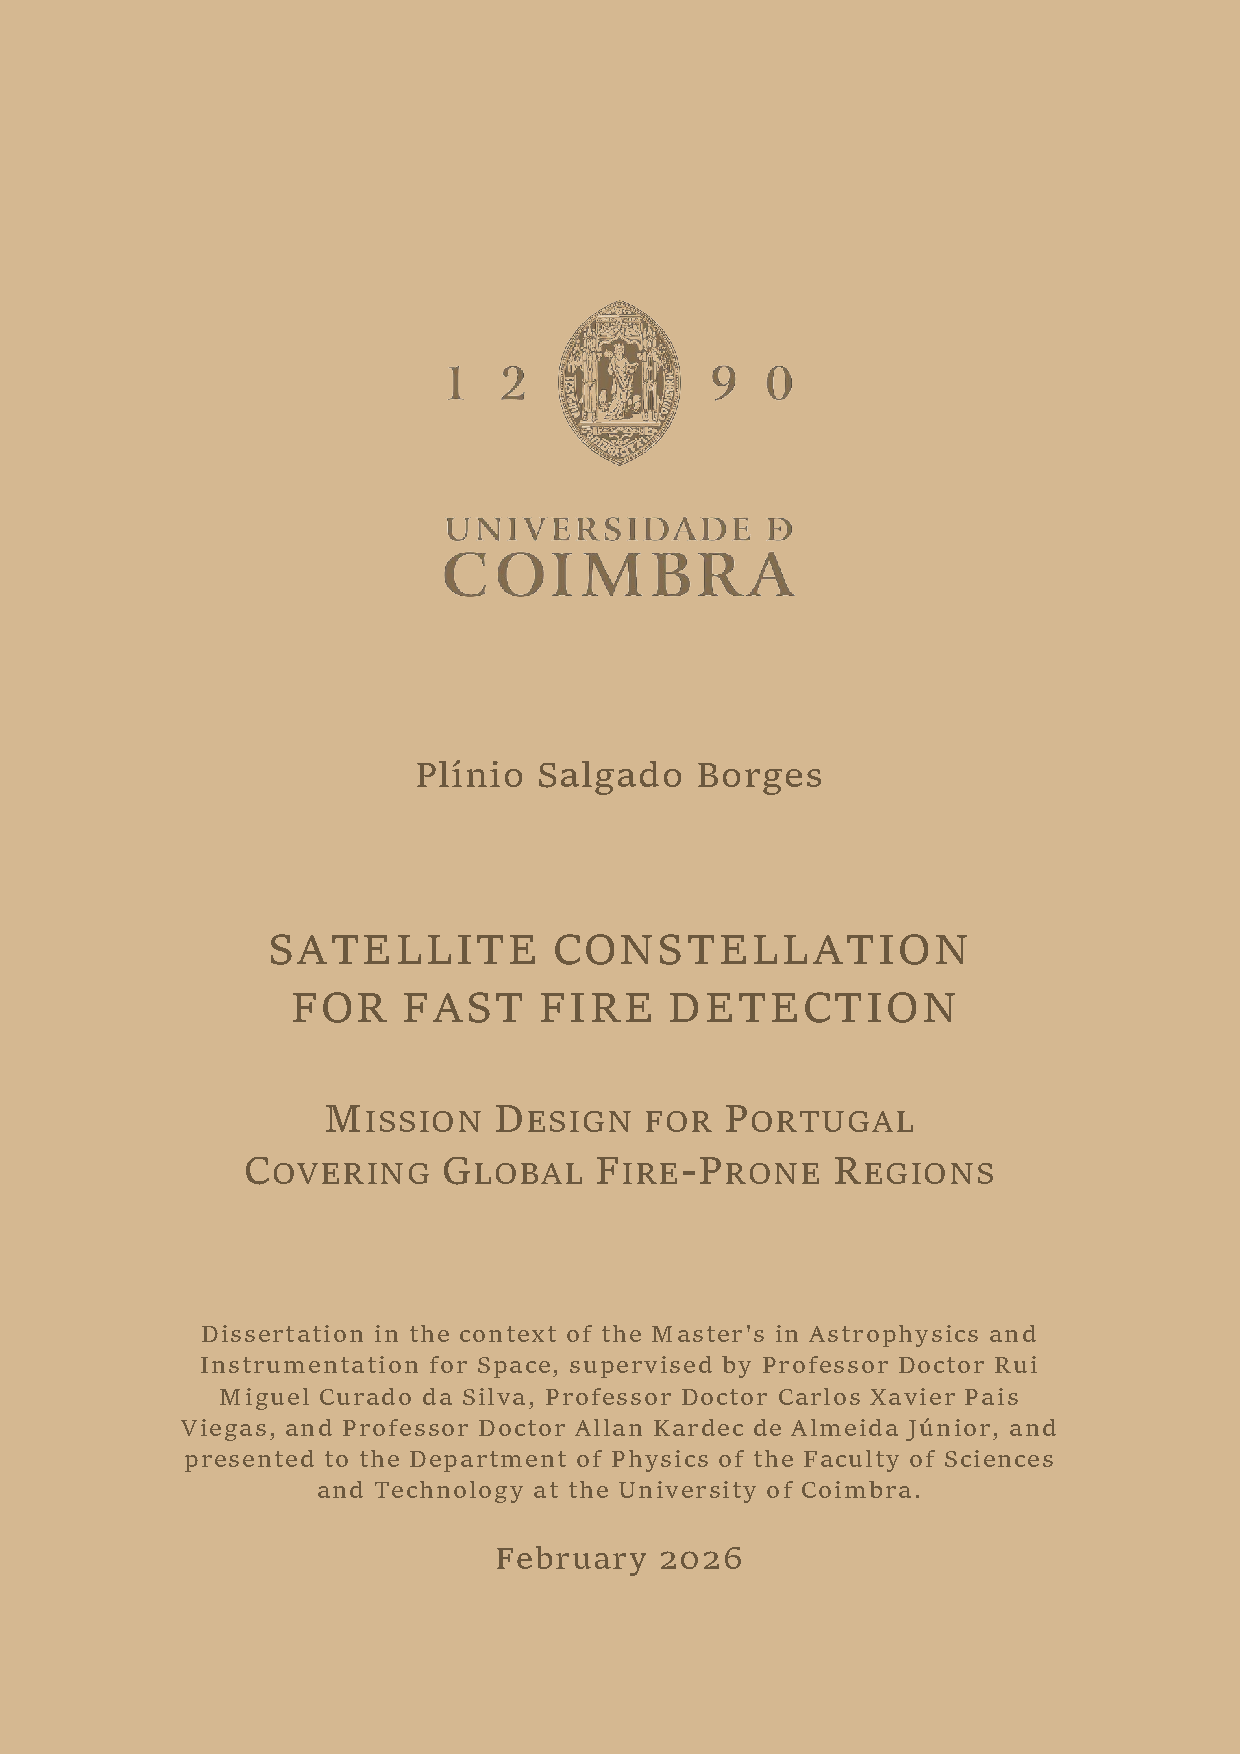
\includepdf[pages={-},pagecommand={}]{images/cover.pdf}
\newpage\thispagestyle{empty}

%\pagestyle{plain}

% --- TITLE PAGE ---
\begin{titlepage}
    \begin{center}
    % UC logo, no name
    
\includegraphics[width=0.34\textwidth]{images/UC_logos/UC_V_FundoClaro-negro.png}
    
    \vspace{0.2cm}
    {\huge{\myname\par}}
    
    % Thesis name
    \vspace{0.3cm}
    {\Huge{\textbf{\thesistitle}}\par}
    
    % Thesis subtitle
    \vspace{0.25cm}
    {\huge{\textsc{\thesissubtitle}}\par}

    \vspace{0.6cm}
    {\normalsize{\textbf{Supervisor:}\\{\supervisorname}\par}}
    
    \vspace{0.3cm}
    {\normalsize{\textbf{Co-Supervisors:}\\{\cosupervisorname}}}
    
    \vspace{0.4cm}
    {\footnotesize{\textbf{Jury:}\\[3pt]
    % TODO: Update jury member names here. This is a manual list.
    Prof.\ Dr. Jury Member 1\\
    Prof.\ Dr. Jury Member 2\\
    Prof.\ Dr. Jury Member 3\\
    Prof.\ Dr. Jury Member 4
    }}
    
    \vspace{0.5cm}
    {\footnotesize{Dissertation submitted in partial fulfillment for the\\degree of Master of Science in Astrophysics\\and Space Instrumentation.}}
    
    \vspace{0.2cm}
    {\small \statedate\par}    
    
    \end{center}
\end{titlepage}

% --- ACKNOWLEDGMENTS ---
\chapter*{Acknowledgments}
\addcontentsline{toc}{chapter}{Acknowledgements}
% ------------------------------------------------------------------
% Acknowledgements
% ------------------------------------------------------------------

% §1 — Institutional Support
% This work was partially funded by the Fundação para a Ciência e a Tecnologia (FCT), I.P., and developed at the Department of Physics of the University of Coimbra.

% §1b — Personal arc
This work grows out of a journey that began when, as a teenager in Brazil, I observed the planets through a telescope I had built with my own hands---deciding then to become a physicist. I started my studies at Brazil (UFMG) in 2010, spent time in Coimbra in 2011, and in Germany 2014, on this track specizlized in precision optics, working on systems ranging from Alzheimer's disease detectors to optical calibration of satellites (Sentinel-5). That path brought me back to Coimbra, more than a decade later, to complete the Master's in Astrophysics and Space Instrumentation (MAIE) that I had first glimpsed in 2011. Along that journey I witnessed the growing severity of wildfires in both Brazil and Portugal, and chose to dedicate this thesis to a problem that connects the two countries where I have built my life---and the planet I admire. To all who were part of this path---and who allowed me to move from someone who observes other planets to someone capable of conceiving missions to observe and protect the Earth---my most sincere gratitude.

% §2 — Supervisors
Among all, special recognition is owed to my supervisors, whose scientific guidance, intellectual rigour, and constant availability were decisive for the completion of this work.

To Professor Dr. Rui Miguel Curado da Silva, whose expertise in space systems made it possible to transform an initial idea---``Portugal faces wildfires; how can space instrumentation help?''---into a structured mission, connected to wildfire combat groups (ADAI) and to CubeSat fire-detection projects (FADO\footnote{F.A.D.O -- Fire Analysis \& Development Observatory, Concept Report CubeSat 2024, Team CSP-7-FADO.}), in which I participated and from whose colleagues I learned a great deal. His teaching in the space instrumentation course was essential for building the knowledge required to start this work, and his ability to connect people and institutions within the Portuguese space ecosystem was instrumental in defining the directions of this thesis and the future paths for fire-detection sensor development.

To Professor Dr. Carlos Xavier Paes Lidas, whose expertise in wildfire management and combat technologies---namely fire-spread modelling and the use of satellite imagery by firefighting authorities in Portugal---was fundamental in defining what the mission had to fulfil in the context of fire detection in Portugal. Part of the knowledge and data that informed this thesis was derived from two projects connected to Professor Carlos: the project IMFire---Intelligent Management of Wildfires\footnote{This work was carried out under the project IMFire---Intelligent Management of Wildfires, ref.\ PCIF/SSI/0151/2018, partially funded by national funds through the Ministry of Science, Technology and Higher Education, Portugal.}, and the project ForestSphere\footnote{This research was partially funded under the Protocol between Fundação para a Ciência e a Tecnologia and the Agency for Administrative Modernization, I.P.\ (AMA), through the project ForestSphere, ref.\ 2025.01496.DT4ST.}. It was also he who introduced me to Professor João Luís Ruivo Carvalho Paulo and the artificial-intelligence-based fire detection work within the FireSys project.

To Professor Dr. Alan Kardec de Almeida Júnior, whose knowledge of orbital mechanics was essential for advancing from basic mission requirements to high-fidelity models. He taught me to use GMAT, the mission-analysis tool developed at agencies such as NASA, and transmitted to me the fundamentals of celestial mechanics, perturbation forces, atmospheric drag, orbital stability, station-keeping, and the simulation tools required---foundations that constitute the simulation infrastructure presented here. I am equally grateful for his careful guidance in the writing and revision of this work.

To all three, my most sincere gratitude for the support, encouragement, and trust throughout this journey.

% §3 — Project Collaborators
I am equally grateful to Professor João Luís Ruivo Carvalho Paulo for the opportunity to work on the FireSys\footnote{This dissertation work was partially supported by the project FireSys -- ``Intelligent Decision Support System for Management of Wildfires'' with reference of operation 21378, operation code COMPETE2030-FEDER-02230700 on Balcão dos Fundos, funded by the Fundo Europeu de Desenvolvimento Regional (FEDER), through the Innovation and Digital Transition Program (COMPETE 2030) of Portugal 2030.} project on satellite-image-based fire detection using AI. From that project emerged the \emph{Watcher--Zoom} concept presented in this work.
I thank colleagues PhD\,(c) Dina Jahanianfard, who shared valuable insights on satellite image processing related to Sentinel-2 and the demonstration of the \emph{Watcher--Zoom} concept, and PhD\,(c) Matheus Fernandes Kovaleski, who collaborated on the code development.
I thank Dr.\ Timothée Vaillant for his suggestions regarding the defence presentation.
I also wish to thank the MAIE coordinators: Prof.\ Dr.\ Margarida Maria Lopes da Silva Camarinha, whose teaching in the Celestial Mechanics course provided the mathematical foundations and formalism present in this work, and Prof.\ Dr.\ Alexandre C. M. Correia for his support in navigating the decisions that helped define the thesis topic during the Master's and in bringing this work to completion.

% §4 — Scientific and Professional Formation
It is also important to acknowledge the experiences that built the foundations of this work before I arrived in Coimbra, starting in Brazil at UFMG. To Professor Dr. Ado Jório Vasconcelos, for the scientific training in optics at LabNS that constitutes my technical base and for believing in me at the start of my career, and to Professor Dr. Leandro Malard and colleagues at LabNS for their contributions to that formative in a unique environment. To Professor Renato Las Casas at the Observatório da Serra da Piedade, who taught me how to share the sky with others, and to Bernardo Riedel, who taught me the art of building telescopes. To Dr.\ Luiz Etrusco and colleagues at InventVision, for their support during my studies and in the development of advanced cameras. To Dr. Ivo Vieria and colleagues at LusoSpace, for showing me in practice how space systems are built.

% §5 — Colleagues and Friends
I wish to thank all the friends and colleagues who were with me at the University of Coimbra or who were part of this journey to the completion of the Master's, and who at the right moments helped me to relax, enjoy nature, and reflect on ideas.
To Flávia Amaral, astrophysicist and friend who can see vast distances in the universe that I can only begin to imagine, and who has accompanied this journey since 2010 at UFMG. To Pedro Pessoa, mathematician and friend whose mastery of geometry in many dimensions accompanied and enriched our studies in general relativity.
To my Master's friends though this journey ---Cláudia, Letícia, Snock, Aline, Guilherme, Carlos, João Werneck, Akel, Céci, Willian, Ronald, Rita, José Rodrigues, Fred, Maria João, Ricardo, Mariana Encarnação, Inês de Castro, Maria Campino, Fernanda, Joana, Cátia, Hortence, Diogo, Marcos, Angela, and Rubens Silva, Thiago Célio, Thiago Duarte, Filomeno, Eduardo Valadares, Ubirajará Agero, Paula, Renan, Alexandre, Emerson, Fabiano, Marcia, Hudson, Caciano, Lucas, Aroldo, Luiz, Wescley, Camila, Marina, Paola, Bruno, Erlan, André, Rafael, Luis, Kenji, André, Beto.
A special thank-you to Lara and Fig, for showing me that my technical skills in optical instrumentation, combined with space systems, could have a real impact on climate challenges---revealing a meaningful professional path, with consequences for the lives of many people and beings on this planet, and influencing the choice of the topic of this thesis.

% §6 — Family
Finally, I wish to express my deepest gratitude to my family.
To my father Joel and my mother Marisa, who supported me unconditionally at every stage---from the education they provided in Brazil to the decision to study abroad---and who, even at a distance, were never absent.
To my sisters Sabrina, Mariana, and Marina, for their constant encouragement and for always reminding me of what matters.
To all members of the family who contributed, throughout my life, with support, guidance, and the example that sustained effort is the surest way to accompanying our dreams.
This work is also yours.


% --- ABSTRACTS ---
\chapter*{Abstract}
\addcontentsline{toc}{chapter}{Abstract}
Lengthening fire-weather seasons and shifting vegetation flammability are driving unprecedented fire activity across Mediterranean Europe and other fire-prone regions. Portugal exemplifies this trend: extreme fire-weather indices have risen steadily since the late twentieth century, and projections indicate the most severe fire-weather class will cover much of the country by mid-century. Effective fire management demands rapid detection at scales fine enough to resolve individual fire fronts, yet no current or planned satellite system delivers both sub-hour revisit and metre-class resolution where it is needed most.

Geostationary sensors scan continental areas every 10--15~minutes but resolve only 2--3~km per pixel, while low-Earth-orbit missions achieve sub-30~m resolution at the cost of multi-day revisit intervals. This resolution--revisit--latency gap leaves fire-prone territories without timely, high-resolution space-based fire intelligence. The present work asks: \emph{What constellation design can close this gap, achieving roughly 30-minute revisit and approximately 6~m ground resolution over continental Portugal?} A secondary question is: \emph{What coverage does the constellation provide over global fire-prone regions?}

The study integrates fire-remote-sensing science, orbital mechanics, and high-fidelity numerical simulation.
A core study domain was first delineated by to Portugal's territory according it's fire season pattern, than a global study domain was defined to current fire-weather severity, establishing the geographical, spatial, and temporal requirements the constellation must satisfy.
An analytical survey of repeating ground-track orbits (RGTOs), generalised to arbitrary target latitudes, produced a family of RGTO modes for daily revisit in continental Portugal; from this group of orbital geometries the ratio $\tau = 15/1$ at approximately 488~km altitude and inclination ${\sim}\,40.2°$~was selected as best matched to the target latitude core study domain at center of Portugal, an resonating orbit around the city of Coimbra, providing the fastest revisit possible.
This selected orbitalmode was embedded in a Walker constellation framework. Parametric trades then explored the number of orbital planes, satellites per plane, and maximum sensor off-nadir viewing angle within a Walker-delta framework were allowed to optmized the revisit over the Portuguese core study domain.
The candidate constellations were propagated sing the high-fidelity General Mission Analysis Tool (GMAT) --- with a $8\times8$ geopotential, lunisolar perturbations, and atmospheric drag--- validating the orbital stability, observational-link pattern, temporal coverage, revisit statistics, and ground sampling distance over both the Portuguese core domain and a global fire-prone domain. 

The selected constellation---designated $C_{\text{Zoom}} = C_{15/5/72}$, comprising 15~satellites in 5~equally spaced orbital planes phased by $72^\circ$ of right ascending node, with 3 satellite per plane distributed $120^\circ$ of each by shifts in the true anomaly---achieves a mean revisit of approximately 21~minutes over Portugal with ground resolution below 6~m per pixel.
The repeating ground-track design delivers roughly $1.75\times$ the daily coverage time of a conventional sun-synchronous orbit at comparable altitude, effectively halving the fleet size that would otherwise be required.
A sensitivity analysis confirms that a $65°$ off-nadir sensor limit is essential: tightening it to cover only Portugal $30°$ keeping same cadence nearly doubles the required fleet to 27~satellites, underscoring wide-angle pointing as a key design driver for keeping the constellation compact.
Designed for Portugal, the coverage footprint extends naturally to all major fire-prone regions with exception of boreal region: the temperate belt---California, the broader Mediterranean basin, southern Africa, and south-eastern Australia---receives 6--7~hours of daily observation with worst-case revisit gaps of about 30 minutes, while tropical regions such as Amazonia, central Africa, and south-east Asia retain at least 3.5~hours per day with an average revisit around 40 to 50 minutes.
To expand the narrow field of view that metre-class resolution demands on a small platform, a \emph{Watcher--Zoom} tip-and-cue architecture is proposed: five existing geostationary fire-detection satellites provide coarse alerts every 10--15~minutes, cueing the nearest low-orbit spacecraft to steer its imager toward the hotspot and acquire high-resolution imagery.

No surveyed fire-detection constellation combines sub-30-minute revisit with metre-scale resolution over any examined fire-prone region. The architecture proposed here---fifteen satellites on a resonant orbit, guided by geostationary fire-watch assets---closes this gap for Portugal and extends meaningful coverage to every major fire-prone region on Earth, turning a national mission into a global cooperative-observation platform.


The study integrates fire-remote-sensing science, orbital mechanics, and high-fidelity numerical simulation. A core study domain was delineated over Portugal according to its fire-season pattern; a global domain was then defined by current fire-weather severity, establishing the geographical, spatial, and temporal requirements. An analytical survey of repeating ground-track orbits (RGTOs), generalised to arbitrary target latitudes, produced a family of modes for daily revisit over Portugal; from this set the ratio $\tau = 15/1$ at approximately 488~km altitude and ${\sim}\,40.2°$ inclination was selected as best matched to the core domain centred on Coimbra, providing the fastest revisit. This orbital mode was embedded in a Walker-delta framework; parametric trades explored the number of planes, satellites per plane, and maximum off-nadir angle to optimise revisit. Candidate constellations were propagated with the General Mission Analysis Tool (GMAT)---$8\times8$ geopotential, lunisolar perturbations, and atmospheric drag---validating orbital stability, coverage, revisit statistics, and ground sampling distance over both domains.

The selected constellation---$C_{\text{Zoom}} = C_{15/5/72}$, 15~satellites in 5~planes phased by $72^\circ$, 3~per plane at $120^\circ$ true-anomaly spacing---achieves a mean revisit of approximately 21~minutes over Portugal with ground resolution below 6~m. The repeating ground-track delivers roughly $1.75\times$ the daily coverage of a sun-synchronous orbit at comparable altitude, effectively halving the required fleet. A sensitivity analysis confirms that the $65°$ off-nadir limit is essential: tightening it to $30°$ nearly doubles the fleet to 27~satellites, underscoring wide-angle pointing as a key design driver. The coverage extends naturally to all major fire-prone regions except the boreal belt: temperate zones---California, the broader Mediterranean, southern Africa, south-eastern Australia---receive 6--7~hours of daily observation with worst-case gaps of about 30~minutes, while tropical regions retain at least 3.5~hours per day with average revisit of 40--50~minutes. To compensate the narrow field of view that metre-class resolution demands, a \emph{Watcher--Zoom} tip-and-cue architecture is proposed: five geostationary fire-detection satellites provide alerts every 10--15~minutes, cueing the nearest low-orbit spacecraft to image the hotspot at high resolution.

% \vspace{1em}
% \noindent\textbf{Keywords:} satellite constellation, fire detection, repeating ground-track orbit, mission design, fire detection, Portugal, Earth observation

% --- INSPIRATIONAL QUOTE ---
\chapter*{}
\setlength\epigraphwidth{14.5cm}
\setlength\epigraphrule{0pt}
\makeatletter
\patchcmd{\epigraph}{\@epitext{#1}}{\itshape\@epitext{#1}}{} {}
\makeatother
\vspace*{\fill}
\epigraph{%
\footnotesize\upshape%
February 14, 1990.\\[\medskipamount]
Beyond the orbit of Neptune,\\
after a last encounter with Saturn,\\
Voyager~1 turned its camera homeward\\
and captured the whole of Earth\\
as a single dot, a speck of light.%
\par\medskip \medskip
``From this distant vantage point, the Earth might not seem of any particular interest. But for us, it's different. Consider again that dot. That's here. That's home. That's us. On it everyone you love, everyone you know, everyone you ever heard of, every human being who ever was, lived out their lives.
[\ldots] Our planet is a lonely speck in the great enveloping cosmic dark. In our obscurity, in all this vastness, there is no hint that help will come from elsewhere to save us from ourselves. The Earth is the only world known so far to harbor life. There is nowhere else, at least in the near future, to which our species could migrate.
[\ldots] To me, it underscores our responsibility to deal more kindly with one another, and to preserve and cherish the pale blue dot, the only home we've ever known.''}{Carl Sagan, \textit{Pale Blue Dot} (1994)}
\vspace*{\fill}

%% --- TABLE OF CONTENTS AND LISTS ---
\pagestyle{plain}
\tableofcontents

% \chapter*{List of Acronyms}
%\addcontentsline{toc}{chapter}{List of Acronyms}
% % TODO: Define your acronyms here.
% Use the format: \acro{ACRONYM}{Full Name}
% Then, use \ac{ACRONYM} in your text.
% The first use will expand the acronym, and subsequent uses will show the acronym only.
\begin{acronym}[UC]
    \acro{UC}{University of Coimbra}
    \acro{MSc}{Master of Science}
\end{acronym}

% Example usage to ensure acronym is defined
% \ac{DEA}

\listoffigures
\listoftables

% ── List of FIXMEs (remove before final submission) ──
\listoffixmes
%% ======================================================================
%% MAINMATTER
%% ⚑ Purpose: main thesis content (Arabic page numbers, numbered chapters)
%% ======================================================================
\mainmatter

% --- ADD NEW CHAPTERS BELOW ---
% \chapter{[Your Chapter Title]}
% \label{chap:[your-label]}
% \input{chapters/[your-file]}


% --- Part1: INTRODUCTION & BACKGROUND ---
% ----------------------------------------

\part{INTRODUCTION \& BACKGROUND}
\label{chap:partI_intro_back}

% --- CHAPTER 1: INTRODUCTION ---
\chapter{\texorpdfstring{\emph{Introduction}}{Introduction}}\label{c1_introduction}

As planetary boundaries are progressively transgressed ---in particular the climate and biosphere-integrity frontiers--- Space Earth Observation Sensors are evolving to match the pace of environmental change and are becoming essential for both mitigation and adaptation.
This thesis contributes to that emerging capability through the mission design of a small-satellite constellation for fire detection, targeting sub-30-minutes revisit and metre-scale ground resolution over continental Portugal with coverage extending to global fire-prone regions, and positions the system within the \emph{Planetary Boundaries} framework (Fig.~\ref{fig:intro_planetary_boundaries}) as a sensor providing a fire-information link, $\mathcal{L}_{\text{fire}}$, connecting the spacecrafts to two ground domains ---fire-stressed ecosystems and human wildfire combat response--- shortening the feedback loop from environmental change to operational action \cite{rockstrom2009safe, richardson2023earth,sakschewski_planetary_2025,lenton_gaia_2018}.


\begin{figure}[H]
    \centering
    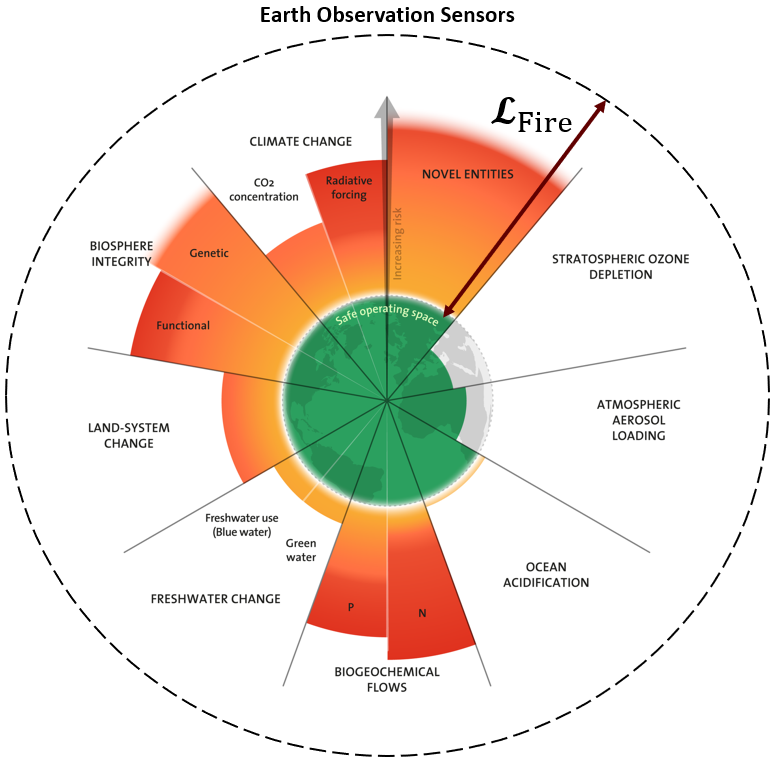
\includegraphics[width=0.65\linewidth]{images/planetary_bondaries_2025_9frontires_7_crossed_Lfire.png}
    \caption{\footnotesize{Planetary boundaries showing the safe operational limit of the Earth system, with the climate boundary transgressed and the biosphere integrity boundary under high risk. \cite{sakschewski_planetary_2025}}}
    \label{fig:intro_planetary_boundaries}
\end{figure}


% \begin{figure}
%     \centering
%     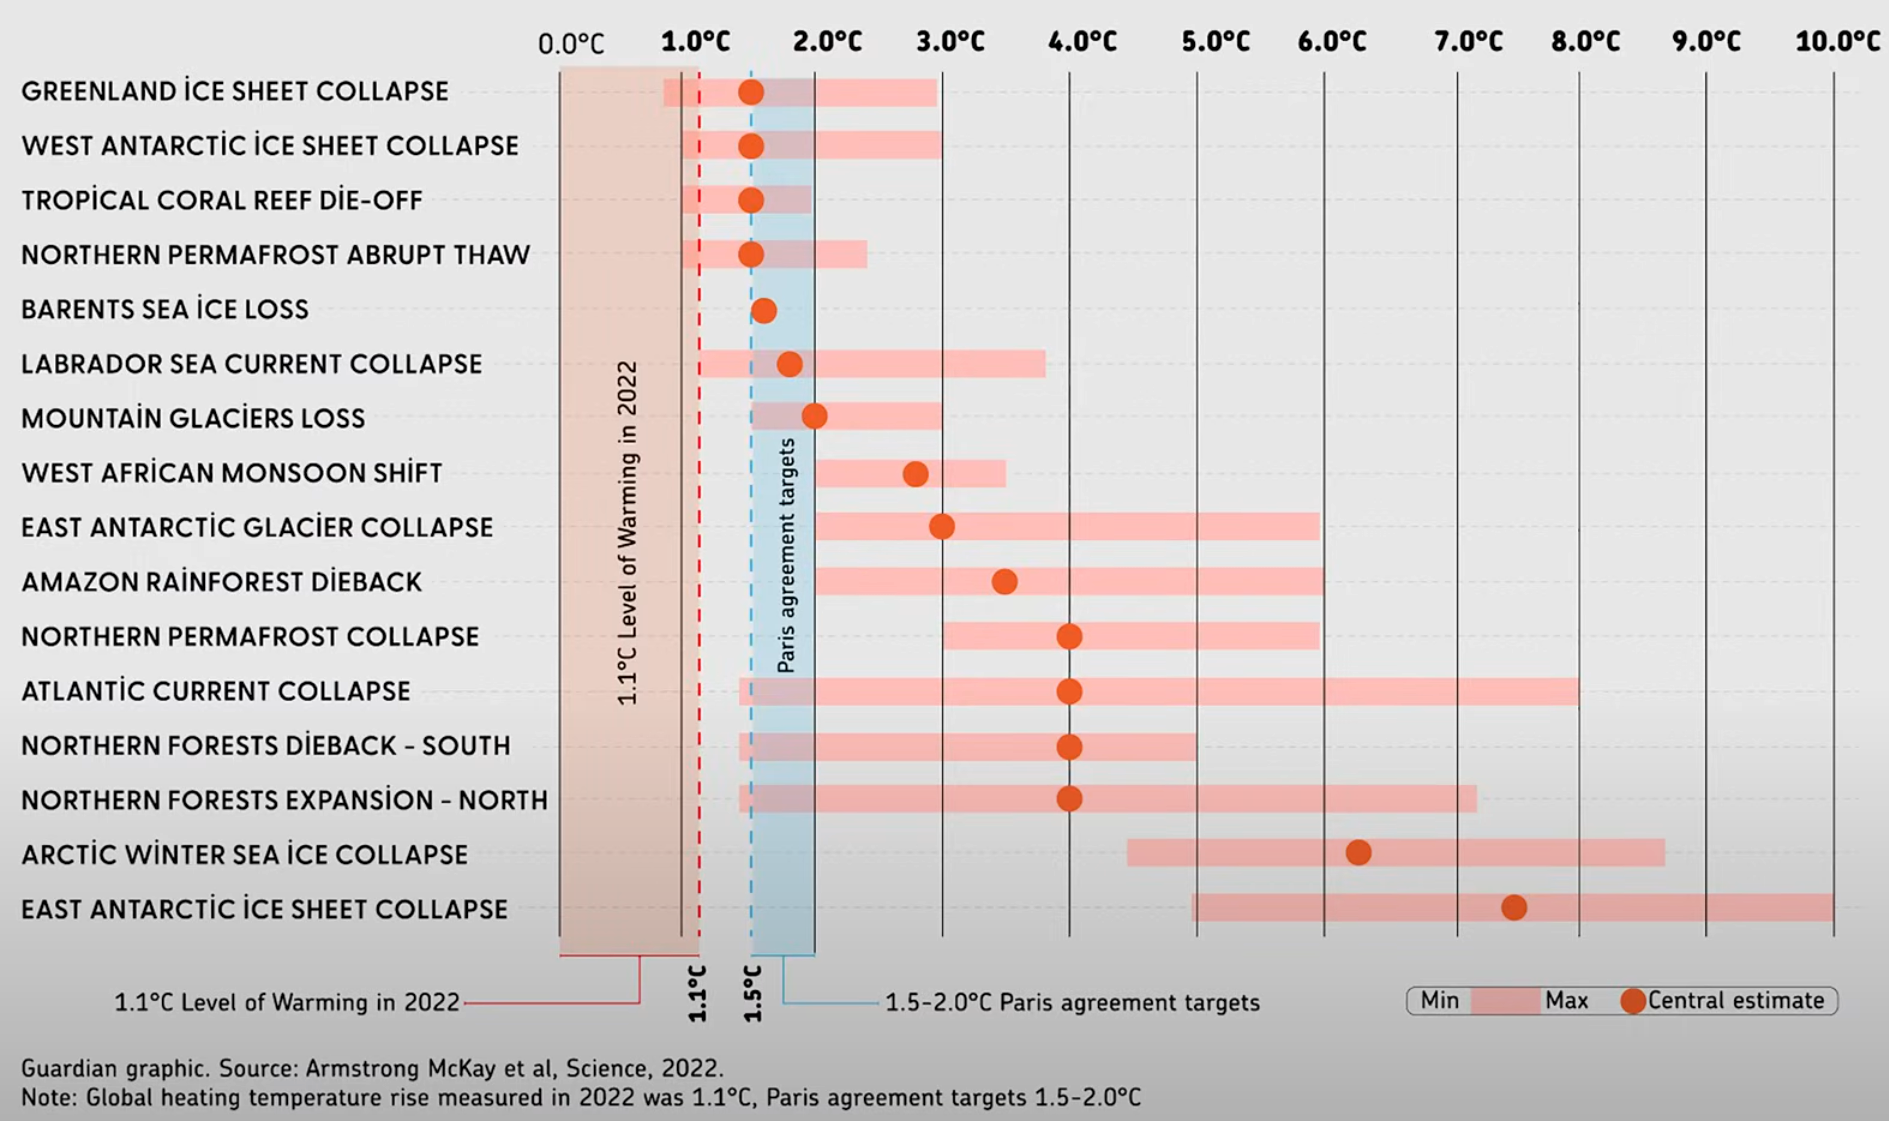
\includegraphics[width=1\linewidth]{images/tiping_points_info.png}
%     \caption{Enter Caption}
%     \label{fig:intro_tipping_points}
% \end{figure}

This thesis mission is also situated within the scope of \emph{Intergovernmental Panel on Climate Change (IPCC) AR6}, as a \emph{cross-sectoral transition system} (items C.2.11, C.2.12, and C.2.13)---an \emph{adaptive response} toward \emph{sustainable and resilient states} in \emph{urban infrastructures}, \emph{terrestrial and coastal 	ecosystems}, and in \emph{social choices/transitions}, providing  \emph{Disaster Risk Management} and \emph{Early Warning Systems}. 
\cite{ipcc2018sr15,ipcc2022wg2,ipcc2023syr}.


\emph{Why acting now is urgent?} In light of the \emph{Paris
	Agreement (Art. 2, UNFCCC)} and \emph{IPCC SR1.5}, limiting warming to
\emph{1.5 °C} requires \emph{net-zero CO\textsubscript{2} around 2050} \cite{ipcc2018sr15,unfccc2015paris}.
The \emph{Glasgow Climate Pact (COP26)} and the
\emph{UNFCCC Global Stocktake} indicate that current progress is
\emph{off-track} \cite{unfccc2021glasgow,unfccc2023gst}, while the \emph{World
	Meteorological Organization (WMO)} reports annual global means near the
\emph{1.5 °C} level in \emph{2023--2024} (temporary exceedances)
\cite{wmo2024state,wmo2025press}. Within \emph{Planetary Boundaries}, the
\emph{climate boundary} is \emph{transgressed}, raising the risk of
cascading impacts; warming around \emph{1.5 °C} increases the
likelihood of \emph{losses of resilience} and \emph{abrupt changes}
\cite{richardson2023earth,lenton2019tipping,armstrong2022tipping}.

% \begin{figure}[H]
%     \centering
%     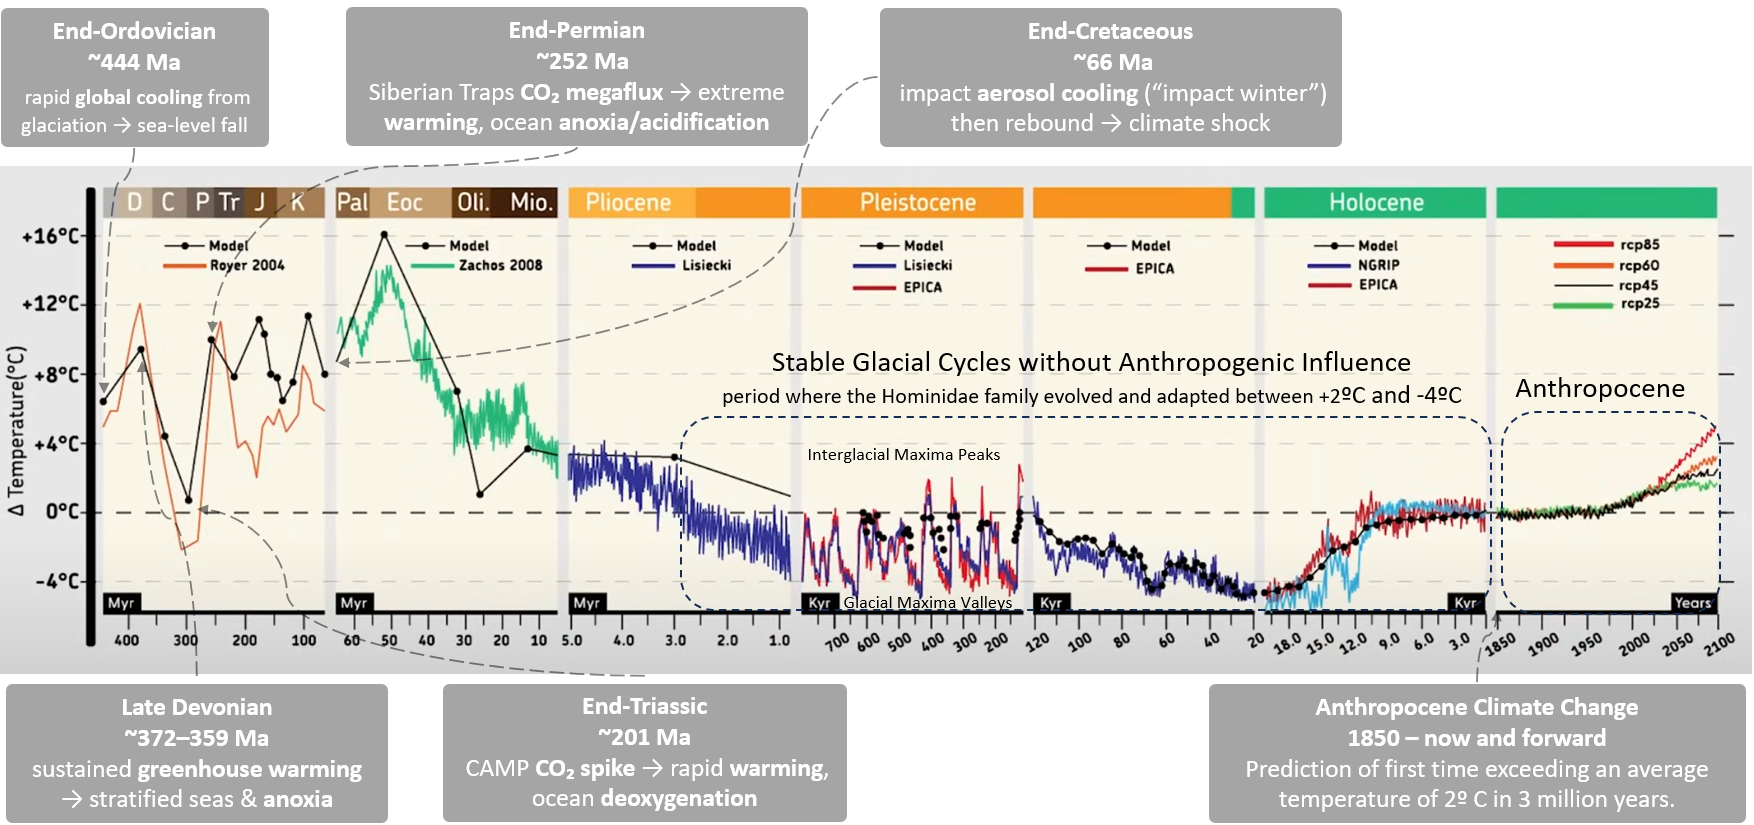
\includegraphics[width=1\linewidth]{images/paleclima_Dt_mass_extitions.png}
%     \caption{\footnotesize{Paleo-weather temperature variation, mass extinctions, and the Anthropocene fire signal.
% Global mean temperature anomalies from multiple compilations show large coincident with the \textbf{Big Five mass extinction}s:  \textbf{I)End-Ordovician (~444 Ma)} : abrupt cooling and glaciation; \textbf{II)Late Devonian (~372–359 Ma)}: greenhouse warming pulses superimposed on a long cooling trend, driving ocean stratification/anoxia; \textbf{III)End-Permian (~252 Ma)}: CO$_2$ megaflux and extreme warming leading to widespread anoxia/acidification; \textbf{IV)End-Triassic (~201 Ma)} rapid volcanogenic warming with ocean deoxygenation; \textbf{V)End-Cretaceous (~66 Ma)}: impact winter (short cooling) followed by rebound warming. The Pleistocene section exhibits \textit{quasi-periodic glacial–interglacial cycles} (early 41 kyr, late ~100 kyr “sawtooth”) within which hominins evolved. During the Holocene, a period with stable temperatures that coincides with and facilitates the development of agriculture and the flourishing of larger human societies. During this epoch, we find the \textbf{Anthropocene, which has as one of its marks an unprecedented, human-driven warming rate}, with high-emission pathways possibly exceeding +2 °C, warmer than any time in ~3 Myr and aligned with multiple planetary-boundary transgressions. In this work, we interpret the documented increase in active fire as an early stress signal of declining biosphere integrity. We consider the Anthropocene impact on fire activity, fire weather index, and burned-area dynamics as one of the markers of a trajectory consistent with the onset of a potential future Sixth Mass Extinction without rapid mitigation.}}
%     \label{fig:paleoclima_mass_extinctions}
% \end{figure}

% \begin{figure}[H]
%     \centering
%     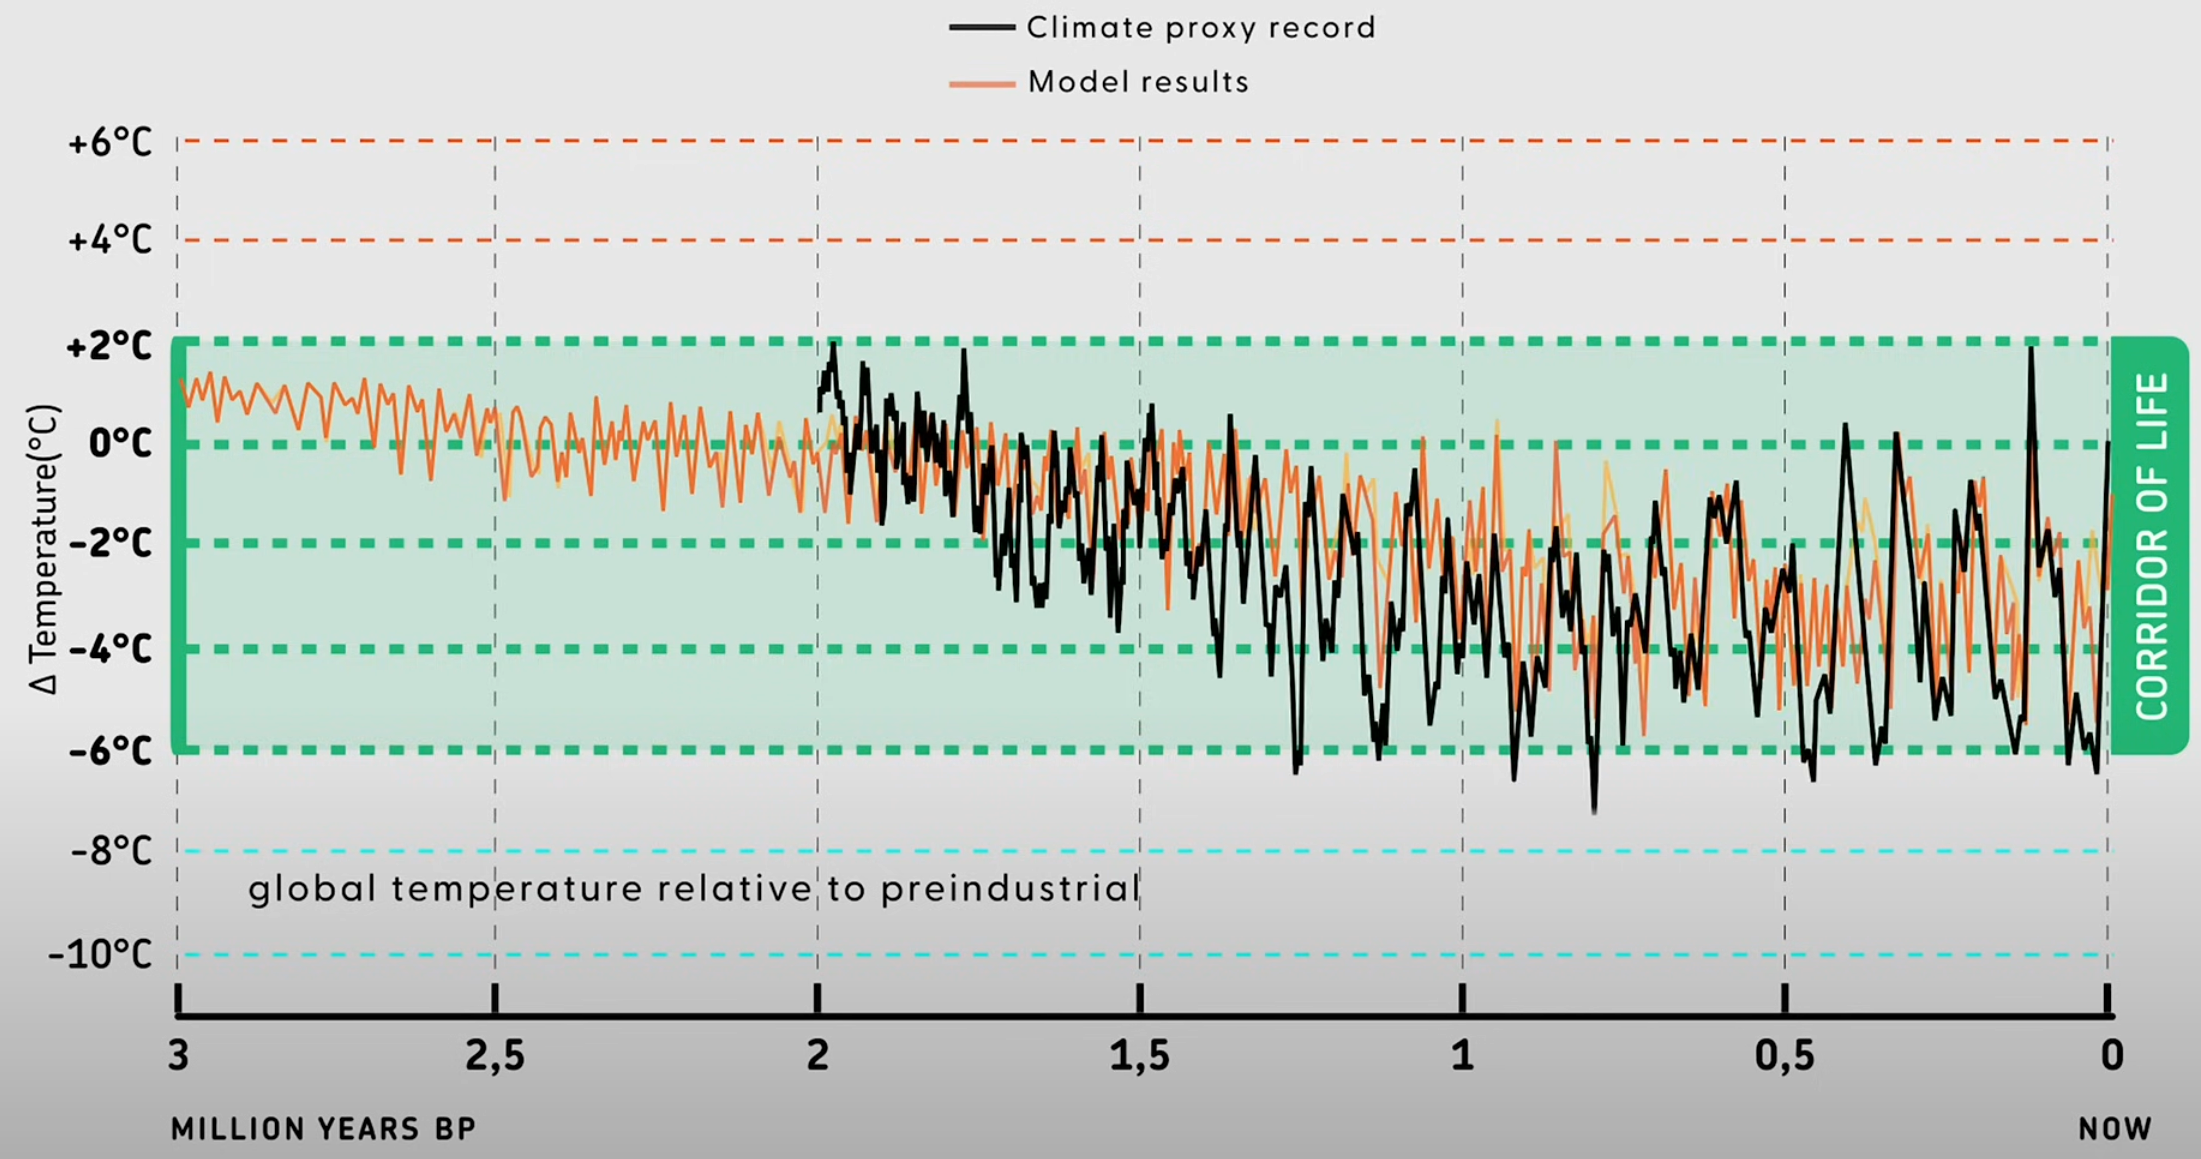
\includegraphics[width=1\linewidth]{images/life_corridor.png}
%     \caption{Enter Caption}
%     \label{fig:intro_life_corridor}
% \end{figure}

%\begin{figure}[H]
%    \centering
%    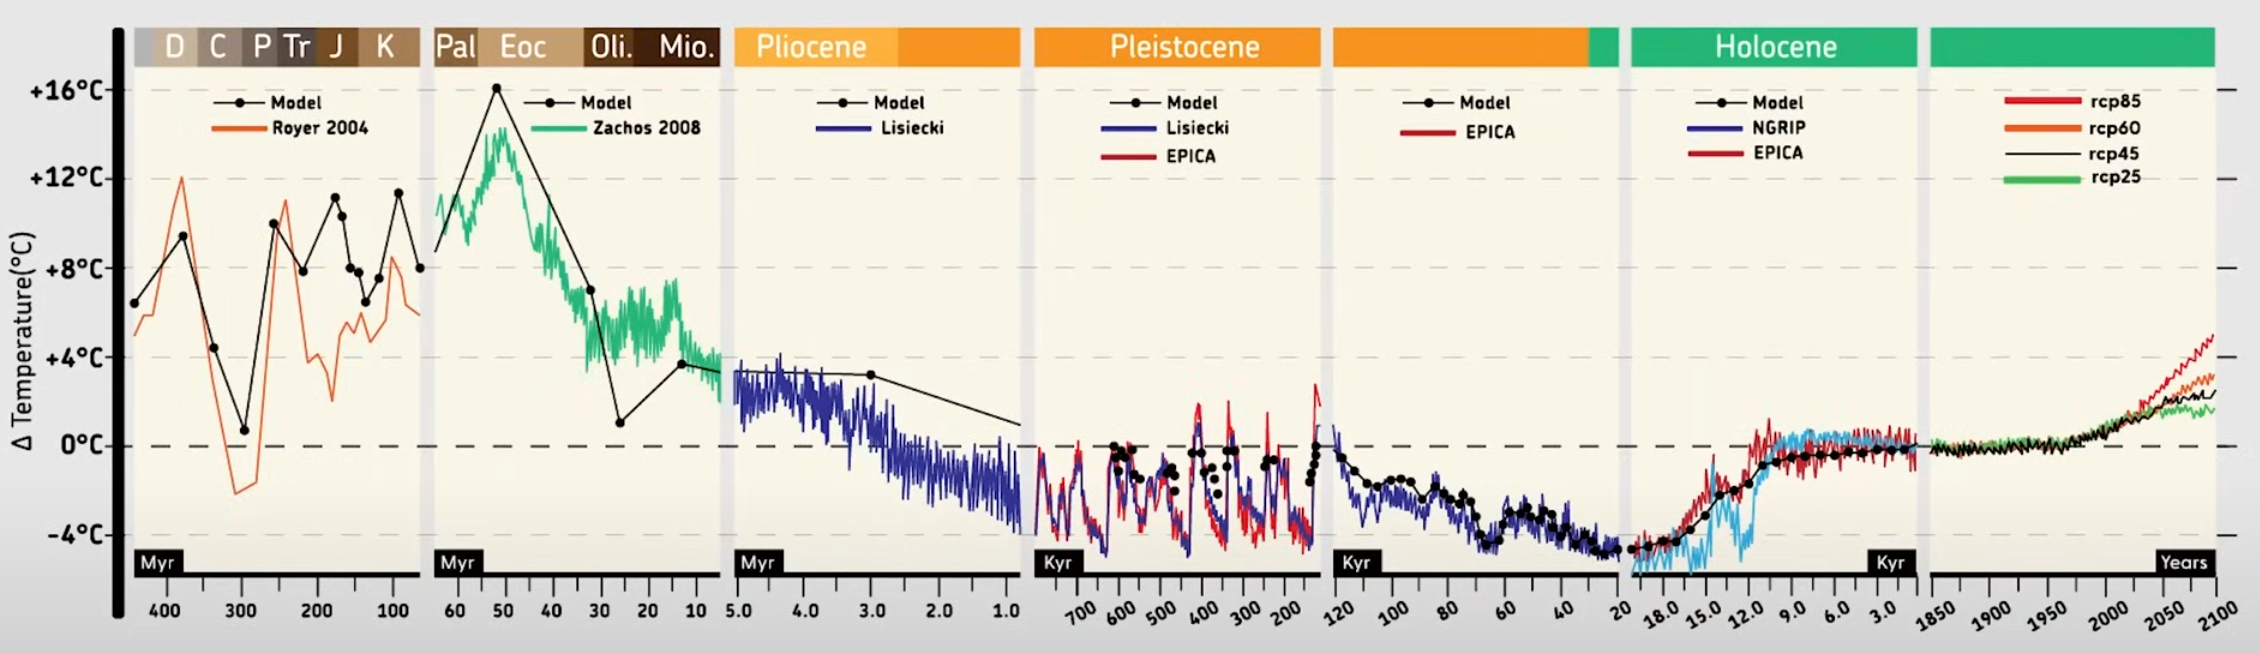
\includegraphics[width=1\linewidth]{images/paleoclimateDT.png}
%    \caption{Enter Caption}
%    \label{fig:placeholder}
%\end{figure}

%\begin{figure}
%    \centering
%    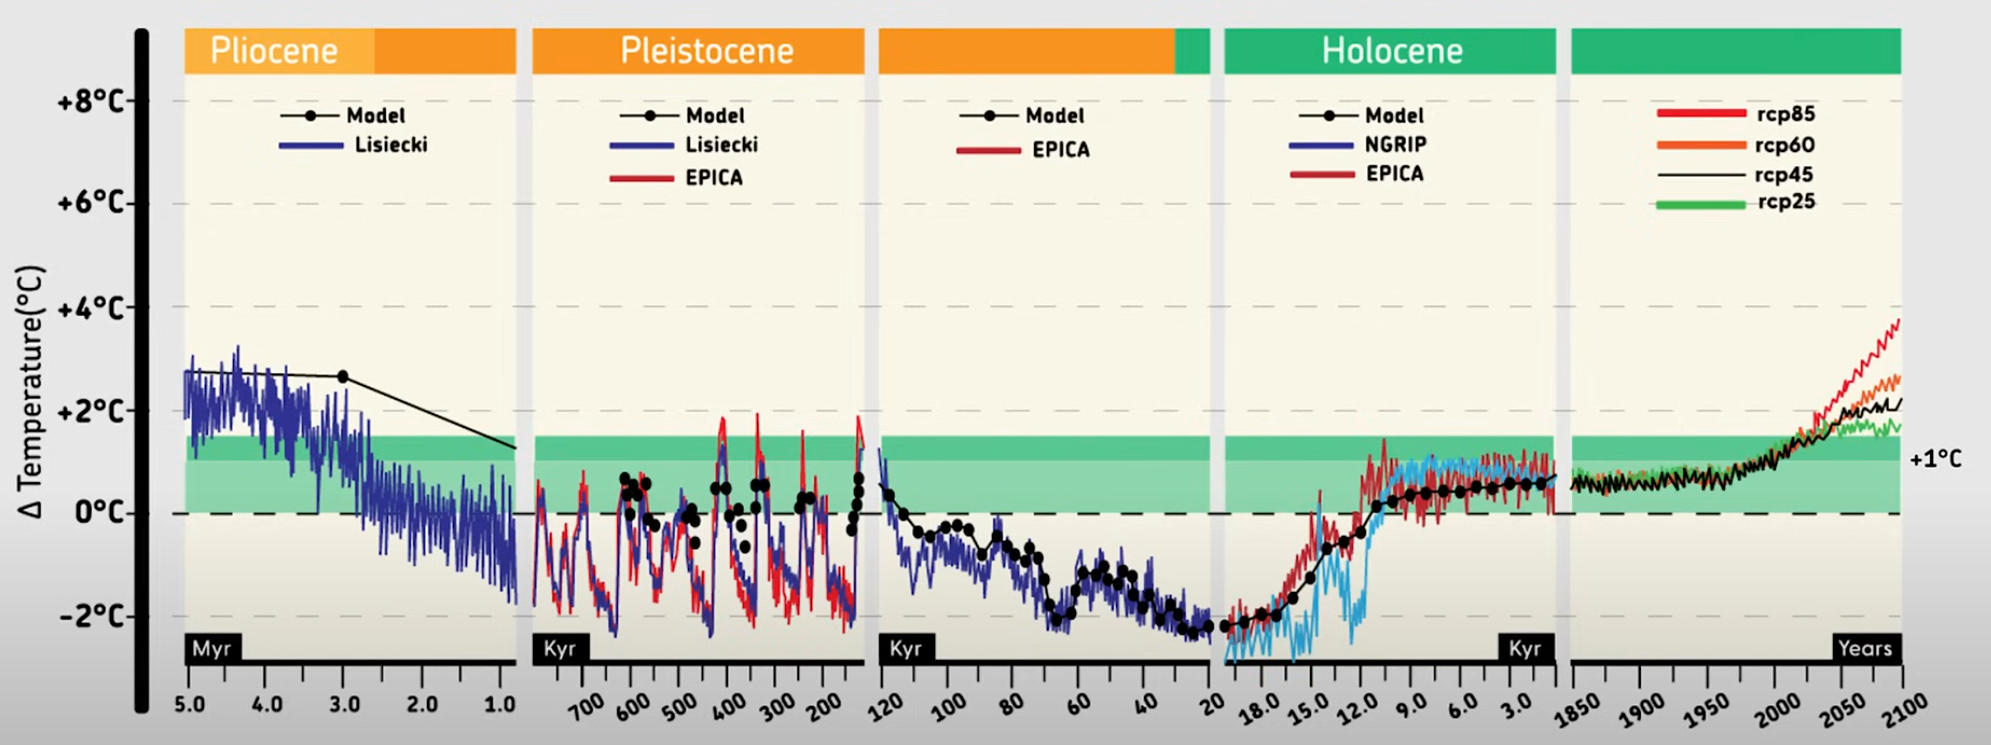
\includegraphics[width=1\linewidth]{images/paleoclimateDT_life_corridor.png}
%    \caption{Enter Caption}
%    \label{fig:placeholder}
%\end{figure}

% \begin{figure}
%     \centering
%     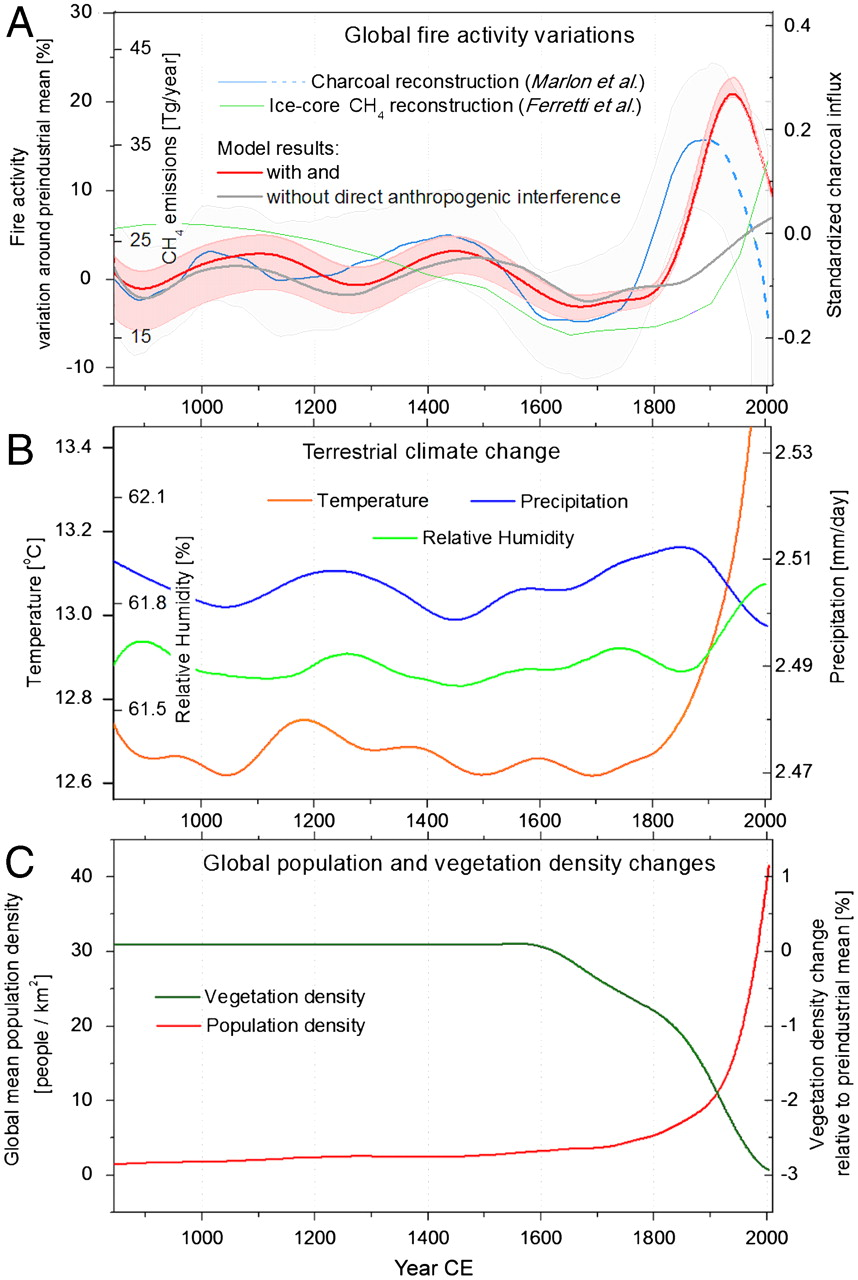
\includegraphics[width=0.7\linewidth]{images/paleo_globa_fire_activityVSpopulation_temperature.png}
%     \caption{Global fire activity, climate, vegetation, and population. (A) Modeled global fire activity variations (SI Text) with (red line) and without (gray line) direct anthropogenic influence (ignition and suppression): Red-shaded area represents uncertainty in the anthropogenic effect assumptions (SI Text); ice-core methane fire emissions reconstruction (green line) (17) and charcoal-based global fires reconstruction (blue line) with gray-shaded confidence interval (12) and blue dashed line indicating increased uncertainty in the late 20th century reconstructions. (B) GISS GCM annual means of the terrestrial area surface temperature (orange line), precipitation (blue line), and relative humidity (green line). (C) Global mean population (red line) and vegetation (green line) densities (11).}
%     \label{fig:intro_fire_activity_population}
% \end{figure}
In Earth System science, the \emph{Anthropocene} is an era where human activities act as a planetary force influencing geological, climate, and biospherical systems. This period is marked by extreme or
frequent fires that signal \emph{systemic stress} and possible \emph{critical transitions} in ecosystems and societies
\cite{bowman2020fires,scheffer2009early}. Therefore, socio-ecological
systems must adapt rapidly to conditions that favour intense fire seasons; we
need forecasts and alerts with \emph{high spatial--temporal detail},
operating \emph{day/night} (visible/thermal infrared) and in \emph{any weather}
(microwave/SAR), across urban and rural regions. To this end, it is necessary
to \emph{develop a satellite constellation for fire-meteorology monitoring
with high spatial and temporal resolution}, which---when coupled with other
models and forecasting systems---can provide:
\begin{enumerate}\setlength{\itemsep}{0pt}\setlength{\parskip}{0pt}\setlength{\parsep}{0pt}
\item \textbf{Diagnosis of fire-resilience states \inlineReq{R1}}\footnote{[\rightarrow R\#] refers to the requirement number \# being created at this point. Full description of the requirment is found in the end of each chapter, i.e \S \ref{sec:requirements_level1}.The requirements framework adopted in this work is detailed in Appendix~\ref{app:se_approach} and \S\ref{sec:requirements_level1}.}
\item \textbf{Anticipation of ignitions \inlineReq{R2}}
\item \textbf{Near--real-time identification of hotspots \inlineReq{R3}}
\item \textbf{Near--real-time monitoring of fire-front evolution \inlineReq{R4}}
\item \textbf{All weather, cloud/smoke-penetrating, day/night capability \inlineReq{R5}}
\end{enumerate}


Thus, the constellation gives responders the ability to \emph{suppress
	hotspots as early as possible} and to focus resources where most needed,
given predicted fire evolution and risk---reducing losses of
\emph{biodiversity} and \emph{CO\textsubscript{2} sinks}, which are crucial for
limiting warming and moderating future fire seasons \cite{kelly2020fire}.

As a first step, we propose a \emph{regional-coverage satellite
	constellation design demonstration} for the \emph{Iberian Peninsula
	(continental Portugal)}\inlineReq{R6}. This is a Mediterranean hotspot where wildfire danger
and impacts are among Europe's highest, reflecting strong couplings
between urban systems and fire-prone ecosystems that affect
environmental quality and public well-being \cite{sanmiguel2018fires,costa2020wildfire,turco2019drivers}. From
this \emph{seed constellation}, expansion to other regions is
envisaged.

\section{Motivation \& Problem Statement}\label{sec:motivation}

The motivation for this work can be understood in five points which will be detailed in the following sub-chapters and concluded with the problem statement of this work, they are: first, the climate crisis, which is increasing fire danger; second, the fact that Portugal is a region where fire lines are zoned; third, a need of strengthen of the capabilities wildfire combat in Portugal; fourth, the Portuguese services uses satellite imagery with long revisit period for fire prediction, this high latency image input  directs to the final motivation point,  leading to low fidelity fire spread models predictions and a higher risk of ineffective firefighting. The low fidelity is due the fact the weather is dynamic and the changes between measurments are not certain, the uncertain grows with time, increasing the impression of the models, therefor high cadence satellite imaginary is needed to avoid low fidelity.  These are the key points that motivate the development of a high-temporal and spatial satellite constellation to improve fire prediction and management in Portugal. 

\subsection{Climate crisis with increased fire danger} 

Anthropogenic warming has lengthened fire-weather seasons globally from ${\sim}60$\,days\,yr$^{-1}$ (2025 baseline) toward ${\sim}70$\,days by mid-century and ${\sim}78$\,days by 2100, while the frequency of extreme fire-weather days ($\mathrm{FWI}_{95\mathrm{d}}$) has risen in step \cite{jones_global_2022,abatzoglou_global_2019}. The signal is strongest in the Mediterranean, where fire-season length is projected to grow from ${\sim}90$ to ${\sim}150$\,days\,yr$^{-1}$ and extreme days from ${\sim}30$ to ${\sim}75$\,days\,yr$^{-1}$ over the same horizon. Although \emph{global} burned area has declined since 2001---driven primarily by African savanna land-use change---regional burned area in Mediterranean and boreal forest biomes has increased, with Mediterranean projections of $+40$--$187\%$ under $1.5$--$3\,^{\circ}$C warming scenarios \cite{jones_global_2022,andela_humandriven_2017,turco_exacerbated_2018}.

Senande-Rivera et al.\ classified fire-prone regions worldwide into four K\"oppen--Geiger-based fire-climate classes, each stratified by recurrence: \emph{recurrent} ($>7$ fire-prone years per decade), \emph{occasional} ($3$--$7$), and \emph{infrequent} ($<3$) \cite{senande-rivera_spatial_2022}. Their projections (2070--2099) shown that some presently infrequent zones shift to occasional and occasional zones tend to become recurrent, enlarging the global fire-prone area (Fig.~\ref{fig:fire_prone_global_now_future}). This classification is adopted in Section~\ref{sec:generalized_study_domain} to define the constellation's global study domain $\mathcal{D}_{\text{Global}}$ fire-prone target mask.

\begin{figure}[H]
    \centering
    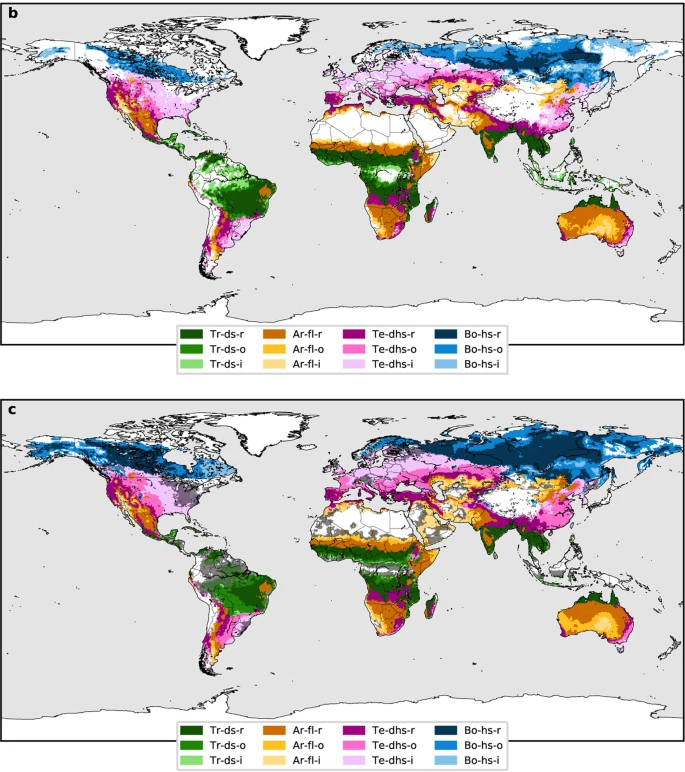
\includegraphics[width=0.9\linewidth]{images/fire_prone_global_now_future.png}
    \caption{\footnotesize{Present and projected global fire-prone climatic regions. (b)~Present fire-climate regions (1996--2016). (c)~Projected fire-climate regions (2070--2099) under CMIP5 GCMs; shaded grey indicates $<$75\% model agreement. Four fire-climate classes---Tropical-Dry Season (Tr-ds), Arid-Fuel Limited (Ar-fl), Temperate-Dry Hot Season (Te-dhs), Boreal-Hot Season (Bo-hs)---are each subdivided by fire-prone year recurrence per decade: recurrent~(r,\,$>$7), occasional~(o,\,3--7), infrequent~(i,\,$<$3). Adapted from Senande-Rivera et al.\ \cite{senande-rivera_spatial_2022}.}}
    \label{fig:fire_prone_global_now_future}
\end{figure}


% \subsection{Recent increase of fire danger (global/European signal).}

% Assessments show robust increases in \emph{fire weather}, longer
% seasons, and projected growth in burned area under continued
% warming---signals that are particularly strong across Iberia and the
% broader Mediterranean \cite{ipcc2023syr,jolly2015climate}.

\subsection{Portugal: recurrent, severe wildfires.} 


Continental Portugal exemplifies these challenges, with repeated extreme seasons;
\emph{2017} stands out as catastrophic in scale and impacts (area
burned, 116 fatalities and hundreds wounded), motivating improved observation and response
capability \cite{sanmiguel2018fires,turco2019drivers,cti2017pedrogao}. A prominent example with 66 fatalities is the
\textbf{17 June 2017 Pedrógão Grande} event: under \emph{extreme	pyrometeorology}, the convective column collapsed, producing a \emph{downburst} that drove the fire front at \emph{\textasciitilde15 km h$^{-1}$ for \textasciitilde10min}---overwhelming decision windows, for reference, human average running speed is \textasciitilde10 km h$^{-1}$---at a time when \emph{near--real-time orbital nowcasting} was not integrated into operations \cite{cti2017pedrogao}.

In 2025, Portugal’s burned area approached \(\sim\)280{,}000~ha (\(\approx\)3\% of national territory), rivaling 2017, with major fires affecting Castelo Branco (incl. the Fundão area) \cite{portugal_area_2025, effisPRTstats, reuters2025eu,}. Evidence from the Mediterranean shows that land abandonment and the resulting increases in fuel load/connectivity elevate fire hazard and the likelihood of large events; abandoned farmland transitioning to shrubland is particularly at risk \cite{schworer2024medfire,kirkland2024med}. Species composition also modulates hazard: eucalypts display high flammability traits that can promote intense fire behaviour, though in Portugal the expansion of eucalypt plantations alone does not explain interannual burned area once weather and other drivers are accounted for \cite{younes2024eucflamm,fernandes2019eucalypt}. These dynamics strengthen the case for high-cadence Earth observation to support early detection, nowcasting, and operational decision-making during transitions toward more resilient urban–rural–forest socio-ecosystems.

\begin{figure}[H]
    \centering
    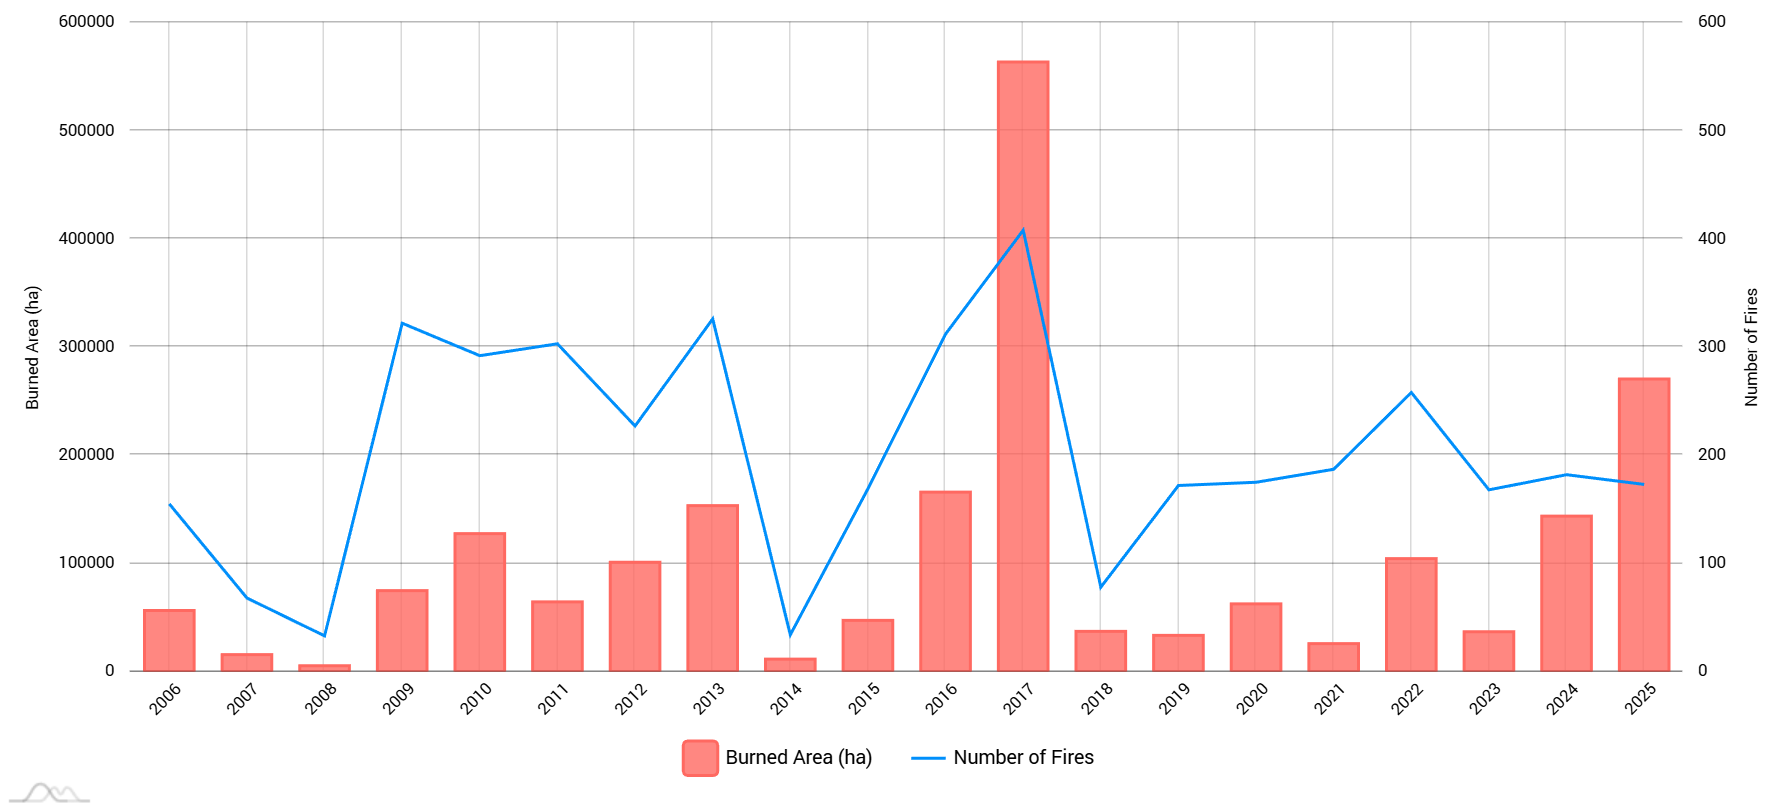
\includegraphics[width=1\linewidth]{images/burned_area_estimates-by-country_PRT_2006_2024.png}
    \caption{\footnotesize{EFFIS annual burned area statistic temporal series for Portugal. Two charts of temporal series between 2006 and Setember-2025 showing burned area and number of Fires.\protect\footnotemark}}
    \label{fig:burned_area_estimative_pt}
\end{figure}
\footnotetext{Reproduced from Abatzoglou, J.~T., Williams, A.~P., \& Barbero, R. (2019), \textit{Geophys. Res. Lett.} 46, 326–336, doi:10.1029/2018GL080959. 
\copyright~2019 American Geophysical Union.\cite{effisPRTstats}}


\begin{figure}[H]
    \centering
    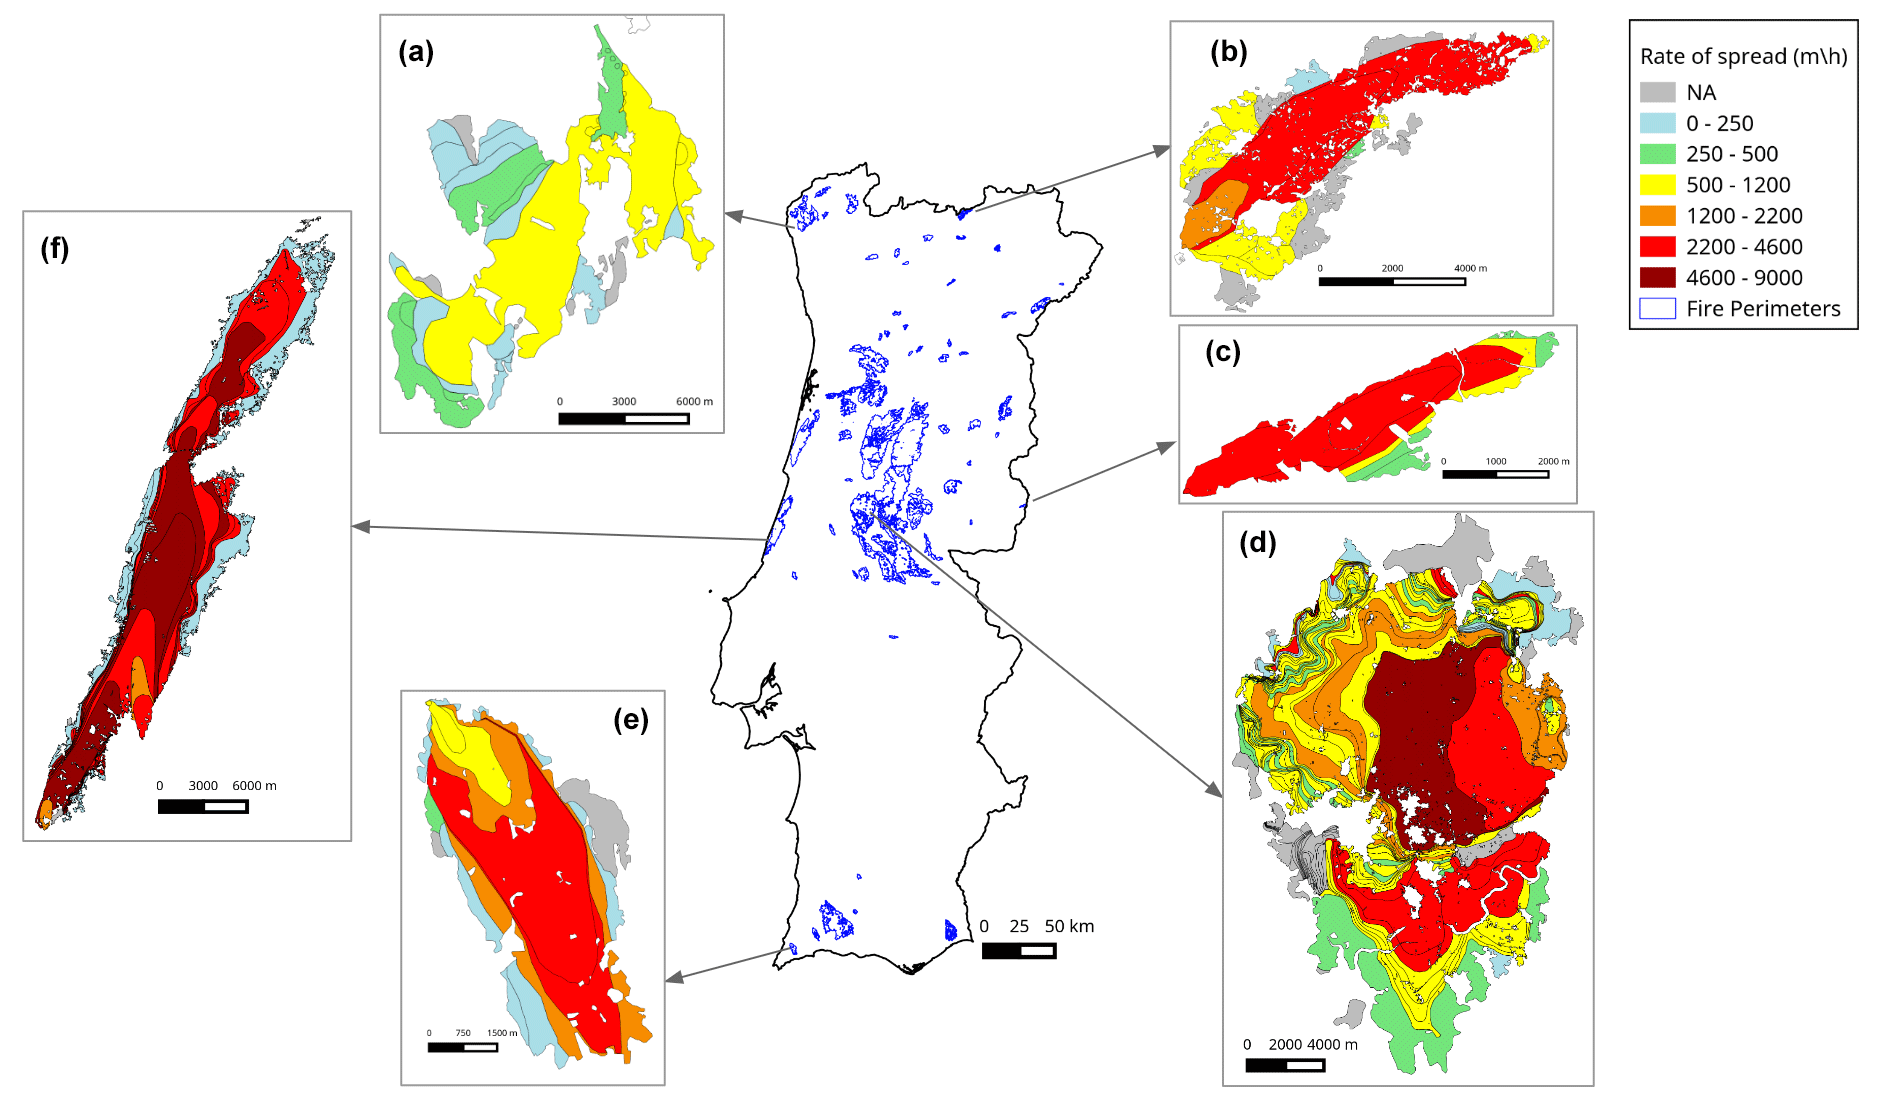
\includegraphics[width=1\linewidth]{images/Overall_spatial_distribution_of_wildfire_perimeters_in_Pt.png}
    \caption{\footnotesize{The distribution of wildfires in Portugal was analyzed using the Pt-FireSprd database project between 2016-2020.\cite{benali2023ptfiresprd} The perimeters show an analysis of the fire rate of spread (ROS) for six wildfires: (a) Paredes de Coura (2016), (b) Chaves (2020), (c) Idanha-a-Nova (2020), (d) Pedrógo Grande (2017), (e) Aljezur (2020), and (f) Alcobaça (2017).}}
    \label{fig:distribution_wildfire_rate_of_spread}
\end{figure}


\begin{figure}[H]
    \centering
    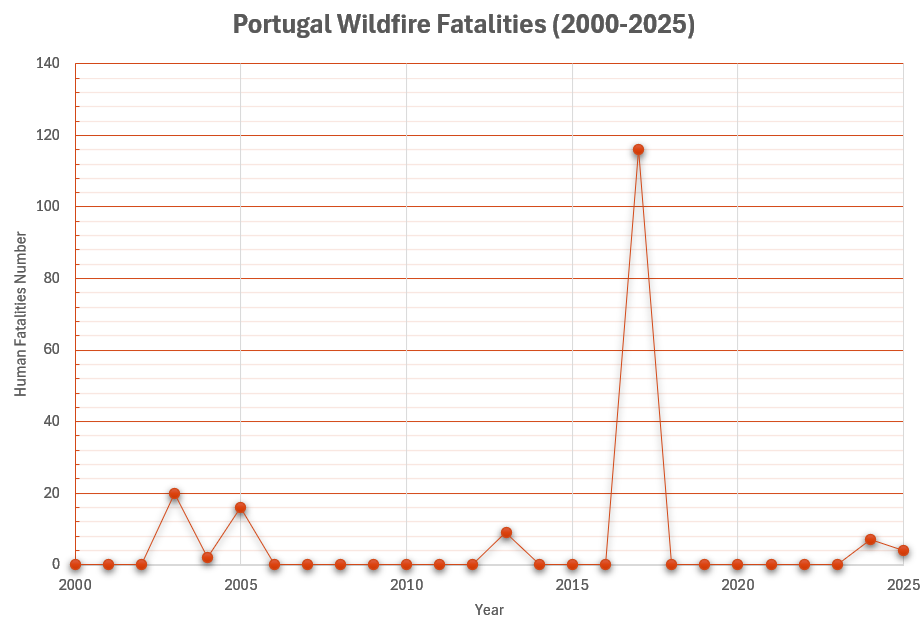
\includegraphics[width=0.75\linewidth]{images/wildfire_fatalities_pt.png}
    \caption{\footnotesize{Annual wildfire fatalities in Portugal (2000–2025). Key values from CTI reports for 2017 \cite{CTI2017_June,CTI2018_October}, MAI (2013) \cite{MAI2013_Accidents}, Viegas (2009) and Rodrigues et al. (2022) for 2003/2005 \cite{Viegas2009_CercadosParteII,Rodrigues2022_RuralFiresLosses}, and AGIF for 2023 \cite{AGIF2024_SGIFR2023}; 2024–2025 are provisional \cite{Reuters2024_PortugalWildfires,ECHO2025_PortugalFiresFlash}.}}
    \label{fig:pt_wildfire_fatalities}
\end{figure}
\footnotetext{Reproduced from Abatzoglou, J.~T., Williams, A.~P., \& Barbero, R. (2019), \textit{Geophys. Res. Lett.} 46, 326–336, doi:10.1029/2018GL080959. 
\copyright~2019 American Geophysical Union.\cite{effisPRTstats}}


% \vspace{1.5em}
\subsection{Need for strengthening the current Portuguese Earth Observation Capabilities for wildfire managemen}

Spaceborne assets are invaluable but split between \emph{coarse, frequent geostationary} views and
\emph{finer, infrequent polar} passes; performance can degrade under smoke/cloud, and \emph{small/fast ignitions are often detected late}, limiting time-to-first-intervention and model fidelity
\cite{wooster2021review}. Portugal has an integrated wildfire management system 
involving multiple agencies under the Agência para a Gestão Integrada de Fogos Rurais 
(Agency for Integrated Rural Fire Management, AGIF). 
AGIF sets the national policies and strategies for wildfire prevention and control.

Besides ground sensors, AGIS’s fire combat system uses typical satellite imagery 
like \emph{Sentinel-2}, which has a \emph{nominal 5-day revisit} to the same Earth’s region of 
interest, in other words, \emph{5 days of temporal resolution}\cite{esa_s2_facts}. 
This doesn’t match the hourly-scale dynamics of ignition and early spread.

% \vspace{1.5em}
\subsection{Low-fidelity Fire Weather Prediction}

Within the \emph{ImFire} project at the \emph{Association for the Development of Industrial Aerodynamics} (Associação para o Desenvolvimento da Aerodinâmica Industrial, ADAI), the workflow runs fire-spread models to forecast behavior and likely propagation corridors\cite{pereira_metaheuristic_2024}. However, in practice, these models rarely directly use satellite images for ignition location or active fireline geolocation because available EO streams usually lack the necessary temporal cadence and/or spatial detail for hour-scale operations (e.g., Sentinel-2’s roughly 5-day revisit). Therefore, ImFire mainly depends on meteorology, fuels, topography, and operational reports from ground sensors or aircraft, while satellite data are more often used for situational awareness or post-event mapping than for real-time model input.

% \vspace{1.5em}
\subsection{New Faster Constellation Requirements}

The performance of an alert system earth observation satellite constellation is mostly defined by two parameters: the time interval between consecutive passes of one spacecraft over the same Earth spot, defined as \textbf{temporal resolution} $\Delta t$ or $t_{\text{revisit}}$, and the space platforms imaging capability to resolve the ground scene from the spacecraft's perspective, defined as \textbf{spatial resolution $\Delta s$ or Ground Sample Distance (GSD)}. 

A dedicated satellite constellation could offer the requisite high temporal and spatial resolution, exceeding existing capabilities in fire weather forecasting. The ImFire team is collaborating with this thesis and has proposed a set of requirements to better suit their models. They have indicated that a \textit{satellite constellation} with a \textbf{temporal resolution $\mathbf{{t_{revisit} \approx 30}}$} minutes and a \textbf{spatial resolution\textbf{ }$\mathbf{{GSD \approx 6 \text{ \textbf{m/pixel}}}}$  }would \textit{significantly improve the accuracy of fire model predictions}\inlineReq{R7}, \inlineReq{R8},
\cite{ipcc2023syr,pereira2024fire,benali2023ptfiresprd}.

Figure \ref{fig:gap_satellite_constellations_spatial_temporal_plot} shows the gap in the know state of the art of low Earth orbit satellite constellations for fire detection. The target for this thesis, the Constellation Satellite $\mathcal{C}_{\text{sat}}$ design, is plotted at a temporal resolution of approximately 30 minutes and a spatial resolution of around 6 meters per pixel, which lies beyond the existing performance frontier and motivates the orbital architecture developed in this work.

\begin{figure}[H]
    \centering
    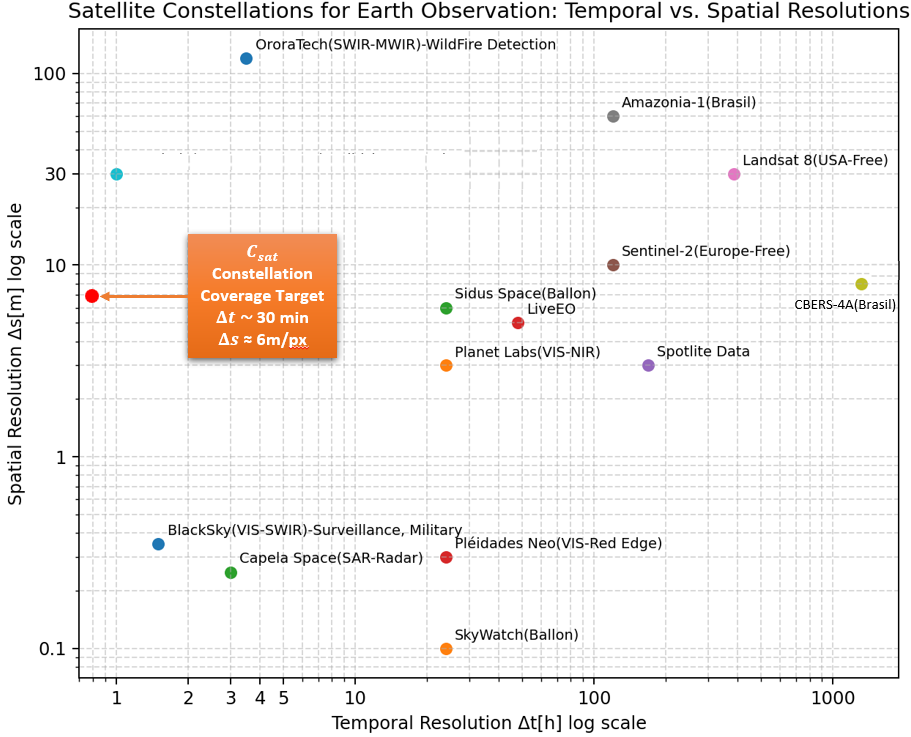
\includegraphics[width=1\linewidth]{images/satellite_constellations_spatial_temporal_plot.png}
    \caption{\footnotesize{Spatial resolution (GSD) vs.\ temporal resolution (revisit time) for known LEO satellites and constellations capable of fire detection. Mission target $\mathcal{C}_{\text{sat}}$.}}
    \label{fig:gap_satellite_constellations_spatial_temporal_plot}
\end{figure}


\begin{tcolorbox}[colback=white, colframe=black, title=\textbf{Problem Statement}]
\emph{Wildfire risk in Mediterranean Europe}---including Portugal---has intensified under the Great Acceleration \cite{steffen2015trajectory}, with projections indicating significant \emph{rises in fire weather}, \emph{longer seasons}, and \emph{larger burned area across Iberia} \cite{ipcc2023syr,jolly2015climate, pereira2024fire, benali2023ptfiresprd}. Catastrophic episodes such as \emph{Pedrógão Grande (2017)} show how, under extreme \emph{pyrometeorology}, \emph{fire fronts can accelerate and overwhelm decision windows}---and that \emph{near--real-time orbital detection/nowcasting was not integrated into operations} at the time \cite{cti2017pedrogao}. Current satellite services face a \emph{resolution--revisit--latency gap}: \emph{coarse/frequent GEO} plus \emph{finer/infrequent LEO} often \emph{miss or delay} small, fast-moving ignitions and \emph{degrade under smoke/cloud}, constraining timely intervention and model fidelity \cite{wooster2021review,esa_s2_facts}. Moreover, \emph{Portuguese fire-prediction workflows} depend on Sentinel 2 inputs whose \emph{temporal cadence} of 5 days and spatial resolution for the fire prediction application of $30 \text{m/px}$ is insufficient for hour-scale dynamics; improving forecast capabilities requires \emph{high-frequency, high-resolution} EO data \cite{pereira_metaheuristic_2024}. 

\vspace{1em}
\textbf{Scientific problem:} a mismatch between \emph{the temporal/spatial scale of fire dynamics} and the \emph{capability of existing orbital observation systems for fire management}---which raises the central research question: \emph{what satellite constellation design can close this spatiotemporal gap, improving fire-weather and fire-spread prediction for Portugal?}
\end{tcolorbox}


\section{Aim and Scope}\label{sec:aim-and-scope}

\begin{tcolorbox}[colback=white, colframe=black, title=\textbf{Aim}\label{aim}]
To design an \emph{orbital architecture} for a small-satellite constellation that enables \emph{minute-scale revisit ($\approx$30 min), meter-scale detail (\textasciitilde6 m GSD), day/night and all-weather	visibility, and low end-to-end latency} over \emph{continental Portugal}, sufficient to \emph{improve fire-weather and fire-spread model inputs} and \emph{support tactical decision-making}, and to analyze the coverage reach of the proposed constellation over regional and global fire-prone regions.
\end{tcolorbox}

\emph{Scope}\label{scope}

What this work will cover and not cover?
\vspace{1.5em}

\emph{In scope:}

\begin{itemize}
	\item
	      \textbf{Orbital architecture design:} High-fidelity mission simulation using  GMAT and Orekit to analyze Kepler parameters, altitude/inclination selection, comparison between Sun Synchronous Orbit and Repeating Ground Track Orbit, non-resonant orbits, plane count and spacing, single vs. multi-layer constellations, and phase management.
	\item
	      \textbf{Coverage \& performance analysis:} access time, mean/worst-case revisit, probability of access within operational windows, geometry needed to achieve target GSD over Portugal; seasonal/diurnal effects, groundtrack coverage.
	\item
	      \textbf{Sensitivity studies:} number of satellites, altitude, RAAN
	      spacing, temporal coverage maps; trade-offs among revisit, GSD, and
	      latency.
	\item
	      \textbf{Implications for sensing (high level only, optional time dependent):} derive
	      \emph{top-level sensor family requirements} implied by the chosen
	      architecture (e.g., optical/thermal/microwave, day/night/all-weather),
	      \emph{without} detailed payload design.
        \item
          \textbf{Communications \& latency budgets(optional, time dependent):}
          inter-satellite links vs. direct-to-ground, ground-station network
          options, onboard vs. ground processing assumptions,
          \emph{detection-to-decision} timing analysis.
\end{itemize}

\emph{Out of scope:}

\begin{itemize}
	\item
	      \textbf{Detailed payload engineering:} detector/optics/radiometry
	      design, SNR/NE$\Delta$T budgeting, thermal/power/mechanical design,
	      calibration/validation plans.
	\item
	      \textbf{Algorithm development:} new fire-detection or spread-model
	      algorithms beyond using published performance assumptions for
	      cadence/latency needs.
	\item
	      \textbf{Operational coupling at a high level:} mapping cadence/latency
	      to \emph{model-update frequency} and
	      \emph{time-to-first-intervention}; conceptual interfaces with
	      existing Portuguese workflows (e.g., AGIF/ImFire).
	\item
	      \textbf{Programmatics/economics:} cost models, procurement,
	      regulatory/licensing and spectrum coordination.
	\item
	      \textbf{Full operational integration \& field deployment:} end-to-end
	      real-world trials or system acquisition; global designs beyond
	      Portugal (except brief generalization notes).
\end{itemize}


\section{Significance of the Study}\label{sec:significance}

This work addresses a documented gap in the fire-detection state of the art: no existing or planned satellite constellation combines sub-hour revisit with metre-scale ground resolution over fire-prone regions.
The orbital architecture and design methodology developed here provide a transferable framework for closing that gap---first for Portugal, then for any fire-prone latitude worldwide.

\section{Structure of the Thesis}\label{sec:structure}

This thesis follows a NASA/ESA systems-engineering life-cycle scoped to Pre-Phase~A and Phase~A (the full methodological framework is detailed in Appendix~\ref{app:se_approach}). The narrative moves from evidence $\rightarrow$ needs $\rightarrow$ concepts $\rightarrow$ simulation trades $\rightarrow$ baseline solution, organised in three parts.


\begin{figure}[H]
	\centering
	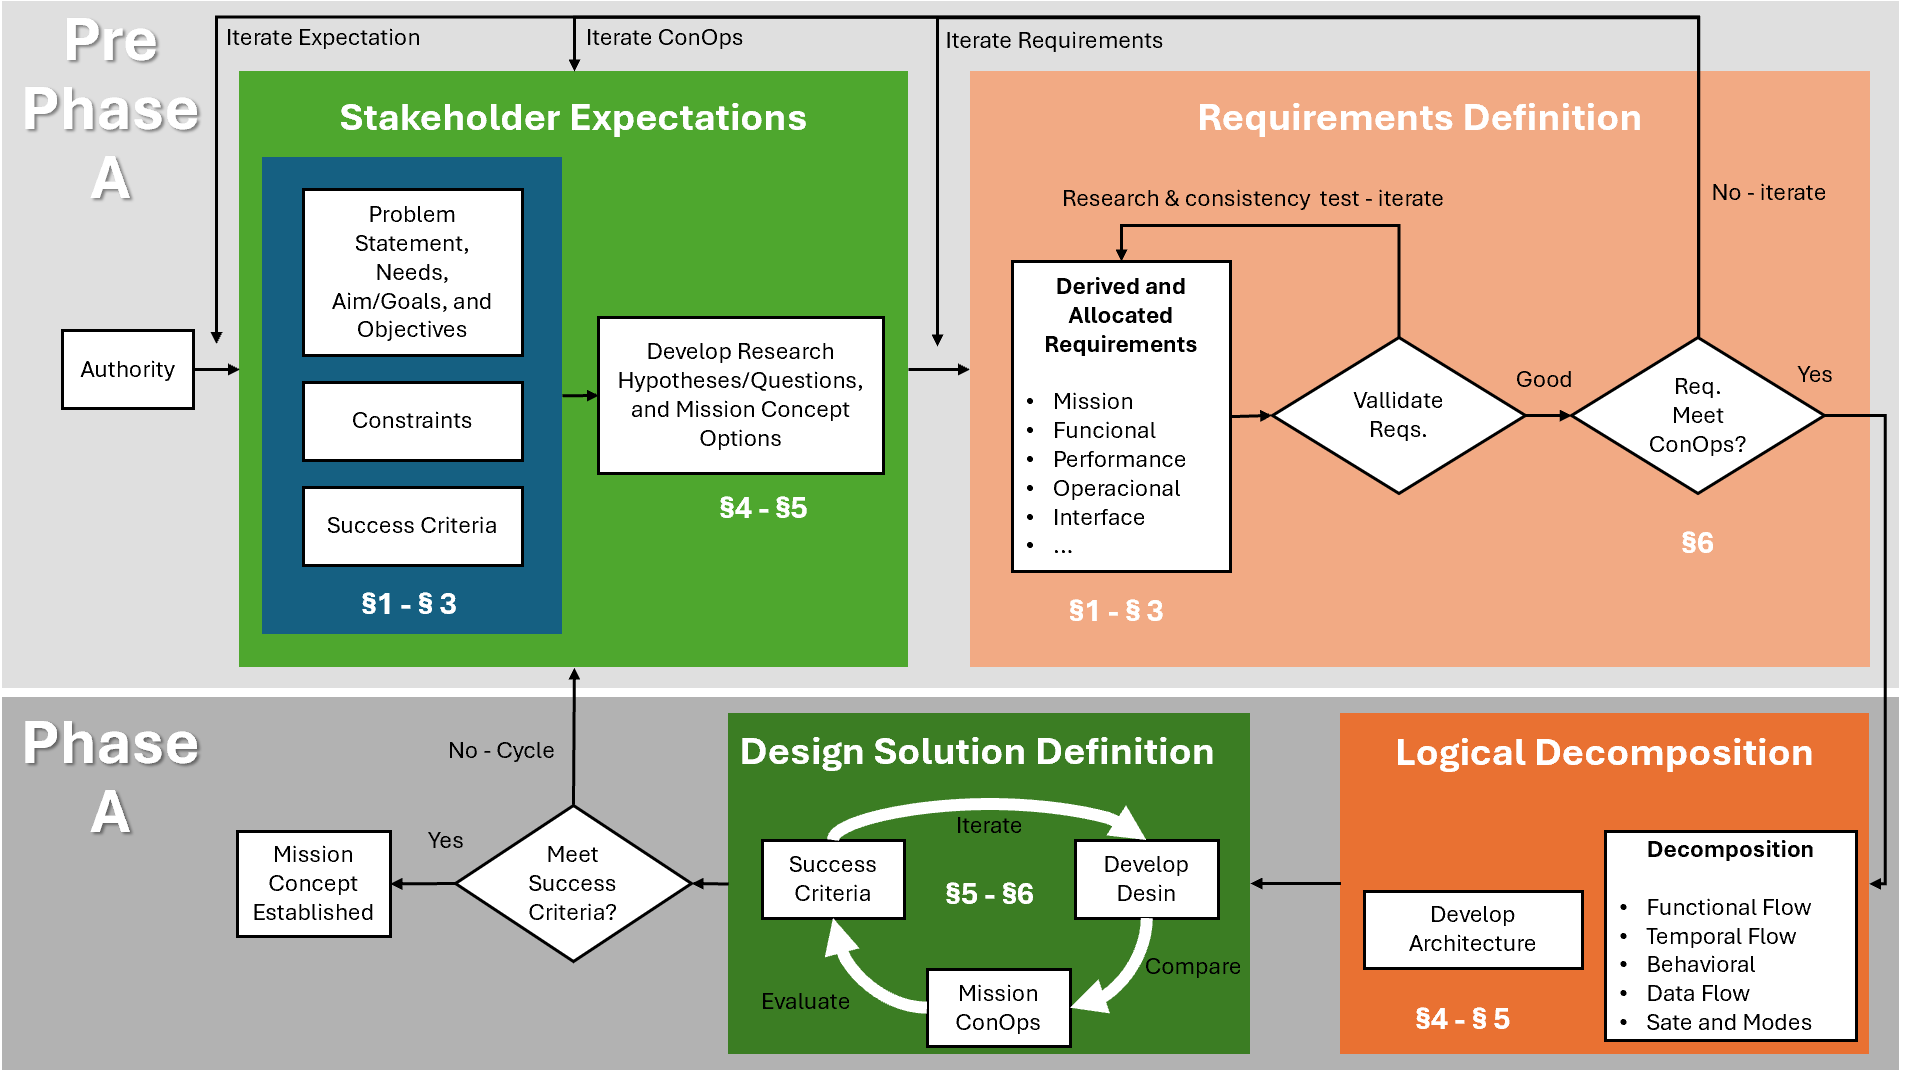
\includegraphics[width=1\textwidth]{images/c1.4.2_Interrelationships_SE_PrePhase_A_Phase_A.png}
	\caption[Connections between Pre-Phase A and Phase A system design processes. The chapters where these processes are discussed are highlighted with the symbol \S. Adapted from]{Relation between Pre-Phase A and Phase A system design processes. The chapters where these processes are discussed are highlighted with the symbol \S. Note the Stakeholder Expectation and Requirements Definitions overlap in chapter \S1 - \S5. Adapted from \parencite{SEHandbook}.}
	\label{fig:nasa-lifecycle_prephaseA-phaseA}
\end{figure}


PART I (Chs. 1--3) establishes the problem context, study domains, and physical foundations (Pre-Phase A). 
Chapter 1 states the context, motivation, aim, and scope, framing the spatiotemporal observation gap that motivates the thesis. 
Chapter 2 defines the Core Study Domain ($\mathcal{D}_{core}$, mainland Portugal) and Global Study Domain ($\mathcal{D}_{global}$, Earth's fire-prone regions), establishing spatial, temporal, and reference-data boundaries. 
Chapter 3 develops the radiometric and geometric physics of fire remote sensing from orbit, deriving the observation constraints that drive sensor and constellation requirements. 

PART II (Chs. 4--5) starts Phase A with theory and architecture trade-offs. 
Chapter 4 presents the constellation-design fundamentals: observation formalism, orbital mechanics, visibility geometry, and Repeating Ground Track Orbit theory, including a quantitative comparison with Sun-Synchronous Orbits that justifies the RGTO selection. 
Chapter 5 explores the Walker RGTO design space, selects seed orbital parameters, and defines the plane count and satellite phasing to satisfy the revisit requirements over Portugal. 

PART III (Chs. 6--8) presents and interprets outcomes. 
Chapter 6 synthesises the results of the baseline 15-satellite constellation and the two-layer Watcher--Zoom tip-and-cue architecture. 
Chapter 7 discusses feasibility, limitations, and transferability of the results, 
and Chapter 8 concludes by answering the research questions and outlining avenues for future work. 

Six appendices provide supporting derivations and data: the geopotential $J_2$ model (A), the SSO-vs-RGTO benchmark (B), station-keeping and orbit lifetime (C), Walker RGTO element tables (D), the consolidated requirements list R1--R25 (E), and the full systems-engineering methodological framework (F).


\section{Requirement Mission Objectives and Level-1 Summary}\label{sec:requirements_level1}

This subchapter presents the chapter 1 insights as mission requirements, formatted in a systems engineering style. It provides a complete description of mission needs. The table below supports traceability and reference for theory, methodology, simulation constraints, and expected results.

\vspace{\baselineskip}
Requirement table symbolism legend:
\vspace{\baselineskip}

\requirement{R\#}{Requirement Name}{Description of the requirement.}{Req. type}{Subsystem/Parameter/Tag}
\vspace{\baselineskip}


\vspace{\baselineskip}
The complete definition of the mission objectives (R1--R4), environmental constraints (R5), and constellation performance requirements (R6--R8) is provided in Appendix~\ref{sec:app_req_ch1}.


% --- CHAPTER 2: The Wildfire Challenge and Study Case Definition: From Global Threat to Local Data Needs ---
\chapter{\texorpdfstring{The Wildfire Challenge and Study
Case Definition: From Global Threat to Local Data Needs
}{The Wildfire Challenge and Study Case Definition: From Global Threat to Local Data Needs }}\label{chapter-2-the-wildfire-challenge-and-study-case-definition-from-global-threat-to-local-data-needs}

% \begin{quote}
% \textbf{Writing Guide \& Methodological Focus:}

% \begin{itemize}
% \item
%   \textbf{Objective:} To convince the reader with detailed literature
%   review that wildfires are a severe and escalating problem demanding a
%   better solution. This chapter establishes the "why" of the thesis.
%   Also it indicates what is the target object of the constellation,
%   Study Area, Study Period, and Event Set (AOI/ROIs \& Cases):
% \item
%   \textbf{Method:} Start with the global context and then funnel down to
%   the specific, acute problem in Portugal. Use strong data and
%   references to build this research study case.
% \item
%   \textbf{Caution:} Focus on the \emph{problem} and its \emph{impact}
%   and narrow to the thesis study case. Do not discuss satellite
%   solutions in detail yet neither ecology of wildfire in detail, only
%   enough to get spatial and temporal data
% \item
%   \textbf{Checkpoint:} Has this chapter clearly established that
%   Portugal has a critical, unsolved wildfire problem that justifies a
%   new technological solution and that the critical spatial temporal
%   periods of the constellation have stabilized?
% \end{itemize}
% \end{quote}
% This chapter aims to define the satellite constellation's object of study, which is the wildfire-burning biomass on the planet's surface as seen from an orbiting satellite. We want to answer the questions of where on the planet the satellite shall observe, why this spot on Earth is particularly important, and when the spacecraft must focus its attention on this region. 

% To answer these questions, a literature review is conducted on the the historical emergence of Anthropocenic-induced wildfires, their evolution on a global scale, and their predicted future impacts. The analysis is carried out from the perspective of two key metrics: one that \textit{quantifies fire danger}, known as the \textbf{Fire Weather Index (FWI)}, and another that \textit{measures fire damage} in a region, referred to as the \textbf{Burned Area (BA)}.  From the historical FWI and BA maps and trends analysis, the primary and secondary \textbf{Areas of Interest (AOI)} are derived. Each region has a \textbf{Time of Interest (TOI)} defined by the pattern of the region's fire season.



% \section{\texorpdfstring{Global Fire Atlas - Past, Present, and Future
% }{Global Fire Atlas - Past, Present, and Future}}\label{21-global-wildfire-atlas-------hotspots-and-stats}

% This section provides information on climate change science to help understand how human actions have affected fire activity on the planet past, the current wildfire activity crisis, and the difficult challenges ahead. 

% \subsection{Anthropocene impact on Fire Weather Index}

% The Anthropocene is an era where human forces affect the dynamics of biospherical, climate, and geological systems.  This era has an inflection point called the Great Acceleration, which occurred in the mid-20th century, around 1950 . During this time, anthropogenic forces amplify, showing their transformative and disruptive impacts, sharply increasing pressures on climate and ecosystems, and framing today's wildfire risks within rapid Earth-system changes. \cite{steffen2015trajectory} \cite{abatzoglou_global_2019}. 

% Figures \ref{fig:socio_economic_and_earth_system_trends} and \ref{fig:anthropogenic_climate_change_emergency_fire_index} connect socio-economic and earth system trends of the Anthropocene Great Acceleration with increased global wildfire activities.
% Analyzing both figures, it is possible to observe that the socio-economic growth trends match two patterns: First)\textbf{Reduced Fire Resilience in Earth Systems} embodied as increases in atmospheric CO\textsubscript{2}, temperature, tropical forest loss, domesticated land use, and biosphere degradation which combined increase fire activity (biosphere and atmospheric damage \rightarrow  more fuels in drier conditions \rightarrow more ignitions); Second)\textbf{Increase of Fire Weather Index(FWI) linked to Antropogenic Climate Change} which is shown as Time of Emergence (ToE) of altered fire weather in subcontinental regions. 
% Next, we will analyze the global trend of FWI.





% \begin{figure}[H]
%     \centering
%     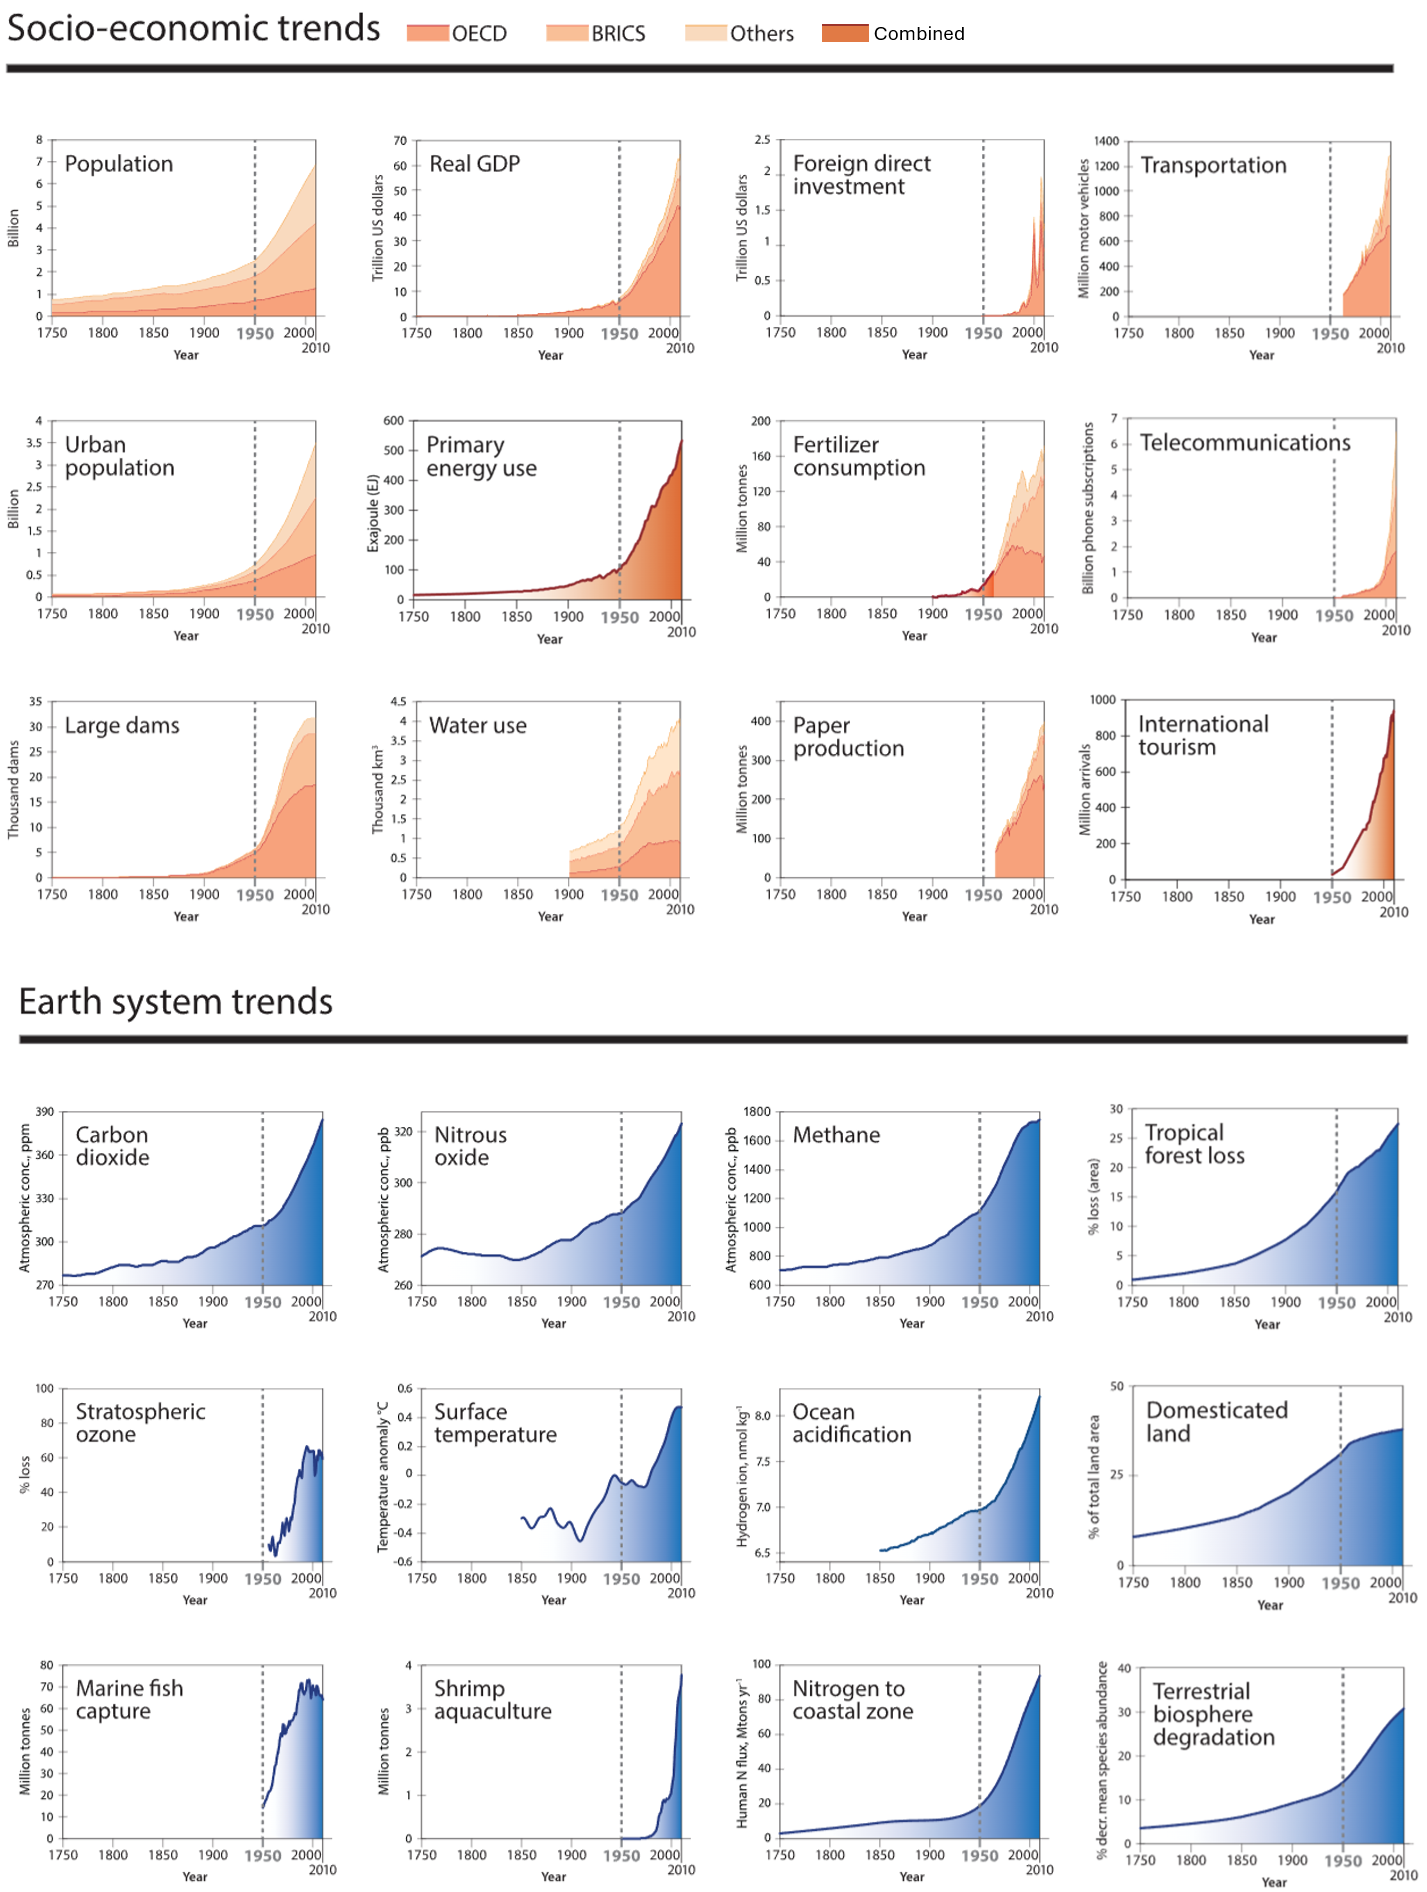
\includegraphics[width=0.97\linewidth]{images/socio_economic_and_earth_system_trends.png}
%     \caption{\small{The Great Acceleration (1750–2010), compact view after Steffen et\,al.\ (2015) \cite{steffen2015trajectory}.  Top: Global socio-economic trends split by OECD, BRICS, and the rest, accelerated post-1950 with sharp growth in population, energy, transport, fertilizer, water, and telecommunications. Bottom: Earth-system trends show increases in atmospheric CO\textsubscript{2}, temperature, tropical forest loss, domesticated land use, ocean acidification, and biosphere degradation. These pathways reduce fire resilience and increase wildfire risk through deforestation, biosphere and atmospheric damage, drier conditions, more fuels, and ignitions. Figure \ref{fig:anthropogenic_climate_change_emergency_fire_index}  links this post-1950 shift to observed and projected increases in global fire weather index.}}
%     \label{fig:socio_economic_and_earth_system_trends}
% \end{figure}


% \begin{figure}[H]
%     \centering
%     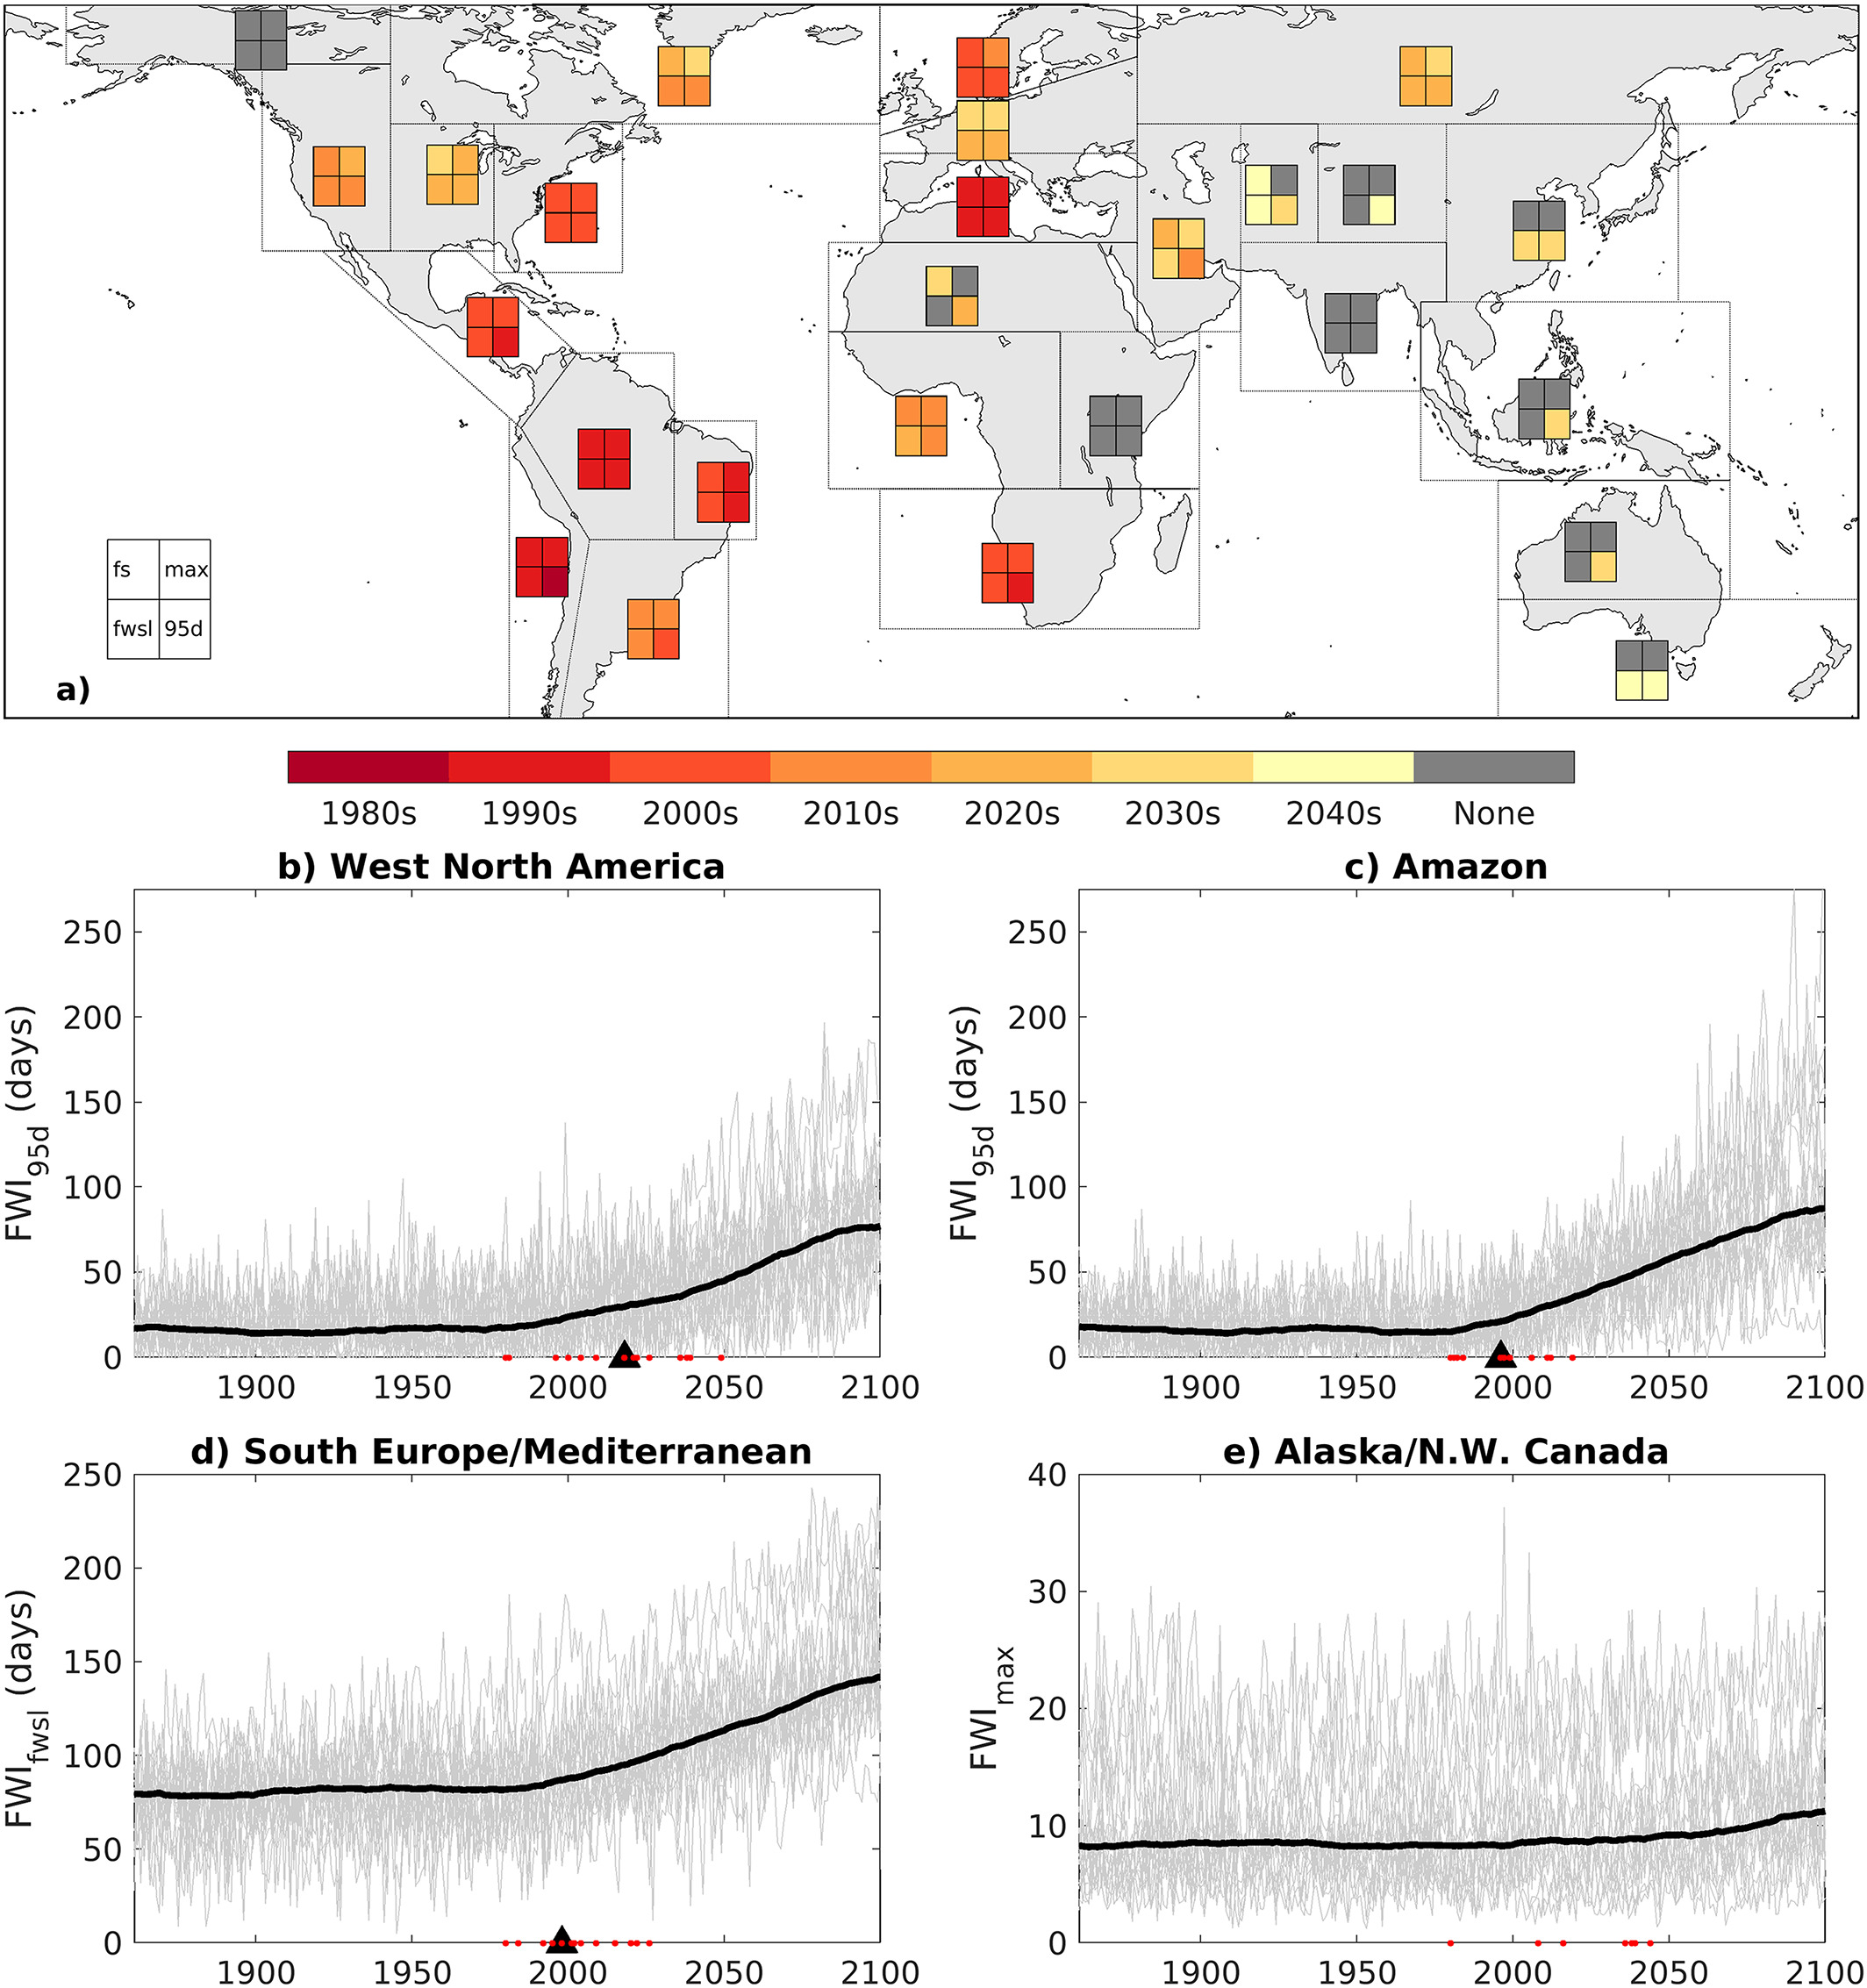
\includegraphics[width=0.95\linewidth]{images/anthropogenic_climate_change_emergency_fire_index.png}

%     \caption{\footnotesize{Time of emergence (ToE) of anthropogenic climate change in Fire Weather Index (FWI) metrics across subcontinental regions.
%     (a) Median ToE from 17 models between (1980-2040); each regional tile shows four metrics by quadrant:
%     95d = FWI$_{95\mathrm{d}}$ (frequency of extreme days),
%     fwsl = FWI$_{\mathrm{fwsl}}$ (season length),
%     fs = FWI$_{\mathrm{fs}}$ (peak 90-day mean),
%     max = FWI$_{\max}$ (annual maximum).
%     Time series between 1861-2100 for selected regions:
%     (b) FWI$_{95\mathrm{d}}$—West North America;
%     (c) FWI$_{95\mathrm{d}}$—Amazon;
%     (d) FWI$_{\mathrm{fwsl}}$—South Europe/Mediterranean;
%     (e) FWI$_{\max}$—Alaska–Northwest Canada.
%     Bold black line: 30-year multimodel median; red dots: each model ToE; black triangle: 17-model median ToE where at least nine models show emergence.
%     \protect\footnotemark}}
%     \label{fig:anthropogenic_climate_change_emergency_fire_index}
% \end{figure}

% \footnotetext{\label{fn:abatzoglou2019}\footnotesize{Reproduced from Abatzoglou, J.~T., Williams, A.~P., \& Barbero, R. (2019), \textit{Geophys. Res. Lett.} 46, 326–336, doi:10.1029/2018GL080959. 
% \copyright~2019 American Geophysical Union.\cite{abatzoglou_global_2019}}}

% \begin{figure}[H]
%     \centering
%     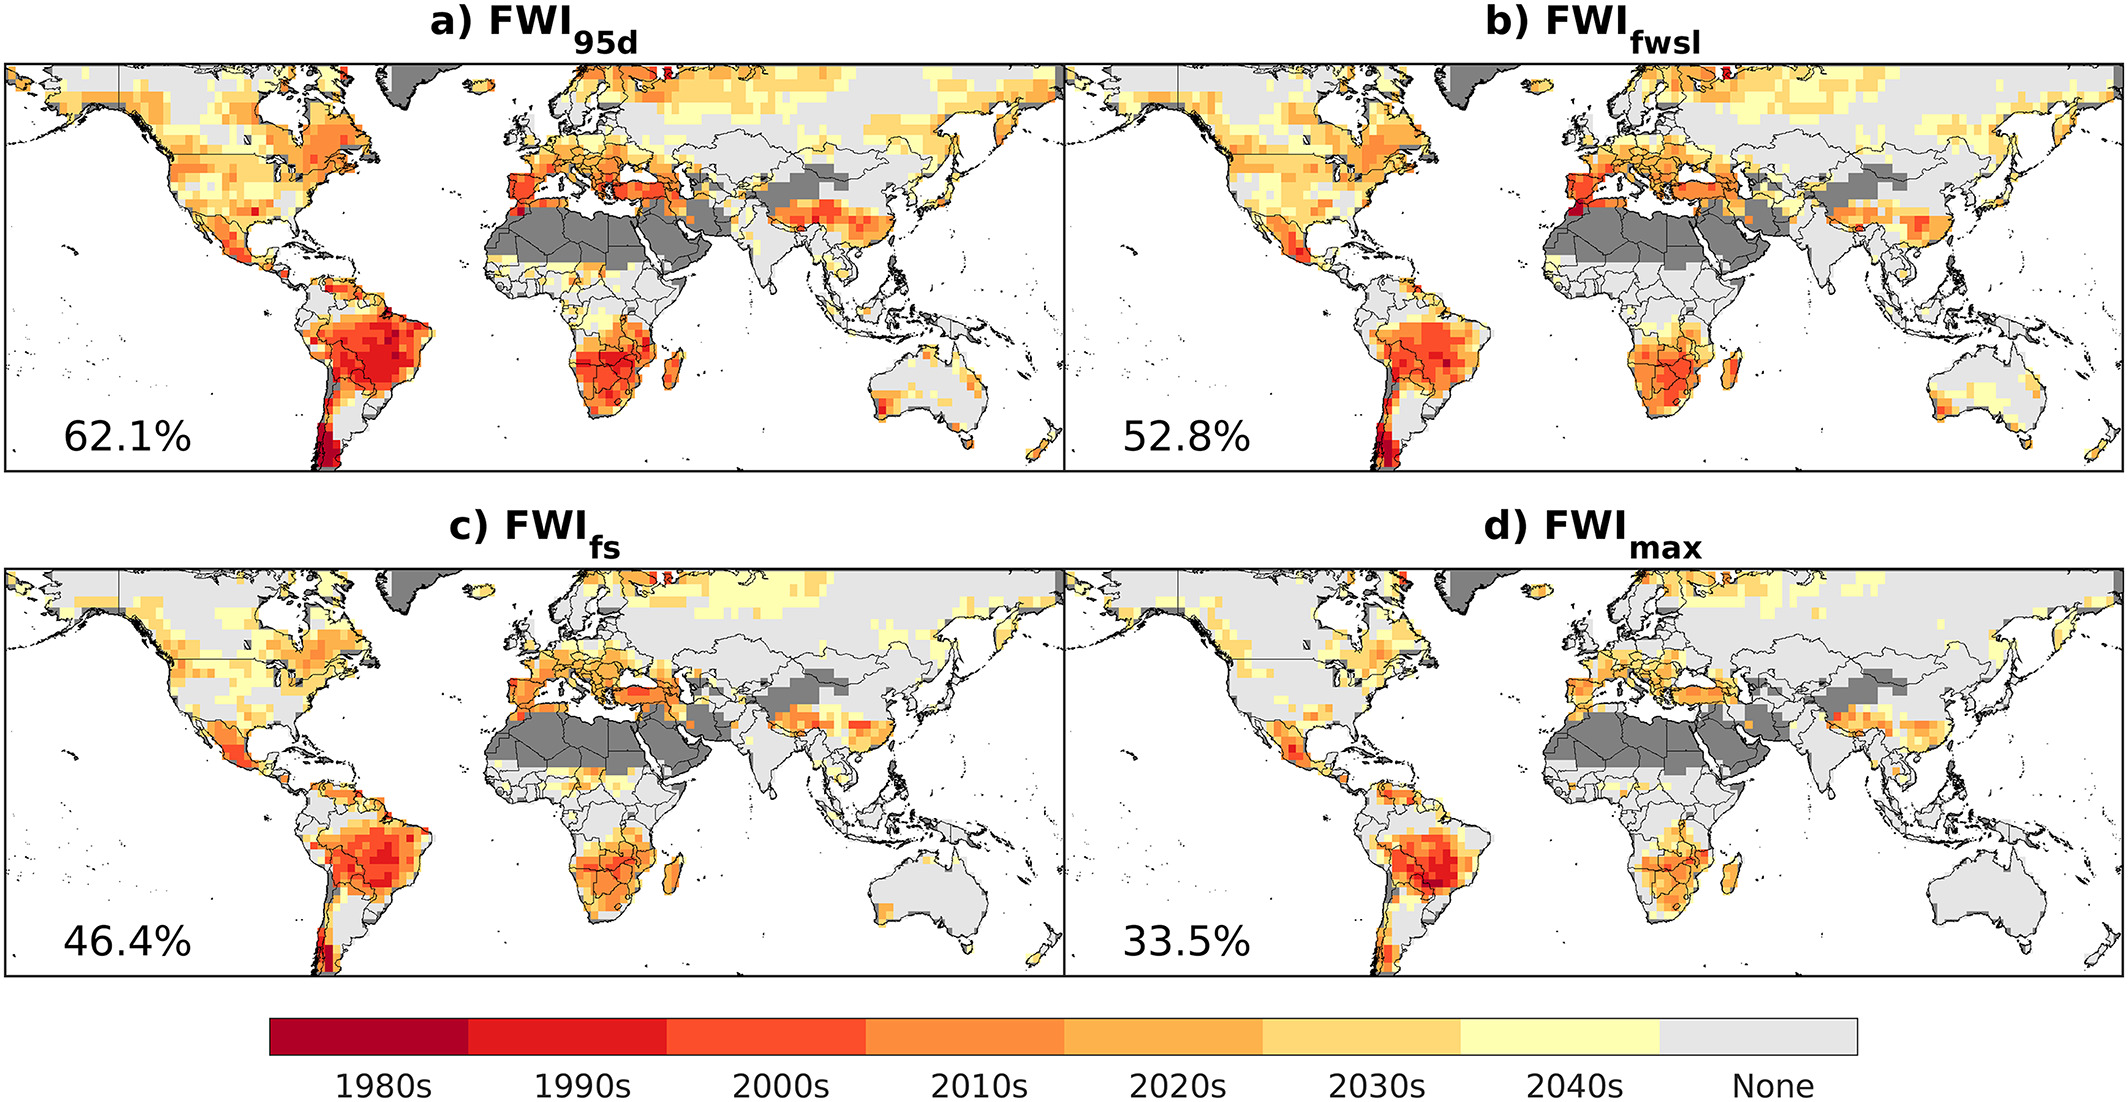
\includegraphics[width=1\linewidth]{images/fire_anthropogenic_ToE_detailled.png}
%     \caption{Time of emergence of anthropogenic climate change for (a) the frequency of days exceeding the 95th percentile (extreme fire days \( \mathrm{FWI}_{\mathrm{95d}} \)), (b) the length of the fire weather season (\( \mathrm{FWSL} \)),(c) the peak 90-day average (FWI$_{\max}$), and (d) annual maximum (\( \mathrm{FWI}_{\mathrm{fs}} \)). Mapped is the 17-model median date at which the anthropogenic signal emerges based on the change exceeding the standard deviation of the baseline period. Areas of light gray highlight where the signal does not emerge for at least eight models by 2050. Unburnable lands where >80\% of the area is water, snow, and ice, or barren or sparsely vegetated, are shown in dark gray. The percent of burnable land with emergence by 2050 is denoted in the bottom left corner of each map.\textsuperscript{\ref{fn:abatzoglou2019}}}
%     \label{fig:anthropogenic_climate_change_emergency_fire_index_detailled}
% \end{figure}

% \subsection{Global Rise of the Fire Weather Index(FWI)}

% Building on climate-model simulations, Abatzoglou et al. (2019) estimate the time at which anthropogenic forcing makes fire-weather indices exceed the range expected from natural variability at subcontinental scales\cite{abatzoglou_global_2019}. Figure \ref{fig:anthropogenic_climate_change_emergency_fire_index}  shows the Time of Emergence (ToE) of anthropogenic climate change in subcontinental regions. 

% The metric used to analyze wildfire risk is the Fire Weather Index (FWI). The FWI is a unidimensional unit that measures the likelihood of fire intensity based on fuel dryness and fire weather, regardless of the type of biomass covering the land. The inputs needed to calculate the FWI are daily temperature, humidity, wind speed, and accumulated rainfall. FWI is explained in more detail in chapter \ref{31-the-fire-itself-physics-of-the-radiative-signature}. The main quantities necessary to understand the fire weather properties used on Figure \ref{fig:anthropogenic_climate_change_emergency_fire_index}- \ref{fig:map_FWSL_FWI95d_change_relative_1979_2019} are summarized in Table \ref{tab:fwi_metrics}.(TODO: Replace table with a drawing of FWI curves connecing the FWI curves and burned areas and fire frequency)

% %\begin{itemize}
% %  \item \textbf{FWI95d (frequency of extreme days).} Number of days per year when daily FWI exceeds the local 95th-percentile threshold defined from a historical baseline; indicates how often “very bad” fire-weather occurs.
% %  \item \textbf{FWIfwsl (fire-weather season length).} Days per year with FWI above the mid-range point (average of the local baseline maximum and minimum FWI); indicates how long conditions remain conducive to fire spread.
% %  \item \textbf{FWIfs (seasonal peak 90-day severity).} Highest 90-day running mean FWI within the year; captures the intensity of the core fire season regardless of its timing.
% %  \item \textbf{FWImax (annual daily maximum).} Single highest daily FWI in the year; a magnitude-of-extremes metric related to the potential for extreme runs/spread.
% %\end{itemize}


% \begin{table}[h]
% \centering
% \footnotesize
% \begin{tabularx}{\textwidth}{|l|l|X|}
% \hline
% \textbf{Symbol} & \textbf{Meaning} & \textbf{Description} \\
% \hline
% $\mathrm{FWI}$ & Fire weather index & 
% Unitless composite from daily max temperature, min relative humidity, 24\,h precipitation, and mean wind speed; combines fuel-moisture buildup and wind-driven spread. \\
% \hline
% $\mathrm{FWI}_{95\mathrm{d}}$ & Extreme days per year & 
% Number of days in a year when daily FWI exceeds the local 95th-percentile threshold (threshold from a historical baseline). \\
% \hline
% $\mathrm{FWI}_{\mathrm{fwsl}}$ & Season length & 
% Days per year with FWI above the mid-range point (average of the local baseline maximum and minimum FWI). \\
% \hline
% $\mathrm{FWI}_{\mathrm{fs}}$ & Peak 90-day severity & 
% Highest 90-day running mean FWI within the year (sliding window), capturing core-season intensity regardless of timing. \\
% \hline
% $\mathrm{FWI}_{\max}$ & Annual maximum & 
% Maximum daily FWI observed in the year (single-day extremity). \\
% \hline
% \end{tabularx}
% \caption{Fire Weather Index (FWI) metrics used in wildfire risk assessment}
% \label{tab:fwi_metrics}
% \end{table}


% Abatzoglou et al.\cite{abatzoglou_global_2019} report that anthropogenic effects on fire weather index signals are detectable with increased amplitude in parts of southern Europe, West Noth America, South African Savannahs, the Amazon, and other regions. We can analyze the historical anthropogenic FWI effect by verifying the high-level Figure \ref{fig:anthropogenic_climate_change_emergency_fire_index}-a and the low-level detailed Figure \ref{fig:anthropogenic_climate_change_emergency_fire_index_detailled}. These plots show the Time of Emergence (ToE) of the anthropogenically induced FWI in different points for each sub-continent region. The earliest observable effect starts in the 80s, in the Peruvian Amazonian/Chile region. Between the 90s and 00s, we see a large emergent impact covering the Amazon, South Europe/Mediterranean, Northern Europe, Central America, Northeast and South Brazil, Argentina, the South African region, and Eastern North America. Later, between 10s-20s, human impact appears in Central and West North America, the North Canada/Greenland tundra region, central and north Africa, Western Asia, and Western and Eastern Europe. The prediction for anthropogenic fire activity impact extended between 30s-40s, where effects are seen in Western and Eastern Asia, South-eastern Asia, and Australasia. 

% Detailed trend of the fire weather season length \( \mathrm{FWSL} \)  and extreme fire days \( \mathrm{FWI}_{\mathrm{95d}} \) per region is seen in Fig \ref{fig:fire_season_FWSL_1979_2019} and Fig \ref{fig:fire_extreme_days_freq_FWSI95d_1979_2019}. Analyzing first the season length Fig \ref{fig:fire_season_FWSL_1979_2019},  in this plot, one can see that globally the fire season length increases from \(\sim\)60 days (2025) to \(\sim\)70 days (2050) and \(\sim\)78 days (2100). These values are a global average; however, it is important to note the regions where planetary frontiers can be crossed, and where human and biome life will be affected more severely and sooner. One region identified as a planetary tipping point that must keep fire weather under control to prevent a planetary critical transition is the Amazon. From Figure \ref{fig:fire_extreme_days_freq_FWSI95d_1979_2019} the Amazon extreme fire weather days per year \( \mathrm{FWI}_{\mathrm{95d}} \) goes from about 25 days in 2025 to approximately 50 days in 2050, and about 100 days in 2100. This increase in wildfire activities is likely linked to the deforestation–drought–fire feedbacks and could signify the savannization of the Amazonian biome, which aligns with tipping points and critical transitions. scenarios.(TODO:Mission requirement def, Secondary coverage, Amazon critical parts).\footnote{Rising fire-weather pressure in the Amazon interacts with deforestation–drought–fire feedbacks that may push parts of the biome toward "savannization." Multiple assessments place a tipping threshold near $\sim$20–25\% cumulative deforestation; The full Amazon forest basin loss has been reported at $\sim$17\% (and nearing 20\% in Brazil), showing the narrowing margin \cite{lovejoy_amazon_2019}. Regional research consortia warn this threshold could be approached in the 2025–2030 window under high-loss trajectories \cite{raisg_against_clock_2022}, while a recent \textit{Nature} synthesis projects that by $\sim$2050, 10–47\% of Amazon forests could face compounding disturbances capable of triggering local-to-regional transitions \cite{flores_critical_2024}. Within the Planetary Boundaries lens, these dynamics reflect interacting transgressions of land-system change and biosphere integrity, amplifying fire-weather risks \cite{richardson2023earth}.}

% Although impacts in the Amazon have planetary consequences in human population and biosphere/biodiversity, the most severe \textit{projected} increases in fire-weather exposure occur over southern Europe/the Mediterranean (Fig.~\ref{fig:anthropogenic_climate_change_emergency_fire_index}d), where the fire-season length metric \( \mathrm{FWSL} \) rises from \(\sim\)90 days (2025) to \(\sim\)120 days (2050) and \(\sim\)150 days (2100). Additionaly, Fig \ref{fig:fire_extreme_days_freq_FWSI95d_1979_2019} shows that the Mediterranean extreme fire days  \( \mathrm{FWI}_{\mathrm{95d}} \) increase from  \(\sim\)30 days (2025) to \(\sim\)45 days (2050) and \(\sim\)75 days (2100). Beyond wildfire meteorology, this region is a warming–aridification hotspot with large and dense connected wildland–urban interface and land-use legacies that amplify ignitions and losses. (TODO:Mission requirement def, Primary sub-continental region good for fast wildfire detection)(TODO: talk about the increase of death due to heatwaves)

% A planetary vision under the metric of the fire weather season length, which measured the impact of natural and anthropogenic causes of fire between 1979 and 2019, is projected onto the global map Fig \ref{fig:map_FWSL_FWI95d_change_relative_1979_2019}. 

% A planetary vision under the metric of the fire‐weather season length, which measured the impact of natural and anthropogenic causes of fire between 1979 and 2019, is projected onto the global map in Fig.~\ref{fig:map_FWSL_FWI95d_change_relative_1979_2019}. As analyzed by Jones et. al, on this plot, we see a synthesis of the trends under discussion; it's possible to see a crescent trend for the \( \mathrm{FSWL} \) and \( \mathrm{FWI}_{\mathrm{95d}} \). Also, as these metrics grow at different rates— in South America, Central Asia, and Africa, the increase in extreme days per year was greater than the expansion of the fire season length. On the other hand, in Europe and boreal Asia, the growth of the season was larger than the increase in extreme days.  The places with the earliest anthropogenic fire impact are the ones with the largest change in the relative fire season length, namely, Europe, central and boreal Asia, southern‐hemisphere South America, and temperate North America. Regarding the extreme fire days per year, the highest increase is in southern‐hemisphere South America, central Asia, and across Africa\cite{jones_global_2022}.

% \begin{figure}[H]
%     \centering
%     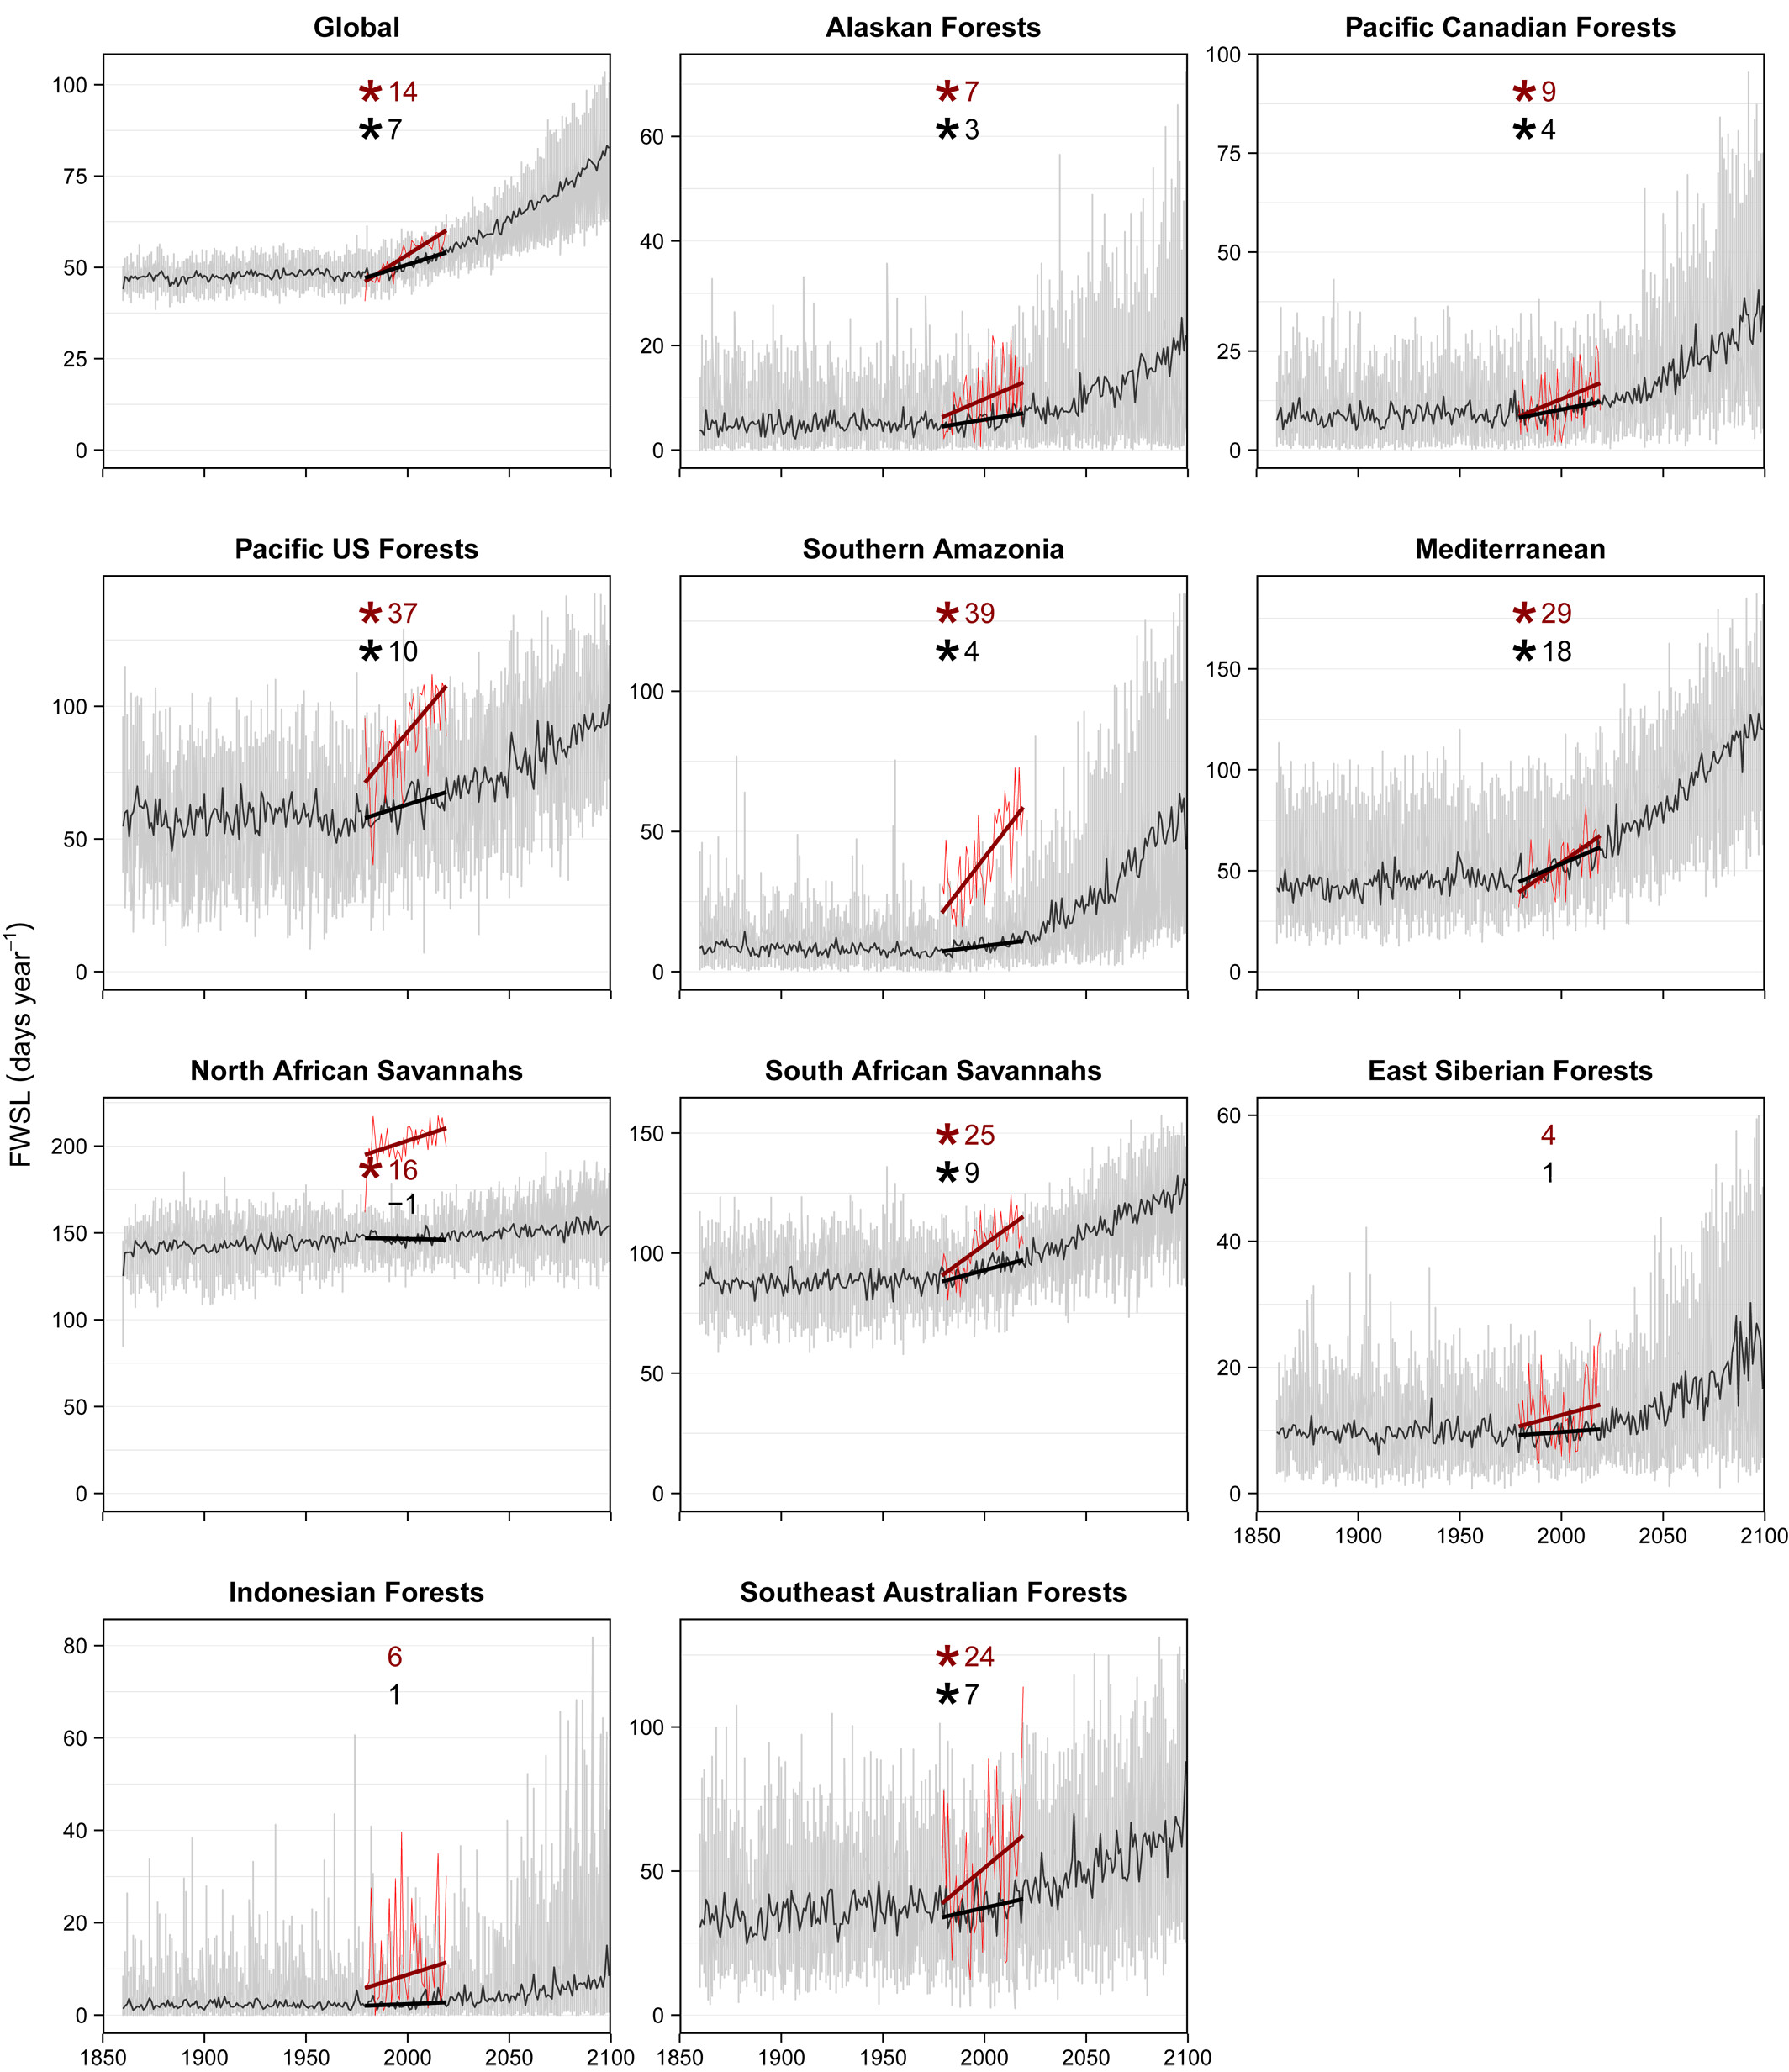
\includegraphics[width=0.95\linewidth]{images/FWSL_region_comparation.png}
%     \caption{\footnotesize{Time series of global and regional estimates of mean fire weather season length (FWSL) from measurements analyzed by ERA5 (thin red lines; Hersbach et al.,[2020]; Vitolo et al., [2020] and CMIP5 models running RCP8.5 (gray lines; Abatzoglou et al., [2019]. Thin black lines mark the multi-model mean estimate from the CMIP5 models. Linear trends in the period 1979–2019 are shown for the ERA5 (thick red lines) and CMIP5 (thick black lines), with corresponding numbers marking the change in annual FWSL during the period (the slope integrated over the period 1979–2019) and corresponding asterisks denoting significant changes at the 95\% confidence interval. Differences between modeled and observed FWSL can be explained by differences in the resolution of the models (2.5°) versus the observations (0.25°), since FWSL is partly determined by the maximum value FWI and this is reduced through spatial averaging.\protect\footnotemark}}
%     \label{fig:fire_season_FWSL_1979_2019}
% \end{figure}
% \footnotetext{\label{fn:jones2022}\footnotesize{Reproduced from Jones \emph{et al.} (2022), \cite{effisPRTstats}. Licensed under \href{https://creativecommons.org/licenses/by/4.0/}{CC BY 4.0}.}}

% \begin{figure}[H]
%     \centering
%     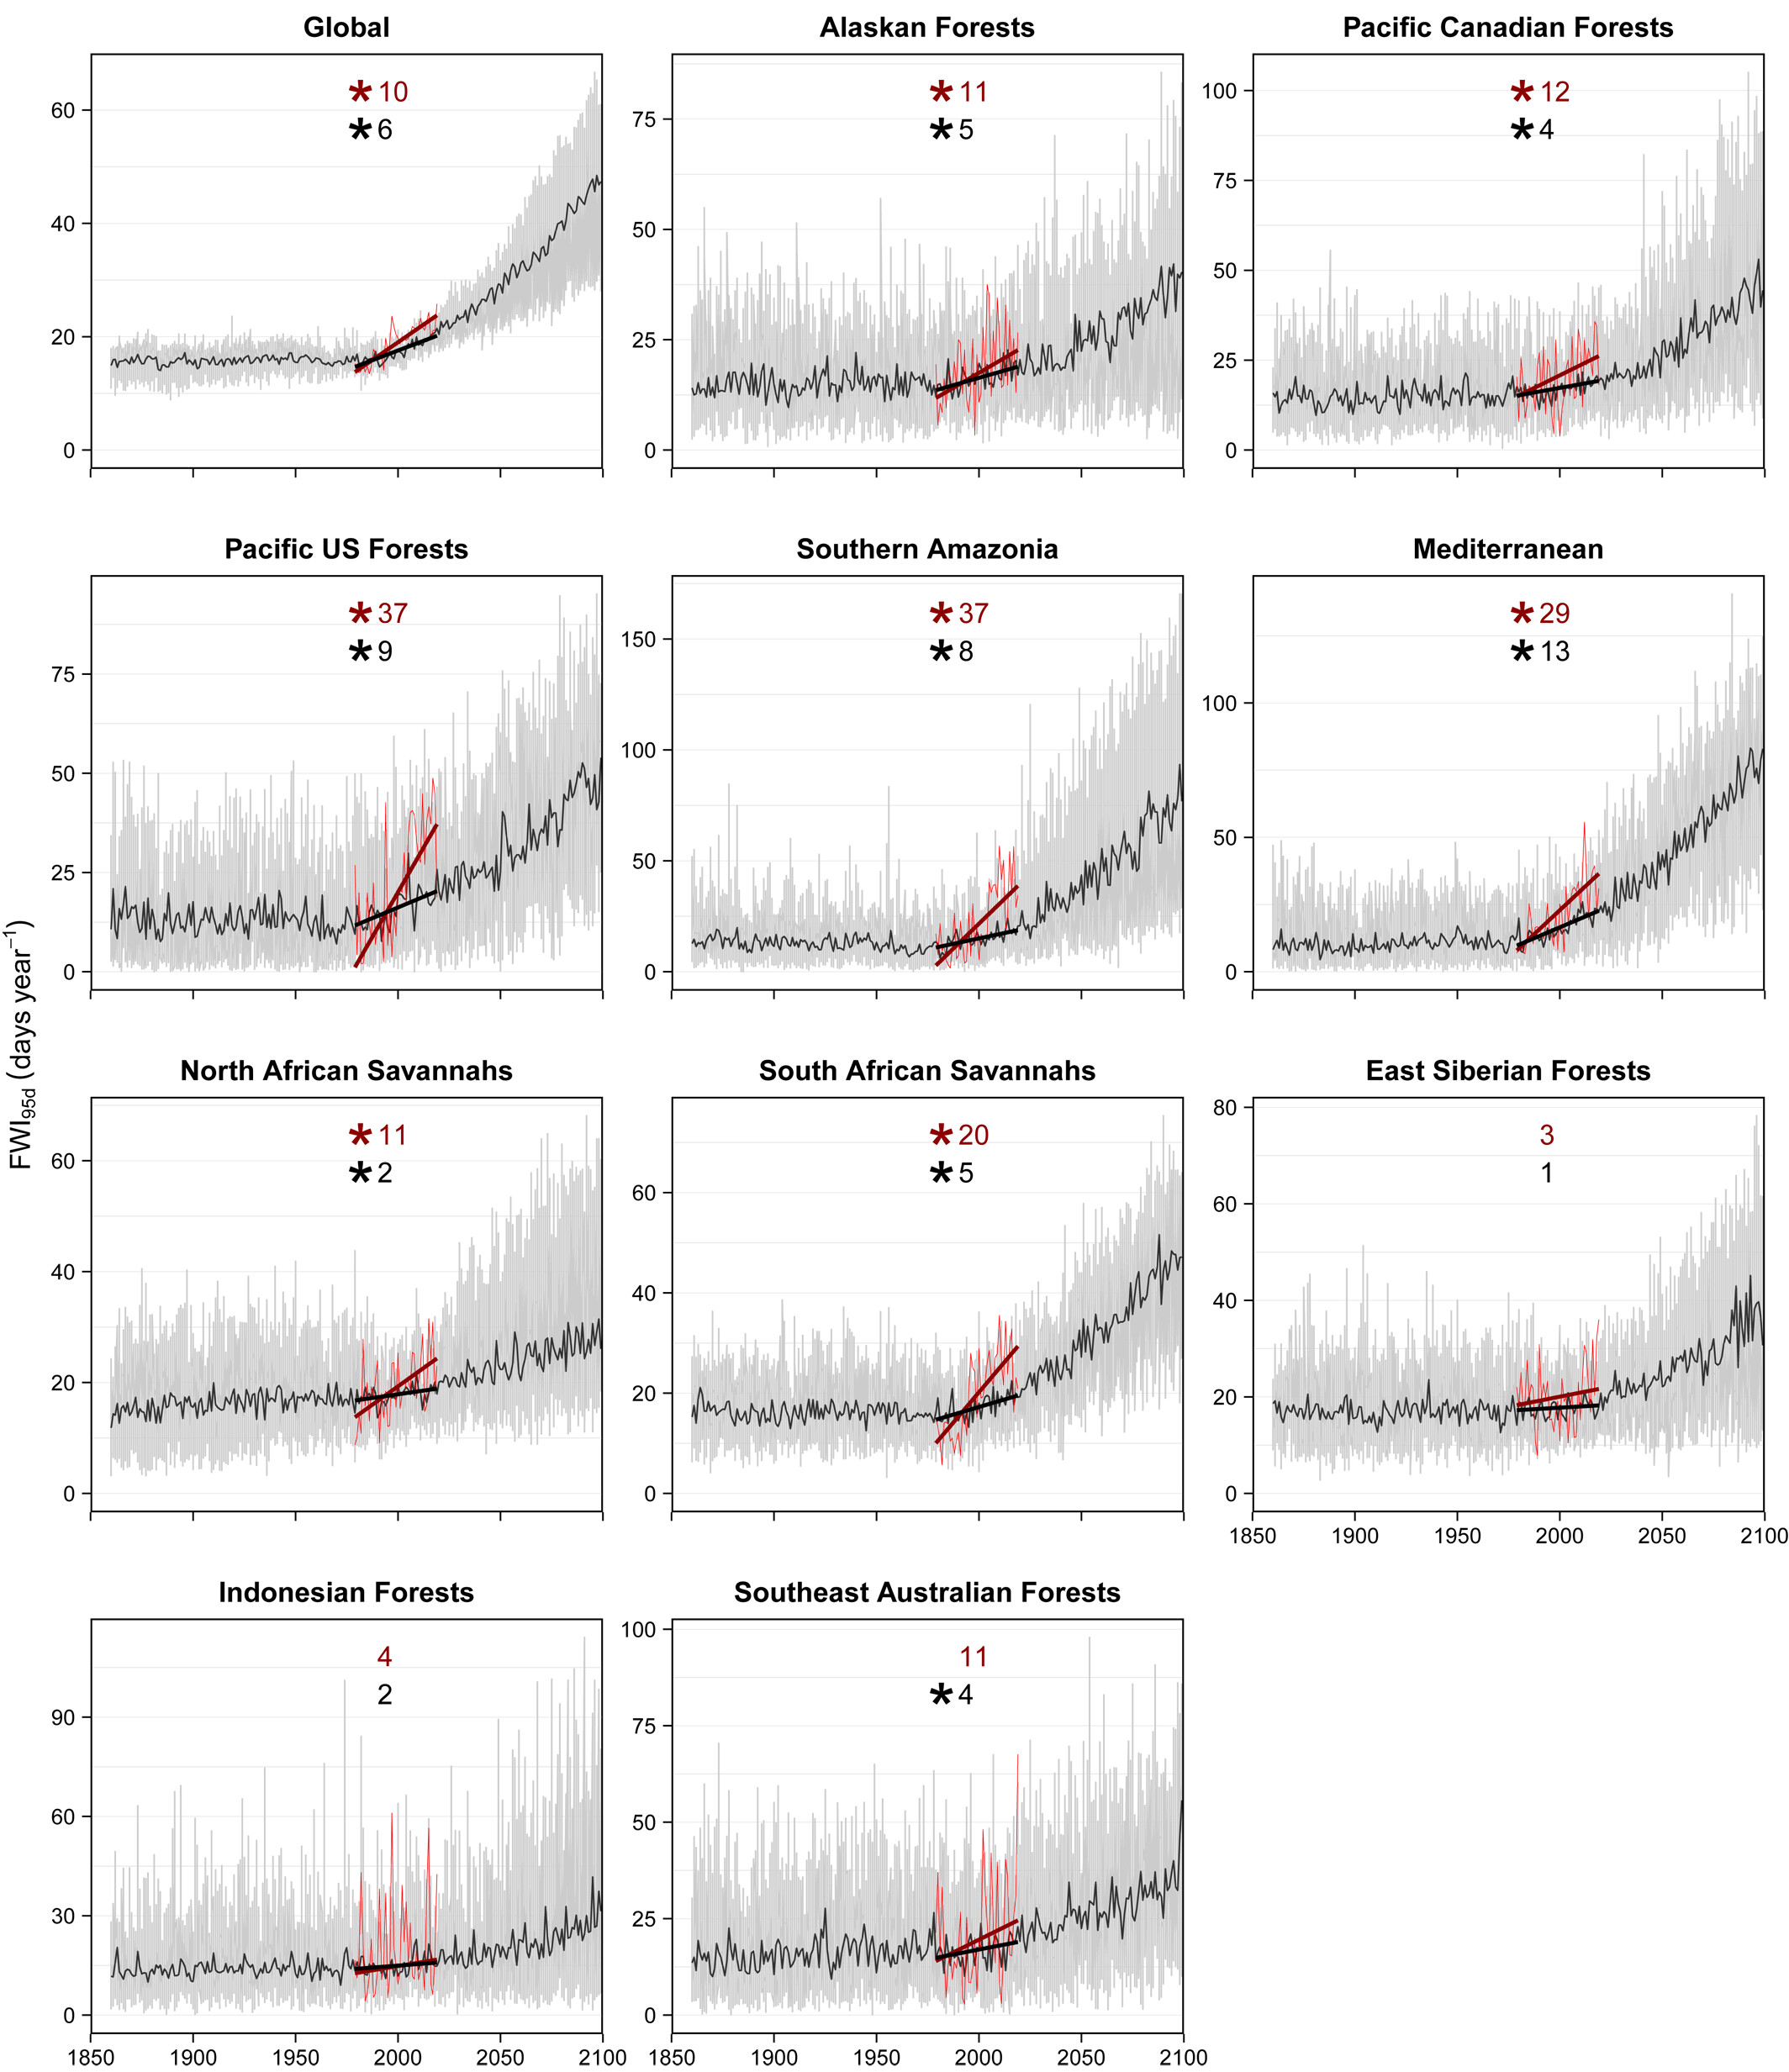
\includegraphics[width=1\linewidth]{images/region_comparation_fire_index.png}
%     \caption{Time series of global and regional estimates of mean FWI95d from ERA5 (thin red lines; Hersbach et al., 2020; Vitolo et al., 2020) and CMIP5 models running RCP8.5 (gray lines; Abatzoglou et al., 2019). Thin black lines mark the multi-model mean estimate from the CMIP5 models. Linear trends in the period 1979–2019 are shown for the ERA5 (thick red lines) and CMIP5 (thick black lines), with corresponding numbers marking the change in annual FWSL during the period (the slope integrated over the period 1979–2019) and corresponding asterisks denoting significant changes at the 95\% confidence interval.\textsuperscript{\ref{fn:jones2022}}}
%     \label{fig:fire_extreme_days_freq_FWSI95d_1979_2019}
% \end{figure}

% \begin{figure}[H]
%     \centering
%     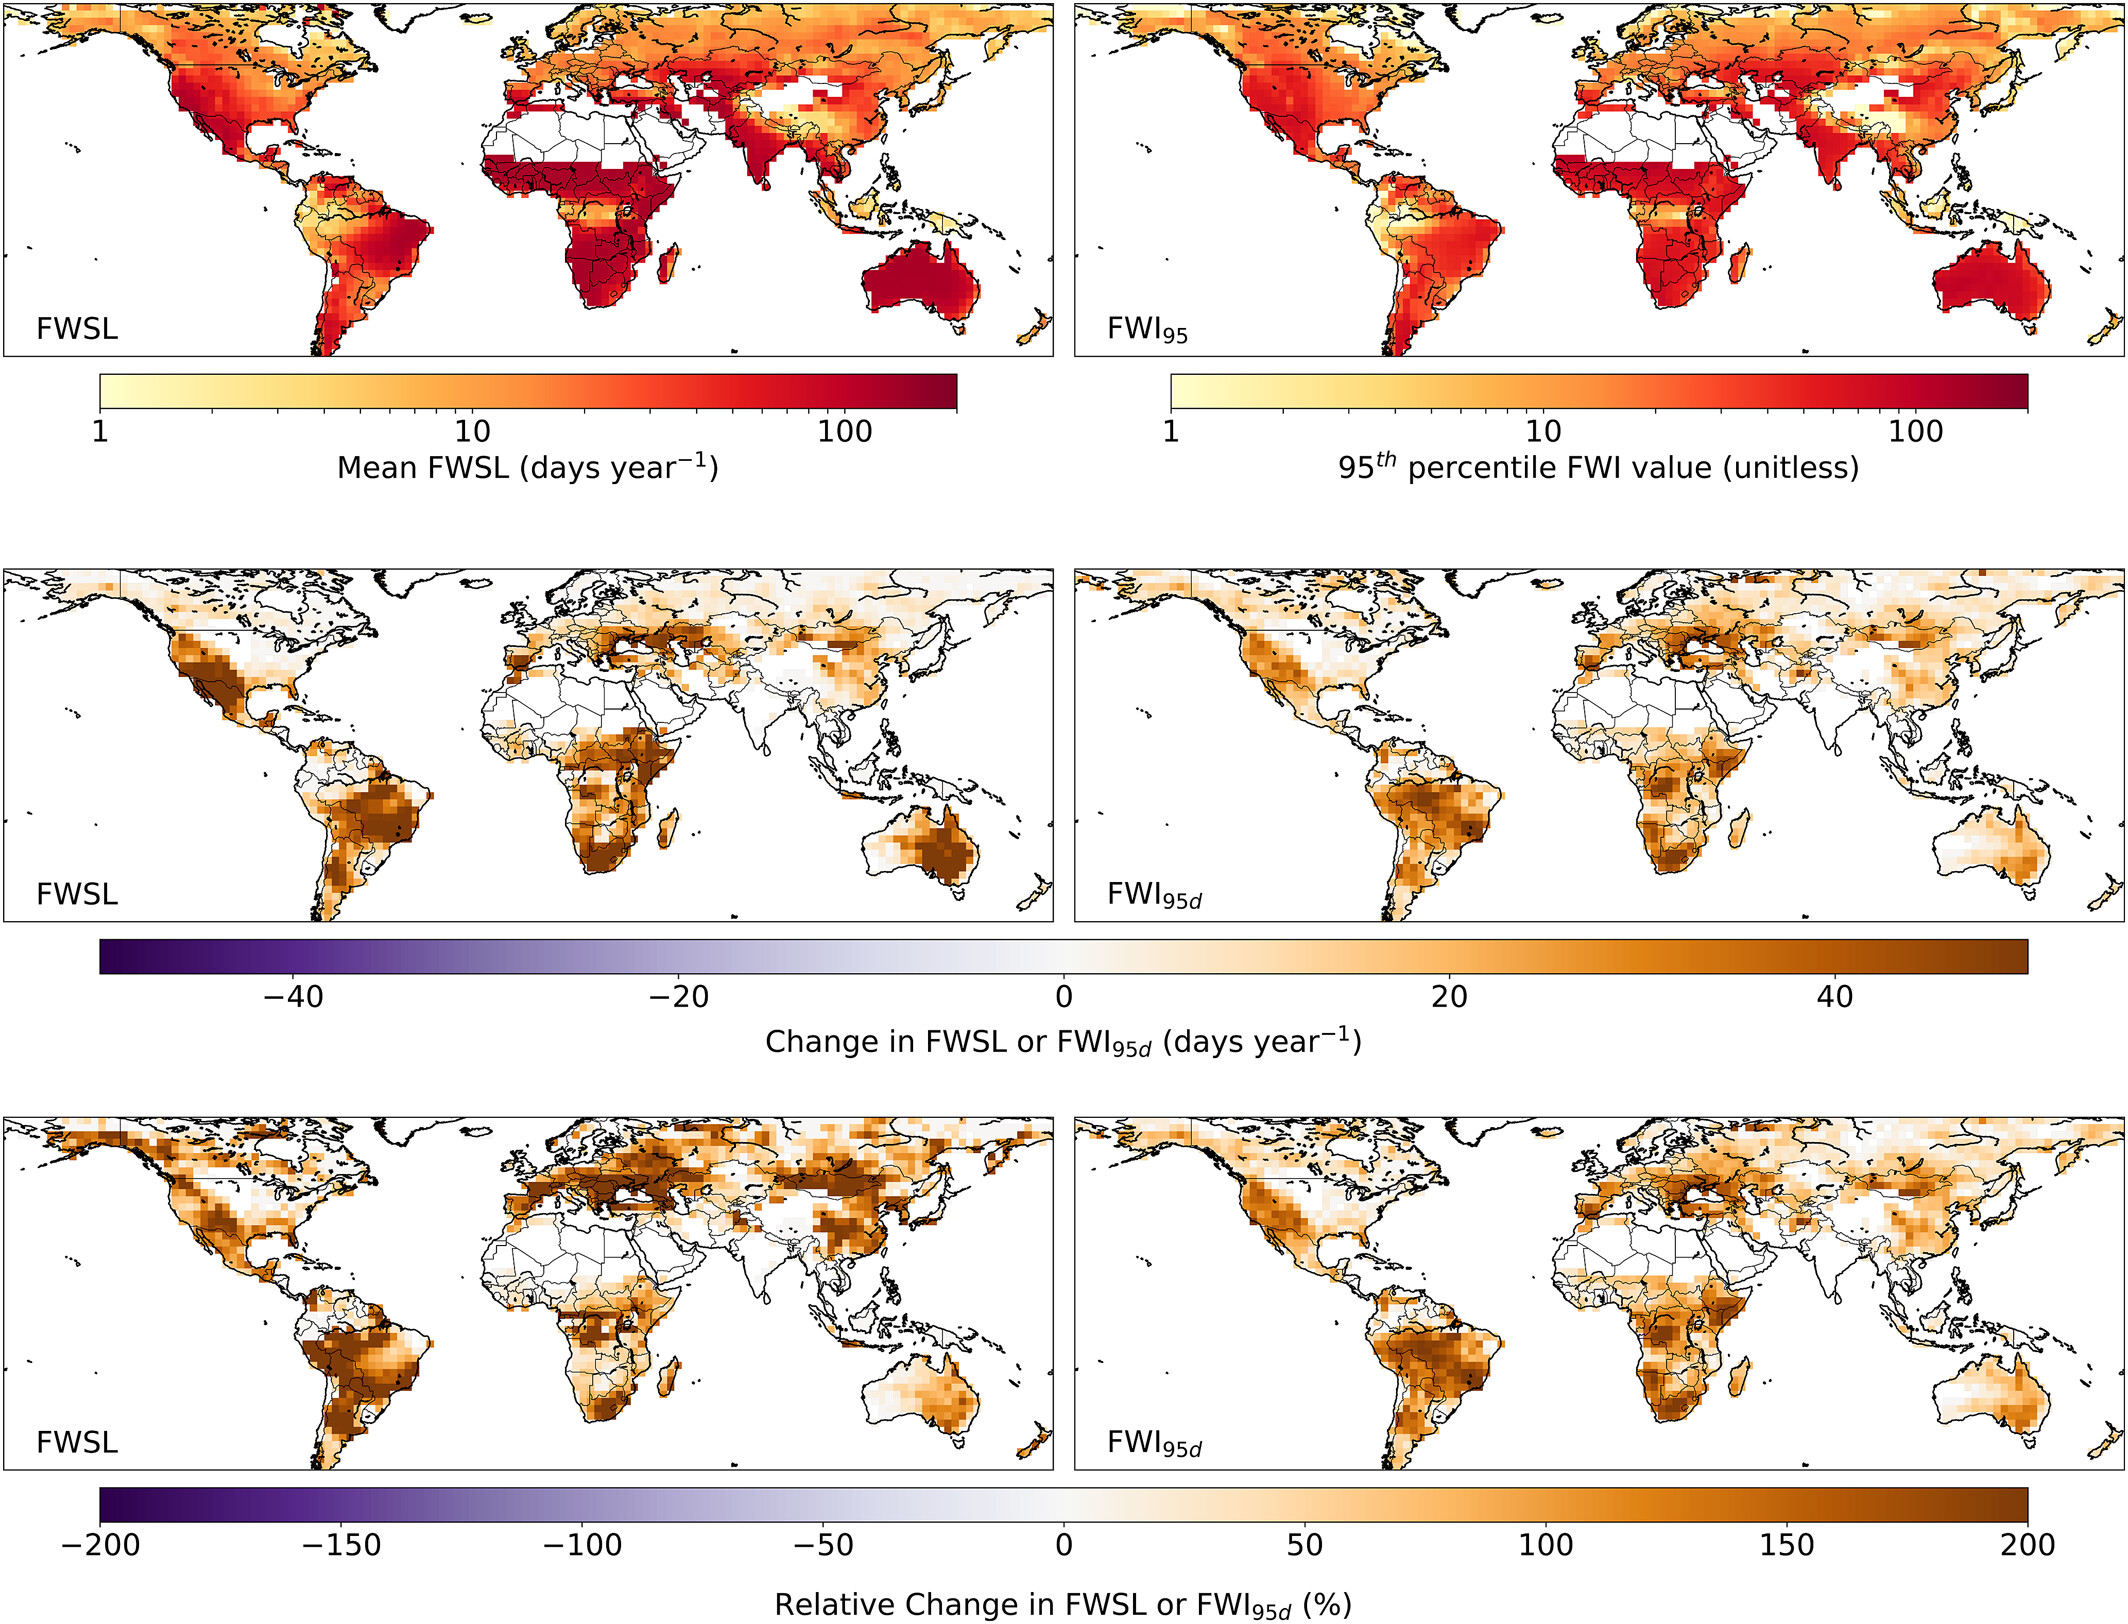
\includegraphics[width=1\linewidth]{images/FWSL_FWI95d_1979_2019_mean_absolute_relative.png}
%     \caption{Global patterns and trends in fire weather during 1979–2019 based on ERA5 reanalysis data (Hersbach et al., [2020]; Vitolo et al., [2020]. (Left panels) include (top) mean, (middle) absolute change and (bottom) relative change in annual fire weather season length (FSWL) during 1979–2019. (Right panels) include (top) the 95th percentile daily value of fire weather index (FWI) threshold value during 1979–2019, (middle) the absolute change in annual days with FWI values exceeding the 95th percentile and (bottom) the relative change. Absolute change (days year−1) is calculated as the trend (days year−2) multiplied by the length of the time series (41 years). The relative change is the absolute change divided by the mean.\textsuperscript{\ref{fn:jones2022}}}
%     \label{fig:map_FWSL_FWI95d_change_relative_1979_2019}
% \end{figure}

% \begin{figure}[H]
%     \centering
%     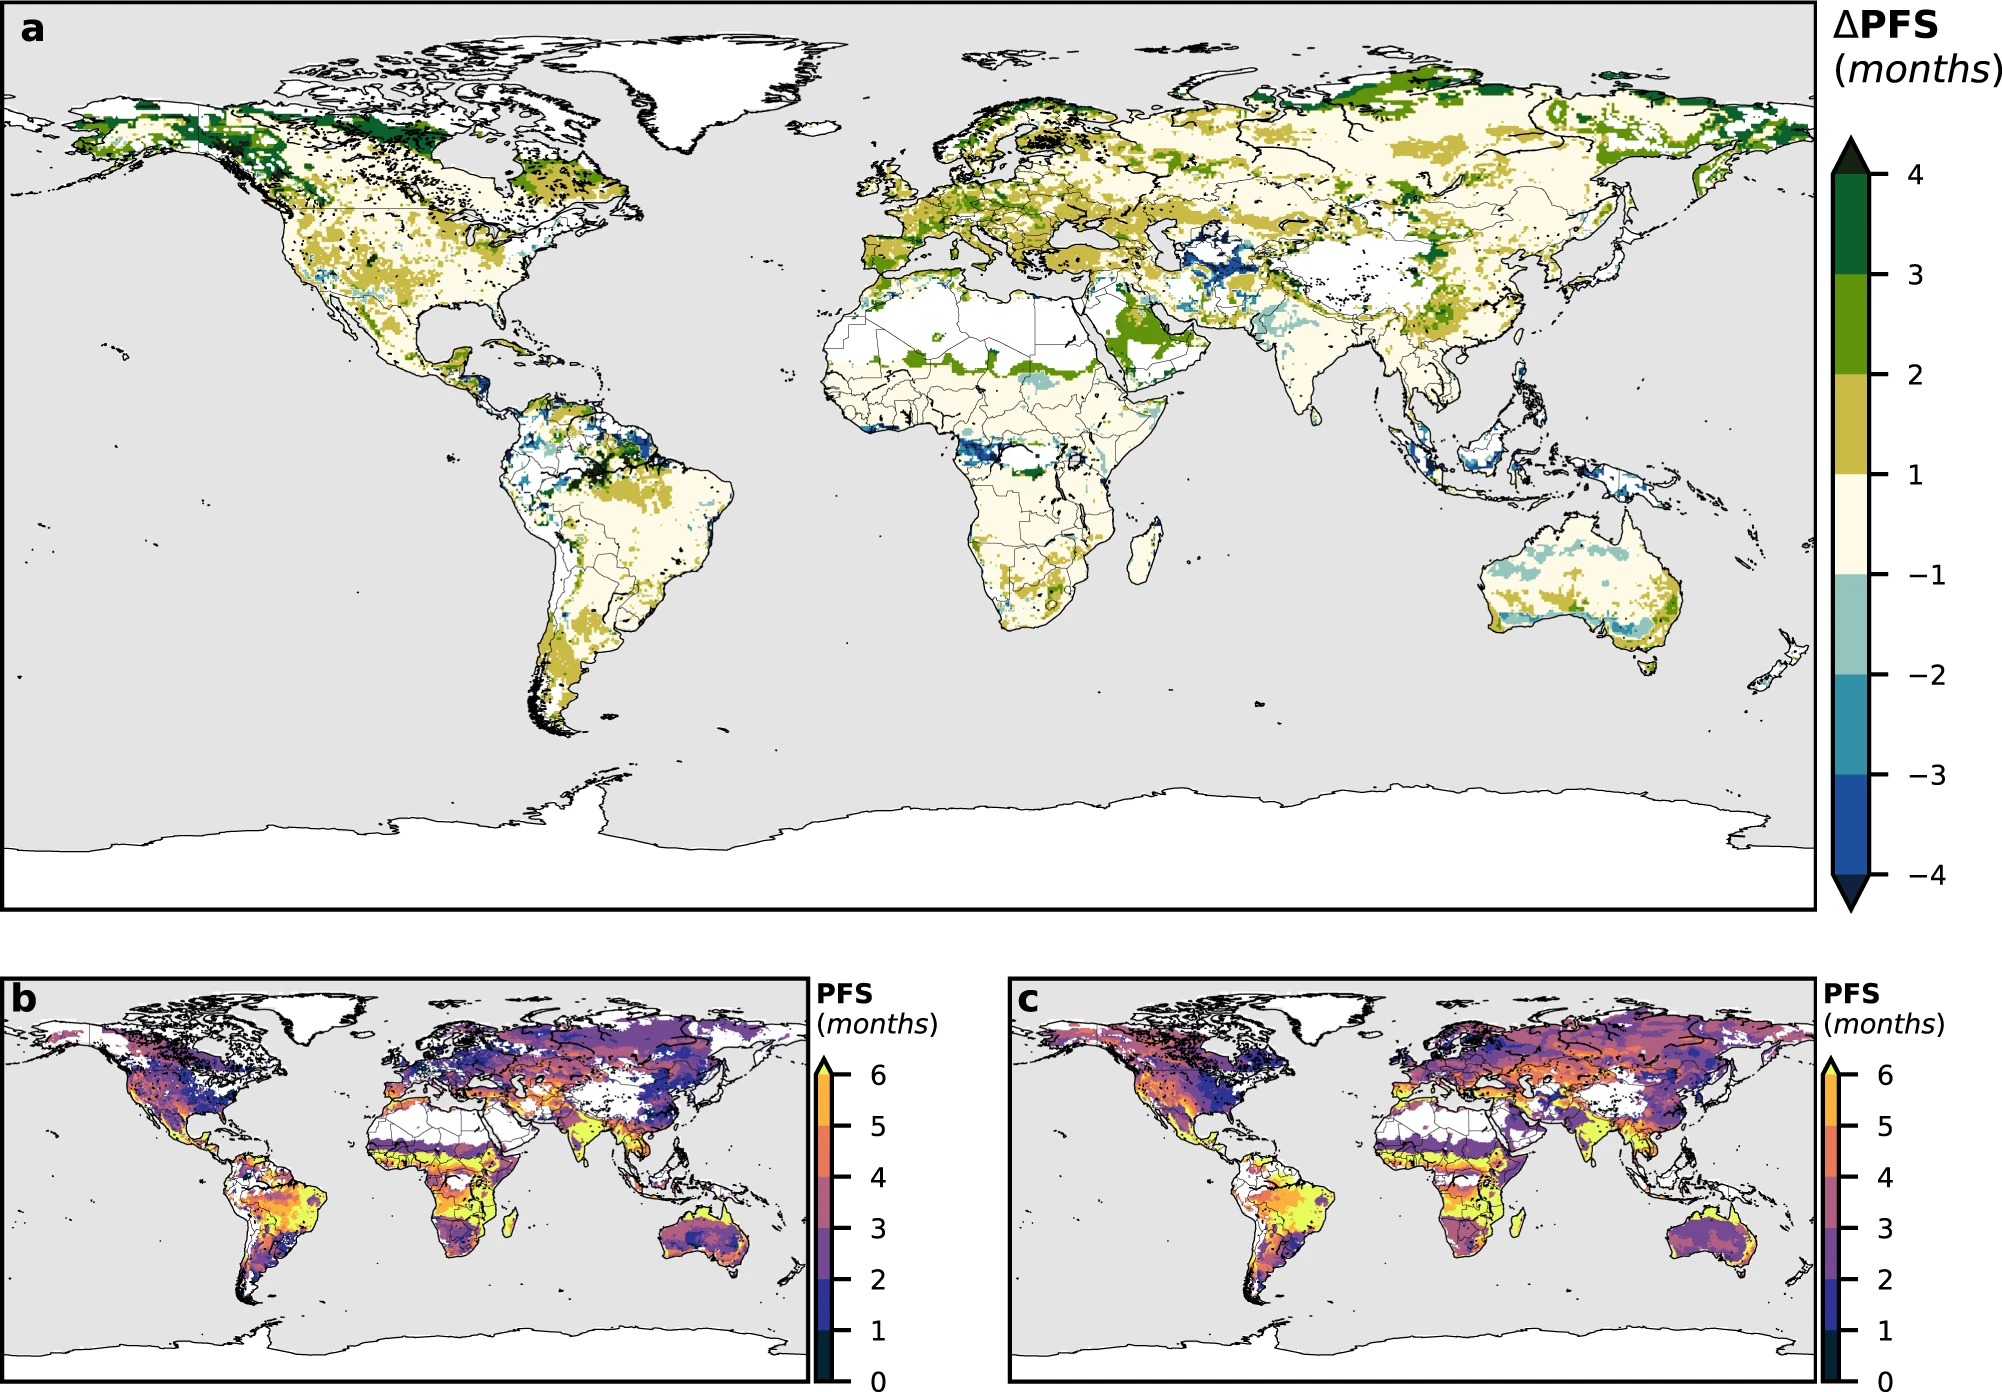
\includegraphics[width=1\linewidth]{images/fire_season_global_change_future_present.png}
%     \caption{(TODO:Add this analysis) a Future minus present potential fire season length (PFSL) difference in months (ΔPFSL). b Present potential fire season. c Future potential fire season.https://www.nature.com/articles/s41467-022-28835-2/figures/3}
%     \label{fig:fire_season_global_change_future_present}
% \end{figure}

% \begin{figure}[H]
%     \centering
%     \includegraphics[width=1\linewidth]{images/map_prediction_dT4_FWSL_FWI.png}
%     \caption{Enter Caption}
%     \label{fig:map_prediction_dT4_FWSL_FWI}
% \end{figure}

% \paragraph{Conclusion.}
% Taken together, the Great Acceleration framing and multi-model fire-weather diagnostics indicate that anthropogenic forcing has already emerged in regional fire climates and is lengthening the window of high-risk conditions while increasing the frequency of extreme fire-weather days \cite{steffen2015trajectory,abatzoglou_global_2019,jones_global_2022}. These signals are especially pronounced in Mediterranean-type climates and across key tropical biomes, where land-use legacies and expanding wildland–urban interfaces amplify ignition pressure and losses. In practical terms, if biomass as fuel is available, the climate crisis is converting more days into days when fires start faster, spread farther, and are harder to control. This establishes the operational need that motivates the present work: a high-temporal, sufficiently resolved, low-latency orbital sensing capability that can shorten detection and modeling feedback loops. The next subsections therefore narrow from the global picture to Portugal—situated within a Mediterranean hotspot—to articulate why current, low-revisit imagery is mismatched to the new hazard regime and how a dedicated constellation can enable earlier detection, better spread forecasts, and more effective firefighting.




% \subsection{Burned Area Trends}

% \subsubsection{Decreasing in Global Burned Area}

% Although the past, present, and future Fire Weather Index (FWI) predictions are important for indicating fire danger in a specific spacetime region on Earth, the FWI alone does not measure fire activity or the actual damage caused to the environment. By managing the availability of flammable biomass, a region with high FWI danger may have a null Burned Area (BA) without destruction. Therefore, the \textit{metric that truly measures fire damage is the BA}.

% Before the advent of Earth observation satellites, historical series measurements of BA on a global scale were neither accurate nor readily accessible. The 1960s and 1970s marked the beginning of spaceborne BA measurements. Consequently, to estimate BA future or past trends, simulation models were developed based on the BA satellite-observation database. 

% A modern example of a BA model is the Fire Model Intercomparison Project (FireMIP), which is a combination of X models.  On Fig \ref{fig:regional_series_fireMip} we can see FireMIP BA analysis between 1900-2020. On this plot, the Global BA matches closely the FireMip\textbf{ median BA prediction of ~\(4.3 \times 10^{6}\ \mathrm{km^{2}\,yr^{-1}}\)  on the period between 2000 an 2015}. During this temporal interval, it is possible to observe a \textbf{global decreasing trend in BA }not only in the model prediction, but also in the observed satellite data of MODIS (red line). 
% A detailed BA trend of the same period was also conducted by Giglio et al., and it is shown in Fig  \ref{fig:BA_global_trend_regions}. This plot displays a \textbf{global decreasing trend in BA aproximately \(-1.1 \times 10^{6}\ \mathrm{km^{2}\,}\) per year.} \textbf{(Giglio et al. 2018 - MISSING CITATION)}. Besides BA model trends, Andela et al. (2017) used satellite data to create a visualization of the observed BA from satellites, which is shown in Fig. \ref{fig:map_BA_global_decrease_1998_2015}. This study confirms the decreasing global trend, with a measured \textbf{decline in BA of -24.3 ± 8.8\% between 1998 and 2015}.

% Considering the rise in global temperatures, the increasing impacts of the climate crisis, and the longer, more intense fire seasons, this reduction in the global BA trend is unexpected. This paradox is interpreted by Jones et al. (2022) as a "global BA decline since 2001 driven primarily by large reductions of BA in African savannas, where land-use change (cropland expansion, livestock grazing, fragmentation, and enhanced suppression), and regionally reduced vegetation productivity under drier hydrological conditions that limited fuel and fire spread, decoupling burned area trends from the concurrent increases in fire weather index.”

% \begin{figure}
%     \centering
%     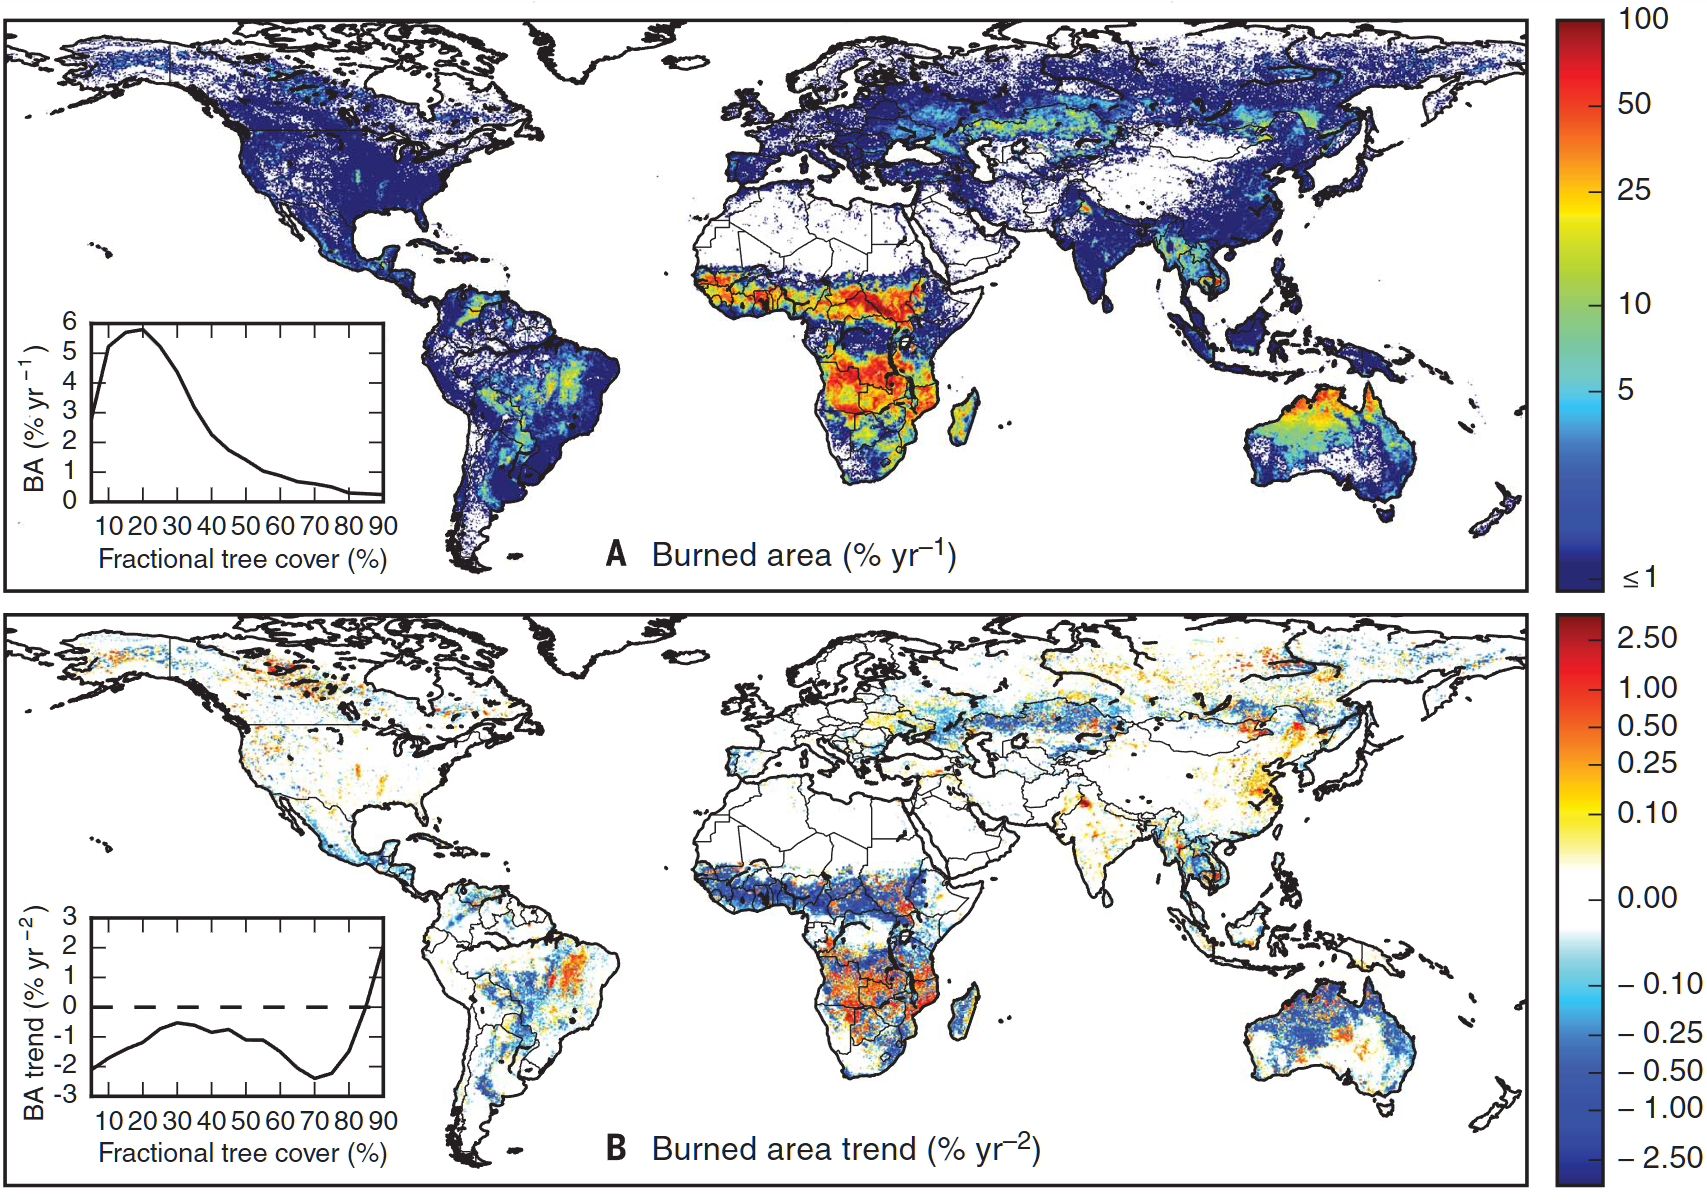
\includegraphics[width=1\linewidth]{images/map_BA_global_decrease_1998_2015.png}
%     \caption{\small{Satellite observations show a declining trend in fire activity across the world’s tropical and temperate grassland ecosystems and land-use
% frontiers in the Americas and Southeast Asia. (A) mean annual burned area and (B) trends in burned area (GFED4s, 1998 through 2015). Line plots (inset)
% indicate global burned area and trend distributions by fractional tree cover}}
%     \label{fig:map_BA_global_decrease_1998_2015}
% \end{figure}



% Explan correlations

% \begin{figure}[H]
%     \centering
%     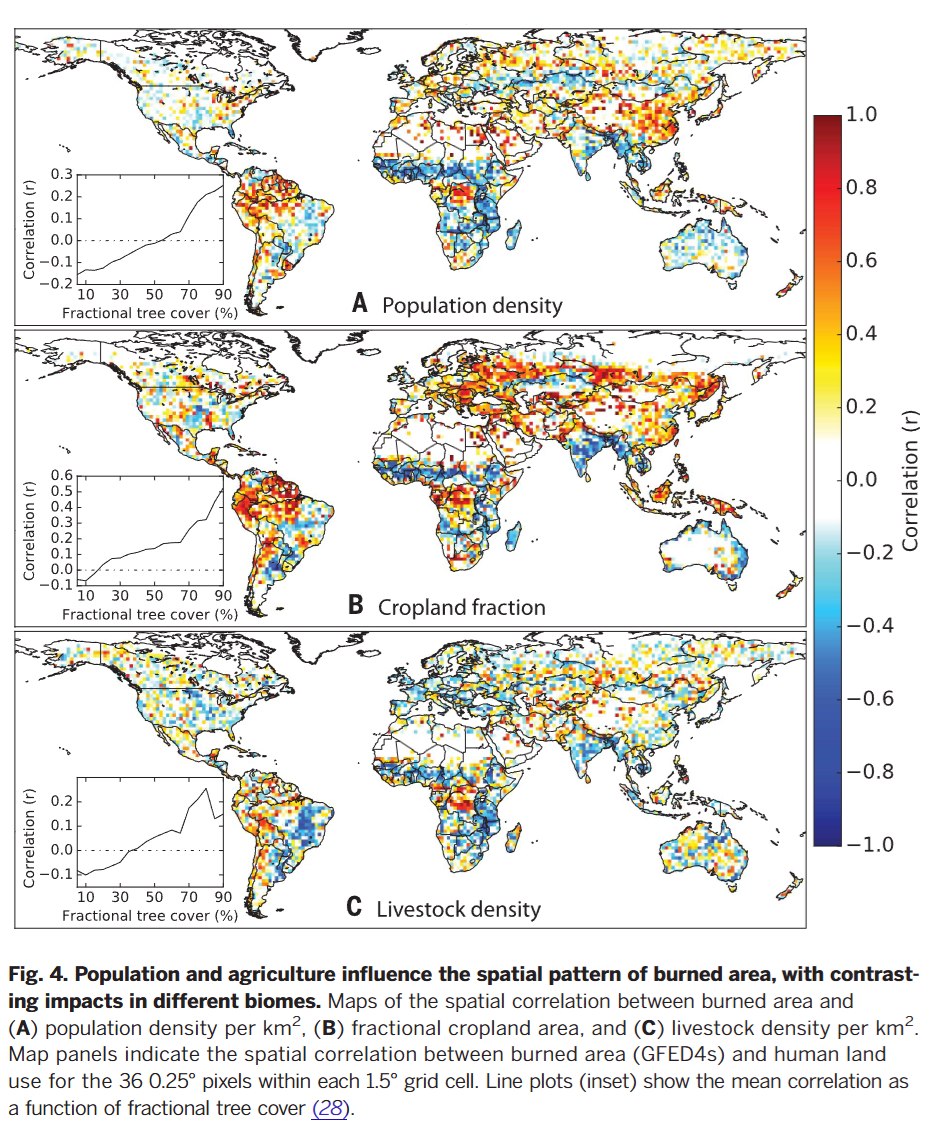
\includegraphics[width=1\linewidth]{images/map_BA_correlation_population_cropland_livestock.png}
%     \caption{Enter Caption}
%     \label{fig:map_BA_correlation_population_trends}
% \end{figure}
% \subsubsection{Increase in Regional Burned Area}

% Although global BA has declined since the 2000s, multiple studies report regional increases in burned areas in different types of ecosystems. Fig \ref{fig:map_BA_global_decrease_1998_2015} -B demonstrates the regions where the burned area trend is still increasing. The design of the satellite constellation shall have as secondary Regions of Interest (ROIs) the ecoregions with frequent incident wildfires. This subsection's goal is to indicate what these potential ROIs are, give details of recent BA activity, and provide some correlations that is connected with the fire activity. 

% Andela et al. (2017) found that, despite a ~24\% global BA decline (1998–2015), areas of significant BA increase were widespread across Eurasia’s closed-canopy forests (boreal and temperate), even as savanna/grassland BA—the dominant global contributor—contracted with cropland expansion, grazing, and fuel fragmentation. 

% Jones et al. (2001–2019) report rising BA in several forest ecoregions—e.g., Pacific U.S. forests (~+49\%), Pacific Canada (~+63\%), and East Siberian boreal forests (~+93\%)—noting that short records and high interannual variability make some trends statistically non-significant at the grid/ecoregion scale. 

% Extending the satellite record, GFED5 (1997–2020) shows positive BA trends across many high-northern boreal ecosystems (e.g., Siberia and the Russian Far East), consistent with warming-driven fuel aridity and longer fire seasons in closed-canopy needleleaf forests. 

% Complementary evidence based on forest loss attributed to fire (2001–2019) indicates a global increase in fire-related forest loss, with strongest contributions from boreal Eurasia, and additional signals in humid/tropical and temperate forests, underscoring that forest biomes (rather than savannas) are driving the emergent increases. 

% Looking over longer baselines, circumboreal syntheses show ~50\% higher BA from the 1980s to the 2010s, with significant increases over substantial closed-canopy areas, reconciling the global decline (savanna-driven) with rising forest fire activity at higher latitudes.

% \begin{figure}[H]
%     \centering
%     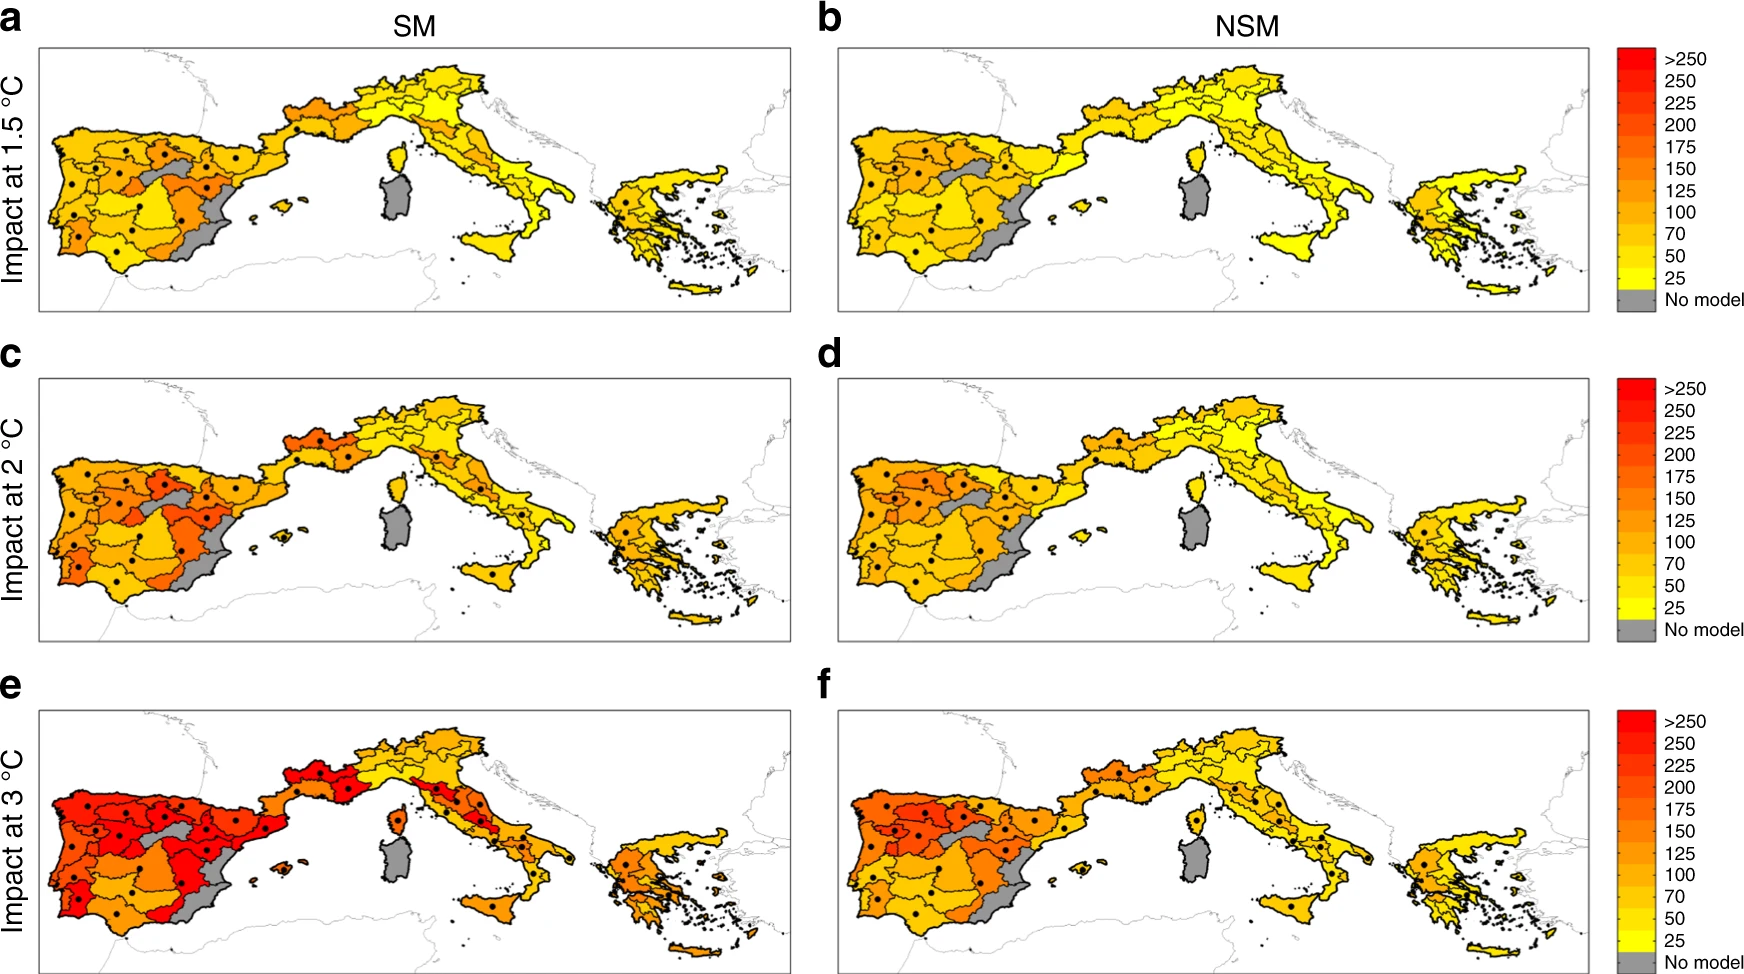
\includegraphics[width=1\linewidth]{images/mediterranean_fire_increase.png}
%     \caption{Ensemble mean burned area changes. Burned area changes (\%) for a the +1.5°C case with the stationary model SM (i.e., using Eq. 3), (b) the +1.5°C case with non-stationary model NSM (i.e., NSM). using Eq. (4), (c) the +2°C case with SM, (d) the +2°C case with NSM, (e) the +3°C case with SM, and f the +3°C case with NSM. Dots indicate areas where at least 50\% of the simulations (1000 bootstrap replications × the ensemble of RCMs) show a statistically significant change and more than 66\% agree on the direction of the change. Coloured areas (without dots) indicate that changes are small compared to natural variations, and white regions (if any) indicate that no agreement between the simulations is found}
%     \label{fig:mediterranean_fire_area}
% \end{figure}


% \subsection{Burned Area Trends Vs Correlations}






% \subsubsection{Rise of Forest Burned Area}

% IPCC-assessed projections indicate Mediterranean burned area could increase by \(\sim\)40–54\% at 1.5\(^{\circ}\)C, 62–87\% at 2\(^{\circ}\)C, and 96–187\% at 3\(^{\circ}\)C, with compound hot–dry extremes and drought driving large-fire risk\cite{turco_exacerbated_2018}.\footnote{\textit{Side note—Mediterranean risk:} Tenfold increases in the probability of catastrophic fire years are possible in parts of southern Europe under moderate CMIP6 scenarios \cite{elgarroussi_europe_2024}, and repeated fires can shift Mediterranean forests toward shrublands; paleorecords show that crossing precipitation thresholds ($\approx$40–45\% below interglacial levels) triggered abrupt forest–to–steppe transitions in the past, underscoring limited resilience under sustained aridification \cite{koutsodendris_atmospheric_2023,baudena_increased_2020}. The Mediterranean warms \(\sim\)20\% faster than the global average and WUI now covers \(\sim\)7.4\% of Europe, heightening exposure; recent EFFIS/JRC reports confirm that 2023 was among the worst EU wildfire years on record, dominated by the Mediterranean.} 

% The study done by Abatzoglou et al.\cite{abatzoglou_global_2019} also indicates the affected area is projected to enlarge under continued warming. In places where vegetation and ignitions are available, this translates into rising fire potential and heightened management challenges, which call for orbital sensors to assist in wildfire management \cite{abatzoglou_global_2019}.



% \section{Event cycles of wildfire --- Global \& Portuguese
% case}\label{22-event-cycles-of-wildfire-----global--portuguese-case}

% Show \textbf{global/biome monthly seasonality} (heatmaps or histograms)
% to characterize \emph{when} fires occur by regime; produce a neutral
% \textbf{seasonality atlas} of peak months across major pyro-regions.
% \textbf{Output:} a global reference calendar used later to benchmark
% Portugal and to define optional \textbf{secondary performance
% capability} tests for a Portugal-centric constellation in other regions'
% peak seasons.

% \begin{figure}
%     \centering
%     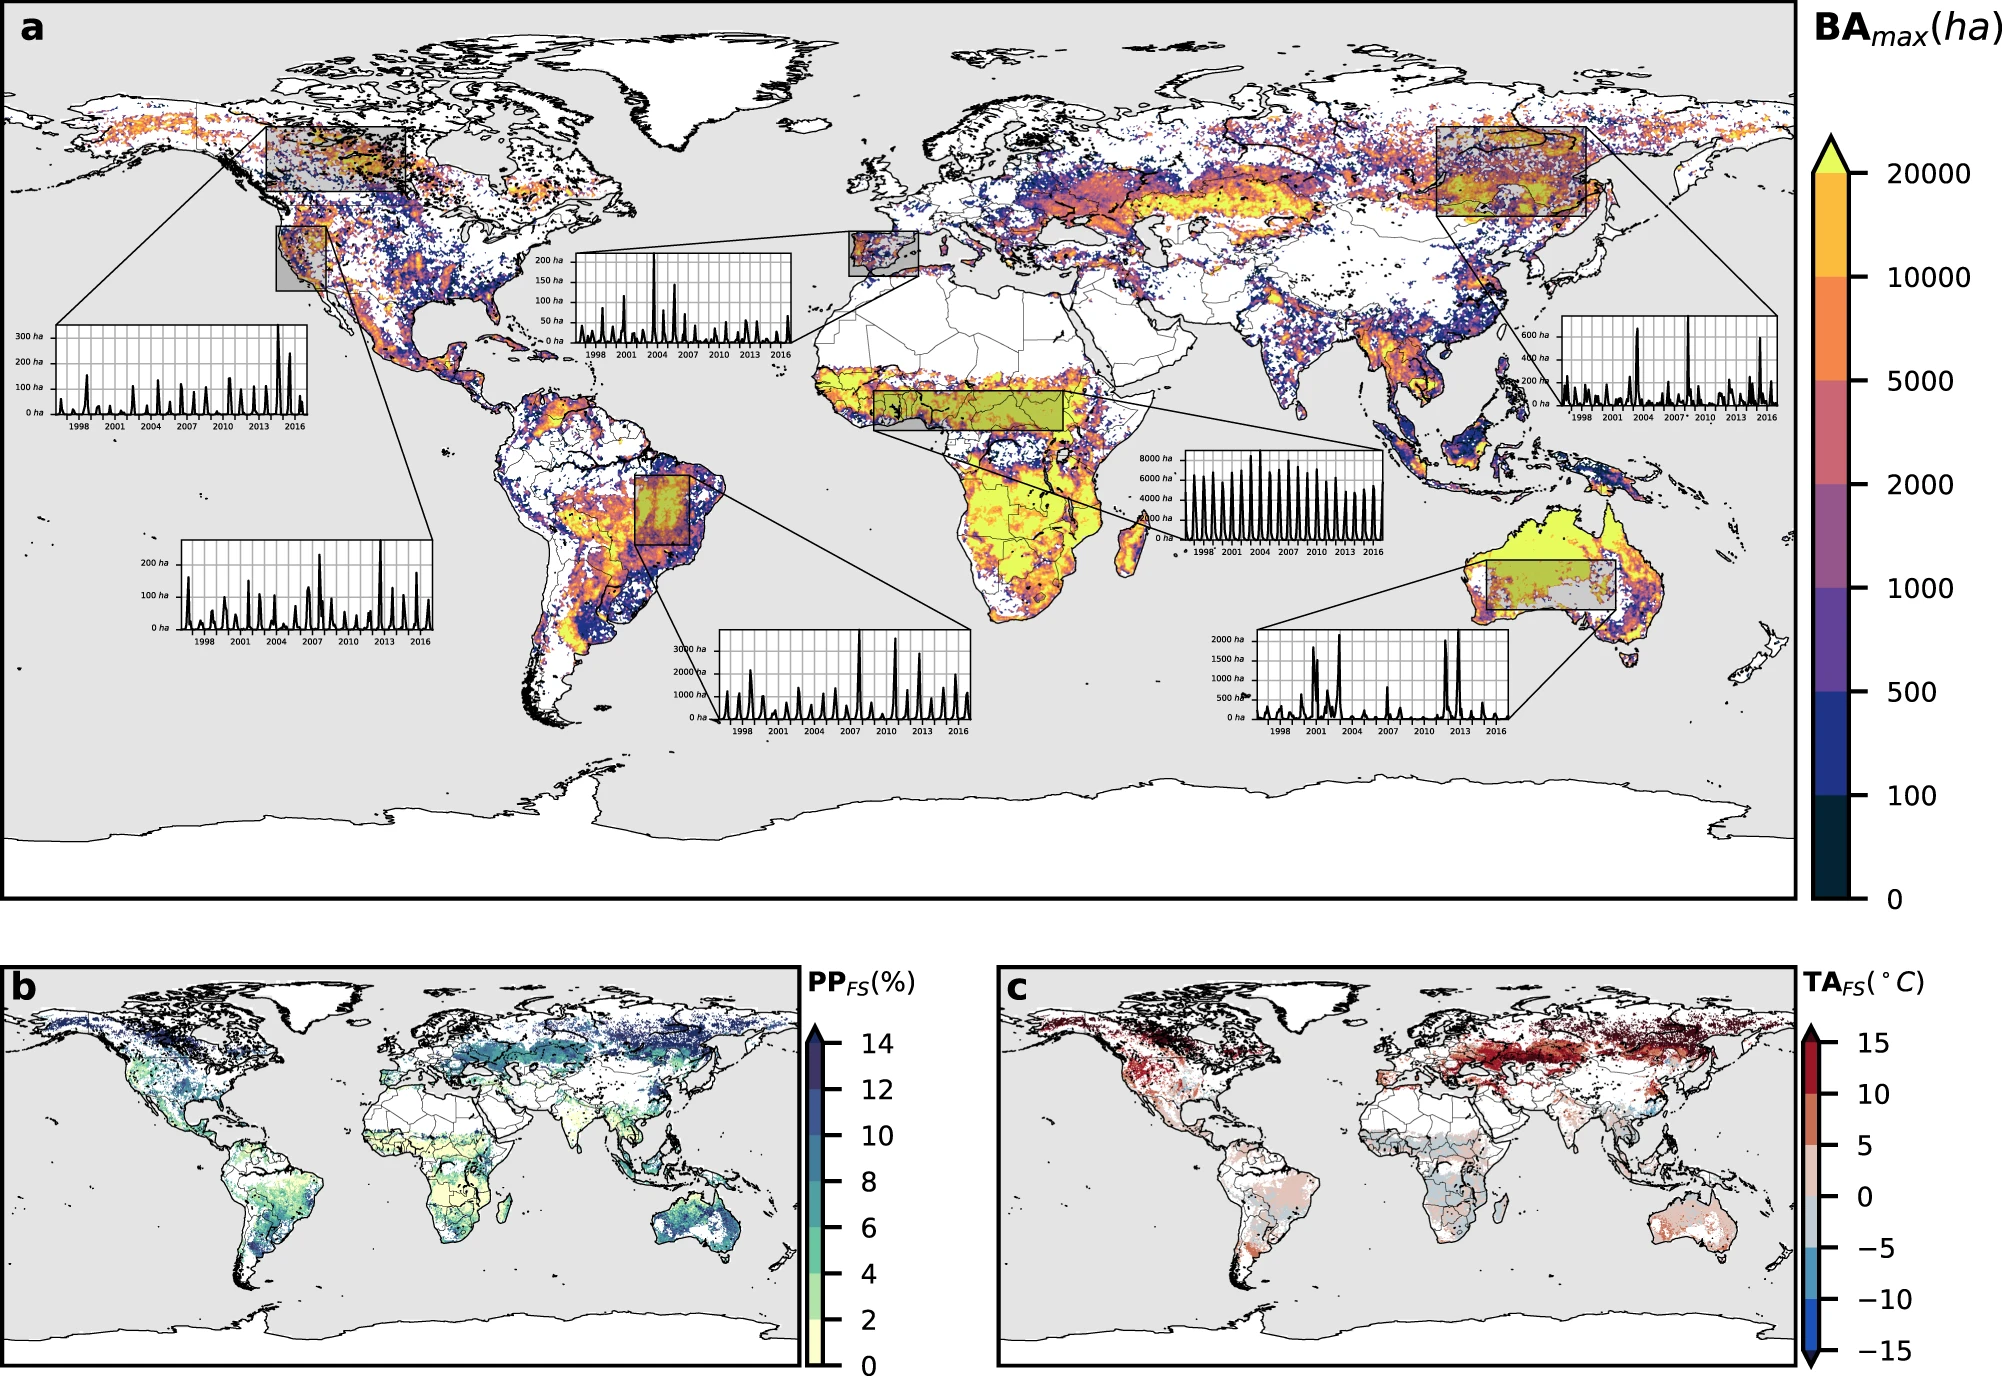
\includegraphics[width=1\linewidth]{images/BA_global_decade_fire_seasons.png}
%     \caption{1996–2016 maximum annual burned area (BAmax) and monthly burned area time series for selected regions. b Average monthly precipitation percentage from the annual total for the fire season (PPFS). c Average monthly temperature anomaly from the annual mean for the fire season (TAFS) https://www.nature.com/articles/s41467-022-28835-2/figures/1.}
%     \label{fig:BA_global_decade_fire_seasons}
% \end{figure}

%--------------------

This chapter establishes the observational study domains that define where and when the satellite constellation must observe. It begins by formalising the mission environment as a four-dimensional manifold connecting the inertial and Earth-fixed reference frames, and then defines two complementary study domains: the \textit{Core Study Domain} ($\mathcal{D}_{core}$), spatially bounded by mainland Portugal and temporally aligned with its fire season, and the \textit{Global Study Domain} ($\mathcal{D}_{global}$), which extends the analysis to all fire-prone regions classified by climate regime and fire frequency. The chapter concludes by introducing the FIRMS geostationary active-fire dataset as the high-cadence empirical reference for constellation verification, and by consolidating the derived requirements (R9--R25) that constrain the mission simulation.

\section{Observational Study Domains} \label{sec:obs_domains}

Depending on the dynamic interactions among biomass, climate, and human activity, each region of interest observed by the satellite could exhibit a characterizable fire intensity over a temporal pattern; in other words, each region of interest could have a specific fire season. With this in mind, the satellite constellation mission modeled in this work shall have as a requirement an observational temporal window synchronized with these fire season periods. Therefore, the spacecraft architecture shall be analyzed against\textit{ Fire-Prone Regions (FPR)}, or piroregions, here defined as the \textit{Core Study Domain ($\mathcal{D}_{core}$)} and the \textit{Generalized Study Domain ($\mathcal{D}_{general}$)}. Both of these objects are composed of subsets of \textit{Regions of Interest (ROI)} which are defined in a spatial $\mathcal{R}$ and temporal $\mathcal{T}$ coordinate domains. Therefore, each ROI can contain flammable biomass that may exhibit distinct fire dynamics over time, leading to a temporal spread of \textit{Fire Activity (FA)} in these domains. 

\subsubsection{Formal Definition of Study Domains}\label{sec:formal_def_domains}

To ensure the satellite constellation meets precise operational requirements, we define the mission environment as a four-dimensional manifold $\mathcal{M}$ (Space-Time). Since the satellite orbit is governed by orbital mechanics while the observation targets are subject to planetary dynamic motion, we must rigorously define the relationship between the inertial and rotating frames.

We establish the base reference frame of $\mathcal{M}$ as the \textbf{Earth Mean Equator and Equinox of J2000 (EME2000)}, hereafter denoted as the Inertial Frame $\mathcal{F}_{J2000}$ (corresponding to the IJK system in Fig. \ref{fig:vallado_ijk_frame}). However, the regions of interest for the constellation are fixed to the rotating Earth. Therefore, we define the boundaries of the study domains relative to the \textbf{World Geodesic System 84 (WGS84)}, which has an Earth-Centered Earth-Fixed (ECEF) frame, hereafter denoted as the Earth Frame $\mathcal{F}_{\oplus}$, \inlineReq{R9}.
\begin{figure}[H]
    \centering
    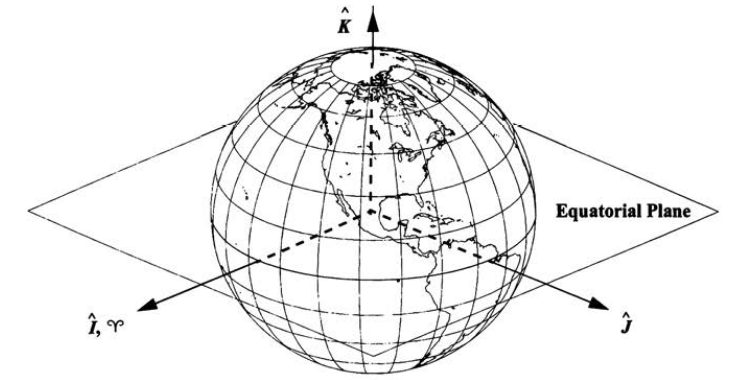
\includegraphics[width=0.65\linewidth]{images/Geocentric_Equatorial_System_(IJK)_F_earth.png}
    \caption{\footnotesize{The Geocentric Equatorial Coordinate System (IJK) as defined by Vallado \cite{mcclain2001fundamentals}. The frame is defined by Earth's origin, the equatorial plane, and the vector $\hat{I}$ pointing toward the Vernal Equinox ($\Upsilon$). In this thesis, the IJF frame system represents the Inertial Frame $\mathcal{F}_{J2000}$ used for orbit propagation. It is distinct from the rotating Earth Frame $\mathcal{F}_{\oplus}$ (ECEF), which holds the study Domain $\mathcal{D}$ that rotates with the Earth.}}
    \label{fig:vallado_ijk_frame}
\end{figure}
Formally, the universal manifold $\mathcal{M}$ is defined as the Cartesian product of spatial and temporal domains, mathematically expressed as:

\begin{equation}
    \mathcal{M} = \mathbb{E}^3 \times \mathcal{T} \cong \{ (P, t) \}
    \label{eq:manifold}
\end{equation}

Here, $\mathbb{E}^3$ denotes the 3-dimensional spatial Euclidean Space, while $\mathcal{T}$ represents the absolute time continuum expressed in Coordinated Universal Time (UTC) . The relation $\mathcal{T} \cong \mathbb{R}$ establishes the structure-preserving mapping, or isomorphism, between physical time and the real number line, ordered by the epoch $t$. Consequently, any unique event in the manifold is represented by the pair $(P, t)$, where $P \in \mathbb{E}^3$ is a spatial point and $t \in \mathcal{T}$ is a temporal moment.

To enable orbital analysis within this manifold $\mathcal{M}$ , we define an origin $O$ at the Earth's Center of Mass. This definition permits the mapping of any spatial point $P$ to a position vector $\mathbf{r}$ in the inertial frame $\mathcal{F}_{J2000}$ via the transformation $\mathbf{r} = P - O$.

A Study Domain $\mathcal{D} \subset \mathcal{M}$ is defined as the subset of inertial points occupied by a specific geographic region of interest $ROI_{\text{W84}}$ during a specific temporal fire season window $\mathcal{T}_{fire}$. Mathematically, this domain is expressed as:
\begin{equation}
    \mathcal{D} = \{ (\mathbf{r}_{J2000}, t) \in \mathcal{M} \mid \mathbf{r}_{J2000} = \mathbf{T}_{\oplus \to J2000}(t) \cdot \mathbf{r}_{\oplus}(\phi, \lambda, h), \ t \in \mathcal{T}_{fire} \}
\end{equation}
In this formulation  $\mathbf{r}_{\oplus}(\phi, \lambda, h)$ denotes the position vector in the Earth Frame $\mathcal{F}_{\oplus}$, derived from the geodetic coordinates of latitude $\phi$, longitude $\lambda$, and altitude $h$. The target observation fire season is represented by $\mathcal{T}_{fire} = [t_{start}, t_{end}]$ in UTC. $\mathbf{T}_{\oplus \to J2000}(t)$ is the time-dependent coordinate transformation. This operator accounts for Earth’s rotation, precession, and nutation, projecting the fixed ground coordinates from $\mathcal{F}_{\oplus}$ into the inertial frame $\mathcal{F}_{J2000}$.  

This process of coordinate transfers of study domain $\mathcal{D}$ rotating on Earth's frame to an inertial frame allows calculations connecting $\mathcal{D}$ with the satellite propagation, making possible knowledge such coverage time, revisits, communication links, satellite imagery retrieval from datasets, etc.

Using this study domain formalism, we define the two primary objects of this study:
\begin{itemize}
    \item \textbf{Core Study Domain ($\mathcal{D}_{core}$)}: The subset of $\mathcal{M}$ constrained by the geographical boundaries of Mainland Portugal and the temporal bounds of its fire season\inlineReq{R10}.
    \item \textbf{Global Study Domain ($\mathcal{D}_{global}$)}: The subset of  $\mathcal{M}$  containing Earth's fire-prone regions each with a specific temporal fire activity \inlineReq{R11}.
\end{itemize}

\subsection{Core Study Domain}

This section details the properties of $\mathcal{D}_{core}$, establishing its spatial region elements $\mathcal{R}_{core}$ and core temporal boundaries $\mathcal{T}_{core}$ for the definition of the mission over mainland Portugal. Formally, the domain is defined as the Cartesian product of these spatial and temporal sets:
\begin{equation}
    \mathcal{D}_{core} = \mathcal{R}_{core} \times \mathcal{T}_{core} \subset \mathcal{M}
\end{equation}
This definition is useful for analysis, such as observation events that require the satellite state vector or field of view to coincide with points $p \in \mathcal{R}_{core}$ at a time $t \in \mathcal{T}_{core}$. 

\subsubsection{Core Spatial Elements}

The spatial component $R_{core}$ is composed of a set of geometrical objects defined on the reference ellipsoid of the WGS84 system. We categorize these objects into two topological types:

\begin{enumerate}
    \item \textbf{Point Target (P):} Defined as a single vertex coordinate $P(\phi, \lambda, h)$, representing a point with zero-dimensional location of interest (e.g., a ground target, specific ground station, or a city location).

    \item \textbf{Region Target ($\mathcal{R}$):} Defined as the union of $M$ distinct surface patches $S_j$. Mathematically, the region target is a multi-polygon defining a compact region $\mathcal{R} = \bigcup_{j=1}^{M} S_j$. Each patch $S_j$ is a surface bounded by a closed geodesic polygon. The boundary of such a polygon $S_j$, denoted as $\partial S_j$, is a piecewise geodesic curve consisting of connected geodesic segments defined by an ordered set of $N_j$ vertices $\{P_{i}\}_{i=1}^{N_j} = \{P_{1}, P_{2}, ..., P_{N_{j}}\}$, where the boundary is closed by the segment $P_{N_{j}}$ to $P_{1}$.
\end{enumerate}

% \begin{figure}[ht]
%   \centering
%   \fbox{%
%     \begin{minipage}[c][1cm][c]{0.9\linewidth}
%       \centering \textit{[Figure placeholder: Diagram: Point Target P vs. Region Target $\mathcal{R}$ defined by Geodesic Boundary]}
%     \end{minipage}%
%   }
%   \caption{Topological definition of Point and Region targets on the WGS84 Ellipsoid.}
%   \label{fig:drawing_core_spatial_elements}
% \end{figure}

\subparagraph{Application to Mainland Portugal ($\mathcal{R}_{pt}$)}\hspace{0pt}

Applying these definitions, the spatial region of mainland Portugal is modeled as a Region Target $\mathcal{R}_{pt}, \inlineReq{R12}$. 
Its boundary, $\partial \mathcal{R}_{pt}$, is established using standard geospatial vector data formats, specifically ESRI Shapefiles (.shp) or GeoJSON. \footnote{These files encode the set of vertex coordinates $\{P_{i}\}_{i=1}^{N_j}$ in the Coordinate Reference System (CRS) EPSG:4326 (WGS84 Latitude/Longitude). For the computational simulation, these geometries are processed using standard Python geospatial modules, such as \texttt{geopandas} for data management and \texttt{shapely} for geometric operations (e.g., point-in-polygon verification, coverage maps).}
At figure \ref{fig:map_D_core_elements}, $\mathcal{R}_{pt}$ can be visualized.


\subparagraph{Application to points inside Portugal 
($\mathcal{P}_{pt}$)}\hspace{0pt}
\label{sec_pt_space_domain}
 
It is interesting to define point targets $P_i$ within Portugal's $\mathcal{R}_{pt}$ boundaries to verify the local performance of the satellite constellation, such as the revisit time over a city or fire-prone location. 
To decide which points to choose, we perform the following verification. One can analyze studies of burned area
%as figuras estão com link quebrados
%(Fig \ref{fig:map_BA_global_decrease_1998_2015}, Fig \ref{fig:BA_global_decade_fire_seasons}) 
and fire activity (Fig.\ref{fig:fire_season_types}  to  Fig. \ref{fig:fire_season_start2_end2}). The combination of this kind of multivariate study can lead to the production of a global map of fire-climate classes stratified by the intensity of each fire-prone region, as done by Senande-Rivera et al., reproduced here in Fig  \ref{fig:fire_prone_global_now_future}-b \cite{senande-rivera_spatial_2022}. 

As seen in Rivera's work, Portugal and most of the Iberian Peninsula have a fire-climate class defined as Temperate-dry hot season (Te-dhs), with recurrent (r) fire-prone regions quantified by more than seven intense fires per decade. More specifically, this zone is defined as Te-dhs-r (Temperate-dry hot season-recurrent, or the temperate belt latitude  ($\phi \approx \pm\,[30^{\circ}$--$45^{\circ}]$)). Because this peninsular area exhibits almost homogeneous fire dynamics, the best strategy to achieve optimal constellation coverage is to select a point target centralized in Portugal. As we wish this point to be revisited often by the satellite constellation, this central point is named $P_{revisit}$.
Therefore, this work selects Coimbra as the main target to revisit inside the core study domain because it is the largest city, approximately in the center of Portugal, and surrounded by fire-prone regions \inlineReq{R13}. 
\begin{equation}
    P_{revisit} = P_{Coimbra}
\end{equation}


To verify the satellite constellation performance in other relevant Portuguese i points $\mathcal{P}_{pt,i}(\phi, \lambda, h)$, the table \ref{tab:pt_coords} with geographical references will be used during the simulation\inlineReq{R14}. This points are visualized in the map \ref{fig:map_D_core_elements}.

\begin{table}[ht]
\centering
\caption{Point target coordinates $\mathcal{P}_{pt,i}(\phi, \lambda, h)$ of selected regions of interest inside the Portugal mainland region target $\mathcal{R}_{pt}$ which is contained in the core study domain $\mathcal{D}_{core}$. (WGS84).}
\label{tab:pt_coords}

\begin{tabular}{lrrr}
\toprule
Location ($P_{pt,i}$) & Latitude $\phi$ [$^\circ$] & Longitude $\lambda$ [$^\circ$] & Altitude $h$ [m]\\
\midrule
Coimbra (Reference) & 40.20329 & -8.41389 & 90 \\
Leiria              & 39.75000 & -8.80000  & 80 \\
Fundão              & 40.13300 & -7.50000  & 500 \\
Castelo Branco      & 39.81700 & -7.50000  & 320 \\
Serra da Estrela    & 40.32187 & -7.61297  & 1993 \\
Porto               & 41.15000 & -8.61083  & 100 \\
Lisboa              & 38.72528 & -9.15000  & 77 \\
Faro                & 37.01611 & -7.93500  & 10 \\
\bottomrule
\end{tabular}
\end{table}

\begin{figure}[H]
    \centering
    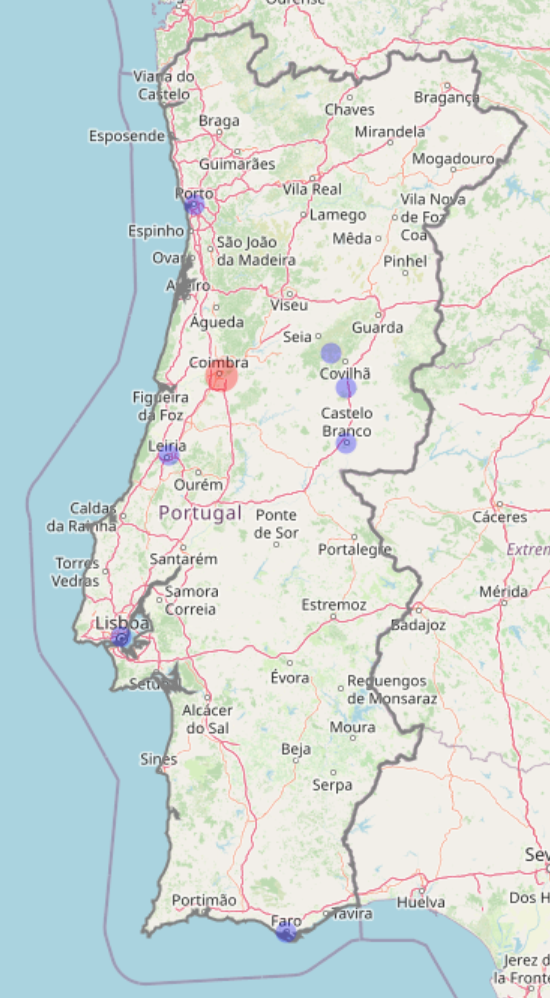
\includegraphics[width=0.3\linewidth]{images/map_D_core_elements2.png}
    \caption{\footnotesize{Core study domain $\mathcal{D}_{core}$ defined by Portugal region $\mathcal{R}_{pt}$ and the inner target points $\mathcal{P}_{pt,i}$.  }}
    \label{fig:map_D_core_elements}
\end{figure}


\subsubsection{Core Temporal Boundaries}

With the core spatial region $\mathcal{R}_{core}$ established for Mainland Portugal, $\mathcal{R}_{core} \equiv \mathcal{R}_{pt}$, the core study domain now requires a observational window here, represented as a temporal set $\mathcal{T}_{core}\subset\mathcal{T}$ describing the  fire season expected to occur and for which the satellite constellation shall have the performance assessed.

 We establish the full year of 2024 as the simulation core temporal  \inlineReq{R15}. Formally, $\mathcal{T}_{core}$ is defined as the continuous interval:
\begin{equation}
    \mathcal{T}_{core} = [t_{start_{2024}}, t_{end_{2024}}] \subset \mathcal{T}
\end{equation}
Where $t_{start_{2024}}$ corresponds to 2024-01-01 00:00:00 UTC and $t_{end_{2024}}$ to 2024-12-31 23:59:59 UTC.

\subparagraph{Portugal season markers}\hspace{0pt}

A detailed global study of fire season types was done by Zhang et al \cite{zhang_global_2025}. They used satellite-based Moderate Resolution Imaging Spectroradiometer (MODIS) burned area records (2001–2022) to classify global fire season types by the number of peaks, or modals, within a year. Globally, three fire season categories were identified: unimodal (31.25\%), bimodal (52.07\%), and random (16.69\%), as shown in Fig. \ref{fig:fire_season_types} and Fig. \ref{fig:map_global_fire_season_types}. Unimodal fire seasons occur mainly in boreal and tropical zones and last about 2.7 months, whereas temperate ecosystems typically have longer, bimodal fire seasons (~3 months) with two peaks per year. Portugal is classified as a temperate ecosystem with a bimodal fire season type.

To define the core study fire Season in Portugal, one can follow the definition of fire season presented in Fig. \ref{fig:fire_season_types}, where the bimodal general annual fire activity curve defines the day of year of the fire season onset $t_{\text{start}}$, two fire activity peaks instants $t_{\text{peak},1}$ and $t_{\text{peak},2}$,  finalizing with $t_{\text{end}}$. 

A survey of the fire-season marker maps (Fig.~\ref{fig:fire_season_start_end}--Fig.~\ref{fig:fire_season_start2_end2}) indicates moderate spatial heterogeneity across Portugal. For mission-level analysis, we therefore adopt indicative bounds that conservatively cover the earliest onset, the two dominant August peaks, and the late-season decay into February. The resulting marker set for a season year  is summarized in Table~\ref{tab:pt_fire_season_bounds}.

\subparagraph{Critical observational reference for the constellation}\hspace{0pt}

Portugal's fire season starts in March, with increasing fire activity peaking in summer. This is the critical observation period for the constellation, which has two main intense peaks in the first week of August and around the third week. The constellation shall have the best coverage in this month, with August 18 as the main fire peak reference \inlineReq{R16}. 
\begin{equation}
    t_{\text{peak fire ref}} = \text{ August 18th }
    \label{eq:peak_fire_ref_day}
\end{equation}
After this period of faster pyrodynamics, the season extends with decreasing intensity until fading in February of the next year. 


\begin{table}[ht]
\centering
\caption{\footnotesize{Definition of the Core Temporal Boundaries $\mathcal{T}_{core}$ for Portugal, detailing the two phenomenological sub-periods and peaks based on Day-of-Year (DOY).}}
\label{tab:pt_fire_season_bounds}
\renewcommand{\arraystretch}{1.2}
\begin{tabular}{lll p{5.5cm}}
\toprule
\textbf{Season Marker} & \textbf{Symbol} & \textbf{Date: (DOY)}& \textbf{Interpretation} \\
\midrule
Start fire subperiod 1 
& $t_{start,1}$
& Mar 11 ($\sim 70$)
& Earliest onset of fire activity. \\

1th peak& $t_{peak,1}$
& Aug 08 ($\sim 220$)
& First local peak of the bimodal cycle. \\

End fire subperiod 1 
& $t_{end,1}$
& Aug 13 ($\sim 225$)
& Transition to the core intensity period. \\

\midrule

Start fire subperiod 2 
& $t_{start,2}$
& Aug 13 ($\sim 225$)
& Onset of the critical design period. \\

2th peak& $\mathbf{t_{peak,2}}$
& \textbf{Aug 18 ($\sim 230$)}
& \textbf{Strongest seasonal peak. Critical design point.} \\

End fire subperiod 2 
& $t_{end,2}$
& Feb 09 ($\sim 40^*$)
& Latest tail end (referring to the subsequent year). \\
\bottomrule
\end{tabular}
\end{table}


\begin{figure}[H]
    \centering
    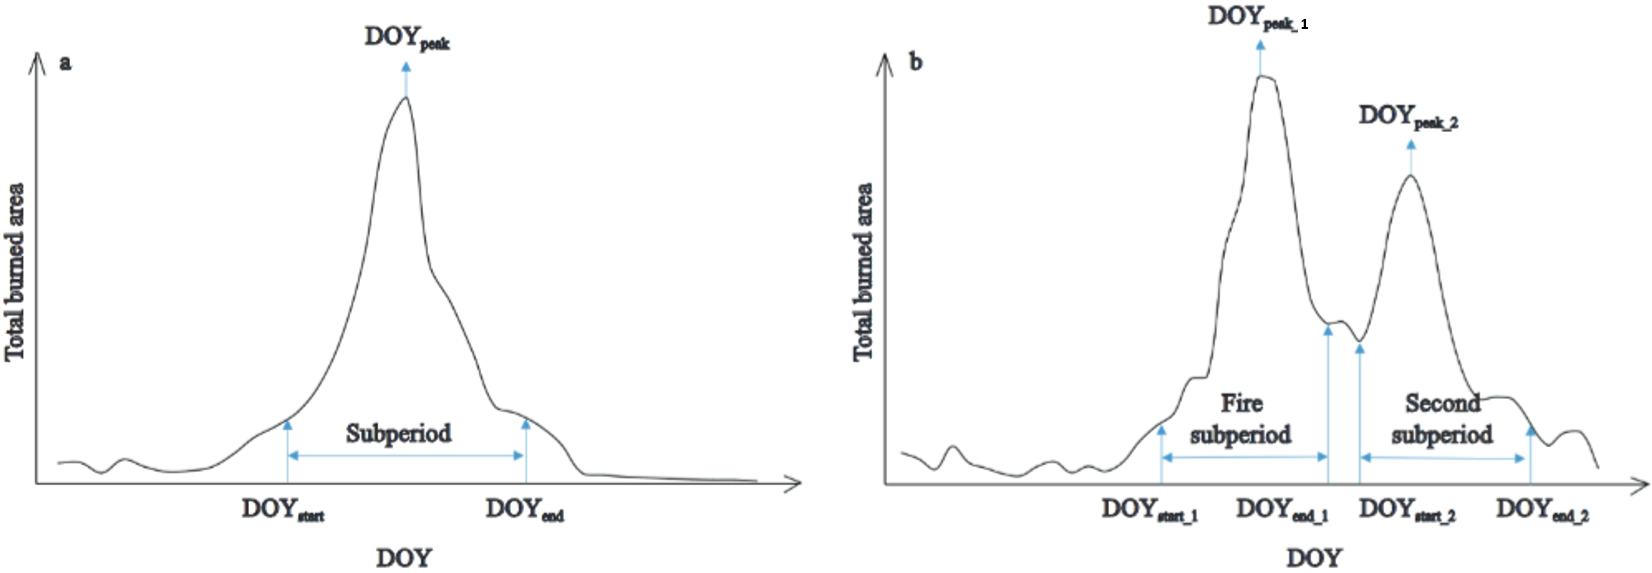
\includegraphics[width=1\linewidth]{images/fire_season_types.png}
    \caption{\footnotesize{The schematic diagram of unimodal (a) and bimodal (b) fire season types. The fire season starts on the day of year $\mathrm{DOY}_{\text{start}}$, it has peaks $\mathrm{DOY}_{\text{peak}}$, and ends on $\mathrm{DOY}_{\text{end}}$. \protect\footnotemark}}
    \label{fig:fire_season_types}
\end{figure}


\footnotetext{\label{fn:Zhang2025}Adapted from Zhang \emph{et al.} (2025)~\cite{zhang_global_2025}.}


\begin{figure}[H]
    \centering
    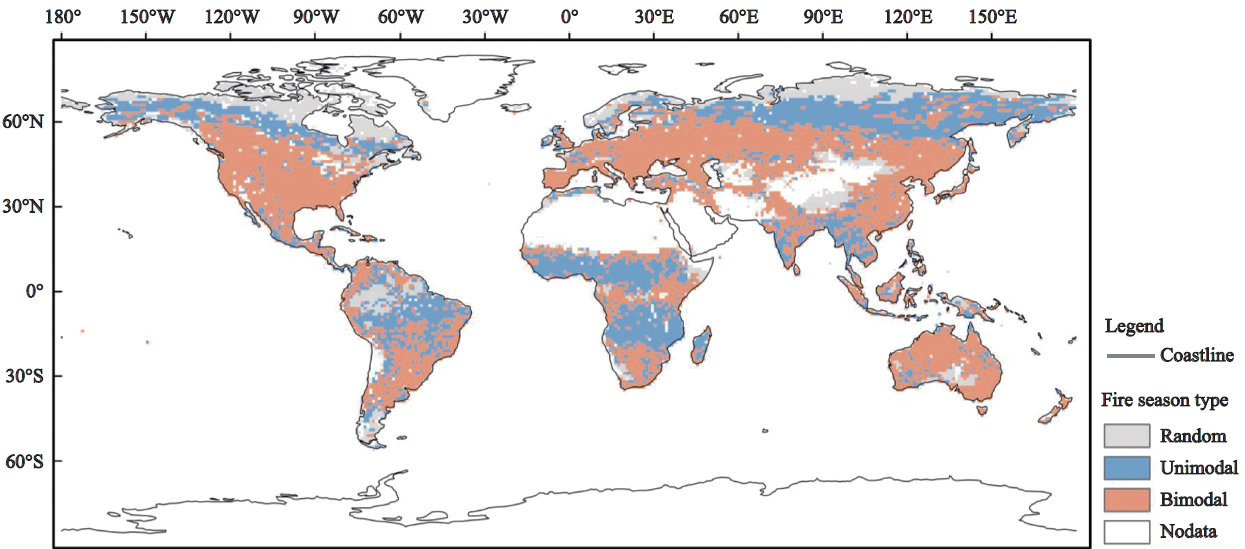
\includegraphics[width=0.65\linewidth]{images/map_global_fire_season_types.png}
    \caption{\footnotesize{Global distributions of fire season types from 2001 to 2022.  \textsuperscript{\ref{fn:Zhang2025}}}}
    \label{fig:map_global_fire_season_types}
\end{figure}

% \begin{figure}[H]
%     \centering
%     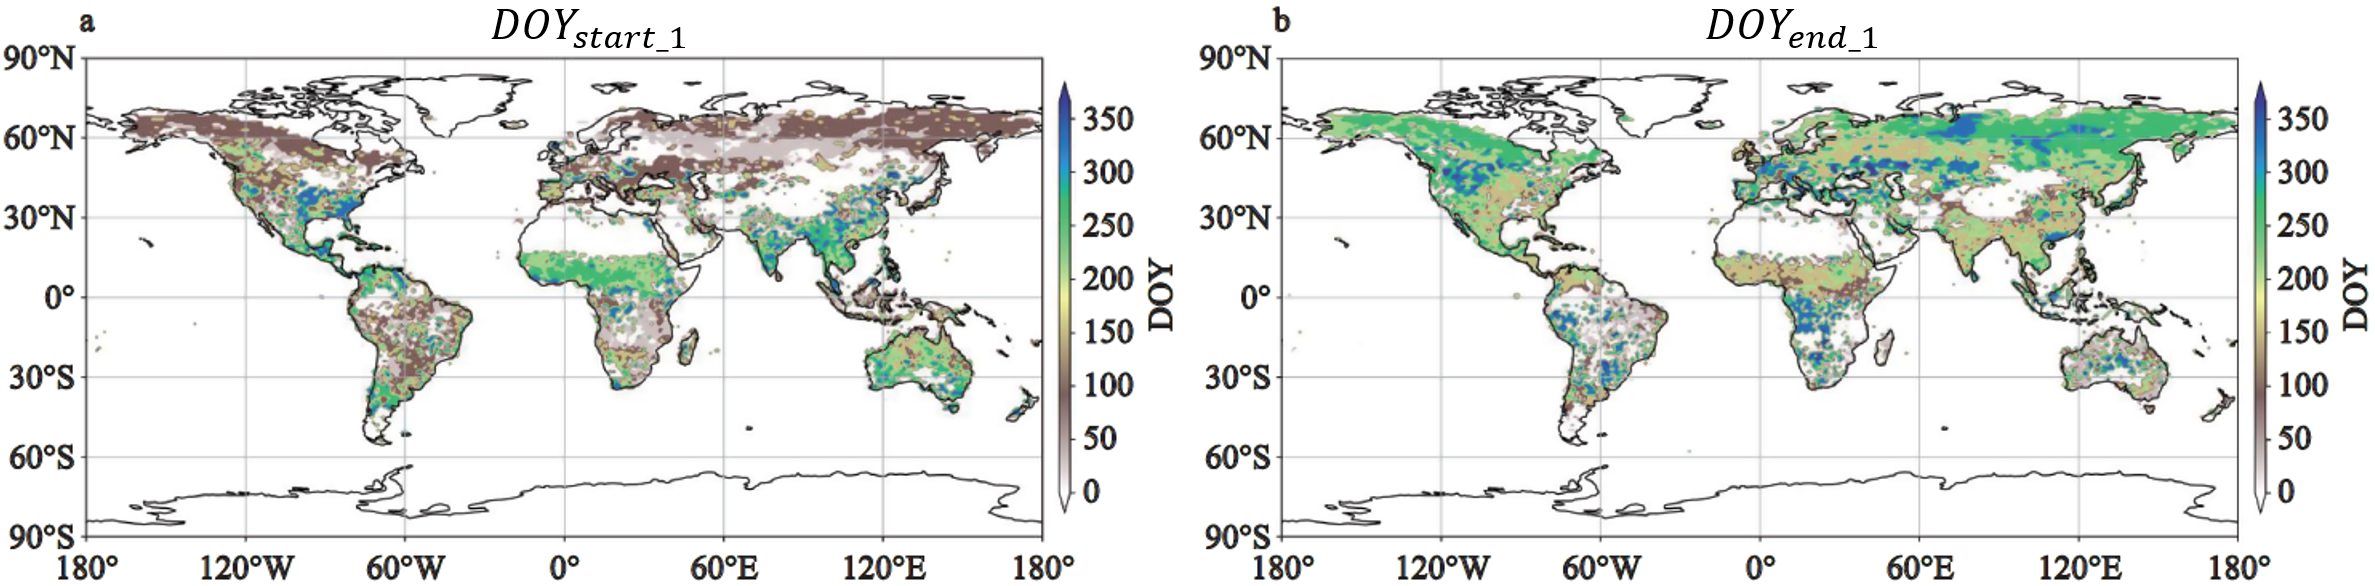
\includegraphics[width=0.9\linewidth]{images/fire_season_start1_end1.png}
%     \caption{\footnotesize{Global distributions of the fire season first subperiod (see Fig. \ref{fig:fire_season_types})  start day of year $\mathrm{DOY}_{\text{start 1}}$  (a) and end $\mathrm{DOY}_{\text{end 1}}$ (b).  \textsuperscript{\ref{fn:Zhang2025}}}}
%     \label{fig:fire_season_start_end}
% \end{figure}

% \begin{figure}[H]
%     \centering
%     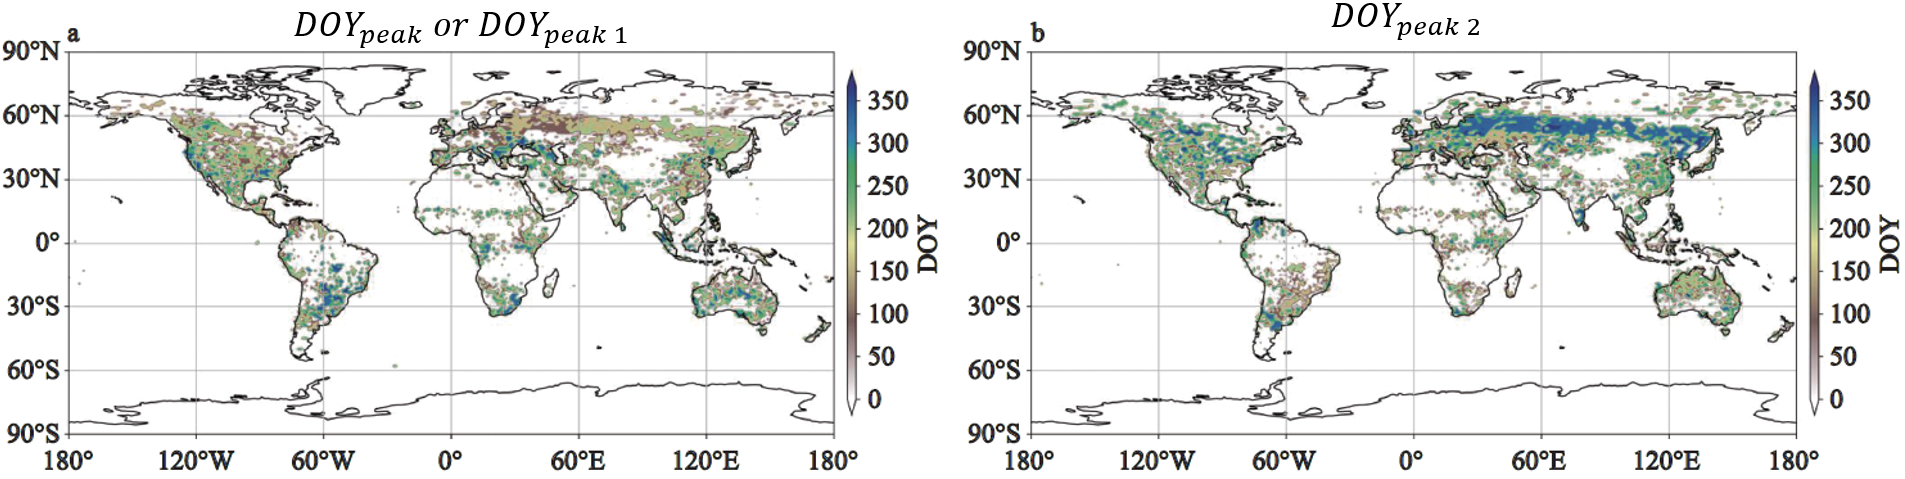
\includegraphics[width=0.9\linewidth]{images/fire_season_peaks.png}
%     \caption{\footnotesize{Global distributions of the peak start day of year $\mathrm{DOY}_{\text{peak} 1}$ in the first subperiod (a) and second subperiod $\mathrm{DOY}_{\text{peak}  2}$(b) of fire season from 2001 to 2022. See Fig. \ref{fig:fire_season_types} about subperiods.  \textsuperscript{\ref{fn:Zhang2025}}}}
%     \label{fig:fire_season_peaks}
% \end{figure}

% \begin{figure}[H]
%     \centering
%     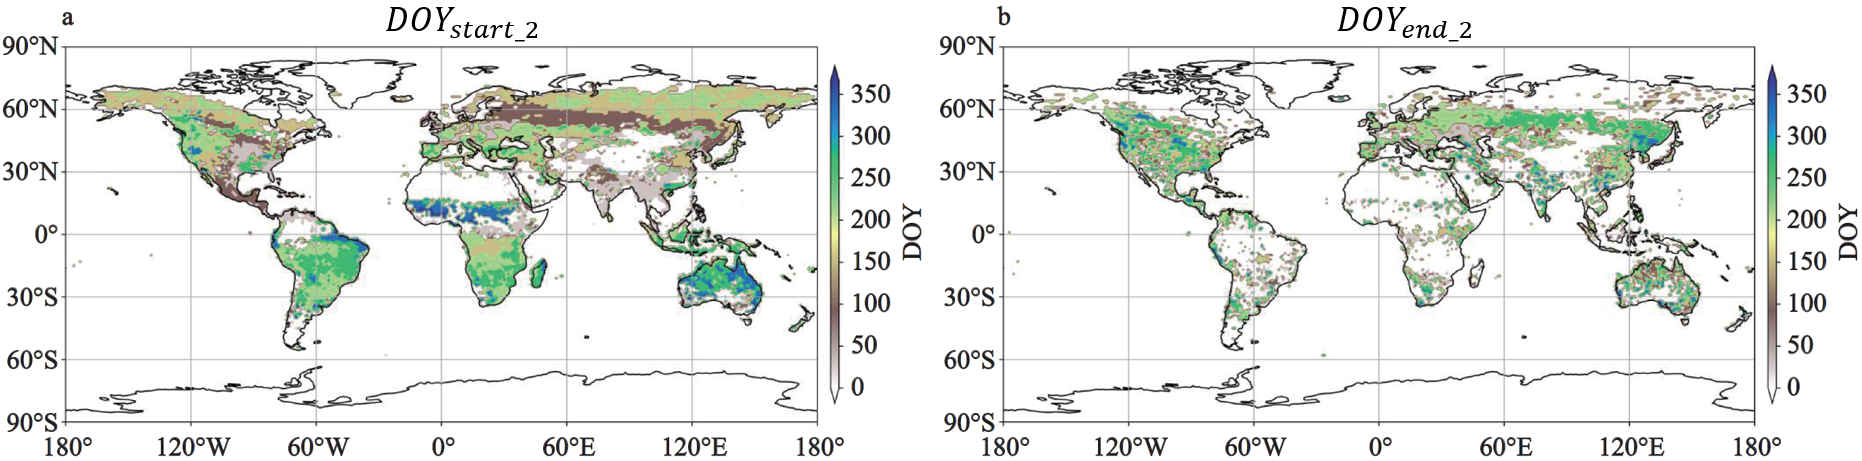
\includegraphics[width=0.9\linewidth]{images/fire_season_start2_end2.png}
%     \caption{\footnotesize{Global distributions of the fire season second subperiod (see Fig. \ref{fig:fire_season_types})  start day of year $\mathrm{DOY}_{\text{start 2}}$  (a) and end $\mathrm{DOY}_{\text{end 2}}$ (b).  \textsuperscript{\ref{fn:Zhang2025}}}}
%     \label{fig:fire_season_start2_end2}
% \end{figure}

% \begin{figure}[ht]
%   \centering
%   \fbox{%
%     \begin{minipage}[c][1cm][c]{0.9\linewidth}
%       \centering \textit{Figure placeholder}
%     \end{minipage}%
%   }
%   \caption{TODO: Add histogram of active fire in the GOEs dataset for portugal and identify the peaks, connect it to the global domain if makes sense}
%   \label{fig:placeholder_text}
% \end{figure}


\subsection{Generalized Study Domain}
\label{sec:generalized_study_domain}

This section details the properties of the Global Study Domain $\mathcal{D}_{global}$, establishing its spatial region elements $\mathcal{R}_{global}$ and temporal boundaries $\mathcal{T}_{global}$. Formally, the domain is defined as the Cartesian product of these sets:
\begin{equation}
    \mathcal{D}_{global} = \mathcal{R}_{global} \times \mathcal{T}_{global} \subset \mathcal{M}
\end{equation}

\subsubsection{Global Spatial Element}

To construct the global spatial definition, we extend the previous topological concepts of the Core Domain. However, unlike $\mathcal{R}_{core}$, which is bounded by static geopolitical borders (Mainland Portugal), the global region $\mathcal{R}_{global}$ is defined by phenomenological boundaries, specifically, the probability of fire occurrence on different types of biomass and climate \inlineReq{R17}.

We designate this spatial object as the Earth's Fire-Prone Region Target\textbf{ $\mathcal{R}_{\oplus_{FPR}}$}. Mathematically, it is defined not as a single contiguous shape, but as the union of all disjoint surface patches $S_k$ on the planetary ellipsoid that have fire-prone characteristics:

\begin{equation}
    \mathcal{R}_{global} \equiv \mathcal{R}_{\oplus_{FPR}} = \bigcup_{k} S_k  \mid  \text{Class}(S_k) \in \mathcal{C}_{fire}
\end{equation}
Where $\mathcal{C}_{fire}$ represents the set of valid fire-prone regions classifications.

\subsubsection{Earth's Fire-Prone Regions Targets ($\mathcal{R}_{\oplus_{FPR}}$)} \hspace{0pt}
\label{sec:earths_frp_targets}

The boundaries of these surface $S_k$ are determined by the fire-climate classes derived from historical satellite data (as seen in Fig. \ref{fig:fire_prone_global_now_future}), methodology proposed by Senande-Rivera et al. \cite{senande-rivera_spatial_2022}. Consequently, $\mathcal{R}_{\oplus_{FPR}}$ acts as a spatial filter, restricting the mission analysis to relevant latitudes and ecosystems (e.g., Mediterranean, Savanna, Temperate) while excluding non-flammable regions (e.g., rainy regions, deserts, oceans, ice sheets). 

\begin{figure}
    \centering
    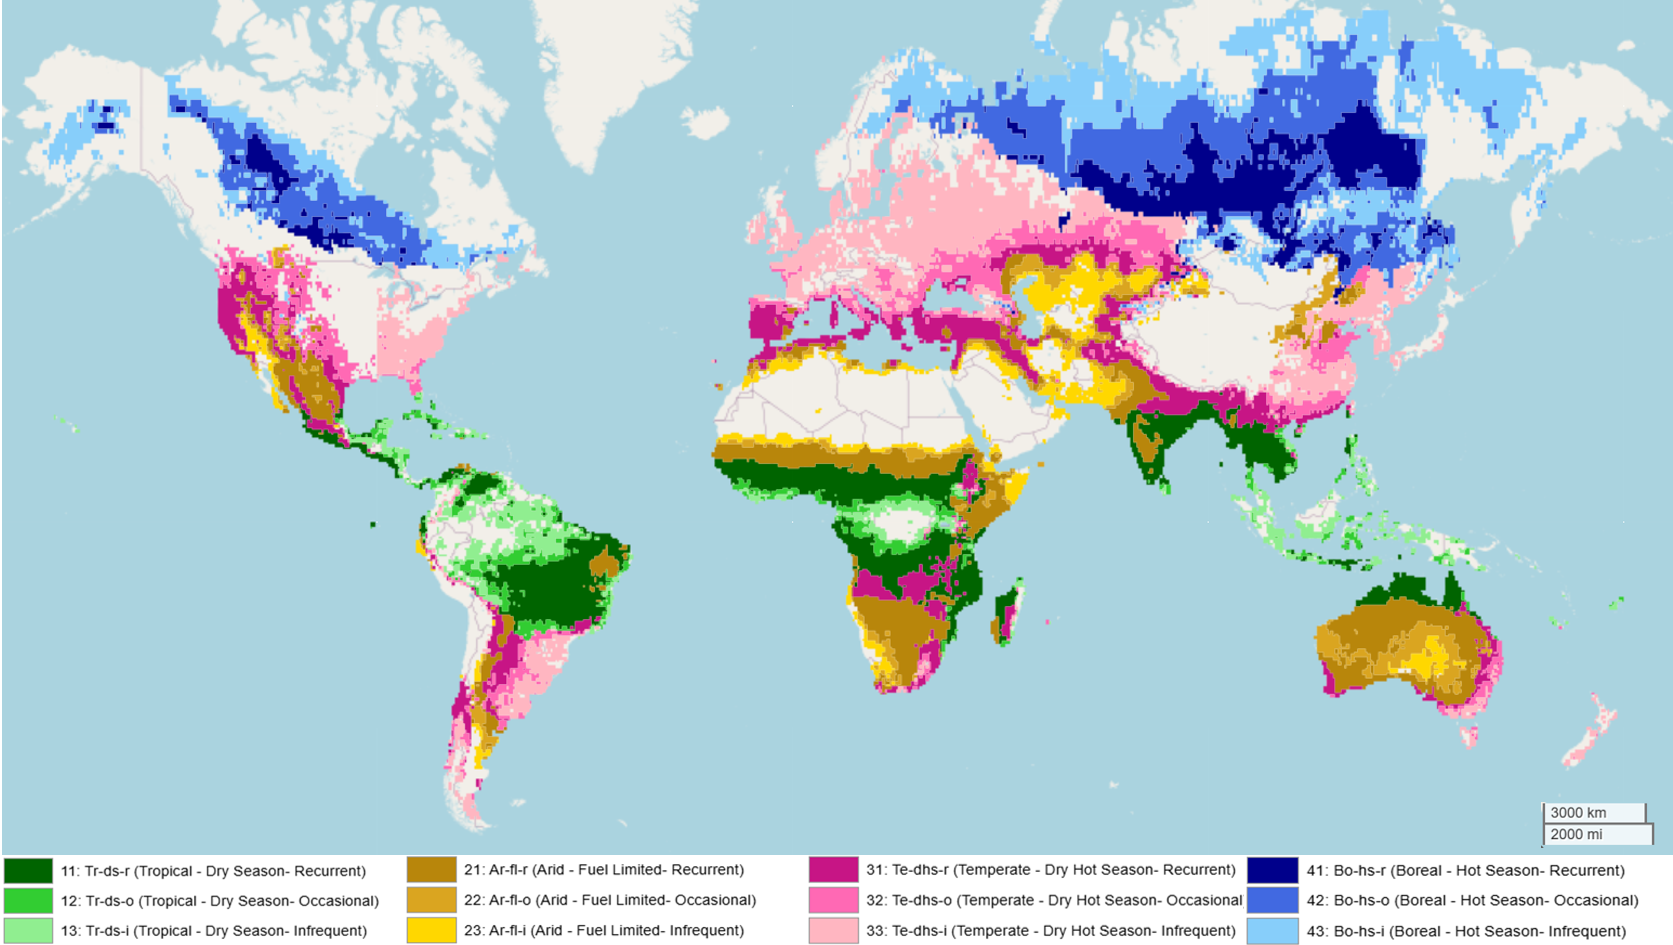
\includegraphics[width=1\linewidth]{images/map_earths_fireprone_region_targets.png}
    
    \caption{\footnotesize{\textbf{Spatial definition of the Earth's Fire-Prone Regions Target ($\mathcal{R}_{\oplus_{FPR}}$).} 
    The map visualizes the spatial element of the generalized study domain $\mathcal{R}_{global}$ as the union of all surface patches $S_k$ exhibiting valid fire-prone characteristics. Data is reconstructed from the \texttt{FC.nc} dataset provided by Senande-Rivera et al. \cite{senande-rivera_spatial_2022, senanderivera_fireclimate_2022}. The color coding corresponds to the specific fire-climate regimes $\alpha$ (e.g., \textit{Te-dhs-r}) defined in the taxonomy, stratified by climate (Tropical - Dry Season, Arid - Fuel Limited, Temperate - Dry Hot Season, Boreal - Hot Season), and fire frequency (Recurrent, Occasional, Infrequent). This spatial mask serves as the spatial operational filter for the constellation's global coverage analysis.}}
    
    \label{fig:map_earths_fire_prone_region_targets}
\end{figure}

\subparagraph{Classification Taxonomy}\hspace{0pt}

The classification assigns a descriptor to each region based on the nomenclature \texttt{[Climate]-[Type]-[Frequency]}.
First, regions are categorized into four primary climate regimes [Tropical, Arid, Temperate, Boreal] based on the Köppen–Geiger criteria. Then, specific fire thresholds are applied to identify the dominant phenomenological driver of fire activity (e.g., limited fuel vs. dry season). The intersection of these climatic and fire conditions defines the four primary classes presented bellow:

\begin{itemize}
    \item \textbf{Tr-ds (Tropical - Dry Season):} Regions driven by distinct dry seasons in tropical latitudes (e.g., Savannas).
    \item \textbf{Ar-fl (Arid - Fuel Limited):} Regions where fire activity is rare and constrained by available biomass rather than weather conditions.
    \item \textbf{Te-dhs (Temperate - Dry Hot Season):} Regions characterized by hot, dry summers (e.g., Mediterranean, Portugal). This is the primary analog to the Core Study Domain.
    \item \textbf{Bo-hs (Boreal - Hot Season):}High-latitude regions where fire activity is driven by seasonal heat waves and snow-melt timing.
\end{itemize}



\subparagraph{Frequency (Intensity)} \hspace{0pt}

Crucially for the satellite mission design of a fast wildfire constellation is the knoledge of the regions with higher frequency of fire. To assist on this goal, each climatic class is subdivided by intensity, defined by the number of \textit{Fire Prone Years (FPY)} per decade. This creates a hierarchy of observation priority:

\begin{enumerate}
    \item \textbf{Recurrent (r):} Regions with $> 7 FPY$/decade. These are high-priority targets requiring consistent monitoring if the coverage allows it depeding on the latitude.
    \item \textbf{Occasional (o):} Regions with $3 < FPY\text{/decade} \leq 7$.
    \item \textbf{Infrequent (i):} Regions with $0 < FPY\text{/decade} \leq 3$.
\end{enumerate}

\subparagraph{Operational Definition of the Global Target} \hspace{0pt}

For the purpose of this mission simulation, the generalized study domain $\mathcal{R}_{global}$ extends to all fire frequency subclasses, Recurrent (r), Occasional (o), Infrequent (i), as these represent locations where a dedicated constellation adds significant value for recurrent and intense fires, and also enables monitoring of sensitive regions, such as deforestation fronts, preservation areas, where fire activity is not yet as frequent \inlineReq{R18}.
Therefore, the valid set of target classes is defined as:
\begin{equation}
    \mathcal{C}_{fire} = \{ \text{Tr-ds}, \text{Ar-fl}, \text{Te-dhs}, \text{Bo-hs} \} \times \{ r, o, i \}
\end{equation}
This targets were modeled by Senande-Rivera et al. and they made the file of the fire-climate classification available. This work is using the "FC.nc" to reproduce Rivera work as the $\mathcal{R}_{\oplus_{FPR}}$  \cite{senanderivera_fireclimate_2022}. The domain mask of $\mathcal{R}_{\oplus_{FPR}}$ are mapped into raster file which pixels values encompasses codes such as \textit{31 (Te-dhs-r)}, the class containing Portugal, and extends to others like \textit{11 (Tr-ds-r)} or \textit{42 (Bo-hs-o)}, providing a comprehensive global map of fire-prone targets as seen in Fig. \ref{fig:map_earths_fire_prone_region_targets}.

% \subparagraph{Nomenclature (Index Notation)}

% To facilitate precise referencing of specific fire regimes throughout this work, we adopt a notation style analogous to tensor calculus. The specific fire-climate class $\alpha \in \mathcal{C}_{fire}$ of a target region is denoted as a superscript index on the region variable:
% \begin{equation}
%     \mathcal{R}_{\oplus_{FPR}}^{\alpha}
% \end{equation}
% For example, the specific subset of regions corresponding to the Portuguese profile (Temperate-dry hot season, recurrent) is denoted as $\mathcal{R}_{\oplus_{FPR}}^{\text{Te-dhs-r}}$.

\subsubsection{Global Temporal Boundaries}

While the spatial domain $\mathcal{R}_{global}$ is defined by static climatological likelihoods connected to historical burned areas, the temporal domain $\mathcal{T}_{global}$ requires a deterministic temporal space populated by active fire events. These serve as the ground truth references to verify the satellite dynamic constellation performance.

Before defining this global fire history, we establish the temporal bounds. We select the \textbf{Full Calendar Year of 2024} as the simulation baseline \inlineReq{R19}. Formally, $\mathcal{T}_{global}$ is defined as the continuous interval:

\begin{equation}
    \mathcal{T}_{global} = [t_{start}^{2024}, t_{end}^{2024}] \subset \mathcal{T}
\end{equation}
Where $t_{start}^{2024}$ corresponds to 2024-01-01 00:00:00 UTC and $t_{end}^{2024}$ to 2024-12-31 23:59:59 UTC.

\paragraph{Reference Active Fire Events ($\Upsilon_{fires}$)} \hspace{0pt}

A key methodological contribution of this work is the use of an \textbf{observation-based, high-cadence global active-fire event database} (FireDS) as the verification reference, instead of relying on stochastic fire-generation models. To verify rapid-detection performance ($t_{revisit} \leq 30$~min; \reqRef{R7}), the reference dataset must be time-sampled more finely than the constellation revisit period \inlineReq{R20}. In particular, letting $\Delta t_{FireDS}$ denote the active fire dataset sampling interval, the following condition is required:
\begin{equation}
    \Delta t_{FireDS} \leq t_{revisit}
\end{equation}
Formally, $\mathcal{O}_{FireDS}$ is defined as the collection of active fire phenomena units $\Psi_n$ contained in the FireDS source. The set $\Upsilon_{fires}$ is defined as the subset of reference active fire events from this database that fall within the mission's global space-time domain:
\begin{equation}
    \Upsilon_{fires} = \mathcal{O}_{FireDS} \cap \mathcal{D}_{global}
\end{equation}
This filters the dataset for events relevant to the study constraints:
\begin{equation}
    \Upsilon_{fires} = \{ \Psi_n(\mathbf{r}, t, P_{frp}) \in \mathcal{O}_{FireDS} \mid \mathbf{r}_n \in \mathcal{R}_{\oplus_{FPR}} \wedge t_n \in \mathcal{T}_{global} \}
\end{equation}
where each element $\Psi_n$ represents a unique active fire event characterized by a coordinate vector $\mathbf{r}$, epoch $t$, and Fire Radiative Power (FRP) intensity $P_{frp}$.

\subparagraph{Fire Data Source: FIRMS Geostationary Dataset} \hspace{0pt}
\label{sec:firms_dataset}
To populate $\Upsilon_{fires}$, this work utilizes NASA's Fire Information for Resource Management System \textbf{(FIRMS) global geostationary active fire} (FIRMS$_{FireDS}$) dataset \cite{davies_geostationary_2024}. This dataset was released recently in June 2024; to the author's knowledge, the use of FIRMS$_{FireDS}$ for satellite constellation design is novel in the literature. 

Unlike Low-Earth Orbit (LEO) sensors (e.g., VIIRS, Sentinel-2, MODIS) which provide only limited daily snapshots (approx. 1, 2, or 6), this dataset integrates Near Real-Time (NRT) data from five geostationary weather platforms to create a continuous global fire record (Table \ref{tab:geo_satellites}). 

These five geostationary satellites (altitude $\approx 35,900$ km) provide active fire products with near-global coverage, excluding only the polar regions, as seen in Fig \ref{fig:firms_geostationary_sats}. The network comprises Meteosat (ESA), Himawari (Japan), INSAT (India), and GOES-East/West (USA).

% \begin{figure}[H]
%     \centering
%     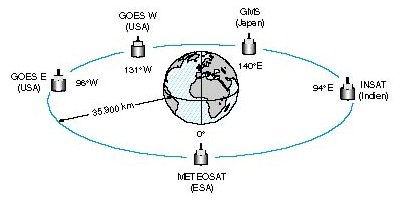
\includegraphics[width=0.5\linewidth]{images/Meteosat_geosats.jpg}
%     \caption{\footnotesize{Five identical geostationary satellites are arranged in a constellation along the equator. These include Meteosat (ESA), Himawari (JAXA), INSAT (ISRO), and GOES-E / GOES-W (NOAA). Together, they provide new images of global weather conditions every half hour, excluding the Polar Regions \cite{_esa_2013}.}}
%     \label{fig:Meteosat_geosats}
% \end{figure}
% \begin{figure}[H]
%     \centering
%     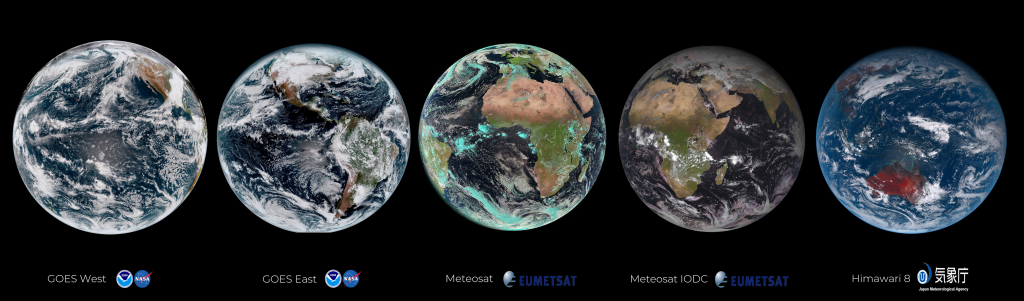
\includegraphics[width=0.8\linewidth]{images/full_earth_disk_image_GOES16_18_Meteosat11_9_Himawari9.png}
%     \caption{\footnotesize{Earth's full disk image by the geostationary satellite capable of fire detection. GOES W \& E, Meteosat 9 \& 11, Himawai 9.\cite{_algorithm_} }}
%     \label{fig:earth_full_disk_geosats}
% \end{figure}
\begin{figure}
    \centering
    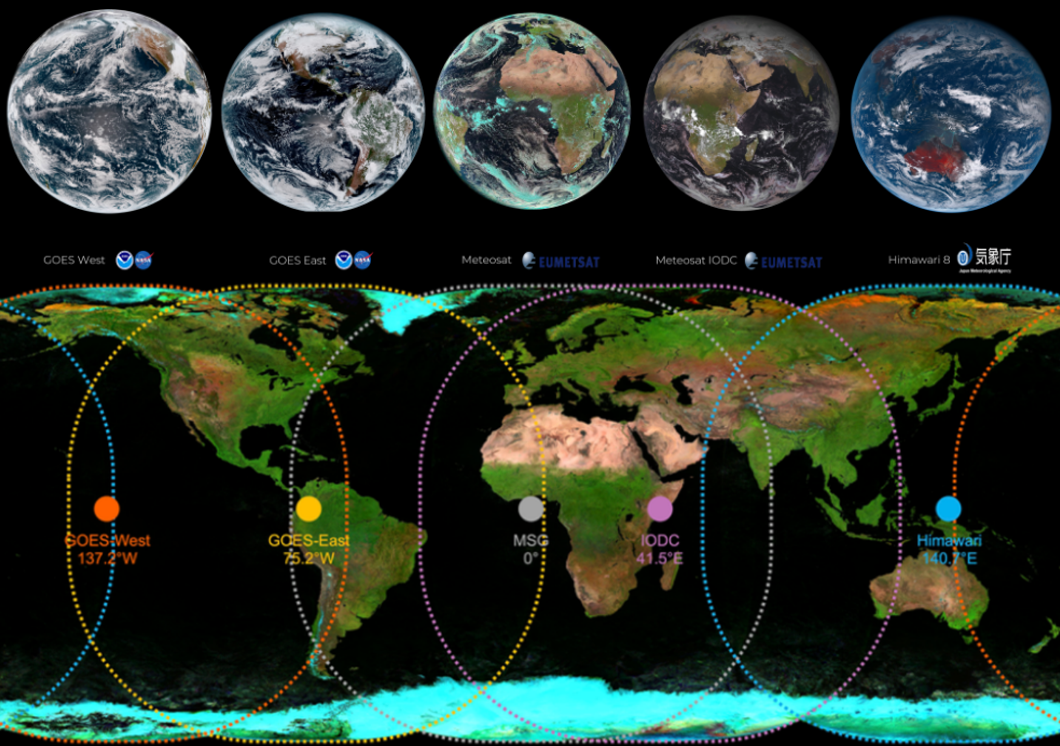
\includegraphics[width=1\linewidth]{images/FIRMS_GEO_sats_Earth_Disks.png}
    \caption{\footnotesize{Top: Earth's full disk image by the geostationary satellite capable of fire detection. GOES W \& E, Meteosat 9 \& 11, Himawai 9.\cite{_algorithm_} Bottom: Spatial coverage of five geostationary satellites used to achieve near real-time (10--15 min) active fire detection in FIRMS. This is the dataset used to populate the reference active fire events $\Upsilon_{ref}$ belonging to the global study temporal domain $\mathcal{T}_{global}$ \cite{davies_geostationary_2024}.}}
    \label{fig:firms_geostationary_sats}
\end{figure}


This multi-satellite geostationary constellation layer (GeoLayer) provides global coverage with a temporal resolution of $\Delta t_{FireDS} \approx 10-15$ minutes; . This high-cadence system captures the evolution of fire intensity, serving as the necessary "High-Frequency Ground Truth" to validate whether the proposed LEO constellation layer architecture (LeoLayer) successfully captures the fire timeline during its active phase; \inlineReq{R21}.

\begin{table}
\centering
\caption{\footnotesize{Composition of the Global Reference Data Source (FIRMS Geostationary). These instruments define the "True Events" ($\Psi_n$) used to validate the simulation in the 2024 temporal window.}}
\label{tab:geo_satellites}
\renewcommand{\arraystretch}{1.2}
\begin{tabular}{l l l c}
\toprule
\textbf{Satellite Platform} & \textbf{Instrument} & \textbf{Coverage Area} & \textbf{Resolution ($\Delta t$)} \\
\midrule
\textbf{GOES-16} (East) & ABI & North/South America (East) & 10 min \\
\textbf{GOES-18} (West) & ABI & North/South America (West) & 10 min \\
\textbf{Meteosat-9/11} & SEVIRI & Europe, Africa, Indian Ocean & 15 min \\
\textbf{Himawari-8/9} & AHI & Asia, Pacific, Australia & 10 min \\
\bottomrule
\end{tabular}
\end{table}


\paragraph{GeoLayer Spatial Resolution and Geometry Considerations} 
\label{sec:geolayer_spatial_and_temporal_resolution}

While the GeoLayer FIRMS$_{FireDS}$ dataset provides near-real-time active-fire reference data, it imposes specific spatial constraints that must be accounted for. The nominal spatial resolution at the sub-satellite point (nadir) ranges from $GSD_{GeoLayer} \approx$ 2 km to 3 km, which is significantly coarser than that of LEO sensors like VIIRS (375 m) or the desired constellation spatial resolution of 6 m/pixel \reqRef{R7}; \inlineReq{R22}. Furthermore, at the large viewing angles of geostationary orbits, the pixel footprint undergoes geometric distortion, increasing substantially toward the poles \cite{davies_geostationary_2024}.

However, for the specific purpose of this mission analysis—validating the temporal detection latency—this coarse spatial resolution is not a limiting factor. The typical field of view (FOV) and footprint (swath) of the proposed LEO CubeSat sensors significantly exceed the uncertainty associated with a single geostationary pixel ($\text{Swath}_{LEO} \gg GSD_{GeoLayer}$). Thus, even if the exact sub-pixel location of the fire is unknown within the 2–4 km footprint, the event remains well-contained within the observational swath of the passing satellite. Therefore, the geostationary fast-but-coarse detection remains a valid ground truth for assessing whether the constellation intercepted the region during the active fire window.

\begin{figure}[H]
    \centering
    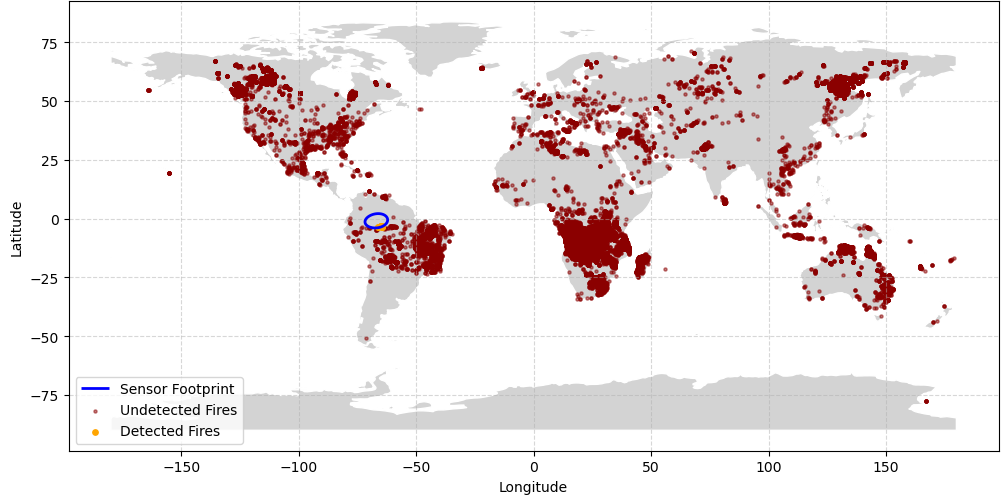
\includegraphics[width=1\linewidth]{images/map_viirs_active_fire_satellite_footprin_detection.png}
    \caption{\footnotesize{\textbf{Global distribution of Reference Fire Events ($\Upsilon_{ref}$) for 2024.} 
    The map illustrates the spatial aggregation of all active fire detections $\Psi_n$ derived from the FIRMS Geostationary dataset (GOES, Meteosat, Himawari) throughout the observation window $\mathcal{T}_{global}$. These discrete high-cadence events serve as the empirical ground truth for validating the constellation's detection latency.}}
    \label{fig:firms_geo_2024}
\end{figure}

\subparagraph{GeoLayer as Candidate Architectural Component} 
\label{sec:geolayer_candidate_architecture}
\hspace{0pt}

Beyond serving as a validation baseline, the high temporal cadence of the \textit{GeoLayer} also highlights its potential utility as an operational segment of the mission. Integrating these coarse GeoLayer rapid-fire alerts with the high-resolution capabilities of the \textit{LeoLayer} enables a viable "Tip-and-Cue" architecture strategy; \inlineReq{R23}. This cooperative multi-sensor layered approach, takes advantage of available public infrastructure (GeoLayer), providing a pathway to simultaneously satisfy the demanding, often conflicting requirements of rapid global revisit ($t_{revisit} \approx 30$ min) and high spatial detail ($GSD \approx 6$ m); see \reqRef{R7}, \reqRef{R8}. Therefore, the satellites indicated in table \ref{tab:geo_satellites}, which compose the FIRMS fire-alert, are identified as candidates for the GeoLayer architecture component for a global domain mission solution \inlineReq{24}. The formal trade-off analysis and detailed design of this hybrid architecture are presented in the Mission Architecture section.

\begin{figure}[H]
    \centering
    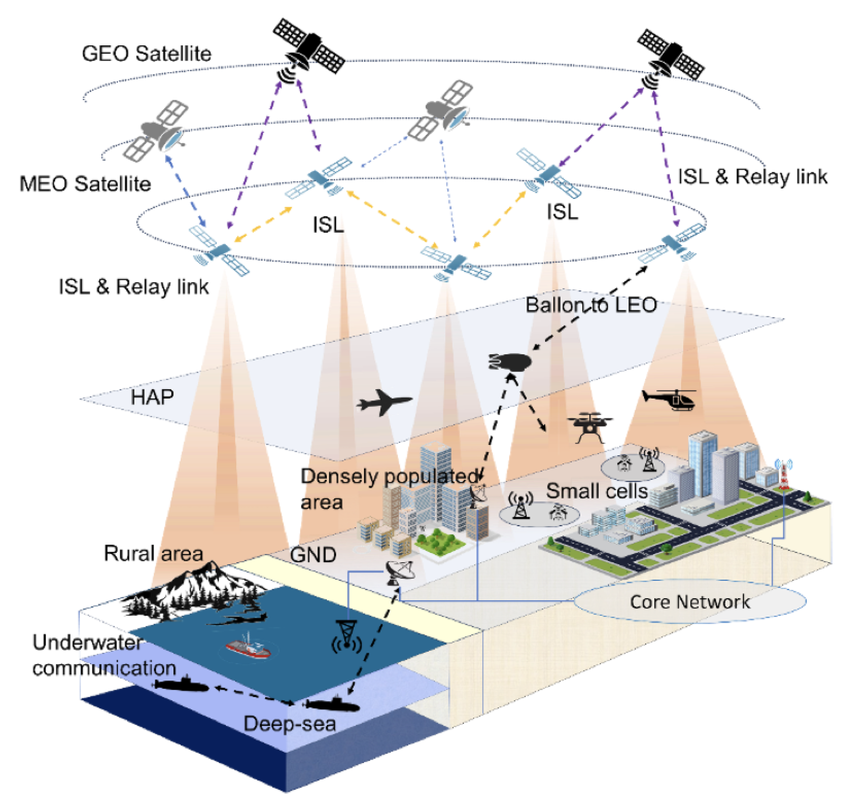
\includegraphics[width=0.85\linewidth]{images/tip-and-cue_architecture_example.png}
    \caption{\footnotesize{Example of tip-and-cue satellite communication architecture. Each sensor has unique advantages and disadvantages; combining and communicating these systems leads to higher temporo-spatial fidelity solutions impossible with separated units~\cite{_architecture_tipcue}.}}
    \label{fig:tip-and-cue_example}
\end{figure}

\subparagraph{GeoLayer New Generation Satellites} \hspace{0pt}
\label{sec:geolayer_new_gen}

New-generation geostationary satellites are emerging, improving spatial resolution and temporal detection capabilities. An example is \textbf{Meteosat-12} (formerly MTG-I1), the first of the Meteosat Third Generation Imager series. Declared fully operational in December 2024, this platform carries the Flexible Combined Imager (FCI), which enhances spatial resolution over Europe to \textbf{0.5 km - 2 km}, a marked improvement compared to the 3 km standard of the previous generation (MSG, GOES) \cite{_meteosat_2022}. 

\begin{figure}[H]
    \centering
    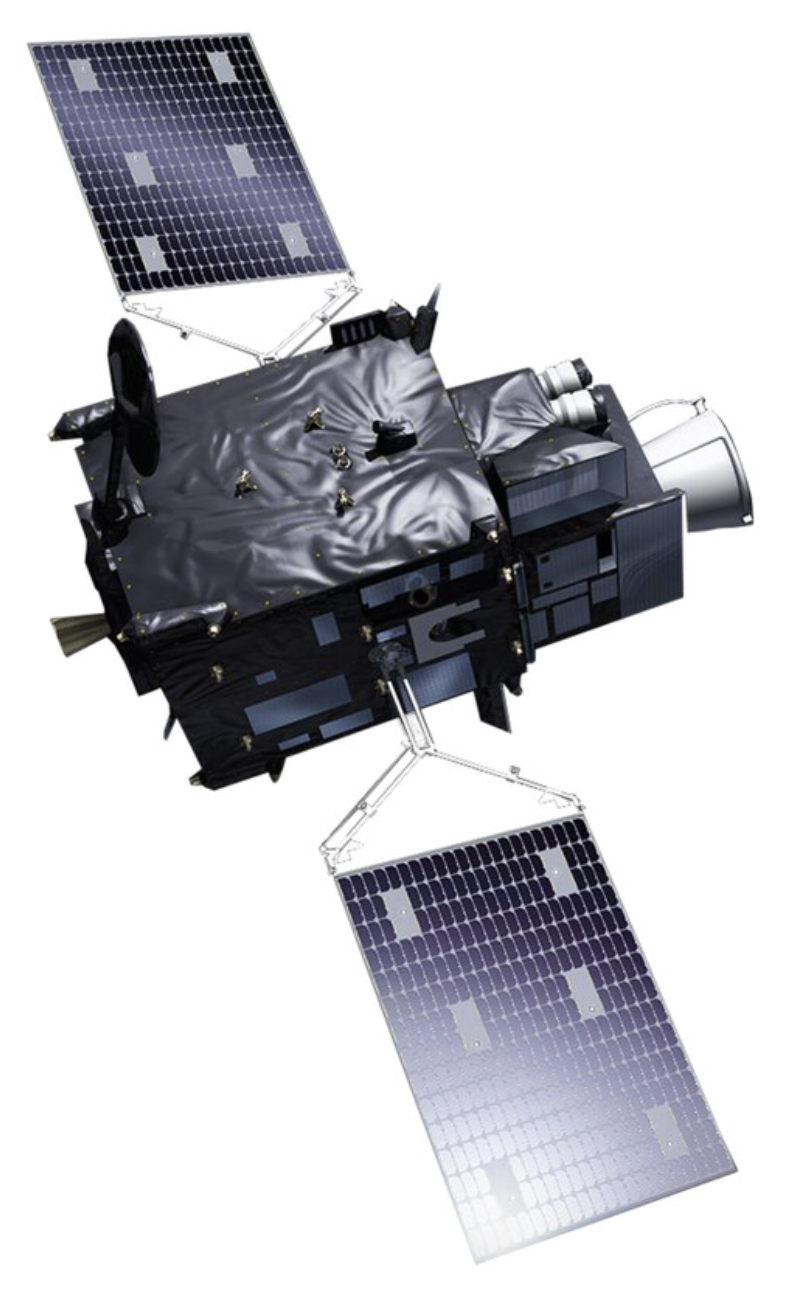
\includegraphics[width=0.15\linewidth]{images/meteosat12_render.png}
    \caption{\footnotesize{Meteosat-12,  Third Generation Geostationary Imager capable of 2.5min scan over European section with\textbf{ \textbf{0.5 km - 2 km}} GSD}}
    \label{fig:meteosat12_render}
\end{figure}

Furthermore, the MTG-I platform architecture introduces the capability for a \textbf{Rapid Scan Service (RSS)} of the European sector (Northern Quarter of Earth's disk) every \textbf{2.5 minutes} with all 16 spectral channels, significantly faster than the standard 10-minute Full Disk Scan \cite{eumetsat_rss_info, eumetsat_rss_2024}. The system also supports fire alerts and Fire Radiative Power (FRP) products, offering superior sensitivity for early event detection. 

\begin{figure}[H]
    \centering
    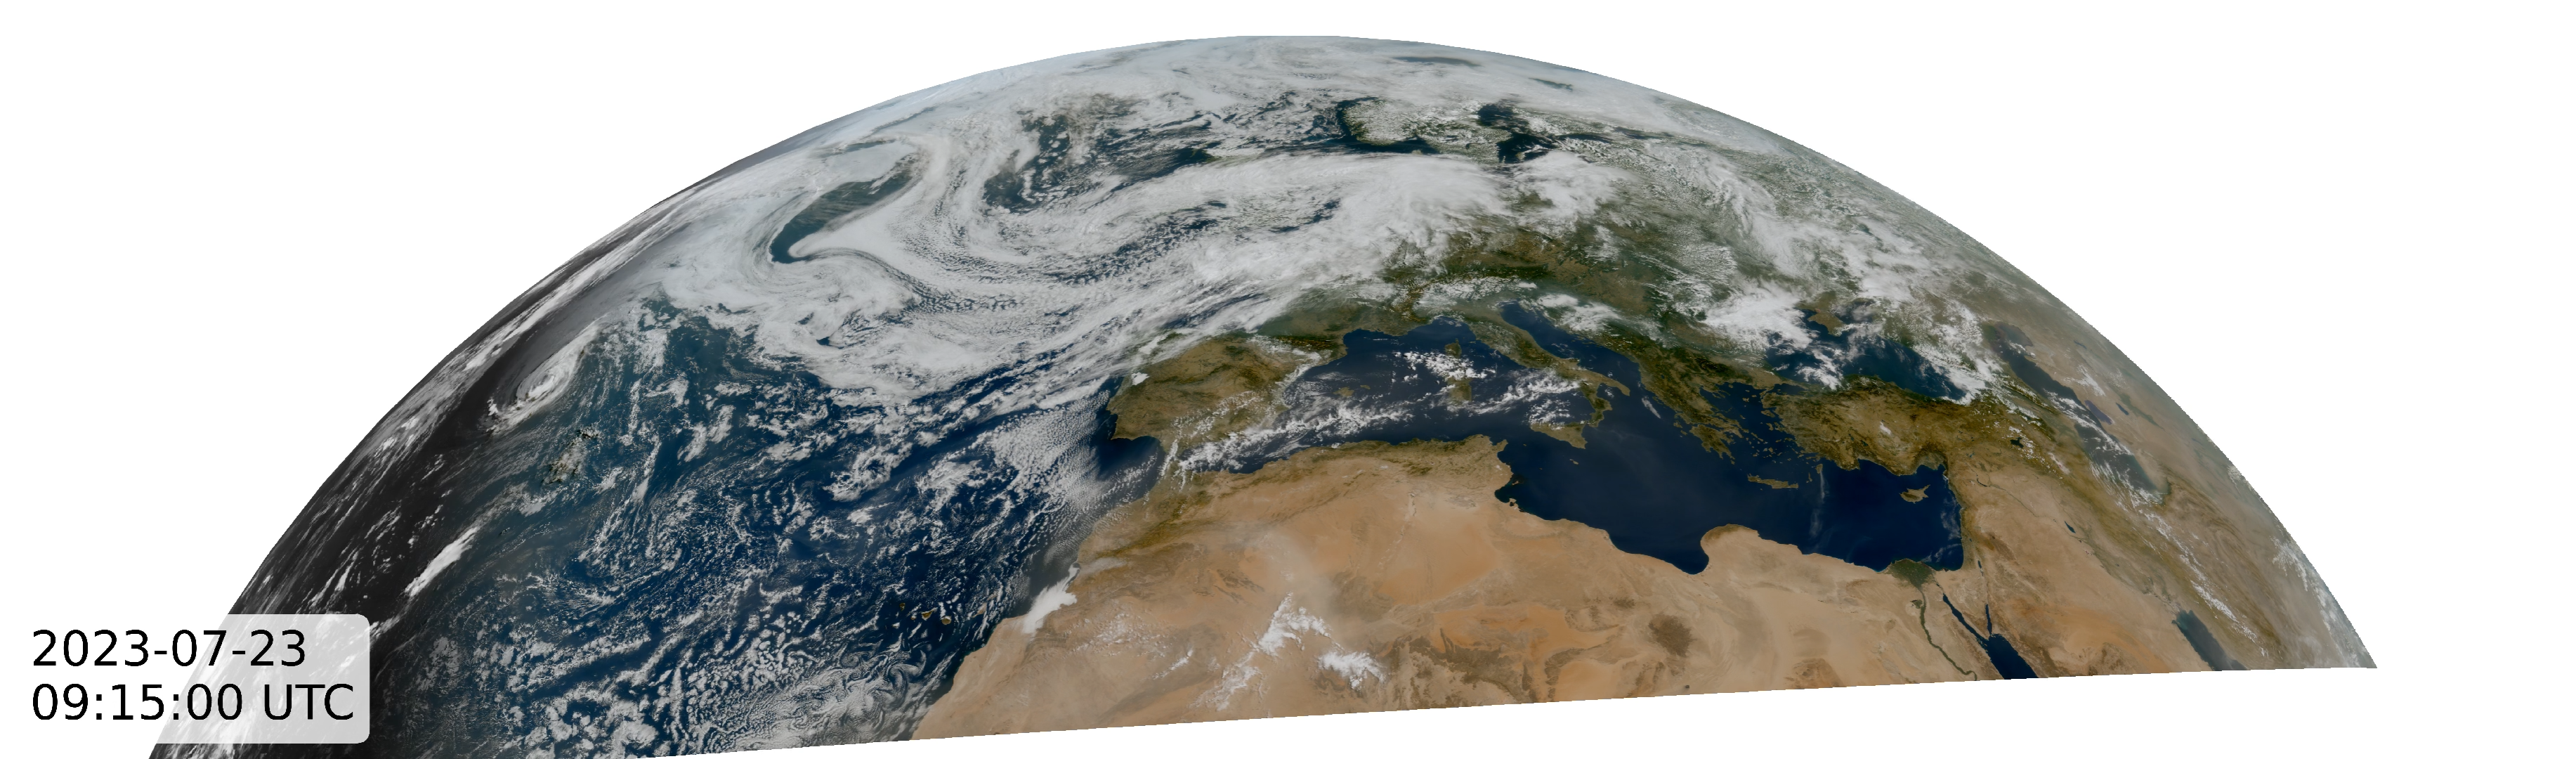
\includegraphics[width=1\linewidth]{images/meteosat12_rapid_scan_service_example.png}
    \caption{\footnotesize{Meteosat-12 Rapid Scan Service test dataset example. FCI True Colour RGB with night layer, animation with 2.5min repeat rate, 23 July 2023, 08:52:30 UTC-24 July 2023, 07:57:30 UTC Enter Caption. Video at \cite{eumetsat_rss_info}. }}
    \label{fig:meteosat12_rss}
\end{figure}

Looking ahead, the constellation will be completed by \textbf{Meteosat-14} (MTG-I2), which is scheduled for launch in \textbf{September 2026} \cite{eumetsat_planned_launches}. Following its commissioning, this platform will solidify the high-cadence architecture by assuming responsibility for the dedicated Rapid Scan Service (RSS) from the legacy fleet in \textbf{2027}.

Given these performance metrics, Meteosat-12 \& 14 are identified as strong candidates for the GeoLayer component over Europe \inlineReq{25}. However, a unified global dataset for this new, higher-fidelity geosat generation, spanning longitudes worldwide, does not yet exist. Therefore, for global performance analysis in this work, we will continue to use the established FIRMS Geolayer FIRMS$_{FireDS}$ dataset, which provides the global consistency required for the simulation.

%%% ----- Continue working


\section{Requirements Study Case Summary and Chapter Conclusion}
\label{sec:requirements-study-case-summary}

This section consolidates the study domain definitions from the preceding sections into traceable, design-level requirements. These requirements establish the spatial and temporal boundaries for the mission simulation, define the reference datasets for verification, and specify the architectural constraints for the satellite constellation assessment.

Detailed requirements derived in this chapter (R9--R25), covering the Core Study Domain, Global Study Domain, Reference Data, and Architecture constraints, are provided in Appendix~\ref{sec:app_req_ch2}.

In summary, this chapter has defined the two observational study domains that anchor the mission analysis. The Core Study Domain $\mathcal{D}_{core}$ fixes the spatial boundaries to mainland Portugal and the temporal bounds to its fire season centred on the August~18 peak, providing the primary evaluation context for the constellation. The Global Study Domain $\mathcal{D}_{global}$ extends coverage to all fire-prone regions classified by climate regime and fire frequency, using the FIRMS geostationary active-fire dataset as an observation-based, high-cadence verification baseline. Together, the spatial, temporal, and data-source definitions consolidated in requirements R9--R25 establish the inputs for the physical foundations of fire remote sensing developed in the next chapter.


% --- CHAPTER 3: The Physics of Fire Remote Sensing ---
\chapter{The Physics of Fire Remote
Sensing}\label{chapter-3-the-physics-of-wildfire-remote-sensing}

% \begin{quote}
% \textbf{Writing Guide \& Methodological Focus:}

% \begin{itemize}
% \item
%   \textbf{Objective:} To explain the fundamental science of \emph{how} a
%   fire can be "seen" from space. This chapter provides the physical
%   foundation for the sensor requirements and how they need to be
%   distributed over the constellation.
% \item
%   \textbf{Method:} Divide the physics into two parts: the source (the
%   fire) and the detection challenge (the observation).
% \item
%   \textbf{Caution:} Keep the physics focused and conceptual. Not
%   designing the sensor, but establishing the principles that dictate its
%   necessary characteristics.
% \item
%   \textbf{Checkpoint:} Does this chapter clearly explain \emph{why} a
%   satellite needs specific type of sensors to meet the
%   mission\textquotesingle s goals?
% \end{itemize}
% \end{quote}
The satellite constellation architecture configuration will depend on the distribution of satellite nodes across the orbital network and on the geometric constraints of each spacecraft's fire detectors. Therefore, the basic concept of fire remote detection from Earth orbit will be presented in this chapter to provide the necessary physical foundation for deducing mission requirements. 

\section{Physical Base of Remote Sensing}
\label{310-physical-base-of-remote-sensing}

A satellite sensor measures Electromagnetic (EM) energy within a given spectral band that reaches its aperture from a specific direction. This energy, reflected or emitted from a ground target, travels toward the detector. On this path, it interacts with the atmosphere, clouds, smoke, and other particles. The final energy flux measured will differ from the initial flux from the target due to these interactions. The fundamental radiometric quantity detected is the \textbf{radiance} $L$, defined below based on radiometric primitives.

\subsection{Radiometric primitives: irradiance, exitance, and radiance}
\begin{figure}
    \centering
    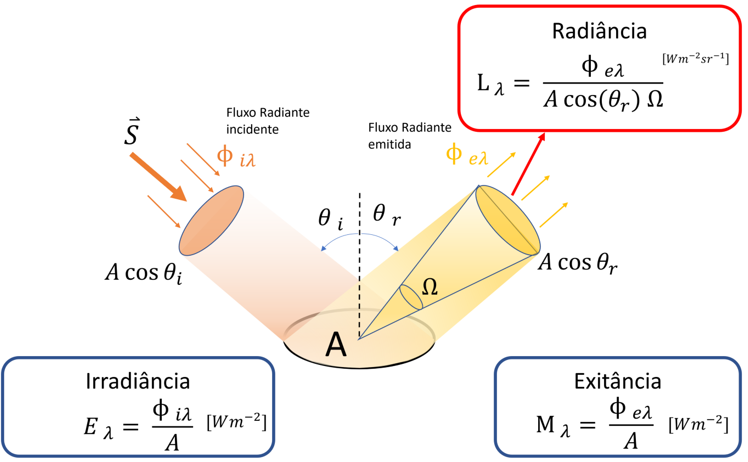
\includegraphics[width=0.75\linewidth]{images/remote_detection_principles.png}
    \caption{\footnotesize{Geometric definitions of the fundamental radiometric primitives. The diagram illustrates the distinction between the hemispherical fluxes of Irradiance ($E_\lambda$) and Exitance ($M_\lambda$), normalized by surface area $A$, versus the directional quantity of Radiance ($L_\lambda$), normalized by projected area $A \cos \theta_r$ and solid angle $\Omega$. Effects of atmospheric transmittance and path radiance are implicitly assumed in the propagation. }}
    \label{fig:remote_sense_radiometric_primitives}
\end{figure}

Consider the study domain $\mathcal{D}$ with a region target $\mathcal{R} \in \mathcal{F}_\oplus$ observed by a satellite as represented in Fig. \ref{fig:remote_sense_radiometric_primitives}. An elementary plane surface patch $S_j$, with $S_j \in \mathcal{R}$, has its area $A$ irradiated by electromagnetic radiation from the pointing vector $\vec{S}$ at an incidence angle $\theta_i$ with respect to the surface normal. Let $Q_{\lambda}$ be the radiant energy in a narrow spectral interval around wavelength $\lambda$ that crosses area $A$ within time $\Delta t$. The corresponding \textbf{spectral radiant flux} is
\begin{equation}
\phi_{\lambda} \;=\; \frac{Q_{\lambda}}{\Delta t}\quad [\mathrm{W}]\,.
\label{eq:spectral_radiant_flux}
\end{equation}
The incident flux per unit area is the \textbf{spectral irradiance} $E_{\lambda}$,
\begin{equation}
E_{\lambda} \;=\; \frac{\phi_{\lambda,i}}{A}\quad [\mathrm{W\,m^{-2}}] \,,
\label{eq:spectral_irradiance}
\end{equation}
while the flux \emph{leaving} the surface per unit area is the \textbf{spectral exitance} $M_{\lambda}$,
\begin{equation}
M_{\lambda} \;=\; \frac{\phi_{\lambda,e}}{A}\quad [\mathrm{W\,m^{-2}}] \;.
\label{eq:spectral_exitance}
\end{equation}
Radiance introduces directionality. The spacecraft detector at point $P_{sat}$, $P_{sat}(x^\mu)\footnote{We adopt General Relativity index notation (e.g., Carroll, \emph{Spacetime and Geometry}) for compactness, independent of the relativistic framework. Greek indices run $\mu=0,\dots,3$ (spacetime) and Latin indices $i=1,\dots,3$ (space). Thus, $x^\mu = (x^0, x^1, x^2, x^3) = (ct, x, y, z)$, with $t \in \mathcal{T}$ a temporal domain.} \in \mathcal{F}_{J2000}$, observes surface $S_j$ at the centralized target point $P_{target}$, $P_{target}(x^\nu) \in \mathcal{F}_{J2000}$, connected via the Line-of-Sight vector $\vec{r}_{LoS} = P_{target} - P_{sat}$. This instrument has a viewing direction that makes an angle $\theta_r$ with respect to the surface normal. The satellite detector, with an effective sensitive area $A_D$, collects the emitted radiant flux $\phi_{\lambda,e}$ over the solid angle $\Omega$. The \textbf{spectral radiance} measured by the detector is
\begin{equation}
L_{\lambda} \;=\; \frac{\phi_{\lambda,e}}{A\,\cos\theta_r\,\Omega}\quad [\mathrm{W\,m^{-2}\,sr^{-1}\,\mu m^{-1}}] \,.
\end{equation}

\subsubsection{From Radiance to Digital Number (DN)}
Satellites do not record radiance directly. Detectors convert incident photons into electric charge, which is quantized by an Analog-to-Digital Converter (ADC) into a discrete \textbf{Digital Number (DN)}. Recovering physical radiance requires radiometric calibration. While full sensor characterization is outside this work's scope, the process is generally approximated by a linear model for a spectral band $b$:
\begin{equation}
\mathrm{DN}_b \;\approx\; g_b\,L_{b,\mathrm{toa}} + o_b\,,
\end{equation}
where $g_b$ is the gain, $o_b$ the offset, and $L_{b,\mathrm{toa}}$ is the \textbf{Top-of-Atmosphere (TOA) band radiance}. Inverting this relation is the prerequisite for any physical interpretation of the fire scene.

\subsubsection{Radiance as a composition of reflective and emissive processes}
In a rigorous physical framework, spectral radiance is the superposition of multiple mechanisms: reflection, thermal emission, and secondary effects such as inelastic scattering (e.g., Raman) and luminescence. However, for the energy magnitudes involved in wildfire remote sensing, secondary quantum effects are negligible compared with solar reflection and thermal blackbody emission. Therefore, we approximate the surface radiance as a sum of two dominant components:
\begin{equation}
L_{\lambda,\mathrm{surf}} \;\approx\; L_{\lambda,\mathrm{refl}} + L_{\lambda,\mathrm{therm}}\,.
\end{equation}
The reflected component is driven by solar illumination and surface bidirectional reflectance (BRDF), while the thermal component is governed by temperature and emissivity (Planck's Law). A practical first-order forward model for what the satellite measures at TOA is:
\begin{equation}
L_{\lambda,\mathrm{toa}} \;=\; \tau_{\lambda}\,L_{\lambda,\mathrm{surf}} \; +\; L_{\lambda,\mathrm{path}}\,.
\end{equation}
Here $\tau_{\lambda}$ is the atmospheric transmittance along the line of sight and $L_{\lambda,\mathrm{path}}$ is the path radiance (scattering and atmospheric emission) added between the ground and the sensor. Transmittance is the superposition of terms:
\begin{equation}
\tau_{\lambda} \;\approx\; \tau_{\lambda,\mathrm{gas}}\,\tau_{\lambda,\mathrm{aer}}\,\tau_{\lambda,\mathrm{smoke}}\,\tau_{\lambda,\mathrm{cloud}}\,,
\label{eq:tranmitance_atm}
\end{equation}
where the last two terms highlight how \textbf{smoke} and \textbf{cloud} can severely attenuate the signal. These terms are treated in Sec.~\ref{subsec:atmospheric_limit} in the context of observability constraints.
\paragraph{The limit of Reflectance products for Fire detection.}
Many Earth Observation products are reported as a radiance-normalized surface reflectance ($\rho_\lambda$), intuitively defined as the ratio of exiting flux to incoming flux:
\begin{equation}
\rho_{\lambda} \;= \frac{M_\lambda}{E_\lambda} \;\approx\; \frac{\pi\,L_{\lambda,\mathrm{surf}}}{E_{\lambda,\mathrm{down}}\,\cos\theta_i}\quad (\text{Lambertian approx.})\,.
\end{equation}
For standard land cover, this approximation holds because the upwelling radiance is dominated by reflection ($L_{\lambda,\mathrm{surf}} \approx L_{\lambda,\mathrm{refl}}$). However, active fires break this intuition. For a fire pixel, the surface is not only reflecting sunlight but is also \emph{actively emitting} intense thermal radiation ($L_{\lambda,\mathrm{therm}}$). 

If one were to apply the standard reflectance formulation and calibration with sun light as reference to a fire pixel, the additional term $L_{\lambda,\mathrm{therm}}$ would result in a mathematically valid but physically misleading "reflectance" value (often $> 1.0$). Consequently, fire characterization cannot rely on passive reflective metrics. Instead, it requires isolating the thermal excess to quantify the energy release by the combustion of the material. This necessitates a dedicated metric: \textbf{Fire Radiative Power (FRP)}. 

FRP provides a direct quantitative link to the amount of biomass consumed (combustion rate) and the intensity of the fire front. 

\section{The Fire Itself: Physics of the Radiative Signature}
\label{31-the-fire-itself-physics-of-the-radiative-signature}

This chapter establishes the physical foundation linking the thermal emission of a wildfire to the digital signal received by a satellite. We transition from the theoretical laws of blackbody radiation to the operational metric of Fire Radiative Power (FRP), which quantifies the rate of radiant energy release from a fire. This framework is key as it redefines "detection" from a binary flag to a quantitative threshold based on fire intensity, allowing validation against FIRMS fire records.

\subsection{The Operational Standard: FRP used in FIRMS Dataset}
In this constellation design study, the objective is not merely to detect a "hotspot" but also to quantify detection performance against realistic fire intensities and to avoid false positives (e.g., industry, clouds, and IR reflection artifacts). To achieve this, we adopt Fire Radiative Power (FRP) as the fundamental metric for fire characterization \inlineReq{R26}.

FRP, measured in MegaWatts [MW], is the standard variable in global fire inventories; it is used in the Fire Information for Resource Management System (FIRMS) described in section \ref{sec:firms_dataset}. The algorithms described in this section are used to generate the FIRMS geostationary fire datasets, serving as a validation reference in later simulations. Each satellite node in the constellation will be evaluated on its ability to detect historical fire events, based on its statistical FRP values from these principles, as shown here.

\subsection{The Spectral Signature of Fire}
\label{311-the-spectral-signature-of-fire}

The derivation of FRP starts with blackbody radiation physics. A fire emits energy across the spectrum, but satellites measure radiance only in specific bands. To estimate total energy, we use the Stefan-Boltzmann Law. This section is base on Wooster et al. work \cite{wooster_retrieval_2005}.

\subsubsection{Fire Radiative Power Theoretical Foundation}
Any object with a physical temperature $T > 0$ K emits electromagnetic radiation. The total power emitted per unit area, defined as the \textbf{radiant exitance} $M$, is governed by the Stefan-Boltzmann Law:
\begin{equation}
    M \;=\; \varepsilon \sigma T^4 \quad [\mathrm{W\,m^{-2}}]
\end{equation}
where $\sigma$ is the Stefan-Boltzmann constant ($5.67 \times 10^{-8}\,\mathrm{W\,m^{-2}\,K^{-4}}$), and $\varepsilon$ is the emissivity ($0 \leq \varepsilon \leq 1$), representing the efficiency of the emitter compared to a perfect blackbody.

For a fire occupying a surface area $A_{fire}$ with an effective temperature $T_{fire}$, the total \textbf{Fire Radiative Power (FRP)} is the integral of this exitance over the active flaming area:
\begin{equation}
    FRP \;=\; \int_{A_{fire}} M \, dA \;\approx\; A_{fire} \cdot \varepsilon_{fire} \cdot \sigma \cdot T_{fire}^4 \quad [\mathrm{W}]
    \label{eq:frp_integral_problem}
\end{equation}
This equation represents the "ground truth" energy release we wish to measure. However, solving Eq. \ref{eq:frp_integral_problem} directly is impossible for a satellite sensor because:
\begin{enumerate}
    \item The sensor does not measure the total bolometric spectrum ($M$); it measures radiance in specific narrow bands (e.g., MIR at $3.8\mu$m).
    \item The fire area $A_{fire}$ is typically much smaller than the pixel size ($A_{fire} \ll A_{pixel}$), making it an unresolved sub-pixel feature with an unknown effective temperature $T_{fire}$.
\end{enumerate}

\subsubsection{The Middle-Infrared (MIR) Radiance Method}
To bypass the need for resolving $A_{fire}$ and $T_{fire}$ explicitly, modern operational algorithms (MODIS, VIIRS, FIRMS) use the \textbf{MIR Radiance Method} (Wooster et al., 2003)\cite{wooster_fire_2003}. This method relies on a physical coincidence: in the Middle-Infrared (MIR) spectral window ($\sim 3.8 \mu$m), the Planck function $B(\lambda, T)$ approximates a fourth-order power law for the temperature range of active fires ($600\,\mathrm{K} - 1300\,\mathrm{K}$).

The fire-emitted spectral radiance $L_{f,MIR}$ can therefore be approximated as:
\begin{equation}
    L_{f,MIR} \;=\; \varepsilon_{f,MIR} B(\lambda, T_{fire}) \;\approx\; \varepsilon_{f,MIR}\, a \, T_{fire}^4 \propto M
    \label{eq:mir_power_law}
\end{equation}
where $a$ is a sensor-specific constant (units $\mathrm{W\,m^{-4}\,sr^{-1}\,\mu m^{-1}\,K^{-4}}$).

\paragraph{Deriving FRP without Temperature.}
Crucially, the power law in Eq. \ref{eq:mir_power_law} is identical in form to the Stefan-Boltzmann law ($M \propto T^4$). By equating these two relations, we can isolate $T^4$ and substitute it back into the FRP definition.

From Eq. \ref{eq:mir_power_law},  we can find the fire temperature T:
\begin{equation}
T_{fire}^4 \approx \frac{L_{f,MIR}}{a \cdot \varepsilon_{f,MIR}}
\label{eq:Temperature_from_radiance}
\end{equation}
Substituting this into the FRP equation:
\begin{equation}
    FRP \;=\; A_{fire} \cdot \varepsilon_{fire} \cdot \sigma \cdot \left( \frac{L_{f,MIR}}{a \cdot \varepsilon_{f,MIR}} \right)
\end{equation}

Assuming the fire behaves as a gray body ($\varepsilon_{fire} \approx \varepsilon_{f,MIR}$), the emissivity terms cancel out. Furthermore, the term $A_{fire} \cdot L_{f,MIR}$ is simply the total spectral intensity measured by the satellite pixel (Fire Spectral Radiance $\times$ Area). This yields the fundamental result:
\begin{equation}
    FRP \;=\; \left( \frac{\sigma}{a} \right) L_{f,MIR}^{tot}
\end{equation}
This implies that the total fire radiative power is directly proportional to the fire's MIR radiance, independent of its specific temperature or sub-pixel area. Also, the fire temperature T can be found by inverting FRP to get $L_{f,MIR}$, and using equation \ref{eq:Temperature_from_radiance}. This temperature connects to the biomass combustion rate.

\subsubsection{The Operational Equation}
Based on this derivation, the operational equation used to retrieve FRP in the FIRMS dataset is (Wooster et al., 2015)\cite{wooster_lsa_2015}:

\begin{equation}
    FRP_{pixel} \;=\; \frac{A_{pixel} \cdot \sigma}{a \cdot \tau_{MIR}} \left( L_{MIR} - L_{MIR, bg} \right) \quad [\mathrm{MW}]
    \label{eq:frp_operational}
\end{equation}

Where, $A_{pixel}$ represents the ground projection area of the satellite pixel, and $\sigma$ denotes the Stefan-Boltzmann constant. The parameter $a$ is the sensor-specific empirical power-law constant (approx. $3.0 \times 10^{-9}$ for MODIS), while $\tau_{MIR}$ accounts for atmospheric transmittance. The final term, $(L_{MIR} - L_{MIR, bg})$, isolates the active fire signal by subtracting the ambient background radiance. As FIRMS comprises 5 sensors, it uses distinct versions of the FRP methods. They are based on a Geostationary Fire Thermal Anomaly (FTA) algorithm and FRP retrieval developed by King’s College. which are discussed in the following articles: \cite{davies_geostationary_2024a}, \cite{hall_validation_2019}, \cite{roberts_fire_2008}
\begin{figure}[H]
    \centering
    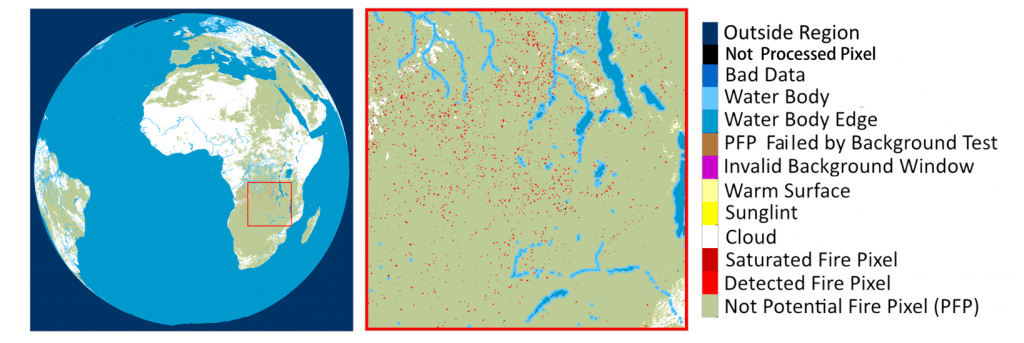
\includegraphics[width=1\linewidth]{images/Meteosat_FRP_pixels.png}
    \caption{\footnotesize{Example Meteosat SEVIRI FRP-PIXEL Product example, derived from SEVIRI imagery collected at 13:00 UTC on 5\textit{th}\textit{ July 2015}. Meteosat is one of the geostationary sensors from FIRMS.\cite{_access_kings_wildfire}}}
    \label{fig:Meteosat_FRP_pixels}
\end{figure}
\subsubsection{Confidence of Fire Event Detection}

To minimize false positives in the validation dataset, we enforce strict classification boundaries: a minimum Fire Radiative Power of $FRP_{min} = 50\,\mathrm{MW}$ and a \textbf{Confidence Level of 100\%} \inlineReq{R27}. In the FIRMS algorithm, confidence is a metric from detection data (e.g., anomaly strength, sun glint potential). Choosing "High Confidence" (100\%) pixels filters the dataset to events with saturated readings or strong anomalies (>15K), removing sun glint, weak signals, and ambiguous detections.s detections\cite{earthsciencedatasystems_viirs_2024}.


\subsection{Key Multi-spectral Bands for Broad Fire Analysis}
\label{312-key-spectral-bands-for-fire-analysis}

To satisfy mission requirements for fire resilience \reqRef{R1}, ignition anticipation \reqRef{R2}, and all-weather capability \reqRef{R5}, a comprehensive mission would  need a diverse multispectral payload:

\begin{itemize}
    \item \textbf{Visible (VIS):} Essential for tracking smoke plume dynamics, distinguishing clouds from smoke, and providing intuitive geographic context for ground teams.
    \item \textbf{Near-Infrared (NIR):} Key for assessing vegetation health (fuel load estimation) and mapping post-fire burn scars.
    \item \textbf{SWIR:} Identifies high-temperature anomalies and moisture contrast (discriminating hot ground from warm smoke).
    \item \textbf{MWIR \& LWIR:} The primary bands for active heat detection, temperature retrieval, and FRP calculation.
    \item \textbf{SAR:} Enables all-weather biomass mapping and fire line detection through thick smoke and clouds (structural change detection).
\end{itemize}

However, detailed instrument optimization is outside the scope of this geometric analysis. We leave detailed instrument design tradeoffs for future research. For this study, we assume standard detection capabilities based on the FRP principles described  \inlineReq{R28}. This assumption is robust for the core study domain, as most fire seasons occur during hot, cloud-free periods.

It is important to recognize that this approach relies on optical visibility. Specific operational scenarios, such as mega-fire events with high smoke density, tropical cloud cover, or coastal regions where diurnal fog obscures morning hotspots (e.g., the Portuguese coast), would require the SAR or multispectral capabilities mentioned to maintain continuity, early detection, and effective fire combat. SAR is also a prominent new technology for combating fires in tropical forests, which are very often obscured by dense clouds. These instrumentation trade-offs are reserved for future research; the current focus remains on the satellite network geometry, the sensors' field of view, and the spacecraft system's coverage.

%%%%%%%draft
\section{Sensor Observation Constraints}
\label{sec:sensor_observation_constraints}

The temporal resolution performance of a constellation is driven by the revisit time $t_{rev \to P_j}$ to a target $P_j$. The revisit frequency depends on the trade-off between the network's satellite density and the duration and quality of each pass, which are governed by the individual sensor's geometric and optical limits.

The detailing constellation observation formalism connected with orbital dynamics is discussed in the Methodology (Chapter \ref{sec:Constellation_observation_form}). Before this details, to limit the scope of work, we must first define the physical limits of the atmosphere which will lead to observation constraints. A valid detection event is not merely a line-of-sight problem; it requires the signal quality of the intersection of two distinct geometric volumes: the \textbf{Ground Access Window} (the ground target's view of the sky) and the \textbf{Space Access Window} (the satellite's view of the ground), as shown in Fig \ref{fig:access_nominal_and_limit}.

\subsection{Physical Limit: Atmospheric Attenuation}
\label{subsec:atmospheric_limit}
As discussed in the Radiance Chapter, the infrared signal is modulated by the atmospheric transmittance $\tau_\lambda$ (Eq. \ref{eq:tranmitance_atm}). Factors such as clouds, smoke aerosols, and water vapor significantly attenuate the signal.

Observations at low elevation angles $\varepsilon$ (near the horizon) traverse a much thicker atmospheric layer compared to the Zenith path, drastically degrading the Signal-to-Noise Ratio (SNR). The path length through the atmosphere scales with $\approx 1/\sin(\varepsilon)$. 

To mitigate these effects without performing complex real-time radiative transfer modelling, we impose a strict geometric constraint. We define the operational limits: the \textbf{Minimum Elevation Angle} $\varepsilon_{min} = 15^\circ$, \inlineReq{R29}, and \textbf{Maximium Athmospheric grazing angle} $\theta{\text{atm max}}=65^\circ$, \inlineReq{R30}. 

This threshold acts as a proxy for signal quality, filtering out observations where transmittance is likely to be dominated by scattering and absorption.

\subsection{Geometric Access Windows}
Based on the physical limit defined above, we construct two geometric volumes that define the valid observation space, as illustrated in Fig. \ref{fig:access_nominal_and_limit}.

\begin{figure}[H]
    \centering
    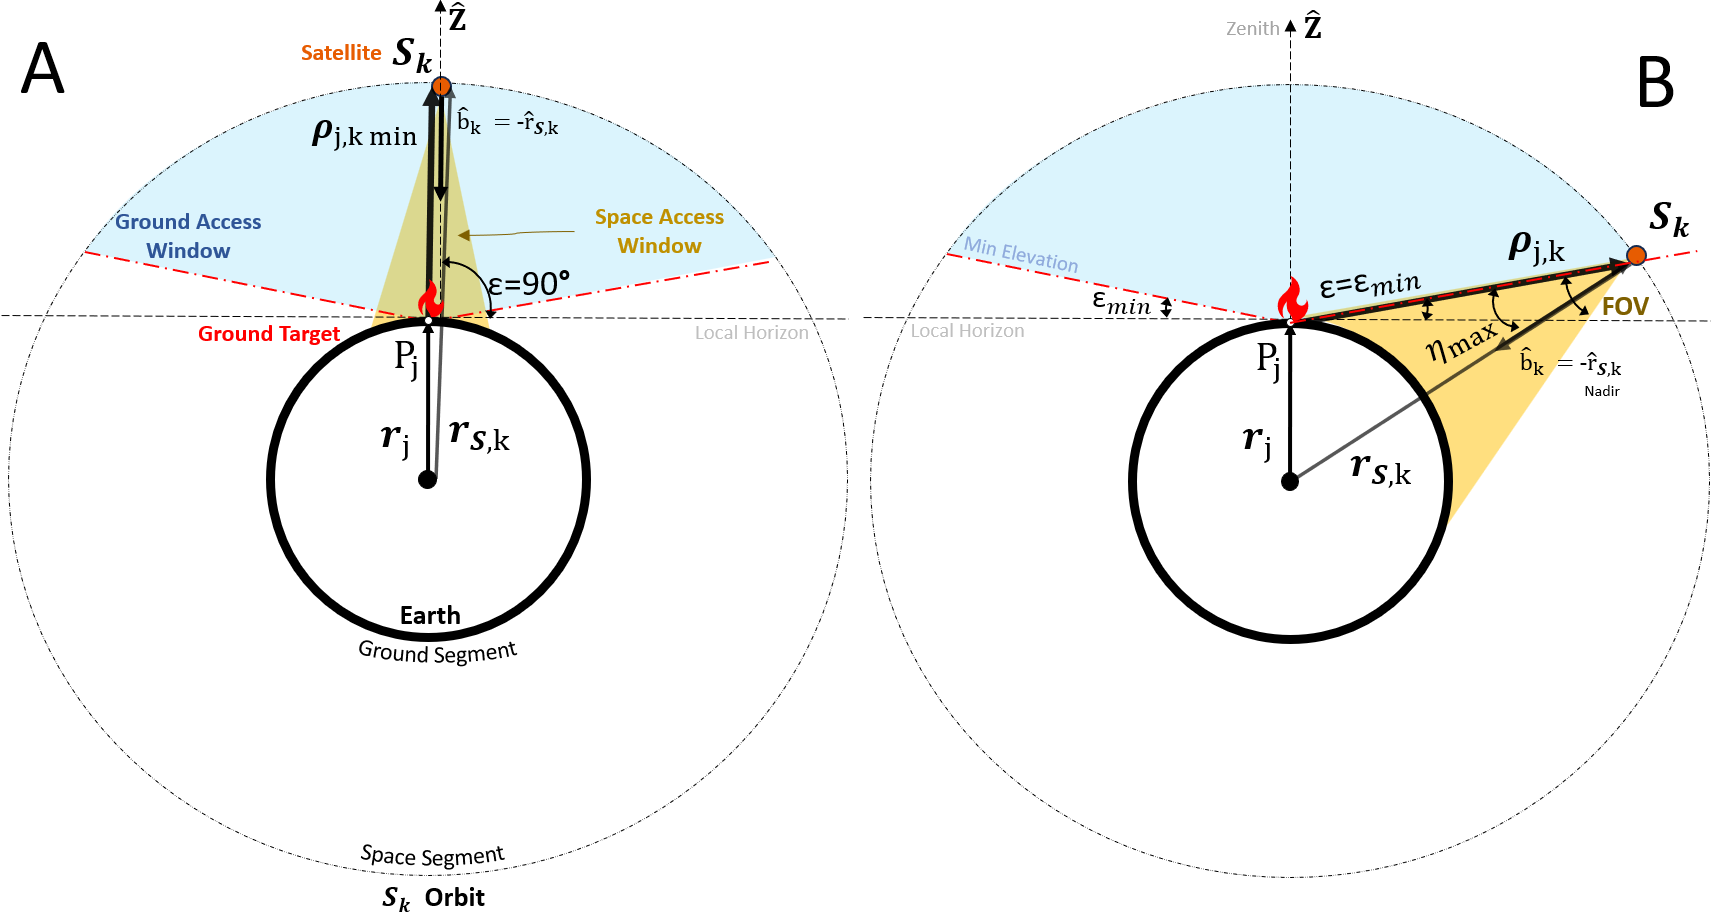
\includegraphics[width=1\linewidth]{images/access_nominal_and_limit.png}
    \caption{\footnotesize{Geometric definition of the Observation Constraints. The valid detection volume is formed by the intersection of the Ground Access Window (Blue) and the Space Access Window (Yellow). A) Highlights the Nominal Zenith case (best quality) where ground resolution GSD is calculated. B) Visibility limit configuratrion, edge of the coverage where Ground \& Space Access windows meet ($\epsilon_{min}$ and $\eta_{max}$).}}
    \label{fig:access_nominal_and_limit}
\end{figure}

\subsection{Ground Access Window ($\mathcal{W}_{ground}$)}
The Ground Access Window $\mathcal{W}_{ground,j}$ represents the volume of the local sky physically visible and useful to the target point $P_j$. While a target theoretically has a $180^{\circ}$ view of the sky (from horizon to horizon), practical observation is limited by terrain geometric masking and atmospheric attenuation.

We define the constraint using the \textbf{Elevation Angle $\varepsilon$}, measured from the local horizon to the satellite. To ensure valid data retrieval, the satellite must be above a minimum elevation threshold:
\begin{equation}
    \mathcal{W}_{ground,j} = \{ \text{Visible} \mid \varepsilon \geq \varepsilon_{min} \}
\end{equation}
For this mission analysis, as discussed, we set the requirement to $\varepsilon_{min} = 15^{\circ}$. Below this angle, the path length through the atmosphere increases drastically, degrading the signal-to-noise ratio and geometric accuracy.

\subsection{Space Access Window ($\mathcal{W}_{space}$)}
The Space Access Window represents the conical volume observable by the spacecraft $S_k$. This volume encloses all potential instrument architectures (e.g., push-broom scanners, matrix cameras) and is defined relative to the satellite's Sensor Boresight Vector $\hat{\mathbf{b}}_k$, which nominally points toward the geodetic Nadir.

We define the constraint using the \textbf{Off-Nadir Angle $\eta$}, measured from the boresight vector $\hat{\mathbf{b}}_k$ to the the Relative Position Vector $\vec{\rho}_{j,k}$ between ground target $P_j$ and the satellite $S_k$. The limit is determined by the maximum reachable angle of the spacecraft optical system:
\begin{equation}
    \mathcal{W}_{space} = \{ \text{Visible} \mid \eta \leq \eta_{max} \}
\end{equation}
For a standard Earth-observation missions (LEO-MEO), achieving the good quality optical signal typically demands a maximum off-nadir view of $\eta_{max} = \theta{\text{atm max}} \approx 65^{\circ}$, \inlineReq{R31}. This cone defines the max Full Field of View for the satellites, \inlineReq{R32}.
\begin{equation}
    FOV = 2  \eta_{max} = 130^\circ; 
\end{equation}
\subsection{The Visibility Condition}
Consequently, a fire event at $P_j$ is only detected when the satellite enters the intersection of these two windows as shown in Fig \ref{fig:access_nominal_and_limit}-B. The geometric requirement for observation is the simultaneous satisfaction of both access windows angular constraints\inlineReq{R33}:

\begin{equation}
    \text{Observation Link} \ \mathcal{L}_{j,k} \iff Visible
    \begin{cases} 
        \varepsilon \geq 15^{\circ} & \text{(Ground access: clear sky horizon)} \\
        \eta \leq 65^{\circ} & \text{(Space access : sensor athmospheic gazing limit)}
    \end{cases}
\end{equation}

\subsection{Optical Quality: Ground Sample Distance (GSD)}
\label{optical-quality}
The spatial resolution of the detected fire is governed by the \textbf{Ground Sample Distance (GSD)}. For this constellation design analysis we have the spacecraft at the nadir configuration as shown in Fig \ref{fig:access_nominal_and_limit}-A. On this observation setting, we utilize the first-order paraxial approximation calculated at nadir, \inlineReq{R34}. The GSD is deffined in function of the satellite altitude $h(t) = \|  \vec{\rho}_{j,k}  \|$:
\begin{equation}
    \text{GSD}(t) \approx \frac{p \cdot h[n]}{f}
    \label{eq:gsd}
\end{equation}
where $p$ is the detector pixel pitch and $f$ is the effective focal length. Athmospheric effects is not taking in consideration. 

\paragraph{Simulation Parameters:}
For the specific instrument modeled in this thesis, we assume the following optical characteristics:
\begin{itemize}
    \item Pixel Pitch: $p = 12um $ 
    \item Focal Length: $f = 600mm$ 
\end{itemize}

\paragraph{High-Fidelity Simulation Requirements.}
It is important to note that this linear approximation represents the "best-case" scenario. It does not account for off-nadir distortion where GSD degrades, optical aberrations, or motion smear. A rigorous validation of these parameters requires end-to-end optical simulation using Fourier optics tools (e.g., \textbf{Zemax OpticStudio}) and ruggedized geolocation libraries (e.g., \textbf{Rugged}), \cite{segl_s2etes_2015}, \cite{alici_image_2019}, \cite{_rugged_}. 

\section{Daily Fire-Behavior Temporal Observation Requirements}
\label{sec:_fire_daily_temporal_requirements}

Fires exhibit diurnal behavior driven by the daily evolution of atmospheric conditions, solar irradiance, temperature, relative humidity, and wind speed. This cycle is characterized by the temporal profiles of \textbf{Fire Radiative Power (FRP)}. Different types of sensors may be needed to investigate this variable temporal response, but they are out of scope, as discussed in section \ref{312-key-spectral-bands-for-fire-analysis}. However, we still need a "peak-fire hour" to synchronize the constellation at the $t_{\text{peak fire ref day}} = \text{ August 18th}$ at Coimbra, described in \reqRef{R16}.

Generally, the daily fire cycle has a spectrum of radiance that follows a loop relative to solar irradiation:
\begin{enumerate}
    \item \textbf{Smoldering Phase (Night/Early Morning, $\sim$00:00--09:00):} Higher humidity and lower temperatures suppress combustion, often reducing fires to a smoldering state (low FRP).
    \item \textbf{Growth Phase (Late Morning, $\sim$09:00--13:00):} Solar heating breaks the nocturnal pattern, lowering humidity and increasing wind mixing, causing a rapid ramp-up in FRP.
    \item \textbf{Peak Intensity (Afternoon, $\sim$13:00--18:00):} The coincidence of maximum temperature and wind speeds drives the fire to its maximum radiative output.
    \item \textbf{Decay Phase (Evening, $\sim$18:00--23:00):} As solar forcing vanishes, the boundary layer stabilizes, and intensity gradually declines.
\end{enumerate}

\subsection{Operational Windows for Portugal}
In Portugal, correlating peak fire activity with the diurnal temperature maximum (typically 13:00--15:00) can be misleading. The region is strongly influenced by strong Atlantic oceanic winds (e.g., the Nortada), which often intensify in the afternoon, decoupling peak fire intensity from peak solar irradiance. While a rigorous historical analysis of past fire events is necessary to precisely calibrate sensor timing for specific micro-climates, this study prioritizes aligning the constellation's orbit to intercept the estimated \textbf{maximum FRP peak at approximately 15:00 Local Time at Coimbra}, \inlineReq{R35}. 

\begin{equation}
    t_{\text{peak fire ref hour}} = \text{ 15:00 Local Time @ Coimbra }
    \label{eq:peak_fire_ref_hour}
\end{equation}


\section{Requirements of Fire Observation
Summary}\label{33---requirements-of-fire-observation-summary}

This section consolidates the fire remote-sensing constraints derived in the preceding sections into traceable, design-level requirements. These requirements establish the radiometric detection standard, the geometric observation boundaries, the optical resolution model, and the temporal synchronization reference for the constellation simulation. The requirements are organized into four categories: Fire Characterization, Sensor Observation Geometry, Optical Quality, and Temporal Observation.


Detailed requirements derived in this chapter (R26--R35), including Fire Characterization, Sensor Observation Geometry, Optical Quality, and Temporal Observation, are provided in Appendix~\ref{sec:app_req_ch3}.

% --- CHAPTER 4: State of the Art in Fire Remote Sensing ---
% \chapter{State of the Art in Spaceborne Wildfire
Monitoring: History and Current
Gaps}\label{chapter-4-state-of-the-art-in-spaceborne-wildfire-monitoring--history-and-current-gaps}

\begin{quote}
\textbf{Writing Guide \& Methodological Focus:}

\begin{itemize}
\item
  \textbf{Objective:} Show how wildfire EO evolved, what systems exist
  today, and where they still miss or mission requirements.
\item
  \textbf{Method:} Tell the \textbf{history by epochs} → compile a
  \textbf{systems comparison table} → add a brief \textbf{modality
  overview} → close with a \textbf{gap matrix} vs requirements.
\item
  \textbf{Caution:} Tell a story of progress and remaining challenges,
  don\textquotesingle t just list missions. Describe capabilities and
  limits; do \textbf{not} design the constellation here.
\item
  \textbf{Checkpoint:} Does this chapter successfully demonstrate that,
  despite decades of progress, a specific and important capability gap
  still exists? Can a reader point to concrete shortfalls this work
  design must close (tempospatial resolution(GSD, latency), observation
  in core bands, all-weather reliability)?
\end{itemize}
\end{quote}

\section{Historical evolution}\label{41-historical-evolution}

Four short phases---Foundations (1970-1999), Global Monitoring
(1999--2012), Multi-sensor convergence (2013--2019), NewSpace \& rapid
analytics (2020--present)---ending with ``lessons learned.''

\subsection{The Foundational Era (1970s --
1990s)}\label{411-the-foundational-era-1970s----1990s}

\begin{itemize}
\item
  Cover the first thermal detections and post-fire mapping with Landsat.
\end{itemize}

\subsection{The Era of Global Monitoring (2000 --
2015)}\label{412-the-era-of-global-monitoring-2000----2015}

\begin{itemize}
\item
  Discuss MODIS, the impact of the open-data policy, and the rise of
  commercial VHR.
\item
  Introduce the Copernicus Sentinel missions.
\end{itemize}

\subsection{The NewSpace Revolution (2015 --
Present)}\label{413-the-newspace-revolution-2015----present}

\begin{itemize}
\item
  Cover VIIRS, commercial constellations (Planet, ICEYE), and
  purpose-built fire constellations (FireBIRD, OroraTech, FireSat).
\end{itemize}

\section{Comparative Synthesis EO Wildfire
systems}\label{42-comparative-synthesis-eo-wildfire-systems}

One table with columns: \textbf{Name \textbar{} First launch \textbar{}
Operational \textbar{} Application \textbar{} Region of interest
\textbar{} Orbit \textbar{} \# sats \textbar{} Spatial res \textbar{}
Temporal res \textbar{} VNIR \textbar{} SWIR \textbar{} MWIR \textbar{}
LWIR \textbar{} SAR \textbar{} FOV (deg) \textbar{} Swath @ nadir (km)
\textbar{} Max off-nadir (deg) \textbar{} Tip-and-cue (Y/N) \textbar{}
Slew/retask (typ.) \textbar{} Tasking autonomy (Y/N)};

conclude with the single-sentence takeaway that there is \textbf{no
regional, all-weather constellation} meeting \textless30 min sub-hour
cadence + \textless10m meter-class thermal over Portugal's daily fire
cycle.

\section{Modality overview (capabilities \&
limits)}\label{43-modality-overview-capabilities--limits}

In one paragraph each, summarize \textbf{GEO}, \textbf{SSO},
\textbf{RGTO}, \textbf{polar medium-res thermal}, \textbf{high-res
optical/thermal}, \textbf{SAR/microwave}---what each does well for fires
and where each misses for the regional Portuguese case.§2.6 (cadence,
GSD, weather/angle robustness, latency). In the methodology, a detailed
trade-off of these types of orbit will be done. This subchapter shall be
used to filter from the table other requirements for our modality

\section{Regional fit: Portugal vs seasonal
windows.}\label{44-regional-fit-portugal-vs-seasonal-windows}

How current systems actually cover Portugal's \textbf{seasonal} and
\textbf{core local-time} bands; note where QC (cloud/smoke/angle)
removes scenes.

\section{Latency, access, and tasking
realities.}\label{46-latency-access-and-tasking-realities}

Typical acquisition→alert latency ranges, downlink/ground constraints,
and practical tasking/retasking windows during peak fire hours. Connect
to the Portuguese architecture of wildfire management.

\section{Coverage geometry, swath, agility \& tip-and-cue
capability}\label{47-coverage-geometry-swath-agility--tip-and-cue-capability}

Show that wide \textbf{FOV} without \textbf{pointing agility} reduces
\textbf{effective swath} and increases complexity in optics, difficulty
the coverage in core fire daily cycle windows, and note the emerging
constellation with \textbf{two-layer layers tip-and-cue} (wide FOV
``tipper'' + agile narrow FOV ``cuer'') as a way to tile Portugal's
seasonal bands more efficiently decreasing hardware constraints.
\textbf{Output:} A requirement seed: \emph{support tip-and-cue within
core local-time bands, respecting maximum allowed view-zenith angle (θ)
and ≤{[}TBD{]} retask latency}.

\section{Synthesis, Mission Requirements Vs EO Wildfire
Capability-Gap
Matrix}\label{48--synthesis-mission-requirements-vs-eo-wildfire-capability-gap-matrix}

One-page matrix aligning \textbf{mission requirements} (AOI/ROIs,
seasonal \& daily fire windows, max revisit, GSD, θ-cap, latency,
transferability) against each EO Wildfire mission/modality, highlighting
\textbf{where gaps remain} and which are only partially covered. Check
if new requirements are needed.



% --- Chapter 5: Research Hypotheses, Questions \& Pre-Phase A Closure
% \chapter{Research Hypotheses, Questions \& Pre-Phase A
Closure}\label{chapter-5-research-hypotheses-questions--pre-phase-a-closure}

\begin{quote}
\textbf{Writing Guide \& Methodological Focus:}

\begin{itemize}
\item
  \textbf{Objective:} To formally state the central hypothesis and the
  specific, testable questions that the research will answer. State the
  science that will be tested, then close \textbf{Pre-Phase A} with a
  light, systems-engineering frame that shows the methods that will be
  used.
\item
  \textbf{Method:} Short synthesis → one-line hypothesis → concise
  research questions → hint-level Pre-Phase-A closure
  (needs/goals/objectives → constraints → success criteria) → note the
  concept options to be tested.
\item
  \textbf{Caution:} This chapter should be short and direct. It is the
  pivot point between the background and this thesis's original work.
  Keep it brief and directional; traceable requirements IDs, success
  criteria and tables here.
\item
  \textbf{Checkpoint:} Is the methodology described in Part II directly
  answerable to the research questions? After this chapter, the reader
  knows what will be tested* and \emph{the frame it must satisfy}.
\end{itemize}
\end{quote}

\section{Synthesis of the
Problem}\label{51-synthesis-of-the-problem}

Update the Chapter 1 Problem Statement with condensed information from
Chapters 2--4 into a single Problem Statement paragraph

\subsection{Primary Research
Hypothesis}\label{52-primary-research-hypothesis}

Assert that a \textbf{Portugal-tuned, tip-and-cue LEO all-weather
wildfire constellation} can meet the need more effectively than
conventional single-layer designs.

\section{Key Research
Questions}\label{53-key-research-questions}

List of questions; cadence vs orbit geometry; constellation sizing/plane
spacing; single vs two-layer (tipper+cuer); angle/quality policy impact;
robustness under typical cloud/smoke; latency pathway; transferability
to secondary ROIs.

\section{\texorpdfstring{Pre-Phase-A Closure
}{Pre-Phase-A Closure }}\label{54-pre-phase-a-closure}

Clarify that we are using the Nasa System Engineering approach to
develop the concept of this mission. Explain the evolution of this
structure. Add the system engineering thesis structure.

\subsection{Needs, goals,
objectives}\label{541-needs-goals-objectives}

Freeze a brief structure condensing all mission requirements build into
here

\subsection{Constraints}\label{542-constraints}

Note the boundary conditions you will work

\subsection{Success criteria}\label{543-success-criteria}

Table with success for each requirement

\subsection{Mission Concept
Options}\label{544-mission-concept-options}

From the background development, suggest concepts to be verified in the
development of Part II: Methodology and Mission Design, such as
constellation type (single vs. two-layer), orbit class, plane/phasing
patterns, and high-level sensor families/limits.


% --- Part II: METHODOLOGY AND MISSION DESIGN ---
% ----------------------------------------
\part{\texorpdfstring{\textbf{METHODOLOGY AND MISSION
DESIGN}}{PART II: METHODOLOGY AND MISSION DESIGN}}
\label{part-ii-methodology-and-mission-design}

% --- Chapter 6 :Phase A, Mission Design and
% Methodology 
% \chapter{Phase A, Mission Design and
% Methodology}\label{chapter-6-phase-a-mission-design-and-methodology}

% Observation, this chapter needs to be rethought.

% \begin{quote}
% \textbf{Writing Guide \& Methodological Focus:}

% \begin{itemize}
% \item
%   \textbf{Objective:} To make the transition from Pre-Phase A, defining
%   the "problem space" to the Phase A "solution space" for design,
%   following a structured process.
% \item
%   \textbf{Method:} Blend a systems engineering and framework with a
%   clear description of the simulation setup.
% \item
%   \textbf{Checkpoint:} Is it perfectly clear what the thesis is trying
%   to achieve (concepts - requirements) and how the orbital mission
%   simulation is setup to find the best architecture?
% \end{itemize}
% \end{quote}

% \section{A Systems Engineering
% Approach}\label{61-a-systems-engineering-approach}

% \begin{itemize}
% \item
%   State that you will follow a structured design process analogous to
%   standard space mission design phases (e.g., based on NASA/ECSS
%   standards).
% \item
%   Outline the flow: Mission Objectives -\textgreater{} System
%   Requirements -\textgreater{} Candidate Concepts -\textgreater{} Trade
%   Space Analysis -\textgreater{} Baseline Design.
% \end{itemize}

% \section{Simulation and Analysis
% Approach}\label{62-simulation-and-analysis-approach}

% \begin{itemize}
% \item
%   \textbf{6.3.1 Trade Space Definition:}
% \item
%   \textbf{6.3.2 Simulation Environment and Tools:}
% \item
%   \textbf{6.3.3 Analysis Method:}
% \end{itemize}


% --- Chapter 7: Fundamentals of Satellite Constellation
\chapter{Fundamentals of Satellite Constellation
Design}\label{chapter-7-fundamentals-of-satellite-constellation-design}

This chapter establishes the theoretical foundation required to understand the constellation design and analysis that follow. It opens with the observation formalism --- defining how a satellite constellation covers a ground domain and what conditions must hold for a target to be visible to a sensor. It then develops the orbital mechanics principles --- classical orbital elements, the dominant gravitational perturbation, and the resonance condition --- that underpin the Repeating Ground Track Orbit selected for this mission.

\section{Constellation Observation Formalism Introduction}
\label{sec:Constellation_observation_form}
%Improve intro reflection full section
We have previously defined the study domains $\mathcal{D}$ on the Earth's surface. However, for a fire event to be detected, it must fall within the observable coverage domain of the satellite constellation $\mathcal{D_{Cover}}$.  

\subsection{Constellation Definition and State Space}
The satellite constellation is defined as a set of $N$ discrete spacecraft nodes:
\begin{equation}
    \mathcal{C}_{sat} = \{ S_k \}_{k=1}^{N}
\end{equation}
Each satellite $S_k$ is uniquely defined by its \textbf{Orbital State Element} $\vec{A}_k$:
\begin{equation}
    S_{k} \equiv \vec{A}_k
\end{equation}
This vector encapsulates the state-space parameters required to propagate the spacecraft's trajectory. It is composed of the six classical Keplerian orbital elements and a reference epoch, as formally defined in Sec.~\ref{sec:classical_orbital_elements}.


\subsection{Single-Satellite Sensor Visibilty Toward a Ground Target}
This section defines the geometric boundaries and optical constraints that govern the visibility link between a ground target and a spacecraft sensor. The revisit time $t_{rev \to P_j}$ of a satellite $\mathcal{S}_{k}$ over a ground point target $P_{j}$ is fundamentally limited by the geometric constraints of the spacecraft sensor relative to the ground location. To quantify these constraints, such as whether a target is above the local horizon or within the sensor's field of view, we must define a coordinate frame system centered on the observer's location at the ellipsoid surface $\mathcal{E_\oplus}$. The detailed definition of such a local frame, the satellite and ground trajectory, is done in the section. 

\paragraph{Satellite Position Trajectory:}
To analyze the geometry of the sensor-to-target mapping, we first define the trajectories of the spacecraft and the ground targets as time-dependent mappings on the inertial manifold $\mathcal{M}$, as defined in eq. \ref{eq:manifold}. Then, we define the $k$-th satellite $S_k$ as a point mass moving in the inertial frame. Its orbital position with respect to Earth's center of mass $O_{\oplus}$ is defined by the position vector function $\vec{r}_{s,k}$:
\begin{equation}
    \vec{r}_{s,k} : \mathcal{T}_{sim} \to \mathcal{M}, \quad t \mapsto \overrightarrow{r_{s,k}}(t) = \overrightarrow{O_{\oplus}S_{k}}(t)
\end{equation}
\paragraph{Ground Target Trajectory:}
The ground target $P_j$ is fixed to the surface of the WGS84 Reference Ellipsoid $\mathcal{E}_\oplus$. However, due to the Earth's rotation, $P_j$ describes a trajectory in the inertial frame $\mathcal{F}_{J2000}$. We define this motion as the vector function $\vec{r}_j$:
\begin{equation}
    \vec{r}_{j} : \mathcal{T}_{sim} \to \mathcal{M}, \quad t \mapsto \overrightarrow{r_j}(t) = \overrightarrow{O_{\oplus}P_{j}}(t)
\end{equation}
\subsubsection{Topocentric Horizon Coordinate System (SEZ)}
The Topocentric Horizon Coordinate System $\mathcal{F}_{SEZ}$ is the standard frame for defining "look angles" between a ground site and a satellite. We adopt the deffitintion of $\mathcal{F}_{SEZ}$ as done by Vallado\cite{mcclain2001fundamentals}. This frame is also known as $\mathcal{F}_{AltAz}$ because it measures the altitude, also known as elevation $\epsilon$,  and azimuth $\beta$ as shown in Fig. \ref{fig:sez_frame}. This system rotates with the site location $P_{k}$.

\begin{figure}
    \centering
    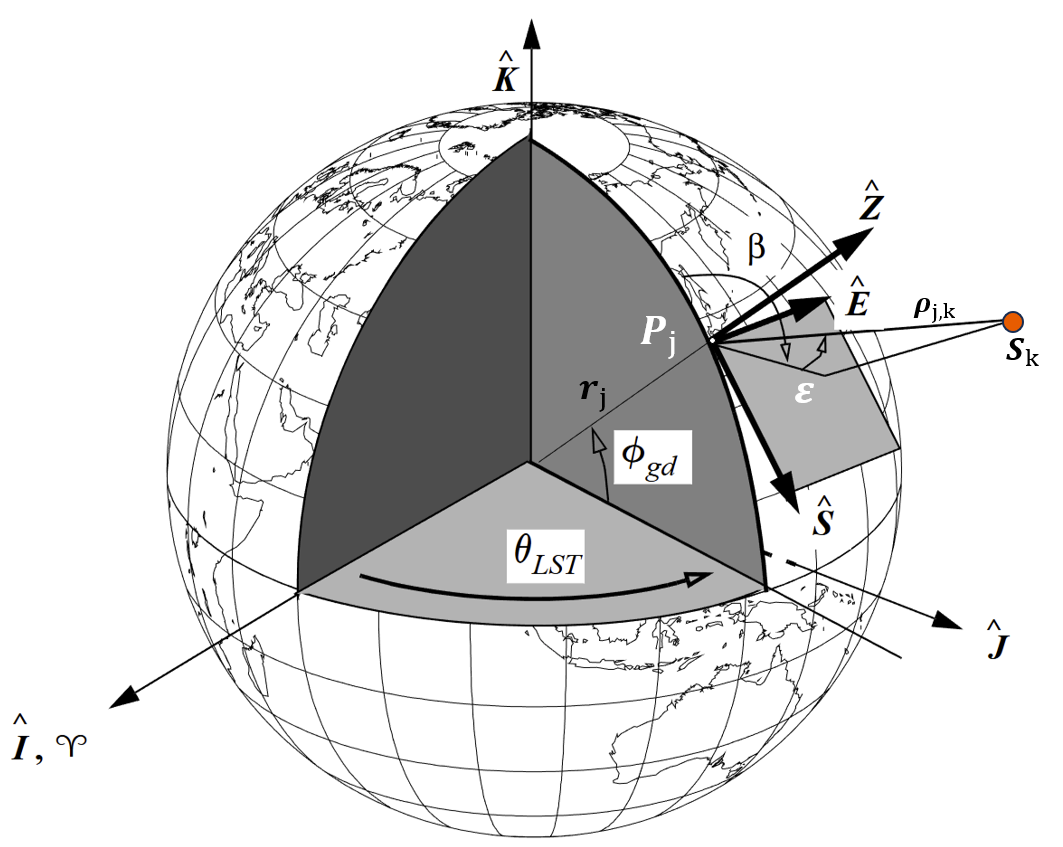
\includegraphics[width=0.5\linewidth]{images/Topocentric_Horizon_Coordinate_System_SEZ.png}
    \caption{\footnotesize{The Topocentric Horizon Coordinate System  $\mathcal{F}_{SEZ}$, "South, East, Zenith frame", or $\mathcal{F}_{AltAz}$. The frame originates at the site location $P_k$ on the Earth's elipsoid $\mathcal{E_\oplus}$. The fundamental plane is the local horizon. The $\hat{S}$ axis points South, the $\hat{E}$ axis points East, and the $\hat{Z}$ axis (Zenith) points radially outward along the local vertical. $\mathcal{F}_{SEZ}$ defines the observation geometry: Azimuth $\beta$ measured clockwise from North, and Elevation $\epsilon$ measured from the horizon plane up to the vector $\rho_{j,k}$ measuring the relative distance between satellite $S_k$ and the ground target $P_j$ .}}
    \label{fig:sez_frame}
\end{figure}
This planetary mobile local frame is is defined by the orthonormal basis $\mathcal{B}_{SEZ} = \{ \hat{\mathbf{s}}, \hat{\mathbf{e}}, \hat{\mathbf{z}} \}$ centered at the target $P_j$, $\mathcal{F}_{SEZ} \equiv  \{ P_{j};\hat{\mathbf{s}}, \hat{\mathbf{e}}, \hat{\mathbf{z}} \}$.  The unit vectors are defined as: $\hat{\boldsymbol{s}}$ (South) along the local meridian, $\hat{\boldsymbol{e}}$ (East) along the local parallel, and $\hat{\boldsymbol{z}}$ (Zenith) along the local vertical

\paragraph{Line-of-Sight (LOS) Vector:}
The relative geometry is governed by the vector connecting the ground target $P_j$ to the satellite $S_k$. We construct this \textbf{Line-of-Sight Vector} $\vec{\rho}_{j,k}$ via the vector subtraction map:
\begin{equation}
    \vec{\rho}_{j,k} : \mathcal{T}_{sim} \to \mathcal{M}, \quad t \mapsto \overrightarrow{\rho_{j,k}}(t) = \overrightarrow{P_{j}S_{k}}(t) = \overrightarrow{r_{s,k}}(t) - \overrightarrow{r_{j}}(t)
\end{equation}

This vector is projected onto the local basis $\mathcal{B}_{SEZ}$ as:
\begin{equation}
    \vec{\rho}_{j,k} = \rho_s \hat{\mathbf{s}} + \rho_e \hat{\mathbf{e}} + \rho_z \hat{\mathbf{z}}
\end{equation}
%%
\paragraph{Relative Position Vector ($\vec{\rho}_{j,k}$):}
The geometry is commanded by the relative displacement between the ground target $P_j$ and the satellite $S_k$. We define the \textbf{Relative Position Vector}  $\vec{\rho}_{j,k}$ via the vector subtraction map:
\begin{equation}
    \vec{\rho}_{j,k} : \mathcal{T}_{sim} \to \mathcal{M}, \quad t \mapsto \vec{\rho}_{j,k}(t) = \overrightarrow{P_{j}S_{k}}(t) = \overrightarrow{r_{s,k}}(t) - \overrightarrow{r_{j}}(t)
\end{equation}
This vector represents the physical distance and direction from the target to the satellite, independent of where the satellite is facing. It is projected onto the local basis $\mathcal{B}_{SEZ}$ as:
\begin{equation}
    \vec{\rho}_{j,k} = \rho_s \hat{\mathbf{s}} + \rho_e \hat{\mathbf{e}} + \rho_z \hat{\mathbf{z}}
\end{equation}
\paragraph{Sensor Boresight Vector ($\hat{\mathbf{b}}_k$):}
Distinct from the relative position, the satellite $S_k$ observation capability depends on its attitude and sensor direction. We define the Sensor Boresight Vector (or Line-of-Sight direction) as the unit vector $\mathbf{b}_{k}$  representing the optical axis of the instrument in the inertial frame:
\begin{equation}
    \hat{\mathbf{b}}_{k} : \mathcal{T}_{sim} \to \mathcal{M}, \quad t \mapsto \hat{\mathbf{b}}_{k}(t) = \mathbf{A}(t) \cdot \hat{\mathbf{b}}_{body}
\end{equation}
where, for $S_k$, $\mathbf{A}(t)$ is the attitude rotation matrix and $\hat{\mathbf{b}}_{body}$ is the fixed sensor axis in the satellite body frame.

\paragraph{Look Angles Definition:}
From these components, we define the look angles as the mapping $\Lambda_{look}: \mathbb{R}^3 \to \mathbb{R}^2$:

\begin{enumerate}
    \item \textbf{Elevation ($\varepsilon$):} The angular height above the local horizon plane. It is derived from the angle between the local zenith $\hat{\mathbf{z}}$ (aligned with $\hat{\boldsymbol{r}}_{j}$ for a spherical approximation) and the relative vector:    \begin{equation}
        \epsilon_{k,j} = \sin^{-1}\left( \frac{\vec{\rho}_{j,k} \cdot \hat{\mathbf{z}}}{\| \vec{\rho}_{j,k} \|} \right), \quad \varepsilon \in \left[ -\frac{\pi}{2}, \frac{\pi}{2} \right]
    \end{equation}
    A positive elevation ($\varepsilon > 0$) indicates that the satellite is above the local geometric horizon and may be able to observe $P_j$, depending on the spacecraft's sensor field of view, line-of-sight orientation, and atmospheric transmission. 
    \item \textbf{Azimuth ($\beta$):} The orientation angle measured clockwise from North ($-\hat{\mathbf{s}}$) to the projection of the satellite vector on the horizon plane.
\begin{equation}
        \beta_{k,j} = \operatorname{atan2}(\rho_e, -\rho_s), \quad \beta \in [0, 2\pi)
    \end{equation}
    where $\operatorname{atan2}(y, x)$ is the multi-valued inverse tangent function used to resolve quadrant ambiguity.
\end{enumerate}

\section{Observational Access}
\label{sec:observational_access}
To formally characterize the observation geometry, we adapt the constellation observation visibility framework established by Lee et al. \cite{lee_satellite_2020}. We introduced the sensor constraints as a condition for visibility.
For a valid observation to occur, the geometric link must satisfy constraints from two distinct reference frames: the target's local horizon (Ground Segment) and the satellite's instrument orientation (Space Segment). As illustrated in Figure \ref{fig:access_window_configs}, visibility is only achieved when the Line-of-Sight (LOS) vector falls within the intersection of these two independent access volumes.

\begin{figure}
    \centering
    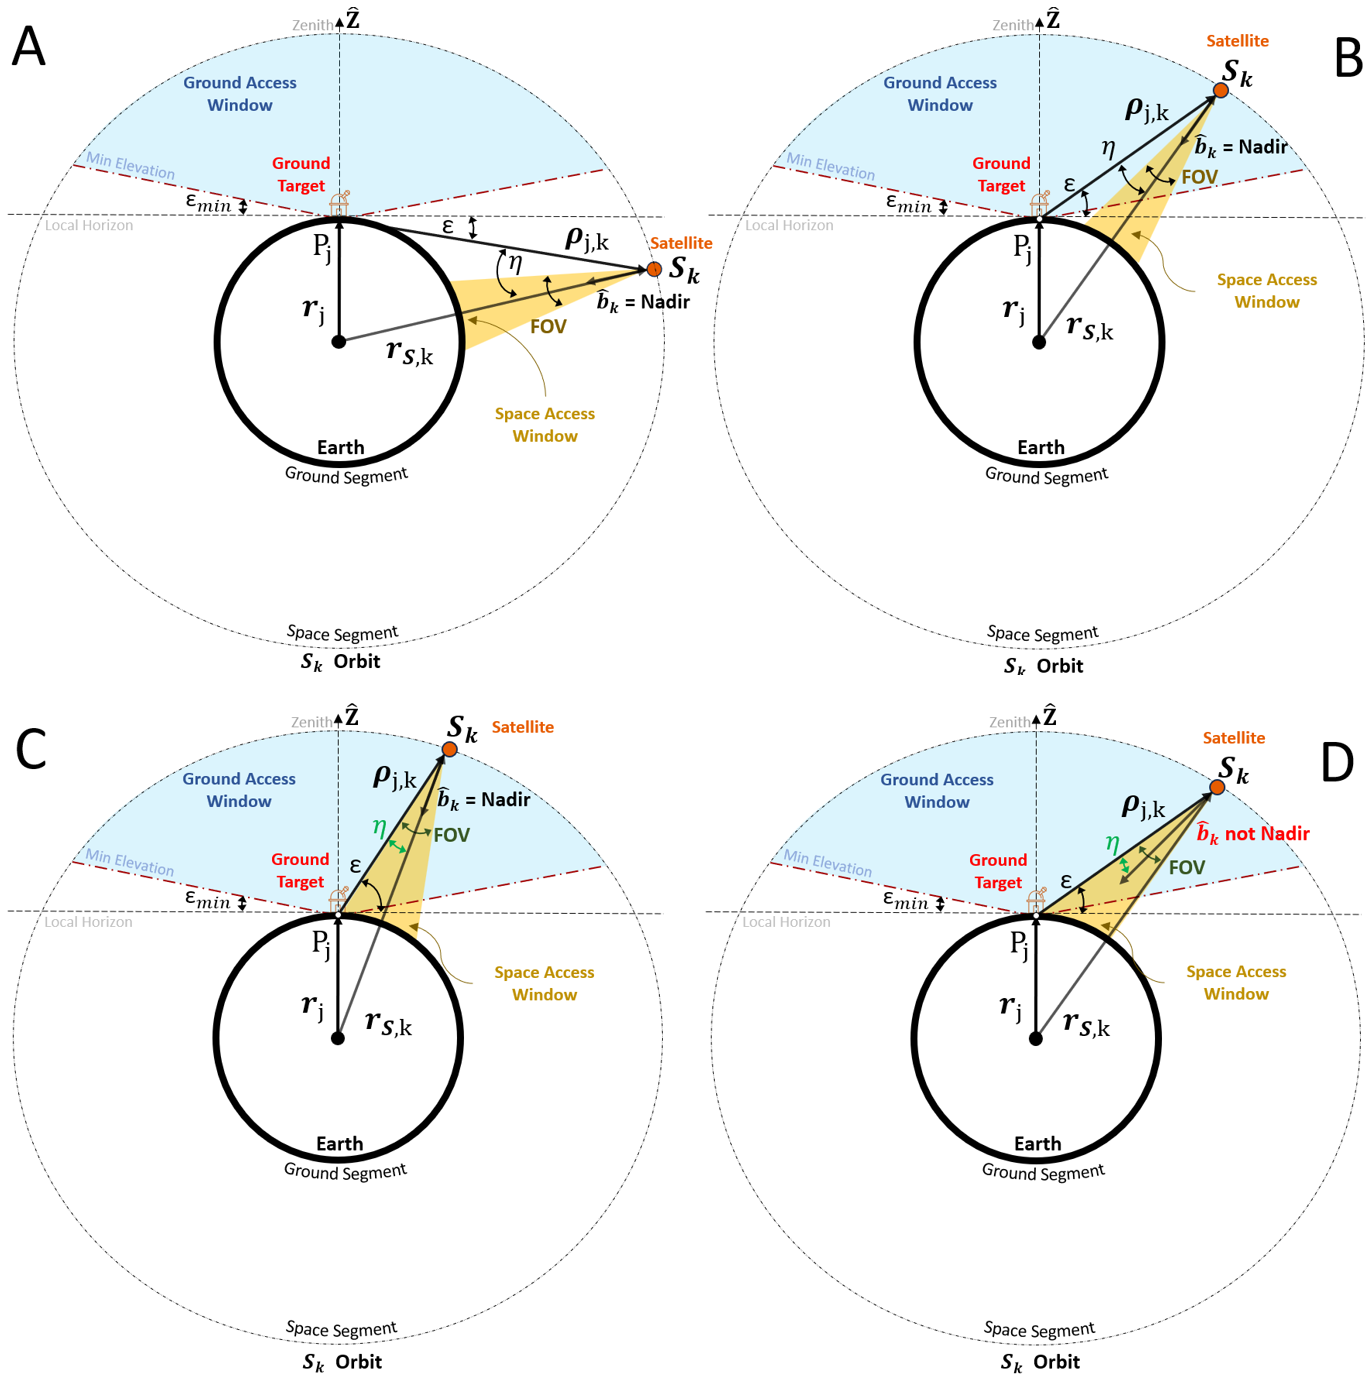
\includegraphics[width=1\linewidth]{images/acess_window_configs.png}
    \caption{\footnotesize{Observational Access Windows configuration. The figure illustrates the interaction between the \textbf{Ground Access Window} (blue cone, defined by tange point $P_j$ and $\epsilon_{min}$) and the \textbf{Space Access Window} (yellow cone, defined by the sensor direction $\hat{b}_k, FOV, $$\eta_{max}$).
    \textbf{(A)} No access: satellite is below the local horizon.
    \textbf{(B)} Ground access, no space access: satellite is above the horizon but with FOV outside $P_j$, or $\eta > FOV$.
    \textbf{(C)} Space \& ground access: satellite see ground $P_j$, ($\epsilon > \epsilon_{min}$) \& ($\eta < FOV$).
    \textbf{(D)} Space \& ground access with pointing out of nadir: $S_k$ uses point mechanism to have valid angular view from $P_j$ $(\theta \leq FOV)$.}}
    \label{fig:access_window_configs}
\end{figure}

\subsection{Ground Segment Access Window ($\mathcal{W}_{ground}$)}
From the perspective of the target $P_j$, $P_j \in \mathcal{F}_{SEZ}$, the satellite $S_k$ must appear within a specific volume of the local sky to ensure a clear signal path. We define the Ground Access Window as the subset in the Topocentric frame $\mathcal{F}_{SEZ}$ where the elevation angle exceeds the minimum operational threshold $\epsilon_{min}$ (imposed by terrain geometric masking and atmospheric attenuation).

Mathematically, this domain is defined by the condition on the relative position vector $\vec{\rho}_{j,k}$ with the spacecraft:
\begin{equation}
    \mathcal{W}_{ground_{j,k}}(t) = \{ \vec{\rho}_{j,k} \in \mathcal{M} \mid \epsilon(\vec{\rho}_{j,k}) \geq \epsilon_{min} \}
\end{equation}
where $\epsilon(\vec{\rho}_{j,k})$ is the elevation calculation defined in the previous section.

\subsection{Space Segment Access Window ($\mathcal{W}_{space}$)}
From the perspective of the satellite $S_k$, the target $P_j$ must lie within the instrument's Field of View (FOV). We define the \textbf{Space Access Window} (or Sensor Cone) based on the instrument's half-cone angle $\eta_{max}$ (FOV limit) relative to the instantaneous boresight vector $\hat{\mathbf{b}}_k(t)$.

The \textbf{Off-Nadir Angle} $\eta_{k,j}$ is defined as the angle between the sensor boresight and the direction to the target (which is $-\vec{\rho}_{j,k}$ in the satellite frame):
\begin{equation}
    \eta_{k,j}(t) = \arccos\left( \frac{-\vec{\rho}_{j,k}(t) \cdot \hat{\mathbf{b}}_{k}(t)}{\| \vec{\rho}_{j,k}(t) \|} \right)
\label{eq:eta}
\end{equation}
The Space Access Window is therefore the volume where this angle satisfies the optical limit:
\begin{equation}
    \mathcal{W}_{space_{j,k}}(t) = \{ \vec{\rho} \in \mathcal{M} \mid \eta(\vec{\rho}_{j,k}, \hat{\mathbf{b}}_k(t)) \leq \eta_{max} \}
\end{equation}
\subsection{Total Visibility Condition}
A valid observation event $E_{obs}$ occurs at time $t$ if and only if the Line-of-Sight vector exists within the intersection of both domains. Formally:
\begin{equation}
    \text{Visible}(t) \iff \vec{\rho}_{j,k}(t) \in \left( \mathcal{W}_{ground_{j,k}}(t) \cap \mathcal{W}_{space_{j,k}}(t) \right)
\end{equation}
This is equivalent to the simultaneous satisfaction of the two scalar inequalities:
\begin{equation}
    \text{Observation Link} \ \mathcal{L}_{j,k}(t) \iff Visible
    \begin{cases} 
        \epsilon_{k,j}(t) \geq \epsilon_{min} =15^{\circ} & \text{(Ground Access Condition)} \\
        \eta_{k,j}(t) \leq \eta_{max} = 65^{\circ} & \text{(Space Access Condition)}
    \end{cases}
    \label{eq:observation_link_condition}
\end{equation}


\section{Principles of Orbital
Mechanics}\label{71-principles-of-orbital-mechanics}

This section introduces the mathematical representation of satellite trajectories and the key gravitational effect that shapes them. The six classical orbital elements describe the size, shape, and orientation of an orbit, while the Earth's equatorial bulge induces predictable secular drifts in the orbital plane. These drifts are not merely perturbations to be corrected --- they are the physical mechanism that makes Repeating Ground Track and Sun-Synchronous orbits possible.

% \begin{itemize}
% \item
%   Explain the six Keplerian orbital elements (a, e, i, Ω, ω, ν) and what they define.
%   \item Introduce the concept of the constellation coverage domain, and how we expect to check this coverage
% \item
%   Discuss key perturbations, focusing on the J2 effect
%   (Earth\textquotesingle s oblateness) and its role in causing nodal
%   precession, which is fundamental to Repeating Ground Track Orbit
%   (RGTO) and Sun-Synchronous Orbits (SSO).
% \item
%   Introduce the concept of a ground track and how it is determined by
%   the orbital period and Earth's rotation.
% \end{itemize}

\subsection{Classical Orbital Elements and Satellite State Vector}
\label{sec:classical_orbital_elements}

To define the trajectory in spacetime of the constellation $\mathcal{C}_{sat}$ (Sec.~\ref{sec:Constellation_observation_form}) within the manifold $\mathcal{M}$, we use the classical Keplerian representation. The state of each satellite $S_k$ is uniquely determined within the inertial reference frame $\mathcal{F}_{J2000}$ by the set of six orbital elements and a reference epoch $t_0$. This is the \textbf{Orbital State Element} vector $\vec{A}_k$ introduced in the constellation formalism, which characterizes the instantaneous geometry of the orbital plane and the position of the spacecraft relative to the Earth's equatorial plane and the reference direction (the First Point of Aries). As illustrated in Fig.~\ref{fig:orbital_elements}, the vector is defined as:
\begin{equation}
    \vec{A}_k = [a, e, i, \Omega, \omega, \nu, t_0]^T
    \label{eq:orbital_state_vector}
\end{equation}
where the orientation of the orbital plane is governed by the Right Ascension of the Ascending Node (RAAN) $\Omega$, the Inclination $i$, and the Argument of Periapsis $\omega$, while the instantaneous position within the orbit is given by the True Anomaly $\nu$. These seven parameters fully determine the satellite's trajectory over the Study Domains $\mathcal{D}$ and constitute the fundamental input to the simulation propagator.

\begin{figure}[H]
    \centering
    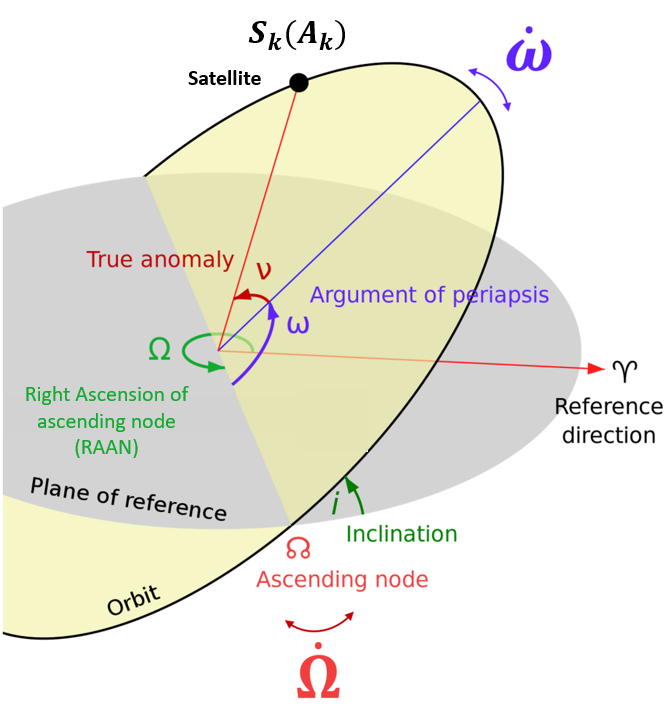
\includegraphics[width=0.5\linewidth]{images/orbital_elements_pertubed_due_J2.png}
    \caption{\footnotesize{Classical Keplerian orbital elements composing $\vec{A}_k$ (Eq.~\ref{eq:orbital_state_vector}): shape ($a$, $e$), plane orientation ($i$, $\Omega$, $\omega$), and in-orbit position ($\nu$) in $\mathcal{F}_{J2000}$. The secular variation (Section \ref{sec:perturbed_orbital_elements}) due to the $J_2$ perturbation: nodal regression rate $\dot{\Omega}$ (Eq.~\ref{eq:dot_Omega}), apidal precession $\dot{\omega}$ (Eq.~\ref{eq:dot_omega} }}
    \label{fig:orbital_elements}
\end{figure}


%===================================================
\section{Gravitational Perturbations and the Geopotential Model}
\label{sec:geopotentialmodel}
%===================================================

Gravitational perturbations caused by Earth's oblateness are a classical problem in astrodynamics.  The non-spherical mass distribution of the Earth---principally the equatorial bulge of approximately 21\,km---gives rise to a gravitational potential that deviates from the idealised Keplerian case $U_0 = \mu/r$.  This potential is conventionally expanded as a series of spherical harmonics characterised by zonal, sectoral, and tesseral coefficients \cite{valladoFundamentalsAstrodynamicsApplications2001}; the complete derivation and the dominant harmonic terms are presented in Appendix~\ref{app:geopotential}.  Among all harmonic coefficients, the second zonal term $J_2 \approx 1.08263 \times 10^{-3}$ exceeds every other coefficient by approximately three orders of magnitude, making it the single most important perturbation for LEO mission design.  The key practical results---the secular drift rates of the ascending node $\dot{\Omega}$, the argument of perigee $\dot{\omega}$, and the mean anomaly $\dot{M}$ induced by $J_2$---are derived below, as they directly determine the Repeating Ground Track Orbit (RGTO) resonance condition used throughout this work.



%===================================================
\subsection{Perturbed Orbital Elements due to \texorpdfstring{$J_2$}{J2}}
\label{sec:perturbed_orbital_elements}
%===================================================

The $J_2$ potential (Appendix~\ref{app:geopotential}) introduces secular rates of change in three of the Keplerian elements within $\vec{A}_k$. Denoting $p = a(1 - e^2)$ as the semi-latus rectum, first-order perturbation theory yields \cite{valladoFundamentalsAstrodynamicsApplications2001}:

\begin{equation}
    \dot{\omega} \;=\; \frac{3}{2}\,J_2
        \left(\frac{R_{\oplus}}{p}\right)^{\!2}
        \sqrt{\frac{\mu_{\oplus}}{a^3}}
        \left[2 - \tfrac{5}{2}\sin^2 i\right],
    \label{eq:dot_omega}
\end{equation}
\begin{equation}
    \dot{\Omega} \;=\; -\frac{3}{2}\,J_2
        \left(\frac{R_{\oplus}}{p}\right)^{\!2}
        \sqrt{\frac{\mu_{\oplus}}{a^3}}
        \cos i,
    \label{eq:dot_Omega}
\end{equation}
\begin{equation}
    \dot{M} \;=\; \sqrt{\frac{\mu_{\oplus}}{a^3}}
        \left[1 - \frac{3}{2}\,J_2
            \left(\frac{R_{\oplus}}{p}\right)^{\!2}
            \sqrt{1 - e^2}
            \left(\tfrac{3}{2}\sin^2 i - 1\right)\right].
    \label{eq:dot_M}
\end{equation}

These secular drifts and their physical consequences for mission design are summarised below. The illustration of this elements are shown in Figure \ref{fig:orbital_elements}.

\paragraph{\textbf{Nodal regression} $\dot{\Omega}$ }
 The ascending node $\Omega$ precesses at a constant rate determined by $a$, $e$, and $i$. For prograde orbits ($i < 90°$) the precession is westward; retrograde orbits ($i > 90°$) produce eastward drift. This rate is the determining factor for both Sun-Synchronous Orbits (SSO) and the resonance condition of Repeating Ground Track (RGT) orbits.
\paragraph{\textbf{Apsidal precession} $\dot{\omega}$}
 The argument of periapsis rotates in the orbital plane. At the \emph{critical inclination} $i \approx 63.4°$ (or $116.6°$), $\dot{\omega} = 0$, making the apoapsis location fixed, a property exploited by Molniya and Tundra orbits and by Flower Constellations using elliptical orbits.
\paragraph{\textbf{Mean-motion correction} $\dot{M}$}
 The effective mean motion departs from the Keplerian value $\sqrt{\mu_\oplus/a^3}$, modifying the satellite's nodal period relative to the nominal two-body case.


These secular rates constitute the astrodynamic foundation for the orbit design methodology developed in the next sections.

%===================================================
\subsection{Geopotential Scope of This Work}
\label{sec:otherharmonics}
%===================================================

Given the dominance of $J_2$ established above (Table~\ref{tab:harmonic_coefficients}), this work adopts two types of force model implementation:

\begin{enumerate}
    \item \textbf{Analytical design}: $J_2$ perturbation alone is for the derivation of the RGTO orbital state (semi-major axis, inclination, and nodal periods). This approximation is valid for defining the satellite's initial state because all other coefficients of the potential perturbation are at least three orders of magnitude smaller. 
    \item \textbf{High-fidelity simulation}: the numerical propagation in GMAT employs a complete force model --- gravitational, third-body, and atmospheric drag;  whose configuration is detailed in the simulation methodology chapter.
\end{enumerate}

\section{Earth Observation Orbits Candidates}
\label{72-earth_orbservation_orbit_candidates}

% """""""improve"
% Orbits are divided in classifications primarly defined by the altitude
% The classcombination of the requirements  of optical quality $GSD=6m/px$, limitsthe altitude 

% \textbf{temporal resolution $\mathbf{{t_{revisit} ≤ 30}}$} minutes and a \textbf{spatial resolution\textbf{ }$\mathbf{{GSD \approx 6 \text{ \textbf{m/pixel}}}}$  }would \textit{significantly improve the accuracy of fire model predictions}\inlineReq{R7}, \inlineReq{R8},

% Repeating Ground-Track Orbits (RGTO) are a class of orbits with specific orbital parameters that ensure the satellite’s ground track over Earth’s surface repeats after a fixed period. This design ensures consistent coverage of areas of interest and predictable revisit times. Furthermore, researchers have \textbf{identified RGTO as the optimal Low Earth Orbit (LEO) type of orbit for minimizing revisit intervals} \autocite{hansonDesigningGoodPartial1990}. Consequently, RGTO serve as the fundamental building blocks for designing LEO \emph{satellite constellations with rapid revisit capabilities}.

% As demonstrated in the coverage chapter, satellites in LEO are the choice of this project for high revisit rate constellation designs, as they provide the \emph{necessary spatial resolution} for wildfire monitoring. Therefore, the following sections will focus \emph{only on LEO circular orbit types}. %TODO: Add chapter reference to coverage chapter

% The following sections establish key physical principles underlying RGTO design, illustrating how these orbits enhance satellite coverage and revisit intervals for Earth observation missions. The RGTO astrodynamics theory presented here is inspired by \citeauthor{leeSatelliteConstellationPattern2020}'s work on Complex Coverage Constellations \autocite{leeSatelliteConstellationPattern2020}.""""


The GSD requirement of $\leq 6$\,m\,px$^{-1}$ constrains the observation altitude to the LEO regime, where the reduced distance delivers the spatial resolution unavailable from MEO or GEO.  Amongst LEO orbit types, the Repeating Ground Track Orbit (RGTO) is selected as the primary orbit family for this mission: it is identified in the literature as the optimal LEO orbit type for minimising revisit intervals over regional targets~\cite{hansonDesigningGoodPartial1990} and its resonance condition can be tuned to the target latitude (Coimbra, $\phi_{\text{lat}} = 40.2^{\circ}$\,N).  The Sun-Synchronous Orbit (SSO), the commercially dominant LEO orbit class for Earth observation, is retained as a comparison baseline; its full astrodynamic development and the quantitative RGTO--SSO comparison are presented in Appendix~\ref{app:sso_orbit}.  The remainder of this chapter develops the astrodynamic foundations of the RGTO.
 

\subsection{Repeating Ground Track Orbit (RGTO) Definition}
\label{72-RGTO_definition}
%-----------------------------------------------------------
% RGTO Orbit Definition
%-----------------------------------------------------------

A Repeating Ground Track Orbit (RGTO) is a class of orbits in which the satellite's sub-satellite ground track closes on itself after a fixed number of orbital revolutions, tracing an identical path over Earth's surface at every successive repeat cycle.  This property ensures consistent, predictable coverage of a target region and deterministic revisit intervals, which are essential for time-critical Earth observation missions.  Hanson~\textit{et al.}\ have formally identified RGTO as the optimal LEO orbit type for minimising revisit intervals over regional targets~\cite{hansonDesigningGoodPartial1990}; consequently, RGTO form the fundamental building block for designing LEO constellations with rapid revisit capability.  The astrodynamic theory developed below is inspired by \citeauthor{lee_satellite_2020}'s treatment of complex coverage constellations \cite{lee_satellite_2020}, a class of flower constellation \cite{mortariFlowerConstellationSet2008}.

\subsubsection{Resonance Condition}
\label{sec:rgto_resonance_condition}

The repeating-track property arises from a \textbf{compatibility} (resonance) condition between two rotating reference frames: the satellite's orbital frame $\mathcal{F}_S$, rotating at the satellite's mean motion $n$, and the Earth-fixed frame $\mathcal{F}_{\oplus}$, rotating at Earth's inertial rate $\omega_{\oplus}$.  Two such frames are compatible if their angular velocities satisfy the rational ratio
\begin{equation}
    N_P \, T_S = N_D \, T_G \,,
    \label{eq:rgto_compatibility}
\end{equation}
where $N_P \in \mathbb{Z}^+$ is the number of complete satellite nodal revolutions, $N_D \in \mathbb{Z}^+$ is the number of Earth rotation periods (nodal days), $T_S$ is the satellite nodal period, and $T_G$ is the Greenwich nodal period.  After $T_r = N_P\,T_S = N_D\,T_G$ the satellite and the Earth-fixed frame return simultaneously to their initial relative geometry, and the ground track closes.

Under the $J_2$ secular perturbation (Sec.~\ref{sec:perturbed_orbital_elements}), the nodal periods depend on the slowly varying orbital elements:
\begin{equation}
    T_S = \frac{2\pi}{\dot{\omega} + \dot{M}}\,, \qquad
    T_G = \frac{2\pi}{\omega_{\oplus} - \dot{\Omega}}\,,
    \label{eq:rgto_nodal_periods}
\end{equation}
where $\dot{\Omega}$, $\dot{\omega}$, and $\dot{M}$ are the $J_2$-driven secular rates of the ascending node, argument of perigee, and mean anomaly, respectively.  The \textbf{period ratio}
\begin{equation}
    \tau \equiv \frac{N_P}{N_D} = \frac{T_G}{T_S}
    = \frac{\dot{\omega} + \dot{M}}{\omega_{\oplus} - \dot{\Omega}}
    \label{eq:rgto_period_ratio}
\end{equation}
uniquely identifies each RGTO family.  OFractions $N_P/N_D$ define distinct ground tracks; for instance $\tau = 10/2$ and $\tau = 5/1$ produce identical repeating patterns.

\subsubsection{RGTO Orbital Element Vector}
\label{sec:rgto_element_vector_def}

Because the semi-major axis $a$ is fully determined by the resonance condition once $\tau$, $e$, and $i$ are fixed,\ $a = a(\tau, e, i)$,  the period ratio $\tau$ replaces $a$ as the independent orbital design parameter.  The \textbf{RGTO orbital element vector} of satellite $S_k$ is therefore defined as
\begin{equation}
    \vec{\mathbf{A}}^{\,\mathrm{RGTO}}{}_{k} = \bigl[\tau,\; e,\; i,\; \Omega,\; \omega,\; \nu,\; t_0\bigr]^{T}\,,
    \label{eq:rgto_element_vector}
\end{equation}
which fully specifies the orbit of $S_k$ within its RGTO family.

\subsubsection{Semi-Major Axis from the Resonance Condition}
\label{sec:rgto_sma_iteration}

Given the resonance integers $N_P$ and $N_D$, the eccentricity $e$, and the inclination $i$, the semi-major axis $a$ is recovered through the iterative scheme of \citeauthor{ulybyshevSatelliteConstellationDesign2008}~\cite{ulybyshevSatelliteConstellationDesign2008}.  An initial Keplerian estimate is obtained from the unperturbed mean motion:
\begin{equation}
    a_0 = \left(\frac{\mu_{\oplus}}{n_0^{2}}\right)^{1/3}, \qquad
    n_0 = \frac{N_P}{N_D}\,\omega_{\oplus}\,,
    \label{eq:rgto_a0_guess}
\end{equation}
where $\omega_{\oplus}$ is Earth's inertial rotation rate.  The $J_2$-corrected value is then refined iteratively:
\begin{equation}
    a_{k+1} = a_0
    \left[1 + \frac{3}{4}\,J_2\!\left(\frac{R_{\oplus}}{a_k}\right)^{\!2}
          \bigl(2 - 3\sin^{2} i\bigr)\right]^{2/3}
    \!\cdot\!
    \left[1 - \frac{3}{4}\,J_2\!\left(\frac{R_{\oplus}}{a_k}\right)^{\!2}
          \!\left(1 + \frac{2\,N_P}{N_D}\cos i - 5\cos^{2} i\right)\right]^{2/3}
    \label{eq:rgto_sma_iteration}
\end{equation}
until convergence $|a_{k+1} - a_k| < \varepsilon$ is reached..  Once $a$ is known, the nodal periods $T_S$ and $T_G$ in Eq.~\eqref{eq:rgto_nodal_periods} and the secular perturbation rates $\dot{\Omega}$, $\dot{\omega}$, $\dot{M}$ follow directly from the expressions derived in Sec.~\ref{sec:perturbed_orbital_elements}.



\subsection{Sun-Synchronous Orbit (SSO)}

A Sun-Synchronous Orbit (SSO) is a near-polar, retrograde orbit ($i > 90^{\circ}$) whose orbital plane precesses eastward at exactly the mean angular rate of the Earth around the Sun, preserving a constant solar-illumination geometry throughout the year.  This constant illumination makes SSOs the predominant choice for optical and multispectral Earth-observation missions and the most commercially accessible LEO orbit class via rideshare launches.  The complete SSO astrodynamic development---including the sun-synchronous condition, the inclination--altitude design equations, and the orbital element vector---is presented in Appendix~\ref{app:sso_orbit}.

With the observation geometry formalised and the astrodynamic foundations in place, the next chapter applies these tools to the mission design. The resonance condition derived here is used to generate the family of Repeating Ground Track Orbit modes tuned to continental Portugal, and a parametric coverage study over that orbit family selects the minimum viable constellation configuration.




% --- Chapter 8: Constellation Design and Optimization for Wildfire Monitoring in Portugal

\chapter{Constellation Architecture Design
}\label{73-constellation-design-architectures}

This chapter translates the orbital mechanics framework developed in Chapter~\ref{chp:baslie_orbit_metrics} into a concrete constellation design.  Section~\ref{chp:baslie_orbit_metrics} explores the RGTO resonance design space to select the optimal seed mode and evaluates its single-satellite temporal signature over 1-day, 7-day, and 30-day horizons, including station-keeping implications; a parallel SSO seed and quantitative RGTO--SSO comparison are documented in Appendix~\ref{app:sso_orbit}.  Section~\ref{73-constellation-architectures-design} extends the single-orbit analysis to a full Walker RGTO constellation, defining the plane count and satellite phasing needed to satisfy the revisit and coverage requirements over the core study domain $\mathcal{D}_{\mathrm{core}}$.

% \begin{itemize}
% \item
%   Introduce the concept of a satellite constellation as a means to
%   improve temporal coverage.
% \item
%   Explain the fundamental constellation patterns:{ -{ -

%   \begin{itemize}
%   \item
%     \textbf{Walker Star/Delta:} Describe this as a common method for
%     achieving uniform, global coverage by distributing satellites across; =
%     multiple, evenly spaced orbital planes. Define the key parameters.
%     (T/P/F: Total satellites/Planes/Phasing).
%   \item
%     \textbf{Flower Constellations:} Briefly introduce this as a more
%     advanced concept using circular orbits to create repeating ground
%     tracks over specific regions, allowing for targeted coverage. Say that it is used as an initial configuration condition, considering only J2 perturbation, and later, other perturbations are added for a more realistic simulation in cases considering lifetime and drag. But reduce the perturbation order to simplify the simulation and reduce computational cost.
%   \item
%     \textbf{Regional Constellations:} Explain how to Repeating Ground
%     Track Orbits and the Flower Constellations Concept to optimize
%     revisit time over a region.
%   \end{itemize}
% \end{itemize}


% \chapter{Constellation Architecture Trade-Off and
% Selection}\label{chapter-8-constellation-architecture-trade-off-and-selection}

% \begin{quote}
% \textbf{Writing Guide \& Methodological Focus:}

% \begin{itemize}
% \item
%   \textbf{Objective:} To present the core original work of the thesis:
%   the simulation and analysis of{ -ifferent constellation designs.
% \item
%   \textbf{Method:} State the options, show the results for each, and
%   then compare them to make a final, justified selection.
% \item
%   \textbf{Checkpoint:} Having rigorously tested the candidate
%   architectures and chosen a final design that is clearly the most
%   efficient solution?
% \end{itemize}
% \end{quote}

% \section{Orbit Class
% Selection}\label{81-orbit-class-selection}

% % \begin{itemize}
% % \item
% %   Briefly reiterate why circular LEO is the only viable option to meet
% %   the GSD requirement, referencing the analysis in Chapter 7.
% % \end{itemize}

% As analyzed in Chapter \ref{72-earth_orbservation_orbit_candidates}, due to the mission constraints evaluated during this work development, only two types of orbits are considered for the constellation design, the Repeating Ground Track Orbits (RGTO) and the Sun-Synchronous Orbits (SSO). This section will focus on a brief comparison between RGTO Vs SSO orbits during the propagation of it's orbits for one day.
% The state vectors to chose the candidate which decreases the number of satlelites and improve the




% \section{Candidate Constellation
% Configurations}\label{82-candidate-constellation-configurations}

% \begin{itemize}
% \item
%   Formally define the architectures you will test, specifying the design
%   parameters you will vary.

%   \begin{itemize}
%   \item
%     \textbf{Architecture A (Walker Delta):} Test various T/P/F
%     combinations for this baseline global coverage model.
%   \item
%     \textbf{Architecture B (Repeating Ground Track Orbits Optimized
%     Inclined Orbits):} Test constellations with inclinations
%     specifically chosen to maximize passes over
%     Portugal\textquotesingle s latitude, taking advantage of
%     Earth\textquotesingle s gravitational perturbations.
%   \item
%     \textbf{Architecture C (Sun-Synchronous Phased Orbits):} Test a
%     constellation in a common SSO plane to evaluate performance for a
%     specific observation time.
%   \item
%     \textbf{Architecture D (Tip-Cue, Ra--Sekhmet Framework):} \textit{[Note: Introduce the mythological "Tip and Cue" naming here. High-Obs (Ra) $\rightarrow$ Low-Act (Sekhmet).]} Test a hybrid layer approach where a high-altitude asset cues the LEO fleet.
%   \end{itemize}
% \end{itemize}

% \section{Performance Simulation and
% Results}\label{83-performance-simulation-and-results}

% \begin{itemize}
% \item
%   Present the outputs of the simulations clearly.
% \item
%   For each architecture, show how the Key Parameters Metrics (KPMs).
% \item
%   (maximum work Focus)Use maps to visualize coverage statistics over Portugal for the most
%   promising configurations.
% \end{itemize}

\section{Mission Modeling And Analysis Methodological Workflow}
\label{sec:mission_modeling_workflow}

Before deriving the orbit selection metrics that follow, this section outlines the simulation and analysis pipeline from which all quantitative results in this chapter and subsequent chapters are produced.  The workflow, illustrated in Fig.~\ref{fig:mission_modeling_workflow}, chains orbit computation, high-fidelity propagation, and observation-geometry evaluation into a single reproducible process; each subsequent section applies one or more stages of this pipeline to progressively build the constellation design.

\begin{figure}[H]
    \centering
    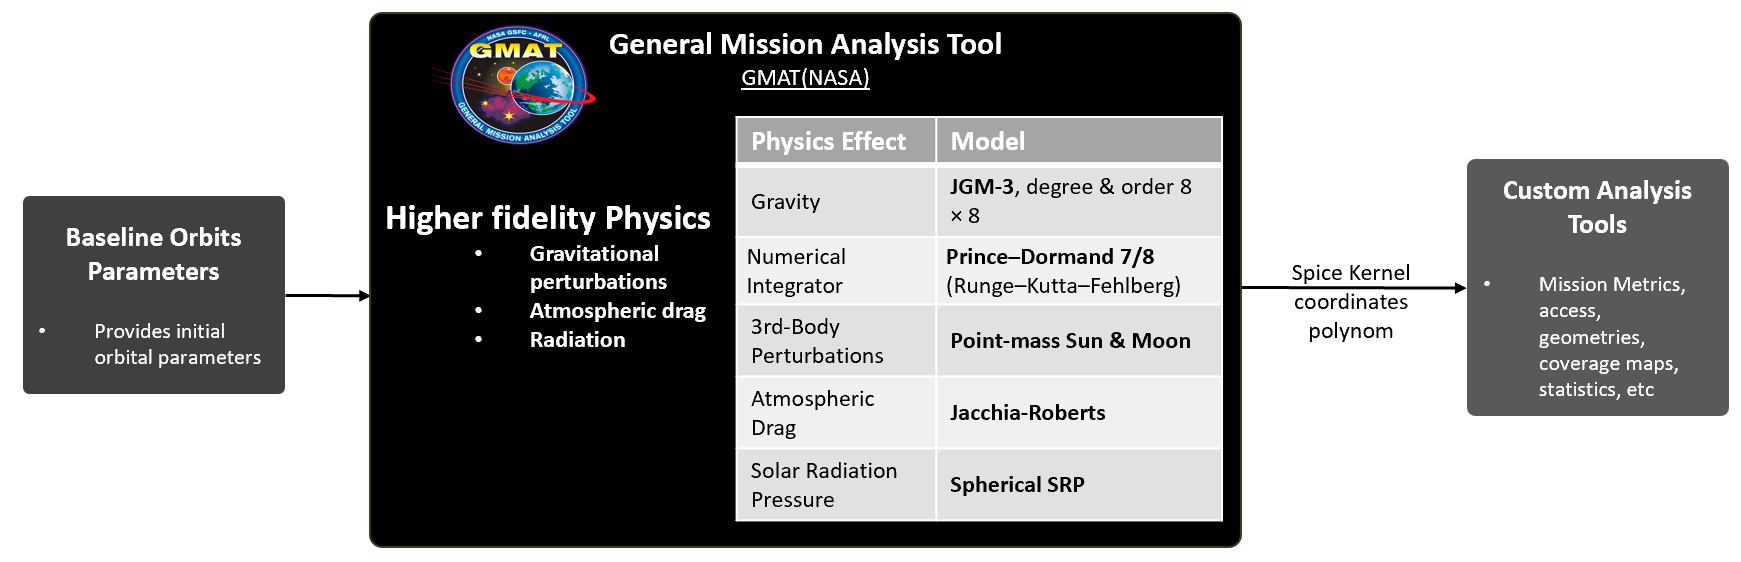
\includegraphics[width=1\linewidth]{images/mission_modeling_workflow.png}
    \caption{\footnotesize{Mission modeling and analysis workflow.  Baseline orbit parameters (Keplerian elements from the RGTO resonance analysis) are propagated in GMAT with high-fidelity physics (JGM-3 $8\times8$ gravity, Jacchia--Roberts drag, SRP, Moon/Sun perturbations).  The resulting SPICE ephemeris files are then ingested by the custom Python analysis tools to compute observation-link geometry, coverage maps, and performance statistics.}}
    \label{fig:mission_modeling_workflow}
\end{figure}

The pipeline, implemented in \texttt{Python}, comprises three stages:

\begin{enumerate}[label=\textbf{Stage~\arabic*.}, leftmargin=*, itemsep=4pt]
    \item \emph{Analytical orbit computation.}  A custom \texttt{RTGOrbit} class uses \texttt{Astropy} physical constants and \texttt{SciPy} root-finding to solve the $J_2$-perturbed resonance condition, yielding the initial Keplerian elements for each candidate orbit.

    \item \emph{High-fidelity propagation.}  The elements are imported into NASA's General Mission Analysis Tool (GMAT), which propagates the 12U~CubeSat with a Prince--Dormand~7(8) integrator, the JGM-3 $8\times8$ gravity field, Jacchia--Roberts atmospheric drag, solar radiation pressure, Sun and Moon point-mass perturbations, and relativistic corrections, using the spacecraft parameters in Table~\ref{tab:cubesat_params}.  GMAT exports the ephemerides as SPICE Binary~SPK (\texttt{.bsp}) kernels.

    \item \emph{Observation-geometry analysis.}  A custom framework loads the SPK kernels via \texttt{SpiceyPy}, transforms spacecraft states through GCRS/ITRS frames (\texttt{Astropy} \texttt{SkyCoord}), and evaluates visibility over a latitude--longitude ground grid at a fixed sampling step of $\Delta t = 10$\,s.  Each grid point undergoes a $\mathcal{F}_{J2000} \!\to\! \mathcal{F}_{SEZ}$ coordinate transformation followed by the elevation and off-nadir angle tests of the observation-link condition (Eq.~\eqref{eq:observation_link_condition}).
\end{enumerate}

\begin{table}[H]
    \centering
    \caption{\footnotesize{12U CubeSat physical parameters used in the GMAT propagation model.}}
    \label{tab:cubesat_params}
    \footnotesize
    \begin{tabular}{lcc}
        \hline
        \textbf{Parameter} & \textbf{Value} & \textbf{Unit} \\
        \hline
        Dry mass              & 18   & kg          \\
        Drag coefficient $C_d$ & 2.2  & --          \\
        Reflectivity coefficient $C_r$ & 1.3  & --  \\
        Drag area             & 0.1  & m$^{2}$     \\
        SRP area              & 0.5  & m$^{2}$     \\
        \hline
    \end{tabular}
\end{table}

The ground grid used throughout this work comprises up to $120 \times 360 = 43\,200$~points, and the GMAT ephemerides are sampled at $\Delta t = 10$\,s, yielding $N_t = 8\,640$ time steps per satellite per day.  For $N_{\mathrm{sat}=15}$ satellites the third stage must therefore evaluate
\begin{equation}
    N_{\mathrm{eval}} = N_{\mathrm{sat}} \times N_{\mathrm{grid}} \times N_t = 15 \times 43\,200 \times 8\,640 \approx 5.60 \times 10^{9} \;\text{visibility checks per day,}
    \label{eq:visibility_eval_count}
\end{equation}
visibility checks per day of propagation, each involving a coordinate transformation and the observation-link tests of Eq.~\eqref{eq:observation_link_condition}; scaling to multi-day,  monthly, annually horizons increases the workload proportionally.  Designing, implementing, and optimising this computational pipeline to handle such volumes constituted the main engineering challenge of this thesis, spanning more than one year of iterative development.  To manage the computational load the framework employs CPU-level parallelism (\texttt{ProcessPoolExecutor}, batching target points across all available cores) and optionally offloads the vectorised visibility kernel to GPU via \texttt{CuPy} (NVIDIA CUDA), reducing a single global coverage map from the order of days on a single core to several hours with multiprocessing, or to a few minutes when the GPU path is used\footnote{All simulations reported in this thesis were executed on a workstation equipped with an Intel Core i9-13900KF processor (24~cores / 32~threads, up to 5.8\,GHz), 128\,GB DDR5 RAM, and an NVIDIA GeForce RTX~4070 GPU (12\,GB GDDR6X).}.  A more detailed description of this computational framework is left for future work.




\section{Baseline Orbits Metrics Comparison}
\label{chp:baslie_orbit_metrics}

The earth observation orbit candidates were defined in Chapter~\ref{72-earth_orbservation_orbit_candidates}, where the Repeating Ground Track Orbit (RGTO) was identified as the primary orbit family for this mission.  This section presents the RGTO seed orbit metrics---resonance space, altitude--inclination selection, and single-satellite temporal signature---that drive the constellation sizing.  A parallel Sun-Synchronous Orbit (SSO) seed and the quantitative RGTO--SSO comparison are documented in Appendix~\ref{sct-SSO_seed}.

\subsubsection{RGTO Resonance Space at Coimbra: Selecting the optimal seed orbit}
\label{sec:rgto_resonance_space_coimbra}

Varying the free parameters $(N_P,\, N_D,\, i)$ in $\vec{A}_{k,\mathrm{RGTO}}$ (Eq.~\eqref{eq:rgto_element_vector}) while holding $e \approx 0$ generates a family of resonance conditions in the altitude--inclination plane.  Each point on these curves satisfies the convergence criterion of Eq.~\eqref{eq:rgto_sma_iteration}, i.e.\ the sub-satellite ground track closes after exactly $N_D$ sidereal days.  Figure~\ref{fig:RGTO_ressonantSpace} maps this design space for repeat-cycle durations $N_D = 1$ through $6$\,days.  Shorter repeat cycles confine the feasible altitudes to a narrower inclination range, which is desirable because it maximises the daily revisit rate over a given target latitude.

The analysis is now restricted to the single-day repeat case ($N_D = 1$), which minimises the revisit period to approximately one sidereal day ($T_r \approx 0.98$\,d).  Applying the constraint $i = \phi_{\text{lat}} = 40.2^{\circ}$ (Coimbra, Table~\ref{tab:pt_coords}) yields a discrete set of candidate altitudes---one per integer $N_P$---shown in Fig.~\ref{fig:RGTO_1day_resonance}.  Modes $N_P = 12$--$13$ fall in the MEO range ($h > 800$\,km), where the larger Earth-disc distance degrades the Ground Sample Distance (GSD).  Mode $N_P = 16$ descends into the VLEO regime ($h < 450$\,km), where atmospheric drag severely limits mission lifetime without continuous station-keeping.  The mode $\tau = 15/1$ at $h \approx 488$\,km occupies the lower Earth Observation band, offering a favourable trade-off between spatial resolution, mission lifetime, and temporal coverage ($T_S \approx 5652$\,s per revolution).

\begin{figure}
    \centering
    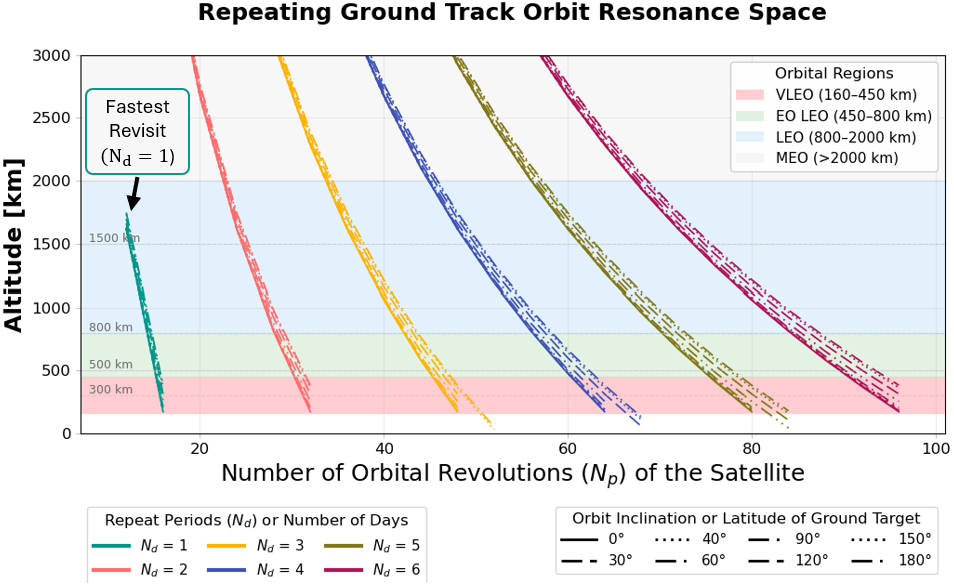
\includegraphics[width=0.92\linewidth]{images/RGTO_ressonantSpace.png}
    \caption{\footnotesize{RGTO resonance design space: orbital altitude $h$ as a function of inclination $i$ for repeat-cycle durations $N_D = 1$ through $6$\,days.  Each curve corresponds to a fixed number of revolutions per cycle~$N_P$; increasing $N_P$ lowers the orbital altitude.  Shorter repeat cycles concentrate the feasible altitude--inclination pairs into a narrower band, enabling faster ground-track revisit.}}
    \label{fig:RGTO_ressonantSpace}
\end{figure}

\begin{figure}
    \centering
    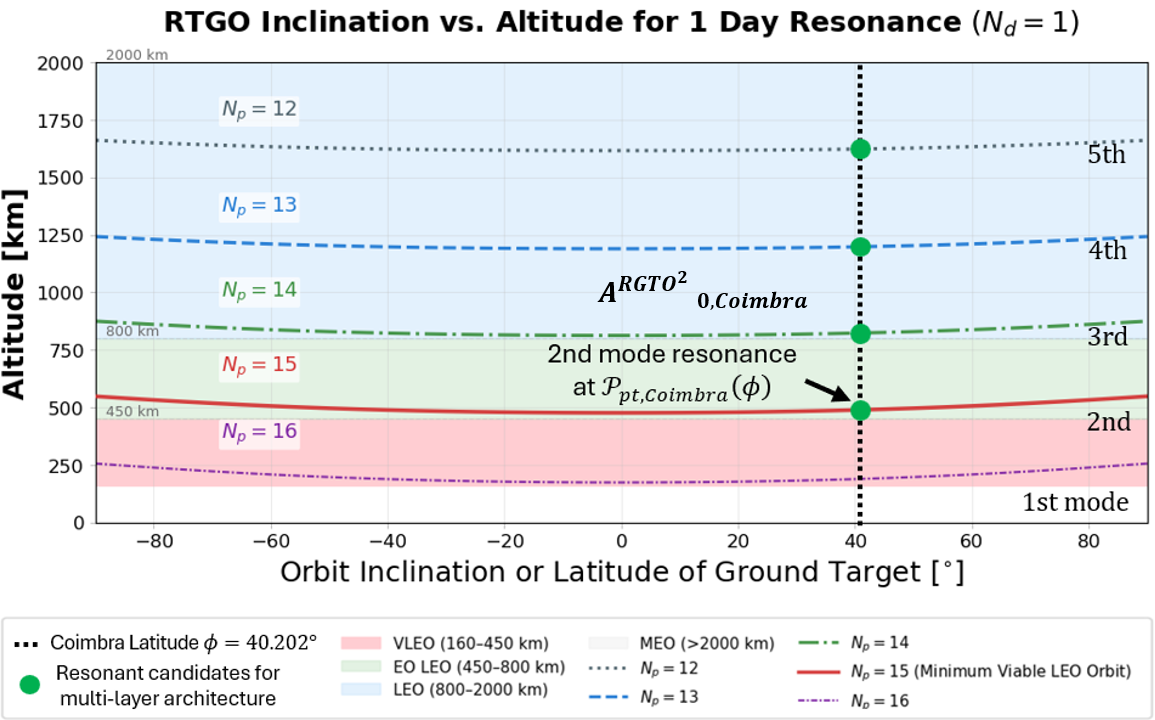
\includegraphics[width=0.92\linewidth]{images/RGTO_1day_resonance.png}
    \caption{\footnotesize{Detail of the $N_D = 1$ resonance space showing altitude versus inclination for $N_P \in [12,\,16]$.  The vertical line at $i = \phi_{\text{lat}} = 40.2^{\circ}$ (Coimbra latitude, Table~\ref{tab:pt_coords}) intersects the resonance curves, defining the five candidate modes listed in Table~\ref{tab:rgto_parameters_coimbra}.  Shaded altitude bands indicate the Very Low Earth Orbit (VLEO, $h < 450$\,km), Earth Observation (EO, $450$--$800$\,km), and Medium Earth Orbit (MEO, $h > 800$\,km) regimes.  The selected mode $\tau = 15/1$ ($h \approx 488$\,km) lies at the lower bound of the EO band.}}
    \label{fig:RGTO_1day_resonance}
\end{figure}



for the constellation architecture: the $\tau = 15/1$ mode at $h \approx 488$\,km.  This configuration provides the best trade-off between fast revisit (one sidereal day), high spatial resolution (lower EO band), and viable mission lifetime (manageable atmospheric drag).  The complete set of derived orbital parameters for all five candidate modes is presented in Sec.~\ref{sec:rgto_parametric_results}.

From this analysis we create a nomenclature to define the orbital element vector of a RGTO of mode $n$ with index k resonating with an Earth point target P as $\vec{\mathbf{A}}^{\,\mathrm{RGTO}^{\, n}}{}_{k,\,\mathrm{P}}$, where $n$ is the integer number modes of this resonant orbit, with n=1 the closest to the planet surface.

Figure~\ref{fig:RGTO_1day_resonance} show the optimal seed case is modeled by the orbital element vector k=0 describing a RGTO of second mode at Coimbra defined as:
\begin{equation}
  \vec{\mathbf{A}}^{\,\mathrm{RGTO}^{\,2}}{}_{0,\,\mathrm{Coimbra}} = \bigl[15/1,\; 0.001,\; 40.2033^{\circ},\; 0^{\circ},\; 0^{\circ},\; 0^{\circ} ,\; 0s\bigr]^{T}
\label{eq:RGTO_2_coimbra}
\end{equation}
The complete set of derived orbital parameters for all five candidate modes is presented in Sec.~\ref{sec:rgto_parametric_results}.

\subsubsection{RGTO Parametric Results at Coimbra}
\label{sec:rgto_parametric_results}

Table~\ref{tab:rgto_parameters_coimbra} summarises the derived orbital parameters for five candidate resonance orbits modes ($\tau = 12/1$ through $16/1$) evaluated at the Coimbra target latitude, table \ref{tab:pt_coords}, \reqRef{R14}.  All modes share the common initial conditions of been near circular orbit at the same plane and epoch.

\begin{table}[H]
\centering
\caption{\footnotesize{RGTO seed orbit parameters for five resonance modes at Coimbra ($\phi_{\text{lat}} \approx 40.20329^{\circ}$\,N).  Common conditions: $e = 0.001$, $\omega = 0^{\circ}$, $\Omega = 0^{\circ}$, $M = 0^{\circ}$.  The semi-major axis $a$ is obtained via the iterative scheme of Eq.~\eqref{eq:rgto_sma_iteration}; perturbation rates follow from the $J_2$ secular theory (Sec.~\ref{sec:perturbed_orbital_elements}).}}
\label{tab:rgto_parameters_coimbra}
\smallskip
\footnotesize
\setlength{\tabcolsep}{4pt}
\begin{tabular}{c l r r r r r r r r r}
\toprule
$n$
  & $\tau\;(N_P\!/N_D)$
  & $a$ [km]
  & $h$ [km]
  & $i$ [$^{\circ}$]
  & $T_S$ [s]
  & $T_G$ [s]
  & $T_r$ [d]
  & $\dot{\Omega}$ [rad\,s$^{-1}$]
  & $\dot{\omega}$ [rad\,s$^{-1}$]
  & $\dot{M}$ [rad\,s$^{-1}$] \\
\midrule
5 & 12/1 & 8000.90  & 1622.80 & 40.20329  & 7112  & 85\,350 & 0.9879  & $-6.95{\times}10^{-7}$ & $8.72{\times}10^{-7}$ & $8.83{\times}10^{-4}$ \\
4 & 13/1 & 7575.91  & 1197.81 & 40.220329  & 6552  & 85\,180 & 0.9859  & $-8.42{\times}10^{-7}$ & $1.06{\times}10^{-6}$ & $9.58{\times}10^{-4}$ \\
3 & 14/1 & 7200.84  & 822.74  & 40.20329  & 6071  & 84\,990 & 0.9837  & $-1.01{\times}10^{-6}$ & $1.26{\times}10^{-6}$ & $1.03{\times}10^{-3}$ \\
\rowcolor{green!15} {\bfseries 2} & {\bfseries 15/1$^{\dagger}$} & {\bfseries 6866.64}  & {\bfseries 488.54}  & {\bfseries 40.20329}  & {\bfseries 5652}  & {\bfseries 84\,780} & {\bfseries 0.9813}  & {\bfseries $-1.19{\times}10^{-6}$} & {\bfseries $1.49{\times}10^{-6}$} & {\bfseries $1.11{\times}10^{-3}$} \\
1 & 16/1 & 6566.35  & 188.25  & 40.20329  & 5285  & 84\,550 & 0.9786  & $-1.39{\times}10^{-6}$ & $1.74{\times}10^{-6}$ & $1.19{\times}10^{-3}$ \\
\bottomrule
\end{tabular}
\\[2pt]
{\footnotesize \parbox{0.97\linewidth}{$^{\dagger}$ Selected baseline RGTO seed candidate: this mode provides the best trade-off for fast revisit, maximum coverage over the core study domain $\mathcal{D}_{\mathrm{core}}$, and viable mission lifetime.}}
\label{tab:rgto_family_coimbra}
\end{table}

To validate the RGTO selection, the seed orbit was benchmarked against a Sun-Synchronous Orbit (SSO) baseline derived from SpaceX Transporter rideshare injection parameters ($a = 6904$\,km, $h \approx 525.9$\,km, $i_{\mathrm{SSO}} = 97.50^{\circ}$).  The full SSO seed derivation and the 7-day observation-link comparison are presented in Appendix~\ref{sct-rgto_vs_sso}.  The key finding is that the near-polar SSO crosses Coimbra's latitude at a steep angle with limited permanence time, whereas the RGTO ground track aligns with the target latitude, yielding approximately 1.75 times the daily coverage rate.  Consequently, an SSO-based constellation would require roughly twice as many satellites to achieve equivalent temporal coverage, confirming the RGTO as the preferred orbit class for this mission.

\section{Constellation Architectures Design}\label{73-constellation-architectures-design}

The selected seed orbit $\vec{\mathbf{A}}^{\,\mathrm{RGTO}^{\,2}}{}_{0,\,\mathrm{Coimbra}}$ (Eq.~\eqref{eq:rgto_element_vector}) is propagated over 1-day and 7-day windows to characterise its temporal coverage signature at the Coimbra ground station before addressing the full constellation.  Figures~\ref{fig:RGTO_maps_Coimbra_One_day}--\ref{fig:RGTO_metrics_Coimbra_Seven_days} present the ground-track geometry and the associated observation-link metrics; the revisit structure derived here drives the plane and satellite-count trade-off in the sections that follow.

\subsection{Single-Satellite Temporal Signature over 1-Day}
\label{sec:seed_1day_propagation}

The seed orbit is first propagated over a single day coinciding with the peak fire reference date (August~18, \reqRef{R16}) to characterise the repeating-ground-track geometry and the observation-link signature at Coimbra.

Figure~\ref{fig:RGTO_maps_Coimbra_One_day} presents the geometrical view.  The ground-track plot~(B) confirms the resonance condition: the sub-satellite trace overlaps itself precisely over the 1-day window.  At the latitude of Coimbra, the observation-link access boundary is marked by the blue dashed line, corresponding to the minimum elevation mask $\varepsilon_{\min} = 15^{\circ}$.  The sky plot~(A) displays the same passes in a polar azimuth--elevation diagram (elevation $0^{\circ}$ at the rim, $90^{\circ}$~=~zenith at the centre).  Four passes cross the Coimbra sky within a single day; they span approximately from 12:46 to 17:50~local time, and the closest nadir approach---the greenish-yellow trajectory---occurs near 15:00\,LT, coinciding with the peak fire observation window \reqRef{R35}.

The quantitative observation-link metrics are detailed in Fig.~\ref{fig:RGTO_metrics_Coimbra_One_day}.  Plot~(A) shows the visibility timeline: four successive passes satisfy the observation-link condition (Eq.~\ref{eq:observation_link_condition}), i.e.\ the logical conjunction of the ground-segment access $\varepsilon \geq \varepsilon_{\min} = 15^{\circ}$ and the space-segment access $\eta \leq \eta_{\max} = 65^{\circ}$.  The inter-revisit gap between consecutive passes is $t_{\mathrm{rev,RGTO}} \approx 99.23$\,min, and the four passes together form a single-day observation sequence window of $T_{\mathrm{seq,RGTO}} \approx 4$\,h\,57\,min.

Plot~(B) displays the elevation and distance profiles.  The elevation peaks vary across the four passes---from $\sim\!40^{\circ}$ for the first, through $\sim\!80^{\circ}$ and $\sim\!75^{\circ}$ for the second and third, down to $\sim\!25^{\circ}$ for the fourth---while the minimum slant distance reaches approximately 500\,km at closest approach.  All passes remain above $\varepsilon_{\min}$.

Plot~(C) presents the off-nadir angle~$\eta$ and the corresponding Ground Sample Distance on the right axis.  The off-nadir angle reaches minima of $\sim\!25^{\circ}$, $\sim\!10^{\circ}$, $\sim\!12^{\circ}$, and $\sim\!47^{\circ}$ for the four passes respectively, and the GSD remains below $6$\,m/pixel throughout, satisfying the spatial resolution requirement \reqRef{R8} under the paraxial GSD model Eq.~\ref{eq:gsd}.

The key outcome of this 1-day analysis is the identification of the seed temporal pattern: four passes clustered within a $\sim$5-hour window, separated by $\sim$99-minute gaps, leaving the remaining $\sim$19~hours of the day unobserved.  To extend coverage throughout the full day, this pattern can be replicated by introducing additional satellites in the same orbital plane, phased by a true-anomaly shift~$\Delta\nu$, such that their observation sequences fill the inter-sequence gaps.  Once a single plane achieves the target intra-plane revisit, the plane itself is replicated at different rotations around the reference orthogonal axis to map different RAAN values to cover the full sidereal day.  This two-level approach of populating a plane, then distributing planes, is developed in Section~\ref{sec:constellation_plane1}.

\begin{figure}
    \centering
    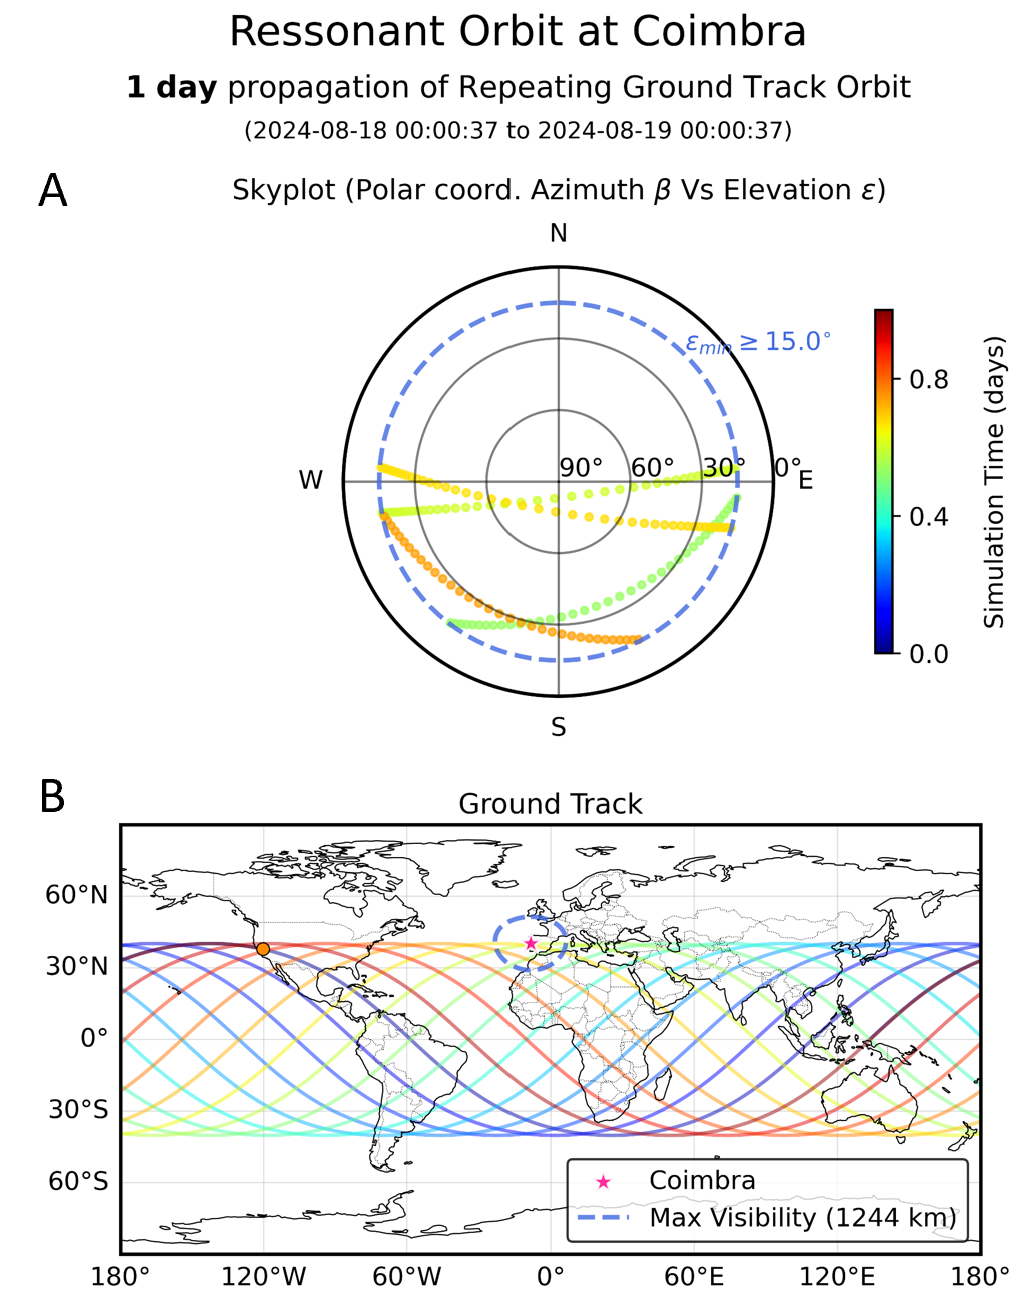
\includegraphics[width=0.9\linewidth]{images/RGTO_maps_Coimbra_One_day.png}
    \caption{1-day RGTO seed propagation over Coimbra ($\tau = 15/1$, $h \approx 488$\,km, $i = 40.2^{\circ}$, 2024 August~18) verifying resonance condition pattern.  \textbf{(A)}~Azimuth--elevation sky plot; four passes cross the sky between $\sim$12:46 and $\sim$17:50\,LT, with the near-nadir pass at $\sim$15:00\,LT.  \textbf{(B)}~Ground-track map; the blue dashed line marks the $\varepsilon_{\min} = 15^{\circ}$ observation-link access boundary.}
    \label{fig:RGTO_maps_Coimbra_One_day}
\end{figure}

\begin{figure}
    \centering
    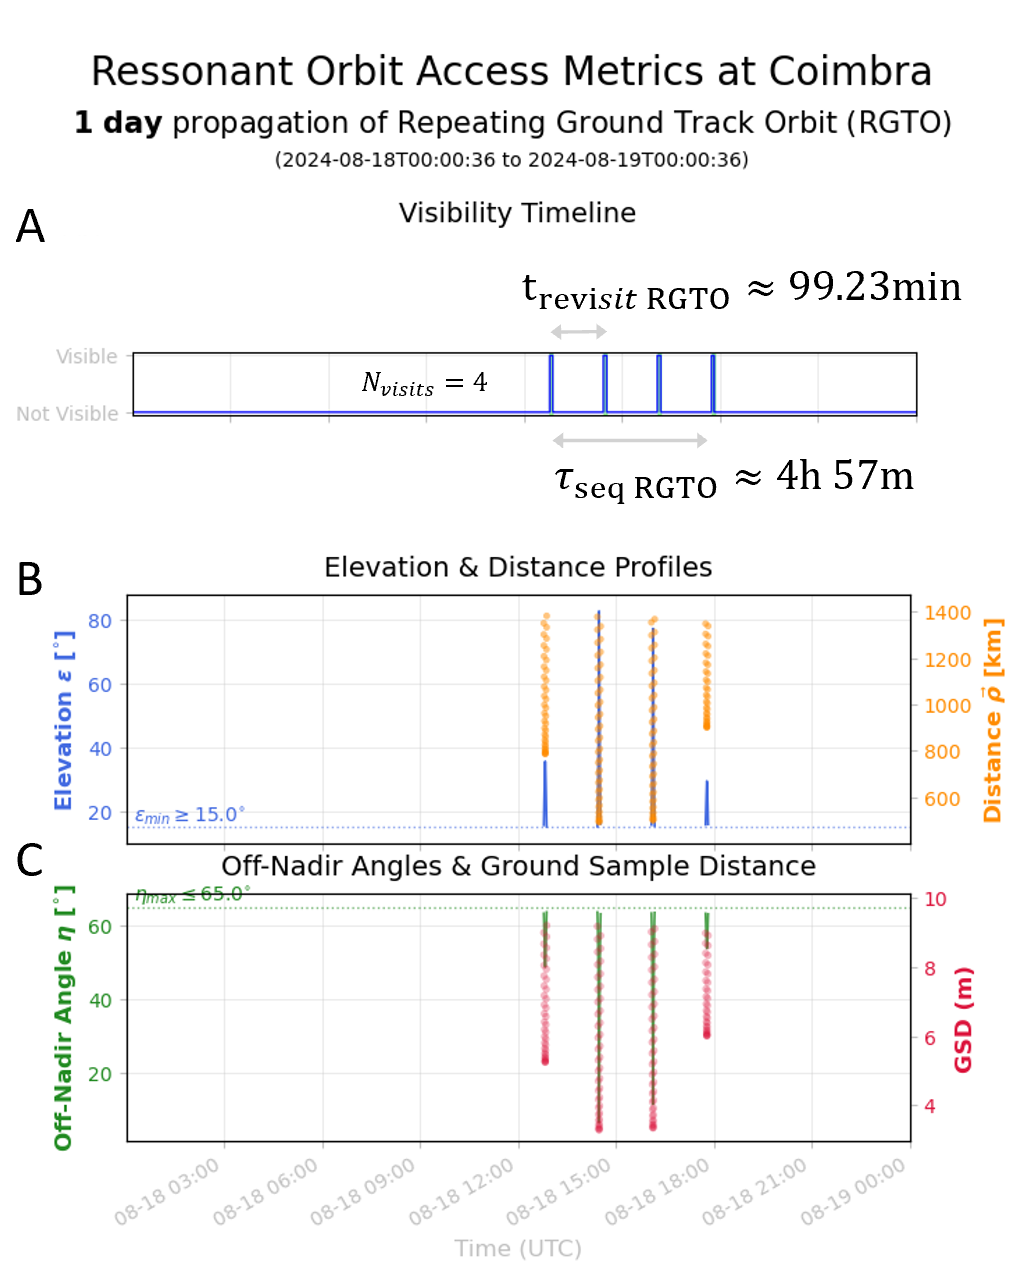
\includegraphics[width=1\linewidth]{images/RGTO_metrics_Coimbra_One_day.png}
    \caption{Observation-link metrics for the 1-day RGTO propagation at Coimbra.  \textbf{(A)}~Visibility timeline: four passes with inter-revisit gap $t_{\mathrm{rev,RGTO}} \approx 99.23$\,min forming a sequence window $T_{\mathrm{seq,RGTO}} \approx 4$\,h\,57\,min.  \textbf{(B)}~Elevation and slant-distance profiles.  \textbf{(C)}~Off-nadir angle~$\eta$ and GSD (right axis); GSD\,$< 6$\,m/pixel for all passes.}
    \label{fig:RGTO_metrics_Coimbra_One_day}
\end{figure}


\subsection{Single-Satellite Temporal Signature over 7-Days}
\label{sec:seed_7day_propagation}

The same seed orbit is propagated over a 7-day window to verify the persistence of the resonance pattern under atmospheric drag and $J_{8\times8}$ gravitational perturbations.  The ground-track and sky-plot maps for this period (Appendix~\ref{sec:appendix_7day_maps}, Fig.~\ref{fig:RGTO_maps_Coimbra_Seven_days}) confirm that the sub-satellite trace overlaps the 1-day pattern (Fig.~\ref{fig:RGTO_maps_Coimbra_One_day}) without appreciable drift, and the four-pass cluster recurs daily with consistent azimuth--elevation trajectories.

\begin{figure}
    \centering
    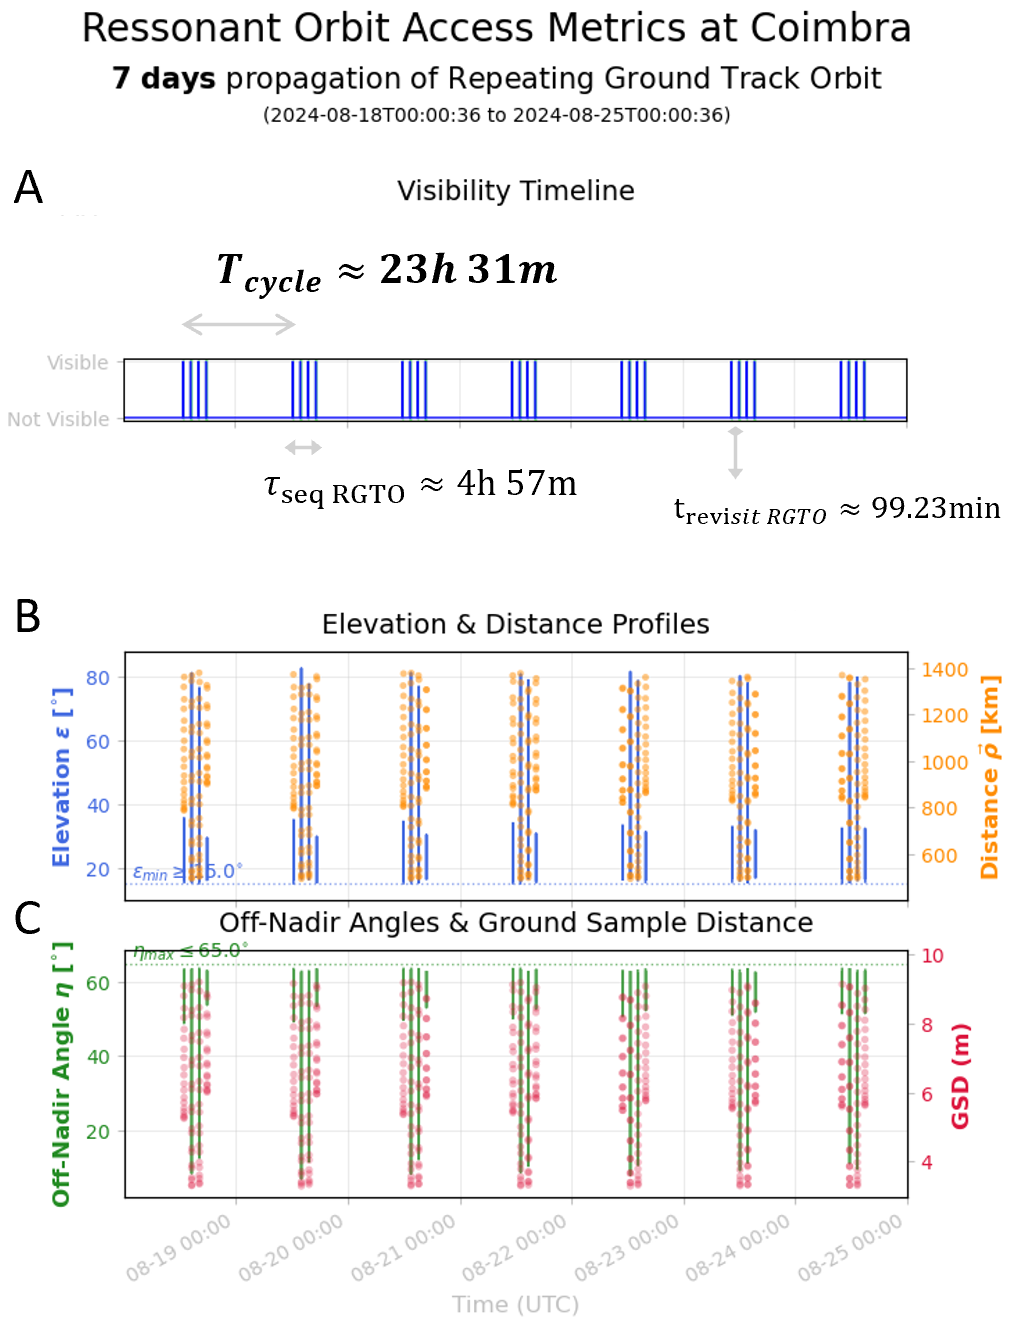
\includegraphics[width=1\linewidth]{images/RGTO_metrics_Coimbra_Seven_days.png}
    \caption{Observation-link metrics for the 7-day RGTO propagation at Coimbra.  \textbf{(A)}~Visibility timeline: the four-pass sequence repeats with $T_{\mathrm{rep,RGTO}} \approx 23$\,h\,30\,min (28~passes total).  \textbf{(B)}~Elevation and distance profiles across all passes.  \textbf{(C)}~Off-nadir angle and GSD; quality remains within the 1-day envelope.}
    \label{fig:RGTO_metrics_Coimbra_Seven_days}
\end{figure}

The observation-link metrics for the 7-day window (Fig.~\ref{fig:RGTO_metrics_Coimbra_Seven_days}) quantify this recurrence.  The visibility timeline~(A) shows the four-pass sequence repeating with a near-sidereal cycle $T_{\mathrm{rep,RGTO}} \approx 23$\,h\,30\,min, yielding 28~passes over 7~days (four per cycle).  The effective observation window per day remains $T_{\mathrm{seq,RGTO}} \approx 5$\,h, consistent with the 1-day result.  The elevation and distance profiles~(B) across all 28~passes show no degradation attributable to drag.  The off-nadir angle and GSD~(C) remain within the 1-day envelope, with GSD\,$< 6$\,m/pixel for all passes, confirming sustained optical performance.

The stable daily recurrence of the $\sim$5-hour observation window validates the design premise: the seed temporal pattern identified in the 1-day propagation is a persistent feature of the RGTO resonance, not a single-epoch artefact.  The next step (Section~\ref{sec:constellation_plane1}) exploits this periodicity by distributing additional satellites within one plane, phased by $\Delta\nu$ to overlap their observation sequences and reduce the intra-plane revisit gap, and then replicating the populated plane at different RAAN values to achieve full-day coverage satisfying the mission requirement $t_{\text{revisit}} \leq 30$\,min \reqRef{R7}.


The RGTO resonance demonstrated in the 1-day and 7-day windows relies on the orbit altitude remaining close to the design value $h \approx 488$\,km.  Atmospheric drag progressively lowers the semi-major axis, and the repeating ground-track condition degrades over time scales longer than approximately one month.  

A detailed analysis of the resonance drift---including 30-day and 1-year uncontrolled propagations, a simplified altitude-maintenance algorithm implemented in NASA GMAT, and end-of-life lifetime estimation---is presented in Appendix~\ref{app:station_keeping}.  
The key conclusions are that four station-keeping burns per year are sufficient to preserve the resonance, and the uncontrolled orbital lifetime for the assumed 12U CubeSat parameters is approximately 3.5~years, indicating that an operational satellite must possess station-keeping capability for a cost-effective service.  This analysis also confirms that the RGTO seed orbit at this altitude is stable and serves as the constellation building block for the mission design developed in the next section.

\subsection{Baseline Constellation Architecture}\label{sec:baseline_constellation_architecture}

The preceding analysis demonstrates that, across coverage, revisit-time, and GSD metrics, the RGTO seed orbit $\vec{\mathbf{A}}^{\,\mathrm{RGTO}^{\,2}}{}_{0,\,\mathrm{Coimbra}}$ outperforms the SSO candidate (Appendix~\ref{sct-rgto_vs_sso}) and is therefore selected as the constellation building block.  Each satellite is defined as
\begin{equation}
  S_{\mathrm{core},\,k} \;=\; S_k\!\left(\vec{\mathbf{A}}^{\,\mathrm{RGTO}^{\,2}}{}_{k,\,\mathrm{Coimbra}}\right),
\end{equation}
where the index $k$ distinguishes individual spacecraft regardless of their operational state.  The design question is: how should the set $\{S_{\mathrm{core},\,k}\}$ be distributed across orbital planes to maximise coverage over the core study domain $\mathcal{D}_{\mathrm{core}}$ while minimising the total satellite count $N_{\mathrm{sat}}$?  A co-planar insertion strategy is preferred because satellites sharing the same $(\Omega, i)$ can be deployed in a single launch, reducing mission cost.

The Walker-$\delta$ constellation framework \cite{walker_circular_1970} provides a systematic solution: satellites are uniformly distributed across $P$ equally spaced orbital planes with defined inter-satellite phasing (see Appendix~\ref{sec:appendix_walker_example}, Fig.~\ref{fig:constellation_walker_12_sats_3planes_ example}).  In Walker-$\delta$ notation the inclination equals the pattern parameter, $i = \delta$.  In this work a constellation is denoted $\mathcal{C}_{T/P/F}$, where $T$ is the total number of satellites, $P$ the number of planes, and $F$ the RAAN spacing between adjacent planes.  Individual spacecraft are labelled $P_jS_k$, where $j$ identifies the plane and $k$ the satellite within that plane.

\subsubsection{Defining the Constellation Seed Plane~1}
\label{sec:constellation_plane1}

The single-satellite temporal pattern established in the 1-day and 7-day propagations (Sections~\ref{sec:seed_1day_propagation}--\ref{sec:seed_7day_propagation}) shows that one RGTO satellite produces a $\sim$5-hour cluster of passes per day over Coimbra.  To improve the passes frequency, Plane $P_1$ is populated with three satellites phased uniformly in true anomaly ($\Delta\nu = 120^{\circ}$). Now the revisit time in Plane 1 $t_{\mathrm{rev,P1}}$ is defined as interval between passes of the cluster of the three satellites in P1S1, P1S2, and P1S3, reducing the previous revisit of unique satellite from 99min to  to approximately $t_{\mathrm{rev,P1}=33.4}$\,min. A detailed explanation of this process is given in the next paragraphs.

Figure~\ref{fig:temporal_res_P1S1} presents the observation-link analysis for this three-satellite plane.  Panel~(a) shows the combined observation-link condition, formed by the logical conjunction of the ground-segment access window $W_{\mathrm{ground}}$ ($\varepsilon \geq 15^{\circ}$) and the space-segment access window $W_{\mathrm{space}}$ ($\eta \leq 65^{\circ}$).  Panel~(b) displays the elevation profile: consecutive passes from $P_1S_1$, $P_1S_2$ and $P_1S_3$ overlapped to yield an intra-plane revisit of $t_{\mathrm{rev,P1}} \approx 33.4$\,min, close to the $\leq 30$\,min requirement \reqRef{R7}.  Panel~(c) shows the off-nadir angle for each pass; passes near $\eta \approx 60^{\circ}$ suffer degraded imaging quality but remain usable for data relay.

Two characteristic time windows emerge from this plane.  The \emph{effective sequence window} $T_{\mathrm{seq,eff}} \approx 297$\,min spans the passes that fully satisfy both the elevation and off-nadir criteria with comfortable margins, and when combined with other adjacent satellites passes in next orbital planes, produces a gap-free observation cluster.  The \emph{maximum sequence window} $T_{\mathrm{seq,max}} \approx 364.5$\,min extends to the outermost passes that technically meet the observation-link thresholds but are marginal---high $\eta$ near the cut-off, low $\varepsilon$ near the mask---leading to inter-plane gaps and over-constraining the sensor effective field of view.

The number of orbital planes required for full-day coverage follows from dividing the sidereal day by the chosen sequence window:
\begin{equation}
  N_P \;=\; \left\lceil \frac{1440\;\mathrm{min}}{T_{\mathrm{seq}}} \right\rceil.
\end{equation}
Using $T_{\mathrm{seq,max}}$ yields $N_P = \lceil 1440/364.5 \rceil = 4$ planes with RAAN phasing $\delta\Omega = 90^{\circ}$.  The resulting $\mathcal{C}_{12/4/90}$ constellation, however, exhibits visible coverage gaps between consecutive plane windows (see Appendix~\ref{sec:appendix_4plane_obs}, Fig.~\ref{fig:obs_links_4planes}), confirming that the marginal passes at the edges of $T_{\mathrm{seq,max}}$ do not provide reliable temporal uniformity.

Adopting $T_{\mathrm{seq,eff}}$ instead gives $N_P = \lceil 1440/297 \rceil = 5$ planes with phasing $\delta\Omega = 360^{\circ}/5 = 72^{\circ}$.  The five RAAN values, anchored to the reference $\Omega_{\mathrm{ref}} = 100^{\circ}$ (aligned with the 18~August fire-peak pass at 15:00\,LT), are $\Omega_{P1}=100^{\circ}$, $\Omega_{P2}=172^{\circ}$, $\Omega_{P3}=244^{\circ}$, $\Omega_{P4}=316^{\circ}$, $\Omega_{P5}=28^{\circ}$.  Figure~\ref{fig:obs_links_5planes} shows that this 5-plane configuration achieves continuous high-quality observation-link coverage over the full day, with $t_{\mathrm{rev}} \lesssim 33$\,min, satisfying both the temporal \reqRef{R7} and spatial \reqRef{R8} requirements.

\begin{figure}
    \centering
    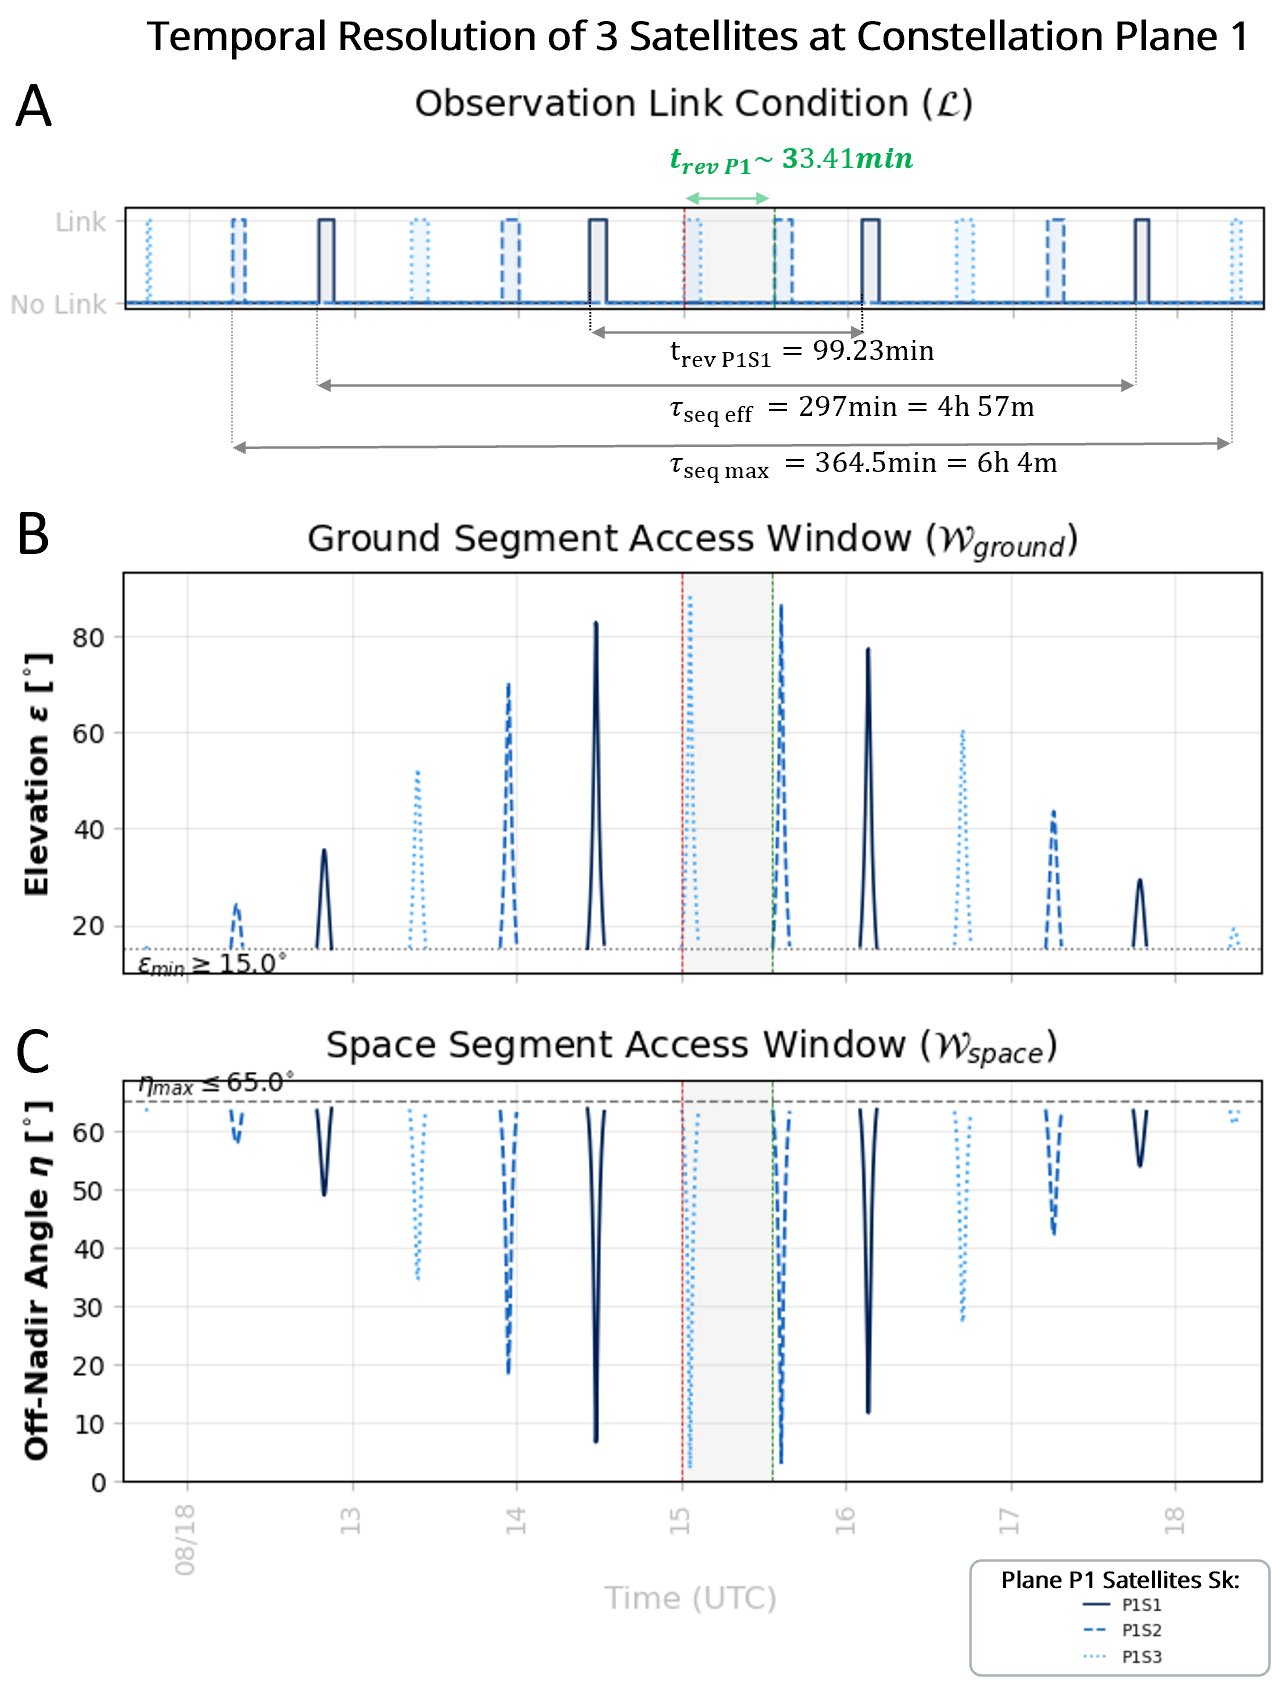
\includegraphics[width=1\linewidth]{images/temporal_resolution_observational_link_constellationP1S1.png}
    \caption{Observation-link analysis for Plane~1 with three co-planar satellites ($P_1S_1$--$P_1S_3$, $\Delta\nu = 120^{\circ}$) on the $\tau=15/1$ RGTO.  \textbf{(a)}~Combined observation-link condition.  \textbf{(b)}~Elevation profile ($t_{\mathrm{rev,P1}} \approx 33.4$\,min).  \textbf{(c)}~Off-nadir angle per pass.}
    \label{fig:temporal_res_P1S1}
\end{figure}

\begin{figure}
    \centering
    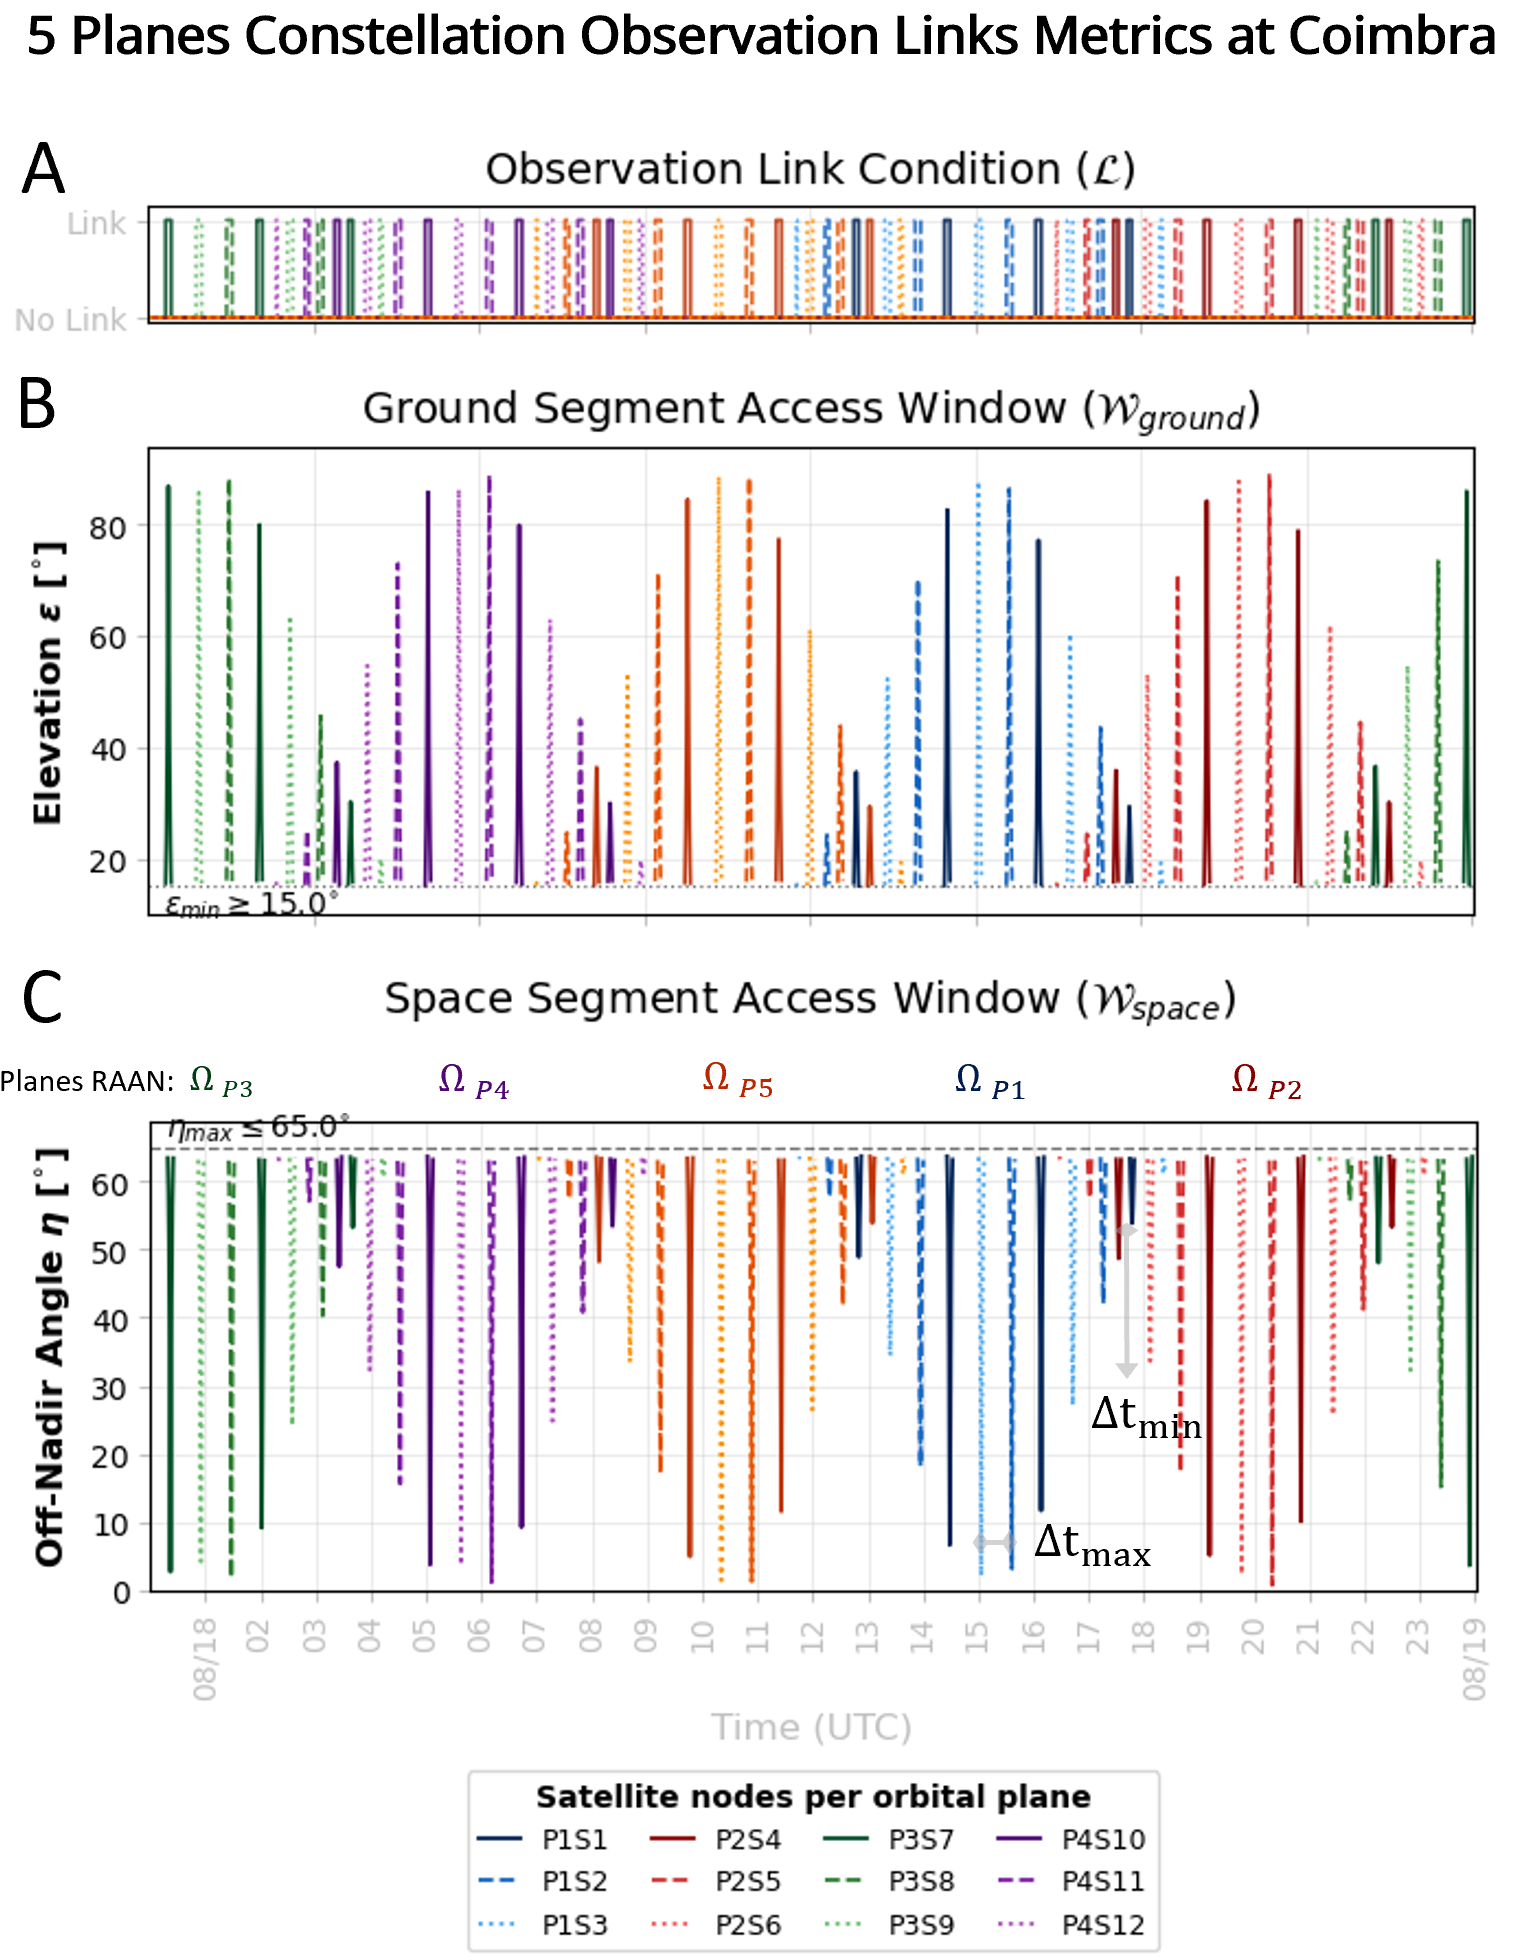
\includegraphics[width=1\linewidth]{images/5_planes_Constellation_Observation_Links_at_Coimbra.png}
    \caption{Observation links at Coimbra for the 5-plane Walker RGTO constellation $\mathcal{C}_{15/5/72}$ ($T_{\mathrm{seq,eff}} \approx 297$\,min, $\delta\Omega = 72^{\circ}$).  Each plane carries three satellites phased $120^{\circ}$ apart; the combined coverage spans the full day with $t_{\mathrm{rev}} \lesssim 33$\,min.}
    \label{fig:obs_links_5planes}
\end{figure}


\subsubsection{Conclusion: Baseline Constellation Parameters}
\label{sec:baseline_constellation_params}

The following parameters will be used in the next chapters to evaluate the performance of the baseline spacecraft cluster.
Table~\ref{tab:walker_c15} lists the RAAN and initial true anomaly for each of the 15~satellites in the baseline constellation $\mathcal{C}_{15/5/72}$.  All spacecraft share the RGTO seed orbit of Table~\ref{tab:rgto_parameters_coimbra} ($\tau=15/1$, $e=0.001$, $i=40.20329^{\circ}$, $\omega=0^{\circ}$), with $\Omega_{\mathrm{ref}}=100^{\circ}$ chosen to align $P_1S_1$ with the 18~August 15:00\,LT fire-peak pass over Coimbra.  This configuration, with $t_{\mathrm{rev}} \approx 33$\,min, is the closest Walker solution that satisfies the mission requirements $t_{\mathrm{rev}} \leq 30$\,min and GSD\,$< 6$\,m\,px$^{-1}$ throughout the full day over $\mathcal{D}_{\mathrm{core}}$, and is therefore adopted as the baseline constellation (\reqRef{R7}, \reqRef{R8}).

If sub-30-minute revisit is required, each plane can be further populated with four satellites phased $\Delta\nu = 90^{\circ}$, yielding $\mathcal{C}_{20/5/72}$ with $t_{\mathrm{rev}} \approx 25$\,min.  The full orbital-element tables for the baseline, the 4-plane candidate $\mathcal{C}_{12/4/90}$, and the high-cadence variant $\mathcal{C}_{20/5/72}$ are collected in Appendix~\ref{app:constellation_tables}, Table~\ref{tab:walker_constellations}.

\begin{table}[H]
\centering
\caption{\footnotesize{Baseline satellite parameter Walker RGTO constellation $\mathcal{C}_{15/5/72}$}}
\label{tab:walker_c15}
\smallskip
\footnotesize
\setlength{\tabcolsep}{4pt}
\begin{tabular}{c c r r}
\toprule
Plane & $S_k$ & $\Omega\;[^{\circ}]$ & $\nu_0\;[^{\circ}]$ \\
\midrule
\multirow{3}{*}{$P_1$} & $S_1$  & 100 &   0 \\
                        & $S_2$  & 100 & 120 \\
                        & $S_3$  & 100 & 240 \\
\midrule
\multirow{3}{*}{$P_2$} & $S_4$  & 172 &   0 \\
                        & $S_5$  & 172 & 120 \\
                        & $S_6$  & 172 & 240 \\
\midrule
\multirow{3}{*}{$P_3$} & $S_7$  & 244 &   0 \\
                        & $S_8$  & 244 & 120 \\
                        & $S_9$  & 244 & 240 \\
\midrule
\multirow{3}{*}{$P_4$} & $S_{10}$ & 316 &   0 \\
                        & $S_{11}$ & 316 & 120 \\
                        & $S_{12}$ & 316 & 240 \\
\midrule
\multirow{3}{*}{$P_5$} & $S_{13}$ &  28 &   0 \\
                        & $S_{14}$ &  28 & 120 \\
                        & $S_{15}$ &  28 & 240 \\
\bottomrule
\end{tabular}
\end{table}


% --- Part III: RESULTS, DISCUSSION, AND CONCLUSION ---
% ----------------------------------------
\part{\texorpdfstring{\textbf{RESULTS, DISCUSSION, AND
CONCLUSION}}{PART III: RESULTS, DISCUSSION, AND CONCLUSION}}
\label{part-iii-results-discussion-and-conclusion}

% --- Chapter 9: The Proposed System Concept ---
\chapter{The Proposed System
Concept}\label{chapter-9-the-proposed-system-concept}

The preceding chapters established the wildfire monitoring challenge and the observation requirements that a dedicated satellite system must satisfy.  Chapter~\ref{chapter-2-the-wildfire-challenge-and-study-case-definition-from-global-threat-to-local-data-needs} characterised the spatio-temporal dynamics of wildfires across fire-prone regions, Chapter~\ref{chapter-3-the-physics-of-wildfire-remote-sensing} defined the physics of fire remote sensing that constrains instrument design, and Chapter~\ref{chapter-2-the-wildfire-challenge-and-study-case-definition-from-global-threat-to-local-data-needs} formalised the mission requirements,in particular the temporal resolution target $\Delta t \lesssim 30$\,min (\reqRef{R7}), the spatial resolution target $\Delta s \lesssim 10$\,m/pixel (\reqRef{R8}), and the continuous coverage of the core study domain~$\mathcal{D}_{\text{core}}$ (\reqRef{R10}).  Chapter~\ref{73-constellation-design-architectures} translated these requirements into candidate constellation architectures through a systematic design-space exploration, producing the Walker-delta RGTO baseline $\mathcal{C}_{15/5/72}$ (15~satellites, 5~orbital planes, 3~satellites per plane) as the selected Low Earth Orbit constellation layer.

This chapter synthesises those results into a complete system concept.  The baseline constellation $\mathcal{C}_{15/5/72}$ is first formally introduced as the Zoom layer and its orbital parameters are recalled (Section~\ref{sec:detailed_constellation_orbital_parameters}).  The central questions that follow are: \emph{how does this constellation perform over the global domain and over the Portuguese core domain?  What sensor configuration minimises the total satellite count while still meeting the mission requirements?  And what architectural challenges emerge from the performance analysis that a single LEO layer alone cannot resolve?}

To answer these questions, Section~\ref{sec:zoom_layer} evaluates the constellation coverage through a parametric sweep of the sensor off-nadir angle~$\eta$, examining the trade-off between the effective observation envelope and the number of satellites required.  Section~\ref{sec:proposed_architecture} then addresses the architectural gap identified by this analysis by introducing a novel layered concept, designated the Watcher--Zoom ``tip-and-cue'' architecture, which combines the baseline LEO constellation with an existing geostationary fire-detection layer to achieve capabilities unattainable by either layer alone.  Finally, Section~\ref{sec:constellation_architecture_initial_demonstration} provides an initial demonstration of this concept, validating the coarse-to-fine observation chain with real active-fire data.


\section{Selected LEO Baseline Constellation Layer: $\mathcal{C}_{\text{Zoom}}$}
\label{sec:detailed_constellation_orbital_parameters}

The applied methodology produced a result that we selected as the mission baseline architecture: the Walker-delta RGTO constellation $\mathcal{C}_{15/5/72}$ (15~satellites, 5~planes, 3~satellites per plane), whose complete orbital parameters are given in Table~\ref{tab:walker_constellations}. This constellation $\mathcal{C}_{15/5/72}$ will be part of the layered architecture described in the following section \ref{sec:proposed_architecture}. From now on, we will refer to this Low Earth Orbit constellation layer as Zoom layer $\mathcal{C}_{\text{Zoom}}$. 
\begin{equation}
    \mathcal{C}_{\text{Zoom}} = \mathcal{C}_{15/5/72},
    \label{eq:zoom_layer_constellation}
\end{equation}
This configuration satisfies the mission's temporal and spatial resolution requirements,
 throughout the full day over the core study domain~$\mathcal{D}_{\mathrm{core}}$, \reqRef{R7}, \reqRef{R8}, \reqRef{R10}.

Figures~\ref{fig:GaiaFireeyes_Constellation3} illustrate the $\mathcal{C}_{\text{Zoom}}$ geometry in a 3D view and ground track plot. On this figure, we can observe the constellation setup of spacecrafts with conical sensors defined by the maximum geometrical observation-link access with off-nadir angle $\eta_{max} = 65^{\circ}$ as described by observation condition equation \ref{eq:observation_link_condition} and illustrated at Fig \ref{fig:access_window_configs}. As the sensor off-nadir access angle is a key enabler for achieving the required temporal resolution, the next sections analyze the performance of $\mathcal{C}_{\text{Zoom}}$ design in terms of coverage against $\eta$.



\begin{figure}[H]
    \centering
    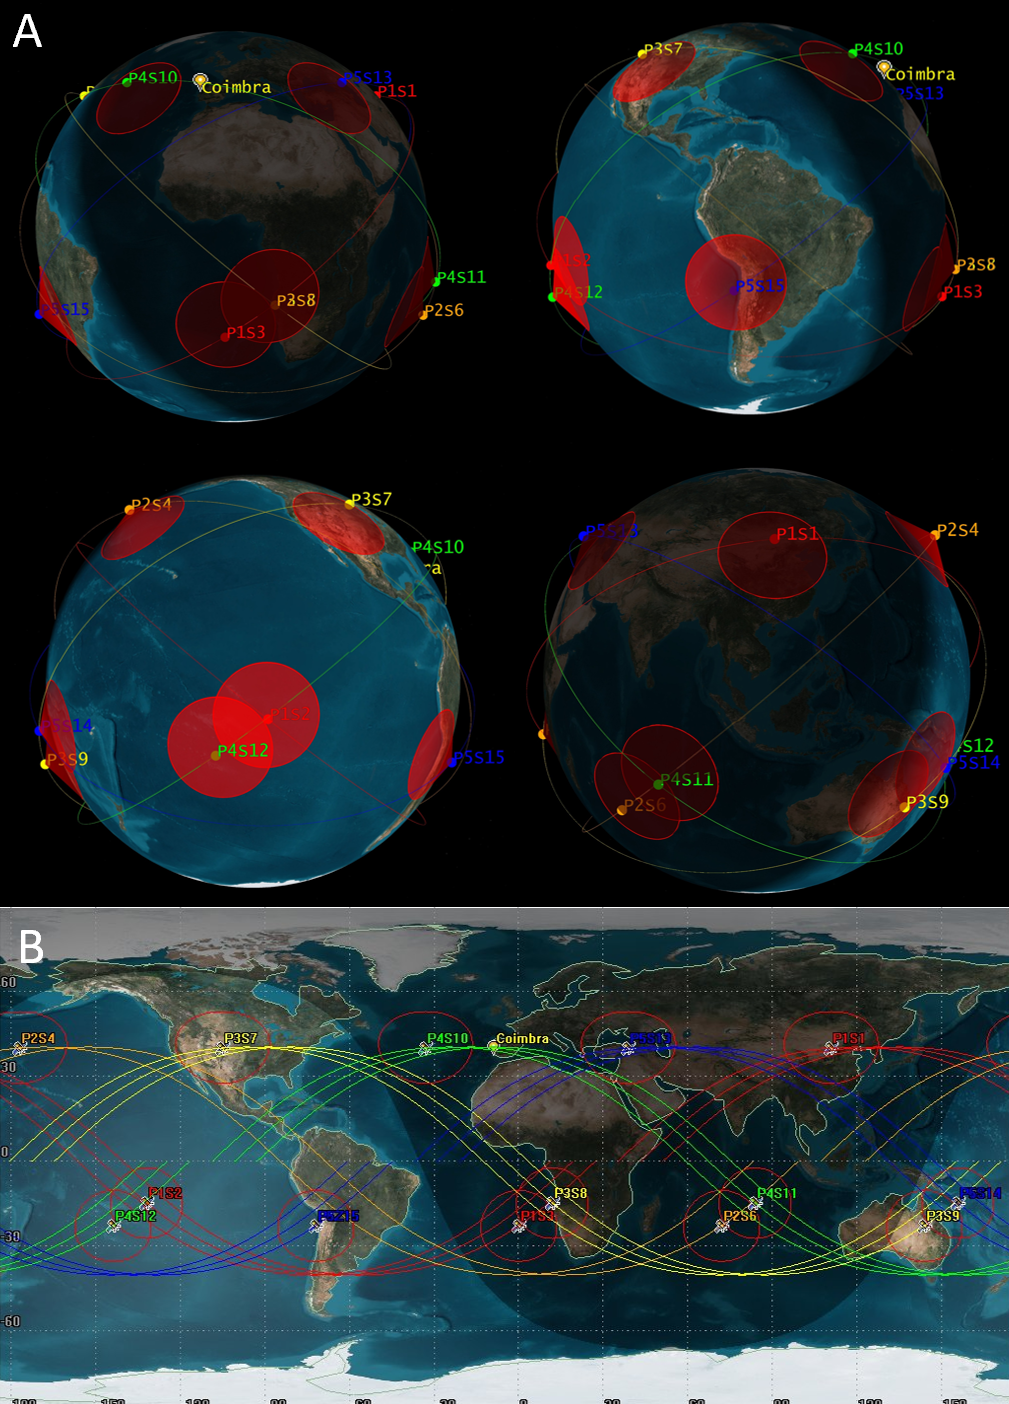
\includegraphics[width=0.92\linewidth]{images/GaiaFireeyes_Constellation3.png}
    \caption{\footnotesize{$\mathcal{C}_{\text{Zoom}} = \mathcal{C}_{15/5/72}$ constellation geometry. \textbf{(a)}~Four 3D views of the orbital configuration, showing the 15 satellites distributed across 5 planes (3 satellites per plane). \textbf{(b)}~Ground track plot over the global map. Each orbital plane is colour-coded: Plane~1 (P1)~-- red; Plane~2 (P2)~-- orange; Plane~3 (P3)~-- yellow; Plane~4 (P4)~-- green; Plane~5 (P5)~-- blue. The spacecraft conical sensor envelopes visible in the panels represent the maximum geometrical observation-link access at off-nadir angle $\eta_{\max} = 65^{\circ}$; they represent the space-segment access geometry.}}
    \label{fig:GaiaFireeyes_Constellation3}
\end{figure}




\section{Zoom Layer Results and Performance Analysis}
\label{sec:zoom_layer}

The goal of this section is to analyze the performance of the $\mathcal{C}_{\text{Zoom}}$ constellation if the sensor effective field of view $\eta$ is a variable. We want to define a set of $\eta$ values to explore this metrics results. 

As described in Section~\ref{sec:constellation_plane1}, the temporal resolution of the constellation $t_{\text{revisit}}$ is determined by the number of spacecrafts per plane $N_{\text{s/P}} = 3$. To achieve a full day coverage, this same setting of spacecraft need to be copied into new planes sharing the same origin but with a Right Ascension of the Ascending Node (RAAN) phase angle $\Omega$ between the planes. The number of orbital planes $P$ required to maintain $t_{\text{revisit}} \approx 30$\,min for a full day, is set by the effective observation-link sequence time $\tau_{\text{seq,eff}}$, i.e.\ the duration off the pass sequences of the 3 coplanar satellites over the core domain $\mathcal{D}_{\text{core}}$. Given a full day $t_{\text{day}} = 1440$\,min, the minimum plane P count is:
\begin{equation}
    P = \frac{t_{\text{day}}}{\tau_{\text{seq,eff}}}
    \label{eq:planes_from_tau}
\end{equation}
The total satellite count follows as $T = P \times N_{\text{s/P}}$, with $N_{\text{s/P}} = 3$ fixed throughout. Because $\tau_{\text{seq,eff}}$ decreases with the maximum allowed off-nadir angle $\eta$, a sensor restricted to small $\eta$ values forces a proportionally larger constellation. Table~\ref{tab:zoom_layer_configurations} and Figure~\ref{fig:observation_link_VS_eta_trade_off} quantify this trade-off across four representative configurations. Configuration ~\# c1 ($\eta = 65^{\circ}$) yields the minimum viable constellation of $T = 15$ satellites and is the selected $\mathcal{C}_{\text{Zoom}}$ baseline, conditional on a sensor with sufficient effective FOV (via tactical pointing or scanning) to exploit $\eta_{\max} \approx 65^{\circ}$.

\begin{table}[H]
    \centering
    \caption{\footnotesize{Off-nadir angle $\eta$ vs.\ constellation size trade-off (Eq.~\ref{eq:planes_from_tau}, $t_{\text{day}} = 1440$\,min, $N_{\text{s/P}} = 3$). Baseline configuration highlighted.}}
    \label{tab:zoom_layer_configurations}
    \small
    \begin{tabular}{cccccc}
        \toprule
        \textbf{c\#} & 
        \textbf{Off-Nadir $\boldsymbol{\eta}$ [\textdegree]} & 
        \textbf{$\boldsymbol{\tau_{\text{seq,eff}}}$ [min]} & 
        \textbf{$\boldsymbol{P}$ [planes]} & 
        \textbf{Sat/P} &
        \textbf{Total Sats $\boldsymbol{T}$} \\
        \midrule
        \rowcolor{green!15}
        1 & $65$ & $297.0$  & $5$  & $3$ & $\mathbf{15}$ \\
        2 & $45$          & $238.4$  & $7$  & $3$ & $21$          \\
        3 & $30$          & $172.41$ & $9$  & $3$ & $27$          \\
        4 & $15$          & $106.7$  & $14$ & $3$ & $\mathbf{42}$ \\
        \bottomrule
    \end{tabular}
    \label{tab:Czoom_eta_configurations}
\end{table}

The $\mathcal{C}_{\text{Zoom}}$ is subsequently analyzed for the metrics: Average Pass Duration; Number of Pass; Temporal Coverage. These performances are evaluated over the global domain $\mathcal{D}_{\text{global}}$ against fire-prone regions~(FPR) grouped by recurrence: recurrent ($r$, ${>}7$ fires/decade), occasional ($o$, ${<}3$), and infrequent ($i$, ${<}1$). The following subsections focus on the highest-priority recurrent group~$\mathrm{FPR}_{r}$.

\begin{figure}[H]
    \centering
    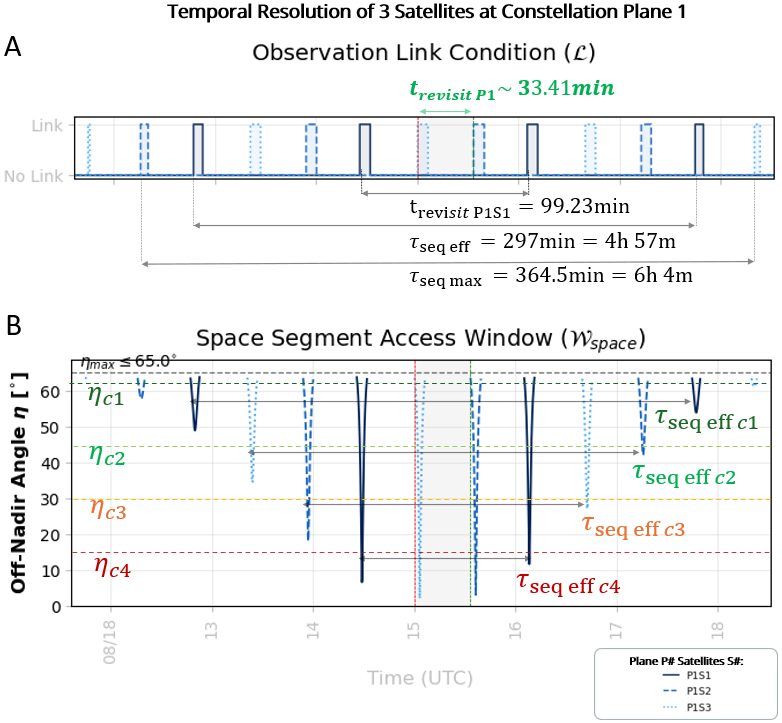
\includegraphics[width=0.82\linewidth]{images/observation_link_VS_eta_trade_off.png}
    \caption{\footnotesize{Zoom layer sensor trade-off analysis. (A) Observation link condition and temporal resolution analysis for a single plane. (B) Space segment access window ($\mathcal{W}_{\text{space}}$) as a function of off-nadir angle $\eta$. A wider allowable angle (e.g., $\eta_{c1}$) yields a longer effective sequence $\tau_{\text{seq, eff}}$, reducing the number of planes needed.}}
    \label{fig:observation_link_VS_eta_trade_off}
\end{figure}


%%% ================================================================
%%% Phase 1 — Performance Metrics Definition
%%% ================================================================
\subsection{Performance Metrics Definition}
\label{sec:performance_metrics_definition}

Before presenting the simulation results, this subsection defines the performance metrics used throughout this analysis.  All quantities are evaluated over a single-day simulation window ($t_{\text{day}} = 1440$\,min) and are computed per ground-grid points $P_j$ (120x360 grid cells) unless otherwise noted.

\begin{enumerate}
    \item \textbf{Off-nadir angle} ($\eta$): the angle between the satellite nadir direction and the line of sight to a ground  defined at equation \ref{eq:eta} and with values cited in Figure \ref{fig:observation_link_VS_eta_trade_off}

    \item \textbf{Number of passes} ($N_{\text{pass}}$): the total count of individual satellite passes per day over a given ground point $P_j$, where a pass is an uninterrupted interval during which the observation-link condition (Eq.~\ref{eq:observation_link_condition}) is satisfied.

    \item \textbf{Average pass duration} ($\bar{t}_{\text{pass}}$): the mean duration of a single pass over $P_j$, in minutes. It represents the mean imaging dwell time available to the payload per overpass event.

    \item \textbf{Temporal coverage} ($T_{\text{cov}}$): the cumulative time (hours per day) during which spacecrafts of the constellation satisfies the observation-link condition over a ground point $P_j$.
    \item \textbf{Minimum revisit time} ($\Delta t_{\min}$): the shortest gap between two consecutive passes over a ground point $P_j$, typically arising from the overlap between the last satellites of one orbital plane sequence and the first satellites of the next (see Fig.~\ref{fig:obs_links_5planes} for a visual example at Coimbra).

    \item \textbf{Maximum revisit time} ($\Delta t_{\max}$): the longest gap between consecutive passes over $P_j$. For the $\mathcal{C}_{\text{Zoom}}$ baseline design, this value is driven by the inter-plane RAAN spacing and the design target of $\Delta t_{\max} = t_{\text{revisit}} \approx 30$\,min.

    \item \textbf{Average revisit time} ($\Delta t_{\text{avg}}$): the mean temporal gap between consecutive passes over $P_j$, averaged over all gaps in the day.
\end{enumerate}

The analysis proceeds in four stages.  First, the global-domain maps of geometric and pass metrics ($\eta$, $N_{\text{pass}}$, $\bar{t}_{\text{pass}}$) are presented to characterize the observation geometry quality of the constellation (Section~\ref{sec:global_geometric_pass_metrics}).  Second, the temporal revisit metrics ($\Delta t_{\min}$, $\Delta t_{\text{avg}}$, $\Delta t_{\max}$) are mapped over $\mathcal{D}_{\text{global}}$ (Section~\ref{sec:global_temporal_metrics_Vs_eta}).  Third, the temporal coverage $T_{\text{cov}}$ is analyzed globally and then filtered through fire-prone region masks (Section~\ref{sec:global_Domain_temporal_coverage_Vs_eta}).  Finally, the metrics are extracted at the latitude of the core domain $\mathcal{D}_{\text{core}}$ to quantify the constellation performance over Portugal (Section~\ref{sec:portugal_core_domain_metrics_derive_from_global_domain_results}).


%%% ================================================================
%%% Phase 2 — Global Domain Geometric and Pass Metrics
%%% ================================================================
\subsection{Global Domain Geometric and Pass Metrics}
\label{sec:global_geometric_pass_metrics}

Figures~\ref{fig:c_zoom_avg_off_nadir}--\ref{fig:C_zoom_global_average_pass} map the three geometric and pass metrics $(\bar{\eta}$, $N_{\text{pass}}$, and $\bar{t}_{\text{pass}})$ over $\mathcal{D}_{\text{global}}$ for the four $\eta$ configurations of Table~\ref{tab:zoom_layer_configurations}.

The average off-nadir angle map (Fig.~\ref{fig:c_zoom_avg_off_nadir}) reveals that the latitude band $\phi \approx \pm\,40^{\circ}$ have the lowest $\bar{\eta} \approx 50^{\circ}$, meaning that satellites overpass this region closest to the nadir direction of the local grid points~$P_j(\phi \approx \pm\,40^{\circ})$.  This is a direct consequence of the RGTO inclination ($i = 40.02^{\circ}$): the ground-track density peaks near the orbital turning latitudes, concentrating low effective field of view passes over this band.  Outside $\phi \approx \pm\,40^{\circ}$, $\bar{\eta}$ rises to a near-uniform plateau of $\sim\!54$--$55^{\circ}$ across the remaining latitudes.  Crucially, the $\phi \approx 40^{\circ}$\,N belt coincides with both the core domain~$\mathcal{D}_{\text{core}}$ and the temperate-forest recurrent fire-prone regions (Fig.~\ref{fig:c_zoom_global_FRP_recurrent_ocasional_Tcoverage_eta63}), confirming that the orbit design concentrates the best observation geometry over the regions of highest mission priority.

The number-of-passes map (Fig.~\ref{fig:C_zoom_global_number_passes}) shows that the latitude of maximum $N_{\text{pass}}$ is displaced slightly equator-ward from $\phi = \pm\,40^{\circ}$, peaking near $\phi \approx \pm\,30^{\circ}$.  This offset arises because sub-satellite tracks from adjacent orbital planes converge and overlap at latitudes below the turning point, compounding the pass count.  The $\phi \approx \pm\,30^{\circ}$ overlap band may represent a favourable communication intercept latitude for a future inter-layer relay link between the Zoom layer and a communication layer $\mathcal{C}_{\text{Comm}}$, \inlineReq{R36}.

Finally, the average pass duration map (Fig.~\ref{fig:C_zoom_global_average_pass}) mirrors the $\bar{\eta}$ pattern: $\bar{t}_{\text{pass}}$ reaches its maximum of $\sim\!6$\,min at $\phi \approx \pm\,40^{\circ}$, where the near-nadir geometry prolongs each overpass, while the global background settles at $\sim\!5$\,min.  Together, the low $\bar{\eta}$ and high $\bar{t}_{\text{pass}}$ at the core-domain latitude confirm that $\mathcal{C}_{\text{Zoom}}$ delivers both the best image quality and the longest dwell time over $\mathcal{D}_{\text{core}}$. A result that will be corroborated by the global Fire Prone Regions coverage statistics in Section~\ref{sec:global_Domain_fire_prone_regions_statistics}.

\begin{figure}[H]
    \centering
    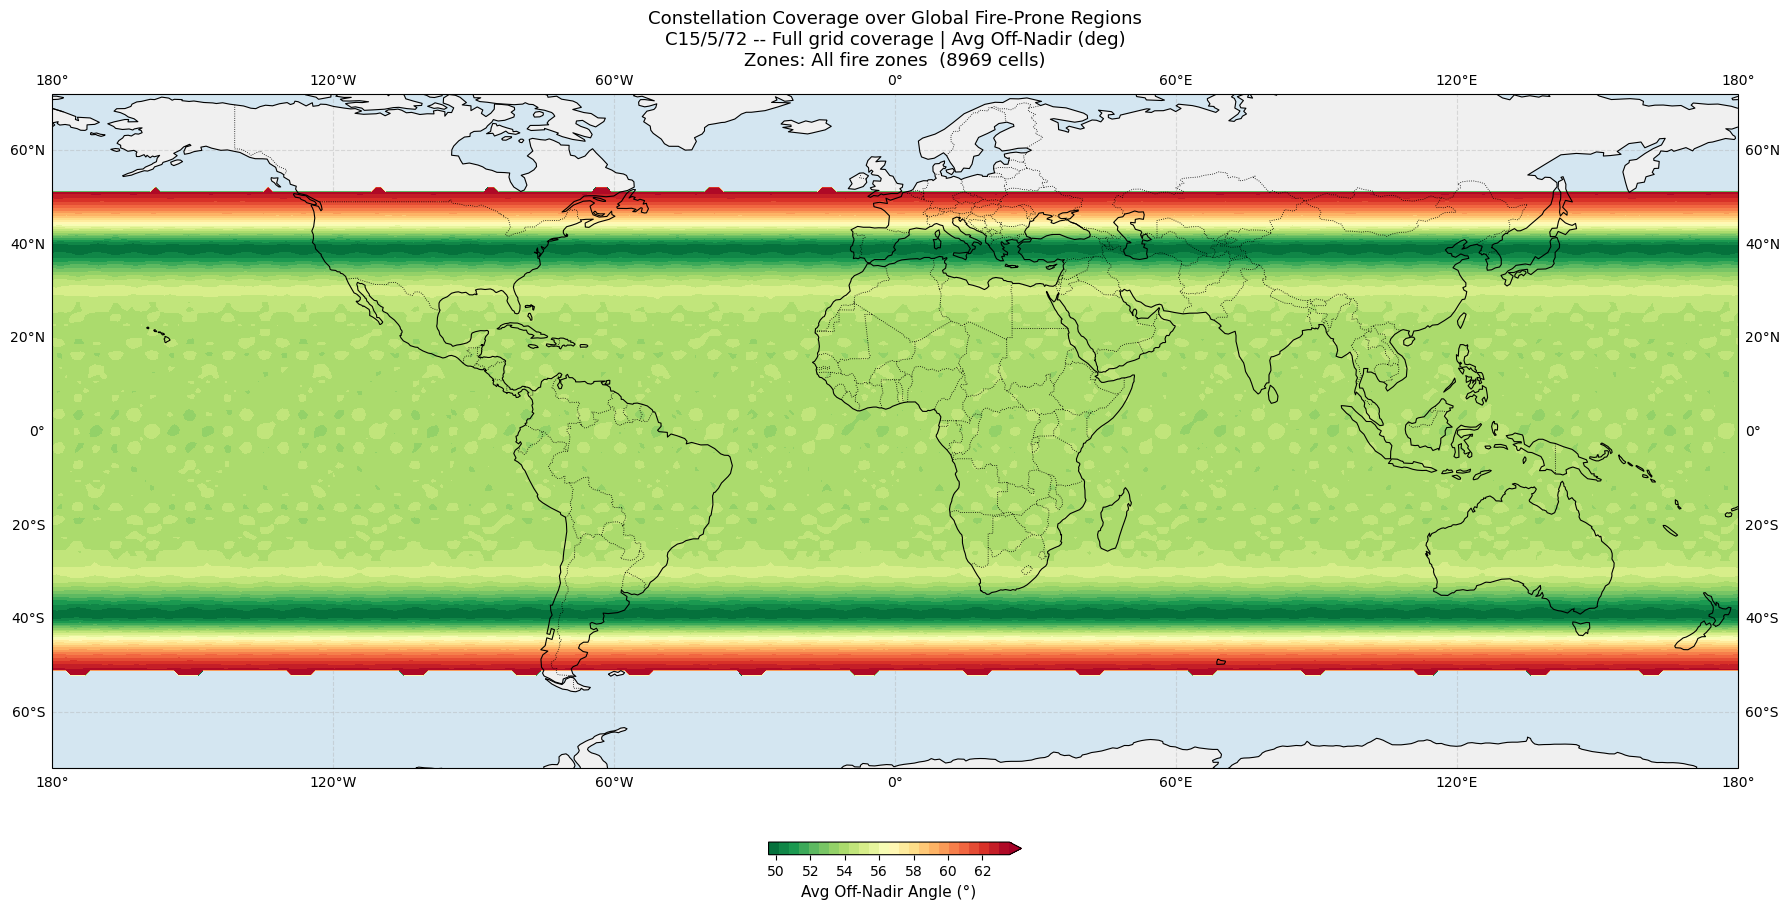
\includegraphics[width=1\linewidth]{images/c_zoom_avg_off_nadir.png}
    \caption{\footnotesize{Global map of the average off-nadir angle~$\bar{\eta}$ for $\mathcal{C}_{\text{Zoom}}$ across the four $\eta$ configurations (Table~\ref{tab:zoom_layer_configurations}).  The minimum $\bar{\eta} \approx 50^{\circ}$ occurs at latitudes $\phi \approx \pm\,40^{\circ}$, coinciding with $\mathcal{D}_{\text{core}}$ and the recurrent temperate Fire Prone Regions belt, while a near-uniform plateau of $\sim\!55^{\circ}$ covers the remaining latitudes.}}
    \label{fig:c_zoom_avg_off_nadir}
\end{figure}

\begin{figure}[H]
    \centering
    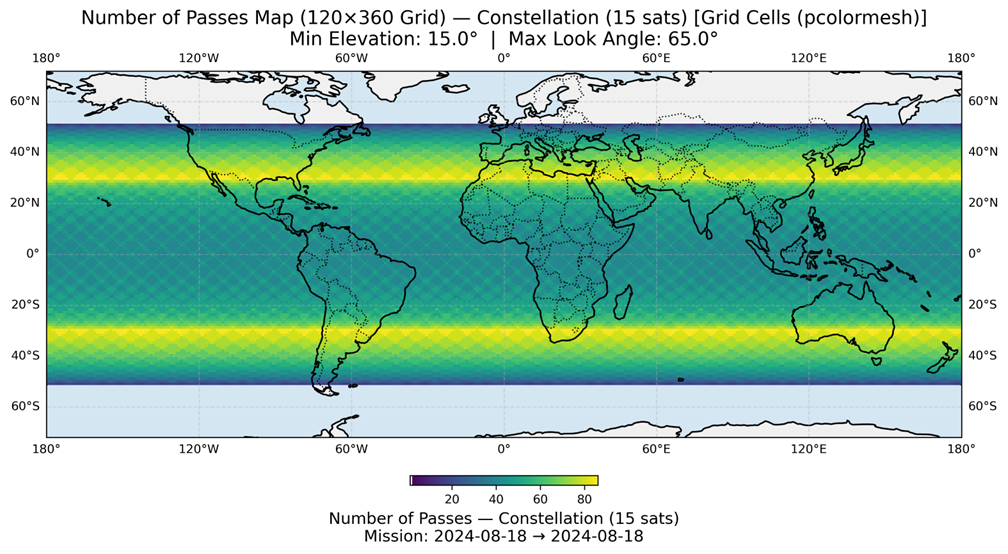
\includegraphics[width=1\linewidth]{images/C_zoom_global_number_passes.png}
    \caption{\footnotesize{Global map of the number of passes per day~$N_{\text{pass}}$ for $\mathcal{C}_{\text{Zoom}}$.  The maximum $N_{\text{pass} = 80}$ peaks near $\phi \approx \pm\,30^{\circ}$ due to inter-plane ground-track overlap, slightly equator-ward of the optimal geometry latitude, creating an optimal communication region.}}
    \label{fig:C_zoom_global_number_passes}
\end{figure}

\begin{figure}[H]
    \centering
    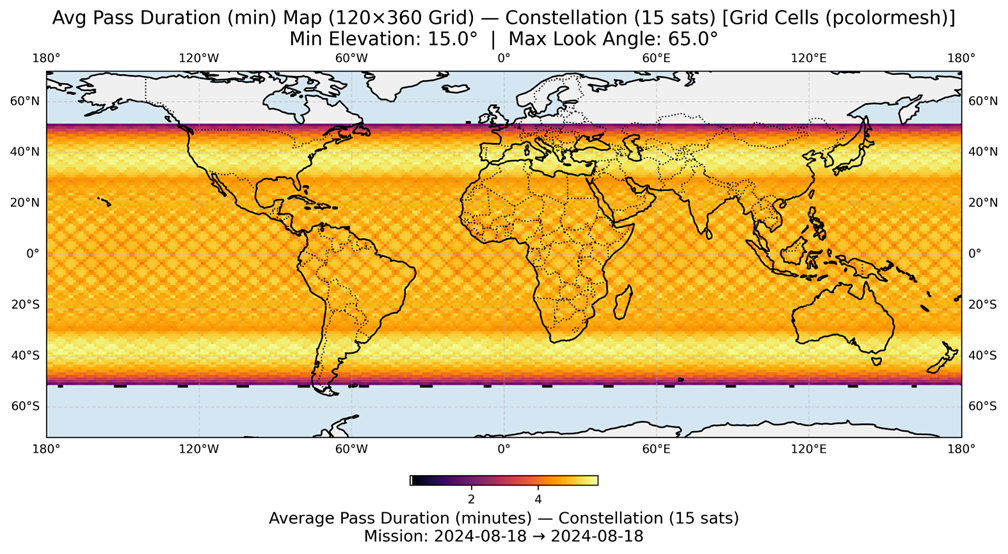
\includegraphics[width=1\linewidth]{images/C_zoom_global_average_pass.png}
    \caption{\footnotesize{Global map of the average pass duration~$\bar{t}_{\text{pass}}$ for $\mathcal{C}_{\text{Zoom}}$.  The maximum dwell of $\sim\!6$\,min is reached at $\phi \approx \pm\,40^{\circ}$ (RGTO resonance latitude), while the global average is $\sim\!5$\,min.}}
    \label{fig:C_zoom_global_average_pass}
\end{figure}


%%% ================================================================
%%% Phase 3 — Global Domain Temporal Metrics (Revisit)
%%% ================================================================
\subsection{Global Domain Temporal Metrics}
\label{sec:global_temporal_metrics_Vs_eta}

Figures~\ref{fig:c_zoom_min_revisit}--\ref{fig:c_zoom_max_revisit} map the three revisit metrics $(\Delta t_{\min}$, $\Delta t_{\text{avg}}$, and $\Delta t_{\max})$ over $\mathcal{D}_{\text{global}}$ for the baseline $\mathcal{C}_{\text{Zoom}}$ $\eta = 65^{\circ}$ configuration.

The minimum revisit map (Fig.~\ref{fig:c_zoom_min_revisit}) shows that the latitude band $\phi \approx \pm\,[25^{\circ}$--$45^{\circ}]$ achieves the most uniform $\Delta t_{\min} \approx 25$\,min, reflecting the dense plane-overlap geometry identified in Section~\ref{sec:global_geometric_pass_metrics}.  Gaps of higher $\Delta t_{\min}$ appear between $\phi \approx 0^{\circ}$--$20^{\circ}$, where the inter-plane phasing produces localized coverage holes of $\Delta t_{\min}$ 30min revisit surrounded by 10 min revisit regions.

The maximum revisit map (Fig.~\ref{fig:c_zoom_max_revisit}) confirms that across the same mid-latitude belt ($\phi \approx \pm\,[20^{\circ}$--$40^{\circ}]$) $\Delta t_{\max}$ remains close to the design target of $\sim\!30$\,min.  Near the equator, however, a gap band around $\phi \approx \pm\,15^{\circ}$ drives $\Delta t_{\max}$ up to $\sim\!115$\,min, corresponding to an period of the day with a temporal gap where no satellite satisfies the observation-link condition for approximately two hours.

The average revisit map (Fig.~\ref{fig:c_zoom_avg_revisit}) reaches its worst result at $\phi \approx \pm\,15^{\circ}$at with $\Delta t_{\text{avg}} \approx 50$\,min, and optimum values of $\Delta t_{\text{avg}} \approx 25$\,min near $\phi \approx \pm\,30^{\circ}$, the same pass-count peak latitude at Figure \ref{fig:C_zoom_global_number_passes}.  However, as established in Section~\ref{sec:global_geometric_pass_metrics}, this latitude does not coincide with the best observation geometry ($\bar{\eta}$ minimum at $\phi \approx \pm\,40^{\circ}$), making it more suited to a communication relay function than to high-resolution imaging.  At the core-domain latitude ($\phi \approx 40^{\circ}$\,N), $\Delta t_{\text{avg}} \approx 30$\,min, matching the mission design requirement $t_{\text{revisit}} \approx 30$\,min and confirming that $\mathcal{C}_{\text{Zoom}}$ delivers the specified monitoring cadence over Portugal $\mathcal{D}_{\text{Core}}$the recurrent temperate fire-prone regions.

\begin{figure}[H]
    \centering
    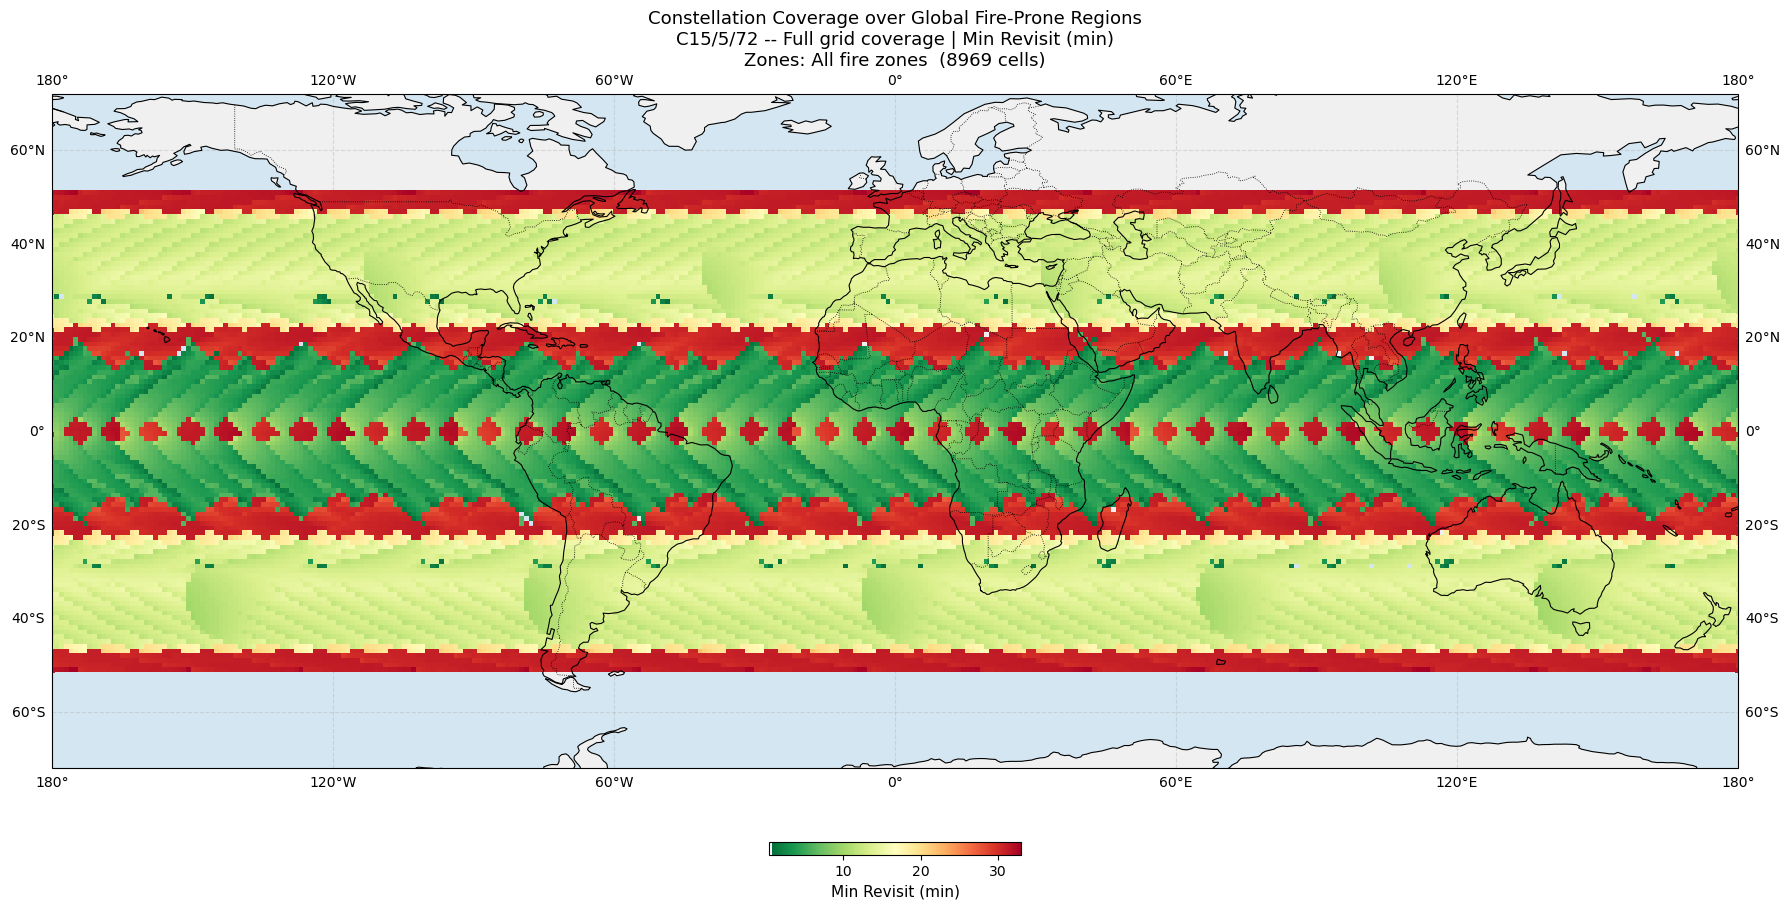
\includegraphics[width=1\linewidth]{images/c_zoom_min_revisit.png}
    \caption{\footnotesize{Global map of the minimum revisit time~$\Delta t_{\min}$ for $\mathcal{C}_{\text{Zoom}}$ ($\eta = 65^{\circ}$).  The most uniform band ($\Delta t_{\min} \approx 25$\,min) spans $\phi \approx \pm\,25^{\circ}$--$45^{\circ}$; sporadic gaps near the equator reflect inter-plane phasing discontinuities.}}
    \label{fig:c_zoom_min_revisit}
\end{figure}

\begin{figure}[H]
    \centering
    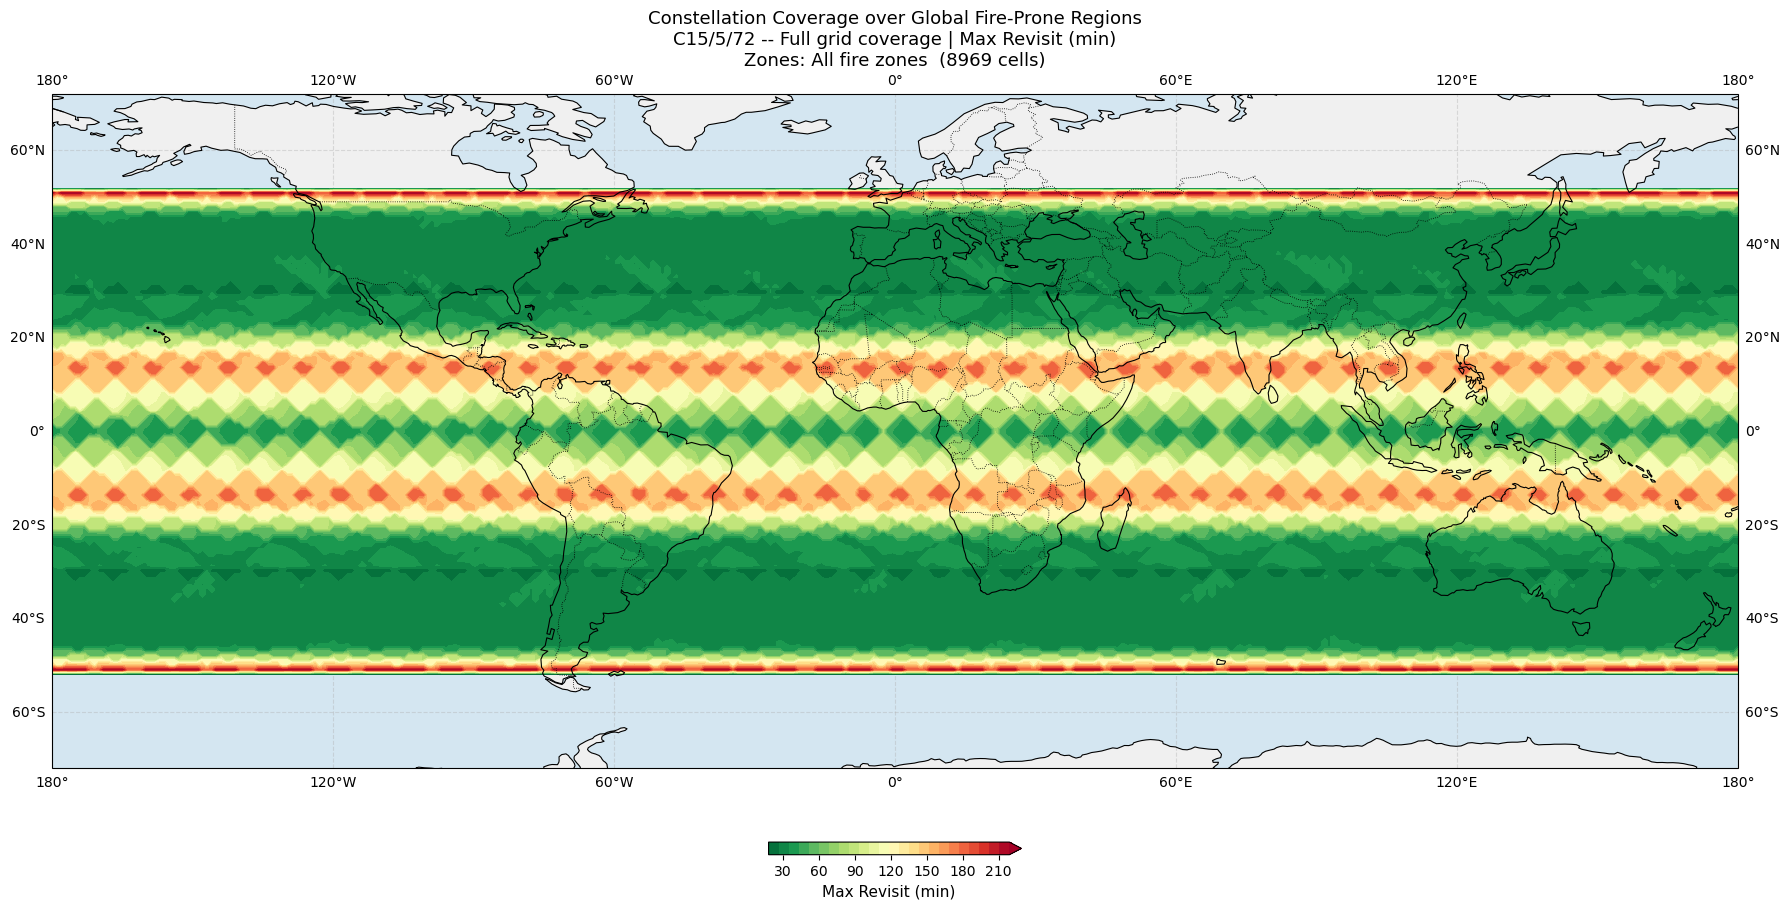
\includegraphics[width=1\linewidth]{images/c_zoom_max_revisit.png}
    \caption{\footnotesize{Global map of the maximum revisit time~$\Delta t_{\max}$ for $\mathcal{C}_{\text{Zoom}}$ ($\eta = 65^{\circ}$).  Mid-latitudes maintain $\Delta t_{\max} \approx 30$\,min; the worst-case gap of $\sim\!115$\,min appears near $\phi \approx \pm\,15^{\circ}$ due to an inter-plane RAAN discontinuity.}}
    \label{fig:c_zoom_max_revisit}
\end{figure}

\begin{figure}[H]
    \centering
    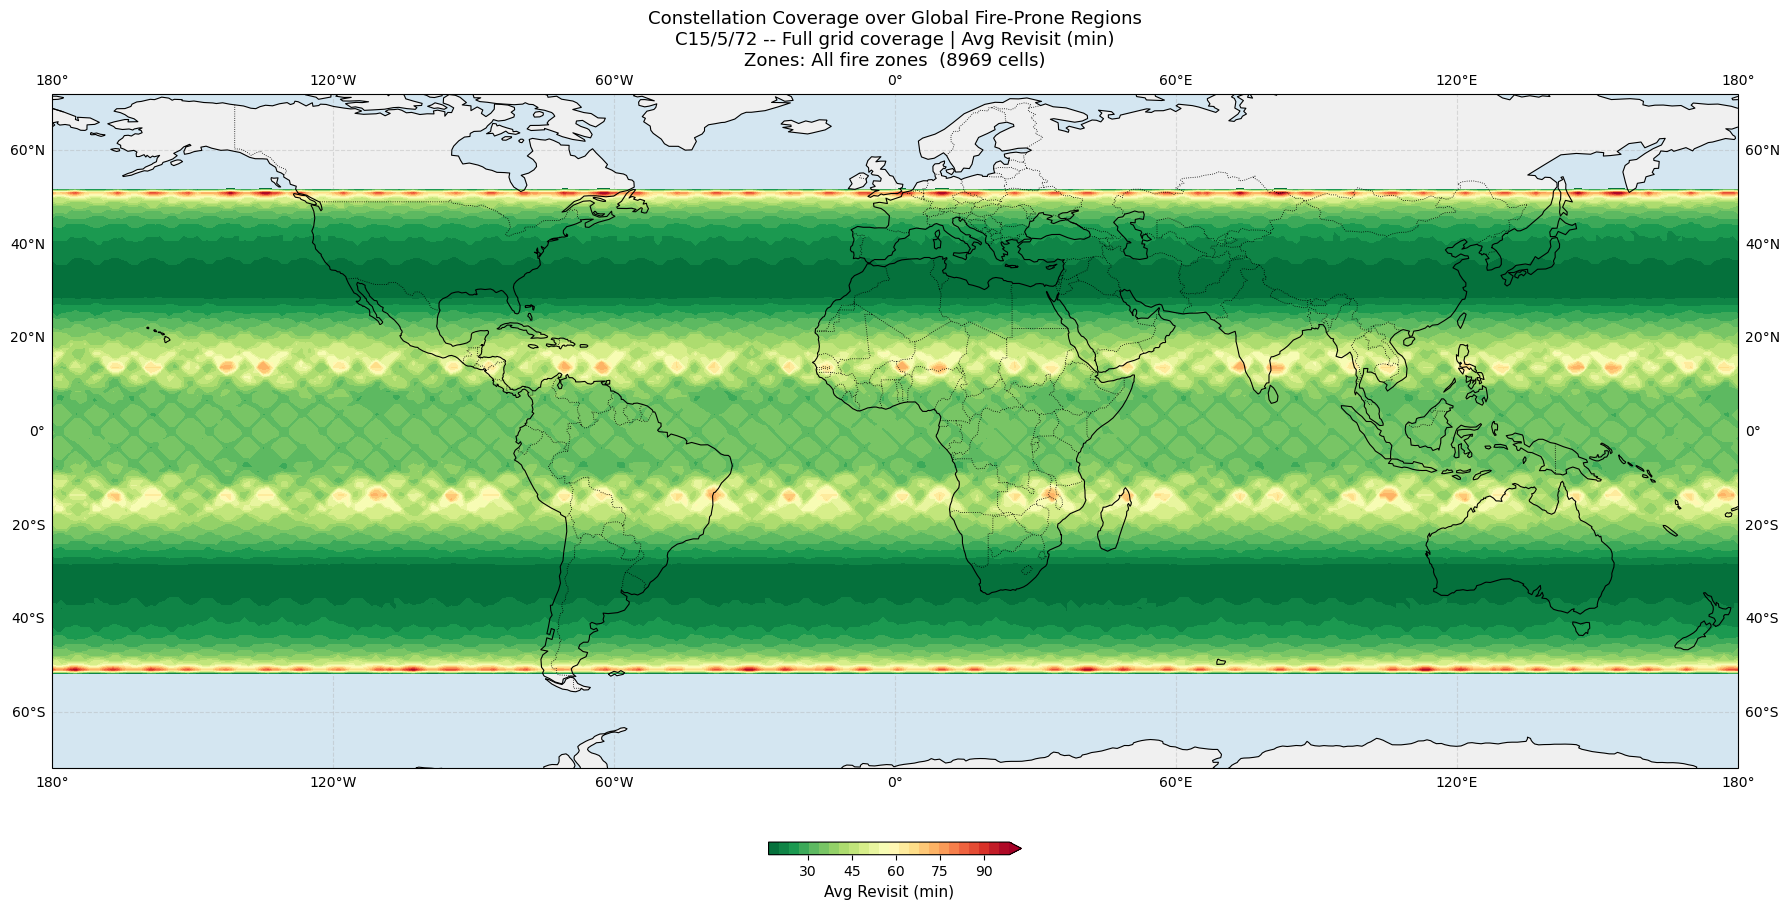
\includegraphics[width=1\linewidth]{images/c_zoom_avg_revisit.png}
    \caption{\footnotesize{Global map of the average revisit time~$\Delta t_{\text{avg}}$ for $\mathcal{C}_{\text{Zoom}}$ ($\eta = 65^{\circ}$).  The optimum $\Delta t_{\text{avg}} \approx 25$\,min occurs near $\phi \approx \pm\,30^{\circ}$ (pass-count peak); at the core-domain latitude $\Delta t_{\text{avg}} \approx 30$\,min, satisfying the design target.}}
    \label{fig:c_zoom_avg_revisit}
\end{figure}




%%% ================================================================
%%% Phase 4 — Global Temporal Coverage vs. Off-Nadir Angle
%%% ================================================================
\subsection{Global Domain Temporal Coverage Vs.\ Off-Nadir Angle}
\label{sec:global_Domain_temporal_coverage_Vs_eta}

Figure~\ref{fig:c_zoom_global_Tcovera_eta63} maps the temporal coverage~$T_{\text{cov}}$ over $\mathcal{D}_{\text{global}}$ for the baseline $\mathcal{C}_{\text{Zoom}}$ $\eta = 65^{\circ}$ configuration.  The latitude band $\phi \approx \pm\,30^{\circ}$ have the highest $T_{\text{cov}} \approx 7$\,h/day, a region suited for inter-layer communication relay already identified as the pass-count and revisit-time optimum (Sections~\ref{sec:global_geometric_pass_metrics}--\ref{sec:global_temporal_metrics_Vs_eta}).  At the core-domain latitude ($\phi \approx 40^{\circ}$\,N), $T_{\text{cov}} \approx 6$\,h/day; more broadly, the band $\phi \approx \pm\,[30^{\circ}$--$45^{\circ}]$ sustains $T_{\text{cov}} \approx 6$--$7$\,h/day, coinciding with the temperate fire-prone regions where high-cadence monitoring is most needed.  Equatorial latitudes ($|\phi| < 30^{\circ}$) reach $T_{\text{cov}} \approx 4$\,h/day, providing coverage for tropical fire-prone biomes.

The appendix maps (Figs.~\ref{fig:c_zoom_global_Tcoverage_eta45}--\ref{fig:c_zoom_global_Tcoverage_eta15}) illustrate the impact of reducing $\eta$.  At $\eta = 45^{\circ}$, the mid-latitude coverage contracts but still envelops $\mathcal{D}_{\text{core}}$; at $\eta = 30^{\circ}$, coverage fill Portugal area $\phi \approx 40^{\circ}$\,N; and at $\eta = 15^{\circ}$, only roughly half of Portugal remains within the coverage footprint.  Moreover, achieving full-day temporal resolution at lower $\eta$ demands a substantially larger constellation (e.g.\ $T = 27$ satellites in 9~planes for $\eta = 30^{\circ}$, Table~\ref{tab:zoom_layer_configurations}), increasing launch and orbital-insertion costs.  These results confirm that an effective off-nadir capability of $\eta \approx 65^{\circ}$ is a mission-critical requirement, to be addressed in future instrument-level studies through tactical pointing, scanning, or wide-swath sensor design,\inlineReq{R36}. 

\begin{figure}[H]
    \centering
    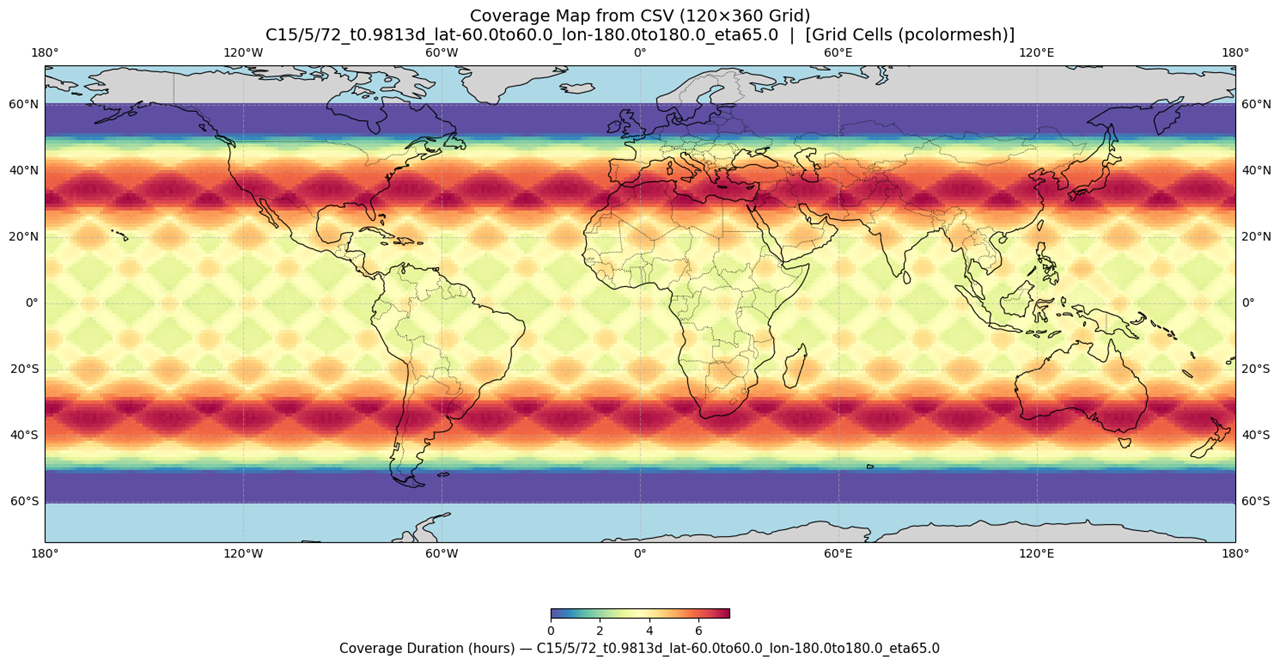
\includegraphics[width=1\linewidth]{images/c_zoom_global_Tcovera_eta63.png}
    \caption{\footnotesize{Global temporal coverage map~$T_{\text{cov}}$ for the $\mathcal{C}_{\text{Zoom}}$ baseline ($\eta = 65^{\circ}$).  Peak $T_{\text{cov}} \approx 7$\,h/day at $\phi \approx \pm\,30^{\circ}$; $T_{\text{cov}} \approx 6$\,h/day at the core-domain latitude;  coverage of ($\sim\!4$\,h/day) in equatorial regions.}}
    \label{fig:c_zoom_global_Tcovera_eta63}
\end{figure}

The corresponding temporal coverage maps for $\eta = 45^{\circ}$, $30^{\circ}$, and $15^{\circ}$ are provided in Appendix~\ref{appendix-figures} (Figs.~\ref{fig:c_zoom_global_Tcoverage_eta45}--\ref{fig:c_zoom_global_Tcoverage_eta15}).


%%% ================================================================
%%% Phase 5 — Fire-Prone Regions Coverage Analysis
%%% ================================================================
\subsection{Fire-Prone Regions Coverage Analysis}
\label{sec:fpr_coverage_analysis}

The preceding sections characterised the $\mathcal{C}_{\text{Zoom}}$ performance over the full global domain~$\mathcal{D}_{\text{global}}$.  To assess the constellation's effectiveness where it matters most, the temporal-coverage maps are now filtered through the fire-prone region (FPR) spatial masks derived from the wildfire recurrence classification introduced in Section~\ref{sec:earths_frp_targets}, represented in Figure \ref{fig:c_zoom_global_Tcoverage_FRP_groups_Spatial_Mask}.  Three recurrence groups are considered: \emph{recurrent} ($r$, $> 7 FPY$/decade), \emph{occasional} ($o$, $3 < FPY\text{/decade} \leq 7$), and \emph{infrequent} ($i$, $0 < FPY\text{/decade} \leq 3$).  Because the recurrent and occasional group concentrates the highest-priority wildfire monitoring targets, the analysis that follows focuses on the broadest operationally relevant mask for these regions grid points $P_j$.  All results correspond to the baseline $\eta = 65^{\circ}$ configuration; the off-nadir sweep maps ($\eta = 45^{\circ}$, $30^{\circ}$, $15^{\circ}$) for each FPR group are deferred to Appendix~\ref{appendix-figures}.



%%% 5a — FPR Spatial Masks

\begin{figure}[H]
    \centering
    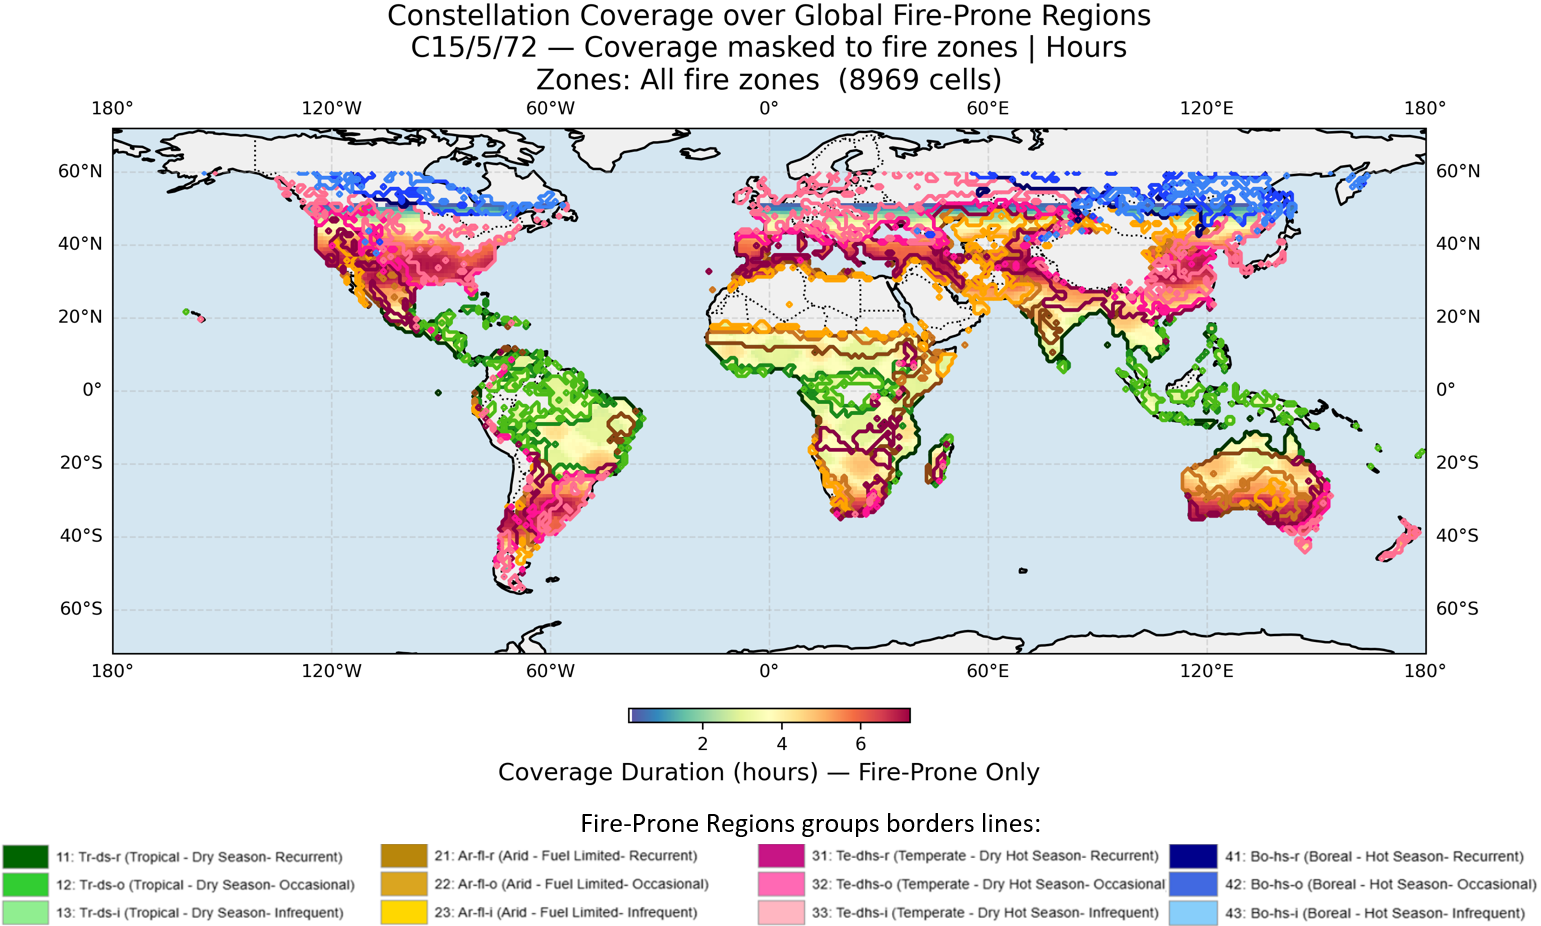
\includegraphics[width=1\linewidth]{images/c_zoom_global_Tcoverage_FRP_groups_Spatial_Mask.png}
    \caption{\footnotesize{Fire-prone region spatial masks overlaid on the $\mathcal{C}_{\text{Zoom}}$ temporal-coverage grid.  Each mask isolates the grid cells belonging to one FPR recurrence group---recurrent~($r$), occasional~($o$), and infrequent~($i$)---as classified in Section~\ref{sec:earths_frp_targets}.  The colour scale indicates $T_{\text{cov}}$ within each mask; non-FPR cells are greyed out.}}
    \label{fig:c_zoom_global_Tcoverage_FRP_groups_Spatial_Mask}
\end{figure}


%%% 5b — FPR Temporal Coverage at Baseline (η = 65°)
\subsubsection{Fire-Prone Region Temporal Coverage at Baseline ($\eta = 65^{\circ}$)}
\label{sec:fpr_temporal_coverage_baseline}

The FPR boundaries map (Fig.~\ref{fig:c_zoom_global_FRP_bondaries_Tcoverage_eta63}, Appendix~\ref{appendix-figures}) reproduces the latitude-dependent coverage pattern already identified in Section~\ref{sec:global_Domain_temporal_coverage_Vs_eta}: the highest $T_{\text{cov}}$ values concentrate at $\phi \approx \pm\,30^{\circ}$--$40^{\circ}$, coinciding with the pass-count and revisit-time optima of the constellation.  Filtering to the recurrent-only mask (Fig.~\ref{fig:c_zoom_global_FRP_recurrent_Tcoverage_eta63}, Appendix~\ref{appendix-figures}) isolates the temperate and Mediterranean forest biomes near $\phi \approx \pm\,40^{\circ}$, Tropical forests and Arid regions, confirming that constellation is optimized to the temperate biomes targets and also is great for the equatorial domains.

When the mask is broadened to include both recurrent \emph{and} occasional fire-prone regions (Fig.~\ref{fig:c_zoom_global_FRP_recurrent_ocasional_Tcoverage_eta63}), the coverage extent grows substantially: Amazonia, central Africa, south-eastern Australia, southern Africa, Chile, California, and boreal northern Europe all enter the monitored domain.  Within this combined mask, equatorial FPR zones maintain $T_{\text{cov}} > 3.5$\,h/day, while the mid-latitude temperate belt reaches $T_{\text{cov}} \approx 6$--$7$\,h/day---values consistent with the global baseline analysed in Section~\ref{sec:global_Domain_temporal_coverage_Vs_eta}.

Reading the combined FPR mask at country level reveals the breadth of the potential beneficiary nations.  In the \emph{temperate belt} ($\phi \approx \pm\,30^{\circ}$--$45^{\circ}$), where recurrent fire-prone regions concentrate and $T_{\text{cov}} \approx 5$--$7$\,h/day, the constellation covers:
\begin{itemize}[nosep]
    \item \textbf{North America}: the western and central United States (California, Oregon, Idaho, Utah, Colorado, Arizona, New~Mexico, Texas) and Mexico;
    \item \textbf{Southern Europe \& Mediterranean}: Portugal, Spain, Italy, Greece, Turkey, Morocco, Algeria, and Tunisia;
    \item \textbf{Near East \& Central Asia}: Syria, Lebanon, Iraq, Armenia, Azerbaijan, Iran, Afghanistan, Pakistan, and Uzbekistan;
    \item \textbf{South \& South-East Asia}: Nepal, northern India, Bangladesh, Myanmar, Thailand, Laos, and southern China;
    \item \textbf{Southern-hemisphere temperate}: southern Chile, Argentina, Paraguay, and Bolivia; South Africa and Madagascar; and southern and inland Australia.
\end{itemize}
In the \emph{equatorial belt} ($|\phi| < 30^{\circ}$), where $T_{\text{cov}} \approx 3$--$4$\,h/day, the constellation additionally services:
\begin{itemize}[nosep]
    \item \textbf{Caribbean \& Central America}: Cuba, Guatemala, and the remaining Central American nations;
    \item \textbf{South America}: Venezuela, the Brazilian Amazon basin, the Cerrado savanna, the Pantanal wetlands, and the semi-arid Nordeste region of Brazil;
    \item \textbf{Sub-Saharan Africa}: Africa being the most fire-active continent globally, have it's fire belt covered, including Nigeria, Congo, Angola, Mozambique, and Somalia, among others;
    \item \textbf{Maritime South-East Asia}: Indonesia and the Philippines.
\end{itemize}
Altogether, the $\mathcal{C}_{\text{Zoom}}$ constellation provides operationally useful temporal coverage to the vast majority of fire-prone nations worldwide.  The temperate-belt countries benefit from the highest $T_{\text{cov}}$ and the shortest revisit times, a direct consequence of the RGTO inclination placing the ground-track density peak at the latitudes of these regions. The equatorial nations, although receiving lower absolute $T_{\text{cov}}$, still obtain continuous daily monitoring that substantially exceeds the revisit cadence of current polar-orbiting fire-detection systems.

\begin{figure}[H]
    \centering
    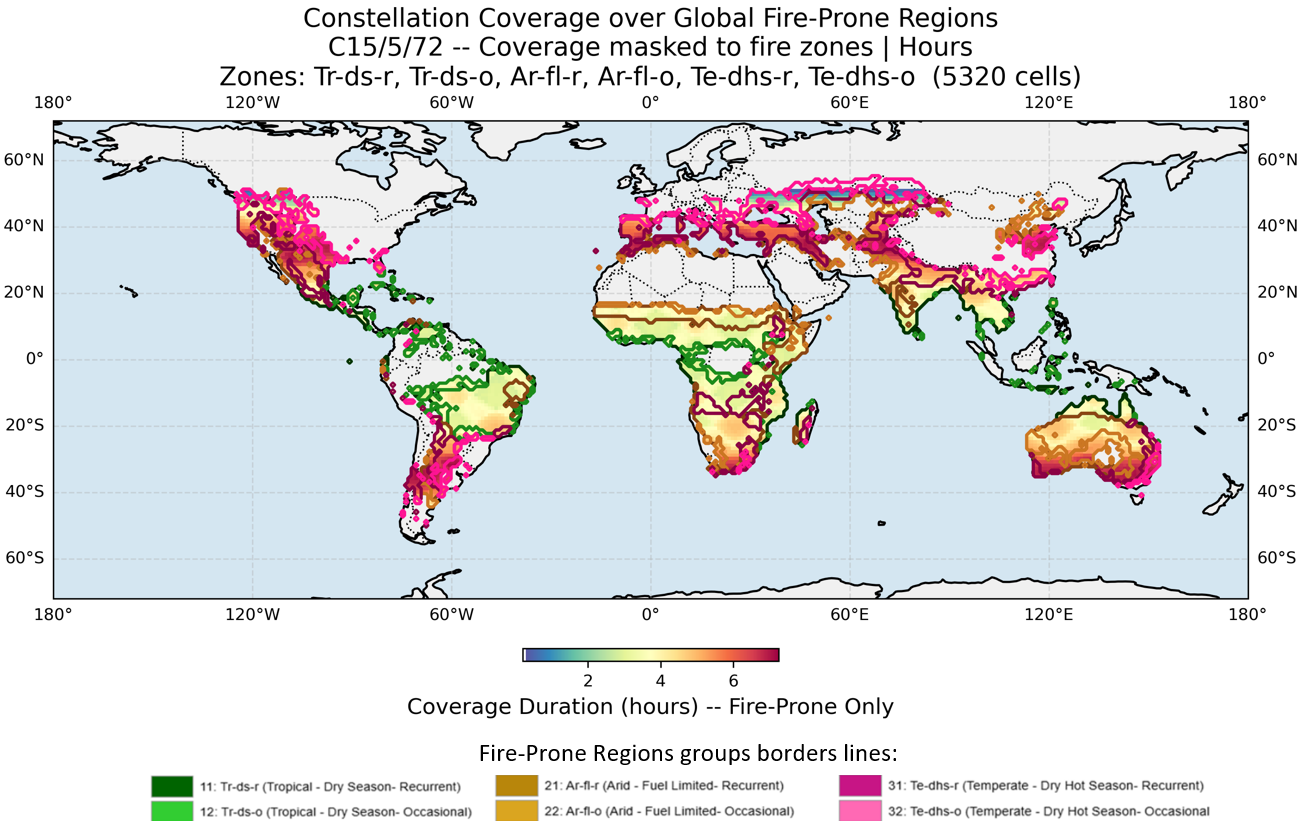
\includegraphics[width=1\linewidth]{images/c_zoom_global_FRP_recurrent_ocasional_Tcoverage_eta63.png}
    \caption{\footnotesize{Temporal coverage~$T_{\text{cov}}$ of the combined recurrent-and-occasional FPR mask for $\mathcal{C}_{\text{Zoom}}$ at the baseline $\eta = 65^{\circ}$.  The mask captures the operationally most relevant fire-prone regions worldwide; peak $T_{\text{cov}} \approx 6$--$7$\,h/day in the temperate belt ($\phi \approx \pm\,[30^{\circ}$--$45^{\circ}]$) and $T_{\text{cov}} > 3.5$\,h/day for other FPRs latitudes.  Boundaries-only and recurrent-only baseline maps are provided in Appendix~\ref{appendix-figures} (Figs.~\ref{fig:c_zoom_global_FRP_bondaries_Tcoverage_eta63}--\ref{fig:c_zoom_global_FRP_recurrent_Tcoverage_eta63}).}}
    \label{fig:c_zoom_global_FRP_recurrent_ocasional_Tcoverage_eta63}
\end{figure}


The temporal coverage maps for the remaining off-nadir configurations ($\eta = 45^{\circ}$, $30^{\circ}$, $15^{\circ}$) across all three FPR groups are provided in Appendix~\ref{appendix-figures}, Figs.~\ref{fig:c_zoom_global_FRP_boundaries_Tcoverage_eta45}--\ref{fig:c_zoom_global_FPR_recurrent_ocasional_Tcoverage_eta15}.


%%% 5c — FPR Coverage Statistics Summary
\subsubsection{Fire-Prone Region Coverage Statistics}
\label{sec:global_Domain_fire_prone_regions_statistics}

The bar-chart and scatter-plot breakdowns of the five performance variables across FPR groups and $\eta$ configurations are provided in Appendix~\ref{appendix-figures} (Figs.~\ref{fig:c_zoom_metrics_FPR_coverage_statistics}--\ref{fig:c_zoom_metrics_latitude_profile}).  Their results are consistent with the spatial maps above: the temperate-climate FPR group achieves the highest $T_{\text{cov}}$ and the shortest revisit times, while the constellation also operates over all other climate regions except boreal.  The latitude profile (Fig.~\ref{fig:c_zoom_metrics_latitude_profile}) is used in the following subsection to extract Portugal-specific metrics at $\phi = 40.02^{\circ}$\,N.

%%% ================================================================
%%% Phase 6 — Portugal Core Domain Performance
%%% ================================================================
\subsection{Portugal Core Domain Performance ($\mathcal{D}_{\text{core}}$)}
\label{sec:portugal_core_domain_metrics_derive_from_global_domain_results}

Reading the latitude profile (Fig.~\ref{fig:c_zoom_metrics_latitude_profile_not_norm} and Fig.~\ref{fig:c_zoom_metrics_latitude_profile}) at $\phi = 40.02^{\circ}$\,N at the constellation with baseline configuration ($\eta = 65^{\circ}$) generates the metrics for Portugal core-domain: \textbf{$T_{\text{cov}} \approx 6$\,h/day, $\bar{\eta} \approx 50^{\circ}$, $\Delta t_{\text{avg}} \approx 21$\,min, $\Delta t_{\max} \approx 34.67$\,min, and $\Delta t_{\min} \approx 12$\,min}.  These values satisfy the design targets \reqRef{R7}, \reqRef{R8}, \reqRef{R10}. The $t_{\mathrm{rev,P1}} \approx 33.41$ matches the inter-plane transit interval predicted in Section~\ref{sec:constellation_plane1}, while $\Delta t_{\min} \approx 12$\,min, arising from adjacent-plane overlap --- illustrated in Fig.~\ref{fig:obs_links_5planes},---  yields shorter revisit than originally anticipated from the single-plane design. \textbf{Leading to a better-than-expected average revisit time of $\Delta t_{\text{avg}} \approx 21$\,min, well below the design target of $t_{\text{revisit}} \approx 30$\,min.}  The $\bar{\eta} \approx 50^{\circ}$ at the core-domain latitude shown in Fig.~\ref{fig:c_zoom_avg_off_nadir} confirms that the constellation delivers the best observation geometry over Portugal, therefore, covering the full $\mathcal{D}_{\text{core}}$ defined in section \ref{sec_pt_space_domain}.

\subsection{Summary of Findings and Implications for the System Architecture}
\label{sec:zoom_layer_findings_summary}

The analysis presented in this section demonstrates that the $\mathcal{C}_{\text{Zoom}}$ constellation provides continuous temporal coverage over both the core domain~$\mathcal{D}_{\text{core}}$ and the global fire-prone regions, with revisit times that can reach sub-30-minute intervals not only over Portugal but across the temperate, tropical and arid FPR groups.  However, these performance levels are contingent on an effective sensor off-nadir capability of $\eta \approx 65^{\circ}$: the coverage maps and trade-off analysis (Table~\ref{tab:zoom_layer_configurations}) show that reducing $\eta$ rapidly degrades temporal resolution and demands a substantially larger constellation. Under constrained small satellite volumes, high spatial resolution sensor have narrow Field of View (FOV), exploiting the full geometric access envelope therefore requires the Zoom-layer instrument to be \emph{aimable}, capable of rapidly steering its FOV toward a designated target within the observation-link window.  This, in turn, implies a cueing mechanism that delivers timely fire-event information to the Zoom-layer spacecraft so that its sensor can be pointed in the correct direction before the access window closes.

A second finding emerges from the global pass-count and temporal-coverage maps (Figs.~\ref{fig:C_zoom_global_number_passes} and~\ref{fig:c_zoom_global_Tcovera_eta63}): the latitude band $\phi \approx \pm\,30^{\circ}$ concentrates the highest pass density and the peak $T_{\text{cov}}$, making it the geometrically optimal region for an inter-layer --- satellite-satellite or satellite-ground staiton ---  communication relay.  Taken together, these two results, the need for a cueing signal and the existence of a preferred relay latitude, define the functional requirements for a complementary constellation layer that can detect fire events at broad scale, relay the information to the Zoom layer, and enable targeted high-resolution observation.  The architecture that fulfils these requirements is proposed in the following section.


\section{Proposed Architecture: Watcher--Zoom ``Tip-and-Cue'' Concept}
\label{sec:proposed_architecture}

The preceding section established that $\mathcal{C}_{\text{Zoom}}$ can deliver sub-30-minute revisit with $\text{GSD} \approx 6$\,m/pixel over the core domain and global fire-prone regions, provided the sensor exploits an effective off-nadir envelope of $\eta \approx 65^{\circ}$.  Under small-satellite volume constraints, a high-spatial-resolution instrument has a narrow instantaneous FOV; therefore the Zoom-layer sensor must be \emph{aimable}, steered toward each fire target within the observation-link window.  This demands a cueing signal that arrives \emph{before} the access window closes.

In systems engineering, this cooperative multi-sensor strategy is known as a \emph{tip-and-cue} architecture (Fig.~\ref{fig:tip-and-cue_example}): each layer contributes a unique capability, one provides fast, coarse detection while the other delivers high-resolution confirmation.Their combination yields temporo-spatial fidelity unattainable by either layer alone~\cite{_architecture_tipcue}. 

Section~\ref{sec:geolayer_candidate_architecture} identified the existing geostationary fire-detection constellation composing the FIRMS dataset (Table~\ref{tab:geo_satellites}, Fig.~\ref{fig:firms_geostationary_sats}) as a candidate constellation $\mathcal{C}_{\text{Watcher}}$: five geostationary platforms (GOES-16/18, Meteosat-9/11, Himawari-8/9) that together cover Earth's full disk with a temporal resolution $\Delta t_{\text{Watcher}} \approx 10$--$15$\,min and a spatial resolution $\Delta s_{\text{Watcher}} \approx 2$--$3$\,km/pixel.

Figure~\ref{fig:watcher_zoom_3D_concept} illustrates the two-layer geometry: the geostationary $\mathcal{C}_{\text{Watcher}}$ layer provides continuous full-disk fire surveillance, while the LEO $\mathcal{C}_{\text{Zoom}}$ layer orbits beneath it.  The operational chain is detailed in Figure~\ref{fig:proposed_watcher_zoom_concept} and proceeds as follows.  A Watcher satellite $S_{\text{Watcher},i}$ detects fire activity and produces a coarse active-fire pixel (CAFPx) in its image $\mathcal{I}(S_{\text{Watcher},i})$, with $\Delta s_{\text{Watcher}} \approx 2$--$3$\,km/pixel and $\Delta t_{\text{Watcher}} \approx 10$--$15$\,min.  This detection is downlinked to a ground station via communication link~$\mathcal{L}_1$.  The ground segment relays the fire-alert message through link~$\mathcal{L}_2$ to a communication layer $\mathcal{C}_{\text{Comm}}$ (to be defined), which in turn transmits the cueing command via link~$\mathcal{L}_3$ to the Zoom-layer satellite $S_{\text{Zoom},k}$.  Upon reception, $S_{\text{Zoom},k}$ steers its dynamic boresight $\mathbf{b}_{k,\text{dynamic}}$ toward the CAFPx coordinates and acquires the fine active-fire pixel (FAFPx) image $\mathcal{I}(S_{\text{Zoom},k})$, with $\Delta s_{\text{Zoom}} \approx 6$\,m/pixel and $\Delta t_{\text{Zoom}} \lesssim 30$\,min (12--33\,min depending on inter-plane phasing).

\begin{figure}[H]
    \centering
    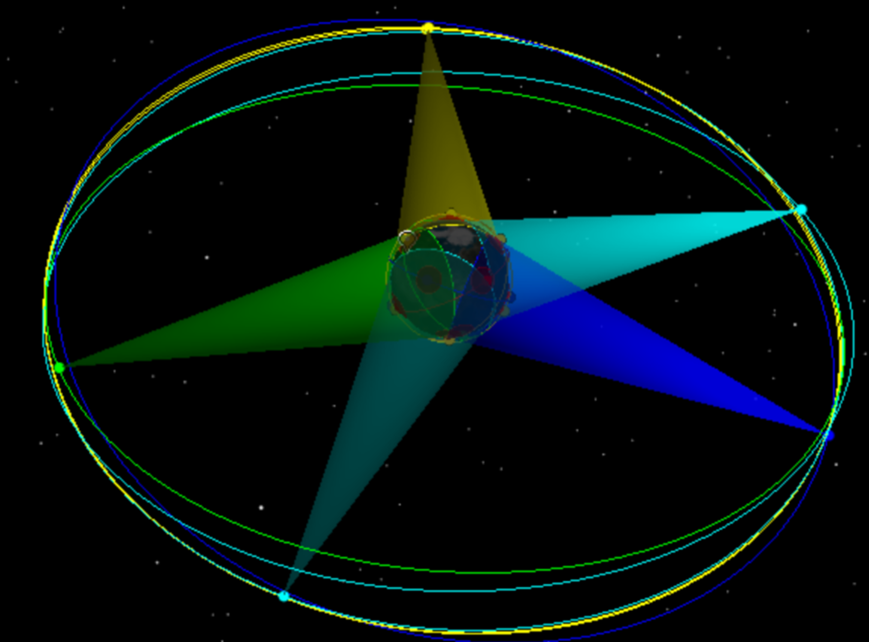
\includegraphics[width=0.5\linewidth]{images/watcher_zoom_3D_concept.png}
    \caption{\footnotesize{Watcher--Zoom two-layer constellation geometry. $\mathcal{C}_{\text{Watcher}}$ is defined as the five geostationary \emph{S-Watcher} satellites providing full-disk fire-detection coverage (FIRMS constellation, Table~\ref{tab:geo_satellites}). The $\mathcal{C}_{\text{Zoom}}$ LEO layer provides high-resolution active fire observation and is guided by the faster but coarser fire detection the geostationary Watcher layer.}}
    \label{fig:watcher_zoom_3D_concept}
\end{figure}

\begin{figure}[H]
    \centering
    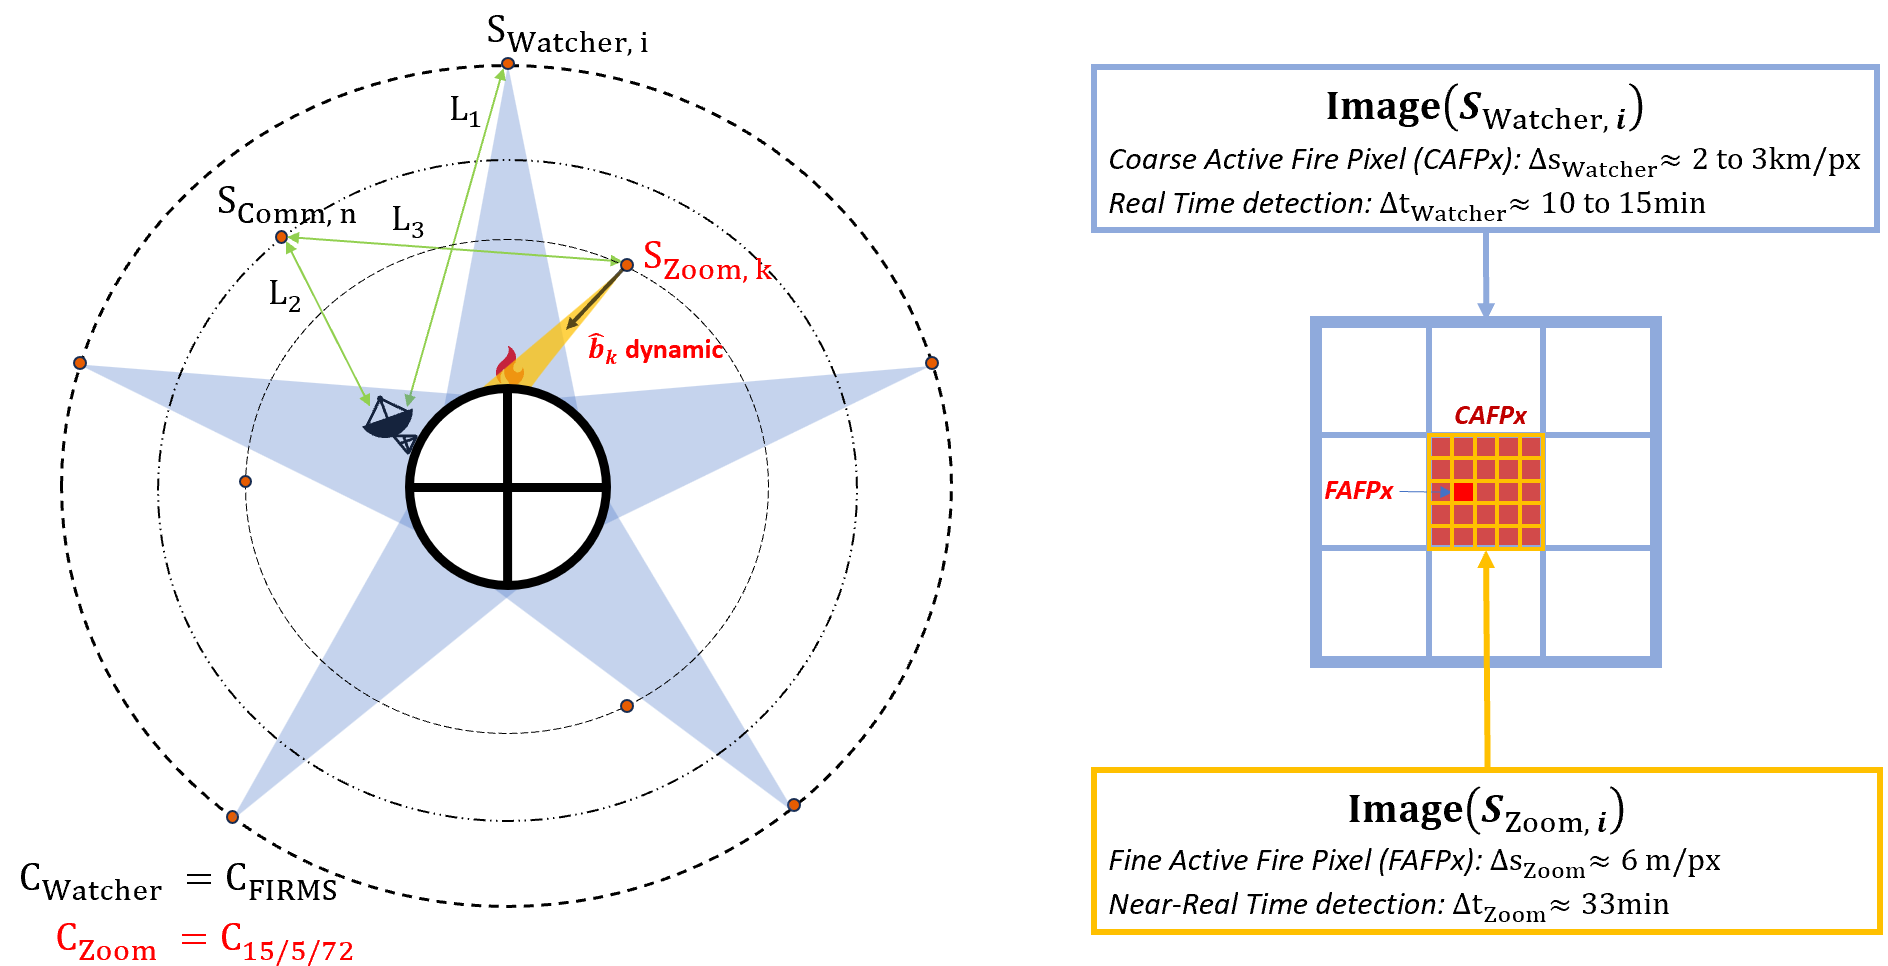
\includegraphics[width=1\linewidth]{images/proposed_watcher_zoom_concept.png}
    \caption{\footnotesize{Proposed Watcher--Zoom ``tip-and-cue'' operational concept.  \textbf{Left:} the $S_{\text{Watcher},i}$ layer detects an active fire and the alert propagates through the communication chain $\mathcal{L}_1 \to \mathcal{L}_2 \to \mathcal{L}_3$ to an $S_{\text{Zoom},k}$ satellite.  \textbf{Right:} Concept of alignment of the coarse active-fire pixel (CAFPX) from $\mathcal{I}(S_{\text{Watcher},i})$ ($\Delta s_{\text{Watcher}} \approx 1$--$3$\,km/pixel, $\Delta t_{\text{Watcher}} \approx 10$--$15$\,min) with the fine active-fire pixel (FAFPX) from $\mathcal{I}(S_{\text{Zoom},k})$ ($\Delta s_{\text{Zoom}} \approx 6$\,m/pixel, $\Delta t_{\text{Zoom}} \lesssim 30$\,min), demonstrating the tempo and spatial-resolution gain to detect active fire enabled by the fast cueing architecture.}}
    \label{fig:proposed_watcher_zoom_concept}
\end{figure}




% \begin{figure}[H]
%     \centering
%     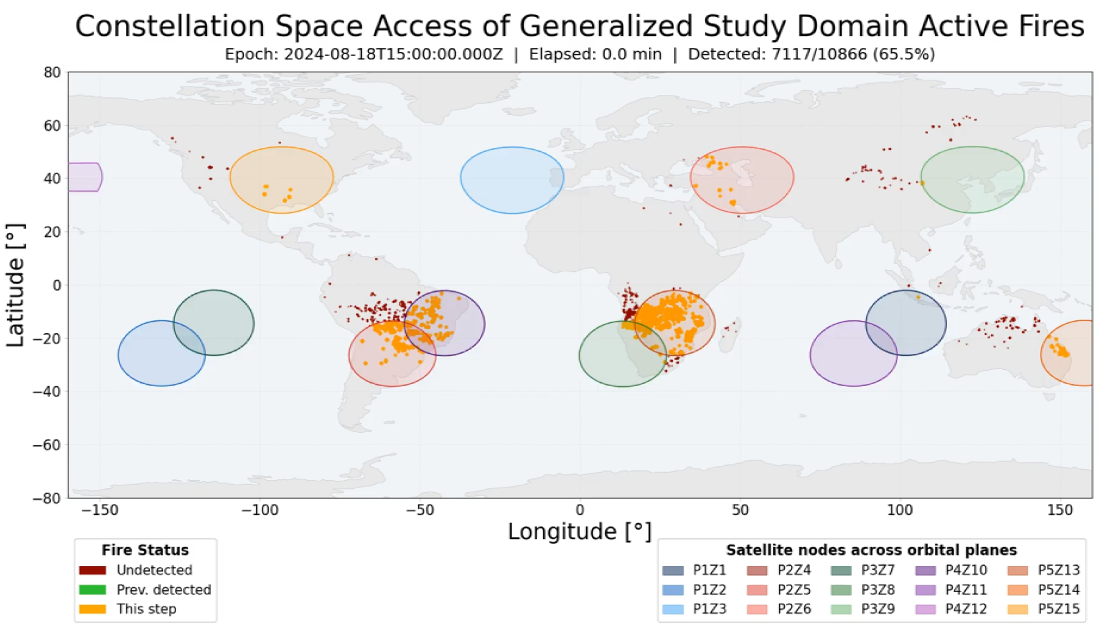
\includegraphics[width=1\linewidth]{images/concept_Watcher_Zoom_Space_access_simulation.png}
%     \caption{Enter Caption}
%     \label{fig:concept_Watcher_Zoom_Space_access_simulation}
% \end{figure}


\subsection{Constellation Architecture Initial Demonstration}
\label{sec:constellation_architecture_initial_demonstration}

With the Watcher--Zoom tip-and-cue architecture established, this subsection provides an initial demonstration of the concept through two complementary analyses: (i)~the observation-link capability of $\mathcal{C}_{\text{Zoom}}$ over real active-fire events, and (ii)~the feasibility of overlapping coarse and high-resolution fire imagery using existing satellite data as a proxy for the proposed system.

\subsubsection{Observation-Link Capability over Reference Fire Events}
\label{sec:concept_initial_observation_link_capability}

To evaluate the observation capacity of the $\mathcal{C}_{\text{Zoom}}$ layer over the $\mathcal{C}_{\text{Watcher}}$ geostationary fire-detection domain, the reference active-fire events $\Upsilon_{\text{fires}}$ defined in Section~\ref{sec:firms_dataset} are used.  These events, drawn from the FIRMS geostationary dataset, are populated over the global domain~$\mathcal{D}_{\text{global}}$, and each satellite of $\mathcal{C}_{\text{Zoom}}$ is propagated over this domain for a one-hour window.  Figure~\ref{fig:global_domain_active_fire_scan_onestep} shows the result: nearly 100\,\% of the concurrent active-fire events $\Upsilon_{\text{fires}}$ fall within the observation-link envelope at the baseline off-nadir angle $\eta_{\max} = 65^{\circ}$.

It must be noted that geometrical access does not imply a confirmed detection: actual fire observation requires a dedicated instrument with a defined swath, pointing mechanism, and collection schedule, all of which are outside the scope of this geometric study.  The simulation models the maximum effective field of view; in a higher-fidelity scenario the sensor would point within this detection envelope rather than covering it entirely.  Nonetheless, the simulator provides geometrically validated observation-link data over real fire events, establishing the foundation needed to support future instrument-level trade-offs---including sensor FOV, pointing range, swath width, image quality budgets, and onboard processing architectures such as in-orbit AI inference systems.

\begin{figure}[H]
    \centering
    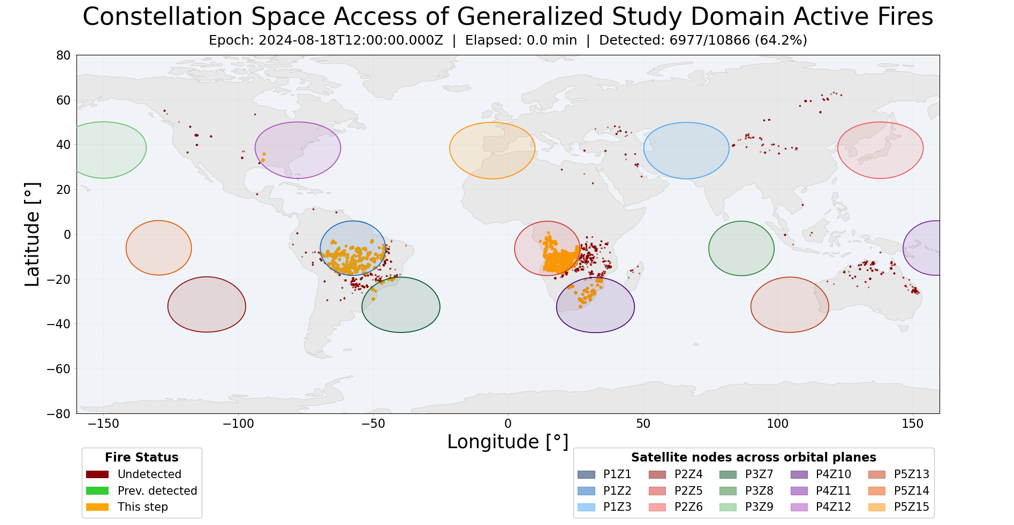
\includegraphics[width=0.75\linewidth]{images/global_domain_active_fire_scan_onestep.png}
    \caption{\footnotesize{Global-domain scan of the $\mathcal{C}_{\text{Zoom}}$ observation-link coverage over reference active-fire events~$\Upsilon_{\text{fires}}$.  Within a one-hour propagation window at $\eta_{\max} = 65^{\circ}$, nearly all concurrent global fire detections fall within the space-segment access envelope.  Geometrical access does not imply confirmed detection; the sensor footprint, pointing strategy, and collection schedule remain outside the scope of this geometric study.}}
    \label{fig:global_domain_active_fire_scan_onestep}
\end{figure}


\subsubsection{Coarse--Fine Image Overlap: Sentinel-2 as $\mathcal{C}_{\text{Zoom}}$ Proxy}
\label{sec:coarse_fine_image_overlap_demonstration}

The second demonstration evaluates the feasibility of overlapping a coarse active-fire pixel (CAFPx) from the $\mathcal{C}_{\text{Watcher}}$ layer with a high-resolution image from a LEO sensor.  Because the 15-satellite $\mathcal{C}_{\text{Zoom}}$ constellation is not yet deployed, the Sentinel-2 constellation is used as a proxy: Sentinel-2 operates at a similar LEO altitude and provides a fine active-fire pixel (FAFPx) at $\Delta s \approx 10$--$60$\,m/pixel, comparable in scale to the proposed $\mathcal{C}_{\text{Zoom}}$ GSD of $\approx 6$\,m/pixel.  The key difference is temporal resolution: Sentinel-2 revisits any given point with a five-day cadence, whereas the proposed constellation targets $\Delta t_{\text{Zoom}} \lesssim 30$\,min.

Figure~\ref{fig:proposed_watcher_zoom_initial_demonstration_w_Sentinel2_FIRMS} illustrates the concept: in the operational Watcher--Zoom architecture, $S_{\text{Watcher},i}$ provides the CAFPx that cues $S_{\text{Zoom},k}$; in this demonstration, the Sentinel-2 archive replaces $\mathcal{C}_{\text{Zoom}}$.  The algorithm proceeds as follows (Fig.~\ref{fig:fire_sanduich_Sentinel2_FIRMS_GOES_active_fire_algorithm}).  On a longitude--latitude--time domain, two Sentinel-2 archive images $\mathcal{I}(S_{\text{S2}}, t_1)$ and $\mathcal{I}(S_{\text{S2}}, t_2)$ are placed on the time axis, separated by the five-day revisit interval.  Simultaneously, the FIRMS $\mathcal{C}_{\text{Watcher}}$ constellation generates CAFPx detections every $\Delta t_{\text{Watcher}} \approx 10$--$15$\,min.  The matching criterion asks: \emph{does a Sentinel-2 image acquisition fall within $\pm\,15$\,min of a FIRMS CAFPx detection at the same location?} When this temporal coincidence is satisfied, the Sentinel-2 image has a high likelihood of containing active-fire pixels FAFPx that overlap the coarse FIRMS detection CAFPx, thereby demonstrating the tip-and-cue image-overlap concept.

\begin{figure}[H]
    \centering
    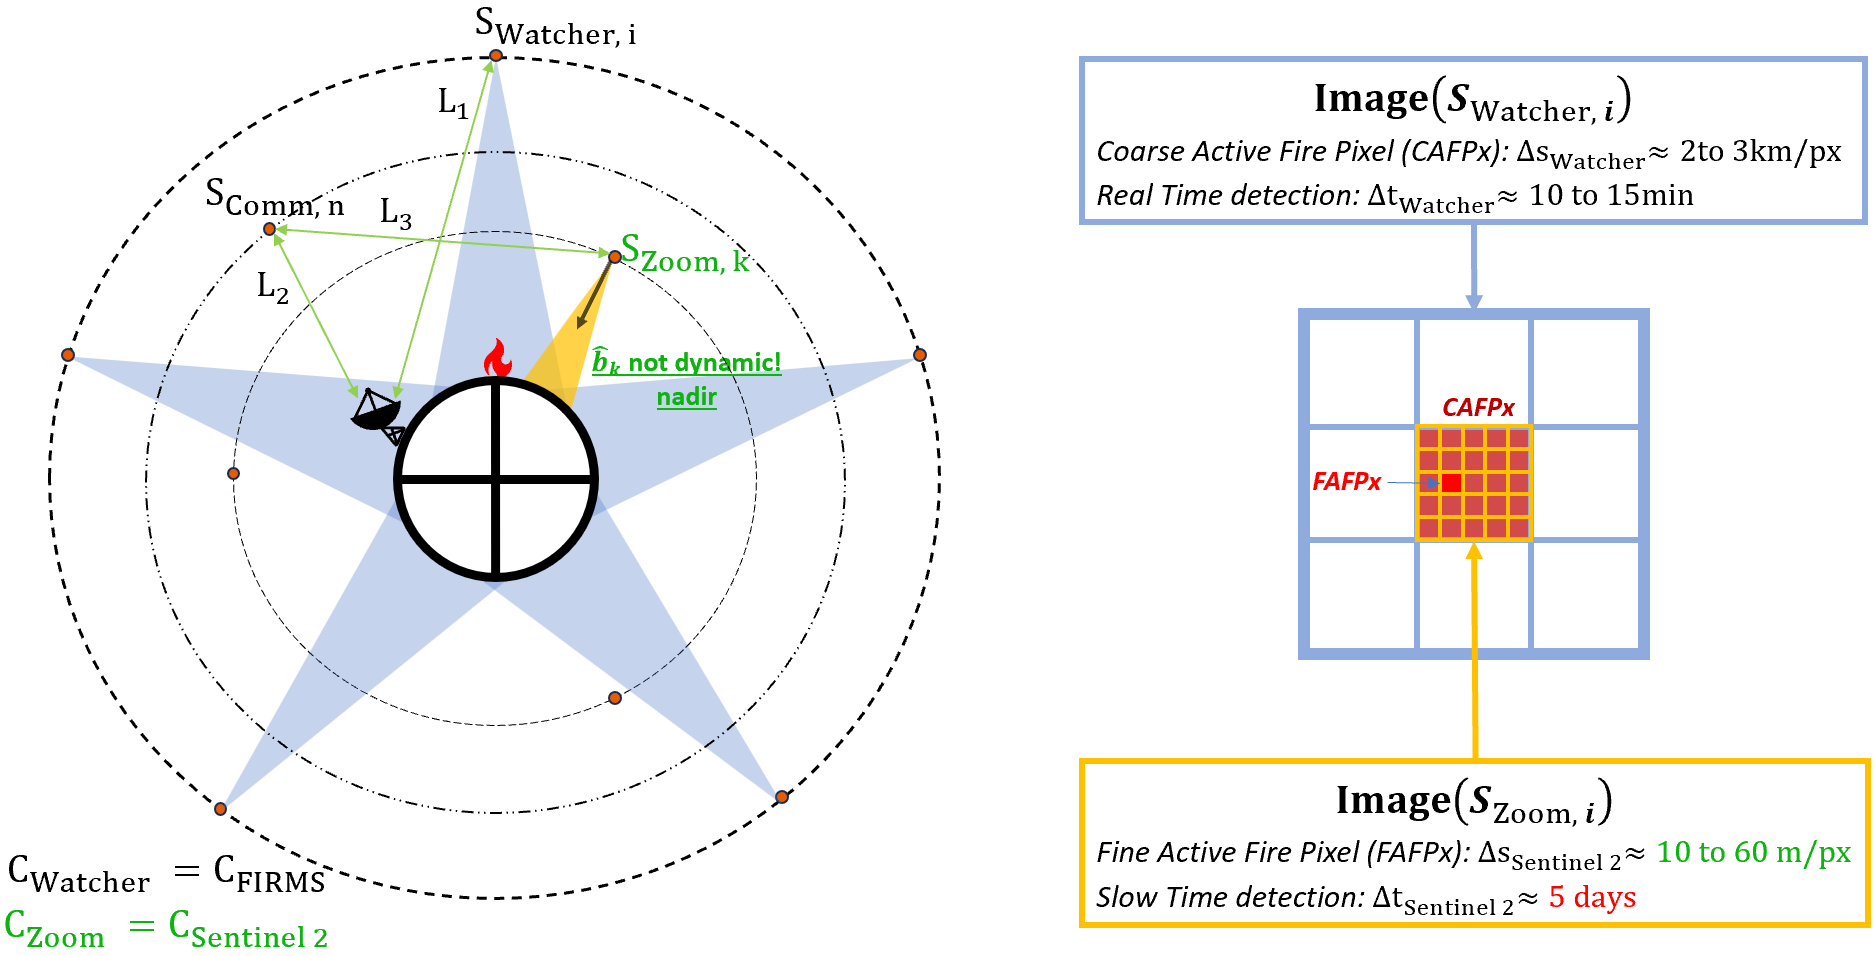
\includegraphics[width=1\linewidth]{images/proposed_watcher_zoom_initial_demonstration_w_Sentinel2_FIRMS.png}
    \caption{\footnotesize{Initial demonstration concept of the Watcher--Zoom image overlap using Sentinel-2 as a proxy for~$\mathcal{C}_{\text{Zoom}}$.  The $S_{\text{Watcher},i}$ layer (FIRMS geostationary constellation) provides the CAFPx detection ($\Delta s_{\text{Watcher}} \approx 2$--$3$\,km/pixel, $\Delta t_{\text{Watcher}} \approx 10$--$15$\,min), while the Sentinel-2 archive supplies the high-resolution counterpart (FAFPx, $\Delta s \approx 10$--$60$\,m/pixel) at a five-day revisit cadence.}}
    \label{fig:proposed_watcher_zoom_initial_demonstration_w_Sentinel2_FIRMS}
\end{figure}

\begin{figure}[H]
    \centering
    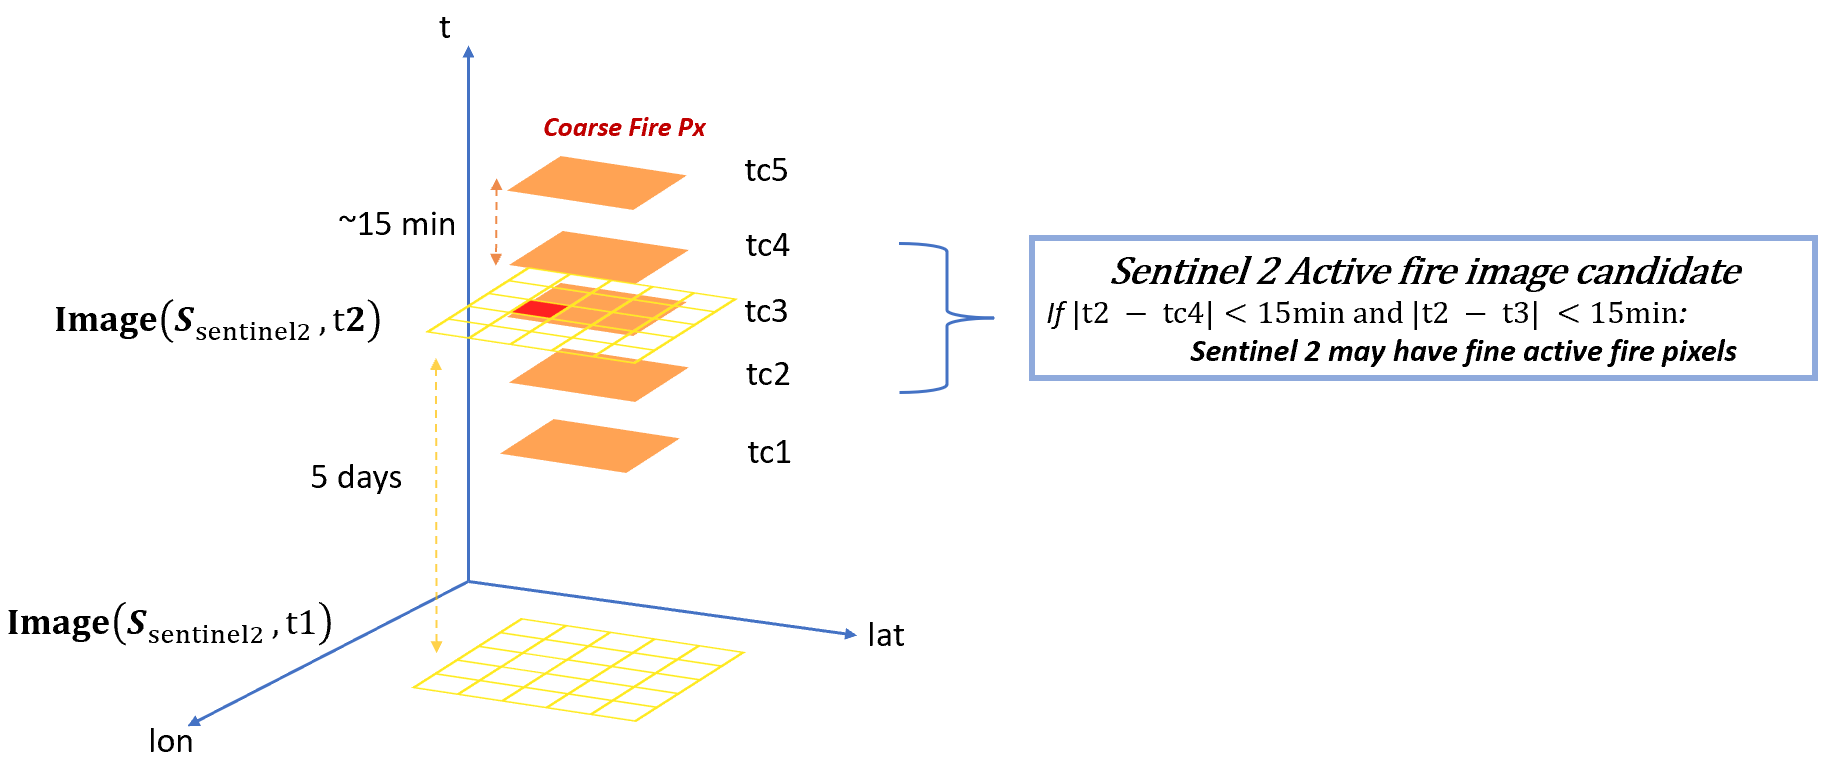
\includegraphics[width=0.8\linewidth]{images/fire_sanduich_Sentinel2_FIRMS_GOES_active_fire_algorithm.png}
    \caption{\footnotesize{Temporal-coincidence algorithm for the coarse--fine image overlap demonstration.  The longitude--latitude--time diagram shows Sentinel-2 archive images $\mathcal{I}(S_{\text{S2}}, t_1)$ and $\mathcal{I}(S_{\text{S2}}, t_2)$ on the time axis, together with the FIRMS $\mathcal{C}_{\text{Watcher}}$ CAFPx detections at $\Delta t_{\text{Watcher}} \approx 10$--$15$\,min cadence.  A match is declared when a Sentinel-2 acquisition falls within $\pm\,15$\,min of a FIRMS detection at the same location, indicating a high likelihood of active-fire pixels in the Sentinel-2 image.}}
    \label{fig:fire_sanduich_Sentinel2_FIRMS_GOES_active_fire_algorithm}
\end{figure}


Applying this temporal-coincidence scan over the full year 2024 using the Google Earth Engine Sentinel-2 archive, a total of 3062 active-fire images were identified globally (Fig.~\ref{fig:active_fire_dataset_global_2024_FIRMS_Sentinel2}).  This relatively small yield reflects the stringent five-day revisit of Sentinel-2: the probability of a temporal coincidence between a Sentinel-2 pass and a FIRMS detection within a 15-minute window is inherently low.  This scarcity underscores the need for a dedicated LEO constellation with sub-30-minute revisit to ensure systematic coarse--fine overlap.

\begin{figure}[H]
    \centering
    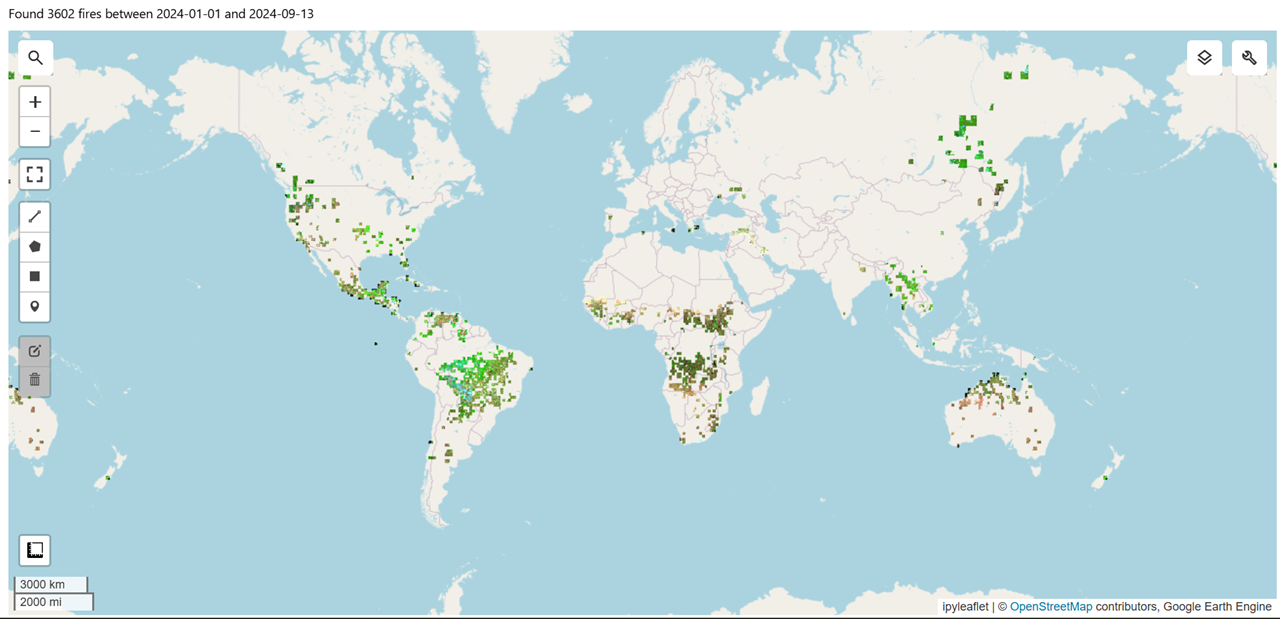
\includegraphics[width=0.8\linewidth]{images/active_fire_dataset_global_2024_FIRMS_Sentinel2.png}
    \caption{\footnotesize{Global map of the 3062 active-fire images identified in 2024 by the temporal-coincidence algorithm applied to the Sentinel-2 archive and FIRMS $\mathcal{C}_{\text{Watcher}}$ CAFPx dataset.  Each marker represents a Sentinel-2 acquisition that fell within $\pm\,15$\,min of a FIRMS geostationary fire detection, confirming coarse--fine image overlap at that location.}}
    \label{fig:active_fire_dataset_global_2024_FIRMS_Sentinel2}
\end{figure}

Two representative cases illustrate the overlap fidelity.  Figure~\ref{fig:portugal_Viseu_2024-08-16_fire_Watcher_Firms_Zoom_S2_fire_pixels} shows the only fire event captured over Portugal in 2024 by this method: a wildfire near Viseu (2024-08-16), close to the core-domain latitude $\phi \approx 40^{\circ}$\,N.  The Sentinel-2 image reveals a active fire event tt high resolution pixel level FAFPx, while the large blue pixels are the Fire Radiative Power gradient emmite by the fire($\sim\!2$\,km scale) represent the FIRMS CAFPx detections from $\mathcal{C}_{\text{Watcher}}$. Check equation \ref{eq:frp_operational} for more about FRP.  The two datasets are nearly co-located, confirming that the coarse Watcher-layer detection correctly flags the region where the high-resolution sensor observes active fire. Simulating the behaviour the tip-and-cue architecture is designed to exploit.

Figure~\ref{fig:australia_fire_2024-04-17_big} presents a second, larger-scale example: an Australian wildfire (2024-04-17) with a nearly continuous fire front extending $\sim\!37$\,km.  Fire radiative power in this event reaches $\sim\!1{,}000$\,MW, compared with $\sim\!297$\,MW for the Portuguese case, illustrating the dynamic range of fire intensity the system must accommodate.

Together, these two demonstrations confirm that: (i)~the $\mathcal{C}_{\text{Zoom}}$ observation-link geometry covers nearly all global active-fire events within a one-hour window, and (ii)~real satellite data validate that a coarse geostationary detection can reliably flag the location where a high-resolution LEO sensor observes active fire.  What the current demonstrations lack is the dynamic pointing capability .  Realising the operational architecture therefore requires the communication layer~$\mathcal{C}_{\text{Comm}}$ to relay cueing commands from the Watcher layer to the Zoom layer in near-real time, a component addressed in subsequent system-level design.

\begin{figure}[H]
    \centering
    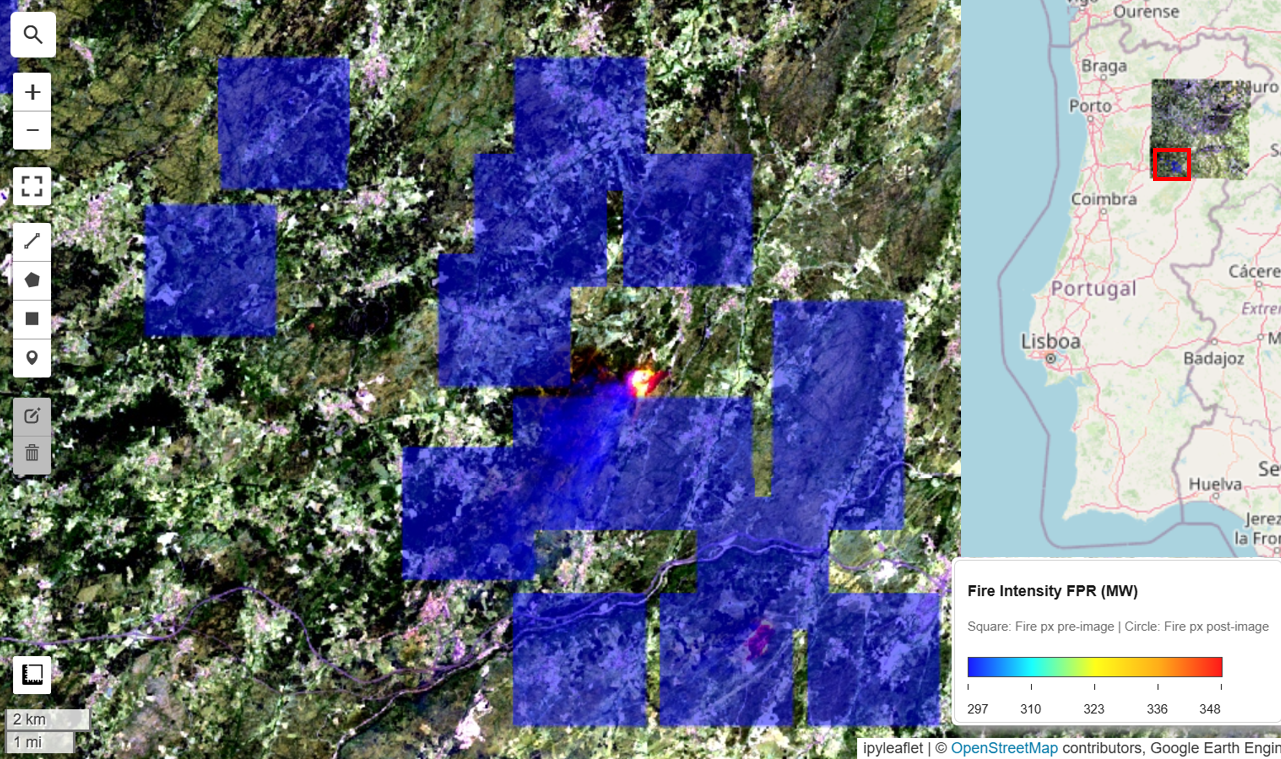
\includegraphics[width=0.9\linewidth]{images/portugal_Viseu_2024-08-16_fire_Watcher_Firms_Zoom_S2_fire_pixels.png}
    \caption{\footnotesize{Coarse--fine image overlap for the Viseu (Portugal) wildfire, 2024-08-16.  The Sentinel-2 per-pixel fire-intensity gradient (FAFPx, $\Delta s \approx 10$--$60$\,m/pixel) is overlaid with the FIRMS $\mathcal{C}_{\text{Watcher}}$ coarse active-fire pixels (CAFPx, $\Delta s \approx 2$\,km/pixel, blue).  The near co-location of the two datasets demonstrates the feasibility of the Watcher-layer cueing concept: the CAFPx correctly flags the region where high-resolution active fire is observed.  Fire radiative power $\approx 297$\,MW.}}
    \label{fig:portugal_Viseu_2024-08-16_fire_Watcher_Firms_Zoom_S2_fire_pixels}
\end{figure}

\begin{figure}[H]
    \centering
    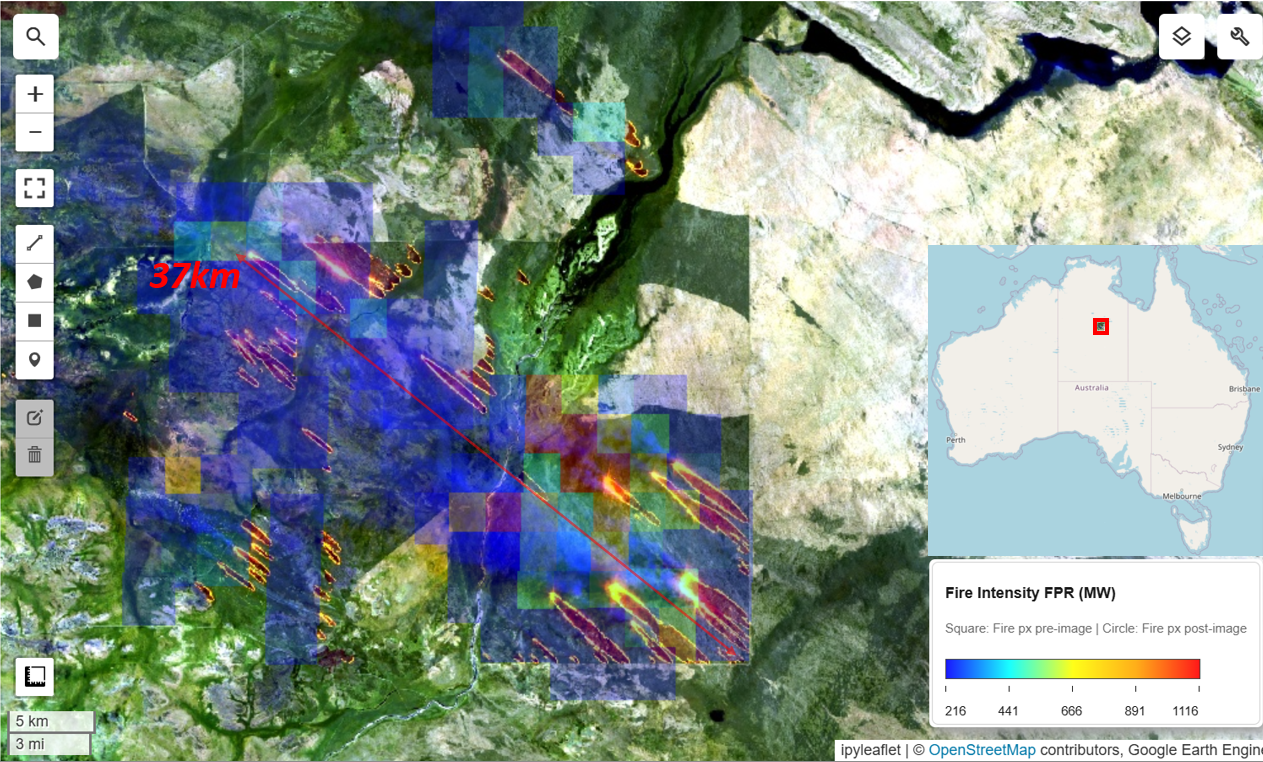
\includegraphics[width=0.9\linewidth]{images/australia_fire_2024-04-17_big.png}
    \caption{\footnotesize{Coarse--fine image overlap for an Australian wildfire, 2024-04-17.  The fire front extends $\sim\!37$\,km with fire radiative power reaching $\sim\!1{,}000$\,MW.  As in the Portuguese case, the FIRMS CAFPx detections (blue, $\Delta s \approx 2$\,km/pixel) align with the Sentinel-2 FAFPx active-fire pixels, confirming the tip-and-cue overlap concept at a substantially larger fire scale.}}
    \label{fig:australia_fire_2024-04-17_big}
\end{figure}



% \section{Conceptual Payload \& Communications
% Requirements}\label{92-conceptual-payload--communications-requirements}
% \fxwarning{Write brief section on payload and communication limitations: top-level imaging payload requirements and communication constraints between Zoom layer and ground/AGIF system. Keep concise---detailed sizing is future work.}

% \section{Concept of Operations
% (CONOPS)}\label{93-concept-of-operations-conops}
% \fxwarning{Write CONOPS narrative: day-in-the-life scenario from fire detection in Portugal to data delivery to AGIF fire-combat system. Add architecture diagram connecting Watcher layer $\to$ Zoom layer $\to$ ground segment $\to$ AGIF.}


% % --- Chapter 10: Discussion ---
\chapter{Discussion}\label{chapter-10-discussion}

This chapter interprets the results presented in and Chapters~\ref{73-constellation-architectures-design} and Chapters~\ref{chapter-9-the-proposed-system-concept}, connects them to the research questions posed in Chapters~\ref{chap:partI_intro_back}. The discussion is organised into three sections: analysis of the proposed solution and its contributions, system feasibility and open challenges, and limitations of the present study.

%------------------------------------------------------------------
\section{Analysis of the Proposed Solution}\label{sec:discussion-analysis}
%------------------------------------------------------------------

The central research question of this thesis asked: \emph{what satellite constellation design can close the spatiotemporal gap achieving roughly 30-minute revisit and approximately 6~m ground resolution over continental Portugal providing orbital fire observation, improving fire-weather and fire-spread prediction for Portugal?} A secondary question is: \emph{What coverage reach the proposed constellation provide over global fire-prone regions?} Three contributions answer this question.

\subsection{Contribution~1: RGTO-Based Fire Detection Constellation Tuned for Portugal}

The first contribution is the design of $\mathcal{C}_{\text{Zoom}} = \mathcal{C}_{15/5/72}$: a 15-satellite Walker Repeating Ground-Track Orbit (RGTO) constellation whose inclination ($i = 40.20^{\circ}$) matches the latitude of continental Portugal, creating a resonant daily revisit pattern. The constellation geometry is shown in Fig.~\ref{fig:GaiaFireeyes_Constellation3}, with the orbital seed elements defined in Eq.~\ref{eq:RGTO_2_coimbra} and their resulting maps, revisit patterns, and observation links in Figs.~\ref{fig:RGTO_maps_Coimbra_One_day}, \ref{fig:RGTO_metrics_Coimbra_One_day}, \ref{fig:RGTO_metrics_Coimbra_Seven_days}, \ref{fig:temporal_res_P1S1}, \ref{fig:obs_links_5planes}; the Walker architecture is detailed in Tables~\ref{tab:walker_c15}, \ref{tab:Czoom_eta_configurations}, and~\ref{tab:rgto_family_coimbra}. Following the results metrics over Portugal's core domain~$\mathcal{D}_{\mathrm{core}}$ described in section \ref{sec:portugal_core_domain_metrics_derive_from_global_domain_results}, the constellation delivers $\approx 6$\,h\,day$^{-1}$ of temporal coverage, an average revisit of $\approx 21$\,min (worst-case $\approx 35$\,min, best-case $\approx 12$\,min), and GSD~$< 6$\,m\,px$^{-1}$---satisfying mission requirements R7 and R8. The resonance mode $\tau = 15/1$ at $h \approx 488$\,km yields four daily passes per satellite: two near nadir (elevation ${>}\,75^{\circ}$, best image resolution) and two at lower elevations (${>}\,30^{\circ}$). Benchmarked against the typical SpaceX Transporter rideshare SSO (Appendix~\ref{app:sso_orbit}), the RGTO delivers $\approx 1.75\times$ the daily coverage rate  (Figs.~\ref{fig:rgtoVSsso_7day_prop_maps}--\ref{fig:rgtoVSsso_7day_prop_old}). An SSO-based constellation would therefore require roughly twice as many satellites to achieve equivalent temporal coverage of the proposed RGTO-based architecture. To our knowledge, this is the first RGTO constellation specifically designed for Portuguese monitoring.

\subsubsection{RGTO Resonance Family and Multi-Layer Potential}

Beyond the selected $\tau = 15/1$ mode, the resonance analysis produced as contribution a family of RGTO modes for Portugal (Table~\ref{tab:rgto_family_coimbra}), spanning low earth orbit bands ($\sim\!488$\,km) to MEO ($\sim\!1623$\,km), but it grows farther than this modes. This family is generalized to the full inclination range $i \in [0^{\circ},\,90^{\circ}]$ in Fig.~\ref{fig:RGTO_1day_resonance}, making the resonance curves applicable to any target latitude worldwide. The existence of multiple co-resonant altitudes above the same target enables multi-layer architectures in which satellites at different altitudes share the same ground-track repeat period, producing synchronised passes over a common region---for example, pairing a high-resolution imaging layer with a broader-swath monitoring or data-relay layer, both revisiting Portugal on a coordinated daily schedule.

\subsection{Contribution~2: Watcher-Zoom Two-Layer Architecture}

The second contribution is the \emph{Watcher-Zoom} (tip-and-cue) architecture proposed in section~\ref{sec:proposed_architecture}. No prior constellation design, to our knowledge, combines existing geostationary fire-watch assets (GOES, Meteosat, Himawari---the ``Watcher'' layer, $\mathcal{C}_{\text{Watcher}}$) with a dedicated agile LEO constellation (the ``Zoom'' layer, $\mathcal{C}_{\text{Zoom}}$) for high-resolution follow-up imaging of detected fire events.

This architecture exploits an important asymmetry: the GEO layer already provides near-global, continuous monitoring with temporal resolution trending toward sub 10 minutes cadence, but at coarse spatial resolution ($\sim$0.5--3~km), as shown insection \ref{sec:geolayer_new_gen}. Rather than duplicating wide-area surveillance in LEO, the Zoom layer receives tip-off cues from the Watcher layer and performs rapid, narrow-field-of-view pointing toward confirmed hotspot locations. This separation of roles reduces the optical and data requirements on the LEO segment. In principle, each Zoom satellite needs only to transmit fire-event data (detected/not-detected, geolocation, and a small image patch) rather than full-swath imagery, enabling lightweight communication links and a spacecraft with less energy and computational demands.

The Zoom layer concept aligns with the current trend toward CubeSat-class agile imagers: small, rapidly slewing platforms equipped with narrow-FOV sensors and compact optical or radio terminals. As the GEO watcher instruments continue to improve in temporal and spatial resolution, the tip latency of the architecture decreases without any redesign of the LEO segment.

\subsubsection{Initial Watcher-Zoom Demonstration and Data Backbone for Future Engineering Models}

Using FIRMS as a proxy for $\mathcal{C}_{\text{Watcher}}$ and Sentinel-2 for $\mathcal{C}_{\text{Zoom}}$, a temporal-coincidence scan of the full year 2024 (Section~\ref{sec:coarse_fine_image_overlap_demonstration}) identified 3062~coarse-fine overlap events globally (Fig.~\ref{fig:active_fire_dataset_global_2024_FIRMS_Sentinel2}), including a wildfire near Viseu, Portugal (Fig.~\ref{fig:portugal_Viseu_2024-08-16_fire_Watcher_Firms_Zoom_S2_fire_pixels}) and a $\sim\!37$\,km fire front in Australia (Fig.~\ref{fig:australia_fire_2024-04-17_big}), confirming that a coarse Watcher alert reliably flags the region where a high-resolution LEO sensor observes active fire.  That only one Portuguese fire event appears among 3062~global matches from a full year underscores the limitation of Sentinel-2's five-day revisit; a dedicated sub-30-minute constellation would increase the yield of actionable high-resolution fire observations by orders of magnitude.  The demonstration infrastructure---FIRMS fire timelines, Sentinel-2 spectral/spatial fire scenes, and the $\mathcal{C}_{\text{Zoom}}$ orbital simulation (Chapter~\ref{73-constellation-architectures-design})---together form the data backbone from which future engineering models can be derived, enabling sensor requirements, pointing-agility constraints, and field-of-view budgets to be traded against real observational data rather than synthetic assumptions.

%%% ----------------------------------------------------------------
%%% Contribution 3
%%% ----------------------------------------------------------------
\subsection{Contribution~3: Constellation Coverage of Global Fire-Prone Regions}

The third contribution is a constellation that cover global fire prone regions described in section \ref{sec:zoom_layer} and discussed here. The parametric analysis of the $\mathcal{C}_{\text{Zoom}}$ constellation against the sensor off-nadir angle~$\eta$ (Section~\ref{sec:zoom_layer}, Table~\ref{tab:zoom_layer_configurations}) shows that the minimum spacecraft count ($T = 15$) for a 30-min revisit over Portugal requires $\eta \approx 65^{\circ}$; restricting $\eta$ to $30^{\circ}$ nearly doubles the constellation ($T = 27$), and $\eta = 15^{\circ}$ triples it ($T = 42$).  From this single design choice---optimising for $\mathcal{D}_{\mathrm{core}}$ at the minimum viable size---the coverage footprint extends naturally to the global fire-prone domain~$\mathcal{D}_{\mathrm{global}}$.

A detailed analysis of the coverage metrics over $\mathcal{D}_{\mathrm{global}}$ quantifies this extension.  The temporal-coverage maps (Fig.~\ref{fig:c_zoom_global_Tcovera_eta63}), filtered through recurrent and occasional fire-prone region masks (Fig.~\ref{fig:c_zoom_global_Tcoverage_FRP_groups_Spatial_Mask}), yield the global fire-prone coverage map (Fig.~\ref{fig:c_zoom_global_FRP_recurrent_ocasional_Tcoverage_eta63}).  The temperate belt ($\phi \approx \pm\,30^{\circ}$--$45^{\circ}$)---southern Europe, the western United States, south-eastern Australia, southern South America, and southern Africa---receives $T_{\text{cov}} \approx 6$--$7$\,h\,day$^{-1}$; the equatorial belt---Amazonia, sub-Saharan Africa, and maritime South-East Asia---retains $T_{\text{cov}} \geq 3.5$\,h\,day$^{-1}$ (country-level enumeration in Section~\ref{sec:fpr_coverage_analysis}).  The constellation also sustains a high revisit cadence globally: across $\phi \approx \pm\,20^{\circ}$--$40^{\circ}$, the worst-case gap stays $\Delta t_{\max} \approx 30$\,min, with the best average revisit $\Delta t_{\text{avg}} \approx 21$\,min at Portugal $\phi \approx 40^{\circ}$\,N (Section~\ref{sec:portugal_core_domain_metrics_derive_from_global_domain_results}, Fig.~\ref{fig:c_zoom_metrics_latitude_profile_not_norm}).  At the equatorial fringe ($\phi \approx \pm\,15^{\circ}$), the gap widens to $\Delta t_{\max} \approx 115$\,min and $\Delta t_{\text{avg}} \approx 40 - 50$\,min (Fig.~\ref{fig:c_zoom_avg_revisit}), yet both values remain well below the revisit of current polar-orbiting fire-detection systems at comparable spatial resolution.

This archicteture misses boreal fire active regions, but it can be complementary to high-latitude programmes---such as Canadian and Australian systems---that address biomes outside the RGTO inclination band, opening the prospect of an internationally coordinated fire-observation network.  The central conclusion of this contribution is that a constellation originally sized for Portuguese wildfire monitoring simultaneously services the majority of fire-prone nations worldwide, transforming a regional mission into a global one.

%%% ----------------------------------------------------------------
%%% Comparison with the State of the Art
%%% ----------------------------------------------------------------
\subsection{Comparison with the State of the Art}

The gap analysis of Figure~\ref{fig:gap_satellite_constellations_spatial_temporal_plot} established that no operational or planned mission simultaneously provides sub-hour revisit and metre-class thermal resolution over any regional domain.  The proposed system closes this gap by combining three mutually reinforcing elements: an RGTO orbit that concentrates coverage on temperate fire-prone regions---primarily Portugal---with an average revisit of $\approx 21$\,min and roughly half the satellite count of an equivalent SSO design; a Watcher-Zoom architecture that leverages existing GEO fire-watch assets to dynamically aim to fire spots instead of duplicating wide-area surveillance in LEO; and their joint result---a natural extension to global fire-prone regions delivering $T_{\text{cov}} \approx 6$--$7$\,h\,day$^{-1}$ over the temperate belt and ${\geq}\,3.5$\,h\,day$^{-1}$ over equatorial fire zones, with sub-hour revisit cadence ($\sim\!30$\,min on average) across most covered latitudes.  No system in the current or planned inventory offers this combination from a single 15-satellite constellation, making the proposed architecture a step change relative to the state of the art.

%------------------------------------------------------------------
\section{System Feasibility and Challenges}\label{sec:discussion-feasibility}
%------------------------------------------------------------------

\subsection{Feasibility Factors}

Several trends in the space industry support the practical viability of the proposed system:

\begin{itemize}
    \item \textbf{Launch access.} The baseline altitude of $\approx$488~km is well within the envelope of current rideshare services on reusable launchers, which have driven per-kilogram costs to historic lows. The RGTO, moderate-inclination orbit is also compatible with dedicated small-launcher providers.
    \item \textbf{Platform maturity.} CubeSat and small-satellite buses with three-axis stabilisation, agile slew capability, and COTS thermal/optical sensors are emerging, reducing non-recurring engineering costs. Also reaching the $GSD~6m/px$ is possible in small sats .
    \item \textbf{Existing infrastructure.} The Watcher layer relies entirely on operational GEO assets; no new geostationary satellites need to be launched. Active-fire products from GOES, Meteosat, and Himawari are freely available with latencies already in the minute-to-sub-minute range.
    \item \textbf{Debris environment.} At 488~km, residual atmospheric drag ensures natural de-orbit within a few years even without active disposal, consistent with current space-debris mitigation guidelines and the emerging regulatory trend toward shorter orbital lifetimes.
\end{itemize}

\subsection{Open Challenges}

Three principal challenges remain:

\begin{enumerate}
    \item \textbf{Inter-layer communication.} Connecting the Zoom layer to ground users  requires a data relay path. Options include direct ground-station contact during passes, or relay through a commercial LEO broadband constellation. Neither option was sized in this work; a link-budget analysis and latency assessment are necessary.
    \item \textbf{Agile pointing mechanism.} The tip-and-cue concept demands rapid slew-and-settle performance of each Zoom satellite. Achieving sub-degree pointing accuracy within seconds on a CubeSat-class platform is feasible with current reaction-wheel and star-tracker technology, but detailed design and jitter analysis are required.
    \item \textbf{Station-keeping.} The RGTO resonance condition drifts after approximately 30~days without orbit-maintenance manoeuvres (Chapter~\ref{app:station_keeping}). Maintaining the ground-track repeat pattern requires $\sim$4~burns per year, implying a propulsion subsystem whose mass and power budget were not traded in this study. Detailed study is need to further explore the impacts of orbital stability and station-keeping on the constellation design and operational concept.
    \item  \textbf{Thermal Sensor in Small Spacecraft.} As the Fire Radiant Power is measure in the Middle Infrared (MIR) spectral range, the thermal sensor must be designed to operate in this range as required in Equation \ref{eq:frp_operational}. The design must consider factors such as thermal management, calibration, and sensitivity to ensure accurate fire detection and characterization which can be challenge in small volume satellites. 
\end{enumerate}

%------------------------------------------------------------------
\section{Limitations of the Study}\label{sec:discussion-limitations}
%------------------------------------------------------------------

The scope of this work was deliberately bounded at the Pre-Phase~A / Phase~A level of the systems-engineering lifecycle. The following limitations should be considered when interpreting the results; they also define the starting points for future work (Chapter~\ref{chapter-11-conclusion-and-future-work}).

\paragraph{Cluster~A: Sensor and Imaging Fidelity.}
The analysis evaluated geometric observational access (the visibility cone between satellite and target) but did not simulate the imaging chain. No modulation-transfer-function (MTF), signal-to-noise-ratio (SNR), or motion-blur analysis was performed. The image quality at large off-nadir angles remains uncharacterised. Spectral-band selection and radiometric sensitivity were likewise not traded.

\paragraph{Cluster~B: Operations and Communications.}
No communications link budget, energy budget, or operational task-scheduling model was developed. The simulations quantify \emph{when} and \emph{where} an observation link is geometrically possible, but do not derive the full set of system requirements for an operational mission (e.g., data volume, onboard storage, duty cycling, or ground-segment capacity).

\paragraph{Cluster~C: Orbital Maintenance, Manouvers and Propagation.}
Station-keeping was analysed at the level of altitude-decay rate and burn frequency, but the propulsion subsystem was not sized. No conjunction-screening or collision-avoidance analysis was performed. The atmospheric-drag model used a simplified exponential atmosphere rather than a time-varying density model. The manoverus capability for the dynamical sensor required for the Watcher-Zoom architecture was not explored.

\medskip

\noindent Despite these limitations, the simulation framework---combining GMAT high-fidelity propagation ($c_{8,8}$ geopotential plus drag), satellite-derived fire-pixel datasets, and the observational-link geometry model---provides a reusable platform from which the above requirements can be iteratively derived in subsequent design phases.




% % --- Chapter 11: Conclusion and Future Work ---
\chapter{Conclusion and Future Work}
\label{chapter-11-conclusion-and-future-work}

This chapter closes the thesis in three parts: a summary of the research methodology and the path from problem statement to the three contributions; a conclusion that directly answers the two research questions and positions the proposed architecture against the state of the art; and recommendations for future work organized into payload, communications, and mission-simulation themes.

%------------------------------------------------------------------
\section{Summary of Research}\label{sec:conclusion-summary}
%------------------------------------------------------------------

Wildfire risk in Mediterranean Europe --- particularly in Portugal --- has intensified, with longer fire seasons, larger burned areas, and extreme events that overwhelm tactical decision windows. Current satellite services face a resolution--revisit--latency gap: geostationary platforms monitor continuously but at coarse resolution, while polar LEO missions offer finer imagery at revisit intervals of hours to days. This thesis asked: \emph{What fire observation satellite constellation design can close the spatiotemporal gap, achieving roughly 30-minute revisit and approximately 6~m ground resolution over continental Portugal?} A secondary question is: \emph{What coverage does the proposed constellation provide over global fire-prone regions?}

The study began with a characterisation of the resolution--revisit--latency gap in current satellite fire-detection (Chapter~\ref{c1_introduction}), followed by the definition of mission requirements and the identification of global fire-prone domains from satellite-derived active-fire records (Chapter~\ref{chapter-2-the-wildfire-challenge-and-study-case-definition-from-global-threat-to-local-data-needs}).  A Repeating Ground-Track Orbit resonance analysis, generalised to arbitrary target latitudes, produced a family of RGTO modes for continental Portugal; the selected mode was embedded in a Walker constellation framework, and a parametric study of the sensor off-nadir angle determined the minimum spacecraft count for the required revisit cadence (Chapter~\ref{73-constellation-architectures-design}).  High-fidelity GMAT propagation validated orbital stability, and an observational-link geometry model quantified temporal coverage, revisit statistics, and ground sampling distance over both the Portuguese core domain and a global fire-prone domain (Chapter~\ref{chapter-9-the-proposed-system-concept}).  In parallel, a temporal-coincidence analysis of geostationary and multispectral LEO fire imagery demonstrated the coarse-to-fine tip-and-cue detection chain empirically (Chapter~\ref{sec:proposed_architecture}).  These elements converged into three contributions: an RGTO constellation tuned for Portugal, a two-layer \emph{Watcher-Zoom} architecture coupling existing geostationary fire-watch assets with an agile LEO segment, and a quantitative assessment of the constellation's natural extension to global fire-prone regions.



%------------------------------------------------------------------
\section{Conclusion}\label{sec:conclusion-answer}
%------------------------------------------------------------------

The constellation $\mathcal{C}_{\text{Zoom}} = \mathcal{C}_{15/5/72}$---fifteen satellites in five planes at approximately 488~km, inclination matched to Portugal---delivers an average revisit of roughly 21~minutes (worst-case about 35~minutes) and a ground sampling distance below 6~m per pixel, satisfying requirements \reqRef{R7} and \reqRef{R8}.  The orbit resonance concentrates passes over the target latitude, yielding roughly twice the daily coverage of a comparable Sun-Synchronous Orbit with half the satellite count.  The \emph{Watcher-Zoom} tip-and-cue layer complements this design: existing geostationary fire-watch platforms (GOES, Meteosat, Himawari) provide coarse alerts that cue the LEO satellites for rapid, narrow-field imaging of confirmed hotspots, so each satellite transmits only fire-event data rather than full-swath imagery.   A demonstration of the Watcher-Zoom concept was conducted by testing coarse-to-fine chain image alignment of fire detections using geostationary coarse but fast images from FIRMS and Sentinel-2's slower images with high spatial resolution, confirming the concept.

Designed for Portugal at the minimum viable size, the coverage footprint extends naturally across the globe.  The temperate belt — southern Europe, the western United States, southeastern Australia, southern Africa — receives 6 to 7 hours of daily coverage with worst-case revisit gaps of about 30 minutes.  At the equatorial fringe---Amazonia, sub-Saharan Africa, maritime South-East Asia---coverage persists above 3.5 hours per day with an average revisit around 40 to 50 minutes, still outperforming current polar-orbiting fire sensors at comparable resolution.  A constellation sized for one country, therefore, services the majority of fire-prone nations, turning a regional mission into a global one.

No known Earth-observation constellation reviewed in this study achieves a fire-detection performance combining sub-30-minute revisit with metre-scale thermal resolution over Portugal or any other fire-prone region examined herein.  By uniting a resonant orbit, a geostationary-cued tip-and-cue layer, and their emergent global reach, the proposed architecture closes this gap from just fifteen satellites---offering regions facing the same wildfire threat a platform for cooperative observation.  This work lays the scientific foundation for a next-generation \emph{Satellite Constellation for Fast Fire Detection: Mission Design for Portugal Covering Global Fire-Prone Regions}.

%------------------------------------------------------------------
\section{Recommendations for Future Work}\label{sec:conclusion-future}
%------------------------------------------------------------------

The following recommendations trace a path from component-level design to full mission validation.

\subsection{Payload and Imaging}

\begin{enumerate}
    \item \textbf{End-to-end image simulator and payload constraints.} The FIRMS active-fire dataset, Sentinel-2 fire-image archive, and orbital simulation provide the inputs for an end-to-end image simulator of the Watcher-Zoom concept, enabling quantitative derivation of spectral-band selection, radiometric sensitivity, pointing-agility requirements, and the communications budget, bridging this scientific study into the engineering domain.
    \item \textbf{Image-quality simulation.} Model the imaging chain---motion blur, jitter, and off-nadir degradation---to determine the maximum usable field of view and achievable resolution under realistic attitude-control performance.
    \item \textbf{Co-design with machine vision.} Investigate co-design of the optical payload with onboard machine-learning models; a lower raw resolution may be acceptable if a trained model can reliably detect fire signatures and smoke plumes on the sensor output, reducing hardware complexity and downlink volume.
\end{enumerate}

\subsection{Communications and Autonomy}

\begin{enumerate}
    \item \textbf{Ground-segment and relay architecture.} Design the end-to-end communications path from the Zoom layer to fire-management end users, comparing direct ground-station contact, inter-satellite optical links, and relay through commercial LEO broadband constellations.
    \item \textbf{Onboard autonomy.} Develop autonomous operations concepts---onboard fire detection, dynamic re-tasking of the pointing system, and autonomous channel acquisition---to minimise ground-in-the-loop latency.
\end{enumerate}

\subsection{Mission Simulation and Scaling}

\begin{enumerate}
    \item \textbf{Full mission scenario.} Extend the geometric-access simulation to encompass sensor scheduling, detection probability, relay-chain data propagation, and integration with ground-based fire-management systems.
    \item \textbf{Station-keeping and propulsion.} Size the propulsion subsystem required to maintain RGTO resonance over the mission lifetime, and perform conjunction-screening and collision-avoidance analysis.
    \item \textbf{Global extension and cost--benefit analysis.} Evaluate constellation performance over the full global fire-prone domain $\mathcal{D}_{\mathrm{global}}$ and develop a cost--benefit model quantifying the socio-economic impact of reduced fire-detection latency.
\end{enumerate}



%% ======================================================================
%% BACKMATTER
%% ⚑ Purpose: references and appendices (post-content).
%% ======================================================================


% --- Part IV: APPENDICES ---
% ----------------------------------------
% The 'appendices' environment (from the appendix package loaded with
% [toc,page]) automatically inserts a separator page and a ToC entry,
% and switches chapter numbering to A, B, C, …
\begin{appendices}

\chapter{Figures}
\label{appendix-figures}


% \section{Burned Area Trends and Correlations}

% \begin{figure}[H]
%     \centering
%     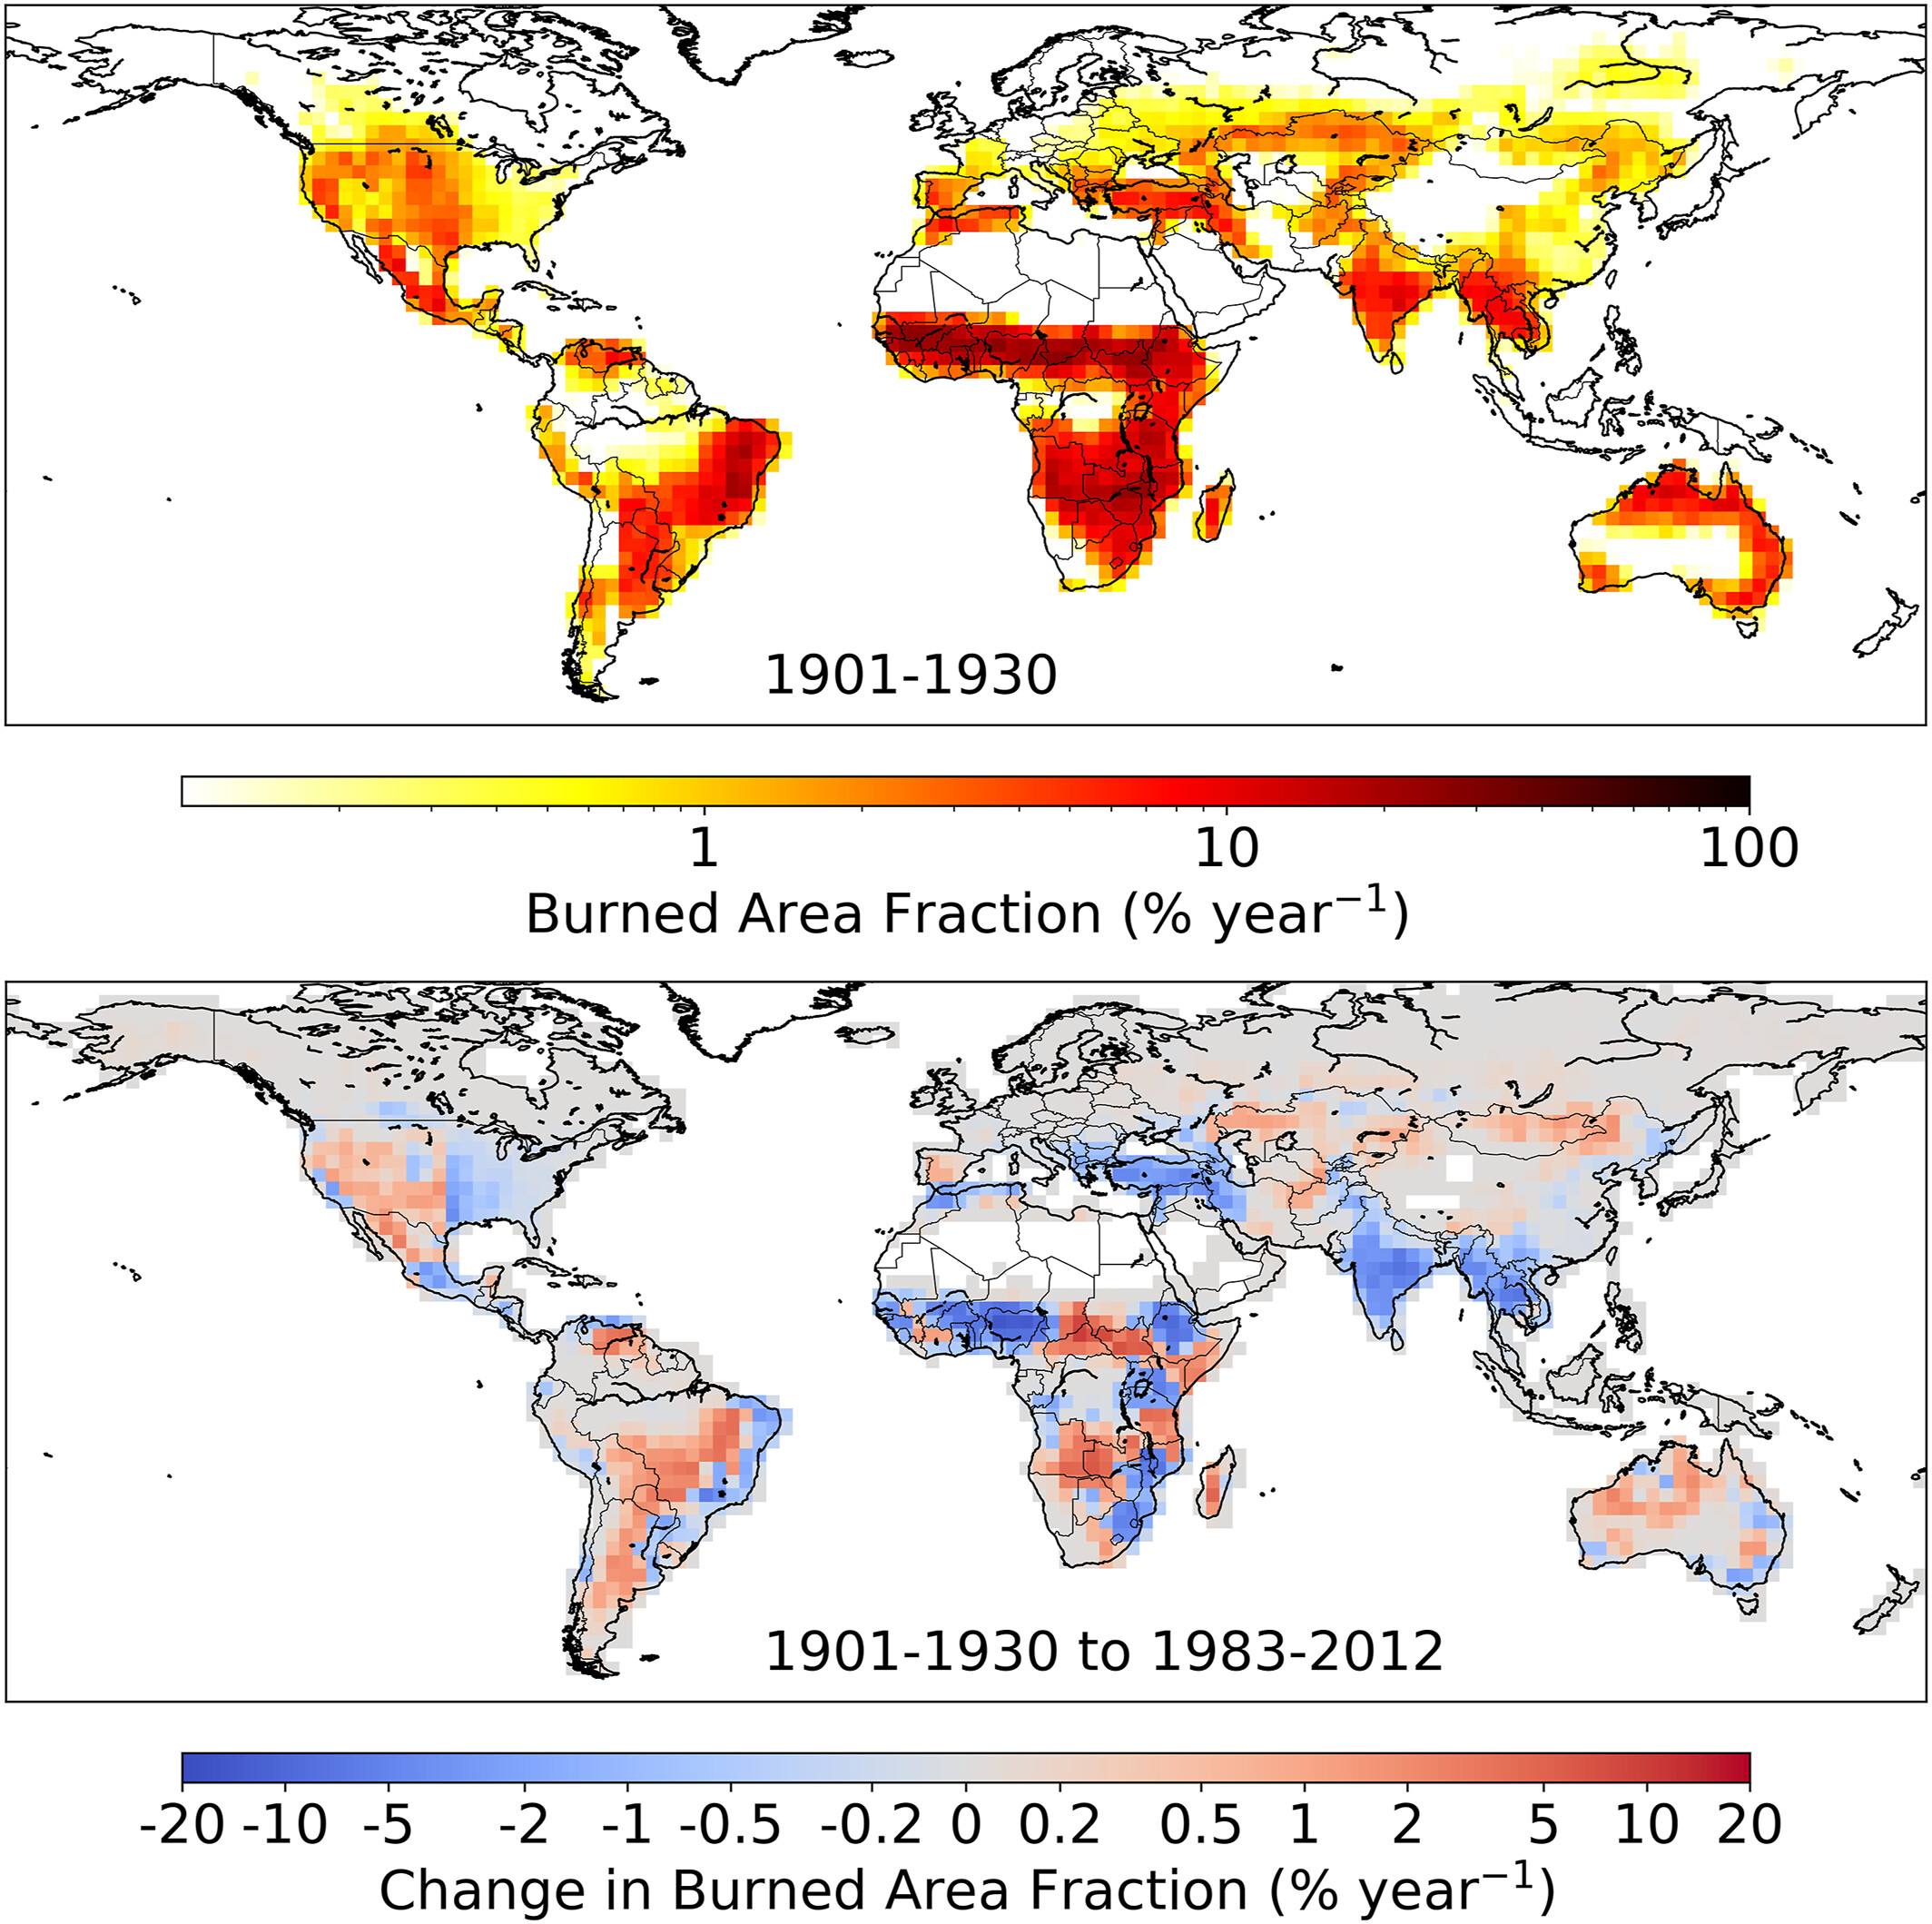
\includegraphics[width=1\linewidth]{images/burned_area_trend_1901_1930.png}
%     \caption{Multi-model median simulations of burned area (BA) fraction during 1901–1930 (\% year−1) and change in BA fraction between the periods 1901–1930 and 1983–2012 (\% year−1) from the ensemble of six Fire Model Intercomparison Project models, gridded at 2.5° resolution. (Top panel) Multi-model median estimate of mean annual BA fraction in the baseline period 1901–1930. (Right panel) Change in the multi-model median estimate of mean annual BA fraction between baseline and modern (1983–2012) periods. The model simulation data derives from Teckentrup et al. ([2019] with updates to two models after Lasslop, Hantson, Harrison, et al.  and Burton et al. ([2019]; see Text A in Supporting Information [S1].}
%     \label{fig:BA_trend_}
% \end{figure}

% \begin{figure}
%     \centering
%     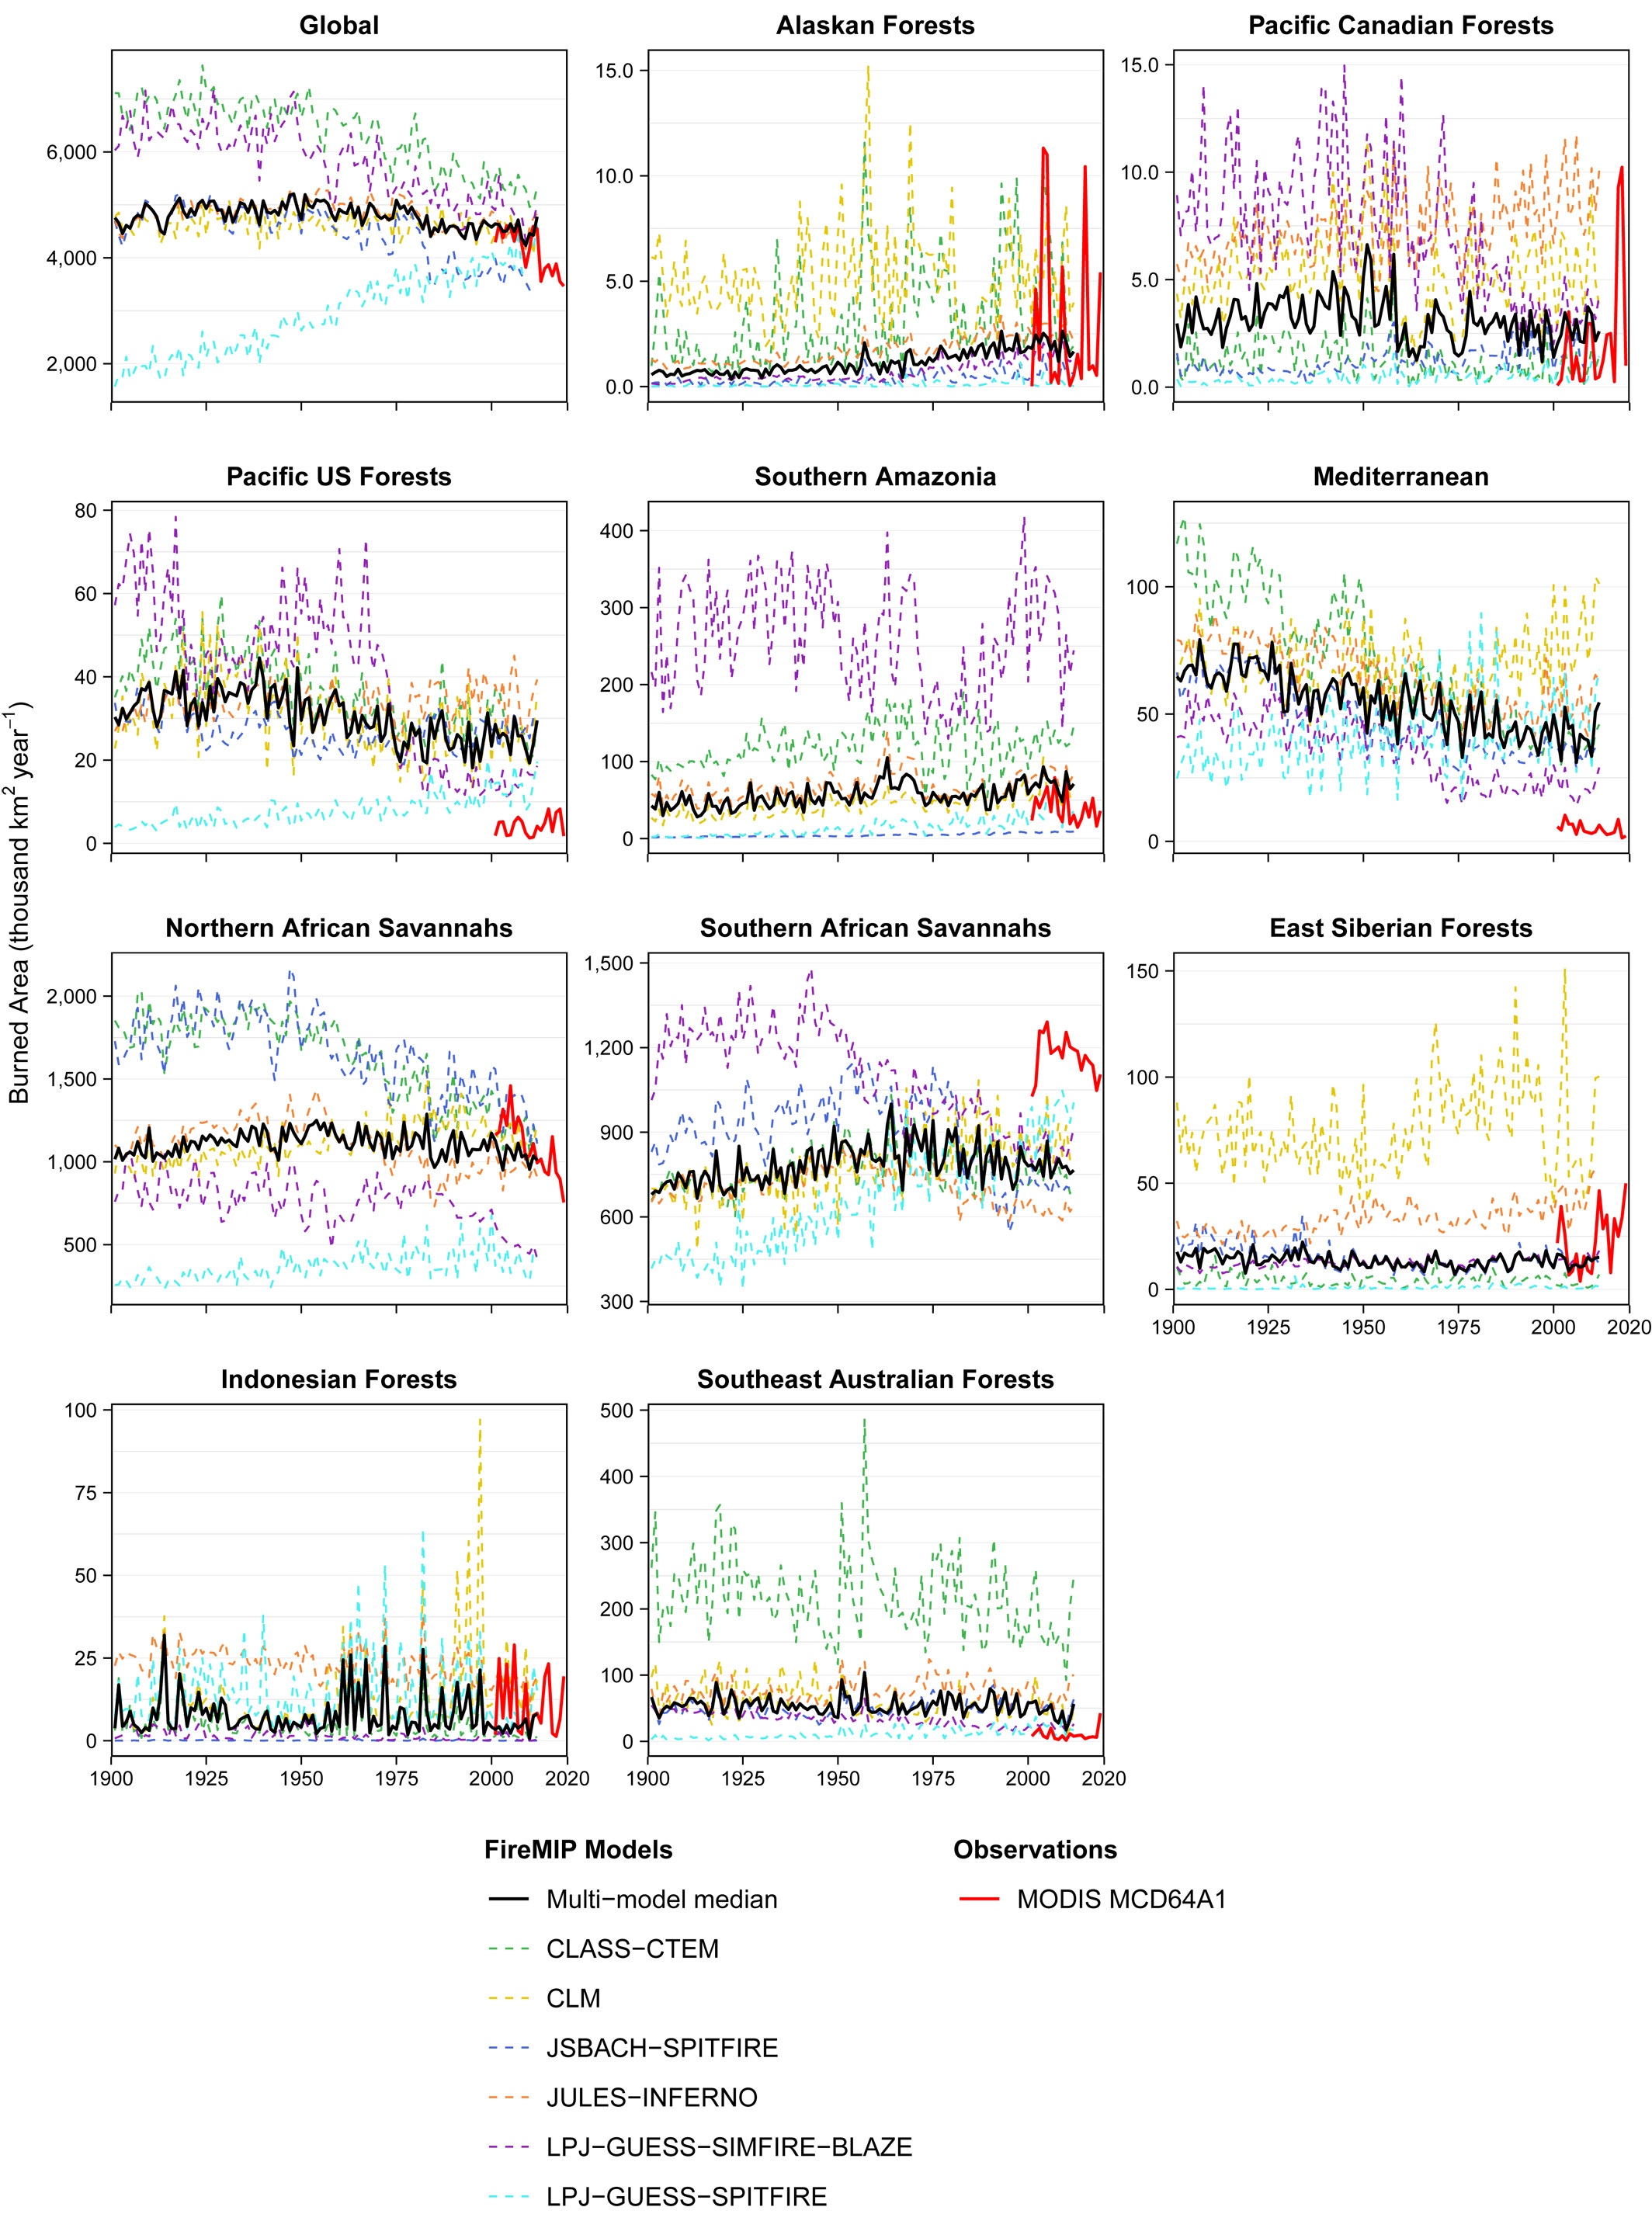
\includegraphics[width=0.8\linewidth]{images/regional_series_fireMip.png}
%     \caption{Regional time series of global and regional burned area (BA) modeled by six fire-enabled dynamic global vegetation models run offline as part of Fire Model Intercomparison Project (FireMIP) (dashed lines for individual models) (Teckentrup et al., \href{https://agupubs.onlinelibrary.wiley.com/doi/full/10.1029/2020RG000726\#rog20279-bib-0513}{2019}). The solid black lines plot the multi-model median annual BA from the FireMIP models. The solid red lines (2001–2019) plot observed BA from the moderate resolution imaging spectroradiometer BA product (Giglio et al., \href{https://agupubs.onlinelibrary.wiley.com/doi/full/10.1029/2020RG000726\#rog20279-bib-0201}{2018}). The model simulation data derives from Teckentrup et al. (\href{https://agupubs.onlinelibrary.wiley.com/doi/full/10.1029/2020RG000726\#rog20279-bib-0513}{2019}) with updates to two models after Lasslop, Hantson, Harrison, et al. (\href{https://agupubs.onlinelibrary.wiley.com/doi/full/10.1029/2020RG000726\#rog20279-bib-0309}{2020}) and Burton et al. (\href{https://agupubs.onlinelibrary.wiley.com/doi/full/10.1029/2020RG000726\#rog20279-bib-0081}{2019}; see Text A in Supporting Information \href{https://agupubs.onlinelibrary.wiley.com/doi/full/10.1029/2020RG000726\#support-information-section}{S1} for methods). }
%     \label{fig:regional_series_fireMip}
% \end{figure}

% burned Area Current trend

% \begin{figure}[H]
%     \centering
%     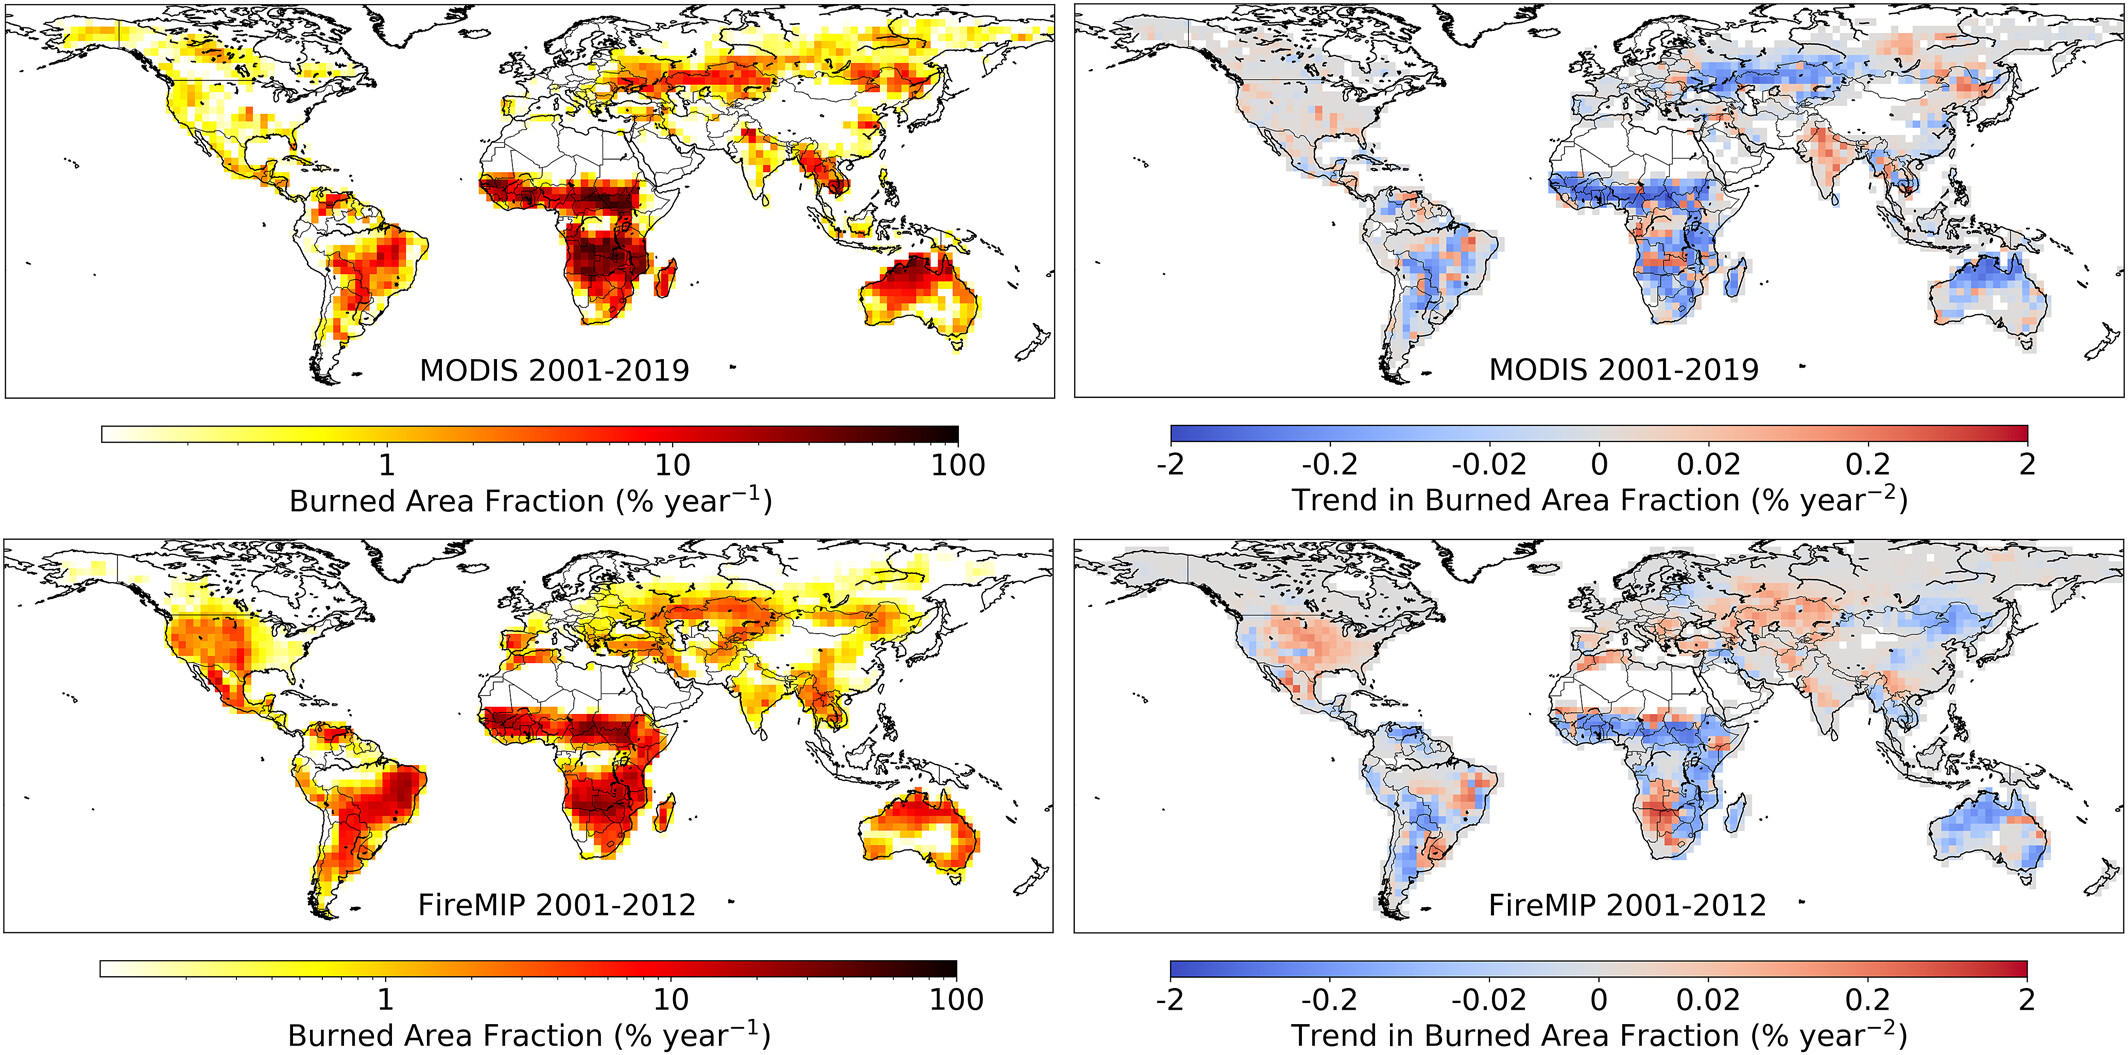
\includegraphics[width=1\linewidth]{images/BA_trend_2001_2019.png}
%     \caption{Global observed and modeled burned area (BA) fraction and their trends during the periods shown, gridded at 2.5° resolution (Giglio et al., [2018]; Teckentrup et al., [2019]. Plots show (left panels) annual mean BA fraction (\% year−1) and (right panels) trend in BA fraction (\% year−2) since 2001 period for (upper panels) moderate resolution imaging spectroradiometer BA (2001–2019) and (lower panels) six Fire Model Intercomparison Project (FireMIP) models (2001–2012). Year 2012 is the final year for which FireMIP simulations are available. The slope is calculated as the Theil-Sen estimator, which is insensitive to outliers.}
%     \label{fig:BA_trend_2001_2019}
% \end{figure}

% \begin{figure}[H]
%     \centering
%     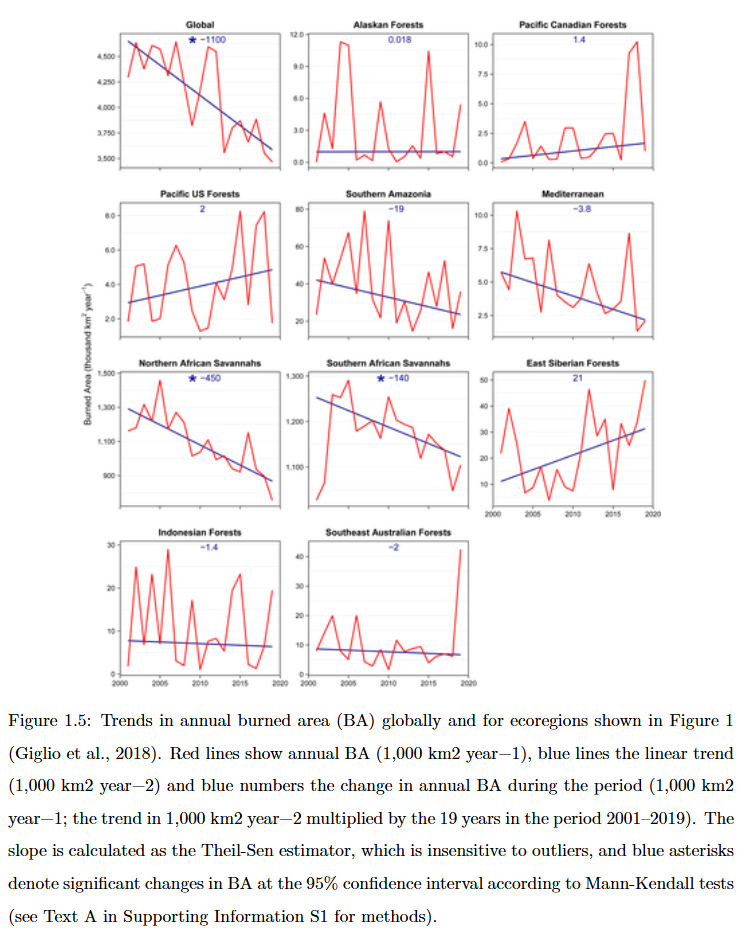
\includegraphics[width=1\linewidth]{images/BA_global_trend_regions.png}
%     \caption{Enter Caption}
%     \label{fig:BA_global_trend_regions}
% \end{figure}

% \begin{figure}[H]
%     \centering
%     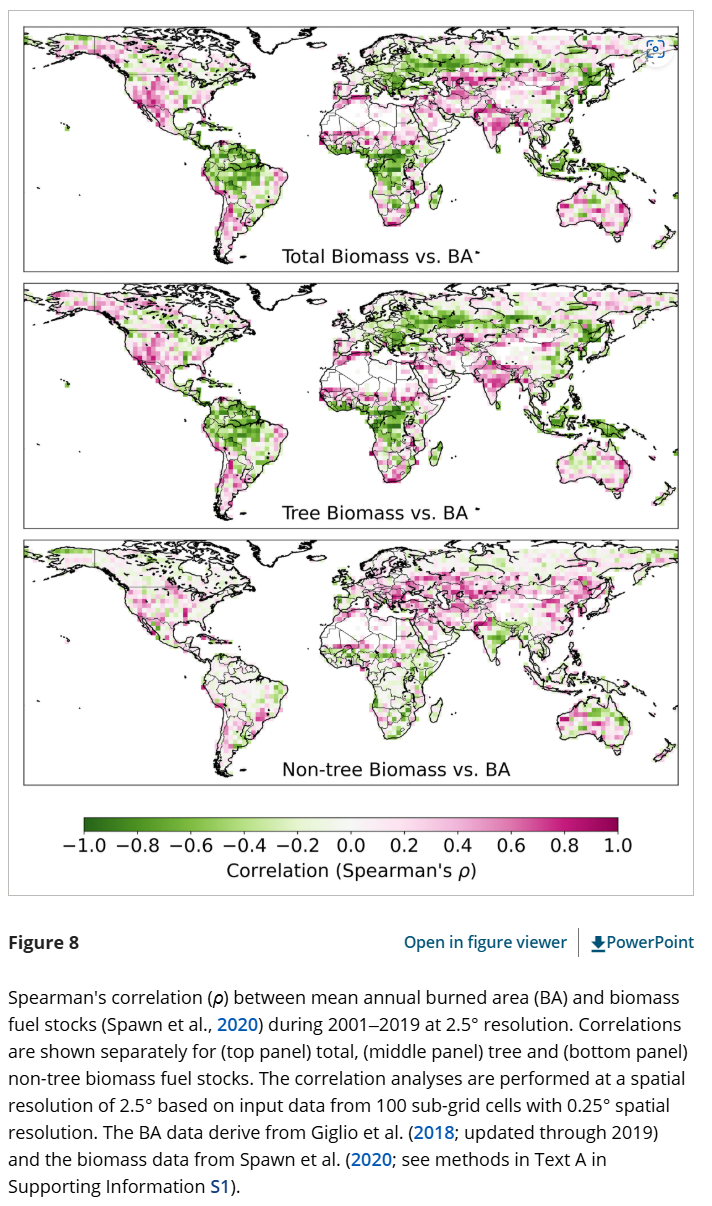
\includegraphics[width=1\linewidth]{images/map_BA_correlation_biomass_BA.png}
%     \caption{Enter Caption}
%     \label{fig:app_map_BA_correlation_biomass_BA}
% \end{figure}

% \begin{figure}[H]
%     \centering
%     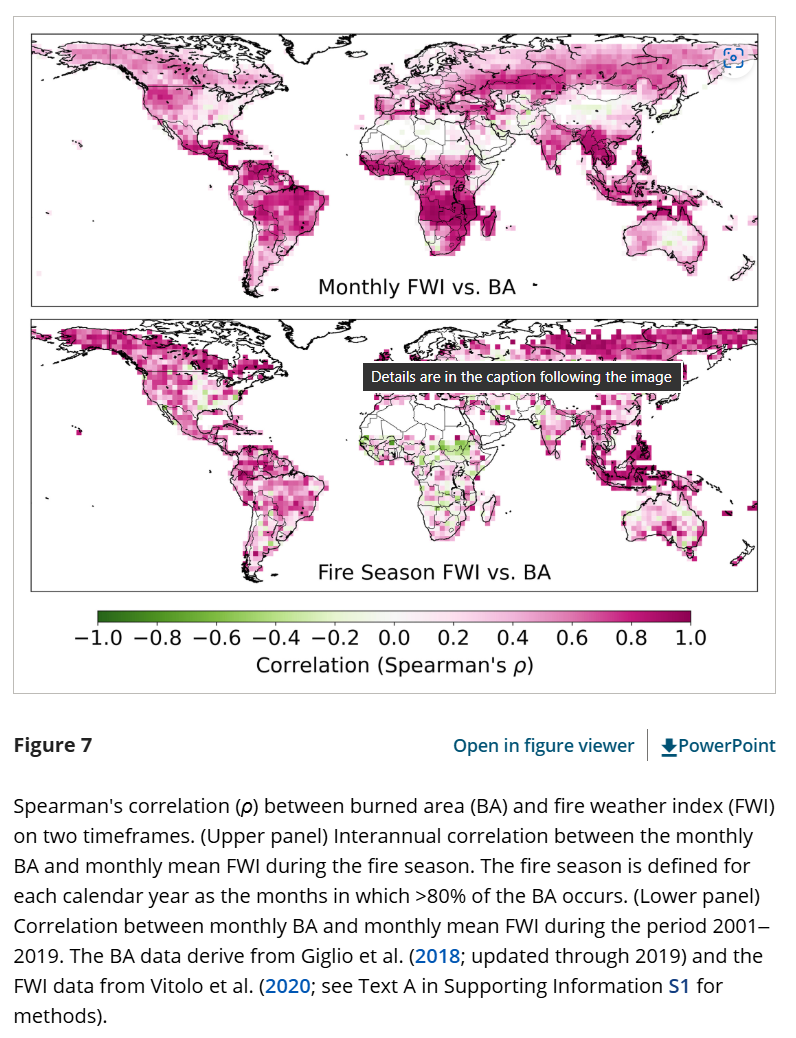
\includegraphics[width=1\linewidth]{images/map_BA_correlation_FWI.png}
%     \caption{Enter Caption}
%     \label{fig:app_map_BA_correlation_FWI}
% \end{figure}

% \begin{figure}[H]
%     \centering
%     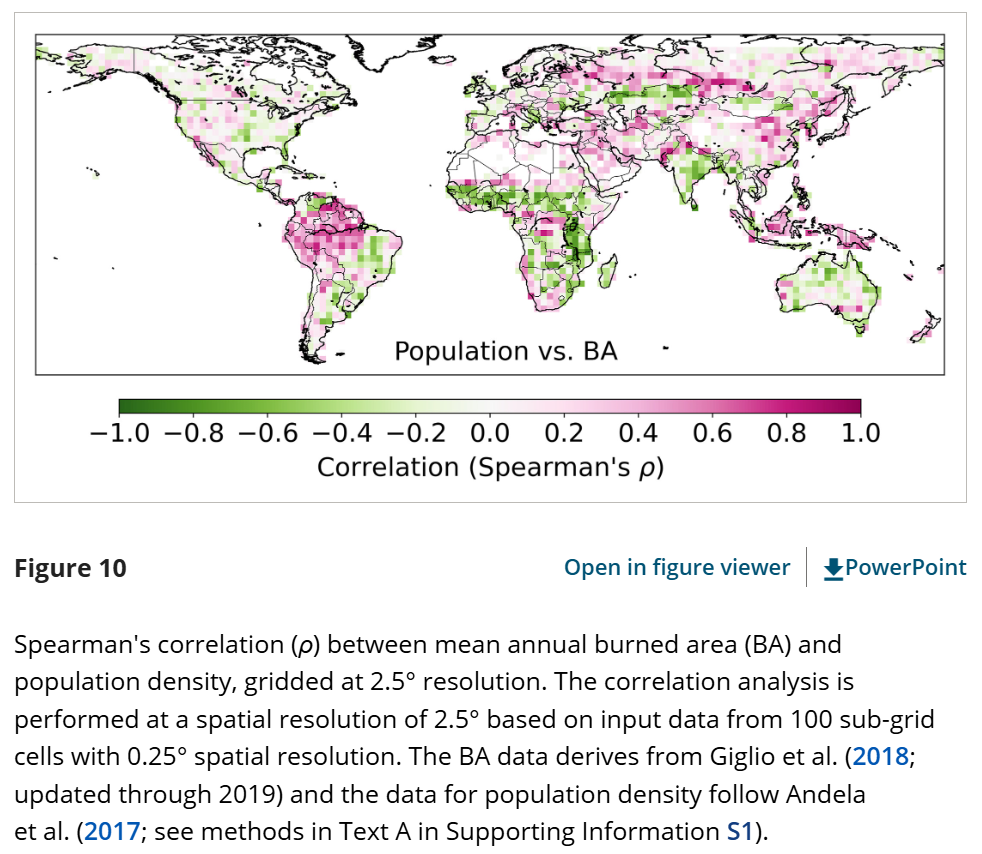
\includegraphics[width=1\linewidth]{images/map_BA_correlation_population.png}
%     \caption{Enter Caption}
%     \label{fig:app_map_BA_correlation_population}
% \end{figure}


%%% ================================================================
%%% Fire Season Maps (moved from Chapter~2)
%%% ================================================================
\section{Fire Season Maps}
\label{sec:appendix_fire_season_maps}

\begin{figure}[H]
    \centering
    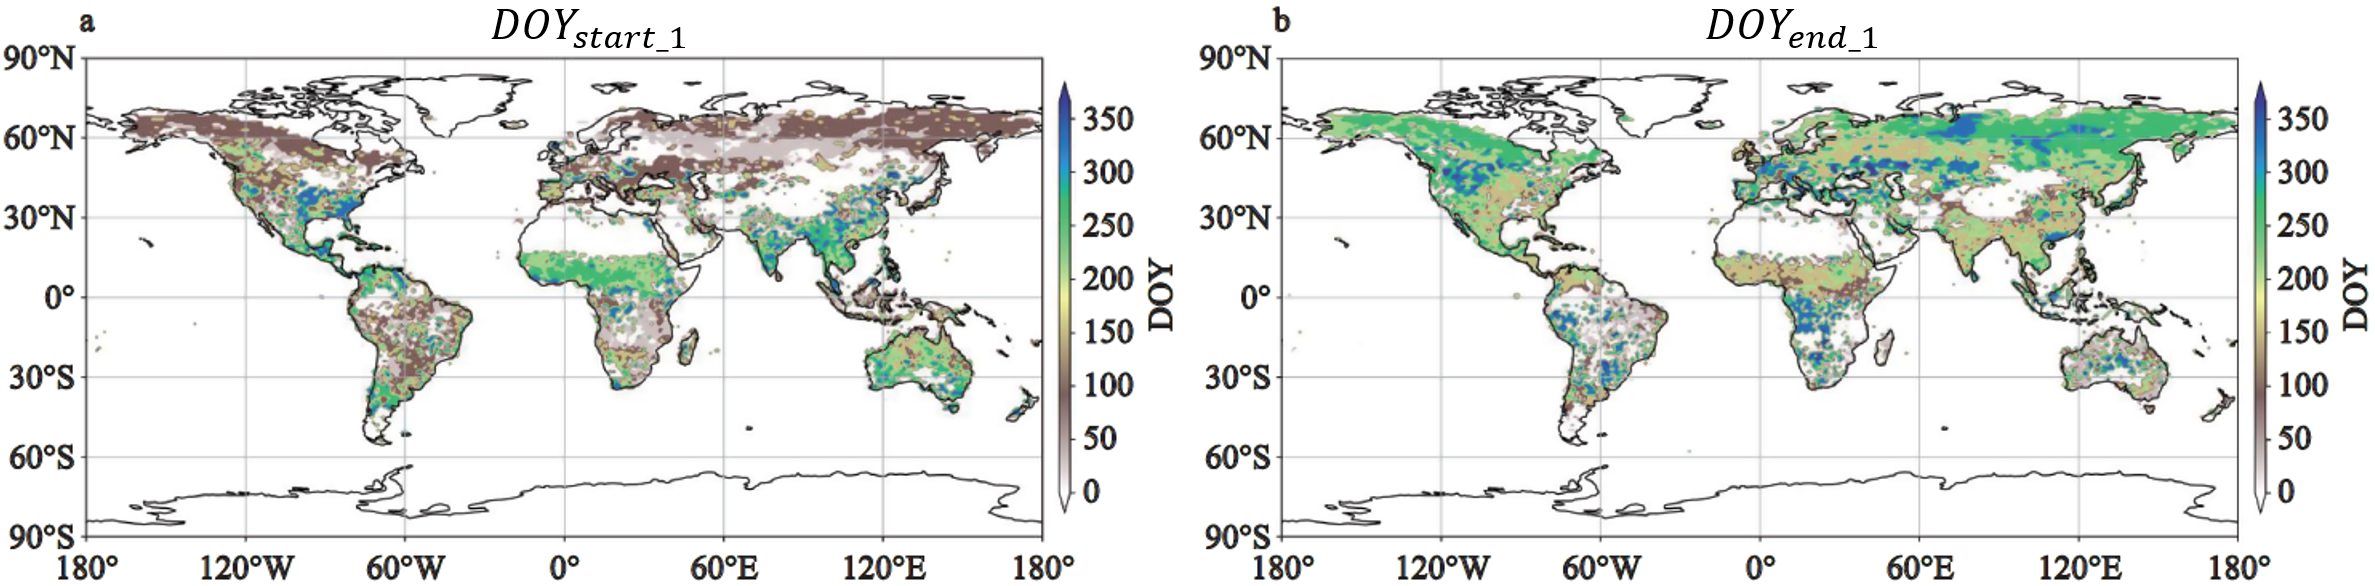
\includegraphics[width=0.9\linewidth]{images/fire_season_start1_end1.png}
    \caption{\footnotesize{Global distributions of the fire season first subperiod (see Fig. \ref{fig:fire_season_types})  start day of year $\mathrm{DOY}_{\text{start 1}}$  (a) and end $\mathrm{DOY}_{\text{end 1}}$ (b).  \textsuperscript{\ref{fn:Zhang2025}}}}
    \label{fig:fire_season_start_end}
\end{figure}

\begin{figure}[H]
    \centering
    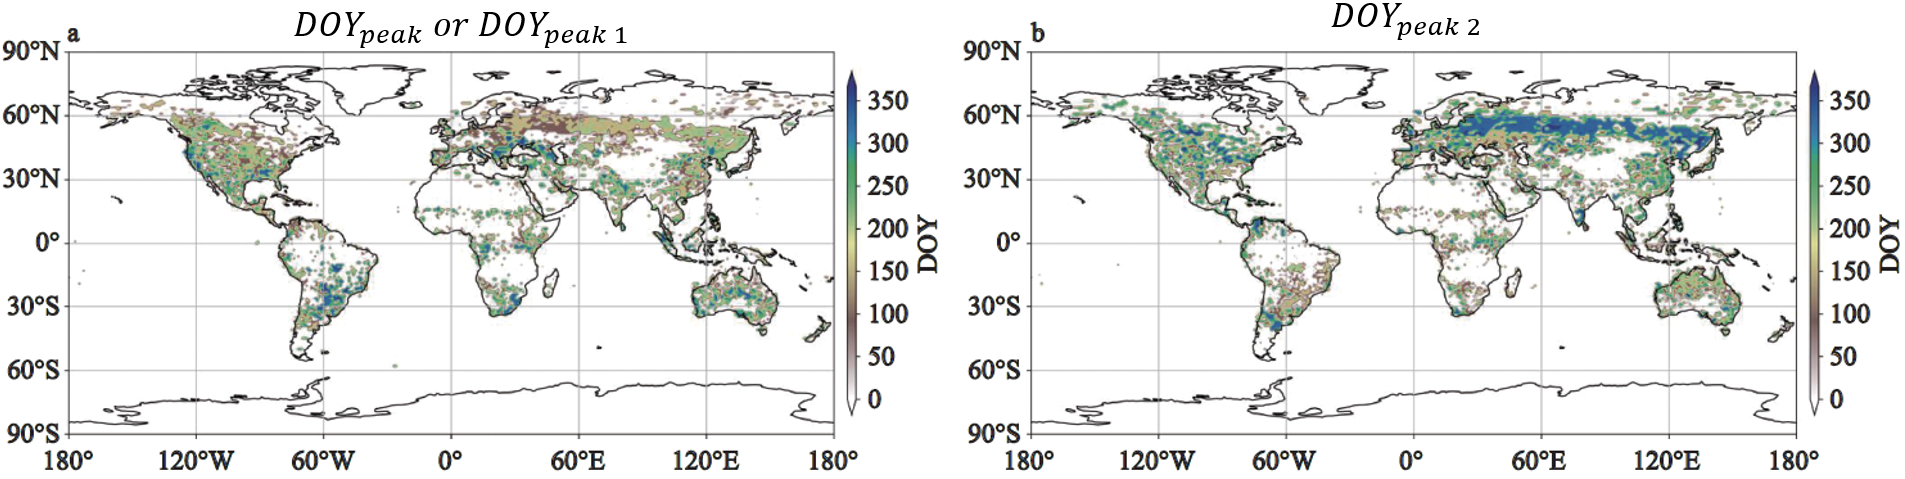
\includegraphics[width=1\linewidth]{images/fire_season_peaks.png}
    \caption{\footnotesize{Global distributions of the peak start day of year $\mathrm{DOY}_{\text{peak} 1}$ in the first subperiod (a) and second subperiod $\mathrm{DOY}_{\text{peak}  2}$(b) of fire season from 2001 to 2022. See Fig.~\ref{fig:fire_season_types} for subperiod definitions.  \textsuperscript{\ref{fn:Zhang2025}}}}
    \label{fig:fire_season_peaks}
\end{figure}

\begin{figure}[H]
    \centering
    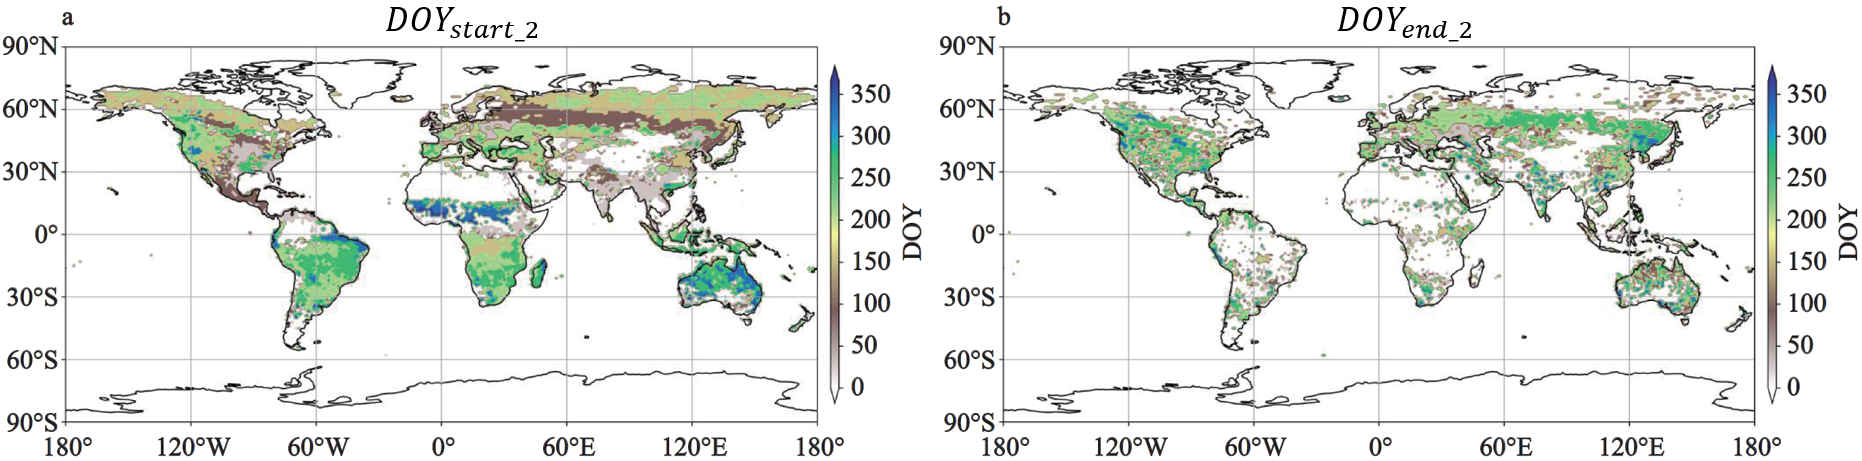
\includegraphics[width=1\linewidth]{images/fire_season_start2_end2.png}
    \caption{\footnotesize{Global distributions of the fire season second subperiod start day of year $\mathrm{DOY}_{\text{start 2}}$ (a) and end $\mathrm{DOY}_{\text{end 2}}$ (b); see Fig.~\ref{fig:fire_season_types} for subperiod definitions.  \textsuperscript{\ref{fn:Zhang2025}}}}
    \label{fig:fire_season_start2_end2}
\end{figure}


%%% ================================================================
%%% Baseline FPR Coverage Maps (moved from Chapter~\ref{chapter-9-the-proposed-system-concept})
%%% ================================================================
\section{$\mathcal{C}_{\text{Zoom}}$ Baseline FPR Coverage Maps ($\eta = 65^{\circ}$)}
\label{sec:appendix_zoom_baseline_fpr}

The following baseline ($\eta = 65^{\circ}$) maps complement the combined recurrent-and-occasional
map retained in Section~\ref{sec:fpr_temporal_coverage_baseline}.

\begin{figure}[H]
    \centering
    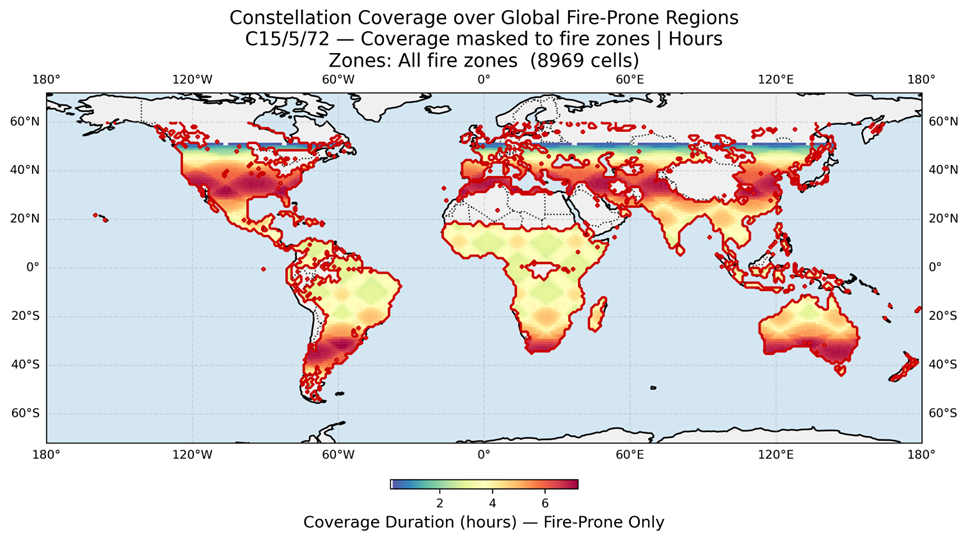
\includegraphics[width=1\linewidth]{images/c_zoom_global_FRP_bondaries_Tcoverage_eta63.png}
    \caption{\footnotesize{Temporal coverage~$T_{\text{cov}}$ of the FPR boundaries mask for $\mathcal{C}_{\text{Zoom}}$ at the baseline $\eta = 65^{\circ}$.  The boundaries mask encompasses all fire-prone cells regardless of recurrence group, showing the full geographic extent monitored by the constellation.}}
    \label{fig:c_zoom_global_FRP_bondaries_Tcoverage_eta63}
\end{figure}

\begin{figure}[H]
    \centering
    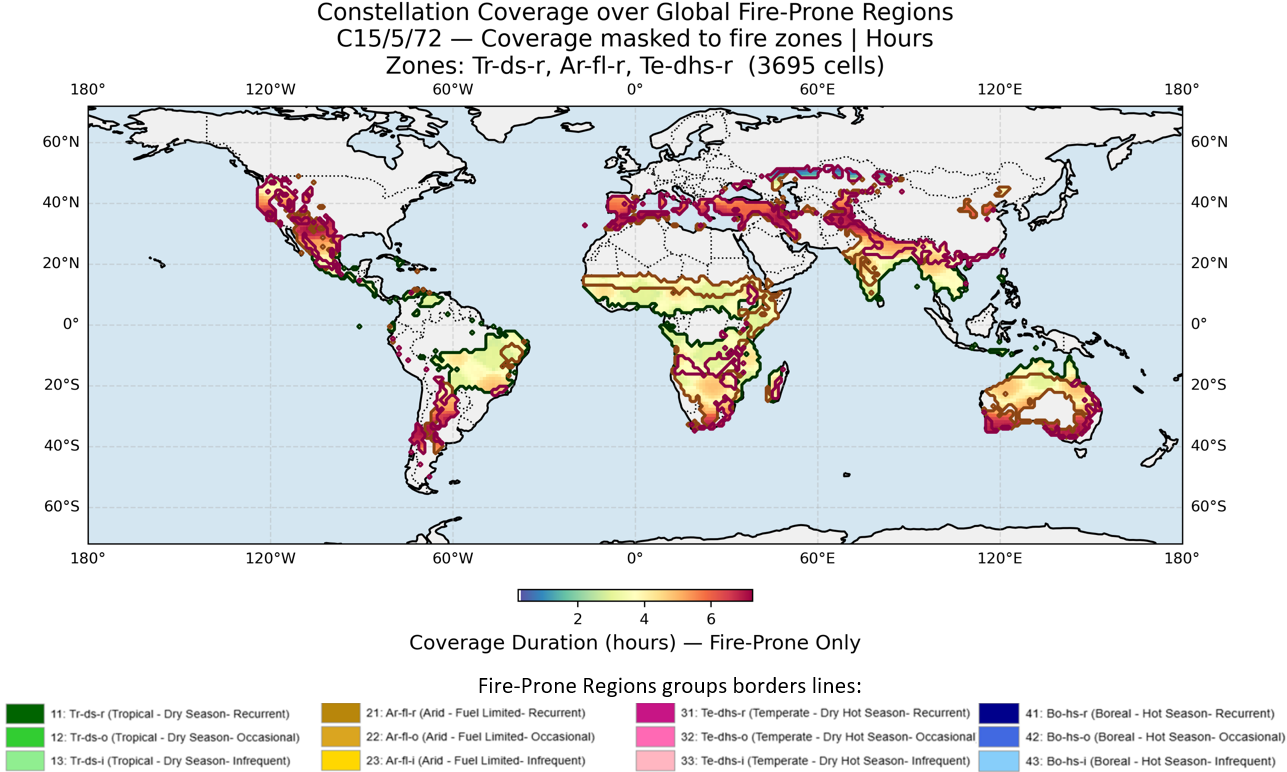
\includegraphics[width=1\linewidth]{images/c_zoom_global_FRP_recurrent_Tcoverage_eta63.png}
    \caption{\footnotesize{Temporal coverage~$T_{\text{cov}}$ of the recurrent-only FPR mask for $\mathcal{C}_{\text{Zoom}}$ at the baseline $\eta = 65^{\circ}$.  Only cells classified as recurrent ($r$, ${>}\,7$~fires/decade) are shown, highlighting the temperate and Mediterranean forest biomes near $\phi \approx \pm\,40^{\circ}$ that constitute the highest-priority monitoring targets.}}
    \label{fig:c_zoom_global_FRP_recurrent_Tcoverage_eta63}
\end{figure}


%%% ================================================================
%%% 7-Day RGTO Seed Propagation Maps (moved from Chapter~8)
%%% ================================================================
\section{7-Day RGTO Seed Propagation Maps}
\label{sec:appendix_7day_maps}

\begin{figure}[H]
    \centering
    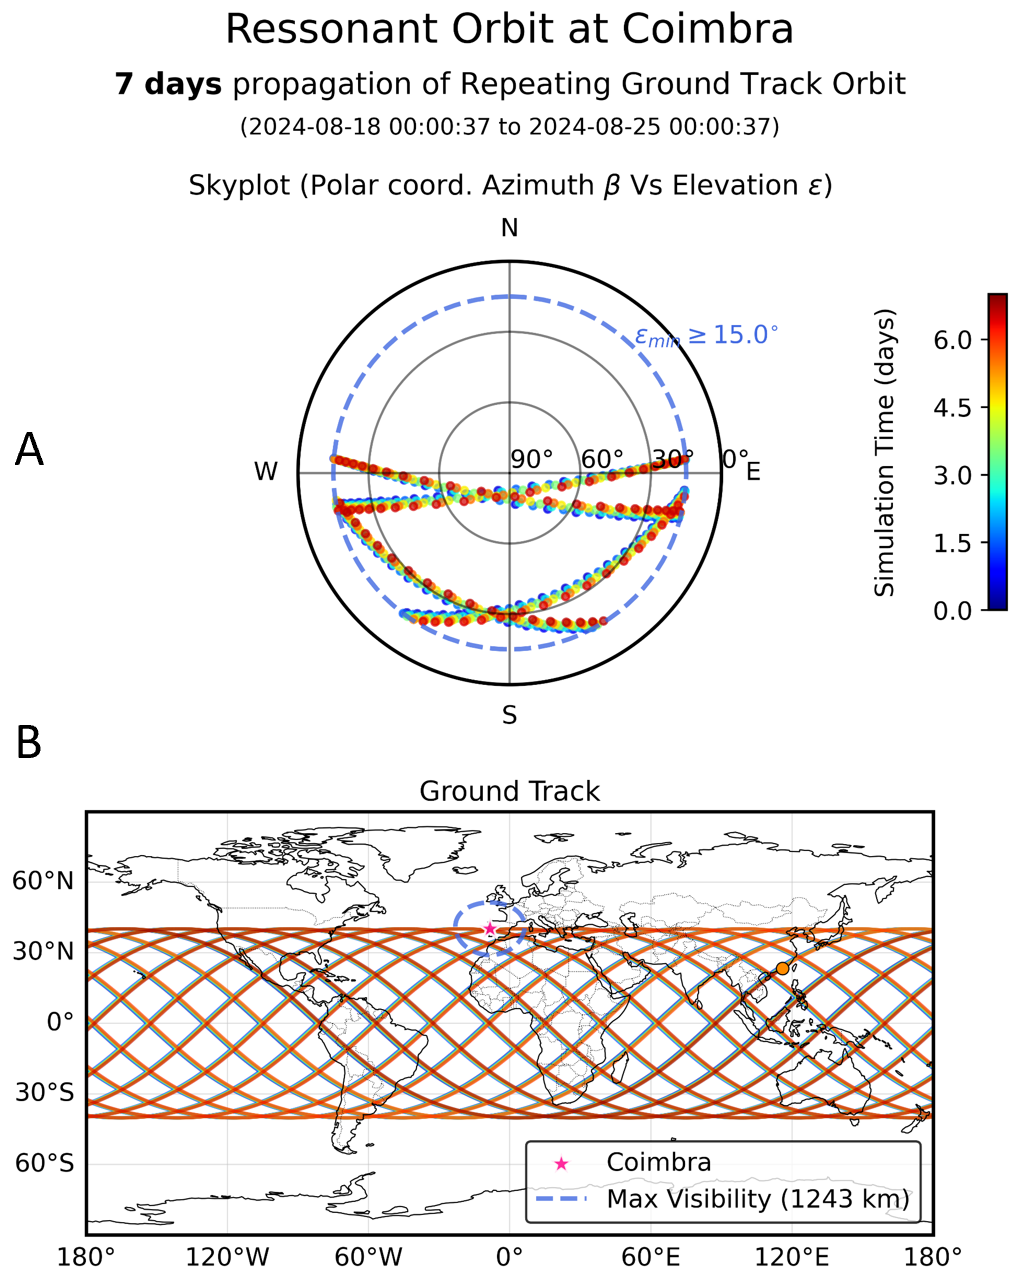
\includegraphics[width=0.8\linewidth]{images/RGTO_maps_Coimbra_Seven_days.png}
    \caption{\footnotesize{7-day RGTO seed propagation over Coimbra without station-keeping ($\tau=15/1$, $h \approx 488$\,km, $i=40.2^{\circ}$).  \textbf{(A)}~Sky plot showing the recurring four-pass cluster with consistent azimuth--elevation trajectories across all seven days.  \textbf{(B)}~Ground track; the trace overlaps the 1-day pattern (Fig.~\ref{fig:RGTO_maps_Coimbra_One_day}), confirming short-term resonance stability under drag and $J_{8\times8}$ perturbations.}}
    \label{fig:RGTO_maps_Coimbra_Seven_days}
\end{figure}


%%% ================================================================
%%% Walker Constellation Example (moved from Chapter~8)
%%% ================================================================
\section{Walker Constellation Illustration}
\label{sec:appendix_walker_example}

\begin{figure}[H]
    \centering
    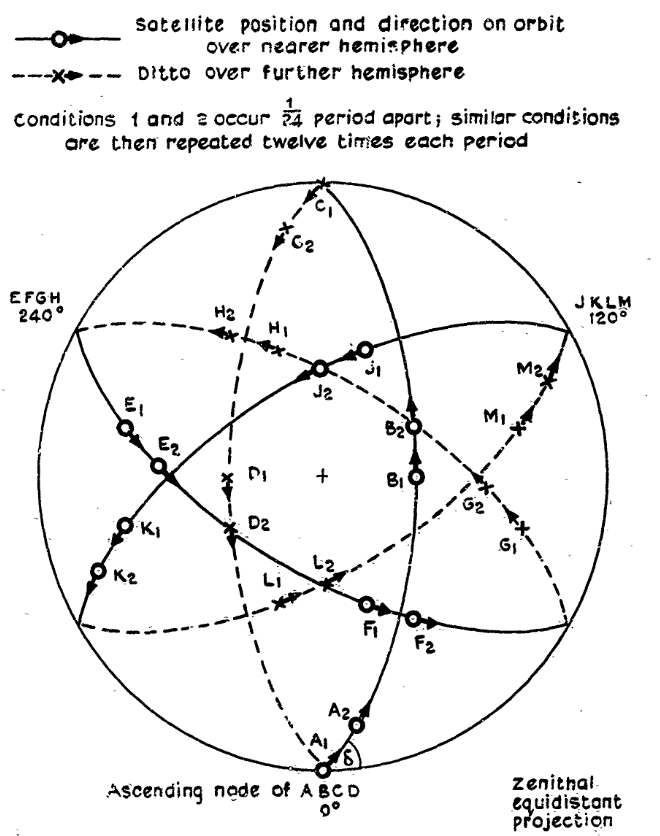
\includegraphics[width=0.4\linewidth]{images/constellation_walker_12_sats_3planes_ example.png}
    \caption{\footnotesize{Walker-$\delta$ constellation example: 12 satellites distributed across 3 orbital planes ($\mathcal{C}_{12/3/120}$), shown in a polar zenithal equidistant projection with the ascending node at the equator as the reference ($\mathrm{RAAN}_{\mathrm{ref}}=0^{\circ}$).  Each plane carries four satellites uniformly phased in true anomaly; the inter-plane RAAN spacing is $120^{\circ}$.  This projection framework is adopted throughout the constellation design \cite{walker_circular_1970}.}}
    \label{fig:constellation_walker_12_sats_3planes_ example}
\end{figure}


%%% ================================================================
%%% 4-Plane Observation Links (moved from Chapter~8)
%%% ================================================================
\section{Four-Plane Constellation Observation Links}
\label{sec:appendix_4plane_obs}

\begin{figure}[H]
    \centering
    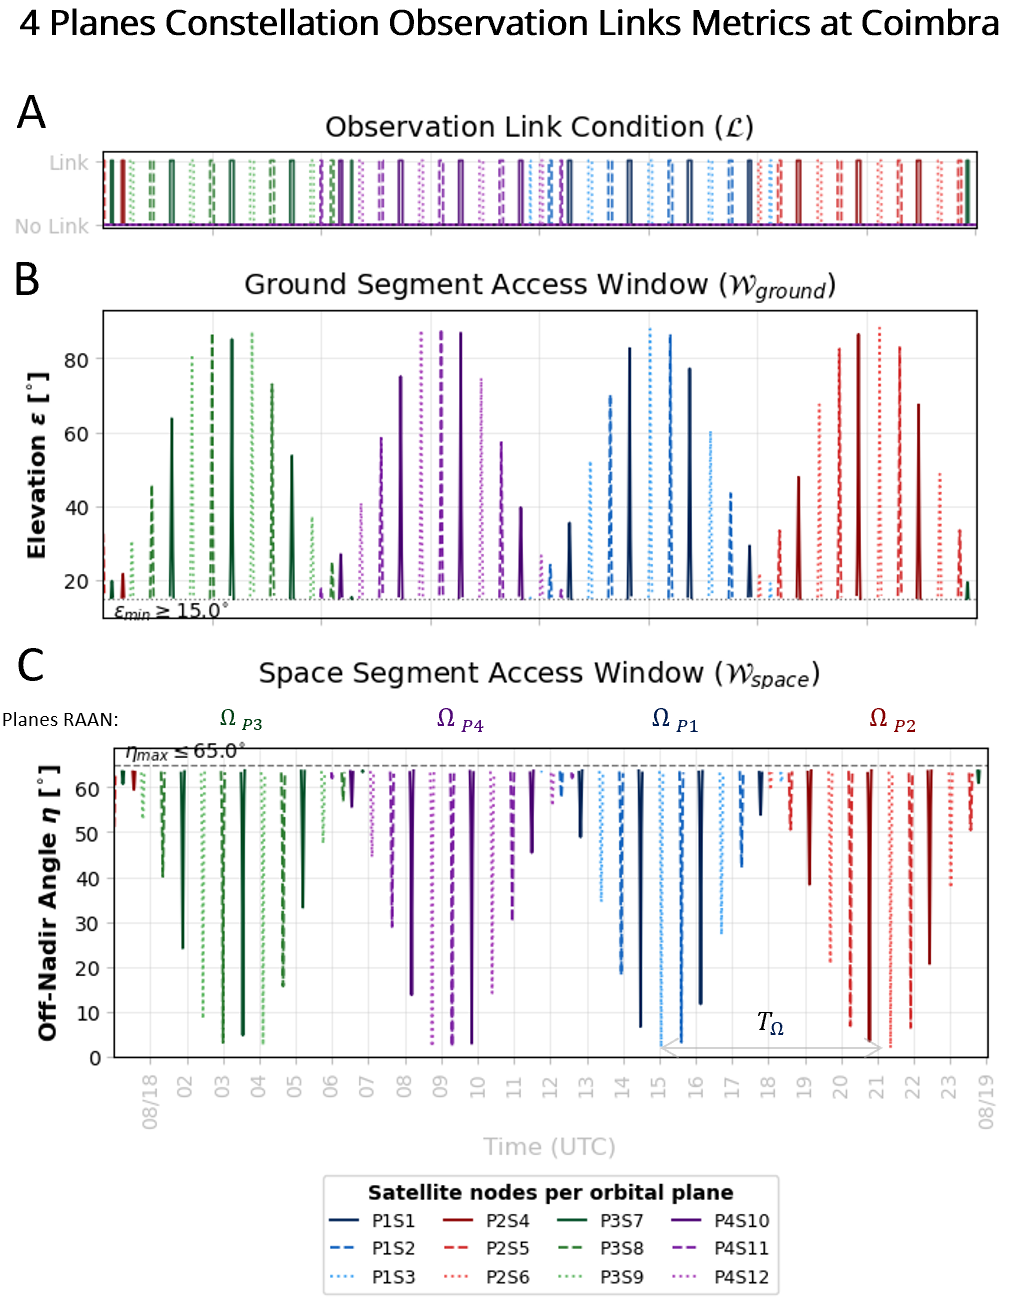
\includegraphics[width=0.95\linewidth]{images/4_planes_Constellation_Observation_Links_at_Coimbra.png}
    \caption{\footnotesize{Observation links at Coimbra for a 4-plane Walker RGTO constellation $\mathcal{C}_{12/4/90}$ derived from $T_{\mathrm{seq,max}} \approx 364.5$\,min.  The inter-plane RAAN spacing is $\delta\Omega = 90^{\circ}$, giving $\Omega_{P1}=100^{\circ}$, $\Omega_{P2}=190^{\circ}$, $\Omega_{P3}=280^{\circ}$, $\Omega_{P4}=10^{\circ}$.  Each plane contributes four high-quality near-nadir passes per day; however, visible gaps between consecutive plane windows indicate insufficient temporal uniformity for the 30-minute monitoring requirement.}}
    \label{fig:obs_links_4planes}
\end{figure}


%%% Zoom Layer η-Sweep Figures (from Chapter~\ref{chapter-9-the-proposed-system-concept})
%%% ================================================================
\section{$\mathcal{C}_{\text{Zoom}}$ Off-Nadir Angle Sweep Maps}
\label{sec:appendix_zoom_eta_sweep}

The following figures complement the baseline ($\eta = 65^{\circ}$) results presented in
Section~\ref{sec:zoom_layer} by showing the temporal-coverage maps for reduced off-nadir
angle configurations ($\eta = 45^{\circ}$, $30^{\circ}$, $15^{\circ}$).

%%% --- Global Temporal Coverage ---
\subsection{Global Domain Temporal Coverage}

\begin{figure}[H]
    \centering
    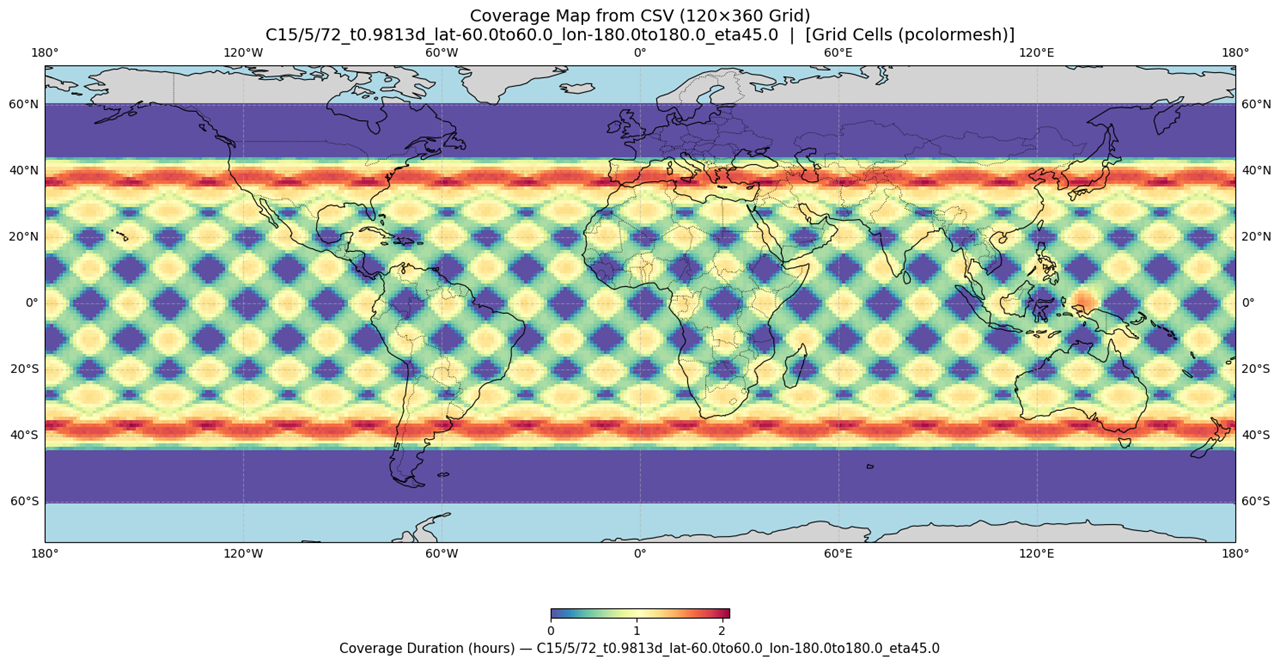
\includegraphics[width=1\linewidth]{images/c_zoom_global_Tcoverage_eta45.png}
    \caption{\footnotesize{Global temporal coverage map for $\eta = 45^{\circ}$.}}
    \label{fig:c_zoom_global_Tcoverage_eta45}
\end{figure}

\begin{figure}[H]
    \centering
    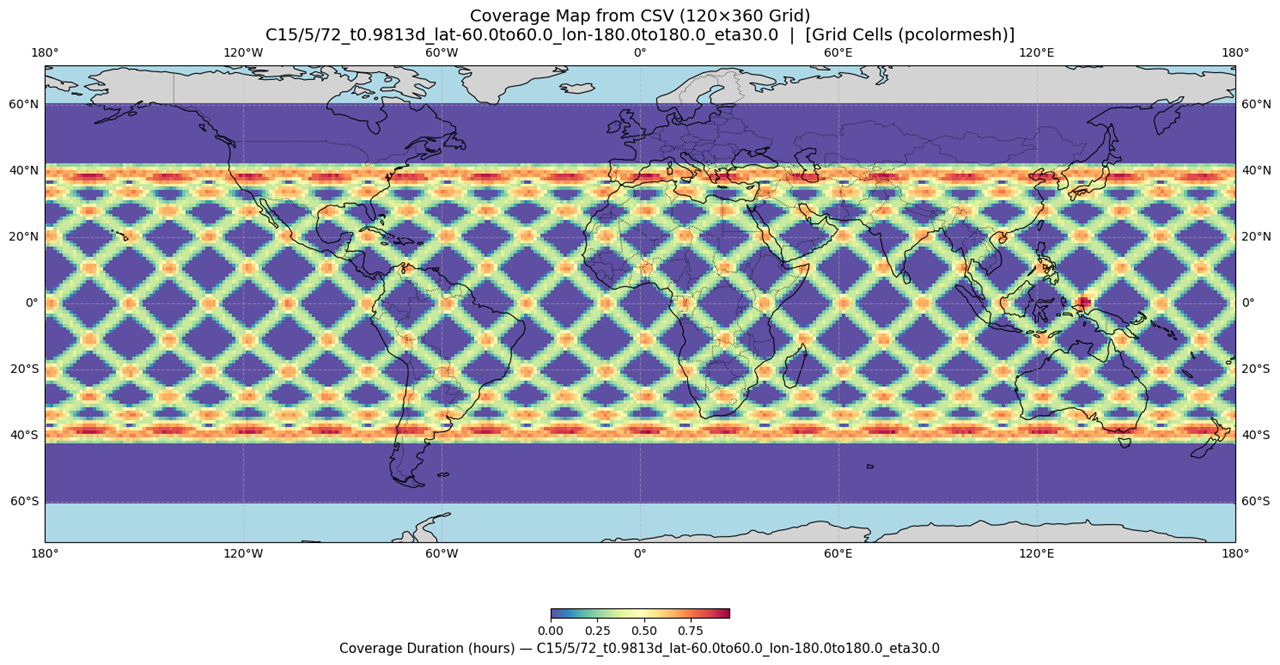
\includegraphics[width=1\linewidth]{images/c_zoom_global_Tcoverage_eta30.png}
    \caption{\footnotesize{Global temporal coverage map for $\eta = 30^{\circ}$.}}
    \label{fig:c_zoom_global_Tcoverage_eta30}
\end{figure}

\begin{figure}[H]
    \centering
    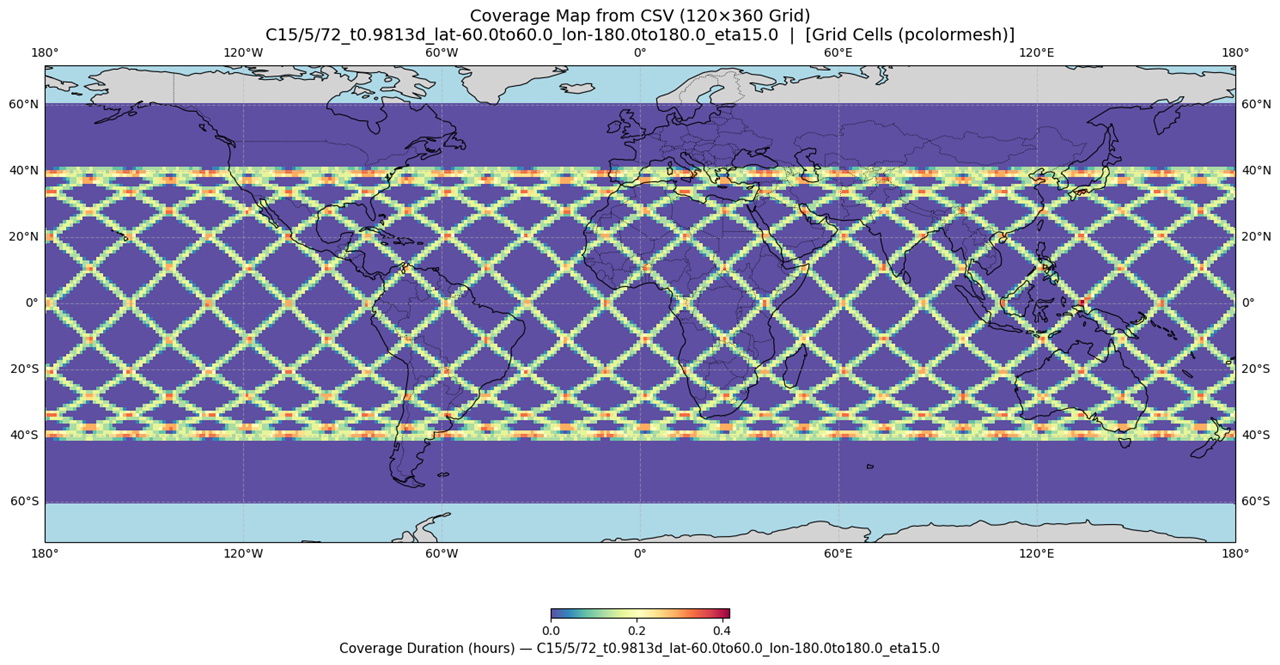
\includegraphics[width=1\linewidth]{images/c_zoom_global_Tcoverage_eta15.png}
    \caption{\footnotesize{Global temporal coverage map for $\eta = 15^{\circ}$.}}
    \label{fig:c_zoom_global_Tcoverage_eta15}
\end{figure}

%%% --- FPR Boundaries ---
\subsection{Fire-Prone Region Boundaries Temporal Coverage}

\begin{figure}[H]
    \centering
    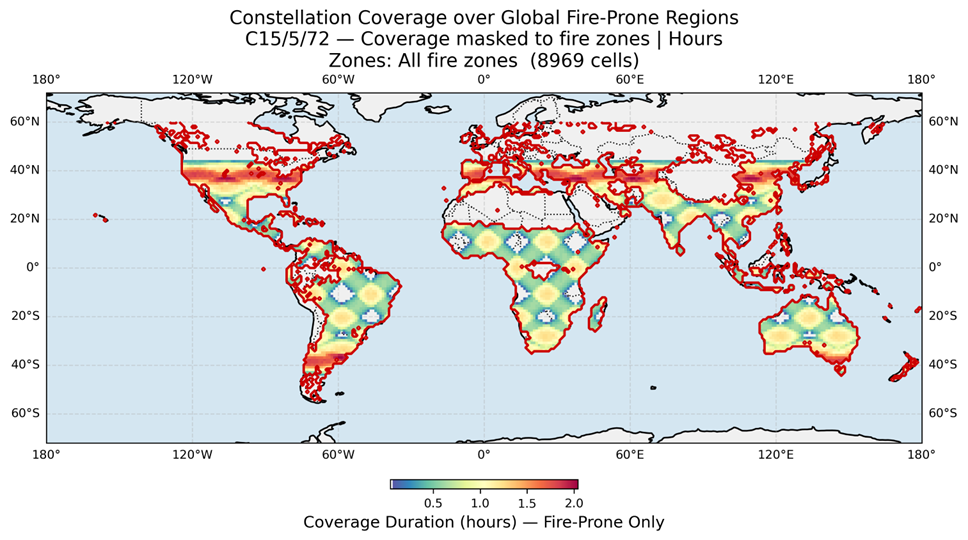
\includegraphics[width=1\linewidth]{images/c_zoom_global_FRP_boundaries_Tcoverage_eta45.png}
    \caption{\footnotesize{FPR boundaries temporal coverage for $\eta = 45^{\circ}$.}}
    \label{fig:c_zoom_global_FRP_boundaries_Tcoverage_eta45}
\end{figure}

\begin{figure}[H]
    \centering
    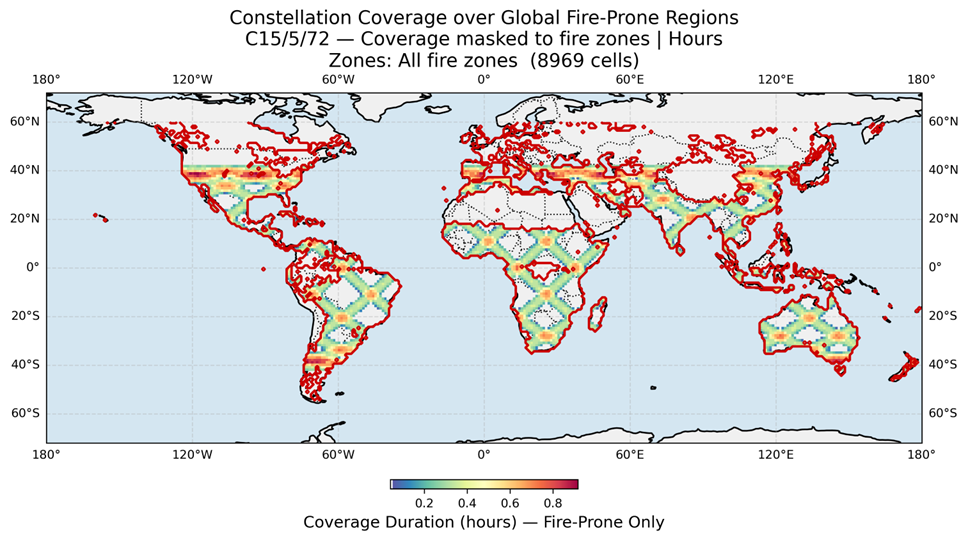
\includegraphics[width=1\linewidth]{images/c_zoom_global_FRP_boundaries_Tcoverage_eta30.png}
    \caption{\footnotesize{FPR boundaries temporal coverage for $\eta = 30^{\circ}$.}}
    \label{fig:c_zoom_global_FRP_boundaries_Tcoverage_eta30}
\end{figure}

\begin{figure}[H]
    \centering
    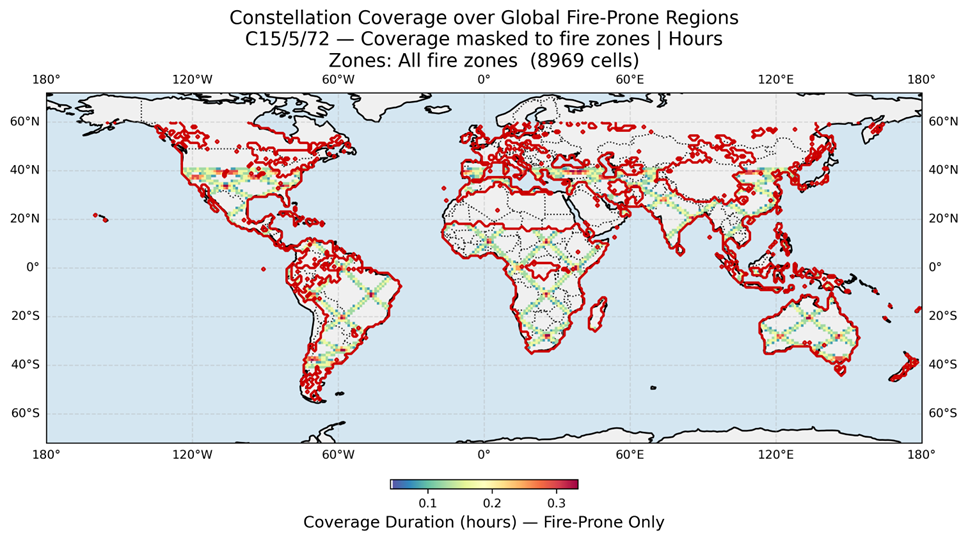
\includegraphics[width=1\linewidth]{images/c_zoom_global_FPR_boundaries_Tcoverage_eta15.png}
    \caption{\footnotesize{FPR boundaries temporal coverage for $\eta = 15^{\circ}$.}}
    \label{fig:c_zoom_global_FPR_boundaries_Tcoverage_eta15}
\end{figure}

%%% --- FPR Recurrent ---
\subsection{Recurrent Fire-Prone Region Temporal Coverage}

\begin{figure}[H]
    \centering
    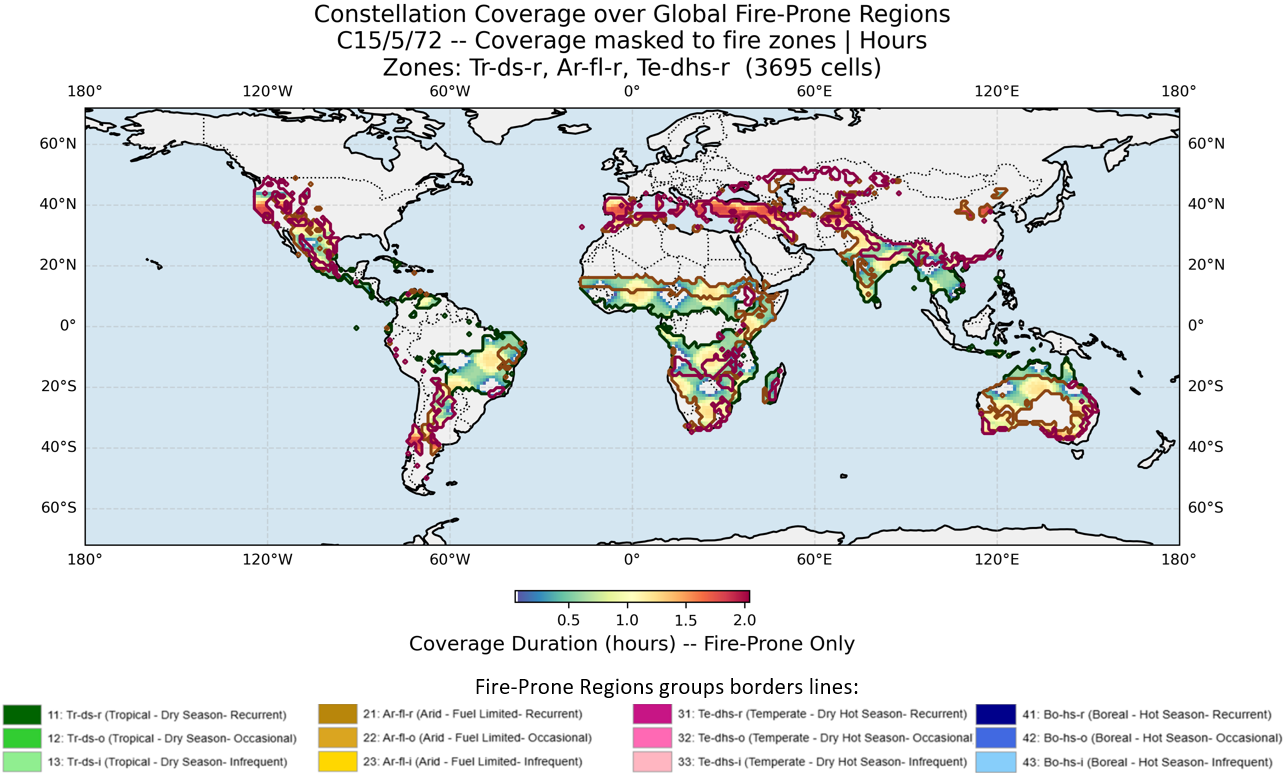
\includegraphics[width=1\linewidth]{images/c_zoom_global_FRP_recurrent_Tcoverage_eta45.png}
    \caption{\footnotesize{Recurrent FPR temporal coverage for $\eta = 45^{\circ}$.}}
    \label{fig:c_zoom_global_FRP_recurrent_Tcoverage_eta45}
\end{figure}

\begin{figure}[H]
    \centering
    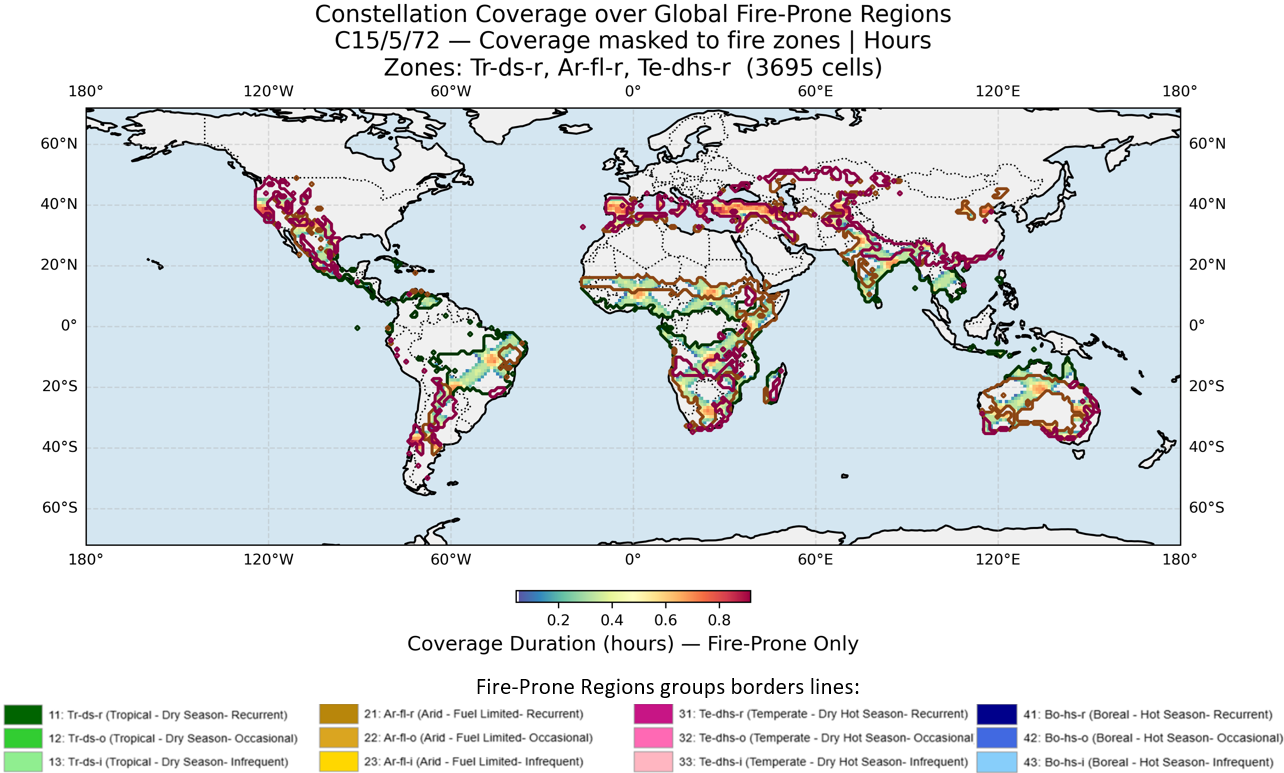
\includegraphics[width=1\linewidth]{images/c_zoom_global_FRP_recurrent_Tcoverage_eta30.png}
    \caption{\footnotesize{Recurrent FPR temporal coverage for $\eta = 30^{\circ}$.}}
    \label{fig:c_zoom_global_FRP_recurrent_Tcoverage_eta30}
\end{figure}

\begin{figure}[H]
    \centering
    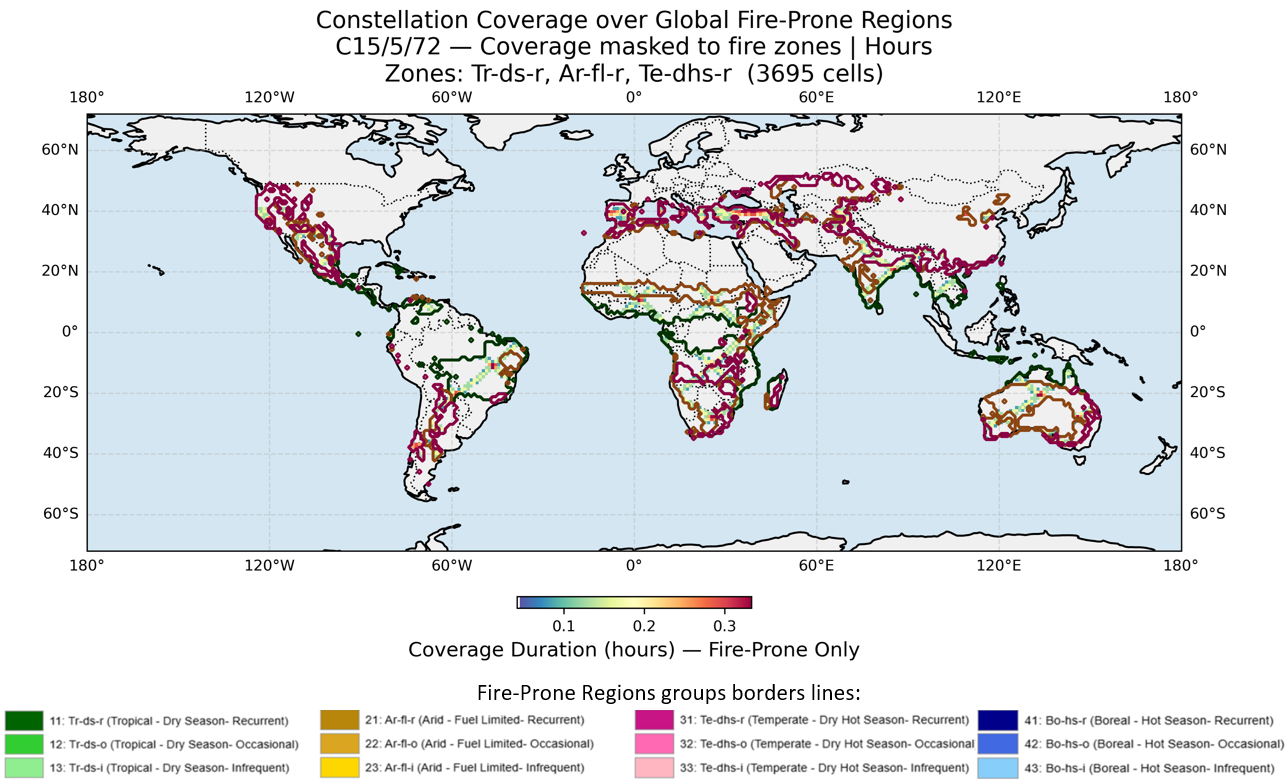
\includegraphics[width=1\linewidth]{images/c_zoom_global_FRP_recurrent_Tcoverage_eta15.png}
    \caption{\footnotesize{Recurrent FPR temporal coverage for $\eta = 15^{\circ}$.}}
    \label{fig:c_zoom_global_FRP_recurrent_Tcoverage_eta15}
\end{figure}

%%% --- FPR Recurrent + Occasional ---
\subsection{Recurrent and Occasional Fire-Prone Region Temporal Coverage}

\begin{figure}[H]
    \centering
    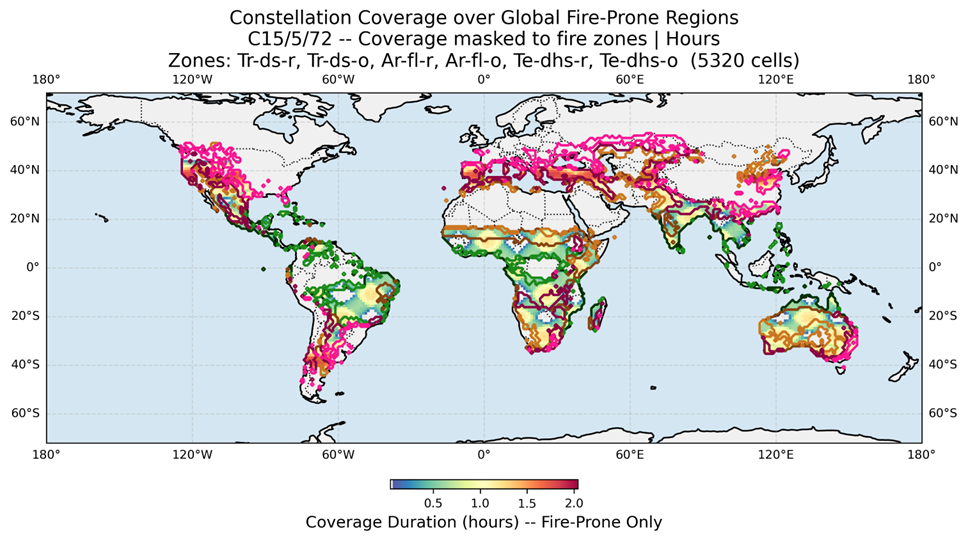
\includegraphics[width=1\linewidth]{images/c_zoom_global_FPR_recurrent_ocasional_Tcoverage_eta45.png}
    \caption{\footnotesize{Recurrent and occasional FPR temporal coverage for $\eta = 45^{\circ}$.}}
    \label{fig:c_zoom_global_FPR_recurrent_ocasional_Tcoverage_eta45}
\end{figure}

\begin{figure}[H]
    \centering
    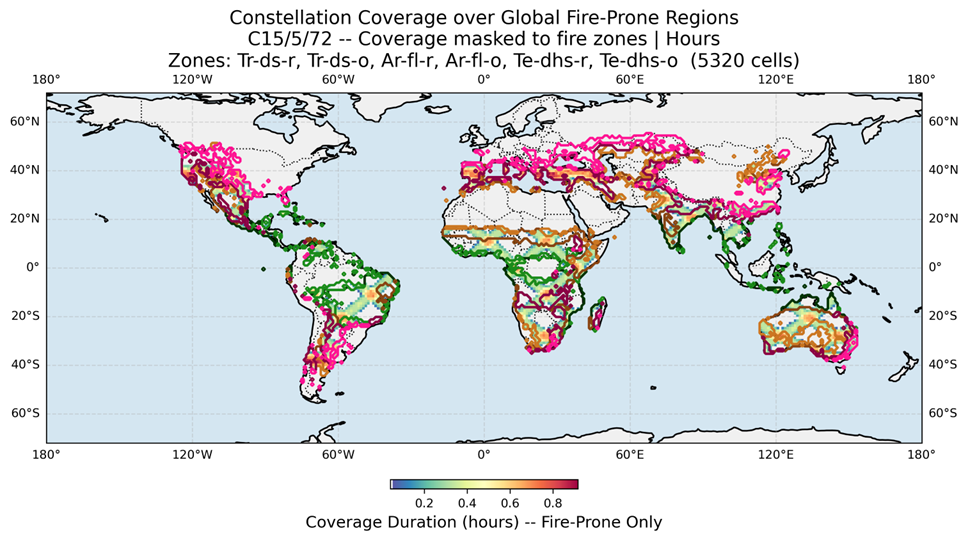
\includegraphics[width=1\linewidth]{images/c_zoom_global_FPR_recurrent_ocasional_Tcoverage_eta30.png}
    \caption{\footnotesize{Recurrent and occasional FPR temporal coverage for $\eta = 30^{\circ}$.}}
    \label{fig:c_zoom_global_FPR_recurrent_ocasional_Tcoverage_eta30}
\end{figure}

\begin{figure}[H]
    \centering
    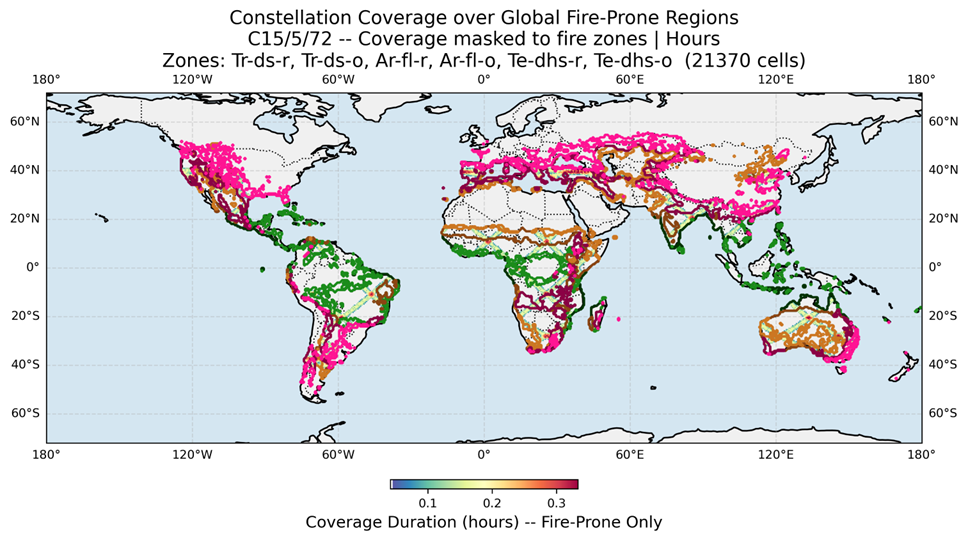
\includegraphics[width=1\linewidth]{images/c_zoom_global_FPR_recurrent_ocasional_Tcoverage_eta15.png}
    \caption{\footnotesize{Recurrent and occasional FPR temporal coverage for $\eta = 15^{\circ}$.}}
    \label{fig:c_zoom_global_FPR_recurrent_ocasional_Tcoverage_eta15}
\end{figure}


%%% ================================================================
%%% FPR Coverage Statistics and Latitude Profile
%%% ================================================================
\section{$\mathcal{C}_{\text{Zoom}}$ FPR Coverage Statistics and Latitude Profile}
\label{sec:appendix_zoom_fpr_statistics}

The following figures provide the detailed bar-chart, scatter-plot, and latitude-profile
breakdowns of the five performance variables across FPR recurrence groups and $\eta$
configurations, complementing the spatial coverage maps in
Section~\ref{sec:global_Domain_fire_prone_regions_statistics}.

\begin{landscape}

%%% --- Normalised ---
\begin{figure}[H]
    \centering
    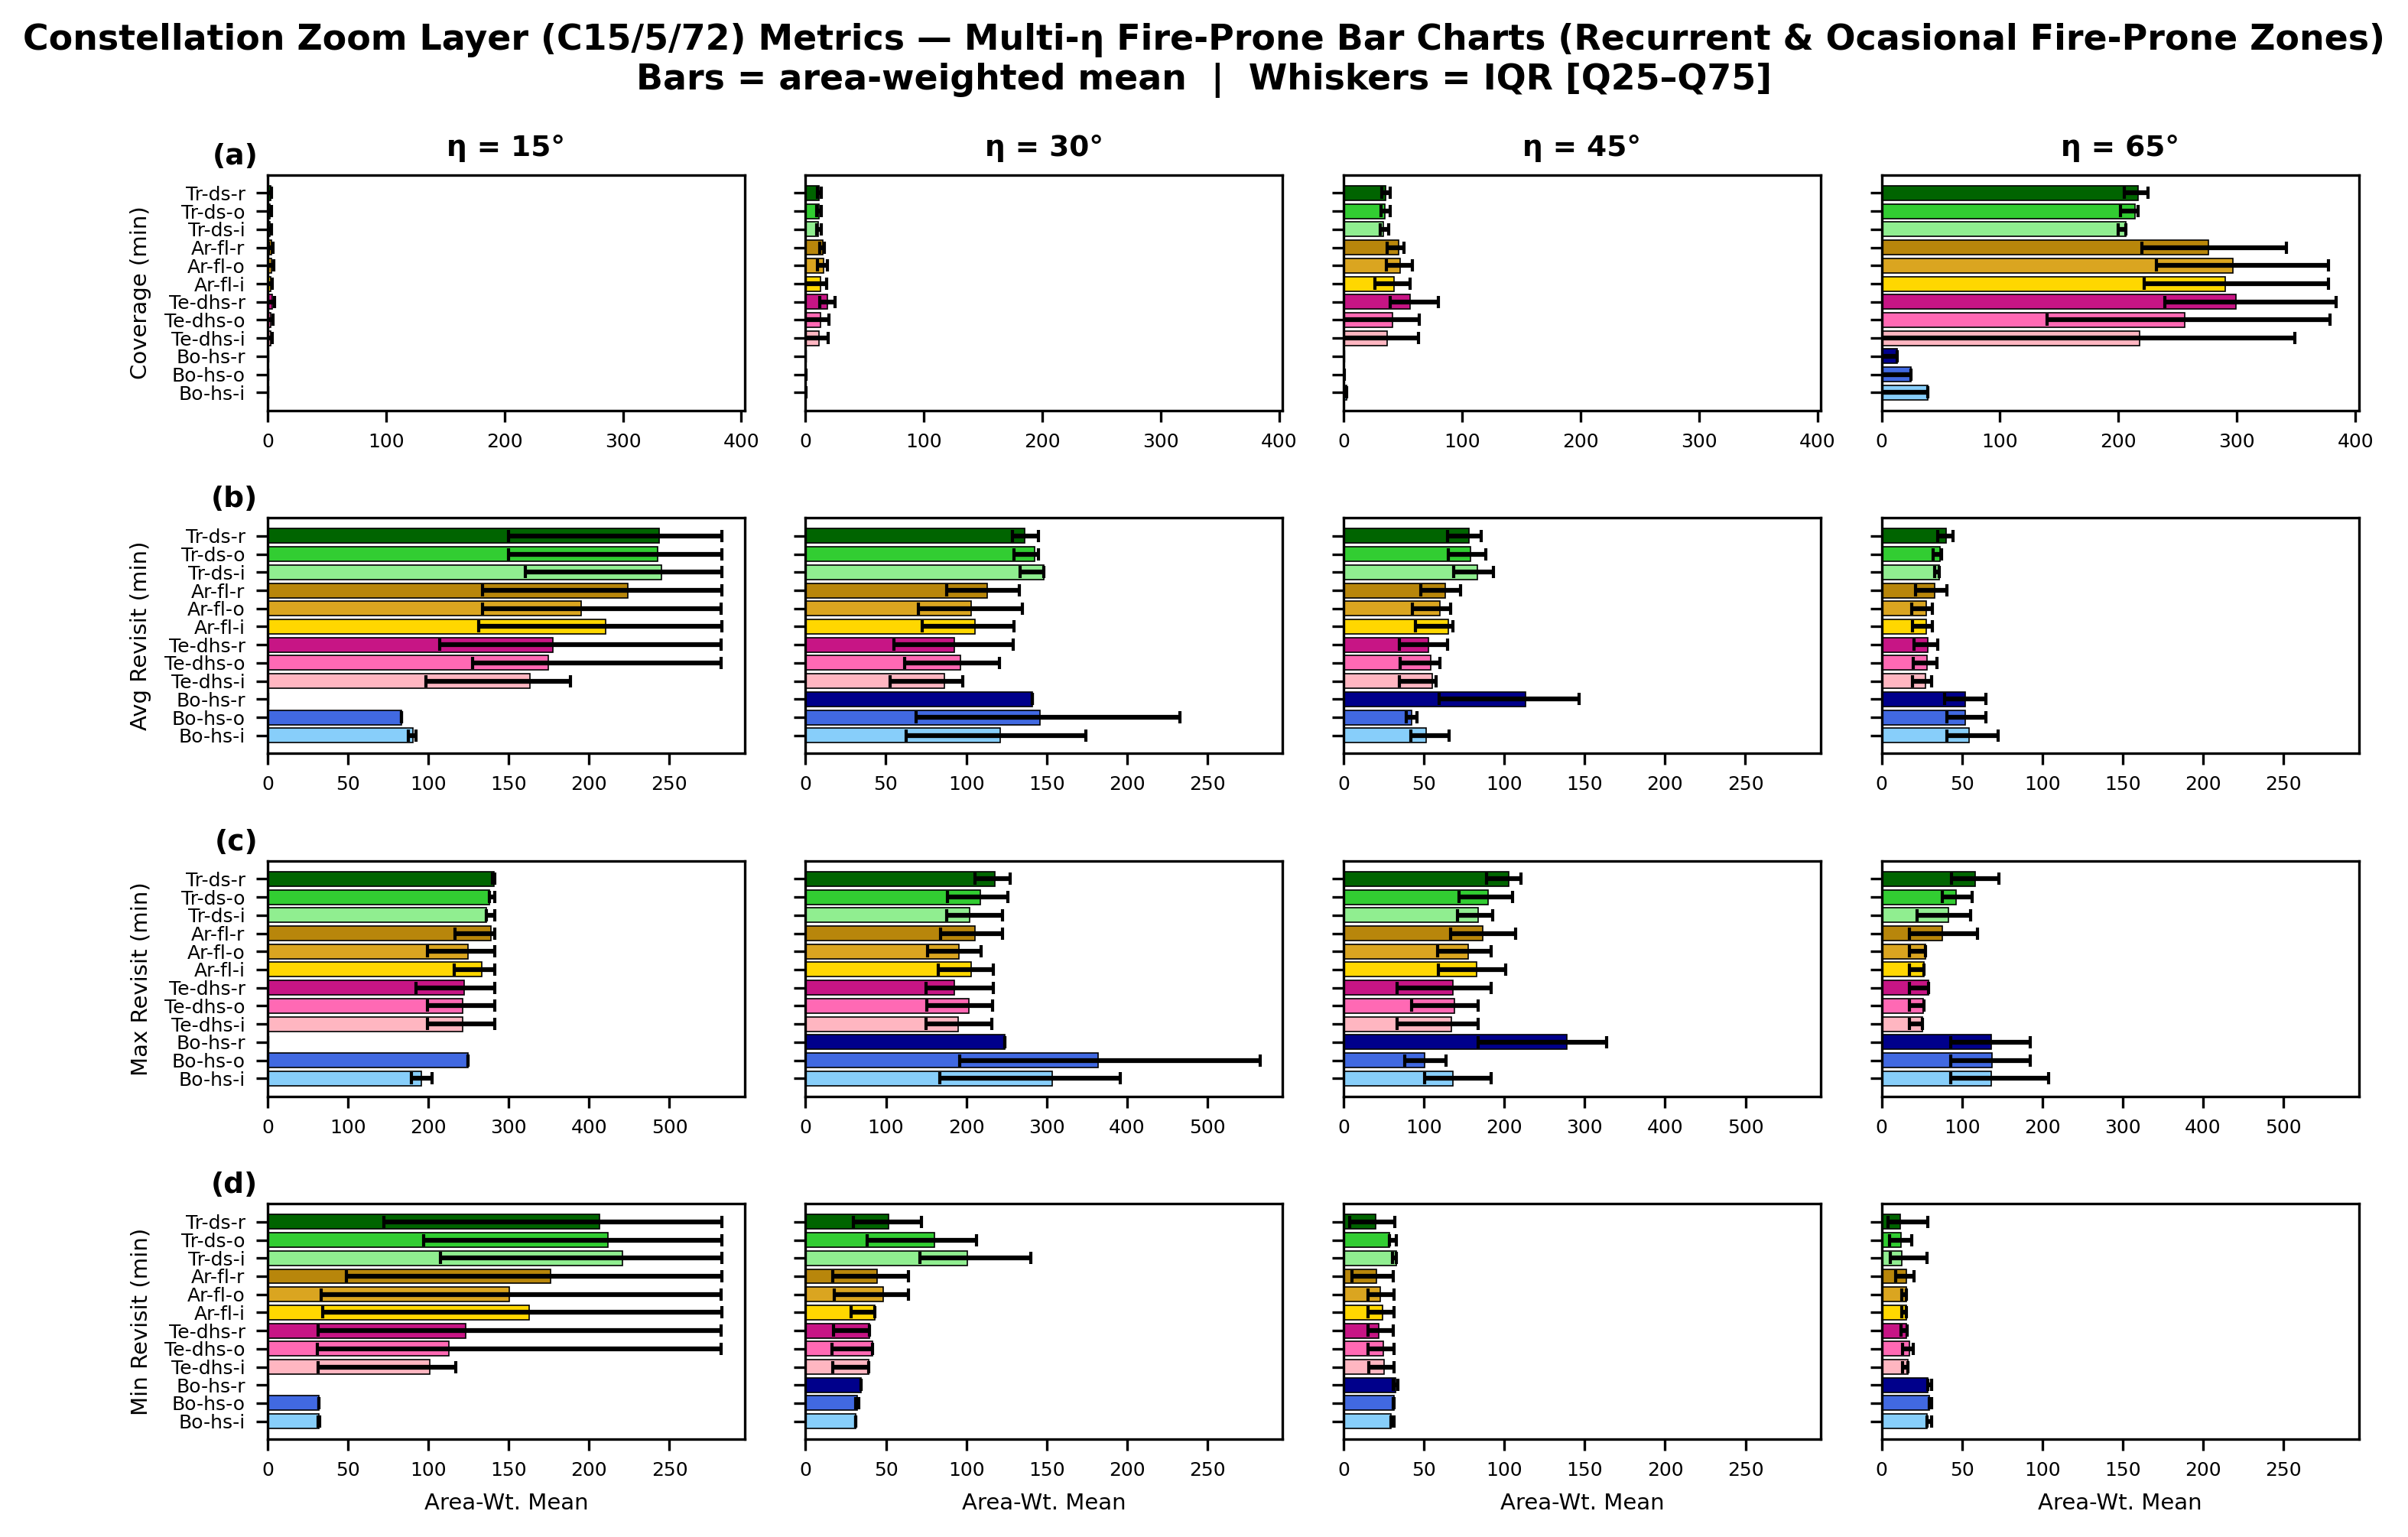
\includegraphics[width=0.85\linewidth,keepaspectratio]{images/c_zoom_metrics_FPR_coverage_statistics_landscape_normalized.png}
    \caption{\footnotesize{Fire-prone region temporal-coverage statistics (normalised) for $\mathcal{C}_{\text{Zoom}}$ across the four $\eta$ configurations ($65^{\circ}$, $45^{\circ}$, $30^{\circ}$, $15^{\circ}$) and the three FPR recurrence groups (recurrent, occasional, infrequent).  Each bar reports the mean $T_{\text{cov}}$ over the masked grid cells; error bars indicate the interquartile range.}}
    \label{fig:c_zoom_metrics_FPR_coverage_statistics}
\end{figure}

\begin{figure}[H]
    \centering
    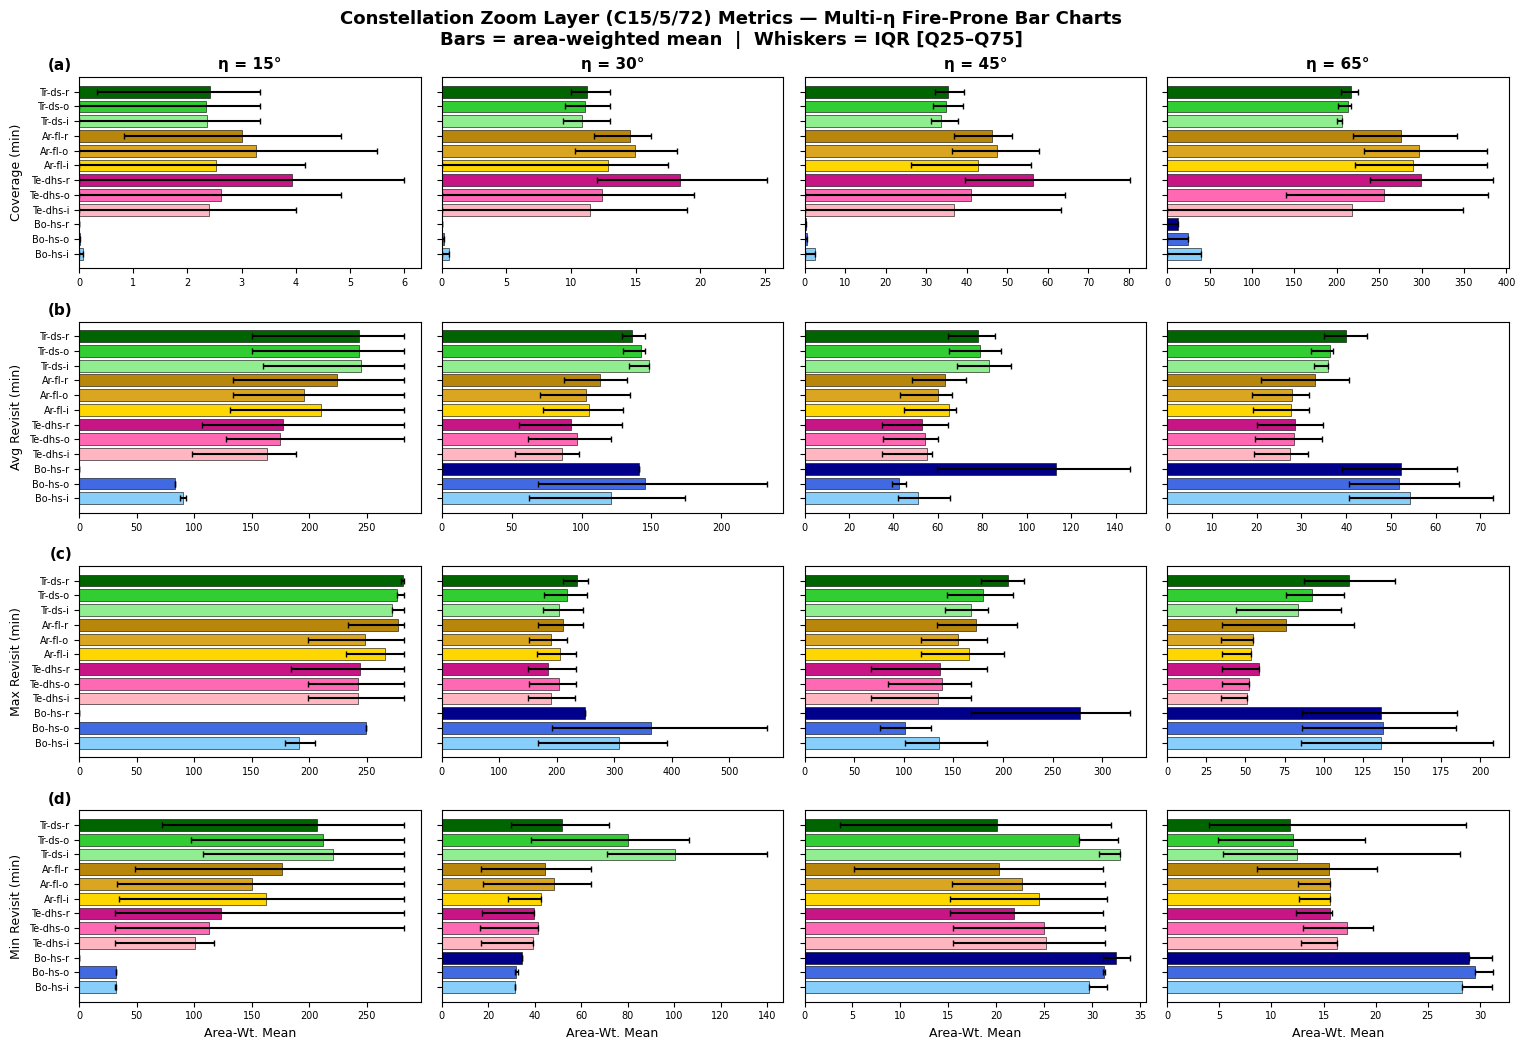
\includegraphics[width=0.85\linewidth,keepaspectratio]{images/c_zoom_metrics_FPR_coverage_statistics_landscape.png}
    \caption{\footnotesize{Fire-prone region temporal-coverage statistics (non-normalised) for $\mathcal{C}_{\text{Zoom}}$ across the four $\eta$ configurations and three FPR recurrence groups.  Absolute $T_{\text{cov}}$ values are shown without per-group normalisation. a) Coverage, b) Average revisit time, c) Max revisit time, d) Min Revisit time}}
    \label{fig:c_zoom_metrics_FPR_coverage_statistics_not_norm}
\end{figure}

\begin{figure}[H]
    \centering
    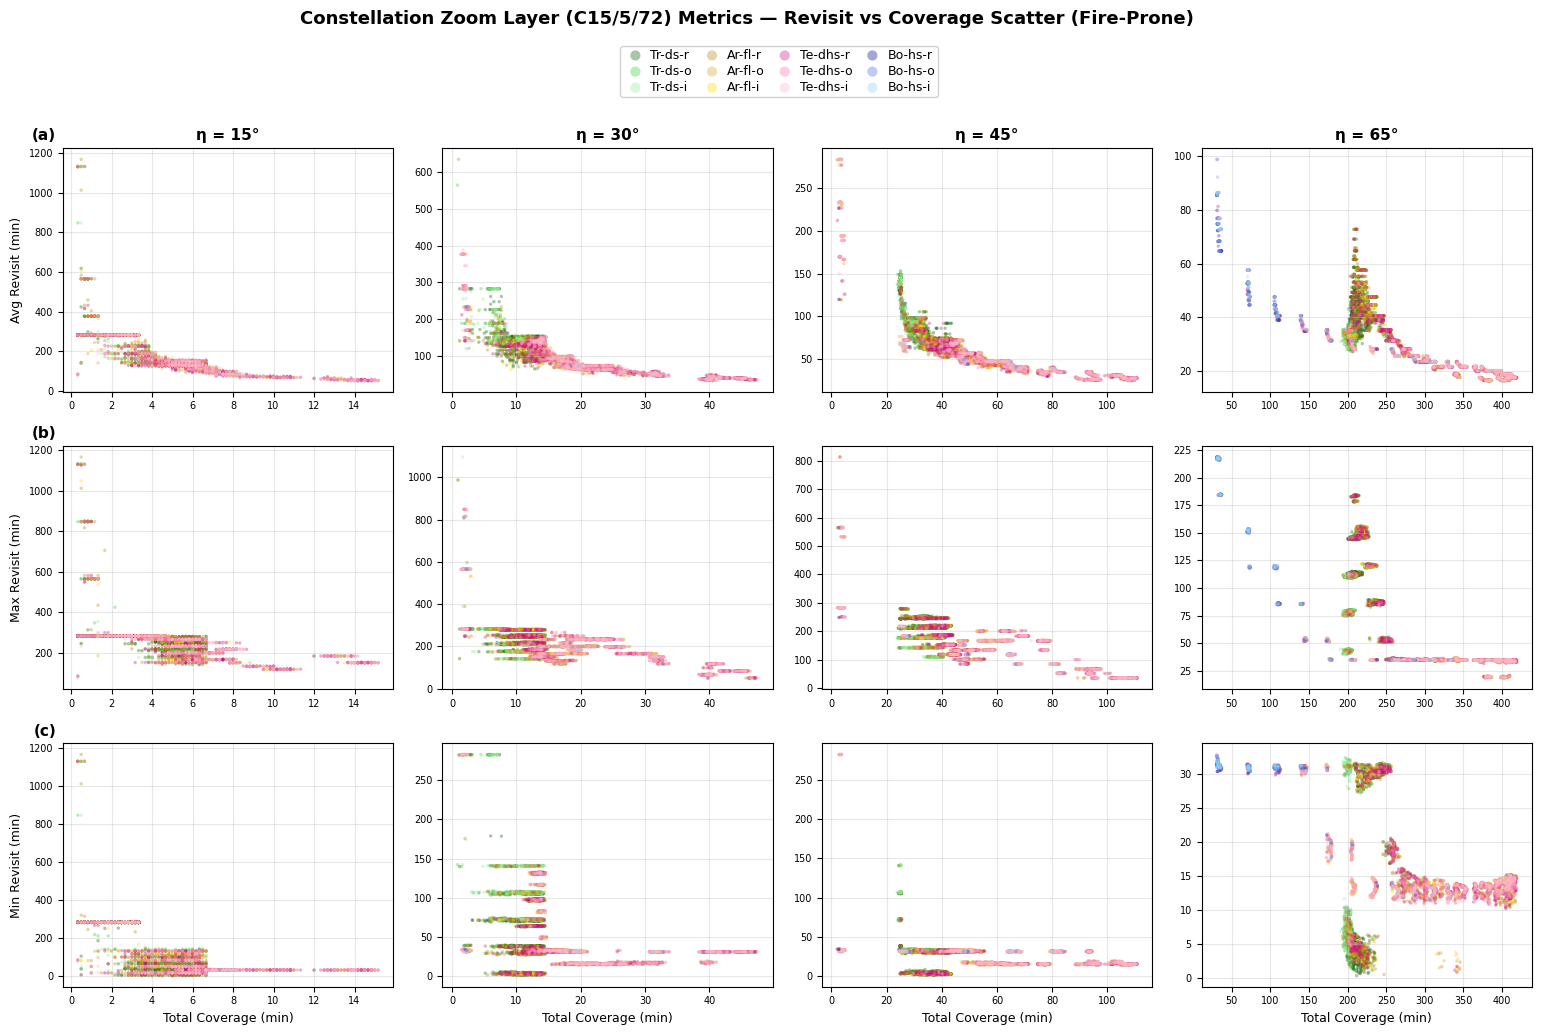
\includegraphics[width=0.85\linewidth,keepaspectratio]{images/c_zoom_metrics_revisitVScoverage_landscape.png}
    \caption{\footnotesize{Revisit time ($\Delta t_{\text{avg}}$) versus temporal coverage ($T_{\text{cov}}$) trade-off for $\mathcal{C}_{\text{Zoom}}$ across FPR recurrence groups and $\eta$ configurations.  Each marker represents one group--$\eta$ combination; wider off-nadir acceptance shifts all groups toward higher coverage and shorter revisit.}}
    \label{fig:c_zoom_metrics_revisitVScoverage}
\end{figure}

\begin{figure}[H]
    \centering
    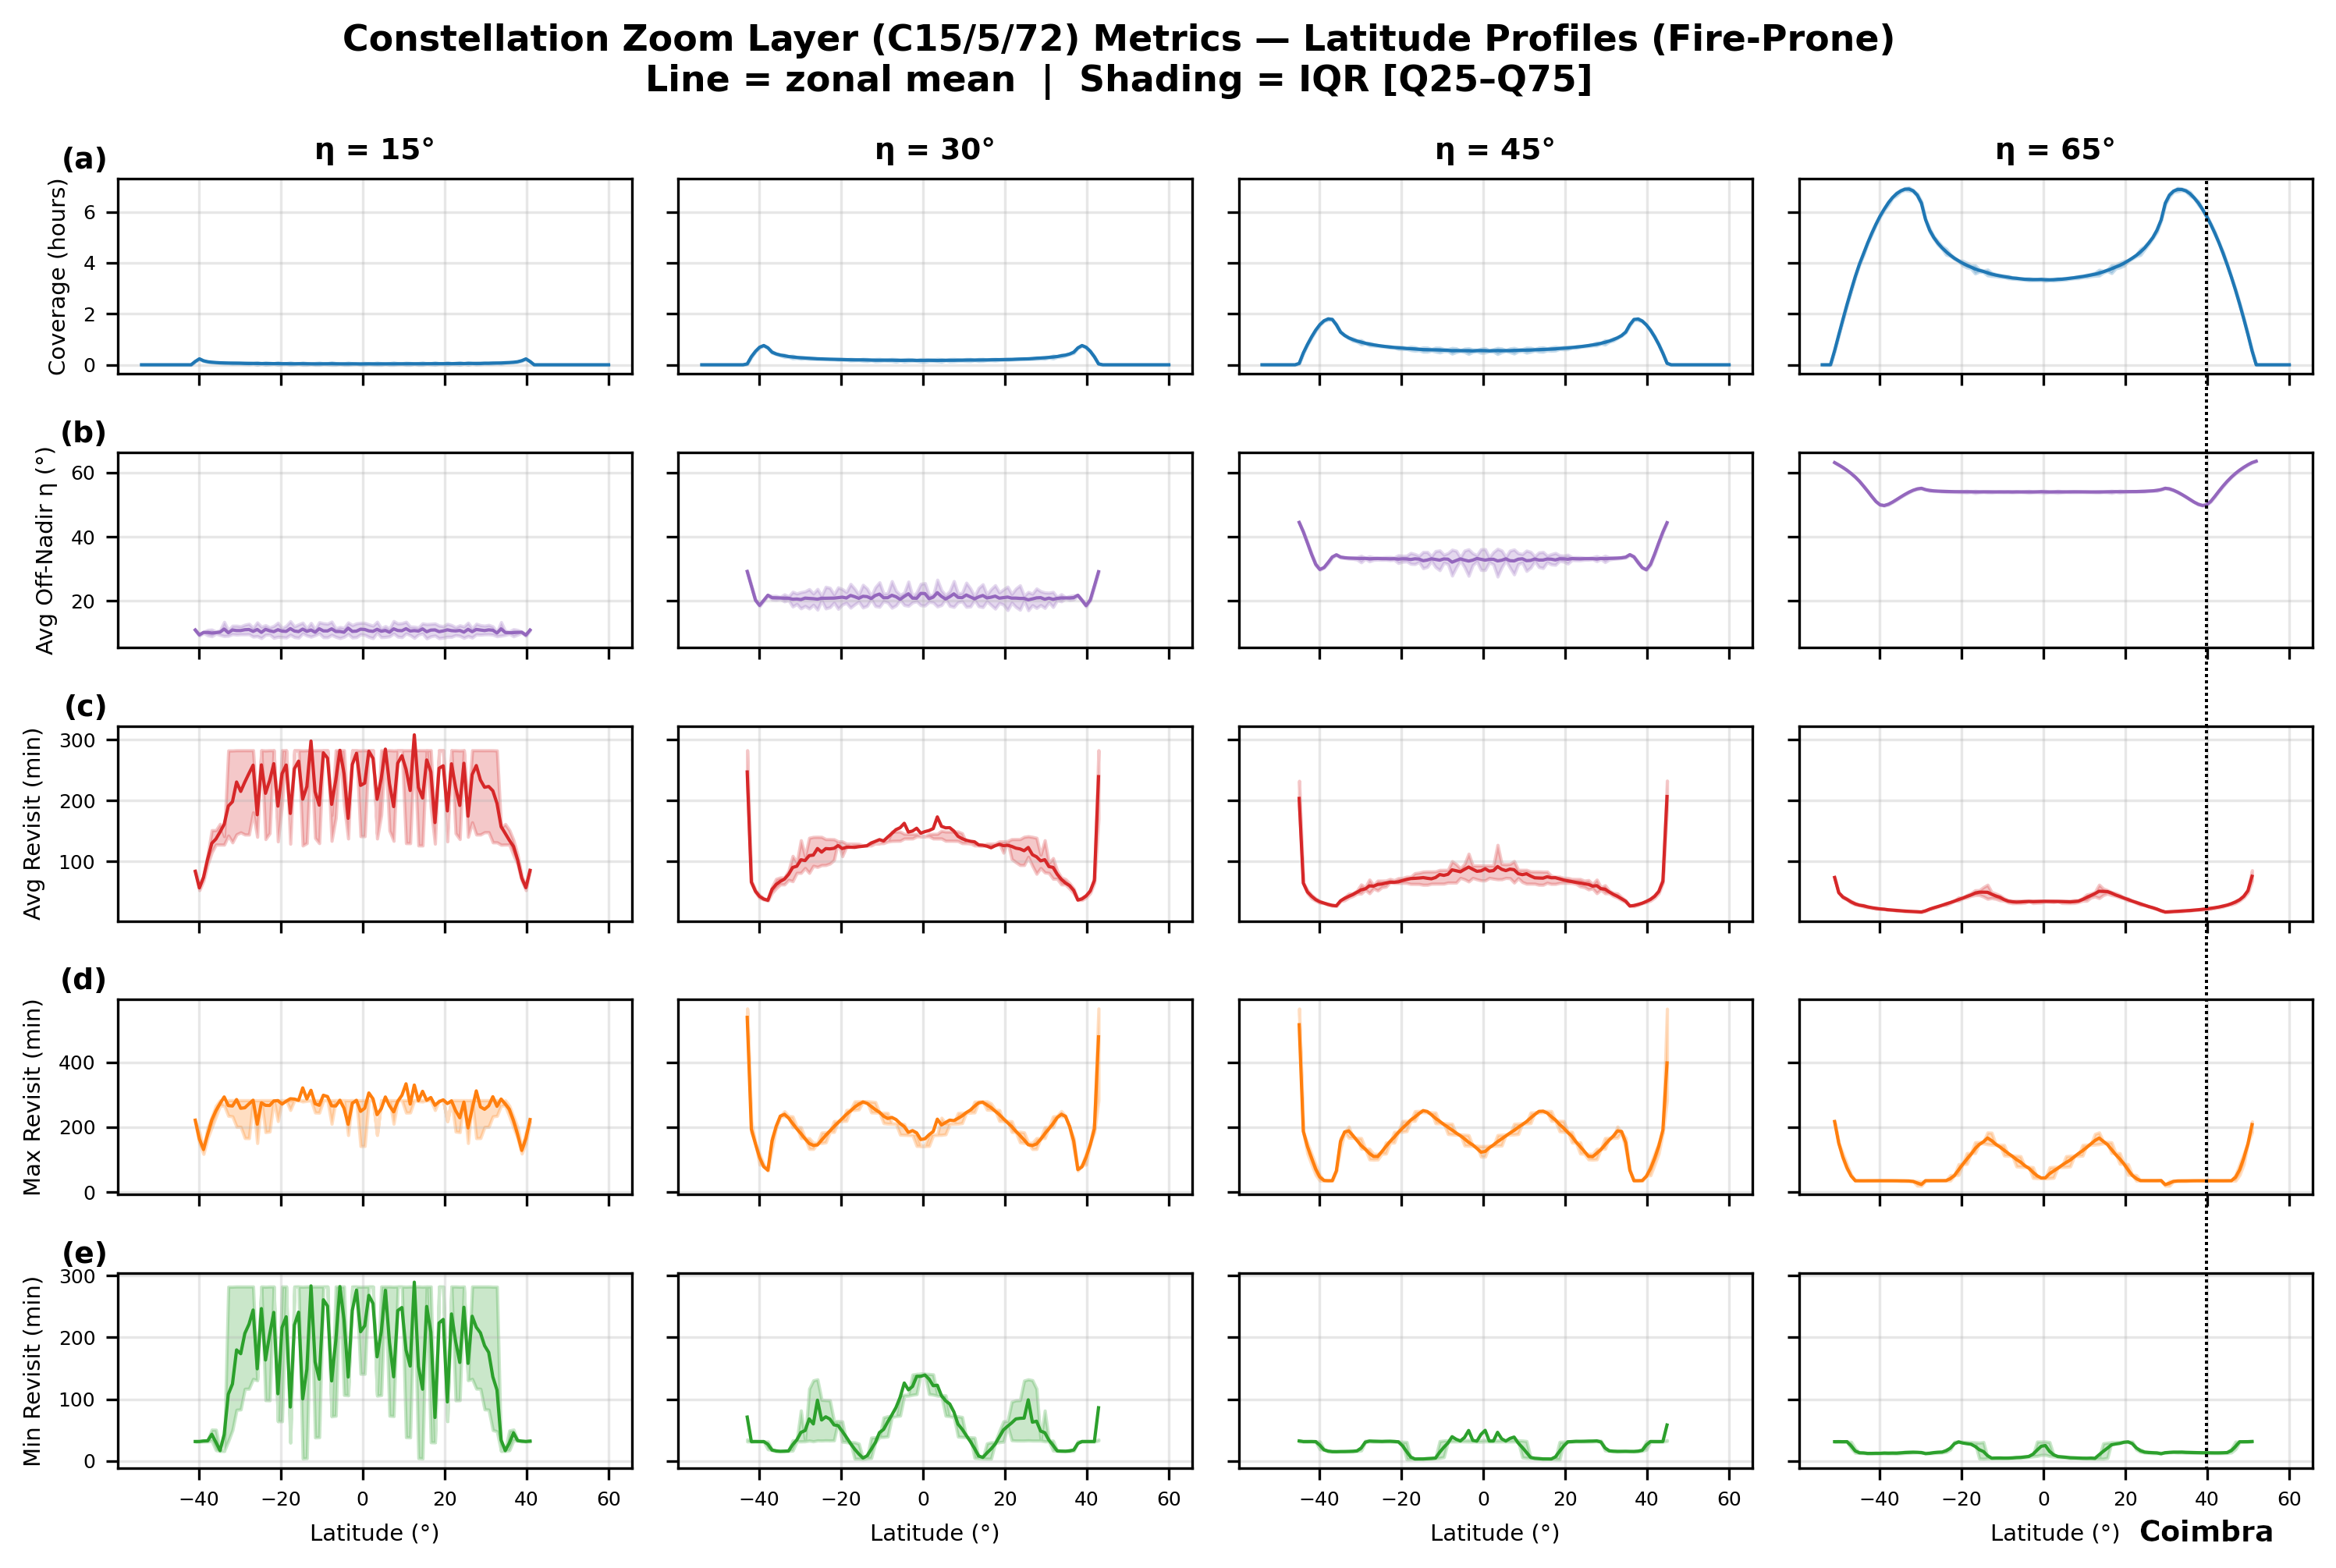
\includegraphics[width=0.85\linewidth,keepaspectratio]{images/c_zoom_metrics_latitude_profile_landscape_normalized.png}
    \caption{\footnotesize{Latitude-dependent temporal-coverage and average-revisit profile (normalised) for $\mathcal{C}_{\text{Zoom}}$ ($\eta = 65^{\circ}$).  Vertical values at $\phi \approx 40^{\circ}$\,N marks the Coimbra core-domain latitude, which falls within the optimal average off-nadir observation angle --- minimum means satellite passes closest to ground nadir axes --- and coverage band. The revisit performance for Portugal is extract from this plot. a) Coverage, b) Average Off-Nadir, c)Average revisit time, d) Max revisit time, e) Min Revisit time}}
    \label{fig:c_zoom_metrics_latitude_profile}
\end{figure}

\begin{figure}[H]
    \centering
    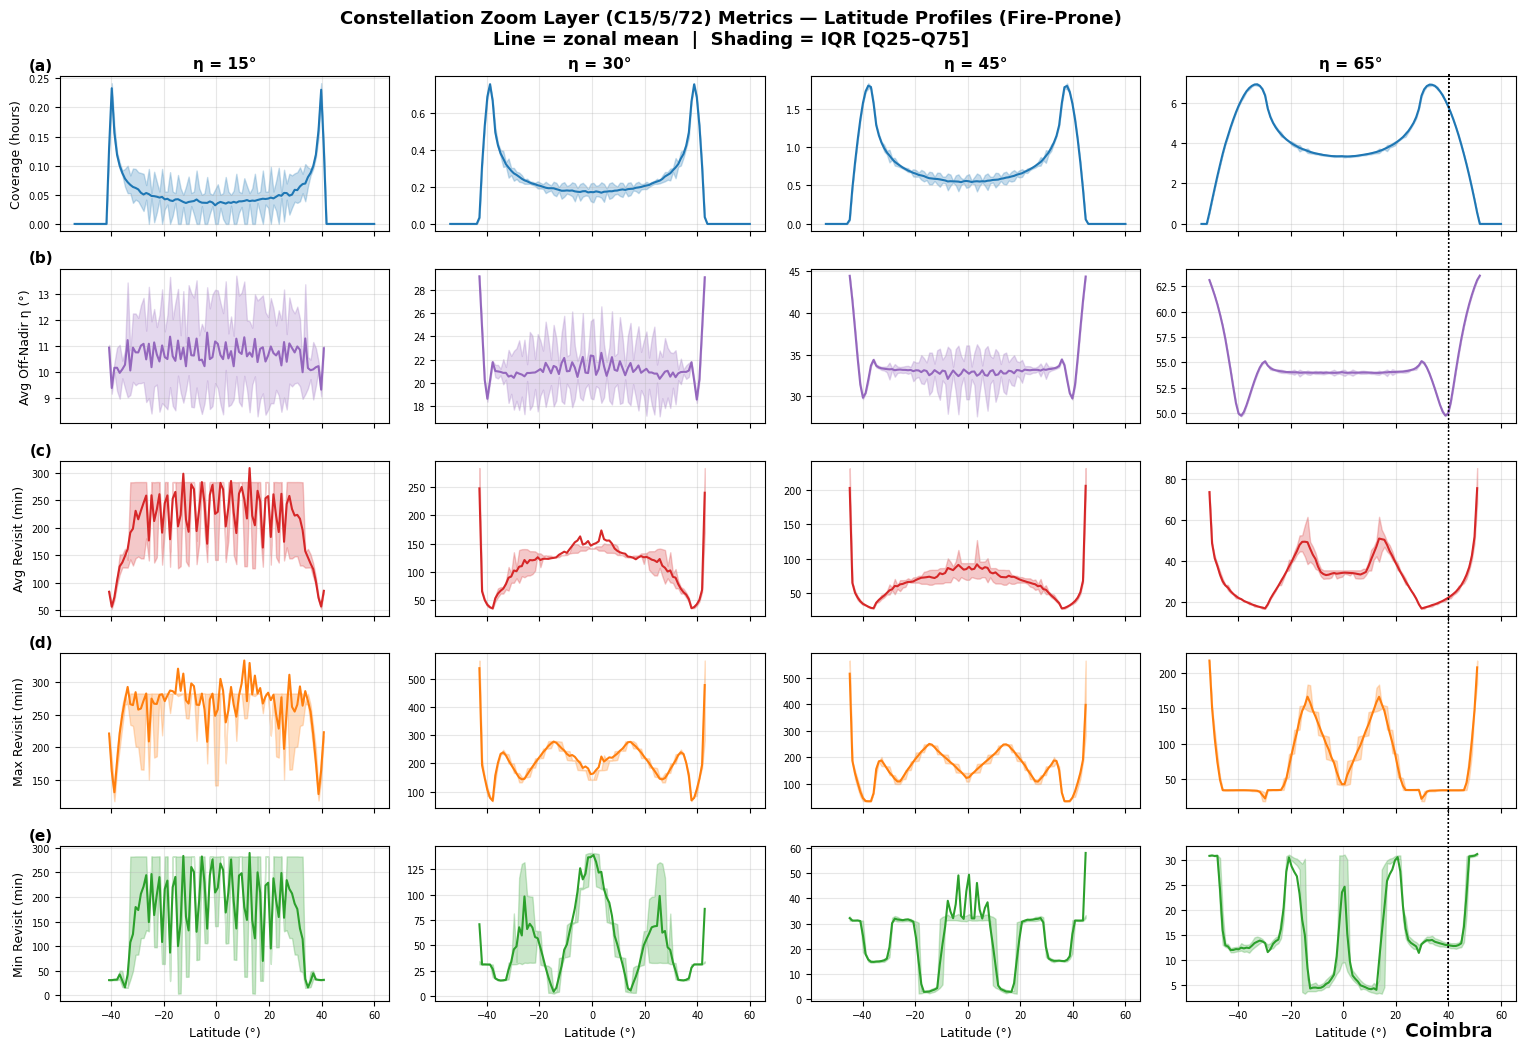
\includegraphics[width=0.85\linewidth,keepaspectratio]{images/c_zoom_metrics_latitude_profile_landscape_not_normalized.png}
    \caption{\footnotesize{Latitude-dependent temporal-coverage and average-revisit profile (non-normalised) for $\mathcal{C}_{\text{Zoom}}$ ($\eta = 65^{\circ}$).Vertical values at $\phi \approx 40^{\circ}$\,N marks the Coimbra core-domain latitude, which falls within the optimal average off-nadir observation angle --- minimum means satellite passes closest to ground nadir axes --- and coverage band. The revisit performance for Portugal is extract from this plot.  Unlike the normalised variant (Fig.~\ref{fig:c_zoom_metrics_latitude_profile}), absolute metric values are plotted on the vertical axes. a) Coverage, b) Average revisit time, c) Max revisit time, d) Min Revisit time.}}
    \label{fig:c_zoom_metrics_latitude_profile_not_norm}
\end{figure}

\end{landscape}
%===================================================
\chapter{Gravitational Perturbations and the Geopotential Model}
\label{app:geopotential}
%===================================================

The Keplerian elements $\vec{A}_k$ (Eq.~\ref{eq:orbital_state_vector}) describe two-body motion under the idealised potential $U_0 = \mu/r$, which assumes a perfectly spherical, homogeneous Earth. In practice, Earth's  rotation produces an equatorial bulge of approximately 21\,km relative to the polar radius, making the geoid an oblate spheroid, as seen in Fig. \ref{fig:earth_oblatenes}. As a consequence, the gravitational potential becomes a function of both geocentric latitude $\varphi_{Gc}$ and longitude $\lambda$, and the realist acceleration acting on satellite $S_k$ deviates from the trajetory prediction from the Keplerian model. This appendix establishes the analytical gravitational potential model \cite{valladoFundamentalsAstrodynamicsApplications2001}, which serves as the foundation for defining orbital perturbation effects exploited by orbit types such as Sun-Synchronous Orbit (SSO, Appendix~\ref{app:sso_orbit}) and Repeating Ground Track Orbit (RGTO). The secular perturbation rates derived from this model---specifically the $J_2$-driven drift rates $\dot{\Omega}$, $\dot{\omega}$, and $\dot{M}$---are the key results used in the main text (Sec.~\ref{sec:perturbed_orbital_elements}) to establish the RGTO resonance condition.

\begin{figure}[H]
    \centering
    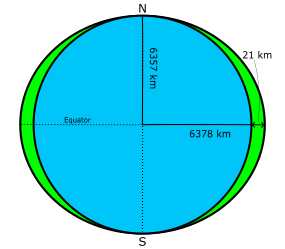
\includegraphics[width=0.4\linewidth]{images/oblateearth.png}
    \caption{\footnotesize{Exaggerated depiction of Earth's oblate shape. The equatorial radius exceeds the polar radius by approximately 21\,km, breaking the spherical symmetry of the gravitational potential $U_0 = \mu/r$. \cite{J2Perturbation}}}
    \label{fig:earth_oblatenes}
\end{figure}

The gravitational potential exterior to the Earth is modelled by an infinite series of spherical harmonics, each term representing a deviation from the uniform spherical case \cite{valladoFundamentalsAstrodynamicsApplications2001}:
\begin{equation}
    U(r, \varphi_{Gc}, \lambda) \;=\; \frac{\mu}{r}
    \left[
        1 + \sum_{L=2}^{\infty} \sum_{M=0}^{L}
        \left( \frac{R_{\oplus}}{r} \right)^{\!L}
        P_{LM}(\sin \varphi_{Gc})\,
        \bigl(
            C_{LM} \cos M\lambda + S_{LM} \sin M\lambda
        \bigr)
    \right],
    \label{eq:geopotential}
\end{equation}
where $r$ is the geocentric distance of $S_k$, $R_{\oplus}$ is Earth's reference equatorial radius, $P_{LM}$ are the associated Legendre polynomials of degree $L$ and order $M$, and $C_{LM}$, $S_{LM}$ are the normalised harmonic coefficients determined empirically from satellite tracking and gravimetry missions. The index pair $(L, M)$ classifies each term by the spatial structure it encodes:
\begin{itemize}
    \item \textbf{Zonal} ($M = 0$): axially symmetric, latitude-dependent only; encode Earth's flattening ($J_2$, $J_3$, \ldots).
    \item \textbf{Sectoral} ($L = M$): longitude-dependent, symmetric about the equatorial plane.
    \item \textbf{Tesseral} ($L \neq M$,\; $M \neq 0$): mixed latitude--longitude variations, encoding the ``lumpy'' mass distribution.
\end{itemize}

\begin{figure}[H]
    \centering
    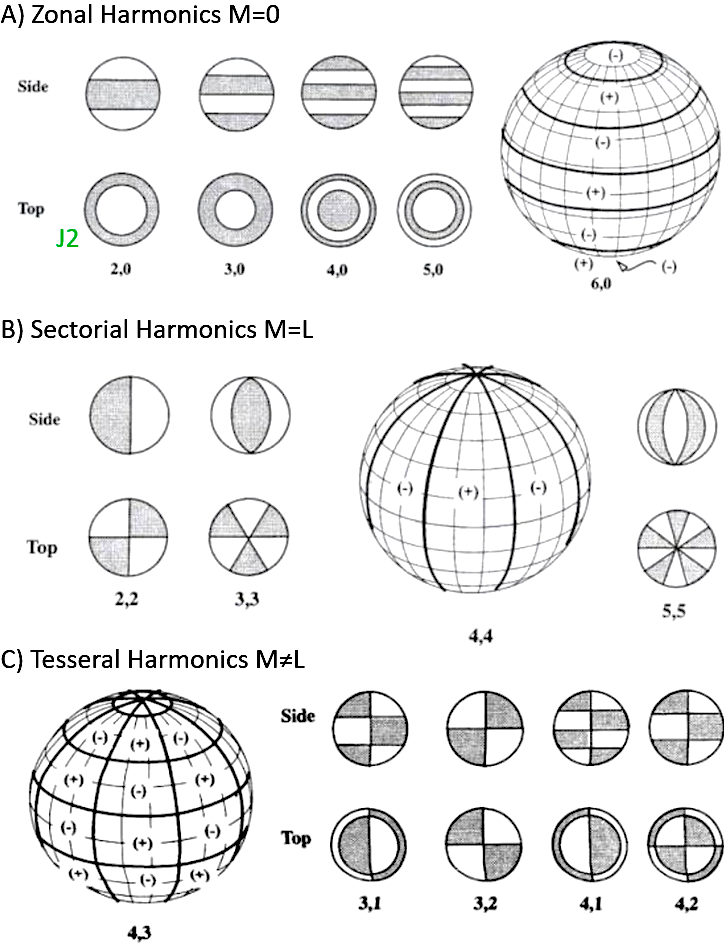
\includegraphics[width=0.5\linewidth]{images/geopotencial_harmonics.png}
    \caption{\footnotesize{Zonal ($M=0$), sectoral ($L=M$), and tesseral ($L \neq M$, $M\neq 0$) spherical harmonic modes of the geopotential. Increasing degree $L$ and order $M$ subdivide the sphere into progressively finer latitude and longitude bands. \cite{lgeorge2Chapter10Orbital, valladoFundamentalsAstrodynamicsApplications2001}}}
    \label{fig:geopotential_harmonics_zonal_sectorial_tectral}
\end{figure}

%===================================================
\section{The Dominant \texorpdfstring{$J_2$}{J2} Perturbation}
\label{sec:j2pert}
%===================================================

Among all harmonic terms in Eq.~\ref{eq:geopotential}, the second zonal coefficient $J_2 \equiv -C_{20} \approx 1.08263 \times 10^{-3}$ is by far the largest, exceeding the next significant coefficient by approximately three orders of magnitude (Table~\ref{tab:harmonic_coefficients}). It quantifies the oblateness that is already visible in Fig.~\ref{fig:earth_oblatenes}. Using only this term, Eq.~\ref{eq:geopotential} reduces to the $J_2$-perturbed potential:
\begin{equation}
    U_{J_2}(r,\theta) \;=\; \frac{\mu}{r}\left[
        1 - J_2 \left(\frac{R_{\oplus}}{r}\right)^{\!2} P_2(\cos\theta)
    \right],
    \label{eq:potential_j2}
\end{equation}
where $P_2(\cos\theta) = \tfrac{1}{2}(3\cos^2\theta - 1)$ is the second Legendre polynomial and $\theta$ is the colatitude.

\begin{table}[H]
\centering
\caption{\footnotesize{Representative values of the dominant geopotential harmonic coefficients. $J_n \equiv -C_{n0}$ are the zonal coefficients; $C_{LM}$, $S_{LM}$ are tesseral/sectoral coefficients. $J_2$ exceeds all others by approximately three orders of magnitude. \cite{valladoFundamentalsAstrodynamicsApplications2001}}}
\label{tab:harmonic_coefficients}
\begin{tabular}{lll}
\toprule
Coefficient & Value & Physical description \\
\midrule
$J_2$            & $\phantom{-}1.08263 \times 10^{-3}$  & Dominant equatorial bulge (oblateness)     \\
$J_3$            & $-2.532 \times 10^{-6}$               & Pear-shaped north--south asymmetry         \\
$J_4$            & $-1.620 \times 10^{-6}$               & Higher-order zonal correction              \\
$J_5$            & $-2.277 \times 10^{-7}$               & Higher-order zonal variation               \\
$J_6$            & $\phantom{-}5.406 \times 10^{-7}$     & Further refinement of Earth's shape        \\
$C_{22}$         & $\phantom{-}1.574 \times 10^{-6}$     & Sectoral: equatorial ellipticity           \\
$S_{22}$         & $-1.867 \times 10^{-6}$               & Sectoral variation                         \\
$C_{21},\,S_{21}$& ${\sim}1 \times 10^{-6}$              & Tesseral terms (low degree/order)          \\
\bottomrule
\end{tabular}
\end{table}

\begin{figure}[H]
    \centering
    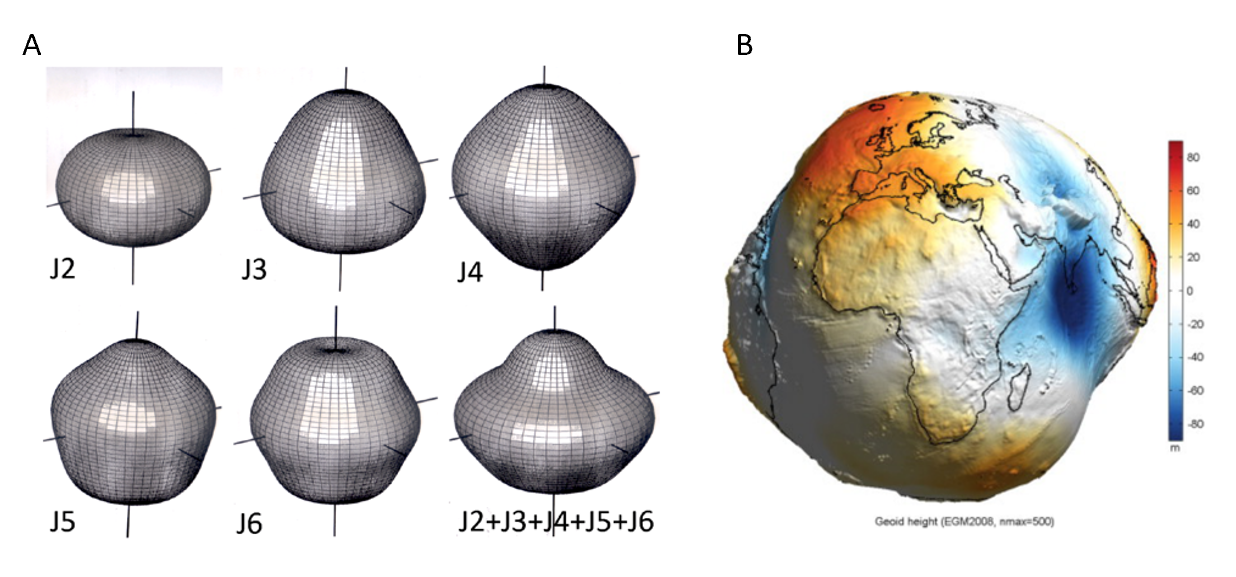
\includegraphics[width=0.5\linewidth]{images/geoid_gravitational_Example_hamoci_comparation.png}
    \caption{\footnotesize{Left: spatial patterns for selected harmonic degrees. Right: geoid height relative to the EGM2008 gravitational field model \cite{barnesEarthGravitationalModel2015}, produced using over 2000 harmonic coefficients. The $J_2$ contribution dominates the large-scale structure; higher-order terms refine local variations. \cite{lgeorge2Chapter10Orbital}}}
    \label{fig:geoid_Graviational_example_harmonics_comparation}
\end{figure}

%% ======================================================================
%% APPENDIX — Sun-Synchronous Orbit Analysis and RGTO Comparison
%% ======================================================================
\chapter{Comparison between Sun-Synchronous Orbit and Repeating Ground Track Orbit}
\label{app:sso_orbit}

This appendix develops the astrodynamic theory of the Sun-Synchronous Orbit (SSO) and presents a quantitative comparison between the SSO and the Repeating Ground Track Orbit (RGTO) seed adopted in the main text.  The SSO is included as a commercially motivated comparison baseline: it is the predominant LEO orbit class for Earth observation, and its widespread availability via rideshare launches makes it the natural benchmark against which the mission-specific RGTO design is evaluated.

%% ------------------------------------------------------------------
\section{Sun-Synchronous Orbit (SSO)}
\label{72-SSO_intro}
%% ------------------------------------------------------------------

A \textbf{Sun-Synchronous Orbit} (SSO) is a near-polar, retrograde orbit ($i > 90^{\circ}$) whose orbital plane precesses eastward at exactly the rate at which the Earth revolves around the Sun, therefore maintaining a constant angle between the orbital plane and the Earth--Sun direction throughout the year.  This property guarantees repeatable solar illumination conditions at each latitude crossing, making SSOs the predominant choice for optical and multispectral Earth-observation missions. This section defines the equations used to model SSO to create a comparison with the RGTO case. The equations are based on Vallado's book \cite{valladoFundamentalsAstrodynamicsApplications2001}.

\subsection{Sun-Synchronous Condition}
\label{sec:sso_condition}

The SSO condition requires that the secular nodal regression rate $\dot{\Omega}$ (Eq.~\eqref{eq:dot_Omega}) matches the mean angular velocity of the Earth's orbital motion around the Sun:
\begin{equation}
    \dot{\Omega}_{\mathrm{SSO}} = \frac{2\pi}{T_{\odot}} \approx 1.991 \times 10^{-7}\;\mathrm{rad\,s^{-1}},
    \label{eq:sso_omega_dot}
\end{equation}
where $T_{\odot} = 365.2421897\;\mathrm{d}$ is the mean tropical year.  Substituting Eq.~\eqref{eq:dot_Omega} into this condition yields the fundamental SSO design equation relating $a$, $e$, and $i$:
\begin{equation}
    -\frac{3}{2}\,J_2 \left(\frac{R_{\oplus}}{p}\right)^{\!2} \sqrt{\frac{\mu_{\oplus}}{a^3}}\,\cos i \;=\; \dot{\Omega}_{\mathrm{SSO}},
    \label{eq:sso_fundamental}
\end{equation}
where $p = a(1 - e^2)$ is the semi-latus rectum.  Because the required nodal precession is eastward ($\dot{\Omega} > 0$) and $\dot{\Omega} \propto -\cos i$, the cosine of the inclination must be negative, constraining $i > 90^{\circ}$ (retrograde orbit).

\subsection{Inclination from Semi-Major Axis}
\label{sec:sso_inc_from_a}

For a given semi-major axis $a$ and eccentricity $e$, solving Eq.~\eqref{eq:sso_fundamental} for inclination yields~\cite[Eq.~11-15]{valladoFundamentalsAstrodynamicsApplications2001}:
\begin{equation}
    i_{\mathrm{SSO}} = \arccos\!\left(-\frac{2\,\dot{\Omega}_{\mathrm{SSO}}\,a^{7/2}\,(1 - e^2)^2}{3\,J_2\,R_{\oplus}^2\,\sqrt{\mu_{\oplus}}}\right).
    \label{eq:sso_inclination}
\end{equation}
This expression is the primary design equation used to define a SSO: given $a$ and $e$, the sun-synchronous inclination is uniquely determined.

\subsection{Semi-Major Axis from Inclination}
\label{sec:sso_a_from_inc}

Conversely, if the inclination is prescribed, the required semi-major axis is obtained by rearranging Eq.~\eqref{eq:sso_fundamental}~\cite[Eq.~11-14]{valladoFundamentalsAstrodynamicsApplications2001}:
\begin{equation}
    a_{\mathrm{SSO}} = \left(\frac{-3\,J_2\,R_{\oplus}^2\,\sqrt{\mu_{\oplus}}\,\cos i}{2\,\dot{\Omega}_{\mathrm{SSO}}\,(1 - e^2)^2}\right)^{\!2/7}.
    \label{eq:sso_sma}
\end{equation}

\subsection{Eccentricity from Semi-Major Axis and Inclination}
\label{sec:sso_ecc}

When both $a$ and $i$ are fixed, the eccentricity compatible with the sun-synchronous condition follows from~\cite[Eq.~11-16]{valladoFundamentalsAstrodynamicsApplications2001}:
\begin{equation}
    e_{\mathrm{SSO}} = \sqrt{1 - \sqrt{\frac{-3\,J_2\,R_{\oplus}^2\,\sqrt{\mu_{\oplus}}\,\cos i}{2\,a^{7/2}\,\dot{\Omega}_{\mathrm{SSO}}}}}\,.
    \label{eq:sso_ecc}
\end{equation}
Equations~\eqref{eq:sso_inclination}--\eqref{eq:sso_ecc} form a closed system: specifying any two of $(a,\,e,\,i)$ uniquely determines the third under the SSO constraint.

\subsection{RAAN and Local Time of the Ascending Node (LTAN)}
\label{sec:sso_ltan}

A defining operational parameter of any SSO is the \textbf{Local Time of the Ascending Node} (LTAN), which specifies the local solar time at which the satellite crosses the equator northbound.  Given a reference epoch $t_0$ and the Sun's apparent right ascension $\alpha_{\odot}(t_0)$ at that epoch, the RAAN required to achieve a desired LTAN is:
\begin{equation}
    \Omega_{\mathrm{SSO}} = \alpha_{\odot}(t_0) + \bigl(\mathrm{LTAN}_{\mathrm{h}} - 12\bigr) \times 15^{\circ},
    \label{eq:sso_raan_ltan}
\end{equation}
where $\mathrm{LTAN}_{\mathrm{h}}$ is the LTAN expressed in hours.  Common choices include $\mathrm{LTAN} = 06\!:\!00$ (dawn--dusk, minimal shadow) and $\mathrm{LTAN} = 10\!:\!30$ (morning descending node with favourable illumination for optical imaging).

\subsection{SSO Orbital Element Vector}
\label{sec:sso_element_vector}

Analogously to the RGTO element vector (Eq.~\eqref{eq:rgto_element_vector}), the SSO orbit of satellite $S_k$ is fully specified by:
\begin{equation}
    \vec{\mathbf{A}}^{\,\mathrm{SSO}}{}_{k} = \bigl[a,\; e,\; i_{\mathrm{SSO}},\; \omega,\; \Omega,\; \nu,\; t_0\bigr]^{T},
    \label{eq:sso_element_vector}
\end{equation}
where $i_{\mathrm{SSO}}$ is obtained from Eq.~\eqref{eq:sso_inclination}.  Unlike the RGTO, where the period ratio $\tau$ replaces $a$ as the independent design parameter, in the SSO the semi-major axis $a$ remains the primary free parameter because the inclination is uniquely determined by the sun-synchronous condition for a given $(a, e)$ pair.

%% ------------------------------------------------------------------
\section{SSO Seed Orbit Parameters}
\label{sct-SSO_seed}
%% ------------------------------------------------------------------

The SSO seed orbit is selected to represent the most operationally accessible orbit class for LEO Earth observation.  The majority of small-satellite launches to LEO utilise rideshare services on reusable launch vehicles, such as SpaceX Falcon~9 Transporter mission, which inject payloads into a common SSO defined by the launch provider's target semi-major axis and epoch.  This shared-ride operation makes the SpaceX rideshare SSO the reference orbit for cost-constrained LEO missions. Therefore, we adopt this orbit as the SSO baseline, ensuring a comparison with the RGTO seed and reflecting a realistic, commercially available alternative.

As explained in Section~\ref{72-SSO_intro}, the SSO seed is completely determined by two independent parameters: the semi-major axis $a$ and the insertion epoch~$t_0$.  Given these, the $J_2$-driven sun-synchronous condition (Eq.~\eqref{eq:sso_inclination}) defines the inclination $i_{\mathrm{SSO}}$ such that the secular nodal regression rate $\dot{\Omega}$ (Eq.~\eqref{eq:dot_Omega}) exactly compensates the apparent motion of the Sun, maintaining a constant orbital-plane orientation with respect to the Earth--Sun line throughout the year.

Using as example the SpaceX Transporter injection parameters ($a = 6904$\,km, $e = 0.0$, epoch 2021-01-24T15:00\,UTC), the SSO conditions  (Sec.~\ref{sec:sso_condition}) yields the SSO seed orbital element vector:
\begin{equation}
    \vec{\mathbf{A}}^{\,\mathrm{SSO}}{}_{0} = \bigl[6904\;\mathrm{km},\; 0.0,\; 97.50^{\circ},\; 0^{\circ},\; 0^{\circ},\; 0^{\circ},\; t_0\bigr]^{T},
    \label{eq:sso_seed_vector}
\end{equation}
where $t_0 = \text{2021-01-24T15:00 UTC}$.  Table~\ref{tab:sso_seed_parameters} summarises the complete set of derived parameters for this seed orbit.

\begin{table}[H]
\centering
\caption{\footnotesize{SSO seed orbit parameters derived from the SpaceX Transporter rideshare injection conditions ($^{\ddagger}$).  The inclination $i_{\mathrm{SSO}}$ is computed from the sun-synchronous condition (Eq.~\eqref{eq:sso_inclination}); all other quantities follow from the standard $J_2$ secular perturbation model.  Common conditions: $e = 0.0$, $\omega = 0^{\circ}$, $\Omega = 0^{\circ}$, $M = 0^{\circ}$.}}
\label{tab:sso_seed_parameters}
\smallskip
\footnotesize
\setlength{\tabcolsep}{4pt}
\begin{tabular}{l r r r r r }
\toprule
Orbit
  & $a$ [km]
  & $h$ [km]
  & $e$
  & $i_{\mathrm{SSO}}$ [$^{\circ}$]
  & $\dot{\Omega}_{\mathrm{SSO}}$ [rad\,s$^{-1}$]
  \\
\midrule
SpaceX Transporter & 6904.00 & 525.86 & 0.0 & 97.50 & $1.991{\times}10^{-7}$ \\
\bottomrule
\end{tabular}
\\[2pt]
{\footnotesize \parbox{0.97\linewidth}{$^{\ddagger}$ Insertion epoch $t_0 = \text{2021-01-24T15:00 UTC}$.  Constants used: $\mu_{\oplus} = 3.986{\times}10^{5}$\,km$^{3}$\,s$^{-2}$, $R_{\oplus} = 6378.10$\,km, $J_2 = 1.08263{\times}10^{-3}$.}}
\end{table}

%% ------------------------------------------------------------------
\section{RGTO vs.\ SSO: Observation-Link Comparison}
\label{sct-rgto_vs_sso}
%% ------------------------------------------------------------------

The resulting SSO altitude of $h \approx 525.9$\,km places this orbit within the same LEO Earth-observation band as the RGTO seed ($h \approx 488.5$\,km, Table~\ref{tab:rgto_parameters_coimbra}), enabling a direct comparison of coverage performance under comparable GSD conditions.  However, the SSO inclination ($i_{SSO} \approx 97.5^{\circ}$) is very different from the RGTO inclination ($i_{RGTO} = 40.2^{\circ}$), which is geometrically aligned to the Coimbra target latitude.  This mismatch is the primary driver of the coverage differences analysed in this section.

A geometrical comparison is done in Fig~\ref{fig:rgtoVSsso_7day_prop_maps}  where propagation of 7 days is done for orbits $\vec{\mathbf{A}}^{\,\mathrm{RGTO}^{\,2}}{}_{0,\,\mathrm{Coimbra}}$ , and $\vec{\mathbf{A}}^{\,\mathrm{SSO}}{}_{0}$. The near-polar SSO crosses the target latitude at a steep angle with limited permanence time, whereas the RGTO ground track aligns with the target latitude, maximising both pass duration and the number of daily revisits. This is a critical factor to increase the sensor's effective FOV.
\begin{figure}[H]
    \centering
    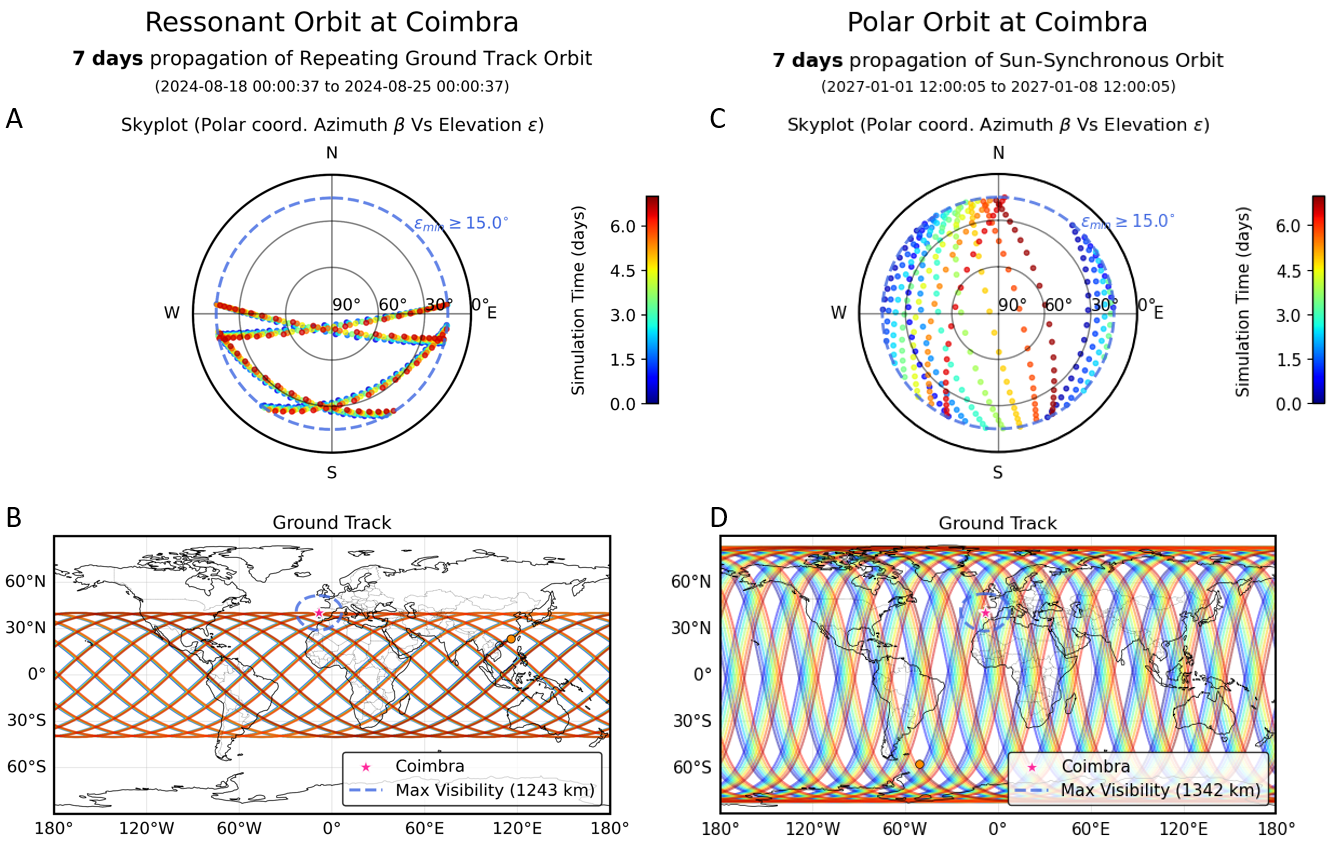
\includegraphics[width=1\linewidth]{images/rgtoVSsso_7days_prop_maps.png}
    \caption{\footnotesize{Plots C and D show the SSO ground track crossing the target latitude at a steep angle (South-North direction) with limited permanence time; on the other hand, plots A and B show the RGTO ground track aligned with the target at Coimbra latitude, maximizing both pass duration and the number of daily revisits. The difference in elevation between the two plots is also evident in the density and geometric distribution of the skyplots. SSO has greater density at low elevations, while RGTO has a more uniform elevation distribution. This has a significant impact on the sensor's effective FOV for achieving observation link access to the ground target.}}
    \label{fig:rgtoVSsso_7day_prop_maps}
\end{figure}


Further details on the necessary sensor trade-off are shown in Figure \ref{fig:rgtoVSsso_7day_prop_old}, which compares the same 7-day propagation RGTO and SSO seeds over Coimbra across three metrics: visibility windows, elevation--distance profile, and off-nadir $\eta$ angle versus Ground Sample Distance (GSD).  The RGTO produces four approximately visible windows with $\eta<60^\circ$ per 24-hour cycle, all exceeding $\varepsilon > 15^{\circ}$ elevation, yielding low off-nadir angles and consequently a GSD well within the mission requirement, totalizing 28 passes over 7 days.  The SSO, governed by its 12-hour repeat cycle, provides only two windows per pass burst at significantly lower elevations, which degrade the observation link geometry and inflate the effective FOV, totalizing 16 passes over 7 days.  
The comparison indicates that approximately 1.75 times as many SSO satellites would be required to match the temporal and spatial coverage delivered by a single RGTO plane. Therefore, the RGTO is preferred for this mission design. 

It is also important to note that SSO orbits are cheaper to reach due to ride-sharing on reusable rockets, and that this orbit is more populated and carries a higher risk of space debris. RGTO can also be achieved with reusable rockets; a trade-off between cost and performance should be made in a future study. For this work, we focus on the best coverage case for the study domain: the RGTO case.

\begin{figure}[H]
    \centering
    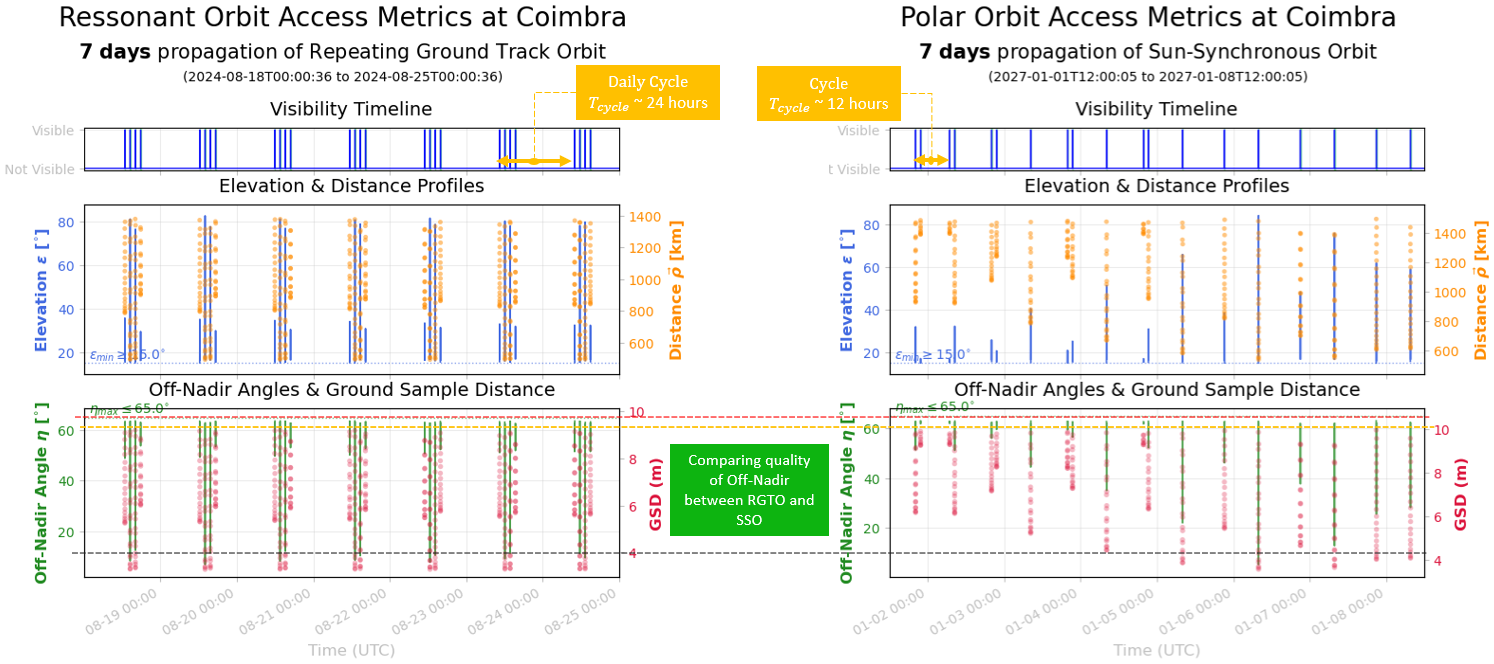
\includegraphics[width=1\linewidth]{images/rgtoVSsso_7days_prop.png}
    \caption{\footnotesize{Observation-link comparison over Coimbra ($\phi_{\text{lat}}=40.2^{\circ}$\,N) for a 7-day propagation.  \textbf{Left column}: RGTO seed ($\tau=15/1$, $h\approx488$\,km, $i=40.2^{\circ}$).  \textbf{Right column}: Sun-Synchronous Orbit (SSO, $h\approx525.8$\,km), $i=97.5^{\circ}$.  \textbf{Row 1}: visibility windows (elevation $\varepsilon$ vs.\ time); \textbf{Row 2}: elevation vs.\ distance; \textbf{Row 3}: off-nadir angle vs.\ GSD.  At $\eta=60^\circ$, the RGTO yields four passes per 24-hour cycle, totalizing 28 passes over 7 days, whereas the SSO with a 12-hour cycle produces for same $\eta$ 16 passes at markedly lower elevation than the RGTO, degrading both coverage continuity and sensor GSD.}}
    \label{fig:rgtoVSsso_7day_prop_old}
\end{figure}

\chapter{Orbital Stability, Station-Keeping and Resonant Orbit Lifetime}
\label{app:station_keeping}

The 1-day and 7-day propagation results (Sections~\ref{sec:seed_1day_propagation} and~\ref{sec:seed_7day_propagation}) demonstrate that the RGTO seed orbit $\vec{\mathbf{A}}^{\,\mathrm{RGTO}^{\,2}}{}_{0,\,\mathrm{Coimbra}}$ maintains its repeating ground-track pattern over short time scales.  This appendix extends the propagation to 30~days and one~year to characterize the onset and evolution of resonance drift under atmospheric drag until the deorbiting of the satellite, introduces a simplified station-keeping algorithm implemented in NASA GMAT, and determines the uncontrolled orbital lifetime.

\section{Analysis Goals andSpacecraft and Propagation Configuration}\label{sec:sk_spacecraft_config}

The objective of this analysis is threefold: (i)~to determine how long the repeating ground-track condition is preserved---i.e.\ how many days the satellite continues to deliver the four-pass daily observation pattern over the core study domain $\mathcal{D}_{\mathrm{core}}$---, (ii)~to evaluate whether a simple altitude-maintenance algorithm can restore the resonance when drag causes the orbit to decay below the design altitude.  The propagation runs from the nominal seed altitude of $h_0 \approx 488$\,km until the orbit decays to approximately $h_{\mathrm{EOL}} \approx 385$\,km, below which the resonance condition can no longer be recovered and the satellite enters the end-of-life regime, and (iii)~to assess orbital lifetime of the satellite with vector $\vec{\mathbf{A}}^{\,\mathrm{RGTO}^{\,2}}{}_{0,\,\mathrm{Coimbra}}$ under the influence of atmospheric drag.

The satellite is modelled as a representative 12U CubeSat with the following physical parameters: dry mass $m = 18$\,kg, drag coefficient $C_D = 2.2$, coefficient of reflectivity $C_R = 1.3$, drag cross-sectional area $A_{\mathrm{drag}} = 0.1$\,m$^2$, and solar radiation pressure (SRP) area $A_{\mathrm{SRP}} = 0.5$\,m$^2$.  A spherical drag model is adopted.  The atmospheric density is computed using the Jacchia-Roberts model in its standard GMAT configuration, while the gravitational and non-gravitational force models are those described in the preceding analysis (Sec.~\ref{sec:perturbed_orbital_elements}).

\section{Uncontrolled Propagation: 30-Day and 1-Year Results}\label{sec:sk_uncontrolled}

\subsection{30-Day Propagation}

Figure~\ref{fig:RGTO_maps_Coimbra_Thirty_days} extends the ground-track and sky-plot analysis to 30~days without station-keeping.  The same observation-link metrics used for the 1-day and 7-day windows (Figs.~\ref{fig:RGTO_maps_Coimbra_One_day}--\ref{fig:RGTO_metrics_Coimbra_Seven_days}) are evaluated here.  The four-pass daily pattern persists during the first days, and the observation-link condition is still satisfied: the pass quality remains acceptable, with off-nadir angle minima close to $\sim\!10^{\circ}$ (indicating near-nadir overhead passes) and elevations above the $\varepsilon_{\min} = 15^{\circ}$ mask.  However, toward the end of the 30-day window the elevation peaks begin to decrease and some passes drift toward lower quality, suggesting the onset of resonance departure as the semi-major axis decays under drag.

\begin{figure}
    \centering
    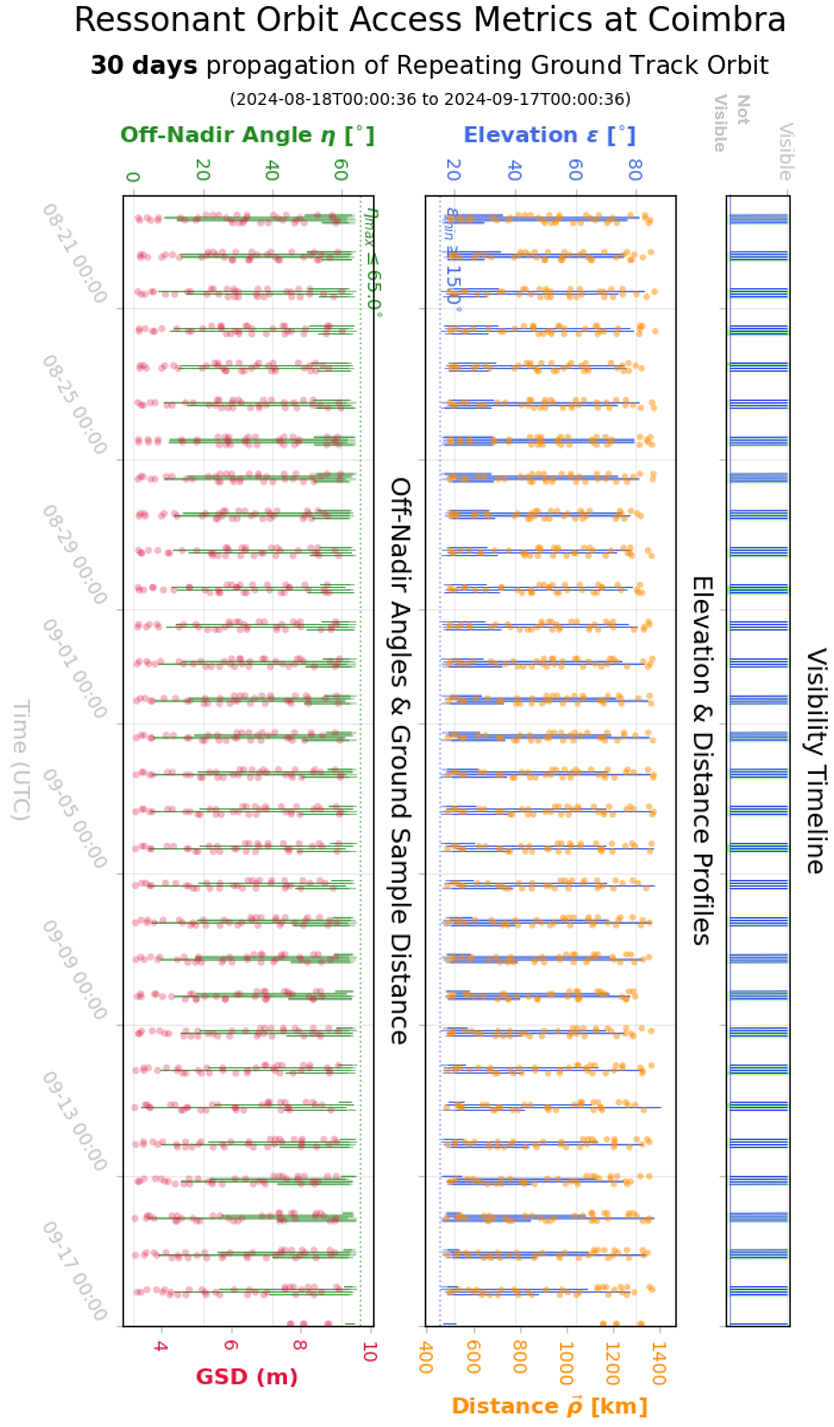
\includegraphics[width=0.8\linewidth]{images/RGTO_maps_Coimbra_Thirty_days.png}
    \caption{\footnotesize{Observation metrics of 30-day uncontrolled RGTO seed propagation over Coimbra ($\tau=15/1$, $h \approx 488$\,km). The four-pass daily pattern persists but elevation and off-nadir metrics begin to degrade toward day~30, indicating the onset of resonance drift.}}
    \label{fig:RGTO_maps_Coimbra_Thirty_days}
\end{figure}

\subsection{1-Year Uncontrolled Propagation}

To quantify the long-term resonance departure, the propagation is extended to one year without any orbit-maintenance manoeuvres.  Figure~\ref{fig:stationkeeping_Off} presents the orbital-element evolution over this period.  The semi-major axis decreases monotonically under atmospheric drag, and the repeating ground-track condition is progressively lost: the sub-satellite trace drifts across all longitudes, and the satellite ground track ceases to be confined to the Coimbra latitude band.  At the end of one year the orbit no longer bears any resemblance to the original resonance pattern. The satellite effectively covers the globe rather than revisiting the target domain.

This result confirms that uncontrolled drag is incompatible with sustained RGTO resonance and motivates the station-keeping strategy introduced in the next section.

\begin{figure}[H]
    \centering
    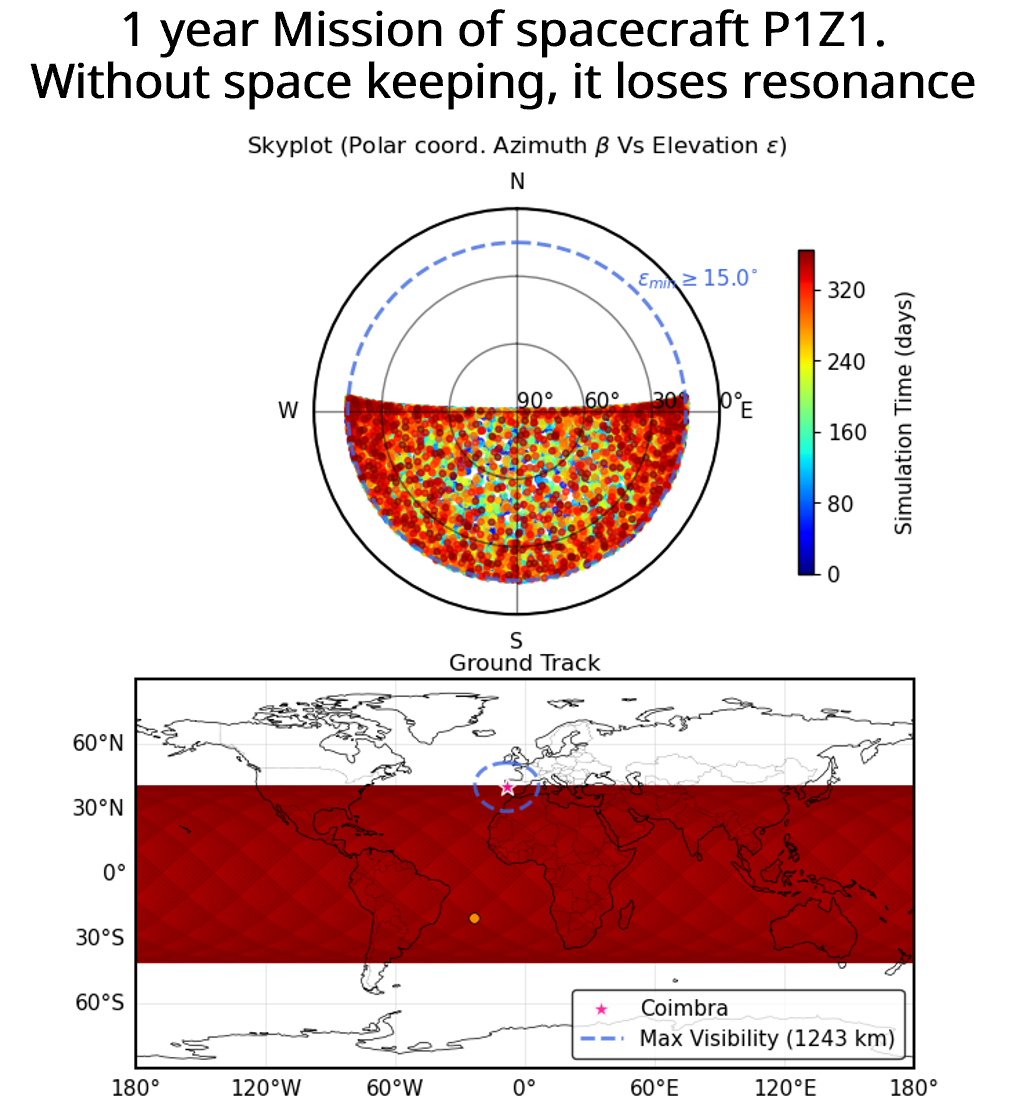
\includegraphics[width=0.8\linewidth]{images/stationkeeping_Off.png}
    \caption{\footnotesize{Orbital-element evolution over 1~year without station-keeping for the RGTO seed orbit.  Atmospheric drag causes a semi-major axis decay, leading to complete loss of the repeating ground-track resonance.}}
    \label{fig:stationkeeping_Off}
\end{figure}

\section{Station-Keeping Method and Results}\label{sec:sk_method}

A simplified altitude-maintenance algorithm is implemented in NASA GMAT to evaluate whether the RGTO resonance can be preserved over the mission lifetime.  The algorithm, illustrated in Fig.~\ref{fig:station_keeping_GMAT_algorithm}, operates as follows.  During the one-year propagation, the spacecraft altitude is continuously monitored.  When the altitude drops below the threshold $h_{\mathrm{thr}} = 480$\,km due to atmospheric drag, the algorithm is triggered:
\begin{enumerate}
    \item The satellite is propagated forward until it crosses the target latitude $\phi_{\mathrm{lat}} = 40.2^{\circ}$\,N (the Coimbra resonance latitude).
    \item At this position, an impulsive prograde burn ($\Delta V_1$) is applied to raise the orbit to approximately $h \approx 488$\,km.
    \item The orbital propagation continues until the subsequent apoapsis, where a second impulsive burn ($\Delta V_2$) circularises the orbit, restoring near-zero eccentricity.
\end{enumerate}
This two-burn sequence restores an orbit close to the original seed conditions.  The algorithm then resumes passive propagation until the next threshold crossing.  Note that an ideal impulsive-burn model is assumed: no propellant mass decrement is applied, and the spacecraft mass remains constant throughout.  A more detailed propulsion trade-off---including fuel budget, thruster sizing, and the impact of finite-burn duration---is deferred to future work.

\begin{figure}[H]
    \centering
    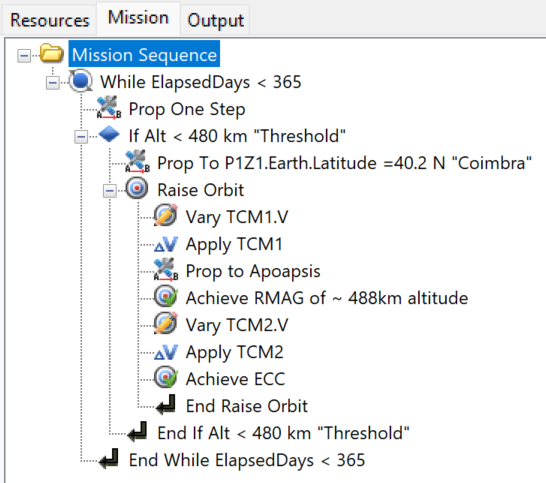
\includegraphics[width=0.4\linewidth]{images/station_keeping_GMAT_algorithm.png}
    \caption{\footnotesize{Simplified station-keeping algorithm implemented in GMAT.  When $h < 480$\,km, the spacecraft propagates to latitude $\phi = 40.2^{\circ}$, applies a prograde burn to raise the apoapsis to $\sim$488\,km, then circularises at apoapsis.}}
    \label{fig:station_keeping_GMAT_algorithm}
\end{figure}

Using this method, the same spacecraft and force-model configuration is propagated for one year under the same initial conditions as the uncontrolled case (Fig.~\ref{fig:stationkeeping_Off}).  The resulting orbital-element evolution is shown in Fig.~\ref{fig:stationkeeping_On}.  The resonance pattern is substantially better preserved compared with the uncontrolled case: the ground track remains concentrated around the Coimbra latitude band, and the four-pass daily observation sequence is largely maintained.  Residual drift is still visible, suggesting that the algorithm could be refined, but the result demonstrates that it is feasible to sustain the RGTO resonance with a simple low-thrust strategy.

\begin{figure}[H]
    \centering
    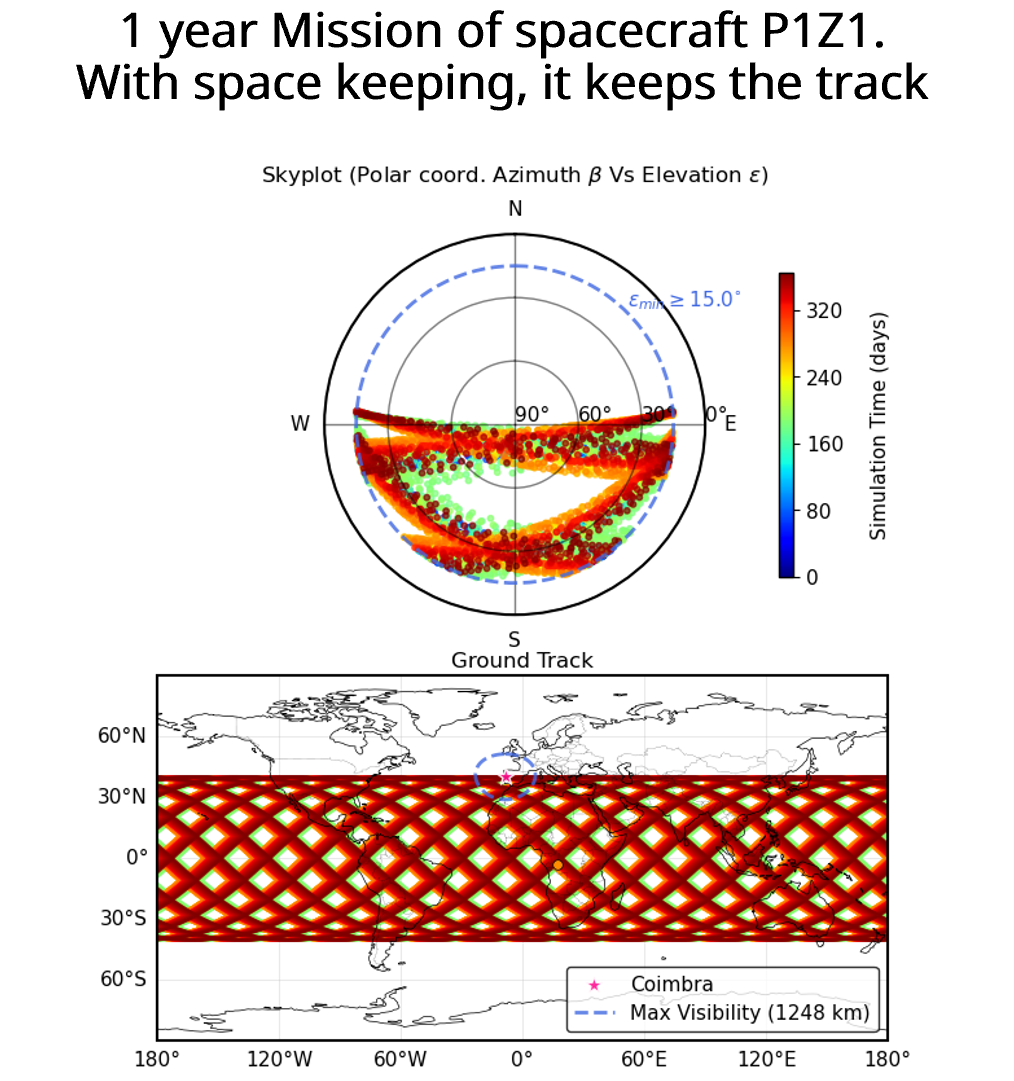
\includegraphics[width=0.8\linewidth]{images/stationkeeping_On.png}
    \caption{\footnotesize{Orbital-element evolution over 1~year with the station-keeping algorithm enabled.  The repeating ground-track resonance is substantially preserved; residual drift suggests the algorithm could be further refined.}}
    \label{fig:stationkeeping_On}
\end{figure}

\section{Altitude Evolution and End-of-Life Results}\label{sec:sk_altitude_eol}

Figure~\ref{fig:stationkeepingOn_hVSt} shows the altitude history for the one-year station-kept propagation.  Four burn events occur during the year, each triggered when $h$ drops below 480\,km.  After each two-burn correction the altitude is restored to $\sim$488\,km, and between burns the altitude remains above $\sim$482.5\,km.  This confirms that the simplified algorithm is sufficient to maintain the resonance altitude band over a one-year period with only four manoeuvre pairs per year.

\begin{figure}[H]
    \centering
    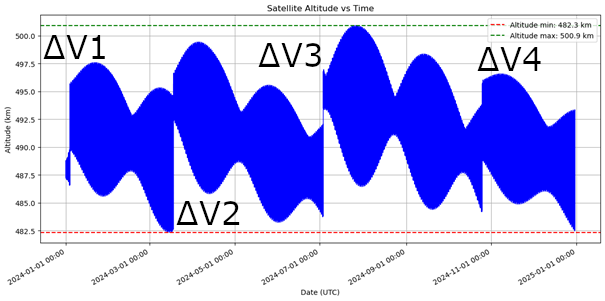
\includegraphics[width=0.75\linewidth]{images/stationkeepingOn_hVSt.png}
    \caption{\footnotesize{Altitude vs.\ time over 1~year with station-keeping.  Four burn events (triggered at $h < 480$\,km) restore the orbit to $\sim$488\,km; between burns the altitude remains above $\sim$482.5\,km.}}
    \label{fig:stationkeepingOn_hVSt}
\end{figure}

\subsubsection{Lifetime of Resonant Orbit}
Figure~\ref{fig:deorbiting_RGTO_Coimbra} presents the uncontrolled altitude decay from the initial $h_0 \approx 488$\,km.  Without station-keeping, the drag-induced descent accelerates as the spacecraft enters denser atmospheric layers, and the orbit reaches the end-of-life altitude ($h_{\mathrm{EOL}} \approx 285$\,km) after approximately 2.68~years.  This constitutes the natural orbital lifetime of the RGTO seed orbit for the assumed spacecraft parameters.


\begin{figure}[H]
    \centering
    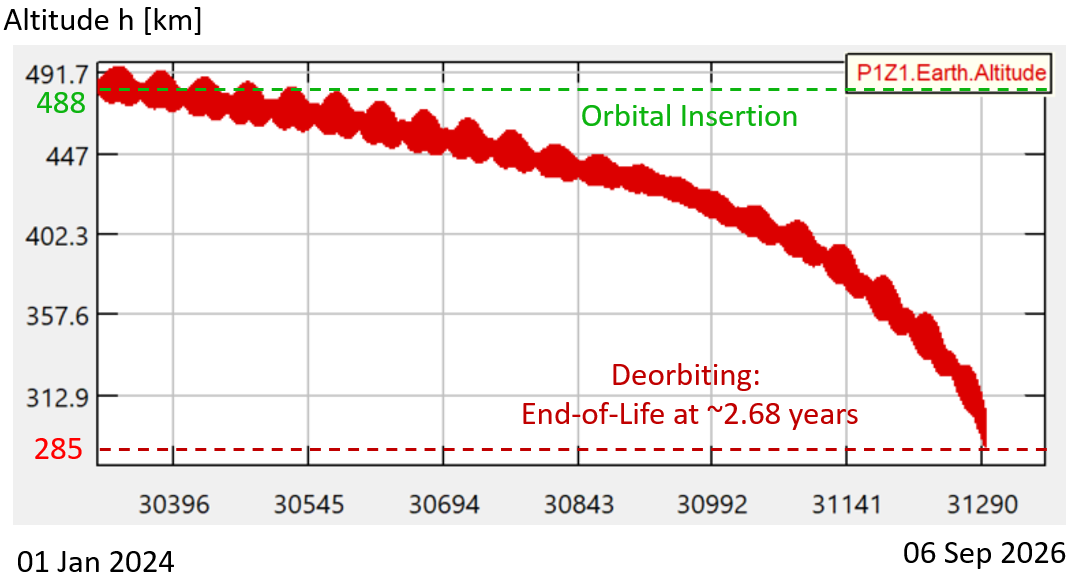
\includegraphics[width=0.6\linewidth]{images/deorbiting_RGTO_Coimbra.png}
    \caption{\footnotesize{Orbital altitude decay of object P1Z1 plotted against the UTC Modified Julian Date. The data illustrates the trajectory from an initial orbital insertion at $h = 488$ km on 01 Jan 202 (UTC) down to a final deorbiting altitude of 285 km on 06 Sep 2026 (UTC), spanning a total timeframe of 979.5 days (approximately 2.68 years).}}
    \label{fig:deorbiting_RGTO_Coimbra}
\end{figure}




\section{Summary}

The analysis demonstrates that the RGTO seed orbit $\vec{\mathbf{A}}^{\,\mathrm{RGTO}^{\,2}}{}_{0,\,\mathrm{Coimbra}}$ maintains the repeating ground-track resonance for approximately 7--30~days under uncontrolled propagation before drag-induced drift degrades the observation pattern.  A simplified two-burn station-keeping algorithm, triggered when the altitude drops below 480\,km, successfully restores the resonance with only four correction events per year.  Without station-keeping, the uncontrolled orbital lifetime is approximately 2.68~years.  These results confirm that the RGTO resonance is operationally sustainable with modest propulsive, but station keeping function is mandatory in a spacecraft system to provide a cost effective mission.  This analysis effort provide the lifetime warranty for the constellation design developed in the main text.

\chapter{Walker RGTO Constellation Parameters}\label{app:constellation_tables}

This appendix collects the full orbital-element tables for the three Walker RGTO constellation candidates evaluated in Chapter~\ref{73-constellation-design-architectures}.  All satellites share the RGTO seed orbit described in Table~\ref{tab:rgto_parameters_coimbra} ($\tau=15/1$, $e=0.001$, $i=40.20329^{\circ}$, $\omega=0^{\circ}$), with $\Omega_{\mathrm{ref}}=100^{\circ}$ chosen to align $P_1S_1$ with the 18~August 15:00\,LT fire-peak pass over Coimbra.

\begin{table}[H]
\centering
\caption{\footnotesize{Walker RGTO constellation satellite parameters.  \textbf{Left}: Baseline $\mathcal{C}_{15/5/72}$ ($t_{\mathrm{rev}} \approx 33$\,min, uniform full-day coverage).  \textbf{Centre}: Candidate $\mathcal{C}_{12/4/90}$ ($t_{\mathrm{rev}} \approx 33$\,min, coverage gaps).  \textbf{Right}: High-cadence variant $\mathcal{C}_{20/5/72}$ ($t_{\mathrm{rev}} \approx 25$\,min).}}
\label{tab:walker_constellations}
\smallskip
\footnotesize
\setlength{\tabcolsep}{5pt}
\begin{minipage}[t]{0.32\linewidth}
\centering
\textbf{$\mathcal{C}_{15/5/72}$}\\[2pt]
\begin{tabular}{c c r r}
\toprule
Pl & $S_k$ & $\Omega$ & $\nu_0$ \\
\midrule
\multirow{3}{*}{$P_1$} & $S_1$  & 100 &   0 \\
                        & $S_2$  & 100 & 120 \\
                        & $S_3$  & 100 & 240 \\
\midrule
\multirow{3}{*}{$P_2$} & $S_4$  & 172 &   0 \\
                        & $S_5$  & 172 & 120 \\
                        & $S_6$  & 172 & 240 \\
\midrule
\multirow{3}{*}{$P_3$} & $S_7$  & 244 &   0 \\
                        & $S_8$  & 244 & 120 \\
                        & $S_9$  & 244 & 240 \\
\midrule
\multirow{3}{*}{$P_4$} & $S_{10}$ & 316 &   0 \\
                        & $S_{11}$ & 316 & 120 \\
                        & $S_{12}$ & 316 & 240 \\
\midrule
\multirow{3}{*}{$P_5$} & $S_{13}$ &  28 &   0 \\
                        & $S_{14}$ &  28 & 120 \\
                        & $S_{15}$ &  28 & 240 \\
\bottomrule
\end{tabular}
\end{minipage}%
\hfill
\begin{minipage}[t]{0.32\linewidth}
\centering
\textbf{$\mathcal{C}_{12/4/90}$}\\[2pt]
\begin{tabular}{c c r r}
\toprule
Pl & $S_k$ & $\Omega$ & $\nu_0$ \\
\midrule
\multirow{3}{*}{$P_1$} & $S_1$  & 100 &   0 \\
                        & $S_2$  & 100 & 120 \\
                        & $S_3$  & 100 & 240 \\
\midrule
\multirow{3}{*}{$P_2$} & $S_4$  & 190 &   0 \\
                        & $S_5$  & 190 & 120 \\
                        & $S_6$  & 190 & 240 \\
\midrule
\multirow{3}{*}{$P_3$} & $S_7$  & 280 &   0 \\
                        & $S_8$  & 280 & 120 \\
                        & $S_9$  & 280 & 240 \\
\midrule
\multirow{3}{*}{$P_4$} & $S_{10}$ &  10 &   0 \\
                        & $S_{11}$ &  10 & 120 \\
                        & $S_{12}$ &  10 & 240 \\
\bottomrule
\end{tabular}
\end{minipage}%
\hfill
\begin{minipage}[t]{0.32\linewidth}
\centering
\textbf{$\mathcal{C}_{20/5/72}$}\\[2pt]
\begin{tabular}{c c r r}
\toprule
Pl & $S_k$ & $\Omega$ & $\nu_0$ \\
\midrule
\multirow{4}{*}{$P_1$} & $S_1$  & 100 &   0 \\
                        & $S_2$  & 100 &  90 \\
                        & $S_3$  & 100 & 180 \\
                        & $S_4$  & 100 & 270 \\
\midrule
\multirow{4}{*}{$P_2$} & $S_5$  & 172 &   0 \\
                        & $S_6$  & 172 &  90 \\
                        & $S_7$  & 172 & 180 \\
                        & $S_8$  & 172 & 270 \\
\midrule
\multirow{4}{*}{$P_3$} & $S_9$  & 244 &   0 \\
                        & $S_{10}$ & 244 &  90 \\
                        & $S_{11}$ & 244 & 180 \\
                        & $S_{12}$ & 244 & 270 \\
\midrule
\multirow{4}{*}{$P_4$} & $S_{13}$ & 316 &   0 \\
                        & $S_{14}$ & 316 &  90 \\
                        & $S_{15}$ & 316 & 180 \\
                        & $S_{16}$ & 316 & 270 \\
\midrule
\multirow{4}{*}{$P_5$} & $S_{17}$ &  28 &   0 \\
                        & $S_{18}$ &  28 &  90 \\
                        & $S_{19}$ &  28 & 180 \\
                        & $S_{20}$ &  28 & 270 \\
\bottomrule
\end{tabular}
\end{minipage}
\end{table}

\chapter{Requirements Appendix}\label{app:requirements}

This appendix provides an example of how to use the requirements tracking system. 
You can define requirements using the `\. requirement` command or creating an inline requirement with `\ inlineReq{R-ID}` and reference them in your text using `\ reqRef{R-ID}`.
Once requirements are defined, you can reference them from anywhere in your document. This is useful for tracing how the system's design and implementation satisfy the initial requirements.

example:

\begin{enumerate}\setlength{\itemsep}{0pt}\setlength{\parskip}{0pt}\setlength{\parsep}{0pt}
\item \textbf{Diagnosis of fire-resilience states \inlineReq{R1}}\footnote{[\rightarrow R\#] refers to the requirement number \# being created at this point. Full description of the requirment is found in the end of each chapter, i.e \S \ref{sec:requirements_level1}.The requirements framework adopted in this work is detailed in Appendix~\ref{app:se_approach} and \S\ref{sec:requirements_level1}.}
\item \textbf{Anticipation of ignitions \inlineReq{R2}}
\item \textbf{Near--real-time identification of hotspots \inlineReq{R3}}
\item \textbf{Near--real-time monitoring of fire-front evolution \inlineReq{R4}}
\item \textbf{All weather, cloud/smoke-penetrating, day/night capability \inlineReq{R5}}
\end{enumerate}


% The descripiton of the `.\\requirement` command has the following structure:
% \requirement{<ID>}{<Title>}{<Description>}{<Type>}{<Tags>}
% - <ID>: A unique identifier for the requirement (e.g., R-01).
% - <Title>: A short, descriptive title.
% - <Description>: A detailed explanation of the requirement.
% - <Type>: The category of the requirement (e.g., Functional, Non-Functional, Performance, Security).
% - <Tags>: Comma-separated tags for filtering or grouping (e.g., UI, Database, API).

\section{Example: Mission Objectives (Chapter 1)}\label{sec:app_req_ch1}
\subsection{Mission Earth Observation Products}

The following requirements define the primary Earth Observation inputs and products necessary to support wildfire resilience and monitoring objectives.

\requirement{R1}{Fire Resilience Inputs}{Provide EO measurement products sufficient for external wildfire-resilience indices; e.g., vegetation state \& dynamics, moisture, thermal regime, and structure; cadence and spectral bands: TBD.}{Mission}{EO product}

\requirement{R2}{Anticipation of ignitions}{Provide sufficient EO capabilities for third-party short-term ignition-risk assessment and forecasts.}{Mission}{EO product}

\requirement{R3}{Near-real-time identification of hotspots}{Provide capability for third-party near-real-time hotspot detection alerts with geo-referenced location and confidence; minimum detectable size, geolocation accuracy, and alert latency: TBD.}{Mission}{EO product}

\requirement{R4}{Near-real-time monitoring of fire-front evolution}{Provide capability for near-real-time third-party products describing the fire front perimeter and spread rate during overpass; update cadence, geolocation accuracy, and revisit: TBD.}{Mission}{EO product}






\chapter{Systems Engineering Methodological Approach}\label{app:se_approach}

\begin{figure}[H]
	\centering
	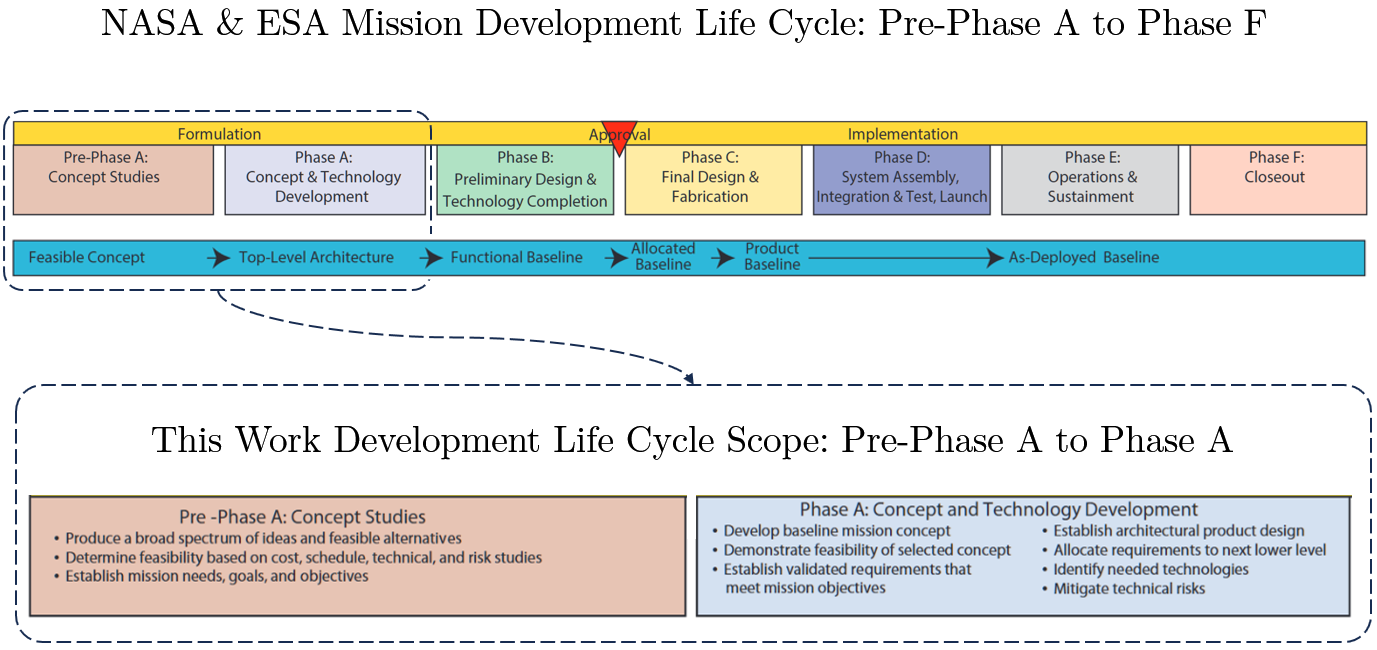
\includegraphics[width=1\textwidth]{images/c1.4_NASA_development_lifecycle.png}
	\caption[{NASA \& ESA Systems Engineering Development Life-Cycle. This work only covers Pre-Phase A and Phase A. Adapted from}]{NASA \& ESA Systems Engineering Development Life-Cycle. This work only covers Pre-Phase A and Phase A. Adapted from \parencite{SEHandbook}.}
	\label{fig:nasa-lifecycle}
\end{figure}

NASA's space-flight project life cycle is organized for complex product development involving multidisciplinary teams and disciplines \cite{SEHandbook}. As the mission development involves intricate requirements development, using a systems engineering approach enables this project to deliver a mission baseline solution in a scientific and systems engineering language, allowing further future work to be easily transferred and developed within engineering and other disciplines' frameworks. 

The scope of the SE life-cycle is summarized in Figure \ref{fig:nasa-lifecycle}. The life-cycle partitions work into discrete phases, separated by Key Decision Points (KDPs) where readiness to advance is assessed. Pre-Phase A (Concept Studies) surveys mission needs, feasibility, and trades and constraints. Phase A (Concept \& Technology Development) matures the mission concept, baselines initial system-level requirements, identifies technology gaps, establishes architectural product design, demonstrates the feasibility of the selected concept, and allocates requirements to the next lower system level. Phase B (Preliminary Design \& Technology Completion) completes technology maturation and the preliminary design. Phase C (Final Design \& Fabrication) finalizes detailed design and builds the flight system. Phase D (System Assembly, Integration \& Test, Launch \& Checkout) integrates and verifies the system and conducts launch/commissioning. Phase E (Operations \& Sustainment) conducts on-orbit operations, and Phase F (Closeout) decommissions and archives. 

The scope, methods, and results of this work are contained only in Pre-Phase A and Phase A, as these phases establish feasibility, architecture, and early requirements that drive all downstream design decisions.


\end{appendices}


%--- BIBLIOGRAPHY ---
\printbibliography[heading=bibintoc, title={References}]


% Reset chapter title format for appendices (display on separate page)
\titleformat{\chapter}[display]
{\normalfont\huge\bfseries}{\chaptertitlename\ \thechapter}{20pt}{\Huge}




%\chapter{Institutions and Operational Flows of Rural Fire Management in Portugal (AGIF/SGIFR)}
\label{appendix-agif_pt_fire_combat_system_en}

Portugal’s rural-fire governance is organized under the \emph{Integrated Rural Fire Management System} (SGIFR), established by \emph{Decree–Law No.\,82/2021} and supported by a public, inter-institutional portal. The \emph{Agency for Integrated Rural Fire Management} (AGIF) provides strategic planning, inter-ministerial coordination, and system evaluation, issuing guidance and coordination models that link the operational entities across the entire fire cycle \cite{DL82-2021,SGIFR-Portal,AGIF-SGIFR,SGIFR-Leg}.

Functionally, responsibilities are shared by five principal actors. \textbf{AGIF} leads national strategy, clarifies roles, monitors implementation of the national plan, and promotes continuous improvement through lessons-learned processes \cite{AGIF-SGIFR,SGIFR-Portal}. The \textbf{ICNF} (Institute for Nature Conservation and Forests) manages public forest assets and provides daily fire-danger indices and rules for the use of fire, supporting local preparedness and prevention \cite{ICNF-Risco,ICNF-PIR,IPMA-PIR}. The \textbf{ANEPC} (National Authority for Emergency and Civil Protection) commands the emergency response and activates the \emph{Special Rural Firefighting Dispositive} (\emph{DECIR}) via the national operational directive, tasking ground, aerial, and command-and-control assets \cite{ANEPC-DECIR-2025,ANEPC-site}. The \textbf{GNR} (National Republican Guard) strengthens prevention through surveillance and enforcement—patrols, detection, and reporting of infractions—thus contributing to both prevention and the effectiveness of response \cite{GNR-noticias}. Finally, the \textbf{PJ} (Judiciary Police) investigates wildfire causes and produces forensic knowledge that feeds back into prevention policies and operational practice \cite{PJ-incendio}.

Operationally, the system follows a continuous cycle. First, \emph{planning and coordination} (AGIF) define the vision and governance framework. Next, \emph{prevention and preparedness} (ICNF, municipalities, and GNR) deliver fuel-management, land-use measures, and public outreach, guided by fire-danger indices and rules for controlled burning. When ignitions occur, \emph{response} (ANEPC/DECIR) coordinates operations and resources. Finally, \emph{investigation} (PJ) determines causes and returns evidence to the system, closing the loop with continuous improvement \cite{DL82-2021,AGIF-SGIFR,ICNF-Risco,ANEPC-DECIR-2025,PJ-incendio}.

\begin{figure}[H]
    \centering
    
\includegraphics[width=0.9\textwidth]{appendix/data/AGIF_high_level.png}
    \caption{\footnotesize{Update with official: High level Institutions and operational flows of Agency for Integrated Rural Fire Management}}
    \label{fig:appendix-agif_pt_fire_combat_system_high_level}
\end{figure}

\begin{figure}[H]
    \centering
    
\includegraphics[width=0.9\textwidth]{appendix/data/AGIF_detailed.png}
    \caption{\footnotesize{Update with official: Detailed Institutions and operational flows of Agency for Integrated Rural Fire Management}}
    \label{fig:appendix-agif_pt_fire_combat_system_detailed}
\end{figure}


% To include an external PDF:
% \includepdf[pages={-}]{path/to/appendix.pdf}
%\end{appendix}



\end{document}
